\PassOptionsToPackage{svgnames}{xcolor} %para los myblock - ha de estar al principio 
\documentclass[a5paper, 10pt, spanish]{book}
\usepackage[utf8]{inputenc}
\usepackage[T1]{fontenc}
\usepackage[spanish]{babel}
\usepackage{float} %posicionar figuras
\usepackage{multicol}
\usepackage{multirow} % esto hará falta para figuras casi seguro
\usepackage{amsmath} %ecuaciones bien
\usepackage{amsthm}
\usepackage{amsfonts}
\usepackage{amssymb}
\usepackage{graphicx} %opciones /includegraphics[...]
\usepackage{indentfirst} % sangria de primera linea
%\setlength{\parindent}{0cm} %elimino sangrado 1a linea
\usepackage{fancyhdr}
\usepackage{caption}
\usepackage{subcaption}
\usepackage{esint} % integrales mejor

\usepackage[top=1.8cm, bottom=1.6cm, left=2cm, right=1.6cm]{geometry} % márgenes (para encuadernado-book: impares más a la izquda, pares más a la dcha.
\usepackage{comment} % comment environment
\usepackage{physics}
\usepackage{enumerate}
%\usepackage{footnote} 
%\makesavenoteenv{tabular} 
%\makesavenoteenv{table}%% write footnotes on tables
%\setlength{\parskip}{10px} %espacio parrafos error con teoremas
%\usepackage{verbatim} % comentarios
\usepackage{comment} % comentarios
\usepackage{accents}
\usepackage{pdfpages} %insertar pdfs

\usepackage{ragged2e} % para  \justifying después de fcolorbox-parbox


\widowpenalty10000
\clubpenalty10000
\setcounter{tocdepth}{3}

%FLOAT EQNS LEFT
\usepackage{nccmath} 
\makeatletter
\newcommand{\leqnomode}{\tagsleft@true}
\newcommand{\reqnomode}{\tagsleft@false}
\makeatother

\usepackage{mathtools} %alinear matrices izqda
%\begin{equation}
%\begin{pmatrix*}[l]
%63 & 71 & 2\\
%6 & 829 & 12\\
%599 & 9 & 361
%\end{pmatrix*}
%\end{equation}

 
%% estos comandos van a arreglarme bastante la vida
%\newcommand{\pd}[2]{\frac{\partial#1}{\partial#2}}
%\newcommand{\td}[2]{\frac{\mathrm{d}#1}{\mathrm{d}#2}}
%\newcommand{\dif}[0]{\mathrm{d}}

%\languagepath{spanish}
%\uselanguage{spanish}
%\deftranslation[to=spanish]{Theorem}{Teorema.}
%\deftranslation[to=spanish]{theorem}{teorema.}

\definecolor{roig}{RGB}{196,49,24}
\definecolor{morat}{RGB}{131,54,147}
\definecolor{verd}{RGB}{85,107,47}
\definecolor{gris}{RGB}{100,100,100}
\definecolor{blau}{RGB}{0,0,100}
\definecolor{fondoblau}{RGB}{232,255,255}
\definecolor{fondoroig}{RGB}{245,194,194}
\definecolor{fondoverd}{RGB}{209,240,192}

\newcommand{\subrayado}[1]{\colorbox{yellow}{$\displaystyle #1$}} %fosforito ecuaciones begin{eq... 

\newtheorem{lema}{Lema}
\newtheorem{teor}{Teorema}
\newtheorem{coro}{Corolario}
\newtheorem{prop}{Proposición}
\newtheorem{defi}{Definición}
\newtheorem{axio}{Axioma}
\newtheorem{ejem}{Ejemplo}
\newtheorem{ejre}{Ejercicio resuelto}
\newtheorem{ejer}{Ejercicio.}
\newtheorem{ayud}{Ayuda.}
\newtheorem{solu}{Solución.}

\numberwithin{equation}{chapter}
\numberwithin{lema}{chapter}
\numberwithin{teor}{chapter}
\numberwithin{coro}{chapter}
\numberwithin{prop}{chapter}
\numberwithin{defi}{chapter}
\numberwithin{axio}{chapter}
\numberwithin{ejem}{chapter}
\numberwithin{ejre}{chapter}
\numberwithin{ejer}{chapter}
\numberwithin{ayud}{chapter}
\numberwithin{solu}{chapter}

%\usepackage{longtable} % para tablas largas

\usepackage{fancyhdr}
\pagestyle{fancy}
\renewcommand{\chaptermark}[1]{%
\markboth{\thechapter.\ #1}{}}
%\newcommand{\TheAuthor}{Ignacio Vallés Oriola} % As given in documentation of **fancyhdr**
%\newcommand{\Author}[1]{\renewcommand{\TheAuthor}{#1}}
\fancyhead{} % clear all fields

%\lhead{\leftmark}
%\rhead{Ignacio Vallés Oriola}
\fancyhead[LO]{\MakeUppercase{\leftmark}}
\fancyhead[RE]{\nouppercase{\rightmark}}
\fancyhead[LE, RO]{Ignacio Vallés Oriola}

%demostraciones sin frase ni punto inicial
\makeatletter
\newenvironment{proofw}{\par
  \pushQED{\qed}%
  \normalfont \topsep6\p@\@plus6\p@\relax
  \trivlist
  \item[]\ignorespaces
}{%
  \popQED\endtrivlist\@endpefalse
}
\makeatother 

\usepackage{soul} %tachado, usando \textst{lo que se desea tachar} No vale en ecuaciones.
\usepackage[makeroom]{cancel} % tachar en equaciones \cancel{a tachar}; \bcancel tacha al revés ; \xcancel tacha con x; \cancelto {0 (o \infty}{expresion a tachar} flecha con 0 o infty


%%% bloques
% blocks
% \PassOptionsToPackage{svgnames}{xcolor}   ---- en primera línea
\usepackage{tcolorbox}
\tcbuselibrary{skins,breakable}
\usetikzlibrary{shadings,shadows}
    
\newenvironment{myexampleblock}[1]{%
    \tcolorbox[beamer,%
    noparskip,breakable,
    colback=Honeydew,colframe=DarkGreen,%
    colbacklower=LimeGreen!75!Honeydew,%
    title={#1}]}%
    {\endtcolorbox}

  
\newenvironment{myalertblock}[1]{%
    \tcolorbox[beamer,%
    noparskip,breakable,
    colback=LavenderBlush,colframe=DarkRed,%
    colbacklower=Tomato!75!LavenderBlush,%
    title={#1}]}%
    {\endtcolorbox}

\newenvironment{myblock}[1]{%
    \tcolorbox[beamer,%
    noparskip,breakable,
    colback=AliceBlue,colframe=DarkBlue,%
    colbacklower=DarkBlue!75!AliceBlue,%
    title={#1}]}%
    {\endtcolorbox}
    


\renewcommand{\baselinestretch}{1.2} %interlineado
\setlength{\parskip}{2mm} %espacio entre párrafos

\title{Cálculo infinitesimal en una variable \\ (avanzado) para bachillerato.} 
%	\\
% -  \\ 
%\large{(ampliado)}}

\author{Ignacio Vallés Oriola.}
\date{}

\setcounter{tocdepth}{2} %hasta segundo nivel secc

%\rotatebox{180}{\leftline{\textcolor{gris}{texto a escribir }}}

% $\divideontimes$ ejercicio difícil

%\rotatebox{180}{\leftline{\textcolor{gris}{\scriptsize{Sol: $\frac 1 {x^2}$ no está definida en $x0=\in [-3,2]$}}}}. 
%!!!!!!!Texto escrito de dcha a izqda en cualquier parte del texto.

\setlength{\parindent}{5 mm} %elimina sangrado primera línea

%*************. \boldsymbol{$fórmula en negrita$}


% ***********.  numero tachado horizontalmente --  $\text{\textst{5}}$
\spanishdecimal{.}


%\usepackage{enumitem} %para usar \begin{itemize}[noitemsep] eliminando espaciados en lista

%\includeonly{TEMA12_chapter} %para ver solo esto, o separado por comas, varios

\begin{document}

\begin{titlepage}
	\centering
	\vspace*{\fill}
	{\scshape\LARGE ÁLGEBRA LINEAL Y GEOMETRIA (avanzadas) PARA BACHILLERATO\par}
	\vspace{1cm}
	{\Large Ignacio Vallés Oriola \par}
	\vspace{3cm}
	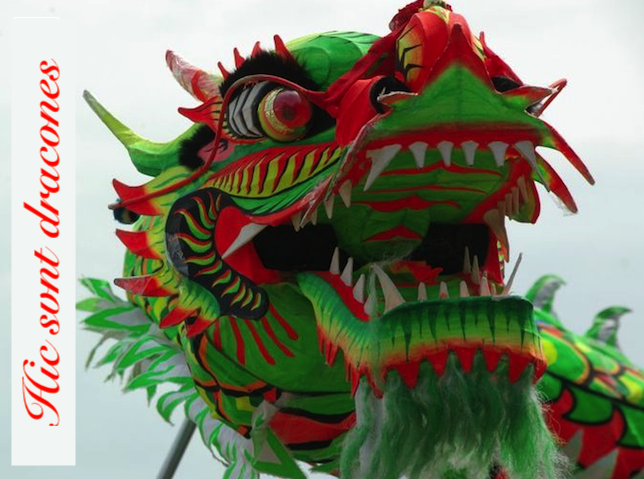
\includegraphics[width=0.75\textwidth]{imagenes/hic-svnt-dracones}
	\vspace{3cm}
\end{titlepage}

\tableofcontents

\section{Intoducción.}

La confección de este texto es fruto de una larga experiencia como profesor de matemáticas de secundaria y para ello me he basado en mis más de treinta años de docencia  y en la de tantos autores que han contribuido a la explicación de estos conceptos a multitud de alumnos. He usado también apuntes y problemas de libros de texto de segundo de bachillerato: Anaya, Marea Verde, SM, Santillana, Editex, Edunsa, Alhambra, Marfil, Ecir, Bruno, etc. Así como apuntes y ejercicios encontrados en la web y pruebas de acceso a la universidad de distintas comunidades autónomas. Gracias a todos ellos por su inestimable ayuda para la confección de este pequeño texto que espero que sirva a alguien y que escribo libre de todo tipo de derechos. En particular, me han sido de mucha utilidad los `Apuntes de Álgebra' de José Salvador Cánovas Peña, profesor del departamento de Matemática Aplicada y Estadística de la Universidad Politécnica de Cartagena.

Los apartados, teoremas y los ejercicios de mayor nivel estarán marcados con el símbolo $\divideontimes$. Exceden los contenidos de un curso de segundo de bachillerato pero son altamente recomendables para el alumnado que necesite ampliar sus conocimientos matemáticos en cursos posteriores.


\subsubsection{Cómo estudiar matemáticas}

 
Las Matemáticas son una asignatura que no deja indiferente a ningún estudiante. Algunos la aman y otros la odian; siendo este segundo grupo mucho más numeroso que el primero en la mayoría de las ocasiones. Sin embargo, muchos de los estudiantes que odian las matemáticas lo hacen porque no saben cómo estudiarlas para obtener buenos resultados.

Las Matemáticas son una de esas asignaturas en las que las horas de estudio no tienen una relación directa con la nota. Por mucho que hayas estudiado, si no eres capaz de solucionar el problema del examen, estás perdido. No obstante, existen algunas técnicas para aprender matemáticas que pueden hacer que, independientemente de tu nivel, le saques más partido a tu tiempo de estudio y aumentes tus probabilidades de éxito. ¡Hasta es posible que te acabes uniendo al grupo de amantes de las matemáticas!

\emph{Cómo Estudiar Matemáticas:}
 
\begin{enumerate}
	 

\item Práctica, Práctica y Más Práctica

Es imposible aprender matemáticas leyendo y escuchando. Para aprender matemáticas hay que ponerse el mono de trabajo y lanzarse a hacer ejercicios matemáticos. Cuanto más practiques, mejor. Cada ejercicio tiene sus particularidades y es importante haber realizado el máximo número de ejercicios posibles antes de enfrentarnos al examen. Este punto es el más importante de todos y la base del resto de técnicas para estudiar matemáticas de esta lista.

Una vez que entendiste los ejemplos explicados en clase, desarrolla ejercicios o problemas con solución para complementar tus conocimientos. Trata de hacerlos sin ver la respuesta y luego, si ni lo puedes terminar, ayúdate de la solución y sigue desarrollando, siempre preguntándote ?`por qué se realiza dicho paso? Se trata de que poco a poco no tengas necesidad de utilizar las soluciones y llegará el momento, después de unos pocos ejercicios, en que ya no necesites de ellas para desarrollar y entender completamente los problemas

No pienses que escuchando la explicación de muchos ejercicios y problemas, donde un profesor te explica y entiendes un 100$\%$, es lo más importante para aprender Matemáticas. La clave del éxito es \emph{¡PRACTICAR!}

\item Revisa los Errores

Cuando estés practicando con ejercicios, es muy importante que compruebes los resultados y, más importante aún, que te detengas en la parte que has fallado y examines el proceso en detalle hasta asimilarlo. De nada sirve comparar resultados si no sabes en qué te has equivocado. Por eso es conveniente que tengas unos buenos apuntes con problemas resueltos. De esta manera, evitarás cometer los mismos fallos en el futuro. También es recomendable apuntar todos tus fallos y repasarlos repetidamente antes del examen.

Toma buenos apuntes: Sé ordenado, utiliza un solo cuaderno para el curso y escribe claramente usando, en lo posible, tus propias palabras para que puedas entender cuando estudies. Copia todo lo que el profesor diga y escriba en la pizarra, anotando los porqués de cada paso, ya que uno siempre puede olvidar lo escuchado y cuando vuelvas a leer tus apuntes podrás recordarlos rápidamente.

Observa y apunta si el profesor hace hincapié en ciertos puntos basándose en repeticiones, ejemplos, diagramas, comentarios extensos, etc., éstos son casi siempre parte importante de los temas.

\item Domina los Conceptos Clave

¡No intentes aprenderte los problemas de memoria! Los problemas matemáticos pueden tener miles de variantes y particularidades, por lo que es inútil aprendernos problemas de memoria sin entenderlos. Es cambio, es mucho más efectivo dominar los conceptos importantes y el proceso de resolución de los problemas.

Recuerda que las Matemáticas son una asignatura secuencial, por lo que es importante asentar una base firme dominando los conceptos clave y teniendo claras las fórmulas matemáticas esenciales.

\item Consulta tus Dudas

Puede que en muchas ocasiones te sientas atascado en una parte de un problema o que simplemente no entiendas el proceso. Lo común en estos casos es simplemente pasar de ese problema y pasar al siguiente. Sin embargo, es recomendable despejar todas las dudas que tengas en la resolución de un problema.

Por tanto, puede ser buena idea estudiar junto a algún/a compañero/a con el que consultar dudas y trabajar juntos en problemas más complejos. O, mejor todavía, ¿por qué no te unes a un grupo de estudio en el que puedes plantear tus dudas y trabajar colaborativamente? Asimismo, recuerda plantearle al profesor/a las dudas que tengas, ya sea en clase o en una tutoría.

\item Crea un Ambiente de Estudio sin Distracciones.

Las Matemáticas son una asignatura que requiere más concentración que ninguna otra. Un ambiente de estudio adecuado y libre de distracciones puede ser el factor determinante para conseguir resolver ecuaciones o problemas de geometría, álgebra, trigonometría o complejos. Si te gusta estudiar con música, puede ser una buena idea escucharla de fondo para relajarte y favorecer un ambiente de máxima concentración; la música instrumental es la más recomendable en estas ocasiones.

¡Ah, y no olvides que es importante también tener confianza en uno mismo y afrontar el examen sabiendo que te has preparado adecuadamente!

\end{enumerate}

\emph{Empieza a Estudiar Matemáticas Ahora. ¡Es gratis!}

\subsubsection{Guía de lectura}

Los temas marcados con el símbolo  $\divideontimes$ no forman parte de un temario normal de segundo de bachillerato, pero son lo suficientemente importantes para que el/la lector/a les dedique su atención si en su futuro va a  necesitar ampliar su curriculum matemático, si no durante el curso sí durante el verano. Se exponen con la suficiente sencillez como para ser entendidos por cualquier alumno/a de bachillerato. En estos temas no se proponen ejercicios y todos están resueltos. 

\vspace{5mm}
\Large {\textbf{Parte I Álgebra Lineal}}\normalsize{.}

\subsubsection{Estructuras algebráicas  $\divideontimes$}

Empezamos el libro con el capítulo 1 de `estructuras algebraicas' que son la base del álgebra y del concepto de `espacio vectorial' que se verá en un próximo capítulo. No forman parte de un temario ordinario de segundo de bachillerato pero es de interés su conocimiento para seguir con estudios que requieran más bagage matemático. Por la sencillez en la exposición y debido a su carácter meramente introductorio, en este capítulo no habrán ejercicios propuestos, solo presentaremos algunos ejercicios resueltos.

\subsubsection{Sistemas de ecuaciones lineales (SEL). Método de Gauss}

Este tema es altamente importante, asegúrate de entenderlo a la perfección y realizar todos los ejercicios. 

El método aquí desarrollado para la resolución de los sistemas de ecuaciones lineales, `método de Gauss', es una potente y robusta herramienta para enfrentarte a este tipo de problemas, que suele aparecer con frecuencia en matemáticas y en ciencias, no solo en álgebra. En futuros temas analizaremos otros métodos con sus ventajas e inconvenientes frente a éste que ya detallaremos en su momento.

\subsubsection{Matrices}

Se introduce el importantísimo concepto de matriz en matemáticas y se aprende a operar con ellas. Dada la relevancia del tema, es aconsejable dedicarle el tiempo necesario para estar convencido de entenderlo y dominarlo.

\subsubsection{Determinantes}

Son una aplicación del conjunto de matrices cuadradas sobre el conjunto de los números reales: a cada matriz cuadrada se le asigna un número real. 

Asegúrate bien de saber calcular determinantes y de entender sus propiedades, así como su aplicación al calculo de matrices inversas y a la resolución de ecuaciones matriciales.

\subsubsection{SEL: teorema de Rouché}

Comenzamos con la definición de `rango' de una matriz y estudiamos dos métodos de cálculo de rangos: Gauss y orlados. Debes saber calcular rangos antes de aplicar el teorema de Rocuhé, que se explica a continuación.

Se ha intercalado el método de Cramer para la resolución de SEL, que junto con la forma matricial y el método de Gauss son los tres que veremos en este curso.

El tema acaba con la aplicación del teorema de Rouché a la discusión de sistemas dependientes de parámetros y a la eliminación de éstos en las soluciones de los sistemas compatibles indeterminados.

Asegúrate, como en los temas anteriores, de entender bien todos los conceptos que se explican y los ejemplos y ejercicios resueltos que aparecen. Esfuérzate en la resolución de los problemas propuestos, de los que dispones de solución, así como de las cuestiones finales (tienen ayuda)-

\subsubsection{Espacios vectoriales  $\divideontimes$}

En este tema, que está fuera de los temarios ordinarios de bachillerato, se introduce el concepto de `espacio vectorial', se estudian los subespacios y los conceptos de dependencia lineal, sistema generador, base y dimensión. Acabamos el tema con una introducción a los cambios de base en espacios vectoriales.

\subsubsection{Aplicaciones lineales  $\divideontimes$}

Este es otro de los temas que no pertenecen al temario general de bachillerato en que se introduce el importantísimo concepto de homomorfismo o aplicación lineal entre espacios vectoriales. Se habla de los subespacios `núcleo' e `imagen' y de la forma matricial de una aplicación lineal.

\subsubsection{Diagonalización de matrices  $\divideontimes$}

Último tema externo al temario general de bachillerato donde se introduce la diagonalización de matrices cuadradas y su aplicación al cálculo de potencias enésimas de matrices, para ello se introducen y se aprende a calcular los llamados 'valores y vectores propios' de una matriz (aplicación lineal).

\vspace{5mm}
\Large {\textbf{Parte II  Geometría}}\normalsize{.}

\subsubsection{Vectores en el plano}

Tras exponer el concepto de vector fijo del espacio nos centramos en el de vector libre que nos servirá, junto con el conjunto de puntos des espacio, para tratar la geometría analítica que se expondrá en los siguientes temas: los vectores serán los encargados de desplazar a los puntos. 

Se estudia el espacio vectorial de los vectores libres del espacio y el de base ortonormal para definir tres tipos de productos entre vectores: el producto escalar, que nos definirá la métrica del espacio (útil para medir distancias y ángulos); el producto vectorial que nos proporciona la idea de perpendicularidad y, como tercer producto entre vectores veremos una combinación de los dos anteriores, el producto mixto, que nos dará información acerca de volúmenes.

\subsubsection{Rectas y planos}

Definido lo que vamos a entender por rectas y planos y aprendidas las distintas formas de expresarlos, pasamos a estudiar sus características afines, sus posiciones relativas.

\subsubsection{Problemas métricos}

Dotando al espacio afín (rectas y planos) de una métrica, producto escalar, aprenderemos en este tema a calcular ángulos y distancias entre puntos, rectas y planos.

\subsubsection{Superfícies $\divideontimes$}

Acabamos la geometría con una somera descripción de las superficies en $\mathbb R^3$. Hablamos de la esfera y el cilindros y mencionamos las coordenadas esféricas y cilíndricas. Nombramos las superficies cónicas y las cuádricas.

\vspace{5mm}
\Large {\textbf{Parte III  Apéndices}}\normalsize{.}

\subsubsection{Apéndices}

El Apéndice \ref{simbolosmat} está dedicado a los símbolos matemáticos básicos.

En el apéndice \ref{sumatorioproductorio} se puede encontrar la definición y propiedades de los `sumatorios y productorios', operadores muy usados en matemáticas.
$\displaystyle \sum_{i=1}^n a_i\; \quad \prod_{i=1}^n a_i$

El apéndice \ref{inducción} se enuncia el `principio de inducción' y se exponen varios ejemplos de su aplicación en demostraciones matemáticas.

El apéndice \ref{Vandermonde} se estudia el determinante de Vandermonde de orden-$n$ y se ve una de sus muchas aplicaciones, el `polinomio inerpolador'.


El apéndice \ref{VectoresDistintosSistemasCoordenadas} muestra la forma de expresar un `vector de posición' de un punto en coordenadas cilíndricas y esféricas.

\subsubsection{Agradecimientos y licencia}

\centering{
\fcolorbox{black}{fondoblau}{
\parbox{0.95\textwidth}{
	\textit{Este material es un conjunto de apuntes personales, que comparto gratuitamente en la red, basados en mi experiencia como profesor, varios textos citados anteriormente y webs de internet. Si hay algún contenido que no he incluido correctamente, hacédmelo saber por e-mail y lo editaré como se pida.  También se agradecería la comunicación de la detección de cualquier error.}
}}}
\justify



\vspace{5mm}
\emph{Este documento se comparte bajo licencia `Attribution-NonCommercial 4.0 International (CC BY-NC 4.0)'}
\vspace{5mm}

\begin{multicols}{2}
\begin{figure}[H]
	\centering
	
\includegraphics[width=.4
	\textwidth]{imagenes/imagenes00/licencia.png}
\end{figure}
\begin{figure}[H]
	\centering
	
\includegraphics[width=.3
	\textwidth]{imagenes/firma.png}
\end{figure}
\end{multicols}




%\begin{figure}[H]
	%\centering
	%\includegraphics[width=1\textwidth]{imagenes/imagenes00/xiste00.png}
%\end{figure}




\part{Álgebra Lineal}

\begin{myexampleblock}{Álgebra Lineal}



\vspace{2mm}  Se denomina álgebra a la rama de las matemáticas que se orienta a la generalización de las operaciones aritméticas a través de signos, letras y números. En el álgebra, las letras y los signos representan a otra entidad a través de un simbolismo.

\vspace{2mm} Lineal, por su parte, es un adjetivo que refiere a lo vinculado a una. En el ámbito de la matemática, la idea de lineal alude a aquello que cuenta con consecuencias que son proporcionales a una causa.

\vspace{2mm} Se conoce como álgebra lineal a la especialización del álgebra que trabaja con matrices, vectores, espacios vectoriales y ecuaciones de tipo lineal. Se trata de un área del conocimiento que se desarrolló especialmente en la década de 1840 con los aportes del alemán Hermann Grassmann (1809-1877) y el irlandés William Rowan Hamilton (1805–1865), entre otros matemáticos.

\vspace{2mm} Los espacios vectoriales son estructuras que surgen cuando se registra un conjunto que no está vacío, una operación externa y una operación interna. Los vectores son los elementos que forman parte del espacio vectorial. En cuanto a las matrices, se trata de un conjunto bidimensional de números que permiten la representación de los coeficientes que tienen los sistemas de ecuaciones lineales.

\vspace{2mm} William Rowan Hamilton es uno de los nombres más destacados del ámbito de las matemáticas, ya que fue quien acuñó el término «vector», además de haber creado los cuaterniones. Este concepto se extiende de los números reales, así como ocurre con los complejos. Los cuaterniones no son únicamente una curiosidad algebraica, tienen diversas aplicaciones físicas dentro del electromagnetismo, teoría de la relatividad y mecánica cuántica, entre otras.


\vspace{2mm} Siguiendo con la definición de los elementos con los que trata el álgebra lineal, es importante saber que un sistema de ecuaciones lineales se compone de ecuaciones de primer grado, definidas sobre un anillo conmutativo o un cuerpo. Todos estos conceptos (espacio vectorial, cuerpo, anillo, grupo) son las llamadas `estructuras algebraicas’ y formarán nuestro primer tema.

\vspace{2mm} Los espacios vectoriales, el foco de estudio del álgebra lineal, cuentan con dos conjuntos: uno de vectores y otro de escalares. Los escalares son elementos de los cuerpos matemáticos que se usan para llevar a cabo la descripción de un fenómeno con magnitud, aunque sin dirección; puede ser un número real o complejo.

\vspace{2mm} El álgebra lineal es un instrumento de gran aplicación en casi todas las ramas de la matemática moderna, también muy utilizado en disciplinas como la física, computación e ingeniería entre otras; orienta su estudio y enseñanza sobre las bases teóricas y prácticas de: vectores, álgebra de matrices, cálculo de raíces, determinantes, sistemas de ecuaciones lineales, espacios vectoriales y sus respectivas transformaciones. 

\vspace{2mm} 
.
	
\end{myexampleblock}




\chapter{Estructuras algebraicas básicas $\divideontimes$} \label{e_alg}	
\chaptermark{Estructuras algebraicas}
\section{Operación Interna}
\begin{defi}
Dados tres conjuntos $A$, $B$ y $C$, se llama `ley de composición' en los conjuntos $A$ y $B$ y resultado en el conjunto $C$, que denotaremos por $\oplus$, a una aplicación: 
\begin{equation*}
	\oplus: A \times B \longrightarrow C: \qquad \therefore \qquad (a,b) \leadsto a \oplus b = c \in C
\end{equation*}	
\end{defi}
\begin{defi}
Dada $\oplus: A \times B \to C$, decimos que esta ley de composición es `interna' si $A=B=C$. También se le llama `operación binaria interna' o, más abreviadamente, `operación interna'.
\end{defi}
\begin{ejem}
La suma y productos ordinarios en $\mathbb R$, usualmente denotados por $+$ y $\cdot$, son leyes de composición interna.
\begin{equation*}
	\begin{split} 
		+:\; \mathbb R \times \mathbb R \longrightarrow \mathbb R & (x,y) \leadsto x+y \in \mathbb R \\
		\cdot : \;  \mathbb R \times \mathbb R \longrightarrow \mathbb R & (x,y) \leadsto x \cdot y \in \mathbb R
	\end{split}
\end{equation*}	
\end{ejem}
\begin{ejem}
La resta no es una operación interna en $ \mathbb N$, ya que, por ejemplo, $4,7 \in  \mathbb N,$, pero $4-7=-3 \notin  \mathbb N$.

Análogamente, la división no es una operación interna en ninguno de los conjuntos numéricos habituales ($\, \mathbb N \subset \mathbb Z \subset \mathbb Q \subset \mathbb R \subset \mathbb C\,$) ya que no está definida la división por $0$ en ninguno de ellos.
\end{ejem}
\begin{defi}
Dados dos conjuntos $A$ y $B$, se llama `ley de composición externa' a una aplicación de $A\times A$ en $B$ tal que a todo par de elementos de $A$ les asocia un elemento de $B$.	
\end{defi}
\begin{ejem}
La resta de números naturales del ejemplo anterior es una operación externa de $\mathbb N \times \mathbb N \to \mathbb Z$.	
\end{ejem}
\begin{defi}
Una aplicación $\odot: \; A \times B \to A \therefore (a,b) \leadsto c=a\odot b \in A$, se llama `ley de composición externa por la derecha'. A los elementos del conjunto $B$ se les llama multiplicadores o `escalares'.

Si se tiene:  $\odot: \; B \times a \to A \therefore (b,a) \leadsto c=b\odot a \in A$, se dice que es una `ley de composición externa por la izquierda'.
\end{defi}
\begin{ejem}
Un ejemplo de operación externa es `el producto de un vector por un escalar' (o número real). Si $V$ es el conjunto de vectores libres del plano, el producto $\lambda \cdot \vec{v} \in V; \; \lambda \in \mathbb R \text{ y } \vec{v} \in V$  es una operación externa. \textcolor{gris}{Por ejemplo, $\vec{v}=(2,3) \to 4\cdot (2,-3)=(8,-12)$}.

Otro ejemplo de operación externa es el producto de un número real por una función (real de variable real). Si $\mathcal F$ es el el conjunto de funciones reales de variable real, la operación $\; \cdot:\; \mathbb R \times \mathcal F \to \mathcal F$, tal que $(k\cdot f)(x)=k\cdot f(x) \in \mathcal F$, con $k \in \mathbb R$ y $f \in \mathcal F$, también es una operación externa.
\end{ejem}
\noindent \textbf{Propiedades.} Las leyes de composición no tienen por qué satisfacer ningún requisito en general, pero serán interesantes aquellas que verifiquen ciertas propiedades.

Las propiedades más interesantes que pueden cumplir las leyes de composición interna, son:

\begin{itemize}
\item \textbf{Asociativa:} $a \oplus (b \oplus c) =(a \oplus b) \oplus c; \; \; \forall a,b,c \in A$

La propiedad asociativa, si se cumple, es la que nos permit prescindir de los paréntesis.

\item \textbf{Conmutativa:} $a \oplus b = b \oplus a; \; \; \forall a,b \in A$	

\item \textbf{Distributivas:} Dado el conjunto A y las operaciones internas $\oplus, \odot$:
	\begin{itemize}
	 
	\item Se dice que $\odot$ es `distributiva por la izquierda' respecto de $\oplus$ si: 

	$a \odot (b \oplus c) =(a \odot b)\oplus(a \odot c); \; \; \forall a,b,c \in A$

	\item Se dice que $\odot$ es `distributiva por la derecha' respecto de $\oplus$ si: 

	$(a \oplus b) \odot c =(a \odot c)\oplus(b \odot c); \; \; \forall a,b,c \in A$

	\item Se dice que $\odot$ es `distributiva' respecto de $\oplus$ si lo es por la izquierda y por la derecha, es decir:

	$(a\oplus b)\odot(c\oplus d)=(a \odot c) \oplus (a \odot b) \oplus(b \odot c) \oplus(b \odot d); \; \; \forall a,b,c,d \in A $
	\end{itemize}

\item \textbf{Elemento Neutro:} Decimos que la operación interna $\oplus$ tiene `elemento neutro' en $A$, si:
$\exists e \in A \; / \;  e\oplus a + a \oplus e = a; \; \; \forall a \in A$ 

\textcolor{gris}{Al elemento neutro lo denotamos por $e$.}

\item \textbf{Elemento Simétrico:} Dada una operación interna $\oplus$ en un conjunto $A$ con elemento neutro $e$, se llama `elemento simétrico', \textit{si existe}, del elemento $a$ a un elemento $\overline{a} \in A$ tal que:
$\; \; a \oplus \overline{a} = \overline{a} \oplus a =e$

\textcolor{gris}{Para la suma ordinaria en $\, \mathbb N \subset \mathbb Z \subset \mathbb Q \subset \mathbb R \subset \mathbb C\,$, el elemento neutro es el ``$0$'' y el ``$1$'' lo es para el producto ordinario.}

\textcolor{gris}{Para la suma ordinaria, el simétrico de un elemento $x$ es $-x$ y se le llama `elemento opuesto'. En el producto ordinario, para un elemento $n \neq 0$, el simétrico es $\frac 1 x$ y se le llama 'elemento inverso'.}

\textcolor{gris}{Para la composición de funciones reales de variable real, el elemento neutro es la función identidad $I(x)=x$ y el simétrico de una función (inyectiva) es la función inversa ($\;(f \circ f^{-1}=I=f^{-1} \circ f \;$.}

\item \textbf{Elemento regular o simplificable:} Decimos que $a\in A$ es `regular' o `simplificable' para la composición interna $\oplus$ si se verifica:

\hspace{10mm} Si $\; a\oplus a_1 = a \oplus a_2 \Rightarrow a_1=a_2; \;\;  \forall a_1, a_2 \in A\; $, y

\hspace{10mm} Si $\; a_1\oplus a = a_2 \oplus a \Rightarrow a_1=a_2; \;\;  \forall a_1, a_2 \in A\; $

\end{itemize}


\begin{defi}
Se llama `estructura algebraica' a un conjunto A y unas operaciones  $\oplus, \odot, \otimes, \cdots$, internas o externas, definidas en $A$, de modo que se verifican ciertas propiedades. Se denota por: $A(\oplus, \odot, \otimes, \cdots)$.

A continuación se describen las estructuras algebraicas más habituales y que son necesarias para llegar, en un próximo tema, a la estructura de `espacio vectorial'.
\end{defi}

\section{Grupos}

\begin{defi}
Llamamos `grupo' a una estructura algebraica $(G,\otimes)$	que verifica las propiedades:

\begin{enumerate}
\item Asociativa: $\; x\otimes (y \otimes z)=(x \otimes y) \otimes z; 	\; \; \forall x,y,z \in A$
\item Existencia de Neutro: $\;  \; \exists \; e\in A \; / \; x \otimes e = e \otimes x = x, \; \forall x\in A$	
\item Existencia de simétrico: $\; \forall x \in A,\; \exists \; y\in G\; / \; x \otimes y = y \otimes x = e$
\end{enumerate}
\end{defi}

\begin{defi}
Si el grupo $(G,\otimes)$ cumple también la propiedad conmutativa:
$\; \; x \otimes y = y \otimes x; \; \; \forall x,y \in G \; \; $,
se dice de el `grupo es conmutativo o Abeliano'. 
\end{defi}
\begin{ejem}
	En el grupo $(\mathbb R, +)$, el neutro es $0$ y el simétrico (opuesto) de $x$ es $-x$. En $\mathbb R^*=\mathbb R \sim \{0\}, \cdot)$, el neutro es el $1$ y el simétrico (inverso) de $x$ es $\frac 1 x$. Ambos grupos son conmutativos. Además:
	\vspace{-2mm}
	\begin{enumerate}
	\item $\mathbb Z, \mathbb Q, \mathbb R, \mathbb C \ $son grupos abelianos respecto de la suma ordinaria.
	\item Los conjuntos 	$\mathbb Q \sim \{0\}, \mathbb R \sim \{0\}, \mathbb C \sim \{0\}$ son grupos abelianos respecto del producto ordinario.
	\item El conjunto de las funciones reales de variable real, $\mathcal F$, respecto de la suma de funciones, también tiene estructura de grupo abeliano. Así como el conjunto de los vectores libres del plano $V$ y la suma de éstos.
	\end{enumerate}
\end{ejem}

\section{Anillos}
\begin{defi} Un `anillo' es una estructura algebraica formada por un conjunto y dos leyes de composición interna, $\; (A,\oplus, \odot)\; $, que verifican las siguientes propiedades:
\begin{enumerate}
	\item $\; (A,\oplus)\;$ es un grupo abeliano. Su elemento neutro lo denotaremos por $0$.
	\item $\odot$ cumple la asociativa: $\; (x\odot y)\odot z=x \odot(y \odot z), \; \; \forall x,y,z \in A$	
	\item $\; \left. \begin{matrix}
	x\odot (y \oplus z)=(x\odot y)\oplus(x \odot z)\\
	(x\oplus y)\oplus z= (x \odot z)\oplus (y \odot z)
\end{matrix} \right\} \; \; \begin{matrix}
\text{distributivas de } \odot \\ 
\text { respecto de } \oplus 	\\
\forall x,y,z \in A
 \end{matrix}$
\end{enumerate}
\end{defi}	
\begin{defi}
$(A,\oplus, \odot)\; $ es anillo `unitario' si se verifica que:

$\exists \; \overline{e} \; \in A \; / \; x\odot \overline{e} = \overline{e} \odot x = x, \; \forall x \in A$	(existe neutro para la segunda ley de composición).
\end{defi}
\begin{defi}
$(A,\oplus, \odot)\; $ es anillo `conmutativo' si se verifica que:

$x\odot y = y \odot x, \; forall x,y \in A\; $	(la segunda ley es conmutativa).
\end{defi}
\begin{defi}
Un elemento $x$ de un anillo unitario 	$\; (A,\oplus, \odot)\; $ se dice `inversible' si posee simétrico respecto de la segunda ley, $\odot$, es decir:

$ \exists \; y \in A\; / \; x\odot y=y\odot x = \overline{e}$
\end{defi}
\begin{ejem}
En $\;(\mathbb Z, +, \cdot )\;$	, los únicos elementos invertibles son el $1$ y el $-1$.

En $\;(\mathbb R, +, \cdot )\;$	, el único elementos no invertibles es el $0$.

$(\mathbb Z, +, \cdot )\;$	es un anillo conmutativo unitario, $\;(\mathbb Q, +, \cdot )\;$, 	$\;(\mathbb R, +, \cdot )\;$	, $\;(\mathbb C, +, \cdot )\;$	son anillos conmutativos unitarios en los que el único elemento no invertible es el $0$

En determinados anillos es posible encontrar dos elemento no nulos que, al operarlos mediante la segunda ley (que habitualmente denominamos producto), se obtiene el elemento neutro de la primera ley (el $0$ habitualmente). Es decir, se pueden multiplicar dos elementos distintos de $0$ y que el resultado sea $0$. A estos elemento se les conoce como `divisores de cero'. 

Por ejemplo: el anillo $(\mathbb Z^2=\mathbb Z \times \mathbb Z,\;  \; +,\;   \cdot \; )$ con las leyes de composición $(x_1,y_1)+(x_2,y_2)=(x_1+x_2, y_1+y_2)$ y $(x_1,y_1)\cdot (x_2,y_2)=(x_1\cdot y_1, x_2\cdot y_2)$, los elementos $(1,0)$ y $(0,1)$ son `divisores de cero', ya que: $(1,0)\cdot (0,1)=(0,0)$.

A los anillos que no tienen divisores de cero, es decir: $\forall x,y \in A: \; x \cdot y =0 \Leftrightarrow x=0 \; vee \; y=0$, se les llama `anillos íntegros o dominio de integridad'. $(\mathbb Z, +, \cdot )\;(\mathbb Q, +, \cdot )\;$, 	$\;(\mathbb R, +, \cdot )\;$	, $\;(\mathbb C, +, \cdot )\;$, con las leyes habituales de suma y producto, son `dominios de integridad'.
\end{ejem}



\section{Cuerpos}
\begin{defi}
Se llama `cuerpo' a todo anillo unitario $(K,\oplus,\odot)$, tal que $(K\sim\{0\},\odot)$ es un grupo, es decir, todo elemento $x\in K, \; x\neq 0$ es inversible respecto de $\odot$.

Si el anillo $(K\sim\{0\},\odot)$ es conmutativo, se dice que el cuerpo $K$ es conmutativo.
\end{defi}
\begin{ejem}
Los conjuntos $\mathbb Q, \mathbb R, \mathbb C$, respecto de las operaciones ordinarias, son cuerpos conmutativos.	
\end{ejem}

\section{Espacios vectoriales}
El concepto de `espacio vectorial' se verá con más detalle en un próximo tema. Dejamos ahora solo su definición:
\begin{defi}
	Un conjunto $V$ tiene estructura de `espacio vectorial' sobre un cuerpo $K$ si:
	
	--- En $V$ hay definida una ley de composición interna (suma) que da a $V$ estructura de `grupo abeliano'.
	
	--- En $V$ hay definida una ley de composición externa (producto por un escalar, elemento del cuerpo $K$) tal que: $\forall u \in V ,\; \forall \lambda \in K \leadsto k\cdot u=ku \in V$, que verifica las siguientes leyes:
	
	\begin{multicols}{2}
	\begin{enumerate}
	\item $\lambda (u+v)=\lambda u + \lambda v$
	\item $(\lambda + \mu)u=\lambda u + \mu u$
	\item $\lambda(\mu u)=(\lambda \mu) u$
	\item $1u=u \quad$ \footnotesize{$( \forall u,v \in V, \forall \lambda, \mu \in K)$}	
	\end{enumerate}
	\end{multicols}	
\end{defi}

%\vspace{25mm}

	\begin{figure}[H]
		\centering
		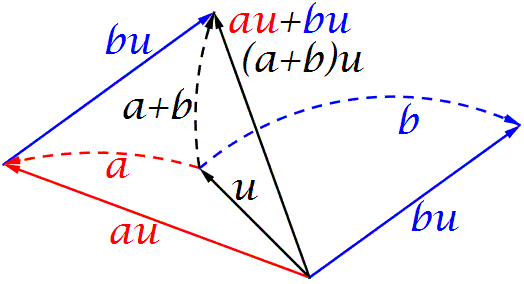
\includegraphics[width=.8\textwidth]{imagenes/imagenes01/T01IM01.png}
	\end{figure}


\section{Ejercicios resueltos}

\begin{ejre} Considera la ley de composición: $a \oplus b=\sqrt[3]{a^3+b^3}$, con $, b\; \in \; \mathbb R$. Demuestra que $(R,\oplus)$ es grupo abeliano.
\end{ejre}

\begin{proofw}\renewcommand{\qedsymbol}{$\diamond$}

\noindent 1) $\oplus$ interna: $a,b\in \mathbb R \to 	a\oplus b=\sqrt[3]{a^3+b^3} \in \mathbb R$ 

\noindent 2) $\oplus$ asociativa: $(a \oplus b) \oplus c = \sqrt[3]{a^3+b^3} \oplus c = \sqrt[3]{(\sqrt[3]{a^3+b^3})^3+c^3}=\sqrt[3]{a^3+b^3+c^3}\; ; \qquad a\oplus(b \oplus c)= a \oplus \sqrt[3]{b^3+c^3} = \sqrt[3]{a^3+(\sqrt[3]{b^3+c^3})^3}= \sqrt[3]{a^3+b^3+c^3}$

\noindent 3) $\oplus$ neutro: $a+e=\sqrt[3]{a^3+e^3}=a=\sqrt[3]{a^3}\to e=0$

\noindent 4) $\oplus$ simétricos: $a\oplus \overline{a}=e \to \sqrt[3]{a^3+{\overline a}^3}=0 \to {\overline{a}}^3=-a^3 \to \overline{a}=-a$

\noindent 5) $\oplus$ conmutativa: $a \oplus b=\sqrt[3]{a^3+b^3}=\sqrt[3]{b^3+a^3}=b \oplus a$

Efectivamente, $\boldsymbol{(R,\oplus)}$ es \textbf{grupo comutativo.}
\end{proofw}

\begin{ejre} Considera las leyes de composición: $a\oplus b=a+b-8; \quad a \otimes b= a+b-ab$, demuestra que $(\mathbb Z, \oplus, \otimes)$ es un anillo.	
\end{ejre}

\begin{proofw}\renewcommand{\qedsymbol}{$\diamond$}

\noindent 1) $\oplus$ interna: 	$a,b\in \mathbb Z \to a+b-8 \in \mathbb Z$

\noindent 2) $\oplus$ asociativa: $(a\oplus b)\oplus c = (a+b-8)\oplus c= (a+b-8)+c-8= a+b+c-16; \qquad a\oplus(b\oplus c)=a\oplus(b+c-8) a+(b+c-8)-8=a+b+c-16$ 

\noindent 3) $\oplus$ neutro: $a\oplus e=a+e-8=a \to e=8$

\noindent 4) $\oplus$ simétrico: $a\oplus \overline{a}=a+\overline{a}-8=e=8 \to \overline{a}=16-a$

\noindent 5) $\oplus$ conmutativa: $a\oplus b=a+b-8 = b+a-8=b\oplus a$

\noindent 6) $\otimes$ interna: $a,b \in \mathbb Z a\otimes b =\to a+b-ab \in \mathbb Z$

\noindent 7) $\otimes$ asociativa:

$(a\otimes b)\otimes c= (a+b-ab)\otimes c =(a+b-ab)+c-(a+b-ab)c=a+b+c-ab-ac-bc+abc$

\centerline{$=$}

$a\otimes(b\otimes c)=a\otimes (b+c-bc)= a+(b+c-bc)-a(b+c-bc)=a+b+c-ab-ac-bc+abc$

\noindent 8) distributiva de $\otimes$ respecto de $\oplus$:

$a\otimes (b\oplus c)=  a\otimes (b+c-8)= a+(b+c-8)-a(b+c-8)=a+b+c-8-ab-ac+8a=9a+b+c-ab-ac-8$

\centerline{$\neq$}

$(a\times b) \oplus (a \otimes c)= (a+b-ab) \oplus (a+c-ac) = (a+b-ab)+(a+c-ac)-8=2a+b+c-ab-ac-8$

No se cumple la propiedad distributiva, luego  $\boldsymbol{(\mathbb Z, \oplus, \otimes)}$ \textbf{no es un anillo}.	

\end{proofw}


\begin{ejre}
	Demuestra que $(\mathbb C,+,\cdot)$, con las leyes usuales de suma y producto de números complejos es un `cuerpo conmutativo'.
\end{ejre}

\begin{proofw}\renewcommand{\qedsymbol}{$\diamond$}
	Recuérdese que un cuerpo es un anillo con elemento inverso para la  segunda ley para todos los elementos de $\mathbb C$ excepto en neutro de la primera ley. Además el cuerpo es conmutativo si lo es la segunda ley. Si antes comprobábamos 8 propiedades, ahora serán 10.
	
	$z\in \mathbb C \; / \; z=a+bi \text{ con } a,b\in \mathbb R; \; i=\sqrt{-1} \notin \mathbb R \; (i^2=-1)$. $a$ es la `parte real' y $b$ la `parte imaginaria', ambas reales.
	
	En lo que sigue, $z_k=a_k+b_k\; i, \; k=\{1,2,3\}; a_k, b_k \in \mathbb R$
	
\noindent 1) $+$ es interna:	 $z_1+z_2=(a_1+b_1 i)+(a_2+b_2 i)=(a_1+a_2)+(b_1+b_2)\;i \; \in \mathbb C$

\noindent 2) $+$ asociativa: $z_1+(z_2+z_3)=(a_1+b_1)\; i + [(a_a+b_2\; i)+ (a_3+b_3)\; i]=\cdots= (a_1+a_2+a_3) + (b_1+b_2+b_3)\; i =\cdots= [(a_1+b_1\; i)+ (a_2+b_2\;i)]+ (a_3+b_3\; i)= (z_1+z_2)+z_3$

\noindent 3) $+$ neutro: $z+e=z \to (a+bi)+ 0 = a+bi \Rightarrow e=0=0+0i$

\noindent 4) $+$ simétrico (opuesto): $z+(-z)=0 \to (a+bi)+ (-z)=0 \Rightarrow -z=-a-bi$

\noindent 5) $+$ conmutativa: $z_1+z_2= (a_1+b_1i)+(a_2+b_2i)=(a_1+a_2)+(b_1+b_2)i=(a_2+a_1)+(b_2+b_1)i=z_2+z_1$

\noindent 6) $\cdot$ interna: $z_1\cdot z_2=(a_1+b_1i)\cdot(a_2+b_2 i)=a_1a_2+a_1b_2i+b_1a_2i+b_1b_2\cancelto{-1}{i^2}=(a_1a_2-b_1b_2)+(a_1b_2+a_2b_1)\;i \in \mathbb C$

\noindent 7) $\cdot$ asociativa:

$z_1\cdot(z_2\cdot z_3)=(a_1+b_1i)\cdot [(a_2a_3-b_2b_3)+(a_2b_3+a_3b_2)\; i]= [a_1(a_2a_3-b_2b_3)-b_1(a_2b_3+a_3b_2)] + [a_1(a_2b_3+a_3b_2)+b_1(a_2a_3-b_2b_3)]\; i \cdots \to$

\centerline{compruébese que son $=$}

$(z_1\cdot z_2)\cdot z_3= [(a_1a_2-b_1b_2)+(a_1b_2+a_2b_1)\;i]\cdot (a_3+b_3i)= \cdots \to $

\noindent 8) $\cdot$ distributiva respecto de $+$:

$z_1\cdot(z_2+z_3)=(a_1+b_1i)\cdot [(a_2+a_3)+(b_2+b_3)\; i] = \cdots \to $

\centerline{compruébese que son $=$}

$(z_1\cdot z_2)+(z_1\cdot z_3)=[(a_1a_2-b_1b_2)+(a_1b_2+a_2b_1)\; i] +  [(a_1a_3-b_1b_3)+(a_1b_3+a_3b_1)\; i] = \cdots \to $ 

\noindent 9) $\cdot$ simétrico (inverso): El neutro en el producto es $1=1+0i; \; z\cdot 1 =(a+bi)(1+0i)=a+bi$

$\forall z\neq 0 \in \mathbb C, \; z=a+bi, \; \exists z^{-1}=\frac 1 z\; / \; z\cdot z^{-1}=1$

En efecto si $z\cdot z^{-1}=1 \to z^{-1}= \frac 1 z = \frac {1}{a+bi}$
\textcolor{gris}{$\cdot \frac {a-bi}{a-bi}$}
$= \frac {a-bi}{a^2-b^2}= \frac {a}{a^2-b^2} + \frac {-b}{a^2+b*2} \; i \in \mathbb C$

\noindent 10) $\cdot$ conmutativa: $z_1\cdot z_2=(a_1+b_1i)\cdot(a_2+b_2 i)=(a_1a_2-b_1b_2)+(a_1b_2+a_2b_1)\;i = (a_2a_1-b_2b_1)+(a_2b_1+a_1b_2)\;i= (a_2+b_2i)\cdot (a_1+b_1i)=z_2\cdot z_1$

\end{proofw}



\begin{myexampleblock}{Comentarios sobre los números complejos.}

\small{El nombre escogido, `números complejos',  para estos números tiene lo suyo, pero ... sigamos adelante.}

\vspace{2mm}
\small{Estos extraños números surgen de la mano de Cardano y Tartaglia en el s. XVI, cuando intentaban resolver ecuaciones de tercer grado. Se dieron cuenta que necesitaba considerar las raíces cuadradas de números negativos, así, p.e., para calcular $\sqrt{-25}$ hacían lo siguiente: $\sqrt{-25} = \sqrt{ 25 \cdot (-1)} = \pm 5 \; \sqrt{-1}$}


\vspace{2mm}
\small{En el s. XVII, Leibniz considera a la $\sqrt{-1}$ como una especie de `anfibio entre el ser y la nada'. Los matemáticos y físicos de la época usan estos números pero con desconfianza.}


\vspace{2mm}
\small{Euler, en el s. XVIII bautiza a $\sqrt{-1}$ como $i$ (de número imaginario). Ahora, las raíces de números negativos son algo tan sencillo como $\sqrt{-4}=\pm 2\;i$}


\vspace{2mm}
\small{A finales del s. XVIII, Euler demuestra su famoso TEOREMA FUNDAMENTAL DEL ÁLGEBRA, que asegura que todo polinomio de grado $n$ tiene, exactamente, $n$-raíces (considerando la multiplicidad y estas imaginarias).  Así, p.e., la ecuación                 $x^2-4x+13=0$ tiene por soluciones  $2+3i$  y  $2-3i$.}


\vspace{2mm}
\small{A partir del s. XIX, Gauss logra la representación gráfica de estos números complejos y su interpretación geométrica. Desde entonces son aceptados sin reservas.}


\vspace{2mm}
\small{s. XXI. La aplicación de los números complejos está presente en muchos apartados de las ciencias.}

\vspace{2mm}
\small{--- En electrónica la ley de ohm ($IR=V$) para corriente alterna necesita de los números complejos: $IZ=V; \; Z=R+iX$  ($Z$ impedancia, tiene parte real o resistiva $R$ y parte imaginaria o reactancia $X$)}

\vspace{2mm}
\small{También se usan los números complejo en electromagnetismo (las ondas e.m. son complejas) y en física cuántica (la amplitud de probabilidad es compleja, su cuadrado es lo observable).}


\vspace{2mm}
\small{--- En la teoría especial de la relatividad se reformula el espacio-tiempo 4-dimensional de Minkowski en el que el tiempo es una componente más, imaginaria. En palabras de Minkowski, en 1908, \textbf{``las ideas que sobre el espacio-tiempo quiero mostrarles hoy descansan en el suelo firme de la física experimental, en la cual yace su fuerza. Son ideas radicales. Por lo tanto, el espacio y el tiempo, por separado, están destinados a desvanecerse entre las sombras y tan solo una unión de ambos puede representar la realidad.''}}


\vspace{2mm}
\small{--- ?`Qué no decir de los fractales?. En 1977 Benoit Mandelbrot publica `la geometría fractal de la naturaleza', regida por números complejos ($\; z_{n+1}=z_n^2+c$, `conjunto de Mandelbrot').}


\vspace{2mm}
\centerline{La ecuación más bella:    $\boxed{\;\boldsymbol{ e^ {i\cdot \pi}  + 1 = 0} \;} $}

\end{myexampleblock}

\vspace{5mm}
	\begin{figure}[H]
		\centering
		
\includegraphics[width=1\textwidth]{imagenes/imagenes01/T01IM07.png}
	\end{figure}




	%\begin{figure}[H]
		%\centering
		%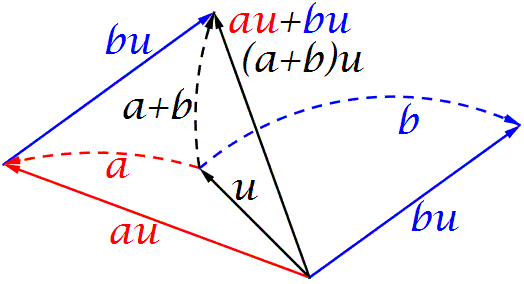
\includegraphics[width=0.5\textwidth]{imagenes/imagenes01/T01IM01.png}
		%\caption{Los dos problemas clásicos del cálculo: trazado de tangentes y áreas bajo curvas.}
	%\end{figure}
		
%varios párrafos encuadrados - explicaciones ad hoc
%\centering{
%\fbox{
%\parbox{0.95\textwidth}{
%varios
%
%$parrafos
%
%dentro
%}
%}
%}
% \justify


%\rotatebox{180}{\leftline{\textcolor{gris}{tararí}}}.

\chapter{Sistemas de ecuaciones lineales: método de Gauss}
\chaptermark{S.E.L.: MÉTODO DE GAUSS}	

\section[Sistemas de dos ecuaciones lineales con dos incógnitas]{Sistemas de dos ecuaciones lineales con dos incógnitas}\sectionmark{Sistemas 2ecc-2incog}
\sectionmark{Sistemas 2ecc-2incog}
\begin{defi}
Una `ecuación lineal' con dos incógnitas es una relación de la forma: $ax+by=c$, con $a,b,c \in \mathbb R$. $x$ e $y$ son las incógnitas	.
Cualquier par de valores $(\alpha, \beta)$ que verifiquen la ecuación se llaman `solución' de la misma.
\end{defi}
\vspace{-3mm}
\noindent \small{--- Cualquier ecuación lineal con dos incógnitas, $ax+by=c$, admite siempre infinitas soluciones. Hay que dar valor a una incógnita y calcular el valor correspondiente en la otra.}

\noindent \small{--- Interpretación geométrica: si representamos en el plano todas las infinitas soluciones de cualquier ecuación lineal con dos incógnitas, $ax+by=c$, obtenemos una `recta' en el plano.}

\small{Vamos a empezar considerando sistemas de \textbf{2} ecuaciones lineales con \textbf{2} incógnitas. 
$\begin{cases}a_1x+b_1y=c_1\\a_2x+b_2y=c_2\end{cases}; \; a_i,b_i$ son los coeficientes y $c_i$ los términos independientes ($i=\{1,2\}$)}
\begin{defi}
Según sean las soluciones del sistema de ecuaciones lineales con dos incógnitas, éstos se clasifican en:	
\begin{enumerate}
\item \small{SISTEMA COMPATIBLE DETERMINADO (SCD): Solución única.}

\small{ejemplo: $\begin{cases} x-y=-3 \\2x+y=6 \end{cases} $
$\to \quad  \begin{matrix} 
\text{ sumando: } 
\\ 3x=3\;\to \;    \boldsymbol{x=1; \; y=4}
\end{matrix}$}

\small{Interpretación geométrica: las dos rectas que forman el sistema son secantes, ($r\cap s$), se cortan en un punto, el $(1,4)$.}
\item \small{SISTEMA COMPATIBLE INDETERMINADO (SCI): Infinitas soluciones.}

\small{ejemplo: $\begin{cases} x-y=-3 \\2x-2y=-6 \end{cases} \to \; \; \begin{matrix}  (1^a ec)(2)-(2^a ec) \\  0x=0;\;   \boldsymbol{x=\lambda} \to  \boldsymbol{y=3+\lambda} \\ \forall \lambda \in \mathbb R; \; \infty \text{ soluciones}\end{matrix}$	}

\small{Interpretación geométrica: las dos rectas que forman el sistema son coincidentes ($r \equiv s$), tienen todos ($\infty$) puntos en común.}
\item \small{SISTEMA INCOMPATIBLE (SI): No hay ninguna solución.}

\small{ejemplo: $\begin{cases} x-y=-3 \\2x-2y=5 \end{cases} \to \; \; \begin{matrix}  (1^a ec)(2)-(2^a ec) \\  0x=-8;\;   \boldsymbol{\nexists \; x}\; \to  \boldsymbol{\nexists \;  y} \end{matrix}$}	

\small{Interpretación geométrica: las dos rectas que forman el sistema son paralelas ($r \parallel s$), no tienen ningún punto en común.}
\end{enumerate}
\end{defi}

	\begin{figure}[H]
		\centering
		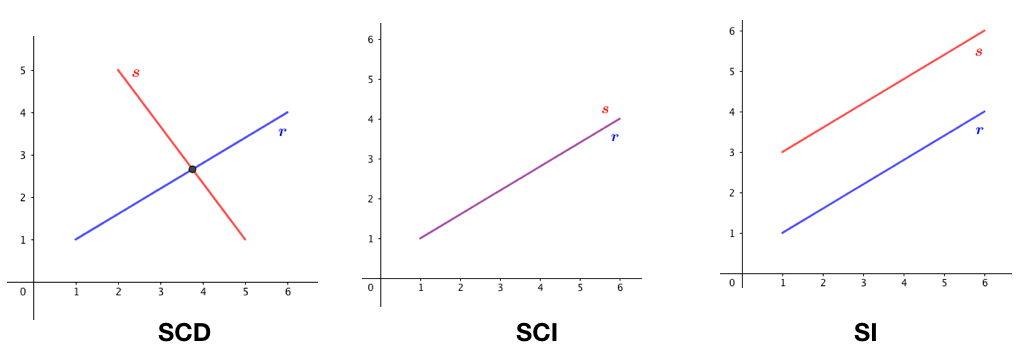
\includegraphics[width=1\textwidth]{imagenes/imagenes01/T01IM02.png}
	\end{figure}


\noindent \textbf{Forma matricial de un sistema de dos ecuaciones con dos incógnitas}
\vspace{4mm}

Aunque dedicaremos en un próximo capítulo a las matrices, de momento nos bastará considerar una matriz como un rectángulo que contiene números. Así, un Sistema de Ecuaciones Lineales (en adelante un SEL) lo podremos escribir, escribiendo en cada fila solamente los coeficientes de las ecuaciones y, a la derecha, separada por una barra vertical, |, los términos independientes. En la segunda fila se escribirán los coeficientes de la segunda ecuación y, a la derecha, su término independiente. En este caso usaremos una matriz de dos filas (ecuaciones) con tres columnas (dos para os coeficientes de las incógnitas  y la tercera columna para los términos independientes).

\vspace{4mm} \centerline{$\boxed{\; \begin{cases}a_1x+b_1y=c_1\\a_2x+b_2=c_2\end{cases} \Leftrightarrow 
\left[
\begin{matrix}
\; a_1&b_1\\
\; a_2&b_2	
\end{matrix}
\right|
\left.
\begin{matrix}
c_1\\c_2	
\end{matrix}
\right]\;} \; $
$\begin{matrix}\text{ Forma matricial de un S }\\\text{de dos E L con dos incog.}\end{matrix}$}

\vspace{4mm} $a_1, b_1, a_2, b_2$ son los coeficientes; $c_1, c_2$ son los términos independientes.

\section[Sistemas de Ecuaciones Lineales]{Sistemas de Ecuaciones Lineales}\sectionmark{SEL}
\sectionmark{SEL}

\begin{defi}
Se llama `Sistema de m-Ecuaciones Lineales con n-incógnitas' (SEL) a todo conjunto de relaciones de la forma:

\vspace{4mm}

\centerline{$\boxed{\; \begin{cases}
\;\; a_{11} x_1 + a_{12} x_2 + \cdots + a_{1j} x_j+ \cdots + a_{1n} x_n & = b_1\; \\
\;\; a_{21} x_1 + a_{22} x_2 + \cdots + a_{2j} x_j+ \cdots + a_{2n} x_n & = b_2\; \\
\;\; \cdots \quad \cdots \quad \cdots 	\quad \cdots \quad \cdots \quad \cdots \quad \cdots \quad \cdots & \cdots \\
\;\; a_{i1} x_1 + a_{i2} x_2 + \cdots + a_{ij} x_j+ \cdots + a_{in} x_n & = b_i\; \\
\;\; \cdots \quad \cdots \quad \cdots 	\quad \cdots \quad \cdots \quad \cdots \quad \cdots \quad \cdots & \cdots \\
\;\; a_{m1} x_1 + a_{m2} x_2 + \cdots + a_{mj} x_j+ \cdots + a_{mn} x_n & = b_m\; \\
\end{cases}}$}	
\end{defi}

\vspace{4mm} 

La primera fila son los coeficientes de las n-incógnitas y el término independiente de la primera ecuación. La segunda fila, la segunda ecuación, ... En la primera columna aparecen los coeficientes de la primera incógnita, en la segunda columna los coeficientes de la segunda incógnita, ... En la columna m+1 aparecen los términos independientes de las m-ecuaciones. Así, $a_{ij}$ es el coeficiente de la ecuación-i que acompaña a la incógnita-j.


\begin{myblock}{Forma matricial para representar un SEL}
\centerline{
$\left[ \begin{matrix}
\; a_{11} & a_{12} & \cdots & a_{1j} & \cdots & a_{1n} \;  \\
\; a_{21} & a_{22} & \cdots & a_{2j} & \cdots & a_{2n} \;  \\
\; \vdots & \vdots & \ddots & \vdots & \ddots & \cdots \;  \\
\; a_{i1} & a_{i2} & \cdots & a_{ij} & \cdots & a_{in} \;  \\
\; \vdots & \vdots & \ddots & \vdots & \ddots & \cdots \;  \\
\; a_{m1} & a_{m2} & \cdots & a_{mj} & \cdots & a_{mn} \;  
\end{matrix} \right.$
$\left| \begin{matrix}
\; b_1 \; \\
\; b_2 \;  \\
\; \vdots \; \\
\; b_i \; \\
\; \vdots \; \\
\; b_m \; 	
\end{matrix} \right]$
}
\end{myblock}


De nuevo, para cada $a_{ij}$, el subíndice-i hace referencia a la ecuación-i y el subíndice-j a la incógnita-j: $\; 1\le i\le m;\;$, m ecuaciones ; $ \; 1\le j \le n \;$, n-incógnitas.

\begin{defi}
Decimos que la n-tupla \textcolor{gris}{(conjunto de n números ordenados)} de números reales $(\alpha_1, \alpha_2, \alpha_3, \cdots, \alpha_n)$ son `solución' del SEL si sustituidas en él se satisfacen todas sus ecuaciones. 	
\end{defi}

\begin{defi}.
\begin{myblock}{Atendiendo a las soluciones, un SEL puede ser:}
$\begin{cases}
\text{COMPATIBLE (con solución)	} \; \; 	\to \; \begin{cases}
\text{DETERMINADO (Sol.única)} \\
\text{INDETREMINADO } (\infty \text{ sol.})
\end{cases}
\\
\text{INCOMPATIBLE (sin solución)} 	 \; \begin{matrix}
\text{ } \\
\text{}
\end{matrix}

\end{cases}$
\end{myblock}	
\end{defi}
\begin{defi}
	'`Resolver' un SEL es encontrar todas sus soluciones o advertir de que el sistema carece de soluciones.
\end{defi}

\section{Sistemas equivalentes}
\begin{defi}
Dos sistemas de ecuaciones lineales con el mismo número de incógnitas (aunque no tengan el mismo número de ecuaciones) se dice que son `equivalentes' si tienen las mismas soluciones, es decir, cualquier solución del primer sistema también lo es del segundo y viceversa.	
\end{defi}
\begin{teor}
Las siguientes transformaciones elementales realizadas a un SEL dan lugar a otro equivalente:

\begin{itemize}
\item Cambiar de orden las ecuaciones del sistema.
\item Multiplicar toda la ecuación (los dos miembros) por un número distinto de cero.
\item Sustituir una ecuación del sistema por ella misma más otra cualquiera multiplicada por un número cualquiera.
\item Sustituir una ecuación del sistema por ella misma multiplicada por un `numero distinto de cero' más otras ecuaciones multiplicadas por otros números. \textcolor{gris}{!`Ojo!, la ecuación a sustituir no puede estar multiplicada por cero, sería como cargarse una ecuación del sistema.}	
\end{itemize}
	
\end{teor}


\section[Resolución de SEL: Método de Gauss]{Resolución de SEL: Método de Gauss}\sectionmark{Método de Gauss}
\sectionmark{Método de Gauss}


El método de Gauss consiste en aplicar transformaciones a las ecuaciones (filas de números en la representación matricial) hasta obtener un sistema “triangular” (todos los coeficientes por debajo de la diagonal son cero) y, entonces, despejar en cascada (de abajo hacia arriba). Si nos aparece una trivialidad, $0=0$, se tacha y se prescinde de esa fila o ecuación (no aporta ninguna información al sistema); si llegamos a una incongruencia (incompatibilidad) $3=0$, p.e., tenemos un SI (sin solución). 

Este método está formado por varios pasos (m-1 pasos de las m-1 ecuaciones en que hay que buscar ceros por debajo de la diagonal): 

--- el primer paso consiste en combinar cada una de las ecuaciones $2, 3, \cdots, m$ con la ecuación $1$ para que todos sus primeros coeficientes sean cero ($a_{21}=a_{31}=\cdots=a_{m1}=0)$.

--- el segundo paso consiste en hacer que por debajo de la segunda fila, todos los segundos coeficientes del resto de ecuaciones sean cero, combinando cada ecuación $3, 4, \cdots , ,$ con la $2$ para conseguir que $a_{32}=a_{42}=\cdots=a_{m2}=0$.

--- y así hasta conseguir triangularizar la matriz, que por debajo de la diagonal todos los elementos sean ceros. 
				
	\begin{figure}[H]
		\centering
		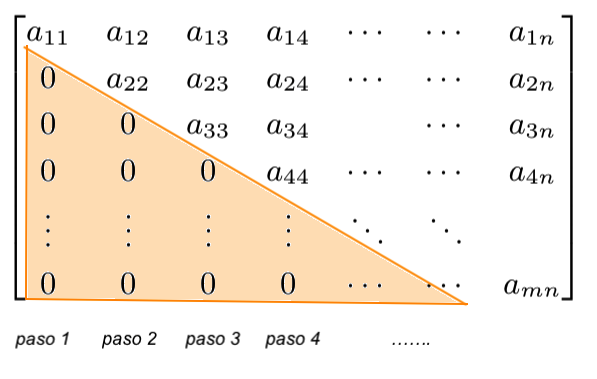
\includegraphics[width=0.7\textwidth]{imagenes/imagenes01/T01IM05.png}
	\end{figure}				
				
Cuando se llega a una ecuación con más de una incógnita se elige una de ellas y a las otras se les da valores arbitrarios (parámetros $\lambda, \mu, ...$) y se sigue despejando en función de éstos. Para ello:
				
\begin{teor}{Transformaciones de Gauss:} En la representación matricial de un SEL está permitido (da lugar a otra ecuación equivalente):
		
	\hspace{3mm} \colorbox{LightYellow}{* multiplicar una ecuación por un número distinto de cero.}
		
	\hspace{3mm}  \colorbox{LightYellow}{* Sustituir una ecuación por ella misma más otra  multiplicada} 
	
	\hspace{3mm} \colorbox{LightYellow}{ por un número.}
		
\noindent !`ASTUCIA!: se puede cambiar el orden de las ecuaciones y las incógnitas (advirtiéndolo en este último caso). Lo más conveniente es que el número con el que combinar, `pivote', sea $1$ ò $-1$, si es posible. En caso de que el coeficiente con el que pivotar sea cero, o bien cambiamos de orden las ecuaciones o sustituimos ésta por una combinación de ella con alguna otra de modo que el pivote sea distinto de cero.
\end{teor}



A continuación veremos unos ejemplos de resolución de sistemas de ecuaciones lineales por el método de Gauss.

\begin{ejem}.

$\begin{cases}
x-2y-2z&=-3\\2x-3y+4z&=4\\5x-y+3z&=16	
\end{cases} \to \left[ \begin{matrix}
 1&-2&-2\\2&-3&4\\5&-1&3	
 \end{matrix}\right. 
 \left| \begin{matrix}
 -3\\4\\16	
 \end{matrix}\right] \; \underrightarrow {(1*)} \;  
 \left[ \begin{matrix}
 1&-2&-2\\0&1&8\\0&9&13	
 \end{matrix}\right. 
 \left| \begin{matrix}
 -3\\10\\31	
 \end{matrix}\right] \; \underrightarrow {(2*)} \; $
 
 $
  \left[ \begin{matrix}
 1&-2&-2\\0&1&8\\0&0&-59	
 \end{matrix}\right. 
 \left| \begin{matrix}
 -3\\10\\-59	
 \end{matrix}\right] \;  \Rightarrow  \; \begin{cases}
 x-2y-2z=-3\\ y+8z=10\\-59z=-59	
 \end{cases}$

En el paso (1*) --primer paso del método de Gauss-- hemos combinado las ecuaciones segunda y tercera con la primera para conseguir los dos ceros de la primera columna ($2^a\to 2^a-2\cdot 1^a; \; \; 3^a\to 3^a-5\cdot 1^a$). En el paso (2*) --segundo paso del método de Gauss-- combinamos la tercera ecuación con la segunda para conseguir el cero de la tercera columna \textcolor{gris}{(ojo, combinamos 3$^a$ con 2$^a$ , no con 1$^a$, que desharíamos el cero anteriormente conseguido)}, la combinación elegida en este caso ha sido $3^a \to 3^a - 9\cdot 2^a$. \textcolor{gris}{Estos pasos no será necesarios explicarlos así como tampoco lo será reescribir el sistema de ecuaciones escalonado al que llegamos}. Con ello hemos conseguid un sistema `escalonado' y (sin necesidad de volver a escribir el sistema de ecuaciones lineales obtenido) nos ponemos a despejar en `cascada', de abajo hacia arriba: 

Leyendo la última ecuación: $[\; 0 \quad 0 \quad -59 \;\;  | \; \; -59 ] \to  -59z=-59 \Rightarrow \boldsymbol{z=1}$ 

Subimos un peldaño en la cascada y, con el valor encontrado para $x$, leemos la segunda ecuación: $[\; 0\quad 1 \quad 8 \; \; | \; \; 10] \to y+8z=10; \; y+8\cdot 1=10 \Rightarrow \boldsymbol{y=2}$

Por último, subimos a la primera ecuación y leemos: $[\; 1\quad -2\quad -2 \; \; | \; \; -3 ] \to x-2y-2z=-3 ; \; x -2\cdot 2-2\cdot 1=-3 ; \; x-4-2=-3 \rightarrow \boldsymbol{x=3}$

Solución única: $\boldsymbol{x=3;\;  y=2; \; z=1}$, \textbf{solución única}, \textbf{SDC} (sistema compatible y determinado).
\end{ejem}

\begin{ejem}.

$\begin{cases}
x-y+3z&=4\\2x-y-z&=6\\3x-2y+2z&=10	
\end{cases} \to \left[ \begin{matrix}
 1&-1&3\\2&-1&-1\\3&-2&2	
 \end{matrix}\right. 
 \left| \begin{matrix}
 4\\6\\10	
 \end{matrix}\right] \; \underrightarrow {(1*)} \;  
 \left[ \begin{matrix}
 1&-1&3\\0&1&-7\\0&1&-7	
 \end{matrix}\right. 
 \left| \begin{matrix}
 4\\-2\\-2	
 \end{matrix}\right] \; \underrightarrow {(2*)} \; $
 
 $
  \left[ \begin{matrix}
 1&-1&3\\0&1&-7\\ 0&0&0
 \end{matrix}\right. 
 \left| \begin{matrix}
 4\\-2\\0	
 \end{matrix}\right] \;  \Rightarrow  \; \begin{cases}
 x-y+3z=4\\ y-7z=-2\\0z=0	
 \end{cases}$
 
  \textcolor{gris}{$1*)\;\; 2ec \to 2ec  -  2\cdot 1ec; \; \; 3ec\to 3ec - 5\cdot 1ec; \quad 2*)\; \; 3ec \to 3ec  -  2ec $}


La última ecuación: $[\; 0\quad 0\quad 0 \; \; |\;\;  0\;]$ es lo que en matemáticas llamamos una `trivialidad' ($0\cdot z=0$), no aporta ninguna información y la eliminamos del sistema:

$  \left[ \begin{matrix}
 1&-1&3\\0&1&-7\\ \text{\textst{ 0 }} & \text{\textst{ 0 }} & \text{\textst{ 0 }}
 \end{matrix}\right. 
 \left| \begin{matrix}
 4\\-2\\ \text{\textst{ 0 }}	
 \end{matrix}\right] $


Leyendo ahora la última ecuación que ha quedado: $y-7z=-2$. Para resolver una ecuación con más de una incógnita, hay que elegir una de ellas, la $y$ por ejemplo y dar valores a las otras, la $z$ en este caso. En el problema que nos ocupa (método de Gauss para resolver SEL) lo que haremos es `parametrizar' las otras incógnita, $z$ en el ejemplo, del siguiente modo: $\;z=\lambda\; \; \forall \lambda \in \mathbb R$ e ir despejando el resto de incógnitas en función de estos parámetros:



$\;z=\lambda\; \; \forall \lambda \in \mathbb R \to \; $, última ecuación $\; y-7z=-2; \; y-7\lambda=-2 \Rightarrow y=-2+7\lambda\; $. Subimos un peldaño y vamos a la primera ecuación: $\; x-y+3z=4 \to x-(-2+7\lambda)+3\lambda=4 \Rightarrow x=2+4\lambda$



Las soluciones son: $\boldsymbol{\; x=2+4\lambda; \; \; y=-2+7\lambda; \; \; z=\lambda \;} $, como esto es  $\boldsymbol{\; \forall \lambda \in \mathbb R\;}$, tenemos \textbf{infinitas soluciones: SCI} (Sistema compatible Indeterminado)

Por ejemplo, si $\lambda=0 \to x=2; \; y=-2; \; z=0$ es una solución del sistema, la terna de números $(2,-2,0)$, en ese orden, son verifican todas las ecuaciones del sistema (x el primer número, y el segundo y z el tercero, de la terna). Para, p.e., $\lambda=-2 \to (-6,-16,-2)$, también lo es y así, como valores de $\lambda \in \mathbb R$ hay $\infty$, se pueden obtener las infinitas soluciones del mismo.

?`Es $(2,3,-1)$ solución del sistema?. Si lo fuese, $z=-1=\lambda \to x=-2\neq 2; \; y=-9\neq 3$. No, $(2,3,-1)$  no es solución del sistema.

?`Es $(32, 47, 7) $ solución del sistema? $\to z=7=\lambda \to x=32\; \; y=47$. Sí lo es.

?`¿Que deben valer $m$ y $n$ para que $(4,m,n)$ sea solución del sistema? Dicho de otro modo, Si $x=4$ es una de las soluciones del sistema, ?`qué vales las otras? Como $x=2+4\lambda=4 \to \lambda = \frac 1 /2 \Rightarrow y=-2+\frac 7 2=\frac 3 2; \; z=\frac 1 2$.
\end{ejem}

\begin{ejem}.

$\begin{cases}
2x-y+3z&=6\\4x-2y+6z&=9\\x-y+z&=3	
\end{cases} \to \left[ \begin{matrix}
 2&-1&3\\4&-2&6\\1&-1&1	
 \end{matrix}\right. 
 \left| \begin{matrix}
 \; 6\\\; 9\\\; 3	
 \end{matrix}\right] \;\underrightarrow {(1*)} \;  
 \left[ \begin{matrix}
 1&-1&1\\2&-1&3\\4&-2&6	
 \end{matrix}\right. 
 \left| \begin{matrix}
 \; 3\\\; 6\\\; 9		
 \end{matrix}\right] \underrightarrow {(2*)} \; $
 
 $ 
 \left[ \begin{matrix}
 1&-1&3\\0&1&1\\0&2&2	
 \end{matrix}\right. 
 \left| \begin{matrix}
 3\\0\\-3	
 \end{matrix}\right] \; \underrightarrow {(3*)} \; 
 \left[ \begin{matrix}
 1&-1&1\\0&1&1\\ 0&0&0
 \end{matrix}\right. 
 \left| \begin{matrix}
 3\\0\\-3	
 \end{matrix}\right] \;  \Rightarrow  \; \begin{cases}
 x-y+z=3\\ y+z=0\\0z=-3	
 \end{cases}$

 
 \textcolor{gris}{$1)\; \text {reorganización de ecuaciones, ponemos la tercera en primer lugar };$}
 
 \textcolor{gris}{$ 2) \; 2ec \to 2ec-2\; 1ec  ; \; \; 3ec \to 3e -4\; 1ec; $}
 
  \textcolor{gris}{ $  3) \; 3ec \to 3ec-2\; 2ec $}
 
 
 Eliminadas las trivialidades (en este caso no hay), leyendo la última fila del método de Gauss: $[\;0\quad 0\quad 0 \; \; | \; \; -3 \; ]$, tenemos que $0\cdot z=-3; \; \nexists \;z\in \mathbb R$, no hay solución para $z$, ni para $y$ ni para $x$.

  El \textbf{sistema no tiene solución}, es un \textbf{SI} (sistema incompatible).
\end{ejem}



\section[Discusión de sistemas por el método de Gauss]{Discusión de sistemas por el método de Gauss}\sectionmark{Discusión de sistemas}
\sectionmark{Discusión de sistemas}

En ocasiones se nos presentan problemas de SEL dependientes de un parámetro. Según los distintos valores que tome el parámetro el sistema puede tener o no soluciones y, en el caso de tenerlas, éstas pueden ser únicas (una para cada incógnita) o ser infinitas (dependiendo de un parámetro). 

\begin{defi}
`Discutir' un SEL en función de uno o varios parámetros es encontrar el valor de estos para los cuales el sistema es compatible y resolverlo en los casos de compatibilidad.

Para ello usaremos el método de Gauss (hay que ir con cuidado por si  hay que cambiar una ecuación por ella misma multiplicada por $k$ con una combinación de las demás, !` $k\neq 0$ !, de lo contrario nos cargaríamos una ecuación.

El análisis de la solución del sistema escalonado nos determinarán los valores del/los parámetro/s para que tenga solución
\end{defi}

 Como astucia para la discusión de SEL por Gauss es conveniente tomar el parámetro cuanto más tarde, mejor.

El método de Gauss no es el procedimiento más adecuado para la discusión de SEL dependientes de parámetros, para ello usaremos el `Teorema de Rouché-Froebenius', que desarrollaremos en temas posteriores.

\begin{ejem} Discutir el siguiente sistema y resolverlo en los casos de compatibilidad.
$\begin{cases} x+y+az&=1\\x+ay+z&=1\\ax+y+z&=1\end{cases} \longrightarrow $
$\left[ \begin{matrix}
 1 & 1 & a \\ 1 & a & 1\\ a & 1 & 1 
 \end{matrix}\right. 
 \left| \begin{matrix}
  1 \\ 1 \\ 1 
 \end{matrix}\right]  \to$
$\left[ \begin{matrix}
 1 & 1 & a \\ 0 & a-1 & 1-a \\ 0 & 1-a & 1-a^2
 \end{matrix}\right. 
 \left| \begin{matrix}
  1 \\ 0 \\ 1-a 
 \end{matrix}\right] \to $	
$\left[ \begin{matrix}
 1 & 1 & a \\ 0 & a-1 & 1-a \\ 0 & 0 & 2-a-a^2
 \end{matrix}\right. 
 \left| \begin{matrix}
  1 \\ 0 \\ 1-a 
 \end{matrix}\right] \to 
 a^2-a-2=0 \Rightarrow \begin{cases} a=1 \\ a=-2\end{cases}$
 
 Tenemos que distinguir tres casos: $a=1$; $a=-2$ y $a\neq 1 \; \wedge \; x\neq -2$:
 
 ---caso: $\boldsymbol{a\neq 1 \; \wedge \; x\neq -2} \to \boldsymbol{SCD}, \text{ solución única }: \boldsymbol{x=y=z=\frac 1 {a+2}}$
 
 \textcolor{gris}{Ya que $2-a-a^2=-(a-1)(a+2)=(1-a)(a+2),$ ambos factores distintos de cero, por ello: $(1-a)(a+2)z=1-a \to z=\frac 1 {a+2}$ y resolviendo en cascada se encuentran las otras soluciones.}
 
 --- caso: $a=1$: (particularizando) $\left[ \begin{matrix}
 1 & 1 & 1 \\  \text{\textst{ 0 }} &  \text{\textst{ 0 }} &  \text{\textst{ 0 }} \\  \text{\textst{ 0 }} &  \text{\textst{ 0 }} &  \text{\textst{ 0 }}
 \end{matrix}\right. 
 \left| \begin{matrix}
  1 \\  \text{\textst{ 0 }} \\  \text{\textst{ 0 }} 
 \end{matrix}\right].\;$ Eliminando las trivialidades: $x+y+z=1$ una ecuación y 3 incógnitas. Daremos valores arbitrarios (parámetros) a dos de ellas y despejamos la tercera:
 
 Sea $z=\lambda; \; \forall \lambda \in \mathbb R; \; \; y=\mu; \; \forall \mu \in \mathbb R\; \to x+\mu+\lambda=1 \Rightarrow x=1-\mu-\lambda$
 
 En el caso $\boldsymbol{a=1}$, soluciones: $\boldsymbol{x=1-\mu-\lambda; \; y=\mu; \; z=\lambda; \; \; \forall \lambda, \mu \in \mathbb R}$. Abreviadamente hay quien lo escribe así: $(1-\mu-\lambda, \mu, \lambda)$. Tenemos un \textbf{SCI} (infinitas soluciones).
 
 --- caso: $\boldsymbol{a=-2}$: (particularizando) $\left[ \begin{matrix}
 1 & 1 & -2 \\ 0 & -2 & 3 \\ 0 & 0 & 0
 \end{matrix}\right. 
 \left| \begin{matrix}
  1 \\ 0 \\ 3 
 \end{matrix}\right]\; $ 
 
 La tercera ecuación muestra una incompatibilidad: $0=3$ ó $0z=3 \to \nexists z, \nexists y, \nexists x$, tenemos un\textbf{SI}, es decir, \textbf{el sistema no tiene solución}.
 
\end{ejem}



\section{Sistemas homogéneos}

\begin{defi}
Decimos que un SEL es `homogéneo' si todos sus términos independientes son cero.


	
\end{defi}
\begin{teor}Todos los `sistemas homogéneos son compatibles'.	
\end{teor}

\centerline{$\boxed{\; \begin{cases}
\;\; a_{11} x_1 + a_{12} x_2 + \cdots + a_{1j} x_j+ \cdots + a_{1n} x_n & = 0\; \\
\;\; a_{21} x_1 + a_{22} x_2 + \cdots + a_{2j} x_j+ \cdots + a_{2n} x_n & = 0\; \\
\;\; \cdots \quad \cdots \quad \cdots 	\quad \cdots \quad \cdots \quad \cdots \quad \cdots \quad \cdots & \cdots \\
\;\; a_{i1} x_1 + a_{i2} x_2 + \cdots + a_{ij} x_j+ \cdots + a_{in} x_n & = 0\; \\
\;\; \cdots \quad \cdots \quad \cdots 	\quad \cdots \quad \cdots \quad \cdots \quad \cdots \quad \cdots & \cdots \\
\;\; a_{m1} x_1 + a_{m2} x_2 + \cdots + a_{mj} x_j+ \cdots + a_{mn} x_n & = 0\; \\
\end{cases}}$}

\begin{proof}
Evidentemente, todo sistema homogéneo admite la solución llamada `trivial' en que todos las incógnitas toman el valor $0$. No hay más que sustituir todas las $x_i$ por $0$ en el sistema homogéneo para convencernos de que se verifican todas sus ecuaciones. Pero puede que hayan otras soluciones, además de la trivial (evidentemente) que también verifiquen el sistema, por eso el teorema asegura que todo sistema homogéneo es COMPATIBLE, pudiendo ser Determinado o Indeterminado (infinitas soluciones, entre ellas estará la trivial). Como se verá en os ejemplos siguientes	eso se determina en la resolución de los mismos.
\end{proof}
\begin{defi}
Llamamos `solución trivial' de un SEL homogéneo a aquella en que el valor de todas sus incógnitas es cero: $x_1=x_2=\cdots=x_n=0$	
\end{defi}

\begin{ejem}
	$\begin{cases} x+2y-3z &=0 \\ x-y+z &=0 \\ 2x-z&=0 \end{cases} \to$
$\left[ \begin{matrix}
  1 & 2 & -3 \\ 1 & -1 & 1 \\ 2 & 0 & -1 
 \end{matrix}\right. 
 \left| \begin{matrix}
  0 \\ 0 \\ 0 
 \end{matrix}\right] \to $
 $\left[ \begin{matrix}
 1  & 2 & -3 \\ 0 & 3 & -4 \\ 0 & 4 & -5 
 \end{matrix}\right. 
 \left| \begin{matrix}
  0 \\ 0 \\ 0 
 \end{matrix}\right] \to $
$\left[ \begin{matrix}
 1  & 2 & -3 \\ 0 & 3 & -4 \\ 0 & 0 & 1 
 \end{matrix}\right. 
 \left| \begin{matrix}
  0 \\ 0 \\ 0 
 \end{matrix}\right] \to z=0; \; 3y-4(0)=0 \to y=0; \; x+2(0)-3(0)=0 \to x=0$
 
 Hemos obtenido la solución única $\boldsymbol{x=y=z=0}$, la solución trivial. Los sistemas \textbf{SCD} homogéneos solo tiene una solución por ser compatibles y siempre admiten la solución trivial por ser homogéneos: Conclusión: \textit{`la única solución de un SCD homogéneo es la solución trivial'}
\end{ejem}

\begin{ejem}
$\begin{cases}x+y-z=0\\12x-3y-2z=0\\-2x+13y-8z=0\end{cases} \to$
$\left[ \begin{matrix}
  1 & 1 & -1 \\ 12 & -3 & -2 \\ -2 & 13 & 8 
 \end{matrix}\right. 
 \left| \begin{matrix}
  0 \\ 0 \\ 0 
 \end{matrix}\right] \to $	
 
 
 $\left[ \begin{matrix}
  1 & 1 & -1 \\ 0 & -15 & 10 \\ 0 & 15 & -10 
 \end{matrix}\right. 
 \left| \begin{matrix}
  0 \\ 0 \\ 0 
 \end{matrix}\right] \to $
 $\left[ \begin{matrix}
  1 & 1 & -1 \\ 0 & -15 & 10 \\ \text{\textst{ 0 }}  & \text{\textst{ 0 }}  & \text{\textst{ 0 }}  
 \end{matrix}\right. 
 \left| \begin{matrix}
  0 \\ 0 \\ \text{\textst{ 0 }}  
 \end{matrix}\right] \to $
 
 Eliminada la trivialidad, la última ecuación dice: $-15y+10z=0; \; z=\lambda, \; \forall \lambda \in \mathbb R \to y=2\	lambda /3; \; x=\lambda /3; \; \; SCI$
 
 Hemos obtenido un SCI (sistema compatible indeterminado, infinitas soluciones): $\boldsymbol{x=\frac {\lambda} 3; \; y=2 \frac {\lambda} 3; \; z= \lambda \; \; \forall \lambda \; \in \mathbb R}$. Pero tenemos un sistema homogéneo, entre estas soluciones también debe estar la solución trivial $x=y=z=0$. En efecto, basta con tomar $\lambda=0$.
\end{ejem}


\begin{ejem} Discusión de un sistema homogéneo.

$\begin{cases}2x-y+z&=0\\x+2y-3z&=0\\3x-4y-kz&=0\end{cases} \to $
$\left[ \begin{matrix}
  2 & -1 & 1 \\ 1 & 2 & -3 \\ 3 & -4 & -k 
 \end{matrix}\right. 
 \left| \begin{matrix}
  0 \\ 0 \\ 0 
 \end{matrix}\right] \to (*1) $
 $\left[ \begin{matrix}
  1 & 2 & -3 \\ 2 & -1 & 1 \\ 3 & -4 & -k 
 \end{matrix}\right. 
 \left| \begin{matrix}
  0 \\ 0 \\ 0 
 \end{matrix}\right] \to $
 
 
$\left[ \begin{matrix}
  1 & 2 & -3 \\ 0 & -5 & 7 \\ 0 & -10 & 9-k 
 \end{matrix}\right. 
 \left| \begin{matrix}
  0 \\ 0 \\ 0 
 \end{matrix}\right] \to $
 $\left[ \begin{matrix}
  1 & 2 & -3 \\ 0 & -5 & 7 \\ 0 & 0 & -5-k 
 \end{matrix}\right. 
 \left| \begin{matrix}
  0 \\ 0 \\ 0 
 \end{matrix}\right]$
 
 En (*1) hemos usado la astucia de intercambiar ecuaciones, colocando la segunda en primer lugar (pivote=1).
 
 Última ecuación: $(-5-k)z=0 \to$
 
 $ \begin{cases} k \neq -5 \to \boldsymbol{ z=0=y=x; \; SCD }\\ k=-5 \to 0z=0 \Rightarrow \boldsymbol{ z=\lambda;\; y=7\lambda /5;\;  x=\lambda /5; \; SCI}
 	\end{cases}$

\end{ejem}

\section{Ejercicios}

Una ampliación del método de Gauss es el de Gauss-Jordan que consiste en que, escrito el sistema matricialmente, por debajo de la diagonal todos los elementos sean cero. Una vez conseguido esto es `como hacer el pino' y buscar ahora que por encima de la diagonal todos los elementos sean cero. Se consigue un sistema diagonalizando en que en cada ecuación hay una sola ecuación.
	
\vspace{6mm}

\begin{myexampleblock}{Johann Carl Friedrich Gauss (1777-1855)}
\begin{multicols}{2}
	\begin{figure}[H]
		\centering
		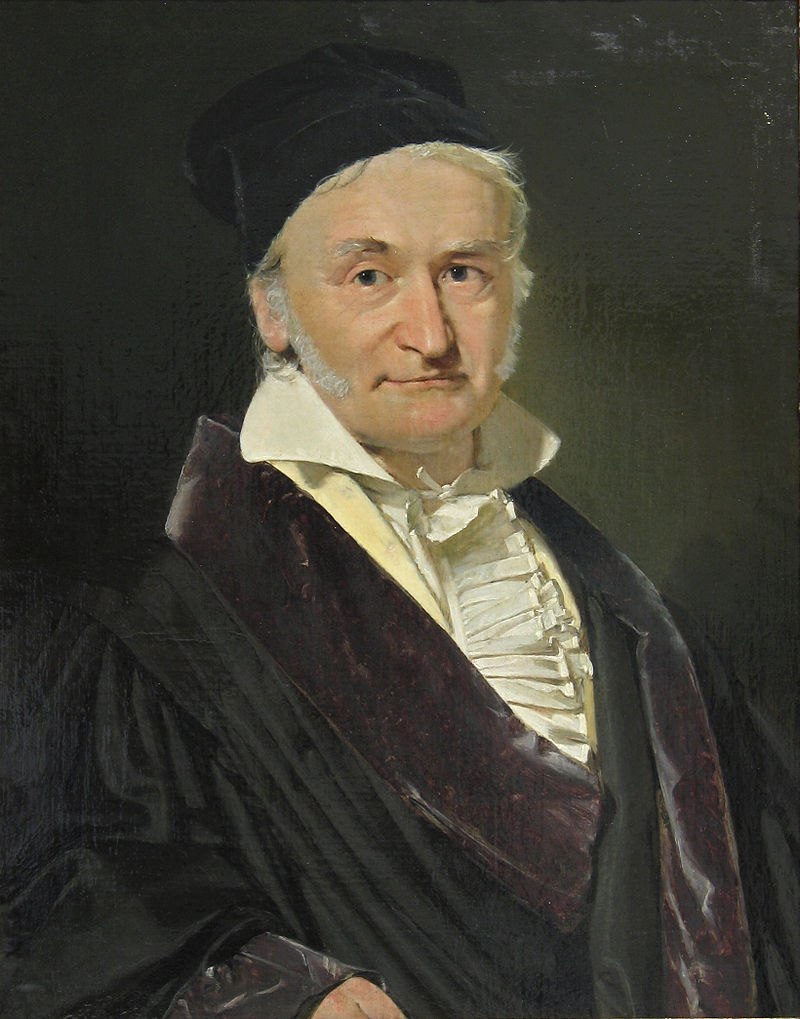
\includegraphics[width=0.4\textwidth]{imagenes/imagenes01/T01IM04.png}
	\end{figure}

Gauss fue un matemático, astrónomo, y físico alemán que contribuyó significativamente en muchos ámbitos, incluida la teoría de números, el análisis matemático, la geometría diferencial, la estadística, el álgebra, la geodesia, el magnetismo y la óptica. Considerado ya en vida como Princeps Mathematicorum, Gauss ha tenido una influencia notable en muchos campos de la matemática y de la ciencia.
\end{multicols}
Gauss pronto fue reconocido como un niño prodigio, pese a provenir de una familia campesina de padres con poca cultura: su madre sabía leer, aunque no escribir; su padre sí, pero en cuanto a las matemáticas, no pasaba de la aritmética más elemental. De Carl Friedrich Gauss existen muchas anécdotas acerca de su asombrosa precocidad. Hizo sus primeros grandes descubrimientos en el bachillerato, siendo a apenas un adolescente, y completó su magnum opus, Disquisitiones arithmeticae, a los veintiún años (1798), aunque se publicó en 1801. Fue un trabajo fundamental para consolidar la teoría de los números y ha moldeado esta área hasta los días presentes.

\end{myexampleblock}	
	

	
El método de Gauss para la solución de SEL es un método `muy robusto' y es aplicable a cualquier sistema independientemente de su número de ecuaciones o incógnitas. Es por ellos que se recomienda al lector/a que siga todos los ejercicios para asegurarse que entiende bien el método. En temas posteriores veremos otros métodos de resolución (Rouché, ecuaciones matriciales), que tendrán sus ventajas e inconvenientes respecto del método de Gauss pero no son tan potentes como éste.
 
Empezamos una colección de ejercicios resueltos en que se intentará que muestren explícitamente todos los pasos. El/la lector/a debe asegurarse que entiende bien todos los pasos y verse capaz de enfrentarse a los problemas propuestos con solución. Recuerda que cada problema es un mundo y solo al hacer muchos de ellos verás un abanico grande de posibilidades.

Los problemas de discusión de sistemas se dejan, como se ha mencionado anteriormente, para cuando se estudie el `teorema de Rocuché-Frobenius' que es una herramienta matemática más adecuada para estos menesteres.

También se incluyen, a modo de anécdota, algunos problemas de enunciado de los que hay que extraer el SEL correspondiente, resolver e interpretar la solución obtenida.
\subsection{Ejercicios resueltos}

Veamos un problema donde hay que intercambiar ecuaciones e incógnitas (avisando en este caso) para conseguir pivote $\pm 1$. Esto no es necesario, pero es conveniente para minimizar errores.

\begin{ejre} Resuelve: $\quad \begin{cases}2x+3y-4z=7\\3x+5y-z=6\\-3x+2y+5z=-3\end{cases}$ 
\end{ejre}
\begin{proofw}\renewcommand{\qedsymbol}{$\diamond$}
Matricialmente: $\quad \left[ \begin{matrix}
  2 & 3 & -4 \\ 3 & 5 & \boldsymbol{-1} \\ -3 & 2 & 5 
 \end{matrix}\right. 
 \left| \begin{matrix}
  7 \\ 6 \\ -3 
 \end{matrix}\right] \to$ 
\textcolor{gris}{$[E2 \leftrightarrow E1 ] \to (*)$}

Intercambiamos la ecuación 2 por la 1 y, luego, cambiamos de orden las incógnitas (*), para que el coeficiente $\boldsymbol{-1}$ aparezca en el lugar $1,1$ de la matriz y sea más sencillo combinar las otras ecuaciones con la primera para obtener ceros por debajo del $\boldsymbol{-1}$. Aunque no es necesario advertir del cambio de orden de las ecuaciones, sí lo es para el cambio de las incógnitas (lo hemos hecho añadiendo una fila a la matriz) ya que, de otro modo, pensaríamos que las incógnitas van en el orden habitual $x,y,z$.

$\left[ \begin{matrix}
  3 & 5 & \boldsymbol{-1} \\ 2 & 3 & -4 \\ -3 & 2 & 5 
 \end{matrix}\right. 
 \left| \begin{matrix}
  6 \\ 7 \\ -3  
 \end{matrix}\right] \to$
 $\left[ \begin{matrix}
  \boldsymbol{z} &  \boldsymbol{x} &  \boldsymbol{y} \\
  \boldsymbol{-1} & 3 & 5 \\ -4 & 2 & 3 \\ 5 & -3 & 2 
 \end{matrix}\right. 
 \left| \begin{matrix}
  \\ 6 \\ 7 \\ -3 
 \end{matrix}\right] \to$
 \textcolor{gris}{$\left[ \begin{matrix} E2 \to E2-4E1 \\ E3 \to E3+5E1 \end{matrix} \right] \to $}
 
 $\left[ \begin{matrix}
  z & x & y \\
 -1 & 3 & 5 \\ 0 & -10 & -17 \\ 0 & 12 & 27 
 \end{matrix}\right. 
 \left| \begin{matrix}
  \\ 6 \\ -17 \\ 27 
 \end{matrix}\right] \to$
 \textcolor{gris}{$[E3 \to 10E3-17E2] \to $}
 
  $\left[ \begin{matrix}
  z & x & \boldsymbol{y} \\
 -1 & 3 & 5 \\ 0 & -10 & -17 \\ 0 & 0 & 66 
 \end{matrix}\right. 
 \left| \begin{matrix}
  \\ 6 \\ -17 \\ 66 
 \end{matrix}\right] \to \begin{cases}
 \; \; 66y=66 \to \boldsymbol{y=1} \\
 \; -10x-17\cdot 1=-17 \to \boldsymbol{x=0}\\
 \; -z+3\cdot 0 + 5 \cdot 1 = 6 \to \boldsymbol{z=-1}	
 \end{cases}
$

Los transformaciones de Gauss escogidas para conseguir ceros no es necesario explicitarlas pero, de momento, lo haremos para dar más claridad al proceso.

!`Atención!: la última incógnita ahora es `$y$' no `$z$' como hemos indicado en la primera fila de la matriz. 

Despejando en cascada hemos encontrado	$\boldsymbol{x=0; \; y=1; \; z=-1}$, solución única: \textbf{SDC}.	
\end{proofw}

El método de Gauss no solo se aplica a `sistemas cuadrados', del mismo número de ecuaciones que de incógnitas si no que se puede aplicar en cualquier caso, con más ecuaciones que incógnitas o con más incógnitas que ecuaciones. En ambos casos el objetivo es el mismo, triangularizar la matriz, que por debajo de la diagonal todos los elementos sean ceros. Analizamos esto en los  siguientes ejercicios resueltos.
\begin{ejre} 
Resuelve: $\quad \left\{ \begin{matrix}
x&+2y&-5z&-t&+2u&=-3\\
&y&-2z&+t&-4u&=1\\
2x&-3y&+4z&+2t&-u&=9	
\end{matrix} \right.$
	
\end{ejre}
\begin{proofw}\renewcommand{\qedsymbol}{$\diamond$}

$\left[ \begin{matrix}
  1 & 2 & -5 & -1 & 2 \\ 0 & 1 & -2 & 1 & -4 \\ 2 & -3 & 4 & 2 & -1  
 \end{matrix}\right. 
 \left| \begin{matrix}
  -3 \\ 1 \\ 9 
 \end{matrix}\right] \to  $
$\left[ \begin{matrix}
  1 & 2 & -5 & -1 & 2 \\ 0 & 1 & -2 & 1 & -4 \\ 0 & -7 & 14 & 4 & -5  
 \end{matrix}\right. 
 \left| \begin{matrix}
  -3 \\ 1 \\ 15 
 \end{matrix}\right] \to  $
 
 \noindent \footnotesize{$\left[ \begin{matrix}
  1 & 2 & -5 & -1 & 2 \\ 0 & 1 & -2 & 1 & -4 \\ 0 & 0 & 0 & 11 & -33  
 \end{matrix}\right. 
 \left| \begin{matrix}
  -3 \\ 1 \\ 22 
 \end{matrix}\right] \to$}
 \scriptsize{$  \begin{cases}
  11t-33u=22; \; t-3u=2; u=\lambda \Rightarrow t=2+3\lambda \\
  y-2z+2+3\lambda-4\lambda=1; z=\mu \Rightarrow y=2\mu +\lambda -1\\
  x+2(2\mu+\lambda-1)-5\mu-2-3\lambda+2	\lambda=-3 \Rightarrow \\ \qquad  \qquad \qquad x=\mu-\lambda+1 \end{cases}$}\normalsize{.}



\noindent \small{$\boldsymbol {u=\lambda; \; t=2+3\lambda;\; z=\mu; \; y=2\mu+\lambda-1; \; x=\mu-\lambda+1\; \; \forall\; \lambda\; \mu \; \in \mathbb R }$}

Esta vez tenemos un \textbf{SCI}, doblemente indeterminado (hemos necesitado dos parámetros).
\end{proofw}


\begin{ejre} 
	Resuelve: $\quad \begin{cases}x+2y-3z=0\\-2x-z=-3\\-x+y=0\\-2y+4z=4\end{cases}$
\end{ejre}
\begin{proofw}\renewcommand{\qedsymbol}{$\diamond$}

$\left[ \begin{matrix}
  1 & 2 & -3 \\ -2 & 0 & -1 \\ -1 & 1 & 0 \\ 0 & -2 & 4  
 \end{matrix}\right. 
 \left| \begin{matrix}
  0 \\ -3 \\ 0 \\ 4
 \end{matrix}\right] \to $ 
 \textcolor{gris}{$\left[ \begin{matrix} E2 \to E2+2E1 \\ E3 \to E3+E1 \\ E4 \to E4\end{matrix} \right] \to $}
 $\left[ \begin{matrix}
  1 & 2 & -3 \\ 0 & 4 & -7 \\ 0 & 3 & -3 \\ 0 & -2 & 4  
 \end{matrix}\right. 
 \left| \begin{matrix}
  0 \\ -3 \\ 0 \\ 4
 \end{matrix}\right] \to $ 
 
 \noindent  \textcolor{gris}{$ \text{astucia:}\;  [E2 \leftrightarrow E3 ] \; \to $}
  $\left[ \begin{matrix}
  1 & 2 & -3 \\ 0 & 3 & -3 \\ 0 & 4 & -7 \\ 0 & -2 & 4  
 \end{matrix}\right. 
 \left| \begin{matrix}
  0 \\ 0 \\ -3 \\ 4
 \end{matrix}\right] \to $ \textcolor{gris}{$  \text{astucia:} \; [E2 \to E2/3]\; \to $}
 
 \noindent  $\left[ \begin{matrix}
  1 & 2 & -3 \\ 0 & 1 & -1 \\ 0 & 4 & -7 \\ 0 & -2 & 4  
 \end{matrix}\right. 
 \left| \begin{matrix}
  0 \\ 0 \\ -3 \\ 4
 \end{matrix}\right] \to $ \textcolor{gris}{$\left[ \begin{matrix}  E3 \to E3-4E2 \\ E4 \to E4+2E2 \end{matrix} \right] \to $}
 $\left[ \begin{matrix}
  1 & 2 & -3 \\ 0 & 1 & -1 \\ 0 & 0 & -3 \\ 0 & 0 & 42  
 \end{matrix}\right. 
 \left| \begin{matrix}
  0 \\ 0 \\ -3 \\ 4
 \end{matrix}\right] \to $ 
  
 \noindent \textcolor{gris}{$  \text{astucia:} \; [E3 \to E3/3]\; \to $}  $\left[ \begin{matrix}
  1 & 2 & -3 \\ 0 & 1 & -1 \\ 0 & 0 & -1 \\ 0 & 0 & 42  
 \end{matrix}\right. 
 \left| \begin{matrix}
  0 \\ 0 \\ -1 \\ 4
 \end{matrix}\right] \to $ \textcolor{gris}{$[E4 \to E4+42E3] \to $}
 
 \noindent  $\left[ \begin{matrix}
  1 & 2 & -3 \\ 0 & 1 & -1 \\ 0 & 0 & -1 \\ 0 & 0 & 0  
 \end{matrix}\right. 
 \left| \begin{matrix}
  0 \\ 0 \\ -1 \\ -38
 \end{matrix}\right] \to \; $ Última ecuación: $0=-38 \to \; $\textbf{SI}, el sistema no tiene solución.
\end{proofw}


\begin{ejre} 
Resuelve: $\quad \begin{cases}x-2y=0\\3x-y=5\\x-y=1\\x+y=3\\2x-3y=1\end{cases}$	
\end{ejre}
\begin{proofw}\renewcommand{\qedsymbol}{$\diamond$}

$\left[ \begin{matrix}
  1 & -2   \\ 3 & -1  \\ 1 & -1  \\ 1 & 1 \\ 2 & -3  
 \end{matrix}\right. 
 \left| \begin{matrix}
   0 \\ 5 \\ 1 \\ 3 \\ 1  
 \end{matrix}\right] \to \; $
 \textcolor{gris}{$\left[ \begin{matrix} E2 \to E2-3E1 \\ E3 \to E3-E1 \\ E4 \to E4-E1 \\ E5 \to E5-2E1   \end{matrix} \right] \to $} 
$\left[ \begin{matrix}
  1 & -2   \\ 0 & 5  \\ 0 & 1  \\ 0 & 3 \\ 0 & 1  
 \end{matrix}\right. 
 \left| \begin{matrix}
   0 \\ 5 \\ 1 \\ 3 \\ 1  
 \end{matrix}\right] \to \; $
 \textcolor{gris}{$  \text{astucia:} \; [E3 \leftrightarrow E2 ]\; \to $} 
 
 \noindent $\left[ \begin{matrix}
  1 & -2   \\ 0 & 1  \\ 0 & 5  \\ 0 & 3 \\ 0 & 1  
 \end{matrix}\right. 
 \left| \begin{matrix}
   0 \\ 1 \\ 5 \\ 3 \\ 1  
 \end{matrix}\right] \to \; $
 \textcolor{gris}{$\left[ \begin{matrix} E3\to E3-5E2 \\ E4\to E4-3E2 \\ E5 \to E5-E2  \end{matrix} \right] \to $}
 $\left[ \begin{matrix}
  1 & -2   \\ 0 & 1  \\ \text{\textst{ 0 }}  & \text{\textst{ 0 }}   \\ \text{\textst{ 0 }}  & \text{\textst{ 0 }}  \\ \text{\textst{ 0 }}  & \text{\textst{ 0 }}   
 \end{matrix}\right. 
 \left| \begin{matrix}
   0 \\ 1 \\ \text{\textst{ 0 }}  \\ \text{\textst{ 0 }}  \\ \text{\textst{ 0 }}   
 \end{matrix}\right] \to \; $ 
 
 Última ecuación (eliminadas las trivialidades): $\; \boldsymbol{y=1} \Rightarrow x-2=0 \to \boldsymbol{x=2}$

Tenemos un \textbf{SCD} cuya solución única es $\boldsymbol{x=2; \; y=1}$, que muchos autores pueden representar como $(2,1)$.
\end{proofw}


\begin{ejre} 
Resuelve: $ \quad \begin{cases}-x+y-z=-2\\x-y+2z=4\\x+z+t=3\\x+2z+t=1 \end{cases}$
\end{ejre}
\begin{proofw}\renewcommand{\qedsymbol}{$\diamond$}

$\left[ \begin{matrix}
 -1 & 1 & -1 & 0\\ 1 & -1 & 2 & 0 \\ 1 & 0 & 1 & 1 \\ 1 & 0 & 2 & 1 
 \end{matrix}\right. 
 \left| \begin{matrix}
  -2 \\ 4 \\ 3  \\ 1
 \end{matrix}\right] \to$
\textcolor{gris}{$\begin{cases} E2 \to E2+E1 \\ E3 \to E3+E1 \\ E4 \to E4+E1 \end{cases} \to $}
$\left[ \begin{matrix}
 1 & 1 & -1 & 0\\ 0 & 0 & 1 & 0 \\ 0 & 1 & 0 & 1 \\ 0 & 1 & 1 & 1 
 \end{matrix}\right. 
 \left| \begin{matrix}
  -2 \\ 2 \\ 1  \\ -1
 \end{matrix}\right] \to$
 
Intercambiamos las ecuaciones 2 y 3: \textcolor{gris}{$[\;E2 \leftrightarrow E3 \; ]$}

\noindent $\left[ \begin{matrix}
 1 & 1 & -1 & 0\\ 0 & 1 & 0 & 1 \\ 0 & 0 & 1 & 0 \\ 0 & 1 & 1 & 1 
 \end{matrix}\right. 
 \left| \begin{matrix}
  -2 \\ 1 \\ 2  \\ -1
 \end{matrix}\right] \to$ \textcolor{gris}{$\begin{cases} E3 \to E3 \\ E4 \to E4-E2 \end{cases} \to $}
 $\left[ \begin{matrix}
 1 & 1 & -1 & 0\\ 0 & 1 & 0 & 1 \\ 0 & 0 & 1 & 0 \\ 0 & 0 & 1 & 0 
 \end{matrix}\right. 
 \left| \begin{matrix}
  -2 \\ 1 \\ 2  \\ -2
 \end{matrix}\right] \to$
 


\noindent  \textcolor{gris}{$[\;E4 \to E4-E3 \;] \to $} $\left[ \begin{matrix}
 1 & 1 & -1 & 0\\ 0 & 1 & 0 & 1 \\ 0 & 0 & 1 & 0 \\ 0 & 0 & 0 & 0 
 \end{matrix}\right. 
 \left| \begin{matrix}
  -2 \\ 1 \\ 2  \\ -4
 \end{matrix}\right] \to$ Última ecuación: $0=-4$, hemos llegado a una incompatibilidad, tenemos pues un \textbf{SI}
\end{proofw}

\begin{ejre} 
Resuelve: $\; \begin{cases} 2x+3y+4z+5t=0\\-3x-2y+3z-2t=-2\\4x+5y-2z+2t=7  \end{cases}\; $  \footnotesize{\textcolor{gris}{sin ningún pivotes $\pm 1$}}\normalsize{.}
\end{ejre}
\begin{proofw}\renewcommand{\qedsymbol}{$\diamond$}

$\left[ \begin{matrix}
  2 & 3 & 4 & 5 \\ -3 & -2 & 3 & -2 \\ 4 & 5 & -2 & 2 
 \end{matrix}\right. 
 \left| \begin{matrix}
  9 \\ -2 \\ 7 
 \end{matrix}\right] \to $
 \textcolor{gris}{$\begin{cases} E2\to 2E2+3E1 \\ E3 \to E3-2E1  \end{cases} \to $}
$\left[ \begin{matrix}
  2 & 3 & 4 & 5 \\ 0 & 5 & 18 & 11 \\ 0 & -1 & -10 & -8 
 \end{matrix}\right. 
 \left| \begin{matrix}
  9 \\ 23 \\ -11 
 \end{matrix}\right] \to $
 
\noindent \textcolor{gris}{$[\; E3 \to 5E3+E2 \; ] \to $}
$\left[ \begin{matrix}
  2 & 3 & 4 & 5 \\ 0 & 5 & 18 & 11 \\ 0 & 0 & 32 & 29 
 \end{matrix}\right. 
 \left| \begin{matrix}
  9 \\ 23 \\ 32 
 \end{matrix}\right] \to 32z+29t=32; \; \boldsymbol{t=\lambda, \; \forall \lambda \in \mathbb R}$
 
 \noindent $\boldsymbol{z=1-\frac{29}{32}\lambda}; \; \to 5y+18(1-\frac{29}{32}\lambda)+11 \lambda =23 \to \boldsymbol{y=1-\frac {371}{80}\lambda}\; \to 2x+3(1-\frac {371}{80}\lambda)+4(1-\frac{29}{32}\lambda)+5\lambda = 9 \to \boldsymbol{x=1-\frac{1003}{160}\lambda}\; $. \textbf{SCI}.
\end{proofw}

\begin{ejre} 
Resuelve: $\quad \begin{cases} 5x-3y+4z=0\\2x+5y-z=0\\-3x-2y+6z=0   \end{cases}$ 
\end{ejre}
\begin{proofw}\renewcommand{\qedsymbol}{$\diamond$}
\small{$\left[ \begin{matrix}
  5 & -3 & 4 \\ 2 & 5 & -1 \\ -3 & -2 & 6 
 \end{matrix}\right. 
 \left| \begin{matrix}
  0 \\ 0 \\ 0 
 \end{matrix}\right] \to $}
\small{\textcolor{gris}{$E2\leftrightarrow E1 \to $}}
 $\left[ \begin{matrix}
   2 & 5 & -1  \\ 5 & -3 & 4 \\ -3 & -2 & 6 
 \end{matrix}\right. 
 \left| \begin{matrix}
  0 \\ 0 \\ 0 
 \end{matrix}\right]  \to $
 \footnotesize{\textcolor{gris}{Intercambio $x\leftrightarrow z \to$}}
 
\normalsize{ \noindent  $\left[ \begin{matrix}
  \boldsymbol{z} & \boldsymbol{y} & \boldsymbol{x} \\
   -1 & 5 & 2  \\ 4 & -3 & 5 \\ 6 & -2 & -3 
 \end{matrix}\right. 
 \left| \begin{matrix}
 \\ 0 \\ 0 \\ 0 
 \end{matrix}\right]  \to $
 \textcolor{gris}{$\begin{cases} E2\to E2+4E1 \\ E3 \to E3+6E1 \end{cases} \to $}
  $\left[ \begin{matrix}
  \boldsymbol{z} & \boldsymbol{y} & \boldsymbol{x} \\
   -1 & 5 & 2  \\ 0 & 17 & 13 \\ 0 & 28 & 11 
 \end{matrix}\right. 
 \left| \begin{matrix}
 \\ 0 \\ 0 \\ 0 
 \end{matrix}\right]  \to $}
 
 \noindent \textcolor{gris}{$[E3 \to 17E3-28E2]\to $}
   $\left[ \begin{matrix}
  \boldsymbol{z} & \boldsymbol{y} & \boldsymbol{x} \\
   -1 & 5 & 2  \\ 0 & 17 & 13 \\ 0 & 0 & -183 
 \end{matrix}\right. 
 \left| \begin{matrix}
 \\ 0 \\ 0 \\ 0 
 \end{matrix}\right]  \to -183x=0 \Rightarrow \boldsymbol{x=y=z=0}\; $ \normalsize{SCD y homogéneo, solo tiene la solución trivial.}

\end{proofw}

\begin{ejre} 
Resuelve: $\quad \begin{cases} x+2y-3z=0\\2x+y-z=0\\x-y+2z=0  \end{cases}$ 
\end{ejre}
\begin{proofw}\renewcommand{\qedsymbol}{$\diamond$}
$\left[ \begin{matrix}
  1 & 2 & -3 \\ 2 & 1 & -1 \\ 1 & -1 & 2 
 \end{matrix}\right. 
 \left| \begin{matrix}
  0 \\ 0 \\ 0 
 \end{matrix}\right] \to $
 \textcolor{gris}{$\begin{cases} E2 \to E2-2E1 \\ E3 \to E3-E1  \end{cases} \to $}
 $\left[ \begin{matrix}
  1 & 2 & -3 \\ 0 & -3 & 5 \\ 0 & -3 & 5 
 \end{matrix}\right. 
 \left| \begin{matrix}
  0 \\ 0 \\ 0 
 \end{matrix}\right] \to $
 
 \noindent \textcolor{gris}{$[ E3 \to E3-E2] \to$}
  $\left[ \begin{matrix}
  1 & 2 & -3 \\ 0 & -3 & 5 \\ \text{\textst{ 0 }} 
 & \text{\textst{ 0 }} 
 & \text{\textst{ 0 }} 
 
 \end{matrix}\right. 
 \left| \begin{matrix}
  0 \\ 0 \\ \text{\textst{ 0 }} 
 \end{matrix}\right] \to $ Eliminando la trivialidad, la última ecuación dice: $-3y+5z=0 \to \boldsymbol{z=\lambda , \; \forall \lambda \in \mathbb R} ;\; \boldsymbol{y=\frac 5 3 \lambda}; \; \; x+2 \frac 5 3 \lambda -3\lambda =0 \to \bold{x=-\frac 1 3 \lambda} $. Tenemos un \textbf{SCI}, como es homogéneos debe contener a la solución trivial. Basta, para ello, tomar $\lambda=0$.
\end{proofw}

\begin{ejre} 
Resuelve: $\begin{cases} x+y+z+t&=0\\x-2y+3z&=0\\2x-y+4z+t&=0 \end{cases}$
\end{ejre}
\begin{proofw}\renewcommand{\qedsymbol}{$\diamond$}
$\left[ \begin{matrix}
  1 & 1 & 1 & 1 \\ 1 & -2 & 3 & 0\\ 2 & -1 & 4 & 1 
 \end{matrix}\right. 
 \left| \begin{matrix}
  0 \\ 0 \\ 0 
 \end{matrix}\right] \to$
 \textcolor{gris}{$\begin{cases} E2\to E2-E1\\E3\to E3-2E1 \end{cases} \to  $}
$\left[ \begin{matrix}
  1 & 1 & 1 & 1 \\ 0 & -3 & 2 & -1\\ 0 & -3 & 2 & -1 
 \end{matrix}\right. 
 \left| \begin{matrix}
  0 \\ 0 \\ 0 
 \end{matrix}\right] \to$
 	
\noindent \textcolor{gris}{$[E3 \to E3-E2] \to $}
$\left[ \begin{matrix}
  1 & 1 & 1 & 1 \\ 0 & -3 & 2 & -1\\ \text{\textst{ 0 }} & \text{\textst{ 0 }} & \text{\textst{ 0 }} & \text{\textst{ 0 }} 
 \end{matrix}\right. 
 \left| \begin{matrix}
  0 \\ 0 \\ \text{\textst{ 0 }} 
 \end{matrix}\right] \to$ última ecuación:
 
 \noindent $-3y+2z-t=0; \boldsymbol{y=\lambda ;\;  z=\mu; \; \forall \lambda, \mu \; \in \mathbb R}\to \boldsymbol{t=-3\lambda+2\mu} \to x+\lambda+\mu+(-3\lambda+2\mu)=0 \to \bold{x=2\lambda-3\mu}; \; SCI$

\end{proofw}


\begin{ejre} 
Como se comenta al principio de la sección ejercicios, el método de Gauss-Jordan es una ampliación del método de Gauss que consiste en, una vez triangularizada inferiormente la matriz asociada al SEL (ceros por debajo de la diagonal), hacerlo ahora por arriba. De este modo queda una matriz `diagonalizada' en la que de cada fila se despeja cada incógnita.

\noindent Resuelve, por el método de Gauss- Jordan el SEL : $\begin{cases}  x+2y-z&=-2 \\ x+z&=2 \\ 2x-y+2z&=5\end{cases}$
\end{ejre}
\begin{proofw}\renewcommand{\qedsymbol}{$\diamond$}

$\left[ \begin{matrix}
  1 & 2 & -1 \\ 1 & 0 & 1 \\ 2 & -1 & 2 
 \end{matrix}\right. 
 \left| \begin{matrix}
  -2 \\ 2 \\ 5  
 \end{matrix}\right] \to  $
 \textcolor{gris}{$\begin{cases}E2 \to E2-E1 \\ E3 \to E3-2 E1 \end{cases} $}
 $ \to \left[ \begin{matrix}
  1 & 2 & -1 \\ 0 & -2 & 2 \\ 0 & -5 & 4 
 \end{matrix}\right. 
 \left| \begin{matrix}
  -2 \\ 4 \\ 9  
 \end{matrix}\right] \to$
 
 \noindent \textcolor{gris}{$[E2 \leftrightarrow E2/2 ] $}
 $ \to \left[ \begin{matrix}
  1 & 2 & -1 \\ 0 & -1 & 1 \\ 0 & -5 & 4 
 \end{matrix}\right. 
 \left| \begin{matrix}
  -2 \\ 2 \\ 9  
 \end{matrix}\right] \to$
  \noindent \textcolor{gris}{$[E3 \leftrightarrow E3-5E1 ] $}
  $ \to \left[ \begin{matrix}
  1 & \boxed{2} & \boxed{-1} \\ 0 & -1 & \boxed{1} \\ 0 & 0 & -1 
 \end{matrix}\right. 
 \left| \begin{matrix}
  -2 \\ 2 \\ -1  
 \end{matrix}\right] \to$
  \textcolor{gris}{Ahora, al revés: $\begin{cases}E2 \to E2+E3 \\ E1 \to E1-E3 \end{cases} $}
   $ \to \left[ \begin{matrix}
  -1 & \boxed{-2} & 0 \\ 0 & -1 & 0 \\ 0 & 0 & -1 
 \end{matrix}\right. 
 \left| \begin{matrix}
  1 \\ 1 \\ -1  
 \end{matrix}\right] \to$
 \textcolor{gris}{$\left[\begin{matrix}E3\to \\ E3-E2\end{matrix} \right]$}
 
 \noindent    $ \to \left[ \begin{matrix}
  -1 & 0 & 0 \\ 0 & -1 & 0 \\ 0 & 0 & -1 
 \end{matrix}\right. 
 \left| \begin{matrix}
  -1 \\ 1 \\ -1  
 \end{matrix}\right] \to \begin{matrix} \text{ matriz } \\ \text{diagonalizada}  \end{matrix} \to \begin{cases} \; -x=-1 \to \boldsymbol{x=1} \\ \; -y=1 \to \boldsymbol{y=-1} \\ \; -z=-1 \to \boldsymbol{z=1}   \end{cases}\; \; \boldsymbol{SCD}$
\end{proofw}

\begin{ejre} 
Encuentra una solución, si es posible, del siguiente sistema en que $z=3$. ?`Existe alguna solución en que $x=2$?

$\begin{cases} x-y+z=1\\x+y-z=1\\5x+y-z=5  \end{cases}$
\end{ejre}
\begin{proofw}\renewcommand{\qedsymbol}{$\diamond$}
Apliquemos el método de Gauss para resolver el sistema y encontrar todas sus soluciones y luego ya intentaremos contestar a las preguntas que nos formulan.

$\left[ \begin{matrix}
  1 & -1 & 1 \\ 1 & 1 & -1 \\ 5 & 1 & -1 
 \end{matrix}\right. 
 \left| \begin{matrix}
  1 \\ 1 \\ 5 
 \end{matrix}\right] \to $
 $\left[ \begin{matrix}
  1 & -1 & 1 \\ 0 & 2 & -2 \\ 0 & 6 & -6 
 \end{matrix}\right. 
 \left| \begin{matrix}
  1 \\ 0 \\ 0 
 \end{matrix}\right] \to $
  $\left[ \begin{matrix}
  1 & -1 & 1 \\ 0 & 2 & -2 \\ \text{\textst{ 0 }} & \text{\textst{ 0 }} & \text{\textst{ 0 }} 
 \end{matrix}\right. 
 \left| \begin{matrix}
  1 \\ 0 \\ \text{\textst{ 0 }}
 \end{matrix}\right] \to $
 
 $2y-2z=0; \; \boldsymbol{z=\lambda}, \; ºforall \lambda \in \mathbb R \to -\lambda+\lambda=1 \to \boldsymbol{x=1}$
 
 Tenemos un $\textbf{SCI}, \text{ con soluciones : } x=1; \; y=\lambda; \; z=\lambda; \quad \forall \lambda \in \mathbb R$. Respondamos ahora a las preguntas del problema:
 
--- Encuentra una solución, si es posible, del siguiente sistema en que $z=3 \Rightarrow $ \textbf{Sí}, ya que si $z=3=\lambda \to y=3; \; x=1$
 
 --- ?`Existe alguna solución en que $x=2$? \textbf{No}, necesariamente, en todas las soluciones $x=1$
 
\end{proofw}

\begin{ejre} 
En ocasiones, ante la sencillez del problema, no es necesario seguir todos los pasos.

Resuelve: 

$a) \quad \begin{cases} 2x-3z&=2\\2x+3y-4z&=-1\\z&=0 \end{cases} \qquad \qquad b) \quad \begin{cases} y+z&=4\\x-3y+2z&=7\\y-z&=2 \end{cases}$
\end{ejre}
\begin{proofw}\renewcommand{\qedsymbol}{$\diamond$}
a) En este caso, usando un poco la astucia no hace falta hacer nada (colocamos $z$ como primera incógnita, luego $x$ e $y$ por último. Escribimos como primera ecuación la tercera, como segunda la primera y como tercera la segunda y ya tenemos el sistema escalonado). 

Última ecuación $\boldsymbol{z=0}$, yendo a la primera ecuación: $2x-3\cdot0=2 \to \boldsymbol{x=1}$ y, finalmente, acudiendo a la segunda ecuación: $2\cdot 1 +3y-4\cdot 0=-1 \to \boldsymbol{y=-1}$, Tenemos un \textbf{SDC}.

b) Las ecuaciones uno y tres se resuelven inmediatamente sin más que sumarlas, $2y=6 \to \boldsymbol{y=3}$; sustituyendo en la primera, $3+z=4 \to \boldsymbol{z=1}$ y, finalmente, acudiendo a la segunda ecuación: $x-3\cdot 3 +2\cdot 2=7 \to \boldsymbol{x=14}$. Se trata de un \textbf{SCD}.
\end{proofw}


\begin{ejre} 
Un automóvil sube las cuestas a $54\; km/h$, las baja a $90\; km/h$ y en llano circula a $80\;  km/h$. Para ir de $A$ a $B$ tarda $2$ horas y 30 minutos, y para volver de $B$ a $A$, 2 horas y 45 minutos. ¿Cuál es la longitud de camino llano entre $A$ y $B$ si sabemos que la distancia entre $A$ y $B$ es de $192\;  km$? 
\end{ejre}
\begin{proofw}\renewcommand{\qedsymbol}{$\diamond$}
\begin{figure}[H]
		\centering
		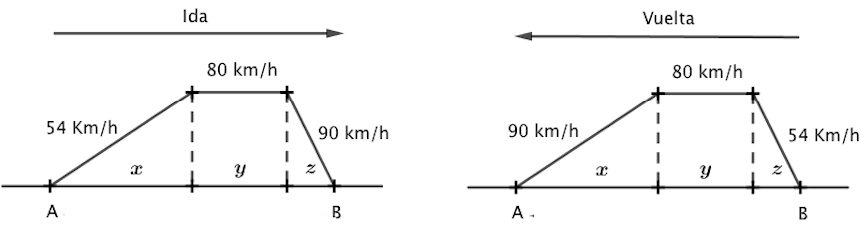
\includegraphics[width=.9\textwidth]{imagenes/imagenes01/T01IM06.png}
	\end{figure}

\vspace{-2mm}	

	Suponiendo que el vehículo viaja a $v$ constante: $v=\frac s t \to t=\frac s v$. A la ida $t_{ida}=t_{x,s}+t_{y,n}+t_{z,b}$, a la vuelta $t_{vuelta}=t_{x,b}+t_{y,n}+t_{z,s}$, donde los subíndices $\; x,y,z\; $ indican los tramos que circula el coche a distintas velocidades y $\; s,n,b\; $ indican los tramos de `subida', `normal' y `bajada', respectivamente.
	
	La traducción del enunciado al leguaje algebraico conduce al sistema:
	
	$\begin{cases} x+y+z&=192\\ \frac{x}{54} + \frac{y}{80}+\frac{z}{90}&=2.5 \\ \frac{x}{90}+\frac{y}{80}+\frac{z}{94}&=2.75   \end{cases} \; \; $
	Lo más cómodo es multiplicar las ecuaciones 2 y 3 por el mcm de los denominadores (2160, en este caso) y conseguir un sistema sin denominadores que, resolviendo por Gauss tiene por solución única (\textbf{SCD}):
	
	$\boldsymbol{x=31.725 \; km; \; y= 94.800 \; km; \; z= 65.465 \; km}$, con lo que \textbf{la longitud de camino llano es de} $\boldsymbol{94.8 \; km}$.
\end{proofw}


\begin{ejre} 
Un cajero automático contiene $95$ billetes de $10$, $20$ y $m$ euros. Se sabe que tiene almacenados $2000$ euros y que el número de billetes de $10$ euros es el doble que el número de billetes de $20$ euros. 

\begin{enumerate}[a) ]
\item Plantea un sistema de ecuaciones que refleje las condiciones del problema. ?`Qué valores puede tomar $m$?
\item Resuelve el sistema para $m=5$ y para  $m = 50$. 
\end{enumerate} 
\end{ejre}
\begin{proofw}\renewcommand{\qedsymbol}{$\diamond$}
Planteemos y resolvamos el problema y, después, contestaremos a las preguntas que se formulan.

Llamamos $x$ al número de billetes de $10$ euros, $y$ al número de billetes de $20$ euros y $z$ al número de billetes de $m$ euros. Con esto, el sistema es:

\noindent $\begin{cases}x+y+z=95\\10x+20y+mz=2000\\x=2y  \end{cases}$. Sistema que hay que preparar antes de aplicar el método de Gauus pasando todas las incógnitas a la izquierda y los términos independientes a la derecha. Aprovechamos para escribir la segunda ecuación en último lugar y usar el parámetro $m$ lo más tarde posible. Ya advertimos que para discutir sistemas veremos métodos mejores que Gauss, pero en este caso vamos a resolverlo.

\noindent $\begin{cases}x+y+z=95 \\x-2y=0 \\10x+20y+mz=2000  \end{cases} \to $
$\left[ \begin{matrix}
  1 & 1 & 1 \\ 1 & -2 & 0 \\ 10 & 20 & m 
 \end{matrix}\right. 
 \left| \begin{matrix}
  95 \\ 0 \\ 2000 
 \end{matrix}\right] \to $
\textcolor{gris}{ $ \begin{cases} E2 \to E2-E1 \\ E3 \to E3-10E1 \end{cases} \to $}

\noindent $\left[ \begin{matrix}
  1 & 1 & 1 \\ 0 & -3 & -1 \\ 0 & 10 & m-10 
 \end{matrix}\right. 
 \left| \begin{matrix}
  95 \\ -95 \\ 1050 
 \end{matrix}\right] \to $
 \textcolor{gris}{$[E3 \to 3E3+10E2] \to $}
  $\left[ \begin{matrix}
  1 & 1 & 1 \\ 0 & -3 & -1 \\ 0 & 0 & 3m-40 
 \end{matrix}\right. 
 \left| \begin{matrix}
  95 \\ -95 \\ 2200
 \end{matrix}\right]  $
 
 Última ecuación: $(3m-40)z=2200$, el sistema es incompatible si $3m-40=0\to m=40/3 \notin \mathbb N$, como $m$ hace referencia a billetes de determinada cantidad, $m \in \{5,10,20,100, 200, 500\}$, luego es sistema es siempre \textbf{SCD} para los posibles valores de $m$.
 
 Aunque el enunciado pide analizar los casos $m=5$ y $m=50$, vamos a estudiar todas las posibilidades:
 
\noindent  --- $m=5 \to (3m-40)z=(15-40)z=2200\to z<0$, no tiene sentido una cantidad de billetes negativa.  No hay solución.
 
\noindent  --- $m=10 \to (3m-40)z=(10-40)z=-10z=2200\to z<0$, no tiene sentido una cantidad de billetes negativa.  No hay solución.
 
  
\noindent  --- $m=50 \to (3m-40)z=(150-40)z=110z=2200\to z=20; \; 3y+20=95\to y=25; \; x+25+20=95 \to x=50$, la solución es \textbf{50 billetes de 1o euros, 25 de 20 euros y 20 de 50 euros.}
 
\noindent  --- $m=100 \to (3m-40)z=(300-40)z=260z=2200 \to z=8.46\cdots \notin \mathbb N$. No hay solución.
 
 \noindent  --- $m=200 \to (3m-40)z=(600-40)z=560z=2200 \to z=3.92\cdots \notin \mathbb N$. No hay solución.
  
\noindent  --- $m=500 \to (3m-40)z=(1500-40)z=1460z=2200 \to z=1.50\cdots \notin \mathbb N$. No hay solución.
\end{proofw}

\begin{ejre}
	Razona si los siguientes sistemas son equivalentes o no: $\quad \begin{cases}x-3y+4z&=7\\3x+2z&=0 \end{cases} \qquad \qquad \qquad  \begin{cases}x=-2\\y=1\\z=3 \end{cases}$
	
	\noindent ?`Puedes añadir una ecuación al primer sistema para que resulte incompatible?
\end{ejre}
\begin{proofw}\renewcommand{\qedsymbol}{$\diamond$}
	El segundo sistema es SCD, su única solución es $(-2,1,3)$, que también es solución del primer sistema. Pero éste tiene infinitas soluciones puesto que se trata de un sistema con más incógnitas que ecuaciones que admite, al menos, una solución (no es SI). El primer sistema es pues SCI, por lo que los dos sistemas \textbf{no son equivalentes}.
	
	Para añadir una ecuación más al primer sistema y que resulte incompatible la ecuación añadida debe ser de la forma: $a(x-3y+4z)+b(3x+2z)\neq a\cdot 7+b \cdot 0$, Por ejemplo, con $a=b=1$, si se añade la ecuación $(x-3y+4z)+(3x+2z)=1 \rightarrow \boldsymbol{4x-3y+6z=1}$, tendremos un SI
\end{proofw}

\begin{ejre}
Considera el SEL: $\begin{cases} 2x-y+z=5 \\ -x+2y=3  \end{cases}$.

Añade, si es posible, una nueva ecuación al sistema para que resulte:  a) Incompatible, b) Compatible indeterminado, c) Compatible determinado. Justifica tus respuestas.
\end{ejre}
\begin{proofw}\renewcommand{\qedsymbol}{$\diamond$}
	Añadir una ecuación para que se produzca incompatibilidad consiste en añadir una contradicción, por ejemplo, si la primera ecuación da 5 y la segunda 3, la suma no puede ser nada que no sea 8. Por otra parte, añadir una ecuación para que el sistema sea compatible indeterminado consiste en añadir una trivialidad, algo que no aporte ninguna nueva información al sistema, por ejemplo, ecuación1 + ecuación 2 = 5+3=0. El sistema será compatible si hay solución única. Por ejemplo, dando un valor a $x$, de la segunda ecuación obtenemos la $y$ y despejamos en la primera. Sería suficiente con añadir una tercera ecuación de la forma $x=k$.
	
	--- SI: $a(2x-y+z)+b(-x+2y)\neq 5a+3b \to (a=b=1) \Rightarrow \boldsymbol{x+y+z=5}$
	
	--- SCI:  $a(2x-y+z)+b(-x+2y)= 5a+3b \to (a=b=1) \Rightarrow \boldsymbol{x+y+z=8}$
	
	---SCD: $\boldsymbol{x=1}$
\end{proofw}

\begin{ejre}
	Pon un ejemplo, cuando sea posible de un sistema de dos ecuaciones con tres incógnitas que sea: a) compatible determinado; b) compatible indeterminado; c) incompatible.
\end{ejre}
\begin{proofw}\renewcommand{\qedsymbol}{$\diamond$}
	
	\noindent a) Un sistema con menos ecuaciones que incógnitas jamás puede ser compatible determinado, con solo dos datos no podemos determinar tres valores (incógnitas).
	
	\noindent b) Un ejemplo sencillo es el siguiente sistema: $\begin{cases} x=1 \\y+z=1 \end{cases}$, de soluciones $(1,-\lambda,\lambda)$
	
	\noindent c) Un sistema incompatible con dos ecuaciones es que entren en contradicción. por ejemplo: $\begin{cases}x+y+z=1\\x+y+z=0\end{cases}$
\end{proofw}


\subsection{Ejercicios propuestos}
	\begin{figure}[H]
		\centering
		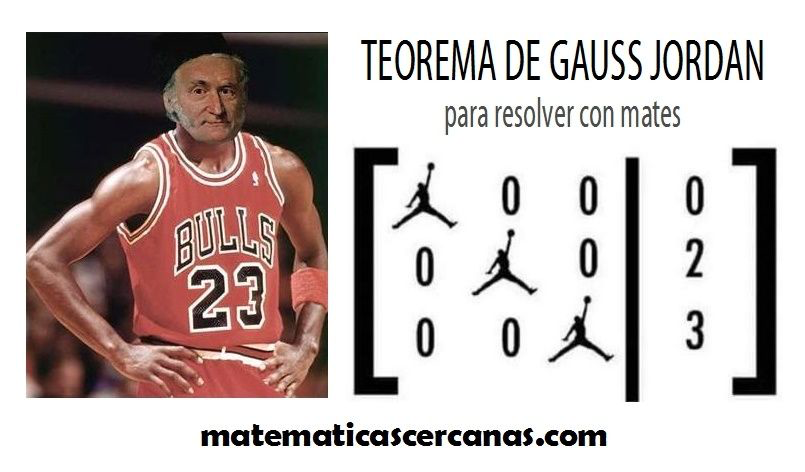
\includegraphics[width=0.8\textwidth]{imagenes/imagenes01/T01IM03.png}
	\end{figure}

\begin{enumerate}
\item $a) \quad \begin{cases}2x+6y+7z&=7\\x+2y-z&=-1\\5x+7y-4z&=9  \end{cases}\qquad b) \quad \begin{cases} x+y+z&=0\\x+2y+3z&=0\\3x+5y+7z&=1 \end{cases}$

\rightline{\textcolor{gris}{Solución: $a) \quad (10,-3,5); \; SCD; \qquad b) \quad SI$   }}

\item $a) \quad \begin{cases} 2x-y&=0\\-x+2y-z&=0\\-y+2z-t&=0\\-z+2t&=5 \end{cases} \qquad b) \quad \begin{cases} x+y-z&=2\\3x+3y+z&=2\\x+z=0\end{cases}$

\rightline{\textcolor{gris}{Solución: $a) \quad (1,2,3,4); \; SCD \qquad b) \quad (1,0,-1);\; SCD $ }}

\item $\qquad \begin{cases} x+y-3z-u&=-3\\x-y+2z-t&=-1\\4x-2y+6z+3t-4u&=3\\2x+4y-2z+4t-7u&=4 \end{cases}$

\rightline{\textcolor{gris}{Solución: $\left(\frac{7\lambda-2\mu-7}{2},\frac{5\lambda+2\mu-5}{2},\mu,3\lambda-3,\lambda \right)$  }}

\item $a) \quad \begin{cases} 3x-2y&=5\\x+4y&=4\\-x-2y&=-3  \end{cases}\qquad b) \quad \begin{cases} x+2z&=3\\x+y=2 \end{cases}$

\rightline{\textcolor{gris}{Solución: $a)\quad (2,1/2); \; SCD \qquad b) \quad (\lambda, 2-\lambda, (3-\lambda)/2); \; SCI$  }}

\item $a) \quad \begin{cases} -x+3y-z&=4\\x+4y&=5\\2x-6y+2z&=3  \end{cases}  \qquad b) \quad \begin{cases} 2x-y+z&=3\\x+2y-z&=4\\x-8y+5z&=-6 \end{cases}$

\rightline{\textcolor{gris}{Solución: $a)\quad SI; \qquad b) \quad (2-\lambda/5, 1+3\lambda/5,\lambda); \; SCI$  }}

\item $a) \quad \begin{cases} 3x-z&=4\\y+3x&=2 \end{cases} \qquad b) \quad \begin{cases} x+y+z&=1\\2x-3z&=5\\2y+5z&=2 \end{cases}$

\rightline{\textcolor{gris}{Solución: $a) \quad \left (\frac {4+\lambda} {3},2-3\lambda, \lambda \right) ; \; SCI \qquad b) \quad SI$  }}

\item $a) \quad \begin{cases} -3x+y+z&=1\\x-2y+z&=4\\-x+y-3z&=-7 \end{cases} \qquad b) \quad \begin{cases}2x-y+z&=3\\3x+y-z&=-3\\x-3y+3z&=9\\2x+4y-4z&=-12  \end{cases}$ 

\rightline{\textcolor{gris}{Solución: $a) \quad (0,1,-2); \; SCD \qquad b) \quad (2, \lambda -3, \lambda) \; \; SCI$ }}



\item $a) \quad \begin{cases}  x-y+z+t &= 0\\x+y+z-t &= 2\\x-y-z+t &= 2 \end{cases} \qquad b) \quad \begin{cases} 5x-y+3z &= -6\\x+3y-z &= 10\\2x-y+4z & =-2 \end{cases}$

\rightline{\textcolor{gris}{Solución: $a) \quad (2, 1+\lambda, -1, \lambda); \; SCI \qquad b) \quad (-1,4,1)$  }}

\item $a) \quad \begin{cases} 2x-y+z &= 5 \\ 3x+2y &= 1 \\ -x+4y-2z &= -9 \\ 6x+11y-3z &= -11  \end{cases} \qquad b) \quad \begin{cases} x+2y+z+t&=3\\-x+y+2t&=-1\\-x+7y+2z+8t&=1 \end{cases}$

\rightline{\textcolor{gris}{Solución: $a) \quad \left(\frac{11-2\lambda}{7}, \frac {-13+3\lambda}{7}, \lambda \right); \; SCI \qquad b) \quad SI$  }}

\item $a) \quad \begin{cases} 3x-5y+z&=0\\x-2y+z&=0\\x+y&=0 \end{cases} \qquad b) \quad \begin{cases} x-y-z&=0\\x+y+3z&=0\\x-5y-9z&=0 \end{cases}$

\rightline{\textcolor{gris}{Solución: $a) \quad (0,0,0)\; SCD \qquad b) \quad (-\lambda, -2\lambda, \lambda); \; SCI$  }}

\item $a) \quad \begin{cases} x+11y-4z&=0\\-2x+4y+z&=0\\ x+y-2z&=0\\2x-16y+5z&=0 \end{cases} \qquad b) \quad \begin{cases}   x+y+5z&=0\\3x-y-2t&=0\\x-y+z-t&=0\end{cases}$

\rightline{\textcolor{gris}{Solución: $a) \quad (0,0,0)\; SCD \qquad b) \quad (\lambda, -\lambda, 0, 2\lambda)\; \; SCI$  }}

\item $a) \quad \begin{cases} x-2y+3z&=0\\y+z&=0\\x-3y+2z&=0\\-x+5y&=0 \end{cases} \qquad b) \quad \begin{cases} x+3z&=0\\y-t&=0\\x+y+2t&=0\\2x+2y+3z+9t&=0 \end{cases}$

\rightline{\textcolor{gris}{Solución: $a) \quad (-5\lambda, -\lambda, \lambda); \; SCI \qquad b) \quad (0,0,0,0)\; \; SCD$  }}

\item Resuelve el sistema $\quad \begin{cases} -x+y&=1\\3x-y&=1  \end{cases}$

Añade una nueva ecuación al sistema, si es posible para que sea:

a) SCD; \hspace{10mm} b) SCI; \hspace{10mm} c) SI

\rightline{\textcolor{gris}{Solución: Solución sistema $(1,2);\;  a) x=1; \; b) No; \; c) x=3$   }}

\item ?`El siguiente sistema es compatible o incompatible? $\begin{cases} 3x-2y+4z&=6\\-2x+4y-z&=3\\x+2y+3z&=1  \end{cases}$

?`Se puede conseguir que sea SCI eliminando una ecuación?

\rightline\footnotesize{{\textcolor{gris}{Solución: $E3=E1+E2$, pero el término indep. debería ser $9$, no $1 \to SI. \quad$ Al eliminar una ecuación quedan 2 ecuaciones con 3 incógnitas, a los sumo puede ser SCI  }}}

\item Considera el sistema $\quad \begin{cases} 2x-2y-z&=4\\x+2y-2z&=1\\x-z&=1  \end{cases}$

a) ?`Existe una solución en que $y=0$?, encuéntrala si se da el caso.

b) Resuelve el sistema homogéneo asociado al dado.

\rightline{\textcolor{gris}{Solución: $a)\; (3,0,2),\; SCD \quad b)\; (2\lambda, \lambda, 2\lambda), \; SCI$  }}


\item Disponemos de tres lingotes de distintas aleaciones de tres metales A, B y C.  El primer lingote contiene 20 g del metal A, 20 g del B y 60 del C. El segundo contiene 10 g de A,  40 g de B y 50 g de C.  El tercero contiene 20 g de A,  40 g de B y 40 g de C.  Queremos elaborar, a partir de estos lingotes,  uno nuevo que contenga 15 g de A, 35 g de B y 50 g de C. ¿Cuántos gramos hay que coger de cada uno de los tres lingotes? 

\rightline{\textcolor{gris}{Solución: $25 \; g$ del primer lingote, $50\; g$ del segundo y $25\; g$ del tercero.  }}

\item Un estado compra 540 000 barriles de petróleo a tres suministradores diferentes que lo venden a 27,28 y 32 dólares el barril, respectivamente. La factura total asciende a 16 346 000 dólares. Si del primer suministrador recibe el 30 $\%$ del total de petróleo comprado, ¿cuál es la cantidad comprada a cada suministrador? 

\rightline{\textcolor{gris}{Solución: 162000 barriles al primero, 31000 al segundo y 347000 al tercero.  }}

\item De un número de tres cifras se sabe que la suma de estas es 13. Si se intercambian las cifras de las unidades y las centenas, el número disminuye en 198; y, si se intercambian las de la unidades y decenas, el número aumenta en 36. Encuentra el número. 

\rightline{\textcolor{gris}{Solución: $715$  }}

\item Si la altura de Luis aumentase el triple de la diferencia entre la altura de Eusebio y de Pablo,  Luis sería igual de alto que Pablo.  Las alturas de los tres suman 515 cm.  Ocho veces la altura de Eusebio es lo mismo que nueve veces la de Luis. Halla las tres alturas

\rightline{\textcolor{gris}{Solución: Luís $160\; cm$, Eusebio $180\; cm$ y Pablo $175 \; cm$  }}

\item  Tres jugadores acuerdan: ``Quien pierda una partida paga el doble del dinero que tengan los otros dos". Tras perder una partida cada uno, cada jugador tiene $200$ euros. ?`Con cuanto dinero empieza cada jugador?

\rightline{\textcolor{gris}{Solución: $363,\; 185,\; 52\;$ euros, por orden de pérdida de partida  }}

\item  Tres amigos juegan tres partidas de modo que cada vez que uno pierda entregará a ls otros una cantidad de dinero igual a que cada de ellos tenga en ese momento. Cada jugador pierde una partida y, al final, acaban con 24 euros cada uno de llos. ?`Con cuánto dinero empezaron?

\rightline{\textcolor{gris}{Solución: $39,\; 21,\; 12\;$ euros, por orden de pérdida de partida  }}

\item En una excavación arqueológica se han encontrado sortijas, monedas y pendientes. Una sortija, una moneda y un pendiente pesan conjunta- mente 30 gramos. Además, 4 sortijas, 3 monedas y 2 pendientes han dado un peso total de 90 gramos. El peso de un objeto deformado e irreconocible es de 18 gramos. Determina si el mencionado objeto es una sortija, una moneda o un pendiente, sabiendo que los objetos que son del mismo tipo pesan lo mismo.

\rightline{\textcolor{gris}{Solución: Moneda  }}

\item Un cajero automático contiene sólo billetes de 10, 20 y 50 euros. En total hay 130 billetes con un importe de 3000 euros. 

a)  ?`Es posible que en el cajero haya el triple número de billetes de 10 que de 50? 

b)  Suponiendo que el número de billetes de 10 es el doble que el número de billetes de 50, calcula cuántos billetes hay de cada tipo. 

\rightline{\textcolor{gris}{Solución: No; 80, 10 y 40 billetes de 10, 20 y 50 euros respectivamente.   }}

\item Ajusta las siguientes reacciones químicas mediante la resolución de un SEL adecuado:

$a)\qquad Cl_{2}\; +\; NH_{3}\; \longrightarrow \; ClHN_{4}\; + \; N_{2}$

$b)\qquad MnO_{4}K\; +\; NO_{2}K \; + \; SO_{4}H_{2}\; \longrightarrow \; SO_{4}K_{2}\; + \; SO_{4}Mn\; +\; NO_{3}K\; +\; H_{2}O$ 

$c) \qquad NO_{3}H\; + \; Fe \; \longrightarrow \; (NO_{3})_{3}Fe\; + NO_{3}NH_{4}\; +\; H_{2}O$

\hspace{-10mm} \scriptsize{\rotatebox{180}{\leftline{\textcolor{gris}{Ayuda: $ \textcolor{red}{a\; } Cl_{2}\; +\; \textcolor{red}{b\; } NH_{3}\; \longrightarrow \; \textcolor{red}{c\; } ClHN_{4}\; + \; \textcolor{red}{d\; } N_{2}$, y cuenta átomos}}}}\normalsize{.}

\rightline{\textcolor{gris}{Solución: los coeficientes de cada reacción son:   }}

\rightline{\textcolor{gris}{a) 3, 8, 6, 1; b) 2, 5, 3, 1, 2, 5, 3; c) 30, 8, 8, 3, 9   }}

\end{enumerate}

%$\left[ \begin{matrix}
%   &  &  \\  &  &  \\  &  &  
% \end{matrix}\right. 
% \left| \begin{matrix}
%   \\  \\  
% \end{matrix}\right] $

%$\begin{cases}  \end{cases}$

%\text{\textst{ 0 }} 

\clearpage

\section{Resumen}



\begin{myalertblock}{Resumen: SEL -- Método de Gaus:} 

\centerline{
SEL: $\qquad \left[ \begin{matrix}
\; a_{11} & a_{12} & \cdots & a_{1j} & \cdots & a_{1n} \;  \\
\; a_{21} & a_{22} & \cdots & a_{2j} & \cdots & a_{2n} \;  \\
\; \vdots & \vdots & \ddots & \vdots & \ddots & \cdots \;  \\
\; a_{i1} & a_{i2} & \cdots & a_{ij} & \cdots & a_{in} \;  \\
\; \vdots & \vdots & \ddots & \vdots & \ddots & \cdots \;  \\
\; a_{m1} & a_{m2} & \cdots & a_{mj} & \cdots & a_{mn} \;  
\end{matrix} \right.$
$\left| \begin{matrix}
\; b_1 \; \\
\; b_2 \;  \\
\; \vdots \; \\
\; b_i \; \\
\; \vdots \; \\
\; b_m \; 	
\end{matrix} \right]$
}
\justify


\vspace{2mm} En la representación matricial de un SEL está permitido (da lugar a otra ecuación equivalente):
		
	\hspace{3mm} * multiplicar una ecuación por un número distinto de cero.
		
	\hspace{3mm} * Sustituir una ecuación por ella misma más otra multiplicada por un número.
	
El objetivo es conseguir un sistema escalonado: los elementos situados por debajo de la diagonal (elementos de la forma $a_{ii}$) han de ser cero.

Sea $S$ un sistema de m-ecuaciones lineales con n-incógnitas tal que al aplicarle el método de Gauss, una vez suprimidas las ecuaciones de la forma $0x_1+0x_2+\cdots+0x_n=0$ (trivialidades)	, resulta un sistema escalonado $S_e$ de r-ecuaciones con n-incógnitas.

Si al resolver alguna ecuación del sistema escalonado se llega a una que tenga más de una incógnita (los valores ya resueltos son conocidos y no se consideran incógnitas), se elige una de esta incógnitas y se despeja en función del resto de incógnitas a las que, previamente, se habrá `parametrizado' dándoles valores arbitrarios (para ello usamos letras griegas ($\lambda, \mu, \cdots$) y se continua el procedimiento de resolución en cascada de Gauss hasta despejar la primera incógnita.

--- Si se llega a una contradicción: SI

--- Si se ha introducido algún parámetro: SCI

--- Si se ha obtenido una única solución para cada incógnita: SCD

\vspace{2mm} Sistemas Homogéneos: todos los términos independientes son cero.

--- Son siempre Compatibles.

--- Siempre admiten la solución trivial: $ \; x_1 = x_2 = \cdots = x_n = 0 \;$.	
\end{myalertblock}























	%\begin{figure}[H]
		%\centering
		%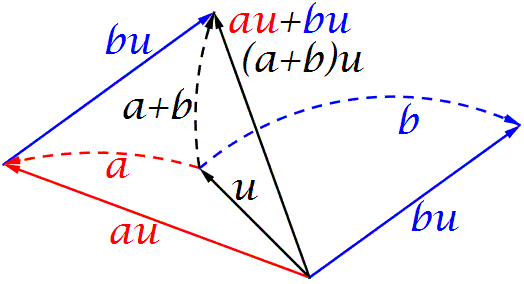
\includegraphics[width=0.5\textwidth]{imagenes/imagenes01/T01IM01.png}
		%\caption{Los dos problemas clásicos del cálculo: trazado de tangentes y áreas bajo curvas.}
	%\end{figure}
		
%varios párrafos encuadrados - explicaciones ad hoc
%\centering{
%\fbox{
%\parbox{0.95\textwidth}{
%varios
%
%$parrafos
%
%dentro
%}
%}
%}
% \justify


%\rotatebox{180}{\leftline{\textcolor{gris}{tararí}}}.



\chapter{Matrices}	

\section[Matrices: definición, tipo o dimensión e igualdad]{Matrices: definición, tipo o dimensión e igualdad} \sectionmark{Matrices. Definición}
\sectionmark{Matrices. Definición}

En adelante, $\mathbb K$ será uno de los cuerpos $\mathbb Q, \; \mathbb R, \; \mathbb C$;  $\; m$ y $n$ representarán números naturales:

\begin{defi} Una `matriz' es un tablero rectangular que contendrá elementos del cuerpo $\mathbb K$. La matriz será una colección de filas y columnas de números (aunque podían ser vectores, funciones, etc). 	
\end{defi}
\begin{defi}
Se llama `dimensión' o `tipo' de una matriz	al `número (indicado, no multiplicado)  de filas' por `número de columnas', así, una matriz de tipo $m\times n$, que representaremos por letras mayúsculas $A$, p.e., será un tablero rectangular que contendrá $m$-filas y $n$-columnas de números (que representaremos por letras minúsculas $a_{ij}$, haciendo referencia el primer índice $i$ a la fila que ocupa el elemento y el segundo índice $j$ a la columna en que está).

\begin{myblock}{Matriz $\boldsymbol{A_{m\; x \; n}}$}

$A=\left[
\begin{matrix}
a_{11} & a_{12} & \cdots & a_{1j} & \cdots & a_{1n} \\
a_{21} & a_{22} & \cdots & a_{2j} & \cdots & a_{2n} \\
a_{31} & a_{32} & \cdots & a_{3j} & \cdots & a_{3n} \\
\vdots & \vdots & \ddots & \vdots & \ddots & \vdots \\
a_{i1} & a_{i2} & \cdots & \boxed{a_{ij}} & \cdots & a_{in} \\
\vdots & \vdots & \ddots & \vdots & \ddots & \vdots \\
a_{m1} & a_{m2} & \cdots & a_{mj} & \cdots & a_{mn} \\
\end{matrix}
\right]$
\footnotesize{$= [a_{ij}]_{m \times n} \; \begin{cases}0\le i \le m; \\ 0\le j \le n\end{cases}$}

\vspace{3mm}
\centerline{$\boxed{\; \boldsymbol{A_{\;  (num. \; filas)\; \times \; (num. \; columnas) }}\; }$}

\end{myblock}

\end{defi}
 
Los elementos $a_{i1}, a_{i2}, \cdots , a_{in}$ forman la `fila i-ésima'

Los elementos $a_{1j}, a_{2j}, \cdots , a_{mj}$ forman la `columna j-ésima'

Por ejemplo: \hspace{2mm} fila-2 $\; (a_{21}, a_{22}, \cdots , a_{2n})\; $;\hspace{2mm} columna 3 $\; \left(\begin{matrix} a_{12} \\ a_{23}\\ \vdots \\ a_{m3}   \end{matrix}  \right)$. 

De este modo puede considerar a $A$ como una matriz de m-filas o de n-columnas:
$\quad A \quad=\quad \left( \begin{matrix} f_1 \\f_2\\ \vdots \\ f_m \end{matrix} \right) \quad = \quad  (\;c_1, c_2, \cdots, c_n \;)$


\begin{defi}Igualdad de matrices.

Dos matrices son iguales si, siendo del mismo tipo, tienen los mismos elementos en las misma posiciones:

$\quad { \left( { a }_{ ij } \right)  }_{ \begin{matrix} 1\le 1\le m \\ 1\le i\le n \end{matrix} }$
$\; = \; $
${ \left( { b }_{ ij } \right)  }_{ \begin{matrix} 1\le 1\le m \\ 1\le i\le n \end{matrix} } \leftrightarrow a_{ij}=b_{ij}; \; \forall i,j$

\end{defi}

En lo sucesivo llamaremos $\boldsymbol{ \mathcal M_{m\times n}(\mathbb K) }$ al conjunto de todas las matrices de tipo $m\times n$ sobre el cuerpo $\mathbb K$. Y, en general, mientras no se diga lo contrario, consideraremos $\mathbb K=\mathbb R$, hablaremos de matrices de números reales.

\subsection{Matriz traspuesta}

\begin{defi} Dada $A_{m\times n}\in \mathcal M_{m\times n}(\mathbb R)$, se llama `matriz traspuesta' de $A$ y se denota por $A^T$ a la matriz que resulta de `cambiar en $A$ las filas por las columnas' (o viceversa), es decir:

$A^T_{n\times m} = (A_{m\times n})^T\; :\;  \; $ si  $\quad$ \colorbox{LightYellow}{$\boxed{ \; A=(a_{ij}) \to A^T=(a_{ji})\; }$	}
\end{defi}

\begin{ejem}
$A_{2\times 3}=\left( \begin{matrix} 1 & 2 & 3 \\ 4 & 5 & 6 \end{matrix} \right)	 \to A^T_{3\times 2}= \left( \begin{matrix} 1 & 4 \\ 2 & 5 \\ 3 & 6 \end{matrix} \right)	 $

\noindent \small{$B_{4\times 1}=\left( \begin{matrix} 1 \\ 2 \\ 3 \\ 4 \end{matrix} \right) \to B^T_{1\times 4}= (\;1,2,3,4 \; ) \; ; \qquad C_{1\times 3}= (\;x,y,z \;) \to C^T_{3\times 1}=\left( \begin{matrix} x \\ y \\ z \end{matrix} \right)$}
\end{ejem}

\begin{prop}{Propiedad de la matriz traspuesta}
\label{propo1}

$A_{m\times n}\in \mathcal M_{m\times n}(\mathbb R) \to\; \boxed{\; \boldsymbol{ (A^T)^T=A}\; } $ 	
\end{prop}

\begin{proof}.

Evidentemente: $A=(a_{ij}) \to A^T=(a_{ji}) \Rightarrow (A^T)^T=(a_{ij})=A$	
\end{proof}


\section{Matrices especiales}

\begin{defi} `Matriz Cuadrada': son matrices del tipo $n\times n$, es decir, que tienen el `mismo número de filas que de columnas'.

Los elementos de la forma $a_{ii}$ se llaman `elementos diagonales' y a la línea en que están situados se le llama `diagonal principal'.
\end{defi}
\begin{defi}
`Matriz Diagonal' es una matriz cuadrada en la que los elementos que no están en la diagonal principal valen todos cero: $a_{ij}=0, \; \forall i \neq j$	
\end{defi}
\begin{defi} `Matriz Identidad o Unidad', es una matriz diagonal con los elementos de la diagonal ppal. iguales a uno. $a_{ii}=1; \; a_{ij}=0, \; \forall i \neq j$	
\end{defi}
 A las matrices cuadradas del tipo $A_{n \times n}$ se les suele llamar matrices cuadradas de orden-$n$.


\begin{ejem}.

 $C=\left(\begin{matrix} \boxed{1} & -2 & 3 \\-2 & \boxed{0} & 1 \\4 &-3 &\boxed{-1}  \end{matrix} \right) \quad D=\left(\begin{matrix} 1 & 0 &  0\\0 & 5 & 0 \\0 & 0 &-3  \end{matrix} \right) \quad I=\left(\begin{matrix} 1 & 0 & 0 \\0 & 1 & 0 \\0 &0 &1  \end{matrix} \right)$

\small{$C$ es una matriz cuadrada, $D$ es una matriz diagonal y $I$ es la matriz identidad, todas de orden $3$}.	 En la matriz $C$ hemos destacado en cuadros los elementos de la diagonal principal.
\end{ejem}
\begin{defi} `Matriz Triangular', es una matriz cuadrada en la que todos los elementos por encima (triangular inferior) de la diagonal principal son cero ($a_{ij}=0; \; \forall i < j$). Análogamente se define la matriz triangular superior como aquella en que los elementos por debajo la de diagonal principal son cero ($a_{ij}=0; \; \forall i > j$)	
\end{defi}
\begin{ejem}.

$M=\left( \begin{matrix} \boxed{1}&0&0\\3&\boxed{-4}&0 \\-1&3&\boxed{1}  \end{matrix}\right)\qquad N=\left( \begin{matrix} \boxed{1}&3&-1&2 \\0&\boxed{3}&2&-2\\0&0&\boxed{1}&1\\0&0&0&\boxed{-3}   \end{matrix}\right)$	

$M$ es una matriz triangular inferior y $N$ una matriz triangular superior (?`no recuerda al método de Gauss?)
\end{ejem}
\begin{defi} `Matrices Simétricas y Antisimétricas (o Hemisimétricas)'.

$S$ es una `matriz simétrica' si es una matriz cuadrada que cumple $S^T=S$, es decir $s_{ij}=s_{ji}, \; \forall i,j$

$H$ es una `matriz antisimétrica o hemisimétrica' si es una matriz cuadrada tal que $H^T=-H$, es decir, $h_{ij}=-h_{ji},\; \forall i,j$. Necesariamente ha de ocurrir que $h_{ii}=0,\; \forall i$.	
\end{defi}
\begin{ejem}
$S=\left( \begin{matrix} 1&-2&3 \\-2&5&4 \\ 3&4&7  \end{matrix}\right)	\qquad H=\left( \begin{matrix} 0&-2&5 \\2 &0& 3 \\ -5&-3&0 \end{matrix}\right)$
\end{ejem}
\begin{defi}
`Matriz Nula' es cualquier matriz, no necesariamente cuadrada, tal que todos sus elementos son cero.

$\quad A=\left( \begin{matrix} 0&0&0\\0&0&0\\0&0&0   \end{matrix}\right); \qquad B=\left( \begin{matrix} 0&0&0&0 	\\ 0&0&0&0  \end{matrix}\right); \qquad C=\left( \begin{matrix} 0\\0\\0  \end{matrix}\right), \qquad $ son matrices nulas.	
\end{defi}

\begin{defi}

\textcolor{gris}{Otras matrices especiales $\divideontimes$}

\textcolor{gris}{$A$ es una matriz `involutiva' si $A^2=A\cdot A=I$}

\textcolor{gris}{Matriz `idempotente', si $A^2=A$}

\textcolor{gris}{Matriz `nihilpotente de orden $k$', si $A^k=0,\;$ con $A^{k-1}\neq 0$}
	
\end{defi}



\section{Operaciones con matrices}

\subsection{Producto de una matriz por un escalar (número real)}

\begin{defi}
Sea $k\in \mathbb R$ y $A_{m\times n}=(a_{ij}) \in \mathcal M (\mathbb R)$, se define el `producto de un número real $k$ por una matriz $A$ como aquella matriz del mismo tipo que $A$ en que cada uno de sus elementos está multiplicado por el número $k$:
$\qquad k \cdot A= k\cdot (a_{ij})= (k\cdot a_{ij})$, más explícitamente:

\vspace{2mm} \hspace{1cm} \colorbox{LightYellow}{$\boxed{\; k \cdot \left( \begin{matrix} a_{11} & \cdots & a_{1n} \\
\vdots & \ddots & \vdots \\ a_{m1} & \cdots & a_{mn}     \end{matrix}\right)	 = \left( \begin{matrix} k\cdot a_{11} & \cdots & k\cdot a_{1n} \\
\vdots & \ddots & \vdots \\ k\cdot a_{m1} & \cdots & k\cdot a_{mn}     \end{matrix}\right)\; }$}
\end{defi}

\begin{ejem}
$-3 \cdot \left( \begin{matrix} 1&2&-2 \\0&-1&5  \end{matrix}\right)= \left( \begin{matrix} -3&-6&6\\0&3&-15  \end{matrix}\right)$	
\end{ejem}
\begin{prop}{Propiedades del producto de una matriz por un escalar}.

\begin{enumerate}
\item $k\cdot A$ es una operación externa de $\mathbb R$ sobre $\mathcal M(\mathbb R)$ (el producto de un número por una matriz es una matriz).
\item ``asociativa'': $(\lambda \cdot \mu)\cdot A= \lambda\cdot (\mu \cdot A)$
\item ``distributiva-1'': $(\lambda+\mu)\cdot A= \lambda \cdot A + \mu \cdot A$
\item ``distributiva-2'': $\lambda \cdot (A+B)= \lambda \cdot A + \lambda \cdot B$
\item ``elemeto unidad'' $1\cdot A = A$	
\end{enumerate}
\hspace{1cm}$\forall \lambda, \mu \in \mathbb R; \; \forall A,B \in \mathcal M(\mathbb R)$
	
\end{prop}
\begin{proof}
La demostración es trivial basándose en la definición.	
\end{proof}



\subsection{Suma de matrices}

\begin{defi} Sean $A_{m\times n}=(a_{ij}); \; B_{m\times n}=(b_{ij}) \in \mathcal M_{m \times n} (\mathbb R)$, dos matrices \textbf{del mismo tipo o dimensión}, llamamos matriz suma a una matriz, del mismo tipo que las anteriores, en que cada elemento se obtiene sumando los respectivos elementos de las matrices $A$ y $B$, es decir:

$A+B=(a_{ij})+(b_{ij})=(a_{ij}+b_{ij})$, más explícitamente:

\vspace{2mm} $A+B=\;$  \colorbox{LightYellow}{$\boxed{ \; \left( \begin{matrix}  a_{11} & \cdots &  a_{1n} \\
\vdots & \ddots & \vdots \\ a_{m1} & \cdots &  a_{mn}     \end{matrix}\right)+ 
\left( \begin{matrix}  b_{11} & \cdots &  b_{1n} \\
\vdots & \ddots & \vdots \\  b_{m1} & \cdots &  b_{mn}     \end{matrix}\right)\; =\; }$} 

\hspace{1cm} \colorbox{LightYellow}{$\boxed{\; =\left( \begin{matrix}  a_{11}+b_{11} & \cdots &  a_{1n}+b_{1n} \\
\vdots & \ddots & \vdots \\  a_{m1}+b_{m1} & \cdots &  a_{mn}+b_{mn}     \end{matrix}\right)\;}$ } $\; =A+B$

`Solo se pueden sumar matrices del mismo tipo o dimensión'
\end{defi}
\begin{ejem}
$A+B=\left( \begin{matrix} 2&3 \\-1&1\\0&2\\3&-1   \end{matrix}\right) +
\left( \begin{matrix} 1&-1\\1&0\\0&3\\-4&2  \end{matrix}\right)=
\left( \begin{matrix}3&2\\0&1\\0&5\\-1&1   \end{matrix}\right)$	
\end{ejem}
\begin{prop}{Propiedades de la suma de matrices}
\begin{enumerate}
	\item $+$ es una operación interna en $\mathcal M(\mathbb R)$ (la suma de matrices $m\times n$ es una matriz $m \times n$).
	\item asociativa: $A+(B+C)=(A+B)+C$
	\item conmutativa: $A+B=B+A$
	\item matriz nula (neutro) : $A+0=A$
	\item matriz opuesta: $A+(-A)=0 \to (-A)=(-1)\cdot A=-A$
	
\end{enumerate}
\hspace{1cm} $\forall A,B,C \in \mathcal M(\mathbb R)$; $0=0_{m\times n}$ es la matriz nula.

\hspace{1cm}\textcolor{gris}{$\divideontimes \quad \left( \mathcal M_{m\times n}(\mathbb R),+ \right) $ es un grupo abeliano.}
\end{prop}
\begin{proof}
La demostración es trivial basándose en la definición.	
\end{proof}


\subsection{Producto de matrices}

\begin{defi}
`Producto de una matriz fila (de $n$-elementos) por una matriz columna (de $n$-elementos)'.

$A_{1\times \cancel{n}}\cdot B_{\cancel{n}\times 1} = P_{1\times 1} \; : \; \; $

\noindent  \colorbox{LightYellow}{$\boxed{\; \left( \begin{matrix} a_1, \; a_2, \; \cdots, \; a_n   \end{matrix}\right)  \cdot  
\left( \begin{matrix} b_1 \\ b_2 \\ \vdots \\ b_n  \end{matrix}\right) = (\;a_1 b_1+ a_2 b_2 + \cdots + a_n b_n \; )\; }$} \tiny{$ \in \mathcal M_{1 \times 1}(\mathbb R)=\mathbb R$}\normalsize{.} 
\end{defi}
\begin{ejem}.

\small{$\left( \begin{matrix} 1, 2, 3, 4   \end{matrix}\right)_{1 \times \boldsymbol{4}} \cdot \left( \begin{matrix} -1 \\ 0 \\ 2  \end{matrix}\right)_{\boldsymbol{3} \times 1}$, no tiene sentido, en cambio:}

\small{$\left( \begin{matrix} 1, 2, 3, 4   \end{matrix}\right)_{1\times \cancel{4}}\cdot \left( \begin{matrix} -1 \\ 0 \\ 2 \\5 \end{matrix}\right)_{\cancel{4} \times 1}= (\; 1\cdot (-1)+ 2 \cdot 0 + 3 \cdot 2 + 4 \cdot 5\;)= $}

\small{$=(\; -1+0+6+20\; ) = (\; 25 \; )_{1\times 1}$}
\end{ejem}
\begin{defi}`Producto de una matriz $m \times \boldsymbol{p}$ por una matriz $\boldsymbol{p} \times n$'

$A_{m\times p} \cdot B_{p\times n}$, el resultado es una matriz $P$, de dimensión  $(\boldsymbol{m} \times \cancel{p})\;  \cdot \; (\cancel{p} \times \boldsymbol{n})\; =\; \boldsymbol{(m \times n)} $, en que cada elemento $p_{ij}$ de la matriz producto $P$ se obtiene como producto de la fila-$i$ de la matriz $A$ por la columna-$j$ de la matriz $B$. 

 \colorbox{LightYellow}{$\boxed{\displaystyle \; A_{m\times p} \cdot B_{p\times n}=P_{m \times n}\; / \; p_{ij}=f_i(A)\cdot c_j(B)}$} $\;= (\divideontimes)\; \sum_{k=1}^{p}{a_{ik}\; b_{kj}}\; $

De otro modo, si $A=\left( \begin{matrix} \boxed{a_{11}} &\boxed{\cdots} & \boxed{a_{1p}}\\
\vdots & \ddots & \vdots \\ a_{m1} & \cdots & a_{mp}   \end{matrix}\right)=
\left( \begin{matrix} f_1(A) \\ \vdots \\ f_m(A)  \end{matrix}\right)$ y 

$B=\left( \begin{matrix} \boxed{b_{11}} &\cdots & a_{1n}\\
\boxed{\vdots} & \ddots & \vdots \\ \boxed{b_{p1}} & \cdots & b_{pn}   \end{matrix}\right)=
\left( \begin{matrix} \;  c_1(A),\; \cdots ,\; c_n(B)\;   \end{matrix}\right) \; \; \Rightarrow$

$A\cdot B= P = \left( \begin{matrix} \boxed{f_1(A)\; c_1(B)} & \cdots &\;  f_1(A)\; c_n(B) \\
\vdots & \ddots & \vdots \\
f_m(A)\; c_n(B) & \cdots & f_m(A) \; c_n(B) \; c  \end{matrix}\right)$

	\begin{figure}[]
		\centering
		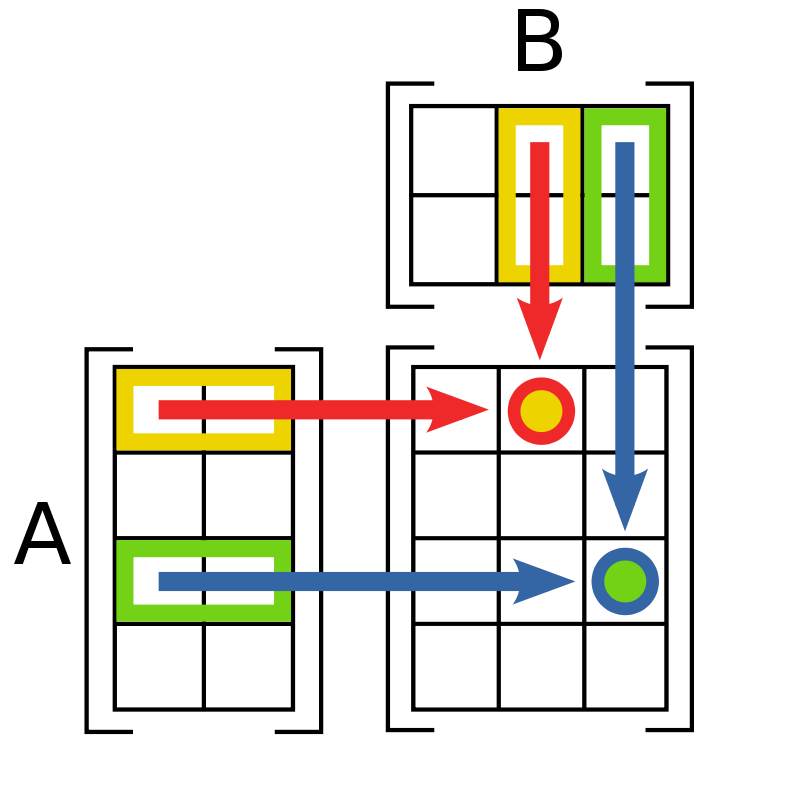
\includegraphics[width=0.5\textwidth]{imagenes/imagenes03/T03IM01.png}
		\caption{Productos de matrices \footnotesize\textit{{(fuente: Wikipedia)}}}
	\end{figure}

\end{defi}
\begin{ejem}.

$A_{3\times 2}=	\left( \begin{matrix}  1&1\\0&-2\\3&4 \end{matrix}\right); \quad 
B_{2\times 4}=\left( \begin{matrix}  1&1&0&-1 \\ 3&3&-1&2 \end{matrix}\right); \quad 
C_{2\times 2}=\left( \begin{matrix}  1&2\\3&4 \end{matrix}\right)$

Calcula, si es posible: 

$A\cdot B; \; A\cdot C; \; B\cdot A;\; B\cdot C;\; C\cdot A; \; C\cdot B; \; A\cdot A; \; B\cdot B; \; C\cdot C $

%\rule{50mm}{0.2pt}

\noindent $A_{3x2}\cdot B_{2x4}=$
\small{$AB_{3x4}=\left( \begin{matrix}  \boxed{1}&\boxed{1}\\0&-2\\3&4 \end{matrix}\right) \cdot \left( \begin{matrix}  \boxed{1}&1&0&-1 \\ \boxed{3}&3&-1&2 \end{matrix}\right)$}\normalsize{$=$}
$\left( \begin{matrix} \boxed{4}&4&-1&1\\-6&-6&2&-4\\15&15&-4&5  \end{matrix}\right)$

\noindent $A_{3x2}\cdot C_{2x2}=AC_{3x2}=$
\small{$\left( \begin{matrix}  1&1\\\boxed{0}&\boxed{-2}\\3&4 \end{matrix}\right) 
\cdot  \left( \begin{matrix}  1&\boxed{2}\\3&\boxed{4} \end{matrix}\right)$}\normalsize{$=$}
$\left( \begin{matrix} 4&6\\-6&\boxed{8}\\15&14  \end{matrix}\right)$

\noindent $\nexists B_{4x2}\cdot A_{3x2}; \quad \nexists B_{4x2}\cdot C_{2x2}; \quad \nexists C_{2x2}\cdot A_{3x2}$

\noindent $C_{2x2}\cdot B_{2x4}=CB_{2x4}$
\small{$=\left( \begin{matrix}  1&2\\\boxed{3}&\boxed{4} \end{matrix}\right) \cdot
\left( \begin{matrix}  1&1&\boxed{0}&-1 \\ 3&3&\boxed{-1}&2 \end{matrix}\right)$}\normalsize{$=$}
$\left( \begin{matrix} 7&7&-2&3\\15&15&\boxed{-4}&5  \end{matrix}
\right)$

\noindent $\nexists A_{3x2} \cdot A_{3x2}; \quad \nexists B_{2x4} \cdot B_{2x4}$

\noindent $C_{2x2} \cdot C_{2x2}=C^2_{2x2}=$
\small{$\left( \begin{matrix}  1&2\\\boxed{3}&\boxed{4} \end{matrix}\right)\cdot \left( \begin{matrix}  1&\boxed{2}\\3&\boxed{4} \end{matrix}\right)$}\normalsize{=}
$\left( \begin{matrix}  7&10\\15&\boxed{22} \end{matrix}\right)$

En este último caso hemos destacado el elemento $2,2$ de $C^2$ como proveniente de multiplicar la fila $2$ de $C$ por la columna $2$ de C. En los otros casos hemos destacados otros elementos a fin de aclarar el producto de matrices. 

\emph{Asegúrese el/la lector/a de que sabe multiplicar matrices antes de continuar}.
\end{ejem}

\begin{prop}{Propiedades del producto de matrices}

\begin{enumerate}

\item El producto de matrices es asociativo: $A\cdot(B\cdot C)=(A\cdot B)\cdot C$
\item !`El producto de matrices es \textbf{no conmutativo}!:  \colorbox{LightYellow}{$\boxed{ \; A\cdot B \neq B\cdot A \; }$}

\vspace{2mm}
$A\cdot B$ puede existir y $B\cdot A$ no. Incluso si existen ambos productos, no tiene por que coincidir. Piénsese en las matrices: $X_{3x1}; \; Y_{1x3}; \; Z_{3x3}$. En que $\exists (ZX)_{3x1}$ pero $\nexists XZ$. Incluso en el caso en que existan ambas, $(XY)_{3x3}\neq (YX)_{1x1}$

Es por ello muy \textbf{importante el orden en que se multiplican las matrices}, llegando a hablar de la matriz que `premultiplica o va delante' y la matriz que `postmultiplica o va detrás'.

\item Distributivas: $\begin{cases} \; A\cdot (B+C)=A\cdot B + A\cdot C \\  \; (A+B)\cdot C=A\cdot C+ B\cdot C   \end{cases}$


\vspace{2mm} !`OJO al orden en que se multiplican las matrices!	


\item Neutro: Matriz Identidad $I_{p\times p}=(i_{kl}) \begin{cases} \; 1 \text{ si } k=l \\ \; 0 \text{ si } k\neq l \end{cases} =$ 
\small{$\left( \begin{matrix} 1 & \cdots & 0 \\ \vdots & \ddots & \vdots \\ 0 & \cdots & 1  \end{matrix}\right)_{p\times p}$}\normalsize{.}

$\forall A_{m \times n}, \; I{n\times n} \therefore \;  A\cdot I=A \quad \wedge \quad \forall A_{m \times n}, \; I{m\times m} \therefore \;  I\cdot A=A $

\item Inversa: esta propiedad, debido a su relevancia, se estudiará en el siguiente apartado.

\vspace{3mm} \textcolor{gris}{$\divideontimes \; (\mathcal M_{n}(\mathbb R) , + , \cdot)\; $ tiene estructura de anillo conmutativo.}
\end{enumerate}
	
\end{prop}
\begin{proof}
La demostración excede de los objetivos del presente texto, por lo que se verá una `comprobación' de las propiedades enunciadas en el  teorema en el apartado de ejercicios.	
\end{proof}

	\begin{figure}[H]
		\centering
		
\includegraphics[width=.8\textwidth]{imagenes/imagenes03/T03IM04.png}
	\end{figure}



\begin{coro}
Debido a la `no-conmutatividad' del producto de matrices no se cumplen las llamada identidades notables:

$(A\pm B)^2 \neq A^2 \pm 2 AB + B^2 \quad \wedge \quad (A+B)\cdot (A-B) \neq A^2 - B^2$
\end{coro}
\begin{proof}

Efectivamente: $(A+B)^2=(A+B)\cdot (A+B)=A^2+AB+BA+B^2 \neq A^2 +2AB+ B^2$, puesto que $AB\neq BA$. Lo mismo ocurre con el cuadrado de la resta.

Del	mismo modo: $(A+B)\cdot (A-B)=A^2-AB+BA-B^2 \neq A^2-B^2$, puesto que $AB\neq BA$.  
\end{proof}


\subsection{Potencias de matrices cuadradas}

\begin{defi}
Dada $A\in \mathcal M_n \to A^2=A_{n \times n} \cdot A_{n \times n} =A^2_{n \times n} $

$A^3= \begin{cases}A^2\cdot A=(A\cdot A )\cdot A  \\ A \cdot A^2 = A\cdot (A \cdot A)\end{cases}$	

Evidentemente, las sucesivas potencias de una matriz cuadrada conmutan, es decir, podemos calcular $A^8=A^5 \cdot A^3$ o $A^3\cdot A^5$.

\noindent \small{Así, en general, podríamos definir (`por inducción' - ver apéndice \ref{inducción})} $A^n=A\cdot A \cdots \cancelto{n \text{ veces }}{.}  \cdot A$\normalsize{.}
\end{defi}

\begin{ejem}
Calcula las potencias enésimas de: 

$M=\left( \begin{matrix} 1&2\\0&1 \end{matrix} \right) \quad N=\left( \begin{matrix} 1&1/5&1/5 \\ 0&1&0 \\ 0&0&1 \end{matrix} \right)$

$M=\left( \begin{matrix} 1&2\\0&1 \end{matrix} \right) \to M^2=MM=\left( \begin{matrix} 1&2\\0&1 \end{matrix} \right) \cdot \left( \begin{matrix} 1&2\\0&1 \end{matrix} \right) =\left( \begin{matrix} 1&4\\0&1 \end{matrix} \right) \to M^3=M^2\cdot M= \left( \begin{matrix} 1&6\\0&1 \end{matrix} \right) \to M^4=\left( \begin{matrix} 1&8\\0&1 \end{matrix} \right) \Rightarrow  \; M^n=\left( \begin{matrix} 1&2n\\0&1 \end{matrix} \right)\;  $ 

Realmente, hemos obtenido una `conjetura'. Ahora deberíamos someterla a la prueba del `método de inducción completa'.

$N=\left( \begin{matrix} 1&1/5&1/5 \\ 0&1&0 \\ 0&0&1 \end{matrix} \right) \to N^2=\left( \begin{matrix} 1&2/5&2/5 \\ 0&1&0 \\ 0&0&1 \end{matrix} \right) \to N^3=\left( \begin{matrix} 1&3/5&3/5 \\ 0&1&0 \\ 0&0&1 \end{matrix} \right)\to N^4=\left( \begin{matrix} 1&4/5&4/5 \\ 0&1&0 \\ 0&0&1 \end{matrix} \right) \Rightarrow \; N^n=\left( \begin{matrix} 1&n/5&n/5 \\ 0&1&0 \\ 0&0&1 \end{matrix} \right)\; $

De nuevo, este resultado solo es una conjetura.
	
\end{ejem}


\subsection{Matriz Inversa}

\begin{defi}

Dada $A\in \mathcal M_{n\times n} (\mathbb R)$, una matriz cuadrada, puede que exista otra matriz cuadraba $B_{n\times n}$ de modo que:

$A_{n\times n}\cdot B_{n \times n}= B_{n\times x}\cdot A_{n \times n}=I_n$, con $I_n=I_{n\times n}$, la identidad de orden $n$.

Si esto ocurre, si $\exists B$, decimos que $B$ es la inversa de $A$ y la representamos por $A^{-1}$, es decir:




\begin{myblock}{Matriz inversa}
\vspace{2mm} $\forall A\in \mathcal M_{n\times n} (\mathbb R), \; \text{ si } \exists A^{-1}\in \mathcal M_{n\times n} (\mathbb R) \; \therefore \; $

\vspace{3mm} \centerline{$\boxed{\; A\cdot A^{-1}=A^{-1}\cdot A=I\; }\; $,} 

\vspace{2mm} decimos que $A$ es `invertible o regular' y que $A^{-1}$ es su matriz inversa. 
\end{myblock}

\end{defi}

\noindent \textbf{Observaciones:}

Para tener matriz inversa, la matriz de partida ha de ser cuadrada. Pero no todas las matrices cuadradas tienen inversa. Cuando una matriz cuadrada no tiene inversa de dice que es una `matriz singular o no invertible'.

Por ejemplo, la matriz $\left( \begin{matrix} 1&0\\0&0  \end{matrix}\right)$ es singular, pues no existe ninguna matriz $\left( \begin{matrix} a&b\\c&d  \end{matrix}\right)$ tal que $ \left( \begin{matrix} 1&0\\0&0  \end{matrix}\right)\cdot \left( \begin{matrix} a&b\\c&d  \end{matrix}\right)  =\left( \begin{matrix}1&0\\0&1   \end{matrix}\right)=I$ (\textit{Compruébese resolviendo el SEL})

En el próximo capítulo, `Determinantes', veremos un teorema que asegura cuando una matriz cuadrada tiene o no inversa.

\subsection{Propiedades interesantes de las operaciones con matrices}

\begin{lema}
\label{lema1}\label{producto-traspuestas}

$(A+B)^T=A^T + B^T\; $ La traspuesta de la suma de matrices es la suma de matrices traspuestas.
\end{lema}
\begin{proof}

Sea $A_{m\times n}=(a_{ij}); \; B_{m \times n}=(b_{ij}) \to A^T=(a_{ji})\; \wedge \; B^T=(b_{ji})$

Como $A+B=	(a_{ij}+b_{ij}) \to (A+B)^T=(a_{ji}+b_{ji})=(a_{ji}) + (b_{ji})=B^T+A^T$ 

\end{proof}



\begin{teor}
$\divideontimes \; \; $ Toda matriz cuadrada $M$ se puede descomponer como suma de dos matrices cuadradas $S$ y $H$, una de ellas simétrica y la otra antisimétrica.	
\end{teor}
\begin{proof}
Basta con considerar $S=\frac 1 2 (M+M^T)$ y $H=\frac 1 2 (M-M^T)$

En efecto, $S+T = \frac 1 2 [ (M+M^T)+(M-M^T)]= \frac 1 2 2M= M$

Además, $S^T = \frac 1 2 (M+M^T)^T=\frac 1 2 (M^T+M)=S\; $ Simétrica.

Y, $\; H^T=\frac 1 2 (M-M^T)^T=\frac 1 2 (M^T-M)=-\frac 1 2 (M-M^T)=-H\;$, Antisimétrica.

Hemos usado para demostración la proposición \ref{propo1} ($(A^T)^T=A)$) y el lema anterior \ref{lema1}.
\end{proof}
\begin{teor}
$\divideontimes \; \; $ La traspuesta del producto de dos matrices cuadradas es igual al producto de las matrices transpuestas, pero con el orden de multiplicación invertido. $(\; A\cdot B)^T=B^T \; \cdot \; A^T$ 	
\end{teor}
\begin{proof}

La demostración es más complicada en este caso, así que, para mayor claridad en la exposición, nos contentaremos con una `comprobación' para un caso particular, que no es ninguna demostración pero será suficiente para los objetivos de este libro. 	

$A=\left( \begin{matrix} 1&0 \\ 2&-1   \end{matrix}\right); \qquad B=\left( \begin{matrix} 3&-2&1&0 \\-2&1&1&-1  \end{matrix}\right)$


$A\cdot B=\left( \begin{matrix} 1&0 \\ 2&-1  \end{matrix}\right) \cdot  \left( \begin{matrix} 3&-2&1&0\\-2&1&1&-1  \end{matrix}\right) = \left( \begin{matrix} 3&2&-1&0\\8&-5&1&1 \end{matrix}\right) \to$

$ (AB)^T=\; \left( \begin{matrix} 3&8\\2&-5\\-1&1\\0&1 \end{matrix}\right)\; $

$B^T\cdot A^T=\left( \begin{matrix} 3&-2\\-2&1\\1&1\\0&-1 \end{matrix}\right) 
\cdot \left( \begin{matrix} 1&2\\0&-1  \end{matrix}\right)=
\; \left( \begin{matrix}   3&8\\2&-5\\-1&1\\0&1 \end{matrix}\right)\; $


Destacar que está curiosa propiedad (se alterna el orden) ya vimos que se cumplía con una operación no-conmutativa como la composición de funciones y el cálculo de la función inversa: $(f \circ g)^{-1}= g^{-1} \circ f^{-1}$

\end{proof}
\begin{teor}
\label{prod-inv}
$\divideontimes \; \;$ La inversa del producto de dos matrices es igual al producto de las matrices inversas, pero con el orden de multiplicación invertido. $ \; (A\cdot B)^{-1}=B^{-1} \; \cdot \; A^{-1}$ 	


	
\end{teor}
\begin{proof}

De modo análogo al teorema anterior, la demostración excede a los objetivos de este curso y solo haremos una mera comprobación que veremos en el apartado de ejercicios, después de aprender a calcular matrices inversas por el método de Gauss.

De nuevo se cumple la curiosa propiedad antes comentada.


\end{proof}

\begin{teor}
	$(A^{-1})^{-1}=A\; \qquad (A^T)^{-1}=(A^{-1})^T$
\end{teor}
\begin{proof}
El mismo comentario que en el teorema anterior, veremos `comprobaciones' en ls ejercicios.	
\end{proof}




\section{Método de Gauss para el cálculo de $A^{-1}$}


Supongamos que la matriz tiene inversa $\; A= \left( \begin{matrix}  a_{11}&a_{12}&\cdots &a_{1n}\\ a_{21}&a_{22}&\cdots &a_{2n}\\ \vdots&\vdots&\ddots&\vdots\\a_{n1}&a_{n2}&\cdots &a_{nn}  \end{matrix} \right)$

El método de Gauss-Jordan consiste, esquemáticamente en colocar en la misma matriz a $A$, una barra separadora y detrás a la matriz $I$. Conseguir, mediante transformaciones de Gauss que primero por debajo de la diagonal principal y después por arriba de ésta, todos los elementos que habían en $A$ sean ceros, diagonalizar la matriz $A$ mediante transformaciones de Gauss. Luego, dividiendo cada fila por la cantidad correspondiente, obtener, donde estaba $A$, que esté la matriz Identidad $I$. Si ello ha sido posible, la matriz que haya quedado detrás de la barra inicial será la matriz inversa $A^{-1}$.

Lo que no está permitido ahora /en SEL sí lo estaba) es cambiar de posición ni filas ni columnas.

El método de Gauss permite obtener $A^{-1}$ si ello es posible, si no lo es se llega a un paso a partir del cual no se puede continuar el proceso, por ello, no es éste el mejor método para el cálculo de inversas pero no podremos usar un método mejor (por `adjuntos') hasta que desarrollemos el siguiente tema de determinantes.

\vspace{3mm}

\centerline{$\colorbox{LightYellow}{\boxed{ \; \; [\; A \; | \; I \; ] \; \to \text{ transf. Gauss } \to  \; [\; I \; | \; \boldsymbol{ A^{-1} } \; ] \; \; }}$}
\justify


$\left[ \begin{matrix}  a_{11}&a_{12}&\cdots &a_{1n}\\ a_{21}&a_{22}&\cdots &a_{2n}\\ \vdots&\vdots&\ddots&\vdots\\a_{n1}&a_{n2}&\cdots &a_{nn}  \end{matrix} \right|
 \left. \begin{matrix} 1&0&\cdots&0\\ 0&1&\cdots&0\\  \vdots&\vdots&\ddots&\vdots \\0&0&\cdots&1    \end{matrix}   \right] \to
  \left[ \begin{matrix} 1&0&\cdots&0\\ 0&1&\cdots&0\\  \vdots&\vdots&\ddots&\vdots \\0&0&\cdots&1    \end{matrix}   \right|
  \left. \begin{matrix} * & * & \cdots & * \\  * & * & \cdots & * \\  \vdots&\vdots&\ddots&\vdots    \\ * & * & \cdots & * \\   \end{matrix} \right]$


Si se ha conseguido escribir delante la matriz $I$, la matriz que figura detrás (*) será la inversa de $A$, $\; A^{-1}$

\begin{ejem}
Calcula, si es posible, las siguientes matrices inversas:

$A=\left[\begin{matrix} 4&-2\\2&1  \end{matrix}\right]; \quad 
B=\left[\begin{matrix} 1&0&2\\3&1&-1\\-2&1&5  \end{matrix}\right] \quad 
C=\left[\begin{matrix} 4&6\\2&3  \end{matrix}\right]$

%\vspace{2mm}
\rule{5cm}{0.2pt}

%\vspace{2mm}

--- Inversa de A:

$A=\left[\begin{matrix} 4&-2\\2&1  \end{matrix}\right|
\left. \begin{matrix}1&0\\0&1\end{matrix} \right] \to (\; F2\to 2F2-F1\;) \to 
\left[\begin{matrix} 4&-2\\0&4  \end{matrix}\right|
\left. \begin{matrix}1&0\\-1&2\end{matrix} \right] \to 
(\;F1\to 2F1+F2 \;) \to 
\left[\begin{matrix} 8&0\\0&4  \end{matrix}\right|
\left. \begin{matrix}1&2\\-1&2\end{matrix} \right] \to \begin{cases} \; F1\to F1/8 \\ F2\to F2/4\end{cases} \to $

$\to \left[\begin{matrix} 1&0\\0&1  \end{matrix}\right|
\left. \begin{matrix}1/8&1/4\\-1/4&1/2\end{matrix} \right]$ Como delante está $I \Rightarrow $

$A^{-1}=\left[ \begin{matrix}1/8&1/4\\-1/4&1/2\end{matrix} \right]=\dfrac 1 8 \left[ \begin{matrix}1&2\\-1&4\end{matrix} \right]$

Comprobémoslo: $A\cdot A^{-1} = I = A^{-1}\cdot A$:

$A\cdot A^{-1} = \left[\begin{matrix} 4&-2\\2&1  \end{matrix}\right] \cdot \dfrac 1 8 \left[ \begin{matrix}1&2\\-1&4\end{matrix} \right] = $
$\dfrac 1 8 \left [ \begin{matrix} 8&0\\0&8 \end{matrix} \right]=I$


$A^{-1} \cdot A =   \dfrac 1 8 \left[ \begin{matrix}1&2\\-1&4\end{matrix} \right] \cdot \left[\begin{matrix} 4&-2\\2&1  \end{matrix}\right]=$
$\dfrac 1 8 \left [ \begin{matrix} 8&0\\0&8 \end{matrix} \right]=I$

Luego, efectivamente, la inversa de $A$ es: $ \; A^{-1}=\dfrac 1 8 \left[ \begin{matrix}1&2\\-1&4\end{matrix} \right] \; $

--- Inversa de B:




\noindent \small{
$\left[\begin{matrix} 1&0&2\\3&1&-1\\-2&1&5  \end{matrix}\right|
\left. \begin{matrix} 1&0&0 \\ 0&1&0 \\0&0&1  \end{matrix} \right] \to \begin{cases} F2\to F2+2F1 \\ F3\to F3-3F1   \end{cases} \to $	
$\left[\begin{matrix} 1&0&2\\0&1&-7\\0&1&9  \end{matrix}\right|
\left. \begin{matrix} 1&0&0 \\ -3&1&0 \\2&0&1  \end{matrix} \right] \to $}

\noindent \small{$(\;F3\to F3-F2 \; )  \to 
\left[\begin{matrix} 1&0&2\\0&1&-7\\0&0&16  \end{matrix}\right|
\left. \begin{matrix} 1&0&0 \\ -3&1&0 \\5&-1&1  \end{matrix} \right] \to 
\begin{cases}\; F1\to 8F1-F3 \\ \; F2\to 16F2+7F3  \end{cases}\to  $}

\noindent \small{$  \to   
\left[\begin{matrix} 8&0&0\\0&16&0\\0&0&16  \end{matrix}\right|
\left. \begin{matrix} 3&1&-1 \\ -13&9&7 \\5&-1&1  \end{matrix} \right]
* \; (F1\to 2F1) \;  *  
\left[\begin{matrix} 16&0&0\\0&16&0\\0&0&16  \end{matrix}\right|
\left. \begin{matrix} 6&2&-2 \\ -13&9&7 \\5&-1&1  \end{matrix} \right]
$}  

\normalsize{Como delante, previo a dividir por $16$ cada una de las filas, aparecerá la matriz identidad, la matriz de atrás es la inversa de B}:

\hspace{15mm} $\; B^{-1}= \dfrac 1 {16} \left[ \begin{matrix} 6&2&-2 \\ -13&9&7 \\5&-1&1  \end{matrix} \right]\; $

Compruébese que realmente se trata de la inversa de $B$, calculando: $B\cdot B^{-1}=B^{-1}\cdot B=I$

--- Inversa de C:

$\left[\begin{matrix} 4&6\\2&3  \end{matrix}\right|
\left.\begin{matrix} 1&0\\0&1  \end{matrix}\right] \to (F2\to 2F2-F1) \to 
\left[\begin{matrix} 4&\boxed{6}\\0&0  \end{matrix}\right|
\left.\begin{matrix} 1&0\\-1&2  \end{matrix}\right]$

\noindent \small{Es imposible combinar la $F1$ con la $F2$ para conseguir que $c_{12}=0 \to \; \nexists \;  C^{-1} \; $}\normalsize{.} 
\end{ejem}


\newpage %****************************************************
\section{Aplicaciones de las matrices}


\begin{myexampleblock}{Aplicaciones de las matrices}
	
Una vez que ya conocemos a fondo las matrices, puesto que hemos visto los distintos tipos que hay y las operaciones que podemos realizar con ellas. Vamos a ver sus aplicaciones, ya que las matrices son una herramienta muy útil no sólo en el campo de las matemáticas y la física como era de esperar; sino también en el campo de las ciencias sociales, por ejemplo en economía y en geografía. Esta gran utilidad se debe a que las matrices aportan un nuevo lenguaje facilitando el trabajo en una gran cantidad de ámbitos.

Empezaremos en primer lugar con las aplicaciones en \textbf{Matemáticas}, donde vamos a distinguir las aplicaciones en las distintas ramas:

--- Álgebra lineal: 

1. En esta rama destaca la utilidad en la resolución de sistemas de ecuaciones de la forma AX = B, mediante el cálculo de la matriz inversa (siguiente tema $\; X=A^{-1}\cdot B\; $).

2. Estudio de las aplicaciones lineales entre dos espacios vectoriales mediante la matriz asociada, que nos permite calcular el núcleo y la imagen (temas siguientes de ampliación de conocimientos $\divideontimes$).

---Análisis:

$\divideontimes$ En la rama del análisis se utilizan las matrices jacobianas, que se usan para expresar las derivadas parciales de una función en varias variables. Si f(x,y,z) está definida de la siguiente forma: 

$f:\mathbb R^2 \to \mathbb R^3 \Rightarrow J=\left(\begin{matrix} \dfrac{\partial f_1}{\partial x}  &\dfrac{\partial f_1}{\partial y}&\dfrac{\partial f_1}{\partial z} \\ \dfrac{\partial f_2}{\partial x} &\dfrac{\partial f_2}{\partial y} &\dfrac{\partial f_3}{\partial z}  \end{matrix}\right)$

--- Probabilidad: 

Cadenas de Markov: un tipo especial de proceso estocástico discreto en el que la probabilidad de que ocurra un evento depende solamente del evento inmediatamente anterior.

--- En teoría de grafos las matrices son de gran utilidad y tienen aplicaciones en diversas ramas del conocimiento humano (demografía, sociología, etc.)


Continuamos con las aplicaciones en la \textbf{Física}. (Relatividad Especial $\divideontimes$) La aplicación más importante en este campo son las transformaciones de Lorentz, que dan las ecuaciones del movimiento de un punto en línea recta y sobre el plano conocida la velocidad de la luz.

Por ejemplo: suponiendo que el punto se desplaza sobre el eje $OX$ y que estamos en un espacio tetradimensional, donde la cuarta dimensión es el tiempo, entonces, el punto tendrá como coordenadas iniciales $(x,y,z,t)$ y como finales $(x’,y’,z’,t’)$. Las ecuaciones que dan esta transformación son:

$\left( \begin{matrix} x', \; t'  \end{matrix} \right) =$
$\left( 
\begin{matrix}  \dfrac {1}{\sqrt{1- \left( \dfrac v c \right)^2}}  &\dfrac {-v}{\sqrt{1- \left( \dfrac v c \right)^2}}  \\ \dfrac {-v/c^2}{\sqrt{1- \left( \dfrac v c \right)^2}} &\dfrac {1}{\sqrt{1- \left( \dfrac v c \right)^2}} \end{matrix}
 \right)$
$ \cdot \left( \begin{matrix}  x \\ t \end{matrix} \right); \; \quad y'=y; \; z'=z$

Donde c representa la velocidad de la luz.


Una vez que ya hemos visto algunas de las aplicaciones más importantes en Ciencias, vamos a ver la importancia que tienen en las \textbf{Ciencias Sociales}, como la \textbf{Economía.}

Las matrices se utilizan para la presentación de datos de un problema en forma de tabla de doble entrada. Un ejemplo de esto es el modelo Input-Output, que permite solucionar problemas macroeconómicos (matriz de Leontiev), algunos de los cuáles son: orientar o estructurar los sectores productivos, poder predecir las demandas de producción, interpretar las relaciones económicas existentes entre los distintos sectores de producción.

Si continuamos por la Geografía, también aparecen cuando hay tablas de doble entrada, por ejemplo, para hacer referencia a la distancia que hay entre varias ciudades. En comunicaciones aéreas, para ver las distintas formas de interconectar vuelos entre diferentes paises. Etc.

\end{myexampleblock}






\begin{figure}[H]
	\centering
	
\includegraphics[width=1\textwidth]{imagenes/imagenes03/T03IM02.png}
\end{figure}









\section {Ejercicios}
\subsection {Ejercicios resueltos}

\begin{ejre}
	Escribe una matriz cuadrada de orden $3$ cuyos elementos cumplan: $\begin{cases}  2j-i & \text{ si } \textcolor{blue}{i \le j} \\ (-1)^{i+j} & \text{ si } \textcolor{red}{i>j}  \end{cases}$
\end{ejre}

\begin{proofw}\renewcommand{\qedsymbol}{$\diamond$}

\hspace{10mm}$\left( 
\begin{array}{ccc} \textcolor{blue}{a_{11}} & \textcolor{blue}{a_{12}} & \textcolor{blue}{a_{13}} \\
 \textcolor{red}{a_{21}} & \textcolor{blue}{a_{22}} & \textcolor{blue}{a_{23}} \\
\textcolor{red}{a_{31}} & \textcolor{red}{a_{32}} & \textcolor{blue}{a_{33}}
\end{array} \right) 
\to \; \left( \begin{array} {ccc}
1 &3 &5 \\-1 & 2 & 4 \\ 1 & -a & 3  	
\end{array} \right)$

	
\end{proofw}


\begin{ejre}
Considera las matrices:  

$ M=\left( \begin{matrix} 1&-1&2\\-2&0&3  \end{matrix} \right)\; \quad  N=\left( \begin{matrix} 3&-1&0\\1&2&1  \end{matrix} \right)\; \quad  P=\left( \begin{matrix}  2&-1\\3&1\\-2&0 \end{matrix} \right)$

\noindent Calcula: 
$\; \; a) \; M+N \quad b)\; \frac 2 5 N; \quad c)\; -M; \quad d)\; \frac 1 2 M - 3 N$
 
 $e)\; 2M-3P^T; \quad f)\; 3(N^T+P)-M^T\quad g)\; MP \neq PM$

 $ h) (MN^T)P^T=M(N^TP^T); \quad i) \; P(M+N)=PM+PN$

 $j)\; (MP)^T=P^TM^T; \quad i)\; MI=M \text { y } IM=M $
\end{ejre}
\begin{proofw}\renewcommand{\qedsymbol}{$\diamond$}

--- a) $M+N=\left( \begin{matrix} 1&-1&2\\-2&0&3  \end{matrix} \right)\; + \;\left( \begin{matrix} 3&-1&0\\1&2&1  \end{matrix} \right) = 
\left( \begin{matrix} 4&-2&2\\-1&2&4  \end{matrix} \right)$

\noindent --- b) $\frac 2 5 N = \frac 2 5 \; \left( \begin{matrix} 3&-1&0\\1&2&1  \end{matrix} \right) =\left( \begin{matrix} 6/5&-2/5&0\\2/5&4/5&2/5  \end{matrix} \right)$

\noindent --- c) $-M=-\; \left( \begin{matrix} 1&-1&2\\-2&0&3  \end{matrix} \right) =\left( \begin{matrix} -1&1&-2\\2&0&-3  \end{matrix} \right)$

\noindent --- d) $\frac 1 2 M -2N=\frac 1 2 \; \left( \begin{matrix} 1&-1&2\\-2&0&3  \end{matrix} \right) - 2 \; \left( \begin{matrix} 3&-1&0\\1&2&1  \end{matrix} \right)= $

\noindent $=\left( \begin{matrix} 1/2&-1/2&1\\-1&0&3/2  \end{matrix} \right)-
\left( \begin{matrix} 9&-3&0\\3&6&3  \end{matrix} \right)=
\left( \begin{matrix} -17/2&5/2&1\\-4&-6&-3/2  \end{matrix} \right) $

\noindent --- e) $2M-3P^T=2\; \left( \begin{matrix} 1&-1&2\\-2&0&3  \end{matrix} \right) - 3\; \left( \begin{matrix} 2&3&-2\\-1&1&0  \end{matrix} \right)=$

\noindent $\left( \begin{matrix} 2&-2&4\\-4&0&6   \end{matrix} \right) - \left( \begin{matrix} 6&0&-6\\3&6&3   \end{matrix} \right) = 
\left( \begin{matrix}  -4&-11&10\\-1&-3&6  \end{matrix} \right)$

\noindent --- f) $3(N^T+P)-M^T=3\left( 
\left( \begin{matrix}  3&1\\-1&2\\01  \end{matrix} \right)+
\left( \begin{matrix}  2&-1\\3&1\\-2&0  \end{matrix} \right)
  \right) - 
\left( \begin{matrix} 1&-2\\-1&0\\2&3   \end{matrix} \right) =$

\noindent $3\; \left( \begin{matrix}   5&0\\2&3\\-2&1 \end{matrix} \right)
- \left( \begin{matrix} 1&-2\\-1&0\\2&3   \end{matrix} \right)=
\left( \begin{matrix} 15&0\\6&9\\-6&3   \end{matrix} \right)-
\left( \begin{matrix} 1&-2\\-1&0\\2&3   \end{matrix} \right)=
\left( \begin{matrix} 14&2\\7&9\\-8&0   \end{matrix} \right)$

\noindent --- g) $MP=\left( \begin{matrix} 1&-1&2\\-2&0&3  \end{matrix} \right) \cdot \left( \begin{matrix}  2&-1\\3&1\\-2&0 \end{matrix} \right) =
\left( \begin{matrix} -5&-2\\-8&2   \end{matrix} \right) $

\noindent $PM=\left( \begin{matrix}  2&-1\\3&1\\-2&0 \end{matrix} \right) \cdot \left( \begin{matrix} 1&-1&2\\-2&0&3  \end{matrix} \right)  =
\left( \begin{matrix} 4&-2&1\\1&-3&9\\-2&2&-4  \end{matrix} \right) \neq MP$

\noindent --- h) $(MN^T)P^T=\left[ 
\left( \begin{matrix} 1&-1&2\\-2&0&3    \end{matrix} \right)  \cdot  
\left( \begin{matrix} 3&1\\-1&2\\0&1   \end{matrix} \right)  \right] \cdot 
\left( \begin{matrix} 2&3&2\\-1&1&0   \end{matrix} \right) = $

\noindent $\left( \begin{matrix} 4&1 \\ -6&1   \end{matrix} \right)\cdot \left( \begin{matrix} 2&3&2\\-1&1&0   \end{matrix} \right) = 
\left( \begin{matrix}  7&13&8\\-13&-17&-12  \end{matrix} \right)$

\noindent $M(N^TP^T)= \left( \begin{matrix} 1&-1&2\\-2&0&3   \end{matrix} \right) \cdot \left[
\left( \begin{matrix} 3&1\\-1&2\\0&1   \end{matrix} \right)
\cdot \left( \begin{matrix} 2&3&2\\-1&1&0   \end{matrix} \right)
\right] =$

\noindent $\left( \begin{matrix} 1&-1&2\\-2&0&3   \end{matrix} \right) \cdot
\left( \begin{matrix} 5&10&6\\ -4&-1&-2\\-1&1&0   \end{matrix} \right) = 
\left( \begin{matrix} 7&13&8\\-13&-17&-12   \end{matrix} \right) = (MN^T)P^T$

\small{\noindent --- i) $P(M+N)=
\left( \begin{matrix} 2&-1\\3&1\\2&0   \end{matrix} \right) \cdot
\left [
\left( \begin{matrix}  1&-1&2\\-2&0&3  \end{matrix} \right)  + 
\left( \begin{matrix} 3&-1&0\\1&2&1   \end{matrix} \right) 
\right]=$}

\small{\noindent $\left( \begin{matrix} 2&-1\\3&1\\2&0   \end{matrix} \right)  \cdot \left( \begin{matrix}  4&-2&2\\ -1&2&4  \end{matrix} \right) =
\left( \begin{matrix}  9&-6&0\\11&-4&10\\8&-4&4  \end{matrix} \right) $}



\small{\noindent $PM+PN= \left( \begin{matrix} 2&-1\\3&1\\2&0   \end{matrix} \right)\cdot \left( \begin{matrix} 1&-1&2\\-2&0&3   \end{matrix} \right) +
   \left( \begin{matrix} 2&-1\\3&1\\2&0   \end{matrix} \right)
   \cdot \left( \begin{matrix}  3&-1&0\\1&2&1  \end{matrix} \right) =$}
   
 \small{\noindent $\left( \begin{matrix}  4&-2&1\\1&-3&9\\2&-2&4   \end{matrix} \right) 
   +\left( \begin{matrix} 5&-4&1\\10&-1&1\\6&-2&0  \end{matrix} \right) 
   =
   \left( \begin{matrix} 9&-6&2\\11&-4&10\\8&-4&4   \end{matrix} \right) 
   =P(M+N)$}\normalsize{.}

   
   \noindent --- j) $M_{2\times 3}\cdot I_{3\times 3}= \left( \begin{matrix} 1&-1&2\\-2&0&3   \end{matrix} \right) \cdot 
   \left( \begin{matrix} 1&0&0\\0&1&0\\0&0&1 \end{matrix} \right) = \left( \begin{matrix} 1&-1&2\\-2&0&3   \end{matrix} \right)=M$
   
   \noindent $I_{2\times 2}\cdot M_{2\times 3}=\left( \begin{matrix} 1&0\\0&1 \end{matrix} \right) \cdot \left( \begin{matrix} 1&-1&2\\-2&0&3   \end{matrix} \right)=\left( \begin{matrix} 1&-1&2\\-2&0&3   \end{matrix} \right) =M$

\end{proofw}

\begin{ejre}.

\noindent Sean $A= \left( \begin{matrix}  9&1&1\\1&2&1\\1&18&1 \end{matrix} \right); \quad B=\left( \begin{matrix}  1&1\\1&1\\1&1 \end{matrix} \right); \quad C=\left( \begin{matrix} 10&2&2\\2&3&3\\2&19&2  \end{matrix} \right)$. Calcula:
	
\small{ \noindent  $a)\; AB;\; \; b)\; B^TA^T;\; \;  c)\; (AB)^T;\; \; d)\; (A+I)^2; \; \;  e)\; (A-C)^2;\; f)\; \; A^2-2AC+C^2$}\normalsize{.}
\end{ejre}
\begin{proofw}\renewcommand{\qedsymbol}{$\diamond$}

\noindent	--- a) $AB=\left( \begin{matrix}  9&1&1\\1&2&1\\1&18&1 \end{matrix} \right) \cdot \left( \begin{matrix}  1&1\\1&1\\1&1 \end{matrix} \right) = \left( \begin{matrix} 11&11\\4&4\\20&20  \end{matrix} \right)$ 

\noindent --- b) y c)  $B^TA^T=(AB)^T=\left( \begin{matrix}11&4&20\\11&4&20  \end{matrix} \right)$ 

\noindent --- d) $(A+I)^2\to (A+I)= \left( \begin{matrix}  9&1&1\\1&2&1\\1&18&1 \end{matrix} \right) +  \left( \begin{matrix}  1&0&0\\0&1&0\\0&08&1 \end{matrix} \right)=
 \left( \begin{matrix}  10&1&1\\1&3&1\\1&18&2 \end{matrix} \right)$
 
 \noindent $(A+I)^2=  \left( \begin{matrix}  10&1&1\\1&3&1\\1&18&2 \end{matrix} \right) \cdot  \left( \begin{matrix}  10&1&1\\1&3&1\\1&18&2 \end{matrix} \right) =
  \left( \begin{matrix}  102&31&13\\16&27&8\\30&91&23 \end{matrix} \right)$
  
  
  \noindent --- e) $(A-C)^2 \to A-C= \left( \begin{matrix}  9&1&1\\1&2&1\\1&18&1 \end{matrix} \right)-\left( \begin{matrix} 10&2&2\\2&3&3\\2&19&2  \end{matrix} \right)=$
  $\left( \begin{matrix} -1&-1&-1\\-1&-1&-2\\-1&-1&-1  \end{matrix} \right)$
  
  \noindent $(A-C)^2=\left( \begin{matrix} -1&-1&-1\\-1&-1&-2\\-1&-1&-1  \end{matrix} \right) \cdot \left( \begin{matrix} -1&-1&-1\\-1&-1&-2\\-1&-1&-1  \end{matrix} \right)=
  \left( \begin{matrix} 3 & 3& 4\\4 & 4& 5\\ 3& 3& 4  \end{matrix} \right)$

\noindent --- f) $A^2-2AC+C^2= 
\left( \begin{matrix}  9&1&1\\1&2&1\\1&18&1 \end{matrix} \right)\cdot \left( \begin{matrix}  9&1&1\\1&2&1\\1&18&1 \end{matrix} \right)
-2\left( \begin{matrix}  9&1&1\\1&2&1\\1&18&1 \end{matrix} \right)\cdot
\left( \begin{matrix} 10&2&2\\2&3&3\\2&19&2  \end{matrix} \right)+
\left( \begin{matrix} 10&2&2\\2&3&3\\2&19&2  \end{matrix} \right)\cdot \left( \begin{matrix} 10&2&2\\2&3&3\\2&19&2  \end{matrix} \right)=\cdots = 
\left( \begin{matrix}  3&13&-5\\10&20&2\\-6&4&-14 \end{matrix} \right)\neq (A-C)^2$

\end{proofw}

\begin{ejre} Realiza todos los productos posibles.
		
\noindent \small{$M=\left( \begin{matrix} 1\\-1\\2\\-2   \end{matrix} \right); \quad N=\left( \begin{matrix}  2&\;3&\;0&\;1  \end{matrix} \right); \quad P=\left( \begin{matrix} 1&2&1&-1 \\0&-2&1&1\\3&1&-1&1\\3&0&-1&1   \end{matrix} \right)$}\normalsize{.}

\end{ejre}

\begin{proofw}\renewcommand{\qedsymbol}{$\diamond$}


$MN=\left( \begin{matrix}  2&3&0&1\\-2&-3&0&-1\\4&6&0&2\\-4&-6&0&-2  \end{matrix} \right)$ $\qquad$ 
$NM=(-3)$ $\qquad$ 
$\nexists MP$ 

$PM=\left( \begin{matrix}  3\\2\\-2\\-1  \end{matrix} \right)$
$\qquad$ 
$NP=(5\quad -2\quad 4\quad 2)$ $\qquad$
$\nexists PN$


\end{proofw}


\begin{ejre}
	Considera $A=\left( \begin{matrix} 1&2&3\\4&5&6\\7&8&9 \end{matrix} \right)$. Descompón A como suma de dos matrices, una $S$ simétrica y una $H$ antisimétrica.
\end{ejre}
\begin{proofw}\renewcommand{\qedsymbol}{$\diamond$}.

$S=\frac 1 2 (A+A^t)= \frac 1 2 \left [\left( \begin{matrix} 1&2&3\\4&5&6\\7&8&9 \end{matrix} \right) + \left( \begin{matrix} 1&4&7\\2&5&8\\3&6&9 \end{matrix} \right) \right] = \frac 1 2  \left( \begin{matrix} 2&6&10\\6&10&14\\10&14&18 \end{matrix} \right) =  \left( \begin{matrix} 1&3&5 \\3&5&7\\5&7&9 \end{matrix} \right)\; $ Con $S^T=S$, simétrica.
 
$H=\frac 1 2 (A-A^t)= \frac 1 2 \left [\left( \begin{matrix} 1&2&3\\4&5&6\\7&8&9 \end{matrix} \right) - \left( \begin{matrix} 1&4&7\\2&5&8\\3&6&9 \end{matrix} \right) \right] =
 \frac 1 2  \left( \begin{matrix} 0&-2&-4\\2&0&-2\\4&2&0 \end{matrix} \right) =  \left( \begin{matrix} 0&-1&-2 \\1&0&-1\\2&1&0 \end{matrix} \right)
\; $ con $H^T=-H$, antisimétrica. 

$ S+H= \left( \begin{matrix} 1&3&5 \\3&5&7\\5&7&9 \end{matrix} \right)  + \left( \begin{matrix} 0&-1&-2 \\1&0&-1\\2&1&0 \end{matrix} \right) =  \left( \begin{matrix} 1&2&3 \\4&5&6\\7&8&9 \end{matrix} \right) =A$
	
\end{proofw}


\begin{ejre}
Calcula $a$, $b$ y $c$ en la expresión:

$\quad$

$3\left( \begin{matrix} 3&b\\1&-1  \end{matrix} \right)=4\left( \begin{matrix}  1&-1\\a&2c \end{matrix} \right)-5\left( \begin{matrix} 1&-1\\1&c  \end{matrix} \right)$	
\end{ejre}
\begin{proofw}\renewcommand{\qedsymbol}{$\diamond$}
Operando: $\cdots \left( \begin{matrix} 9&3b\\3&-3  \end{matrix} \right)=\left( \begin{matrix} 9&-9\\4a-5&3c  \end{matrix} \right) \to \begin{cases} 9&=9\\ 3b&=-9 \\ 3&=4a-5\\ -3&=3c      \end{cases}$	

\noindent Identificando elementos de las matrices: $\boldsymbol{a=2;\; b=-3;\; c=-1}$
\end{proofw}



\begin{ejre}
	Calcula el valor de $a$ y $b$ para que las matrices $A=\left( \begin{matrix} 1&2\\2&1 \end{matrix} \right)\; $ y $\; B=\left( \begin{matrix} 1&a\\3&b \end{matrix} \right)\;$ conmuten.
\end{ejre}
\begin{proofw}\renewcommand{\qedsymbol}{$\diamond$}.

\small{$A\cdot B=\left( \begin{matrix} 1&2\\2&1 \end{matrix} \right)\cdot \left( \begin{matrix} 1&a\\3&b \end{matrix} \right) =\left( \begin{matrix} 7&a+2b\\5&2a+b \end{matrix} \right)$}

\small{$B\cdot A= \left( \begin{matrix} 1&a\\3&b \end{matrix} \right)\cdot \left( \begin{matrix} 1&2\\2&1 \end{matrix} \right)\  =\left( \begin{matrix} 1+2a&2+a\\3+2b&6+b \end{matrix} \right)$}

\small{$AB=BA \Rightarrow \begin{cases} 7&=1+2a\\ a+2b&=2+a\\5&=3+2b\\2a+b&=6+b  \end{cases}$}

\normalsize{Resolviendo el sistema por el método de Gauss (no es necesario, pero hay que comprobar que las soluciones  verifican todas las ecuaciones), se obtiene: $\; \boldsymbol{a=3; \; b=1}$}

\end{proofw}

\begin{ejre}.

	Dada $A=\left( \begin{matrix} 1&0&2\\0&1&0\\2&0&1 \end{matrix} \right)$, comprueba que $(A^2-5I)^2=16\; I$
\end{ejre}
\begin{proofw}\renewcommand{\qedsymbol}{$\diamond$}


\noindent $A^2=\left( \begin{matrix} 1&0&2\\0&1&0\\2&0&1 \end{matrix} \right)	\cdot \left( \begin{matrix} 1&0&2\\0&1&0\\2&0&1 \end{matrix} \right)=
\left( \begin{matrix} 5&0&4\\0&1&0\\4&0&5 \end{matrix} \right)$

\noindent $A^2-5I=\left( \begin{matrix} 5&0&4\\0&1&0\\4&0&5 \end{matrix} \right)-5\left( \begin{matrix} 1&0&0\\0&1&0\\0&0&1 \end{matrix} \right)=
\left( \begin{matrix} 0&0&4\\0&-4&0\\4&0&0 \end{matrix} \right)	$

\noindent $(A^2-5I)^2=\left( \begin{matrix} 0&0&4\\0&-4&0\\4&0&0 \end{matrix} \right)\cdot \left( \begin{matrix} 0&0&4\\0&-4&0\\4&0&0 \end{matrix} \right)=\left( \begin{matrix} 16&0&0\\0&16&0\\0&0&16 \end{matrix} \right)=16\; I$
\end{proofw}

\begin{ejre}
Con $M=\left( \begin{matrix} 1&0\\2&1 \end{matrix} \right)$, calcula $M^{102}-M^{100}$
\end{ejre}
\begin{proofw}\renewcommand{\qedsymbol}{$\diamond$}

\noindent $M^2=\left( \begin{matrix} 1&0\\2&1 \end{matrix} \right)\cdot \left( \begin{matrix} 1&0\\2&1 \end{matrix} \right)= \left( \begin{matrix} 1&0\\4&1 \end{matrix} \right)$

\noindent $M^3=M^2\cdot M= \left( \begin{matrix} 1&0\\4&1 \end{matrix} \right) \cdot \left( \begin{matrix} 1&0\\2&1 \end{matrix} \right)=\left( \begin{matrix} 1&0\\6&1 \end{matrix} \right)$

\noindent $A^4=A^2\cdot A^2=\left( \begin{matrix} 1&0\\4&1 \end{matrix} \right) \cdot \left( \begin{matrix} 1&0\\4&1 \end{matrix} \right)=\left( \begin{matrix} 1&0\\8&1 \end{matrix} \right)$

Conjeturamos:  $A^n=\left( \begin{matrix} 1&0\\2n&1 \end{matrix} \right)$

\noindent \footnotesize{\textcolor{gris}{ Prueba por inducción (Ver apéndice \ref{inducción}:}}

\noindent \footnotesize{\textcolor{gris}{1) Es cierto para $n=1 \to A^1=\left( \begin{matrix} 1&0\\1&1 \end{matrix} \right)=A$}}

\noindent \footnotesize{\textcolor{gris}{2) Supuesto cierto para $n$, entones para $n+1$ debería ocurrir que: $A^{n+1}=\left( \begin{matrix} 1&0\\2(n+1)&1 \end{matrix} \right)$, pero $A^{n+1}= A^n\cdot A=\left( \begin{matrix} 1&0\\2n&1 \end{matrix} \right)\cdot \left( \begin{matrix} 1&0\\2&1 \end{matrix} \right)=\left( \begin{matrix} 1&0\\2n+2&1 \end{matrix} \right)$, sí se cumple.}}

\noindent \footnotesize{\textcolor{gris}{Queda probado, por inducción, que: $A^n=\left( \begin{matrix} 1&0\\2n&1 \end{matrix} \right)$}}\normalsize{.}

Luego $\; \; A^{102}-A^{100}=\left( \begin{matrix} 1&0\\204&1 \end{matrix} \right)-\left( \begin{matrix} 1&0\\200&1 \end{matrix} \right)=\left( \begin{matrix} 0&0\\4&0 \end{matrix} \right)$


\end{proofw}

\begin{ejre}
 Calcula $M^n$, para $M=\left( \begin{matrix} 1&1&1\\1&1&1\\1&1&1 \end{matrix} \right)$
\end{ejre}
\begin{proofw}\renewcommand{\qedsymbol}{$\diamond$}

\noindent $M^2=M\cdot M=\left( \begin{matrix}1 &1&1\\1&1&1\\1&1&1 \end{matrix} \right)\cdot \left( \begin{matrix} 1&1&1\\1&1&1\\1&1&1 \end{matrix} \right)=\left( \begin{matrix} 3&3&3\\3&3&3\\3&3&3 \end{matrix} \right)$

\noindent $M^3=M^2 \cdot M=\left( \begin{matrix} 3&3&3\\3&3&3\\3&3&3 \end{matrix} \right)\cdot \left( \begin{matrix} &1&1\\1&1&1\\1&1&1 \end{matrix} \right)=\left( \begin{matrix} 9&9&9\\9&9&9\\9&9&9 \end{matrix} \right)$

\noindent $M^4=M^3\cdot M=\left( \begin{matrix} 9&9&9\\9&9&9\\9&9&9 \end{matrix} \right)\cdot \left( \begin{matrix} 1&1&1\\1&1&1\\1&1&1 \end{matrix} \right)=\left( \begin{matrix} 27&27&27\\27&27&27\\27&27&27 \end{matrix} \right)$

Conjeturamos: $\; M^n=\left( \begin{matrix} 3^{n-1}&3^{n-1}&3^{n-1}\\3^{n-1}&3^{n-1}&3^{n-1}\\3^{n-1}&3^{n-1}&3^{n-1} \end{matrix} \right)$

Para que la conjetura se convierta en una demostración habría que usar el método de inducción (excede los objetivos de un curso de segundo de bachillerato - ver apéndice \ref{inducción}).
\end{proofw}


\begin{ejre}
	Sean: $M=\left( \begin{matrix} 5&3\\3&2 \end{matrix} \right)\; $ y $\; N=\left( \begin{matrix} 2&-3\\-3&5 \end{matrix} \right)\; $
	
	Comprueba que una es la inversa de la otra.
	
	Calcula $M^{-1}, \; N^{-1}\;$, comprueba que:  $(M^{-1})^{-1}=M; \; (M\cdot N)^{-1}=N^{-1}\cdot M^{-1}; \; (N^T)^{-1}=(N^{-1})^T$
\end{ejre}
\begin{proofw}\renewcommand{\qedsymbol}{$\diamond$}

Si $M$ es la inversa de $N\to M\cdot N=I; \quad \left( \begin{matrix} 5&3\\3&2 \end{matrix} \right)\cdot \left( \begin{matrix} 2&-3\\-3&5 \end{matrix} \right)= \left( \begin{matrix} 1&0\\0&1 \end{matrix} \right)$

\noindent También $N\cdot M = \left( \begin{matrix} 2&-3\\-3&5 \end{matrix} \right) \cdot \left( \begin{matrix} 5&3\\3&2 \end{matrix} \right) = \left( \begin{matrix} 1&0\\0&1 \end{matrix} \right)$ Una matriz es la inversa de la otra, es decir: $M^{-1}=N\; \wedge \; N^{-1}=M$

\noindent Como $N$ es la inversa de $M \to (M^{-1})^{-1}=(N)^{-1}$, pero por lo dicho anteriormente, $(M^{-1})^{-1}=(N)^{-1}=M$, luego: $(M^{-1})^{-1}=M$

\noindent Para comprobar $(M\cdot N)^{-1}=N^{-1}\cdot M^{-1}$, haremos uso de que una matriz es la inversa de la otra. Empezando por el segundo miembro,

$N^{-1}\cdot M^{-1}=M\cdot N= M\cdot M^{-1}=I$

En el primer miembro tenemos, $(M\cdot N)^{-1}\to $. Calculemos, previamente, $M\cdot N=M \cdot M^{-1} =I$, por lo que $(M\cdot N)^{-1}=I^{-1} $, que evidentemente es $I$

\noindent \small{\textcolor{gris}{$I^{-1} =I$, ya que $I^{-1} \cdot I = I^{-1}$ y también, $I\cdot I^{-1}=I$, al ser $I$ el neutro del producto de matrices}}\normalsize{.}

\noindent En la última comprobación sí hemos de hacer cálculos: $(N^T)^{-1}=(N^{-1})^T$

* Cálculo de $(N^T)^{-1} \to N^T=\left( \begin{matrix} 2&-3\\-3&5 \end{matrix} \right) = N$, $N$ es simétrica. Luego $(N^T)^{-1}=N^{-1}=M$

* Cálculo de $(N^{-1})^T=M^T=\left( \begin{matrix} 5&3\\3&2 \end{matrix} \right)=M$, $M$ también es simétrica.

Como hemos llegado al mismo resultado, efectivamente se cumple que: $(N^T)^{-1}=(N^{-1})^T$

\end{proofw}

\begin{ejre}.

Calcula las inversas de $A=\left( \begin{matrix}  1&1\\5&6  \end{matrix} \right); \quad B=\left( \begin{matrix} 2&1&1\\3&2&1\\1&1&1   \end{matrix} \right)$
\end{ejre}
\begin{proofw}\renewcommand{\qedsymbol}{$\diamond$}

--- Inversa de A:

$\left( \begin{matrix} 1&1\\5&6   \end{matrix} \right|
\left. \begin{matrix} 1&0\\0&1   \end{matrix} \right) \to [\;F2 \to F2-5F1  \;]=
\left( \begin{matrix} 1&1\\0&1   \end{matrix} \right|
\left. \begin{matrix} 1&0\\-5&1   \end{matrix} \right) = $

$=[\; F1 \to F1-F2   \;]= 
\left( \begin{matrix} 1&0\\0&1   \end{matrix} \right|
\left. \begin{matrix} 6&-1\\-5&1   \end{matrix} \right) \Rightarrow A^{-1}=
\left( \begin{matrix} 6&-1\\-5&1   \end{matrix} \right)$

--- Inversa de B:
$\left( \begin{matrix} 2&1&1\\3&2&1\\1&1&1   \end{matrix} \right|
\left. \begin{matrix} 1&0&0\\0&1&0\\0&0&1   \end{matrix} \right) \to \begin{cases} F2\to 2F3-3F1 \\F3\to 2F3-F2 \end{cases}=$

$\left( \begin{matrix} 2&1&1\\0&1&-1\\0&1&1   \end{matrix} \right|
\left. \begin{matrix} 1&0&0\\-3&2&0\\-1&0&2   \end{matrix} \right) \to [\; F3\to F3-F2]=$

$\left( \begin{matrix} 2&1&1\\0&1&-1\\0&0&2   \end{matrix} \right|
\left. \begin{matrix} 1&0&0\\-3&2&0\\2&-2&2   \end{matrix} \right) \to 
*\;[\;F3 \to F3/2\;]\;* \; =$

$\left( \begin{matrix} 2&1&1\\0&1&-1\\0&0&1   \end{matrix} \right|
\left. \begin{matrix} 1&0&0\\-3&2&0\\1&-1&1   \end{matrix} \right) \to 
\begin{cases} F1\to F1-F3 \\ F2 \to F2+F3    \end{cases} =$

$\left( \begin{matrix} 2&1&0\\0&1&0\\0&0&1   \end{matrix} \right|
\left. \begin{matrix} 0&1&-1\\-2&1&1\\1&-1&1   \end{matrix} \right) \to [\; F1 \to F1-F2\;] = $

$\left( \begin{matrix} 2&0&0\\0&1&0\\0&0&1   \end{matrix} \right|
\left. \begin{matrix} 2&0&-2\\-2&1&1\\1&-1&1   \end{matrix} \right) \to [\; F1 \to F1/2\; ]=$

$\left( \begin{matrix} 1&0&0\\0&1&0\\0&0&1   \end{matrix} \right|
\left. \begin{matrix} 1&0&-1\\-2&1&1\\1&-1&1   \end{matrix} \right) \Rightarrow 
B^{-1}=\left( \begin{matrix} 1&0&-1\\-2&1&1\\1&-1&1   \end{matrix} \right)$

\end{proofw}


\begin{ejre}
Calcula la inversa de $M=\left( \begin{array}{ccccc}
 1&1&1&1&1\\0&1&1&1&1\\0&0&1&1&1\\0&0&0&1&1\\0&0&0&0&1	
 \end{array} \right)$
\end{ejre}

\begin{proofw}\renewcommand{\qedsymbol}{$\diamond$} Con mucha astucia ...
	
	\noindent $\left( \begin{array}{ccccc}
 1&1&1&1&1\\0&1&1&1&1\\0&0&1&1&1\\0&0&0&1&1\\0&0&0&0&1	
 \end{array} \right. \left| \begin{array}{ccccc}
 1&0&0&0&0\\0&1&0&0&0\\0&0&1&0&0\\0&0&0&1&0\\0&0&0&0&1	
 \end{array} \right) \to [\; F1\to F1-F2 \;] \to $
 
 \noindent $\left( \begin{array}{ccccc}
 1&0&0&0&\\0&1&1&1&1\\0&0&1&1&1\\0&0&0&1&1\\0&0&0&0&1	
 \end{array} \right. \left| \begin{array}{ccccc}
 1&-1&0&0&0\\0&1&0&0&0\\0&0&1&0&0\\0&0&0&1&0\\0&0&0&0&1	
 \end{array} \right) \to [\; F2\to F2-F3 \;] \to $
 
  \noindent $\left( \begin{array}{ccccc}
 1&0&0&0&\\0&1&0&&\\0&0&1&1&1\\0&0&0&1&1\\0&0&0&0&1	
 \end{array} \right. \left| \begin{array}{ccccc}
 1&-1&0&0&0\\0&1&-1&0&0\\0&0&1&0&0\\0&0&0&1&0\\0&0&0&0&1	
 \end{array} \right) \to [\; F3\to F3-F4 \;] \to $
 
   \noindent $\left( \begin{array}{ccccc}
 1&0&0&0&\\0&1&0&&0\\0&0&1&0&0\\0&0&0&1&1\\0&0&0&0&1	
 \end{array} \right. \left| \begin{array}{ccccc}
 1&-1&0&0&0\\0&1&-1&0&0\\0&0&1&-1&0\\0&0&0&1&0\\0&0&0&0&1	
 \end{array} \right) \to [\; F4\to F4-F5 \;] \to $
 
   \noindent $\left( \begin{array}{ccccc}
 1&0&0&0&\\0&1&0&&0\\0&0&1&0&0\\0&0&0&1&0\\0&0&0&0&1	
 \end{array} \right. \left| \begin{array}{ccccc}
 1&-1&0&0&0\\0&1&-1&0&0\\0&0&1&-1&0\\0&0&0&1&-1\\0&0&0&0&1	
 \end{array} \right) \to $
 
 \noindent $M^{-1}= \left( \begin{array}{ccccc}
 1&-1&0&0&0\\0&1&-1&0&0\\0&0&1&-1&0\\0&0&0&1&-1\\0&0&0&0&1	
 \end{array} \right)$
 
\end{proofw}


\begin{ejre}
	?`Que valor debe tener $a$ para que la matriz $A=\left( \begin{matrix} -a&-2 \\ 13&a \end{matrix} \right)$ sea tal que su inversa coincida con su opuesta?
\end{ejre}


\begin{proofw}\renewcommand{\qedsymbol}{$\diamond$} Queremos que $A^{-1}=-A$

\noindent Si esto es así: $A^{-1}\cdot (-A)=I \to  \left( \begin{matrix} -a&-2 \\ 13&a \end{matrix} \right) \cdot 
\left( \begin{matrix} a&2 \\ -13&-a \end{matrix} \right) = $

\small{\noindent $\left( \begin{matrix}-a^2+26 &0 \\ 0&26-a^2 \end{matrix} \right)=I=
\left( \begin{matrix} 1&0 \\ 0&1 \end{matrix} \right) \Rightarrow 26-a^2=1\to a^2=25 \to \boldsymbol{a=\pm 5}$}\normalsize{.}
	
\end{proofw}

\begin{ejre}
	Dada una matriz cuadrada $A$, se llama `traza de $A$' y se representa por $tr(A)$ a la suma de los elementos de la diagonal (principal) de $A$, es decir $\displaystyle tr(A)=a_{11}+a_{22}+ \cdots + a_{nn}=\sum_{i=1}^n a_{ii}$.
	
\noindent Considera las matrices. 
	$A=\left( \begin{matrix} 2&-1&3\\1&0&1\\2&-3&4   \end{matrix} \right) \text{ y } \quad 
	B=\left( \begin{matrix} 2&1&3\\1&1&0\\-1&4&-2  \end{matrix} \right)$
	
\noindent Calcula: $a)\; tr(A); \quad b); tr(3B); \quad c)\; tr(A+B); \quad d)\; tr(AB)=tr(BA)$
\end{ejre}

\begin{proofw}\renewcommand{\qedsymbol}{$\diamond$}
	
\noindent $tra(A)=2+0+4=6$
	
\noindent $3B=3\left( \begin{matrix} 2&1&3\\1&1&0\\-1&4&-2  \end{matrix} \right)
	=\left( \begin{matrix} 6&3&9\\3&3&0\\-3&12&-6  \end{matrix} \right) \to $
	
----- \hspace{5mm} $tr(3B)=6+3+(-6)=3=3\cdot tr(B)$
	
\noindent $A+B=\left( \begin{matrix} 2&-1&3\\1&0&1\\2&-3&4   \end{matrix} \right)+\left( \begin{matrix} 2&1&3\\1&1&0\\-1&4&-2  \end{matrix} \right)=\left( \begin{matrix} 4&0&6\\2&1&1\\1&1&2  \end{matrix} \right) \to $

----- \hspace{5mm}  $tr(A+B)=4+1+2=7=6+1=tr(A)+tr(B)$

\noindent $A\cdot B=\left( \begin{matrix} 2&-1&3\\1&0&1\\2&-3&4   \end{matrix} \right) \cdot \left( \begin{matrix} 2&1&3\\1&1&0\\-1&4&-2  \end{matrix} \right)=\left( \begin{matrix} 0&13&0\\1&-3&5\\-3&15&-2  \end{matrix} \right) \to $

----- \hspace{5mm}  $tr(AB)=0+(-3)+(-2)=-5 \neq 6 \cdot 1 = tr(A)\cdot tr(B)$
\end{proofw}

\begin{ejre}
	Dada la matriz $\; A=\left( \begin{matrix} 3&0&8\\3&-1&6\\-2&0&-5  \end{matrix}\right)\; ,$  comprueba que $(A+I)^2=0$ y expresa $A^2$ en función de $A$ e $I$
\end{ejre}

\begin{proofw}\renewcommand{\qedsymbol}{$\diamond$}
	$A+I=\left( \begin{matrix}  4&0&8\\3&0&6\\-2&0&-4 \end{matrix}\right)+\left( \begin{matrix}  1&0&0\\0&1&0\\0&0&1 \end{matrix}\right)=\left( \begin{matrix}  4&0&8\\3&0&6\\-2&0&-4 \end{matrix}\right) \to $
	
\noindent $(A+I)^2= \left( \begin{matrix}  4&0&8\\3&0&6\\-2&0&-4 \end{matrix}\right) \cdot \left( \begin{matrix}  4&0&8\\3&0&6\\-2&0&-4 \end{matrix}\right)=\left( \begin{matrix}  0&0&0\\0&0&0\\0&0&0 \end{matrix}\right)=0$

\noindent $(A+I)^2=(A+I)\cdot (A+I)=A^2+AI+IA+I^2 = A^2+2A+I=0 \to $

\noindent $\boldsymbol{ A^2=-2A-I }$
\end{proofw}


\begin{ejre}
	Comprueba que $A^2=2A-I$, con
	$\; A=\left( \begin{matrix} 5&-4&2\\2&-1&1\\-4&4&-1 \end{matrix}\right)\; ,$
	y usa esa relación para encontrar $A^4$
\end{ejre}

\begin{proofw}\renewcommand{\qedsymbol}{$\diamond$}
	 $A^2=\left( \begin{matrix} 5&-4&2\\2&-1&1\\-4&4&-1 \end{matrix}\right)\cdot \left( \begin{matrix} 5&-4&2\\2&-1&1\\-4&4&-1 \end{matrix}\right)=\left( \begin{matrix}  9&-8&4\\4&-3&2\\-8&8&-3 \end{matrix}\right)$
 
\noindent  $2A-I=2\left( \begin{matrix} 5&-4&2\\2&-1&1\\-4&4&-1 \end{matrix}\right)-\left( \begin{matrix} 1&0&0\\0&1&0\\0&0&1 \end{matrix}\right)=\left( \begin{matrix} 9&-8&4\\4&-3&2\\-8&8&-3 \end{matrix}\right)$
 
 \noindent $\boldsymbol{A^4=}A^2\cdot A^2=(2A-I)\cdot (2A-I)=4A*2-2AI-I2A+I^2=A^2-4A+I=$ \textcolor{gris}{$\; (A^2=2A-I) \;$} $=4(2A-I)-4A+I=8A-4I-4A+I=\boldsymbol{4A-3I}$
 
\noindent $A^4=4A-3I=4\left( \begin{matrix} 5&-4&2\\2&-1&1\\-4&4&-1 \end{matrix}\right)-3\left( \begin{matrix} 1&0&0\\0&1&0\\0&0&1 \end{matrix}\right)
 =\left( \begin{matrix} 17&-16&8\\8&-7&4\\-16&16&-7  \end{matrix}\right)$
\end{proofw}

\begin{ejre}
$A=\left( \begin{array}{ccc} 1&0&-1\\2&3&0\\0&1&1   \end{array} \right) $
$\quad B=\left( \begin{array}{ccc} 3&x&y \\-2&1&-2 \\2 &x &y   \end{array} \right) $

\noindent ¿ Existen $x$ e $y$ tales que $B$ sea la inversa de $A$ ?
	
\end{ejre}

\begin{proofw}\renewcommand{\qedsymbol}{$\diamond$}
	
	$AB=I \to  \left( \begin{array}{ccc}  1&0&0\\ 0&2x+3&2y-6\\0&x+1&y-2  \end{array} \right) = I \to \begin{cases} 2x+3=1\\x+1=0\\2y-6=0\\y-2=0  \end{cases} \Rightarrow$
	
	Ecuaciones $1$ y $2$: $x=-1$, pero las ecuaciones $3$ y $4$ son contradictorias (resultado incompatible): $\boldsymbol{\nexists \; \{x,y\} \; / \; B=A^{-1}}$
	
\end{proofw}

% $\left( \begin{array}{ccc}    \end{array} \right) $
\begin{ejre}
$A=\left( \begin{array}{cccc} a&0&0&-b\\0&a&b&0\\0&-b&a&0\\b&0&0&a    \end{array} \right) \; \small{a,b\in \mathbb R; a\neq 0; b\neq 0}$ 

\noindent \normalsize{Calcula} $AA^T$ y razona que siempre existe la inversa de A para cualquier valor $a,b\in \mathbb R; \; a\neq 0; b\neq 0$
\end{ejre}

\begin{proofw}\renewcommand{\qedsymbol}{$\diamond$}

$AA^T=\left( \begin{array}{cccc} a&0&0&-b\\0&a&b&0\\0&-b&a&0\\b&0&0&a    \end{array} \right) \; 
\left( \begin{array}{cccc} a&0&0&b\\0&a-&b&0\\0&b&a&0\\-b&0&0&a    \end{array} \right) =$

$= \left( \begin{array}{cccc} a^2+b^2&0&0&0\\0&a^2+b^2&0&0\\0&0&a^2+b^2&0\\0&0&0&a^2+b^2    \end{array} \right) =Diag(a^2+b^2)$

La matriz $B=\dfrac 1 {a^2+b^2}\; A^T$, es tal que $B\cdot A=I$ según acabamos de ver, por lo que $A$ siempre es invertible y $A^{-1}=\dfrac 1 {a^2+b^2}\; A^T$
	
\end{proofw}


\begin{ejre}
Se dice que una matriz cuadrada es `ortogonal' si si traspuesta coincide con su inversa. Se pide:

\noindent --- a) Demuestra que $\; \left( \begin{array}{cc} \cos \theta & -\sin \theta \\ \sin \theta & \cos \theta   \end{array} \right) \; \theta \in \mathbb R\; $ es ortogonal.

\noindent --- b) Calula $x$ e $y$ para que $\; \left( \begin{array}{ccc}   1&0&0 \\ 0&1&x \\0&0&y  \end{array} \right) \; $ sea ortogonal.
\end{ejre}

\begin{proofw}\renewcommand{\qedsymbol}{$\diamond$} Llamamos $A$ a la primera matriz y $M$ a la segunda.

	\noindent --- a) $\; AA^T=
	\left( \begin{array}{cc} \cos \theta & -\sin \theta \\ \sin \theta & \cos \theta   \end{array} \right) \; $
	$\left( \begin{array}{cc} \cos \theta & \sin \theta \\ -\sin \theta & \cos \theta   \end{array} \right) =$
	
	\noindent $=\left( \begin{array}{cc} \sin^2 \theta + \cos^2 \theta & 0 \\ 0 & \sin^2 \theta + \cos^2 \theta  \end{array} \right) =\left( \begin{array}{cc} 1 & 0 \\ 0 & 1   \end{array} \right)=I$
	
\noindent --- b) $M=\left( \begin{array}{ccc}   1&0&0 \\ 0&1&x \\0&0&y  \end{array} \right)\;$ $M$ es ortogonal si $M^T=M^{-1} \to MM^{-1}=\boldsymbol{MM^T=I} \to 
\left( \begin{array}{ccc}   1&0&0 \\ 0&1&x \\0&0&y  \end{array} \right) \;
\left( \begin{array}{ccc}   1&0&0 \\ 0&1&0 \\0&x&y  \end{array} \right)=$ 
$\left( \begin{array}{ccc}   1&0&0 \\ 0&1x^2&xy \\0&xy&y^2  \end{array} \right)=\left( \begin{array}{ccc}   1&0&0 \\ 0&1&0 \\0&0&1  \end{array} \right) \to \begin{cases} 1+x^2=1\\xy=0\\y^2=1  \end{cases} \to \boldsymbol {x=0; \; y=\pm 1}$
\end{proofw}

\begin{ejre}
Se dice que una matriz cuadrad $A$ es `involutiva' si $A^2=I$.

\noindent--- a) Justifica, razonadamente, que toda matriz involutiva es regular.

\noindent--- b) Encuentra los valores de $a$ y $b$ para que la matriz $C$ sea involutiva, siendo $C=\left( \begin{array}{ccc}  a&a&0\\a&-a&0\\0&0&b  \end{array} \right)$
\end{ejre}

\begin{proofw}\renewcommand{\qedsymbol}{$\diamond$}
\noindent	--- a) Como $A$ es involutiva: $ I=A^2=A\cdot A \to A^{-1}=A$, todas las matrices involutivas son regulares o invertibles y su inversa coincide con ella misma.
	
\noindent	--- b) $\left( \begin{array}{ccc}  a&a&0\\a&-a&0\\0&0&b  \end{array} \right) \; 
\left( \begin{array}{ccc}  a&a&0\\a&-a&0\\0&0&b  \end{array} \right) =
\left( \begin{array}{ccc}  2a^2&0&0\\0&2a^2&0\\0&0&b^2  \end{array} \right)
=I=\left( \begin{array}{ccc}  1&0&0\\0&1&0\\0&0&1  \end{array} \right) \to \begin{cases} 2a^2=1 \\b^2=1 \end{cases} \to \boldsymbol{a=\pm \dfrac {\sqrt{2}}{2} ; \; b=\pm 1}$
\end{proofw}

\begin{ejre}
	En una cadena de supermercados hacen tres tipos de lotes de verdura para ensaladas, $A$, $B$ y $C$, de modo que el lote $A$ incluye $400\; g$ de lechuga, $200\; g$ de tomate y $100\; g$ de zanahoria; el lote $B$ incluye $200\;g, \; 300\; g \; \text { y } 150\; g$ de lechuga, tomate y zanahoria, respectivamente; y el lote $C \; 500\; g\; 300\; g \text{ y } 50\; g$, en el mismo orden que los anteriores.  
	
	Se ha recogido información sobre las ventas de cada lote de verduras en dos supermercados de la cadena: en el supermercado $X$ se han vendido $50$ lotes $A$, $30$ lotes $V$ y $25$ lotes $C$, en el $Y$ las ventas han sido de $40,\; 20 \text{ y } 25$ lotes de $A, \; B \text{ y } C$.
	
	a) Escribe una matriz $M$ que recoja los tipos de lote y su composición.
	
	b) Escribe una matriz $V$ donde aparezcan las ventas de los dos supermercados.
	
	c) Encuentra, matricialmente, la matriz que contiene la información de la cantidad de cada tipo de verdura que ha hecho falta en cada supermercado para preparar estos lotes.
\end{ejre}

\begin{proofw}\renewcommand{\qedsymbol}{$\diamond$}
	
% $\left( \begin{array}{ccc}    \end{array} \right) $
	
--- a)	$M_{3 \times 3}= \left( \begin{array}{cccc} \textcolor{blue}{Le}&\textcolor{blue}{To}&\textcolor{blue}{Za}& \\400&200&100&\textcolor{red}{L1}\\200&300&150&\textcolor{red}{L2}\\500&300&50&\textcolor{red}{L3}   \end{array} \right) $

--- b) $V_{2 \times 3}=\left( \begin{array}{cccc} \textcolor{red}{L1}&\textcolor{red}{L2}&\textcolor{red}{L3}& \\50&50&25&\textcolor{DarkGreen}{X}\\40&20&25&\textcolor{DarkGreen}{Y}   \end{array} \right)$

--- c) Para el tercer apartado hay que multiplicar las matrices M y N, pero puede que no se puedan multiplicar en ambos sentidos o sí, si trasponemos alguna de ellas. Es decir, podríamos probar los productos: $MN;$ $\; MN^T;$ $\; M^TN;$ $\; M^TN^T;$ $\; NM;$ $\; NM^T;$ $\; N^TM;$ $\; N^TM^T$. En cualquier tipo de problema de texto, donde debes escribir los datos en forma de matriz, lo puedes hacer por filas o por columnas, por ello, de estos productos algunos de ellas se podrán efectuar, otras no. Pero no es suficiente, además en necesario que `lo que multiplicamos tenga el sentido deseado'. El \colorbox{Khaki}{\textbf{truco}} reside en, al final, deseamos una matriz que tenga por columnas  \textcolor{blue}{$Le,\;  To, \; Za$} y por filas  \textcolor{DarkGreen}{$X, \; Y$}. Para ello, las columnas de la primera matriz han de coincidir, literalmente, con las filas de la segunda: \colorbox{Khaki}{$L1,\; L2,\; L3$} (El resultado puede ser la matriz opuesta a la obtenida, pero el `truco' seguirá siendo el mismo).

$VM=\left( \begin{array}{cccc} &\colorbox{Khaki}{L1}&\colorbox{Khaki}{L2}&\colorbox{Khaki}{L3}\\
X&\cdots&\cdots&\cdots \\ Y&\cdots&\cdots& \cdots  \end{array} \right)\; 
\left( \begin{array}{cccc} &Le&To&Za \\ \colorbox{Khaki}{L1}&\cdots&\cdots&\cdots \\\colorbox{Khaki}{L2}&\cdots&\cdots&\cdots \\ \colorbox{Khaki}{L3}&\cdots&\cdots&\cdots   \end{array}\right) \to $

$\to VM=\left( \begin{array}{ccc}  50&30&35\\40&20&25   \end{array} \right) \; 
\left( \begin{array}{ccc}  400&200&100\\200&300&150\\500&300&50   \end{array} \right) =$

$=\left( \begin{array}{cccc} &\textcolor{red}{Le}&\textcolor{red}{To}&\textcolor{red}{Za} \\ \textcolor{DarkGreen}{X}&38500&26500&10750\\\textcolor{DarkGreen}{Y}&32500&21500& 8250  \end{array} \right)$

Nótese que, p.e., los $21500\; g$ de Tomate en el supermercado $Y$ vienen de multiplicar $40 L1(Y) \cdot 200 To(L1)+ 20 L2(Y)\cdot 300To(L2)+25 L3(Y)\cdot 300 To(L3)$, lo cual tiene el sentido pedido, cuánto tomate se necesita en el supermercado $Y$.

Nótese,  que si multiplicamos $VM^T$ (que podría ser un producto normal puesto que el orden de filas y columnas lo hemos elegido arbitrariamente), el resultado que se obtine 	`carece de sentido':

$VM^T =\left( \begin{array}{cccc} &\colorbox{PaleTurquoise}{L1}&\colorbox{PaleTurquoise}{L2}&\colorbox{PaleTurquoise}{L3}  \\ X& \cdots&\cdots&\cdots \\    Y&\cdots&\cdots&\cdots   \end{array} \right) 
\left( \begin{array}{cccc} &L1&L2&L3  \\ \colorbox{Pink}{Le}& \cdots&\cdots&\cdots \\    \colorbox{Pink}{To}&\cdots&\cdots&\cdots  \\ \colorbox{Pink}{Za}&\cdots&\cdots&\cdots   \end{array} \right)$

Ahora, el elemento $2,2$ no tiene ningún sentido: $vt^t_{2,2}= 40L1(Y)\cdot 300Le(L2)+20L2(Y)\cdot 300 To(L2)+ 25L3(Y)\cdot 150Za(L2)=???$, no tiene ningún sentido.
\end{proofw}

%\begin{ejre}

%\end{ejre}

%\begin{proofw}\renewcommand{\qedsymbol}{$\diamond$}
	
%\end{proofw}


\subsection {Ejercicios Propuestos}

\textcolor{gris}{\emph{Las soluciones numéricas a los problemas de matrices se pueden comprobar con cualquier sw como calculadoras o online como `www.wolframalpha.com' o `www.symbolab.com'.}}

\begin{enumerate}

\item Escribe una matriz $3\times 4$ que cumpla: $\begin{cases} \; 3i-j & \text{ si } i<j \\
\; 0 & \text{ si } i=j \\ \; j-2i & \text{ si } i>j	
\end{cases}$

\rightline{\textcolor{gris}{Solución:  \scriptsize{$\left( \begin{matrix} 0&1&0&-1 \\  -3&0&3&2 \\ -5&-4&0&5 \end{matrix} \right)$ \normalsize{.}}}}

\item Dadas $A=\left( \begin{matrix} 1&2&-3&0&2  \end{matrix} \right); \quad
 B=\left( \begin{matrix} 2\\-3\\0\\3\\-2  \end{matrix} \right)\;,\; \;  $ calcula $AB; \quad BA;$
 
\noindent $(A+B^T)B$  
 
\rightline{\textcolor{gris}{Solución: usa un sw. adecuado para comprobar tus resultados.}}

\item \normalsize{Dadas:} $A=\left( \begin{array}{ccc} 3&0&7\\-1&2&5\end{array}\right); \;
B=\left( \begin{array}{cc} 5&1\\3&2\\0&1\\-1&0 \end{array}\right); \;$

\noindent $C=\left( \begin{array}{cccc} 1&2&3&4\\0&-1&1&2\\ -3&1&1&-2 \end{array}\right); \;
D=\left( \begin{array}{ccc}1&1&1\\2&0&-2\\1&3&0 \end{array}\right); \;$

\noindent efectúa todos los productos posibles entre ellas.

\rightline{\textcolor{gris}{Solución: solo son posibles $AC, \; AD,  \; BA,  \; CD,  \; DC,  \; DD$}} 

\item Dadas $\;A=\left( \begin{matrix} -2&1\\0&1\\-1 &2  \end{matrix} \right);\; \; 
B= \left( \begin{matrix} 1&0&3&0\\-1&1&2&1  \end{matrix} \right); \; \;
C=\left( \begin{matrix} -2&2&3&1\\1&-2&0&0  \end{matrix} \right)$
 
\noindent $D=\left( \begin{matrix} 1\\-2\\3\\-4  \end{matrix} \right)\;$, calcula, si es posible: $AB;\; BD;\; 2B-4C;\; BC\; DD^T$

\rightline{\textcolor{gris}{Solución: Analiza las dimensiones de las matrices}} 

\rightline{\textcolor{gris}{y usa un sw. adecuado para comprobar tus resultados.}}

\item Sean $\; A=\left( \begin{matrix} 3&0\\-1&2\\1&1  \end{matrix}\right);\; \; 
B= \left( \begin{matrix} 4&-1\\0&2  \end{matrix}\right);\; \;
C= \left( \begin{matrix} 1&4&0 \\3&1&5  \end{matrix}\right)\;$, calcula, si es posible: $\; a)\; A^T; \quad b)\; BA^T-C; \quad c)\; BB^TC$ 

\rightline{\textcolor{gris}{Solución: Las tres operaciones son posibles.}}

\item Sean $A=\left( \begin{matrix} 3&5&2\\1&3&4\\6&0&1  \end{matrix}\right); \; \; B=\left( \begin{matrix} -1&0&2\\3&1&5\\6&1&4  \end{matrix}\right); \; \; C=\left( \begin{matrix} 4&6&7\\3&5&0\\0&0&2   \end{matrix}\right), \;$ Calcula: $a)\; A(B+C); \quad b)\; AB^T-B^TA; \quad c)\; A(3B-2C); \quad d)\; A^2$

\rightline{\textcolor{gris}{Solución: Usa un sw. adecuado para realizar las comprobaciones.   }}	

\item Encuentra la matriz $M$ que verifica la igualdad:

$2\left( \begin{matrix} 1&0&1&-1\\0&1&13   \end{matrix}\right)=\left( \begin{matrix} 1&0&1&-2\\0&1&0&5  \end{matrix}\right)+M$	

\rightline{\textcolor{gris}{\scriptsize{Solución:  $M=\left( \begin{matrix} 1&0&1&0\\0&1&2&1  \end{matrix}\right)$}}}	

\item Dadas: 
$A=\left( \begin{array}{ccc} 2&0&0\\-1&1&0\\3&0&-1   \end{array} \right); \; 
B=\left( \begin{array}{c} 1\\2\\1   \end{array} \right); \; 
C=\left( \begin{array}{c} 2\\3\\-5    \end{array} \right); \; 
D=\left( \begin{array}{ccc} 0\\0\\7   \end{array} \right); \; 
E=\left( \begin{array}{ccc} 1\\3\\-2   \end{array} \right); \; $ calcula los número $x,\; y, \; z$ para que se verifique la ecuación: $E-xAB=yC+zD$

\rightline{\textcolor{gris}{$x=1; \; y=2; \; z=1$}}

\item \normalsize{Demuestra que la matriz} $\;A=\left( \begin{matrix} 2&1\\1&2  \end{matrix}\right)\;$ verifica una ecuación del tipo $A^2+\alpha A+\beta I=0$, determinando $\alpha$ y $\beta$.

\rightline{\textcolor{gris}{Solución:  $\alpha=-4; \; \beta=3; \; \; A^2-4A+3I=0$  }}	
\item Dada $\;A=\left( \begin{matrix} 1&2\\3&\lambda \end{matrix}\right)\;,$ encuentra todas las matrices $B_{2\times 2}\neq 0$ tales que $A\cdot B=0$

\rightline{\textcolor{gris}{\scriptsize{Solución: $\lambda=6 \leftrightarrow A=\left( \begin{matrix} -2x&-2y\\x&y   \end{matrix}\right)\; \forall x,y \; \in \mathbb R$   }}}


\item Sean $ A=\left( \begin{array}{cc} 0&2\\3&0   \end{array} \right); \;
\text { y } B=\left( \begin{array}{cc} a&b\\6&1  \end{array}\right)$, encuentra $a$ y $b$ para para que el producto de estas matrices sea conmutativo.

\rightline{\textcolor{gris}{Solución: $a=1; \; b=4$}}

\item Sean $ A=\left( \begin{array}{cc} 2&1\\1&1   \end{array} \right); \;
\text { y } B=\left( \begin{array}{cc} 1&x\\x&0  \end{array}\right); \;
C=\left( \begin{array}{cc} 0&-1\\-1&2   \end{array} \right)$, 

a) Encuentra $x$ para que $B^2=A$

b) Encuentra $x$ para que $A+B+C=3I$

\rightline{\textcolor{gris}{Solución: $a)\; x=1, \quad b)\; x=0$}}

\item Sean $ A=\left( \begin{array}{cc} 1&-6\\2&4   \end{array} \right); \;
 B=\left( \begin{array}{ccc} -1&1&2\\1&0&-1  \end{array}\right); \;
C=\left( \begin{array}{ccc} a&0&1\\3&-1&b   \end{array} \right)$,  encuentra
$a$ y $b$ para que $BC^T=A$

\rightline{\textcolor{gris}{Solución: $a=3; \; b=-1$}}

\item Sean $ A=\left( \begin{array}{cc} 1&x\\1&x+1   \end{array} \right); \;
\text { y } B=\left( \begin{array}{cc} 0&1\\1&1  \end{array}\right)\;$, 

a) Encuentra $x$ para que $B^2=A$

b) Encuentra $x$ para que $A-I=B^{-1}$

c) Encuentra $x$ para que $AB=I$

\rightline{\textcolor{gris}{Solución: $a)\; x=1, \quad b)\; x=0, \quad c)\; x=-1$}}







	
\item Una matriz $M$ es `ortogonal' si $M^{-1}=M^T$, comprueba si la matriz $M=\left( \begin{matrix} 1&1&0\\1&-1&1\\1&0&-1  \end{matrix}\right)$ es ortogonal.

\rightline{\textcolor{gris}{Solución: No   }}

\item (*) Obtén todas la matrices cuadradas de segundo orden $A$ tales que $A^2=I$

\rightline{\textcolor{gris}{\scriptsize{Solución: 
$\left(\begin{matrix}1&0\\c&-1 \end{matrix} \right); \; \;  
\left(\begin{matrix} a&b\\\frac{1-a^2}{b}&-a \end{matrix} \right); \;\; 
\left(\begin{matrix} 1&0\\0&1 \end{matrix} \right); \; \; 
\left(\begin{matrix}-1&0\\0&-1 \end{matrix} \right)$}}}

\item Calcula $A^n$, para $A=\left( \begin{matrix} 1&0\\5&1  \end{matrix} \right)$

\rightline{\textcolor{gris}{Solución: \scriptsize{$A^n=\left( \begin{matrix} 1&0\\5n&1  \end{matrix} \right)$ \normalsize{.}}  }}	


\item Encuentra las potencias enésimas de las siguientes matrices:

\noindent $ A=\left( \begin{array}{cc} 1&a\\0&1   \end{array} \right); \;$
$B=\left( \begin{array}{ccc} a&0&0\\0&b&0 \\ 0&0&b  \end{array}\right); \;$
$C=\left( \begin{array}{ccc} 1&1&1\\0&1&1 \\ 0&0&1   \end{array} \right)$

\rightline{\textcolor{gris}{Solución: \scriptsize{
$A^n=\left( \begin{matrix} 1&na\\0&1  \end{matrix} \right); \; 
B^n=\left( \begin{array}{ccc} a^n&0&0\\0&a^n&0\\0&'&c^n \end{array} \right); \; C^n= \begin{matrix} 1&n& \frac{n^2+n}{2} \\0&1&n \\0&0&1 \end{matrix}$}}}\normalsize{.}	

\item Sea $A=\left( \begin{matrix} 1&0\\3&1  \end{matrix} \right)$, y sea $n$ un número naturral cualquiera. Calcula $A^n$ y el valor de  $A^{350}-A^{250}$

\rightline{\textcolor{gris}{Solución: \scriptsize{
$A^n=\left( \begin{matrix} 1&0\\3n&1  \end{matrix} \right); \; 
A^{350}-A^{250}=\left( \begin{array}{cc} 0&0\\300&0 \end{array} \right)$}}}\normalsize{.}	

\item Calcula: $\left( \begin{matrix} 1&1\\1&1  \end{matrix} \right)^n+\left( \begin{matrix} 1&-1\\-1&1  \end{matrix} \right)^n$

\rightline{\textcolor{gris}{Solución: \scriptsize{$ \left( \begin{matrix} 2^{n+1}&0\\0&2^{n+1}  \end{matrix} \right)$}\normalsize{.}  }}	


\item $A=\left( \begin{matrix} 1&0&0\\0&2&0\\2&0&1  \end{matrix} \right) \to A^n\; ?$

\rightline{\textcolor{gris}{Solución: \scriptsize{$ \left( \begin{matrix} 
1&0&0\\0&2^n&0\\2n&0&1  \end{matrix} \right)$}\normalsize{.}  }}	




	
\item Determina $a$ y $b$ para que la matriz $\; M=\left( \begin{matrix}   2&-1\\a&b \end{matrix}\right)\; $ verifique $A^2=A$

\rightline{\textcolor{gris}{Solución: $a=2; \; \; b=-1 $  }}	

\item Dada la matriz $A=\left( \begin{matrix} 4&5&-1\\-3&-4&1\\-3&-4&0  \end{matrix}\right)$, calcula $A^2;\; A^3; \; \cdots ; \; A^{128}$

\rightline{\textcolor{gris}{Solución: $A^3=I \to 128=3\cdot 42+2: A^{128}=A^2$   }}	

\item Calcula la inversa de $A=\left( \begin{matrix} 
1&-2&-3&-2 \\ 1&1&2&0 \\ 0&2&3&1 \\ 3&-2&0&1  \end{matrix}\right)$

\rightline{\textcolor{gris}{Solución: Usa un sw. adecuado para comprobar tus cálculos.   }}

\item Dadas $A=\left( \begin{matrix} 1&-1\\0&2  \end{matrix}\right); \; B=\left( \begin{matrix} 3/2&-3/2\\1/2&0  \end{matrix}\right); \; C=\left( \begin{matrix} 1&1/2\\0&1/2   \end{matrix}\right)\; $ Averigua si $B$ o $C$ son la inversa de $A$

\rightline{\textcolor{gris}{Solución:  $A^{-1}=C$  }}	

\item Calcula las inversas de las matrices $M=\left( \begin{matrix}   1 &0&1\\0&1&0\\1&0&1\end{matrix}\right) \text { y } N=\left( \begin{matrix}  1&2\\3&6 \end{matrix}\right)$

\rightline{\textcolor{gris}{Solución:   $\nexists  N^{-1} $ }}

\item Sea $\; A=\left( \begin{matrix} 0&2&-1\\0&0&1\\0&0&0  \end{matrix}\right)\; $ Comprueba que $A^3=0$ y demuestra que $A^2+A+I$ es la inversa de $I-A$ 

\rightline{\textcolor{gris}{\scriptsize{Solución: Desarrolla $(A^2+A+I)(I-A)$, teniendo en cuenta que $A^3=0$ y obtendrás $I$    }}}

\item Sea $A$ una matriz tal que $A^2=-A-I$, justifica que $A$ es invertible y escribe $A^3$ en función de $A$ e $I$.

\rightline{\textcolor{gris}{\scriptsize{$I=-A^2-A=A(-A-I)\to A^{-1}=-A-I; \; \; A^3=A\cdot A^2= \cdots =I$   }}}

\item Considera $\; M=\left( \begin{matrix} 0&3&4\\1&-4&-5\\ -1&3&4  \end{matrix}\right)\;.\;  $ Prueba que $A^3+I=0$ y utiliza ese resultado para calcular $A^{10}$

\rotatebox{180}{\leftline{\textcolor{gris}{\scriptsize{\hspace{5mm}  Sol: $A^3=-I \to A^10=A^3\; A^3\; A^3\; A= (-I)(-I)(-I)A=-A$}}}}.

\item Sea $\; A=\left( \begin{matrix} 2&1&1\\2&3&2\\-3&-3&-2 \end{matrix} \right) \;, \; $ Calcula $A(A-2I)$ y justifica que $A$ es regular o invertible.  Encuentra el valor de $\lambda$ para el cual $A^{-1}=\lambda(A-2I)$.

\rotatebox{180}{\leftline{\textcolor{gris}{\scriptsize{\hspace{5mm}Solución:   $A(2A-I)=-I \to A(-(2A-I)=I\to A^{-1}=-(2A-I) \to \lambda=-1 $ }}}}

\item $A=\left( \begin{matrix} 1&1\\5&4  \end{matrix} \right); \; 
B=\left( \begin{matrix} 4&-5\\-1&1  \end{matrix} \right); \;
C=\left( \begin{matrix} -4&1\\5&-1  \end{matrix} \right); \;
D=\left( \begin{matrix} -1&-5\\-1&-4  \end{matrix} \right)$

¿Cuál de las matrices anteriores es inversa de la otra?

\rightline{\textcolor{gris}{\scriptsize{$A^{-1}=C; \; \; B^{-1}=D$   }}}
 
\item Calcula el valor de $k$ para que $A=\left( \begin{matrix} 2&2&-1\\1&-1&1 \\0&1&-1  \end{matrix} \right)$ sea la inversa de $B=\left( \begin{matrix} 0&1&1\\1&-2&-3\\1&-2&k  \end{matrix} \right)$

\rightline{\textcolor{gris}{\scriptsize{$ \boldsymbol{ k=-4 } $   }}}

\item $A=\left( \begin{matrix} 1&0&-1\\-1&-1&1 \\0&1&1  \end{matrix} \right)$. Prueba  que $-A^2+A+2I=A^{-1}$ (sin calcular $A^{-1}$ explícitamente).

\rightline{\textcolor{gris}{\scriptsize{ Exige que $ AA^{-1}=I   $   }}}

\item Sea $M=\left( \begin{matrix} 1+m&1\\1&1-m  \end{matrix} \right)$. 

a) Calcula para qué valores de $m$ se cumple: $B^2=2B+I$

b) Para esos valores de $m$ y sin calcular expresamente $M^{-1}$, encuéntrala.

\rightline{\textcolor{gris}{\scriptsize{ Exige que $m=\pm 1; \quad \text{De }B^2=2B+I$, aisla $I$   }}}






\item Una fábrica de coches produce tres modelos: coupé, ranchera y económico. La fabricación de cada modelo requiere las cantidades de los siguientes conceptos, relacionados en la matriz $C$, en unidades convenientemente elegidas: material, personal, impuestos y transporte.

La matriz P indica la producción semanal y la matriz V el valor de una unidad de cada concepto.

$C=\left( \begin{array}{cccc} 7&10&5&2 \\ 8&9&3&3 \\ 5&7&2&1 \end{array} \right); \quad  P=\left( \begin{array} {ccc} 60&40&90 \end{array} \right); \quad V=\left( \begin{array}{c} 5 \\ 15 \\ 7 \\ 2 \end{array} \right)$ 

\rotatebox{180}{\leftline{\textcolor{gris}{\scriptsize{\hspace{5mm}  Ayuda: $PC; \quad C^TV; \quad PC^TV $ }}}}.


\item En un edificio residencial hay tres tipos de viviendas: L3, L4 y L5. Las viviendas L3 tienen 4 ventanas pequeñas y 3 grandes, las L4 tienen 5 pequeñas y 4 grandes y las L5, 6 pequeñas y 5 grandes. Cada ventana pequeña tiene 2 cristales y 4 bisagras y las grandes 4 cristales y 6 bisagras.

a) Escribe una matriz que describa el número y el tamaño de ventanas de cada vivienda y otra que exprese el número de cristales y bisagras de cada tipo de ventana.

b) Calcula la matriz que expresa el número de cristales y bisagras para cada tipo de vivienda.

\rotatebox{180}{\leftline{\textcolor{gris}{\scriptsize{\hspace{5mm}  Ayuda: $V=\left( \begin{matrix}  &P&G\\L1&&\\L2&&\\L3&&  \end{matrix}\right); \; 
M=\left( \begin{matrix}  &C&B\\P&&\\G&&  \end{matrix}\right); to 
VM=\left( \begin{matrix} &C&B\\L3&&\\L4&&\\L5&&   \end{matrix}\right)$ }}}}.

\item Una fábrica produce dos tipos de bombillas: transparente (T) y opacas (O). De cada una de ellas se hacen 4 modelos: M1, M2, M3 y M4. La siguiente matriz representa la producción semanal de la fábrica:

\begin{multicols}{2}
$B=\left( \begin{matrix} &T&O\\M1&300&200\\M2&400&250\\M3&250&180\\M4&500&300 \end{matrix} \right)$

El porcentaje de bombillas defectuosas es del 2\% en el modelo M1, el 5 \% en M2, el 8 \% en M3 y 3l 10 \% en M4. 
\end{multicols}
Calcula una matriz que calcule el número de bombillas Transparentes y Opacas, buenas y defectuosos, que se producen.

\rotatebox{180}{\leftline{\textcolor{gris}{\scriptsize{\hspace{5mm}  Ayuda: $D=diag(0.02, \; 0.05, \; 0.08, \; 0.010) \quad DB \text{ defectuosas.} \quad B-DB  \text{ buenas.}$ }}}}.


%\item

%\rightline{\textcolor{gris}{Solución:  }}


\end{enumerate}

\begin{myexampleblock}{Matriz curiosa}

Genera números de Fibinacci: 

\hspace{25mm}0, 1, 1, 2, 3, 5, 8, 13, 21, 34, 55, 89, 144, $\cdots$

\vspace{-10mm}

\begin{figure}[H]
	\centering
	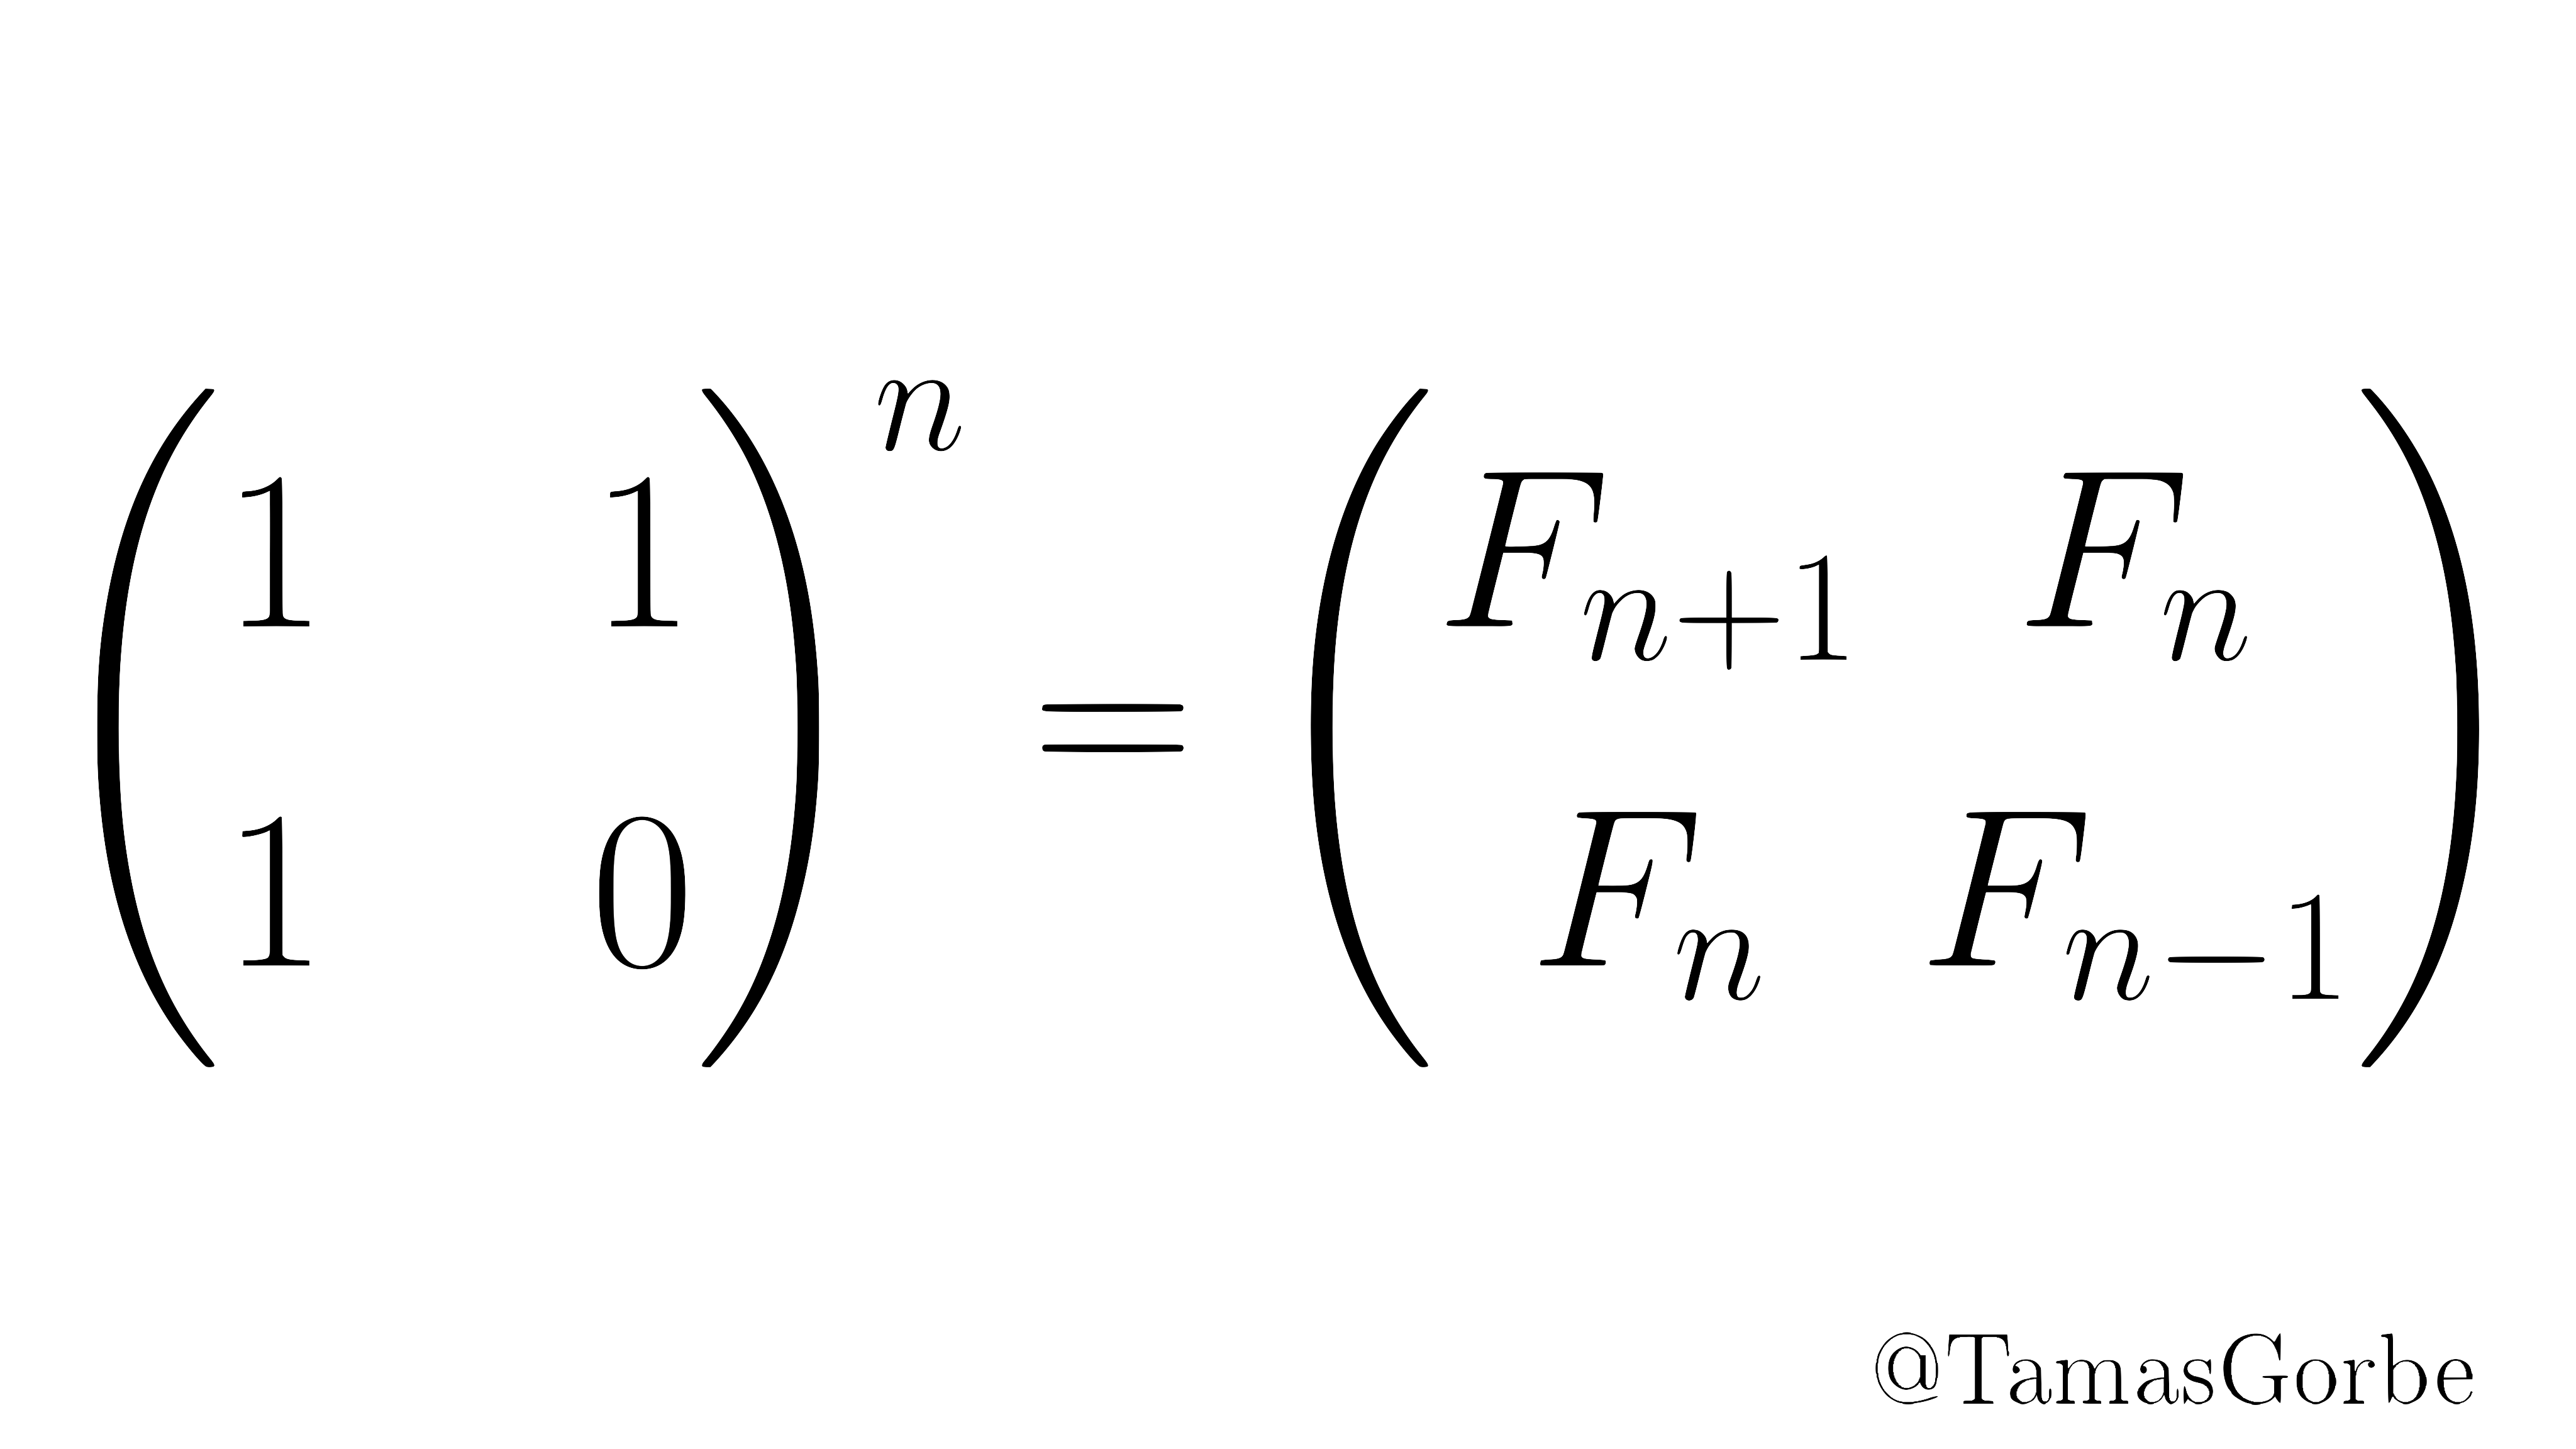
\includegraphics[width=1\textwidth]{imagenes/imagenes03/T03IM03.png}
\end{figure}

\end{myexampleblock}


\subsection{Cuestiones}

\begin{enumerate}[Q. 1] 

\item Sea $A_{m \times n}$

a) ¿Existe una matriz $B$ tal que $BA$ sea una matriz fila?, ¿cuál es su dimensión?

b) ¿Existe una matrz $B$ tal que $AB$ sea una matriz fila?, ¿cuál es su dimensión?

c) Si $AB$ es una matriz cuadrada, ¿qué dimensión tiene la matriz $B^TA^T$?

\rotatebox{180}{\leftline{\textcolor{gris}{\scriptsize{\hspace{5mm}  Ayuda: haz un análisis dimensional en cada caso. }}}}.

\item Considera las matrices $A_{m \times n}\; ; \; \; B_{p \times q}\;$. ¿Qué relación debe haber enre $m,n,p,q$ para que exista:?

a) $(AB)^{-1}$; \hspace{5mm} b) $A^2-B^2$; \hspace{5mm} c) $AB^T-A$

\rotatebox{180}{\leftline{\textcolor{gris}{\scriptsize{\hspace{5mm}  Ayuda: haz un análisis dimensional. }}}}.

\item Sean $A, B$ y $C$ tres matrices tales que $ABC$ es una matriz  $3 \times 2$ y $AC^T$ es una matriz cuadrada. Encuentra las dimensiones de $A$, $B$ y $C$.

\rotatebox{180}{\leftline{\textcolor{gris}{\scriptsize{\hspace{5mm}  Ayuda: haz un análisis dimensional. }}}}.

\item Si con las matrices $A,B,C$ y $D$ se pueden hacer las operaciones $(A+D)C^T; \; CBT; \text{ y }B^2$, ¿cuál de las operaciones siguientes se pede hacer:?

a) $\; CBD)^T\quad$ b) $\; C(D+A)B\quad$ c) $\; (BA^TD)^2\quad $ d) $\; (A^t+D^T)^2C$

\rotatebox{180}{\leftline{\textcolor{gris}{\scriptsize{\hspace{5mm}  Ayuda: solo el apartado c). }}}}.

\item  ?`Qué efecto tiene multiplicar una matriz diagonal de orden $3$, $\; D=Diag(\alpha,\beta,\gamma)=\left( \begin{array}{ccc} \alpha&0&0 \\0&\beta&0 \\ 0&0&\gamma \end{array} \right)\;$ por una matriz cuadrada $A$ cualquiera?

\rotatebox{180}{\leftline{\textcolor{gris}{\scriptsize{\hspace{5mm}  Ayuda: $AD=(\; \alpha c_1(A), \beta c_2(A), \gamma c_3(A) \;)\; \quad (DA)^T=(\; \alpha f_1(A), \beta f_2(A), \gamma f_3(A)\: ))$ }}}}.

\item Demuestra que si $A\in \mathcal M_{2 \times 2} \to (A^T)^2=(A^2)^T$

\rotatebox{180}{\leftline{\textcolor{gris}{\scriptsize{\hspace{5mm}  Ayuda: \scriptsize{$A=\left( \begin{matrix} a&b\\c&d \end{matrix} \right)$ y efectua las operaciones.} }}}}.

\item Encuentra las matrices $X$ que conmutan con $A=\left( \begin{matrix} 1&1\\1&1 \end{matrix} \right)$

\rotatebox{180}{\leftline{\textcolor{gris}{\scriptsize{\hspace{5mm}  Ayuda: $X=\left( \begin{matrix} a&b\\c&d \end{matrix} \right) \to AX=XA \Rightarrow X=\left( \begin{matrix} a&b\\b&a \end{matrix} \right)$ }}}}.

\item Encuentra las matrices $X$ que conmutan con $A=\left( \begin{matrix} 1&1\\0&1 \end{matrix} \right)$

\rotatebox{180}{\leftline{\textcolor{gris}{\scriptsize{\hspace{5mm}  Ayuda: $X=\left( \begin{matrix} a&b\\c&d \end{matrix} \right) \to AX=XA \Rightarrow X=\left( \begin{matrix} a&b\\0&a \end{matrix} \right)$ }}}}.

\item (*) Encuentra las matrices $X$ de segundo orden tales que $X^2=X$

\rotatebox{180}{\leftline{\textcolor{gris}{\scriptsize{\hspace{5mm}  Ayuda: $X:\; 
\left( \begin{matrix} 0&0\\0&0  \end{matrix} \right); \; 
\left( \begin{matrix} 1&0\\0&1  \end{matrix} \right); \; 
\left( \begin{matrix} a& \sqrt{a-a^2}\\ \sqrt{a-a^2}&1-a  \end{matrix} \right); \; 
 \left( \begin{matrix} a&\-sqrt{a-a^2}\\-\sqrt{a-a^2}&1-a  \end{matrix} \right) $ }}}}.

\item Demuestra que las matrices $M=\left( \begin{matrix} x&y\\y&x  \end{matrix}\right)$ e $N=\left( \begin{matrix} u&v\\v&u  \end{matrix}\right)$, conmutan.

\rotatebox{180}{\leftline{\textcolor{gris}{\scriptsize{\hspace{5mm}  Ayuda: $AB=BA$}}}}.

\item Prueba que $\forall A\in \mathcal M_{n \times n}$ se cumple que $A\cdot A^T$ es simetrica.

\rotatebox{180}{\leftline{\textcolor{gris}{\scriptsize{\hspace{5mm}  Ayuda: Calcula $(AA^T)^T$ y usa propiedades de la trasposición. (lema \ref{producto-traspuestas}) }}}}.

\item $M_{m \times n} \to MM^T \text { y } M^TM\; $ son, ambas, matrices simétricas.

\rotatebox{180}{\leftline{\textcolor{gris}{\scriptsize{\hspace{5mm}  Ayuda: $S$ simétrica si $S^T=T$ y usa propiedades de la trasposición. (lema \ref{producto-traspuestas}) }}}}.  

\item Prueba que si $A$ es idempotente, $A^2=A$, entonces, si  $B=2A-I$, se cumple que $B^2=I$

\rotatebox{180}{\leftline{\textcolor{gris}{\scriptsize{\hspace{5mm}  Ayuda: $B^2=B\cdot B=(2A-I)\cdot (2A-I)= \cdots$ }}}}.

\item (**) Encuentra todas las matrices ortogonales de orden 2, es decir, matrices $M$ tales que $MM^T=I \;\; (\;M^{-1}=M^T \;)$

\rotatebox{180}{\leftline{\textcolor{gris}{\scriptsize{\hspace{5mm}  Ayuda: $M=\left( \begin{matrix} a&b\\c&d   \end{matrix} \right) \to  
\left( \begin{matrix} \cos \theta & \sin \theta \\ -\sin \theta & \cos \theta   \end{matrix} \right) ; \; 
\left( \begin{matrix}  \cos \phi & \sin \phi \\ \sin \phi & - \cos \phi  \end{matrix} \right) ; \; \forall \theta,\phi \in \mathbb R$}}}}.

\item Sea $A$ una matriz cuadrada de orden $n$ tal que $A^2=0$:

a) Comprueba que $(A+I)^2=2A+I$

b) $B=I-A \; ; \quad C=A+I\;$. Comprueba que una es inversa de la otra.

\rotatebox{180}{\leftline{\textcolor{gris}{\scriptsize{\hspace{5mm}  Ayuda: a) $0$ es la matriz nula; $\quad$ b) calcula $BC$ }}}}.

\item Considera matrices triangulares cualquiera de orden 3 y comprueba que la suma, el producto por un número y el producto de matrices triangulares es triangular.

\rotatebox{180}{\leftline{\textcolor{gris}{\scriptsize{\hspace{5mm}  Ayuda: $A=\left( \begin{matrix} a&b&c\\0&d&e\\0&0&f  \end{matrix} \right); quad B=\left( \begin{matrix} x&y&z\\0&p&q\\0&0&r  \end{matrix} \right)  \to A+B; \; kA; \; AB$   }}}}.

\item Si la matriz $A$, de orden $n$, es invertible, entonces, la matriz $3A$:

\begin{multicols}{2}
\hspace{-11mm} \small{a) Es invertible y su inversa vale $3A^{-1}$}

\hspace{-11mm} \small{b) Es invertible y su inversa vale $3^n A^{-1}$}

\hspace{-6mm} \small{c) Es invertible y su inversa vale $\frac 1 3 A^{-1}$}

\hspace{-5mm}\small{d) No necesariamente es invertible.}
\end{multicols}

\rotatebox{180}{\leftline{\textcolor{gris}{\scriptsize{\hspace{5mm}  Ayuda: La respuesta correcta es la c) }}}}.

%\item

%\rotatebox{180}{\leftline{\textcolor{gris}{\scriptsize{\hspace{5mm}  Ayuda: }}}}.

%\item

%\rotatebox{180}{\leftline{\textcolor{gris}{\scriptsize{\hspace{5mm}  Ayuda: }}}}.

	
\end{enumerate}

\clearpage

\section{Resumen}

\begin{myalertblock}{Resumen de matrices}

$A=\left[
\begin{matrix}
a_{11} & a_{12} & \cdots & a_{1j} & \cdots & a_{1n} \\
a_{21} & a_{22} & \cdots & a_{2j} & \cdots & a_{2n} \\
a_{31} & a_{32} & \cdots & a_{3j} & \cdots & a_{3n} \\
\vdots & \vdots & \ddots & \vdots & \ddots & \vdots \\
a_{i1} & a_{i2} & \cdots & \boxed{a_{ij}} & \cdots & a_{in} \\
\vdots & \vdots & \ddots & \vdots & \ddots & \vdots \\
a_{m1} & a_{m2} & \cdots & a_{mj} & \cdots & a_{mn} \\
\end{matrix}
\right]$
\footnotesize{$= [a_{ij}]_{m \times n} \; \begin{cases}0\le i \le m; \\ 0\le j \le n\end{cases}$}

\vspace{3mm}
\centerline{$\boxed{\; \boldsymbol{A_{\;  (num. \; filas)\; \times \; (num. \; columnas) }}\; }$}

\vspace{2mm} Traspuesta: $\quad (a_{ij})^T=(a_{ji})$

\vspace{2mm} Producto por un número real: $\quad k(a_{ij})=(ka_{ij})$

\vspace{2mm} Suma: $\quad (a_{ij})_{m \times n}\; + \; (b_{ij})_{m \times n}=(a_{ij}+b_{ij})_{m \times n}$

\hspace{12mm} asociaiva, conmutativa, neutro $\boldsymbol{0}$, opuesto $-A$

\vspace{2mm} Producto: $\quad (a_{il})_{m \times \cancel{n}} \; \cdot \;(b_{lj})_{\cancel{n} \times p} \; = \; (f_i(A)\cdot c_j(B))_{m \times p}$

\hspace{15mm} \scriptsize{$AB \neq BA$, asociativa, distributivas, neutro $IA=AI=A$, inversa $A^{1}$}\footnotesize{.}

\hspace{12mm} $\quad A \in \mathcal M_n: \quad \exists A^{-1}\; / \; AA^{-1}=A^{-1}A=I$

\vspace{2mm} Potencias:  $\quad M\in \mathcal M_n :\quad M^n$

\vspace{2mm} Propiedades: $(A+B)^T=A^T+B^T \quad $ $(AB)^T=B^TA^T \quad $ $(AB)^{-1}=B^{-1}A^{-1} \quad $ $(A^{-1})^{-1}=A \quad $ $(A^T)^{-1}=(A^{-1})^T$

\vspace{2mm} Inversa por Gaus: $ \quad [\; A \; | \; I \; ] \; \to \text{ transf. Gauss } \to  \; [\; I \; | \; \boldsymbol{ A^{-1} } \; ] $\normalsize{.}

\end{myalertblock}


%$A=\left( \begin{matrix}   \end{matrix}\right)$

	%\begin{figure}[H]
		%\centering
		%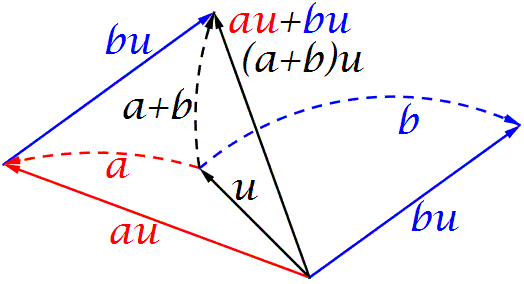
\includegraphics[width=0.5\textwidth]{imagenes/imagenes01/T01IM01.png}
		%\caption{Los dos problemas clásicos del cálculo: trazado de tangentes y áreas bajo curvas.}
	%\end{figure}
		
%varios párrafos encuadrados - explicaciones ad hoc
%\centering{
%\fbox{
%\parbox{0.95\textwidth}{
%varios
%
%$parrafos
%
%dentro
%}
%}
%}
% \justify


%\rotatebox{180}{\leftline{\textcolor{gris}{tararí}}}.

\chapter{Determinantes}	

\section{Determinantes ordenes 1 , 2 y 3}

\begin{defi}
El `determinante' es una aplicación que, para cada matriz cuadrada $A$ de orden $n$ le hace corresponder un número real que se denota por $det(A)$ o $|A|$:

\vspace{2mm}\centerline{\colorbox{LightYellow}{$\boxed{\; A\in \mathcal M_n \to det(A)=|A|\in \mathbb R\; }$}}

\vspace{3mm} --- Determinantes orden $1$: $A=[a_{11}] \to det(A)=|A|=|a_{11}|=a_{11}$

¡Cuidado! : No confundir $det(a_{11})=|a_{11}|$ con el valor absoluto $|a_{11}|$. De todos modos, los determinantes de orden uno no se suelen usar.

\vspace{3mm} --- Determinantes orden $2$: $A=\left[
\begin{array}{cc}
a_{11} & a_{12} \\
a_{21} & a_{22}
\end{array}
\right]	
 \to det(A)=|A|=\left|
 \begin{array}{cc}
a_{11} & a_{12} \\
a_{21} & a_{22}
\end{array} \right|=$
$=\begin{array}{cc}
\textcolor{blue}{a_{11}} & a_{12} \\
a_{21} & \textcolor{blue}{a_{22}}
\end{array} \; -\; 
\begin{array}{cc}
a_{11} & \textcolor{red}{a_{12}} \\
\textcolor{red}{a_{21}} & a_{22}
\end{array}
=\textcolor{blue}{a_{11}a_{22}} - \textcolor{red}{a_{12}a_{21}}$




\vspace{3mm} --- Determinantes orden $3$: `Regla de Sarrus'

$A=\left[ \begin{array}{ccc}
a_{11} & a_{12} & a_{13} \\
a_{21} & a_{22} & a_{23} \\
a_{31} & a_{32} & a_{33}
\end{array}   \right] \to det(A)=|A|=$

$=\left|
\begin{array}{ccc}
a_{11} & a_{12} & a_{13} \\
a_{21} & a_{22} & a_{23} \\
a_{31} & a_{32} & a_{33}
\end{array}
\right|= \; 
\begin{array}{ccc}
\textcolor{blue}{a_{11}} & \textcolor{DarkGreen}{a_{12}} & \textcolor{red}{a_{13}} \\
\textcolor{red}{a_{21}} & \textcolor{blue}{a_{22}} & \textcolor{DarkGreen}{a_{23}} \\
\textcolor{DarkGreen}{a_{31}} & \textcolor{red}{a_{32}} & \textcolor{blue}{a_{33}}
\end{array} 
\; - \;  
\begin{array}{ccc}
\textcolor{red}{a_{11}} & \textcolor{DarkGreen}{a_{12}} & \textcolor{blue}{a_{13}} \\
\textcolor{DarkGreen}{a_{21}} & \textcolor{blue}{a_{22}} & \textcolor{red}{a_{23}} \\
\textcolor{blue}{a_{31}} & \textcolor{red}{a_{32}} & \textcolor{DarkGreen}{a_{33}}
\end{array}
 =$

$\quad$

\noindent $= \textcolor{blue}{a_{11}a_{22}a_{33}} + \textcolor{red}{a_{21}a_{32}a_{13}} + \textcolor{DarkGreen}{a_{31}a_{23}a_{12}} \; - \; (\textcolor{blue}{a_{13}a_{22}a_{31}} + \textcolor{red}{a_{23}a_{32}a_{11}} + \textcolor{DarkGreen}{a_{33}a_{21}a_{12})}$

\end{defi}

\begin{figure}[H]
	\centering
	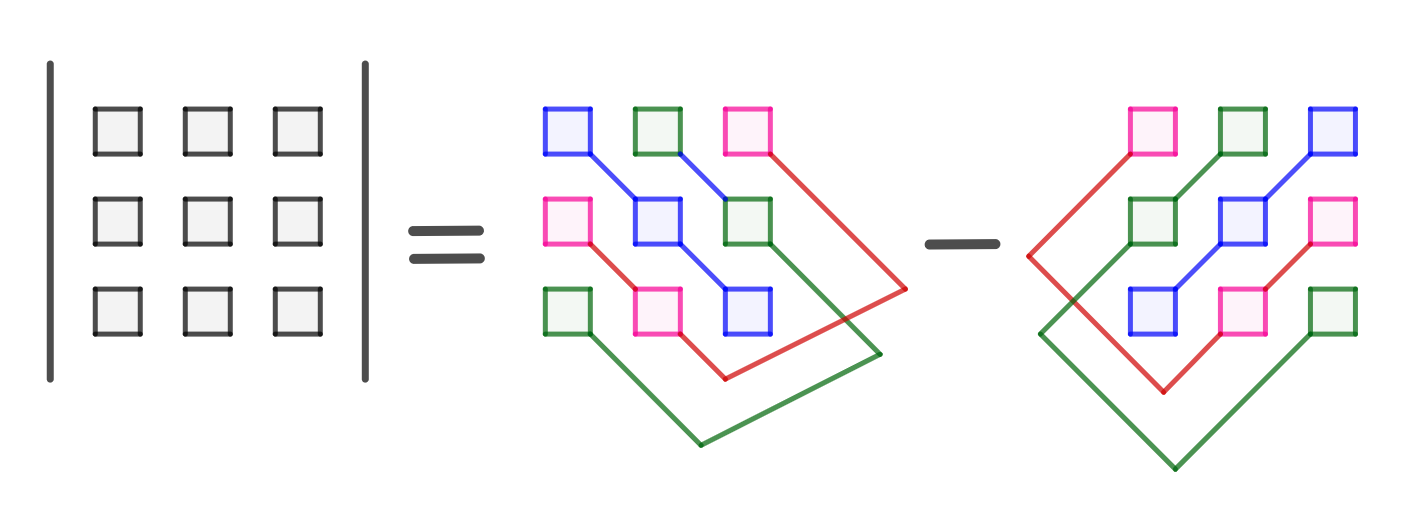
\includegraphics[width=1\textwidth]{imagenes/imagenes04/T04IM03.png}
\end{figure}

\rule{30mm}{0.1mm}

Otra regla para recordar la regla de Sarrus consiste en repetir, al final del determinante las filas $1$ y $2$ y multiplicar los elementos de las diagonales (izquierda a derecha positivas, derecha a izquierda negativas).

$|A|=\left |
\begin{array}{ccc}
a_{11} & a_{12} & a_{13} \\
a_{21} & a_{22} & a_{23} \\
a_{31} & a_{32} & a_{33}
\end{array}
\right|=
\begin{array}{ccc}
\textcolor{blue}{a_{11}} & a_{12} & a_{13} \\
\textcolor{red}{a_{21}} & \textcolor{blue}{a_{22}} & a_{23} \\
\textcolor{DarkGreen}{a_{31}} & \textcolor{red}{a_{32}} & \textcolor{blue}{a_{33}} \\
a_{11} & \textcolor{DarkGreen}{a_{12}} & \textcolor{red}{a_{13}} \\
a_{21} & a_{22} & \textcolor{DarkGreen}{a_{23}} \\
\end{array} \; - \; 
\begin{array}{ccc}
a_{11} & a_{12} & \textcolor{blue}{a_{13}} \\
a_{21} & \textcolor{blue}{a_{22}} & \textcolor{red}{a_{23}} \\
\textcolor{blue}{a_{31}} & \textcolor{red}{a_{32}} & \textcolor{DarkGreen}{a_{33}} \\
\textcolor{red}{a_{11}} & \textcolor{DarkGreen}{a_{12}} & a_{13} \\
\textcolor{DarkGreen}{a_{21}} & a_{22} & a_{23} \\
\end{array} =$

\noindent $\textcolor{blue}{a_{11}a_{22}a_{33}} + \textcolor{red}{a_{21}a_{32}a_{13}} + \textcolor{DarkGreen}{a_{31}a_{23}a_{12}} \; - \; (\textcolor{blue}{a_{13}a_{22}a_{31}} + \textcolor{red}{a_{23}a_{32}a_{11}} + \textcolor{DarkGreen}{a_{33}a_{21}a_{12})}$

Aunque es recomendable recordar la técnica anterior (mayor rapidez de cálculo mental).

\rule{30mm}{0.1mm}

\begin{ejem}
Calcula los determinantes de: 

$A=[-7/4]; \; B=\left[ \begin{array}{cc} 3&-2\\5&2  \end{array} \right]; \;  C=\left[ \begin{array}{ccc}  1 &2  &3 \\ -3&0&4 \\ 2&-1&3  \end{array} \right]$

\noindent $|A|=-7/4$

\noindent $|B|=3\cdot 2 - ((-2)\cdot 5)=6+10=16$

\noindent $|C|=1\cdot 0\cdot 3 + (-3)\cdot (-1)\cdot 3+ 2\cdot 4 \cdot 2 -(3\cdot 0 \cdot 2 + 4\cdot (-1)\cdot 1 + 3\cdot (-3)\cdot 2)=
0+9+16-(0-4-18)=25+22=47$
\end{ejem}

Para orden $4$ o superior, se recurre al desarrollo de Laplace para el cálculo de determinantes (no es válida la regla de Sarrus). Se verá en próximos apartados.

Obsérvese que para las matrices usamos paréntesis o corchetes $(a_{ij}) \text{ ó } [a_{ij}]\; $ y para los determinantes barras $|a_{ij}|$.

\section{Propiedades de los determinantes}.

Las propiedades que vamos a enunciar son válidas para determinantes de cualquier orden. Las demostraciones sobrepasan, con mucho, los objetivos de un curso de bachillerato; por lo que para cada una de ellas nos contentaremos con una mera comprobación con determinantes de ordenes $2$ o $3$, que son los que de momento, conocemos.

\begin{enumerate}[P.D. 1]
\item \colorbox{LightYellow}{$\boxed{\; |A|=|A^T|\; }$}. El determinante de una matriz coincide con el de su traspuesta.

\underline{Comprobación:}  $|A|=\left | \begin{array}{cc} 3&-2\\5&4  \end{array} \right| = 12-(-10)=22$

$|A^T|=\left | \begin{array}{cc} 3&5\\-2&4  \end{array} \right| = 12-(-10)=22$

¡ A partir de esta propiedad, todo lo que se diga para `filas' valdrá para `columnas' y viceversa !

\item Si un determinante contiene \colorbox{LightYellow}{una fila (o columna) de ceros}, el determinante es cero

\underline{Comprobación:} $|M|=\left| \begin{array}{ccc} 1&2&3\\0&0&0\\-2&3&5 \end{array} \right|= 0+0+0-(0+0+0)=0$

¡Para abreviar, en adelante, nos referiremos a `líneas' de un determinante queriendo indicar filas o columnas!

En general:

 $Det(c_1, c_2, \cdots, \textcolor{blue}{0}, \cdots , c_n)=0$, ó  $Det(f_1, f_2, \cdots, \textcolor{red}{0}, \cdots , f_n)=\textcolor{DarkGreen}{0}$
 
 Donde, con $c_1, c_2, \cdots, c_n$ queremos indicar las columnas de $M$, así como con $f_1,f_2, \cdots , f_n$ sus filas.

\item Si se \colorbox{LightYellow}{intercambian de posición dos líneas} de un determinante (dos filas o dos columnas), el determinante cambia de signo.

\underline{Comprobación:}  $\left| \begin{array}{ccc} \textcolor{blue}{1}& \textcolor{blue}{2}& \textcolor{blue}{3}\\-2&0&3\\ \textcolor{red}{-2}& \textcolor{red}{3}& \textcolor{red}{5} \end{array} \right|= 
0-18-12-(0+9-20)=-30-(-11)=-19$

 $\left| \begin{array}{ccc} \textcolor{red}{-2}& \textcolor{red}{3}& \textcolor{red}{5} \\-2&0&3\\ \textcolor{blue}{1}& \textcolor{blue}{2}& \textcolor{blue}{3}  \end{array} \right|= 
0-20+9-(0-12-18)=-11-(-30)=19$

En general: 

$Det(f_1, \cdots , \textcolor{blue}{f_i}, \cdots , \textcolor{red}{f_j} \cdots , f_n)=\textcolor{DarkGreen}- Det(f_1, \cdots , \textcolor{red}{f_j}, \cdots , \textcolor{blue}{f_i} \cdots , f_n)$

ó 

$Det(c_1, \cdots , \textcolor{blue}{c_i}, \cdots , \textcolor{red}{c_j} \cdots , c_n)=\textcolor{DarkGreen}{-} Det(c_1, \cdots , \textcolor{red}{c_j}, \cdots , \textcolor{blue}{c_i} \cdots , c_n)$

\item A una línea (fila o columna) de un determinante, si se le \colorbox{LightYellow}{añade otra} \colorbox{LightYellow}{línea} (fila o columna) del mismo determinante multiplicada por un número, el determinante no varía.

En general:

\small{$Det(f_1, \cdots , \textcolor{blue}{f_i},\cdots , f_j,  \cdots , f_n)= Det(f_1, \cdots , \textcolor{blue}{f_i}+ \textcolor{DarkGreen}{k}\cdot  \textcolor{red}{f_j}, \cdots, f_j,  \cdots , f_n)$} 

\normalsize{ó} 

\small{$Det(c_1, \cdots , \textcolor{blue}{c_i},\cdots , c_j,  \cdots , c_n)= Det(c_1, \cdots , \textcolor{blue}{c_i}+ \textcolor{DarkGreen}{k}\cdot  \textcolor{red}{c_j}, \cdots, c_j,  \cdots , c_n)$} 

\normalsize{\underline{Comprobación:}} $\left| \begin{array}{cc} 1&2\\3&4 \end{array} \right|=4-6=-2 \quad \textcolor{gris}{[\; F2 \to F2+5F1 \Rightarrow\; ]}$

$\left| \begin{array}{cc} \textcolor{blue}{1}&\textcolor{blue}{2}\\3+\textcolor{red}{5}\cdot \textcolor{blue}{1}&4+\textcolor{red}{5}\cdot \textcolor{blue}{2} \end{array} \right|=\left| \begin{array}{cc} 1&2\\8&14 \end{array} \right|=14-16=-2$

\item Si en un determinante hay una \colorbox{LightYellow}{línea igual o proporcional} a otra, el determinante es cero.

$Det(f_1, \cdots , \textcolor{blue}{f_i}, \cdots , \textcolor{red}{k} \cdot \textcolor{blue}{f_i}, \cdots , f_n)=0$

ó 

$Det(c_1, \cdots , \textcolor{blue}{c_i}, \cdots , \textcolor{red}{k}\cdot \textcolor{blue}{c_i}, \cdots , c_n)=0$

\underline{Comprobación:} 
$\; \left| \begin{array}{ccc} 1&-2&5\\-3&6&0 \\4&-8&-1 \end{array} \right|= 
-6+120+0-(120+0-6)=
\left| \begin{array}{ccc} \textcolor{blue}{1}&\textcolor{red}{-2}\cdot \textcolor{blue}{1}&5\\\textcolor{blue}{-3}&\textcolor{red}{-2} \cdot \textcolor{blue}{(-3)}&0 \\\textcolor{blue}{4}&\textcolor{red}{-2} \cdot \textcolor{blue}{4}&-1 \end{array} \right|=0$, ya que $c2=2c1$	


\item Producto de un \colorbox{LightYellow}{número por un determinante} o \colorbox{LightYellow}{`factor común'}:

$\textcolor{blue}{k}\cdot Det(f_1, \cdots , f_i, \cdots, f_j, \cdots , f_n)=
Det(f_1, \cdots , \textcolor{red}{k}\cdot f_i, \cdots, f_j, \cdots , f_n) =
Det(f_1, \cdots , f_i, \cdots, \textcolor{red}{k} \cdot f_j, \cdots , f_n)=
Det(\textcolor{red}{k} \cdot f_1, \cdots , f_i, \cdots, f_j, \cdots , f_n)= \cdots$

ó 

$\textcolor{blue}{k}\cdot Det(c_1, \cdots , c_i, \cdots, c_j, \cdots , c_n)=
Det(c_1, \cdots , \textcolor{red}{k}\cdot c_i, \cdots, c_j, \cdots , c_n) =
Det(c_1, \cdots , c_i, \cdots, \textcolor{red}{k} \cdot c_j, \cdots , c_n)=
Det(\cdot c_1, \cdots , c_i, \cdots, c_j, \cdots , \textcolor{red}{k} c_n)= \cdots$

Esta propiedad, leída de derecha a izquierda, es la '`propiedad de factor común para determinantes': si en un determinante hay una línea (fila o columna) multiplicada por un número, éste puede salir fuera del determinante multiplicando.

\underline{Comprobación:} $\textcolor{blue}{5}\cdot \left| \begin{array}{cc} 1&2\\3&4 \end{array} \right|=5\cdot (4-6)=\textcolor{blue}{5}\cdot (-2)=-10$

$\left| \begin{array}{cc} \textcolor{blue}{5}\cdot 1&\textcolor{blue}{5}\cdot 2\\3&4 \end{array} \right|=\left| \begin{array}{cc} 5&10\\3&4 \end{array} \right|=20-30=-10$

$\left| \begin{array}{cc} 1&\textcolor{blue}{5}\cdot 2\\3&\textcolor{blue}{5} \cdot 4 \end{array} \right|=\left| \begin{array}{cc} 1&10\\3&20 \end{array} \right|=20-30=-10$  

Vista como factor común: $ \left| \begin{array}{cc} 10&2\\60&8 \end{array} \right|=80-120=-40$, pero 

$ \left| \begin{array}{cc} 10&2\\60&8 \end{array} \right| =  \left| \begin{array}{cc} \textcolor{blue}{10}\cdot 1&2\\\textcolor{blue}{10} \cdot 6&8 \end{array} \right|  = \textcolor{blue}{10} \cdot  \left| \begin{array}{cc} 1&2\\6&8 \end{array} \right| = 
\textcolor{blue}{10} \cdot  \left| \begin{array}{cc} 1&2\\\textcolor{red}{2}\cdot 3&\textcolor{red}{2} \cdot 4 \end{array} \right|= \textcolor{blue}{10}\cdot \textcolor{red}{2} \cdot  \left| \begin{array}{cc} 1&2\\3&4 \end{array} \right|= \textcolor{blue}{10}\cdot \textcolor{red}{2} \cdot (4-6)=10\cdot 2\cdot (-2)=-40$

IMPORTANTE: Si $A$ es una matriz cuadrada de orden $n$ (n-filas y n-columnas), como $k\cdot A$ consiste en multiplicar por $k$ TODAS las filas (columnas) de $A$, para calcular su determinante, podemos sacar $n$-veces el número $k$ factor común de cada una de sus filas (columnas), por lo que:

\vspace{2mm} \centerline{\colorbox{LightYellow}{$\boxed{\;k\in \mathcal M_n \to det(k\cdot A)= k^n\cdot |A|\; }$}}

Nótese la diferencia de $k[A]$ y $k|A|$, el primer producto es el de un número por una matriz y el número multiplica a todos los elementos de la matriz, en el segundo caso tenemos el producto de un número por un determinante y solo se multiplica el número por una sola de sus líneas (filas o columnas).

\item Se pueden \colorbox{LightYellow}{sumar dos determinantes} de matrices del mismo tipo si las matrices son en todos sus elementos iguales excepto en una de sus líneas (fila o columna), siendo ésta la que se suma. Vista la propiedad al revés, permite descomponer un determinante como suma de otros dos en todo iguales excepto en una de sus líneas.

Generalización a determinantes de orden 3:

$\left| \begin{array}{ccc} a&b&c \\ \textcolor{blue}{x_1}&\textcolor{blue}{y_1}&\textcolor{blue}{z_1} \\ u&v&w \end{array} \right| +  
\left| \begin{array}{ccc} a&b&c \\ \textcolor{red}{x_2}&\textcolor{red}{y_2}&\textcolor{red}{z_2} \\ u&v&w \end{array} \right| =
\left| \begin{array}{ccc} a&b&c \\ \textcolor{blue}{x_1}+\textcolor{red}{x_2}&\textcolor{blue}{y_1}+\textcolor{red}{y_2}&\textcolor{blue}{z_1}+\textcolor{red}{z_2} \\ u&v&w \end{array} \right|$

\underline{Comprobación:} $\; \left| \begin{array}{cc} \textcolor{red}{4}+ \textcolor{blue}{2} \;\textcolor{gris}{(=6)}&7\\ \textcolor{red}{-3}+ \textcolor{blue}{5} \;\textcolor{gris}{(=2)}&2 \end{array} \right| =
\left| \begin{array}{cc} \textcolor{red}{4}&7\\ \textcolor{red}{-3}&2 \end{array} \right|+
\left| \begin{array}{cc} \textcolor{blue}{2} &7\\ \textcolor{blue}{5} &2 \end{array} \right|
 =$
 
 $= 12-14 = \boldsymbol{-2}= 8-(-21) \; + \; 4-(35)=29\; - \; 31 =\boldsymbol{-2} $
 
 \item El \colorbox{LightYellow}{determinante de una matriz triangular} es el producto de los elementos de la diagonal principal.
 
 En general: $\displaystyle \left| \begin{array}{cccc} a_{11} & a_{2n} & \cdots  &a_{2n}  \\ 0&a_{22}&\cdots&a_{2n}        \\0&\vdots & \ddots & \vdots \\ 0 & 0& \cdots & a_{nn} \end{array} \right| =
 a_{11} \cdot a_{22} \cdots a_{nn}=\prod_{i=1}^n a_{ii}$
 
 \underline{Comprobación:} $\left| \begin{array}{ccc}
 \textcolor{blue}{5}&\textcolor{red}0&\textcolor{red}0\\ -3&\textcolor{blue}{2}&\textcolor{red}0 \\4&-3&\textcolor{blue}{2} \end{array} \right|= \textcolor{blue}{5} \cdot \textcolor{blue}{2} \cdot \textcolor{blue}{2} +0+0-(0+0+0)=20$	
 
 \emph{Consecuencia:} \colorbox{LightYellow}{$\; \boxed {\; |I|=1\; }$}
 
 \item El determinante del producto es igual al producto de los determinantes:
 $\quad$\colorbox{LightYellow}{$\; \boxed {\; |A\cdot B|= |A| \cdot |B| \; }$}

\underline{Comprobación:} $A=\left[ \begin{array}{cc} 1&2\\3&4 \end{array} \right]; \quad B=\left[ \begin{array}{cc} 1&-1\\0&2 \end{array} \right] \to$

\noindent --- $A\cdot B= \left[ \begin{array}{cc} 1&3\\3&5 \end{array} \right] \to det(A\cdot B)= 5-9=\boldsymbol{-4}$

\noindent --- $det(A)=4-6=-2; \; det(B)=2-0=2 \to det(A) \cdot det(B)=(-2)\cdot 2=\boldsymbol{-4}$  

\item Como corolarios a la propiedad anterior: `el determinante de la potencia es la potencia del determinante' y `el determinante de la inversa es la inversa del determinante':

Como $A^n=A\cdot A \cdot \underset{\text{n-veces}}{\cdots} \cdot A $ y la propiedad anterior, deducimos que:

\vspace{2mm} \centerline{\colorbox{LightYellow}{$\; \boxed {\; |A^{n}|= |A|^n \; }$}}

 De $A\cdot A^{-1}=I; \quad |I|=1$ y la propiedad anterior, deducimos que:

\vspace{2mm} \centerline{\colorbox{LightYellow}{$\; \boxed {\; |A^{-1}|= \dfrac {1}{|A|} \; }$}}

\end{enumerate}

\normalsize{En ejercicios se verán aplicaciones las propiedades de los determinantes.}



\begin{myexampleblock}{La historia de los determinantes}

\small{Los determinantes hicieron su aparición en las matemáticas más de un siglo antes que las matrices. El término matriz fue creado por James Joseph Sylvester.}

\small{\vspace{1mm} Algunos de los más grandes matemáticos de los siglos XVIII y XIX contribuyeron al desarrollo de las propiedades de los determinantes. La mayoría de los historiadores coinciden en afirmar que la teoría de los determinantes se originó con el matemático alemán Gottfried Wilhelm Leibniz (1646-1716). Leibniz empleó los determinantes en 1693 con relación a los sistemas de ecuaciones lineales simultáneas. No obstante hay quienes creen que el matemático japonés Seki Kowa hizo lo mismo unos años antes.}

\small{\vspace{1mm} Las contribuciones más prolíficas a la teoría de los determinantes fueron las del matemático francés Agustin-Louis Cauchy (1789-1857). Cauchy escribió, en 1812 una memoria de 84 páginas que contenía la primera demostración de la fórmula $\; |A\cdot B|=|A|\cdot |B|$}

\small{\vspace{1mm} Hay algunos otros matemáticos que merecen ser mencionados aquí. El desarrollo de un determinante por cofactores fue empleado por primera vez por el matemático francés Pierre de Laplace (1749-1827).} 

\small{\vspace{1mm} Un contribuyente principal en la teoría de los determinantes fue el matemático alemán Carl Gustav Jacobi (1804-1851). Fue él con quien la palabra “determinante” ganó la aceptación definitiva.}

\rightline{\footnotesize{\emph{Fuente: Wikipedia}}\normalsize{.}}

\end{myexampleblock}



\justify


\section[Menor complementario y adjunto. Desarrollo de Laplace]{Menor complementario y adjunto. Desarrollo de Laplace}\sectionmark{Menores y adjuntos}
\sectionmark{Menores y adjuntos}


Para poder calcular determinantes de orden mayor que $3$ hemos de introducir los conceptos de `menor  complementario' y `adjunto' de un elemento de una matriz cuadrada.

\begin{defi}
Sea $A\in \mathcal M_{n\times n}$ una matriz cuadrada de orden $n$. Para cualquier elemento $a_{ij} \in A$ se define su `menor' correspondiente, y se representa por $M_{ij}$ al determinantes de orden $n-1$ que queda al eliminar de $A$ la fila$-i$ y la columna$-j$	.

Se llama `adjunto o cofactor' de $a_{ij}$ y se representa por $A_{ij}$ al menor $M_{ij}$ multiplicado por $1$ o $-1$ según sea la paridad de la suma de índices $i$ y $j$, es decir:

\centerline{\colorbox{LightYellow}{$\; \boxed{\; A_{ij}= (-1)^{i+j} \cdot M_{ij} \;}\;$}}

\end{defi}

\begin{ejem}
Sea $A=\left( \begin{matrix} 1&2&3\\4&5&6\\7&8&9 \end{matrix} \right)$. Calcula $M_{12};\; A_{12};\; M_{23};\; A_{23};\; M_{31};\; A_{31}$	

$M_{12}=\left| \begin{matrix} \cancel{1}& \boxed{\cancel{2}}&\cancel{3}\\4&\cancel{5}&6\\7&\cancel{8}&9 \end{matrix} \right|= 
\left| \begin{matrix} 4&6\\7&9 \end{matrix} \right|= 36-28=8\; $ \scriptsize{(tachamos fila 1 y columna 2)}\normalsize{.}

$A_{12}=(-1)^{1+2}\cdot M_{12}=(-1)^3\cdot 8=-8$

$M_{23}=\left| \begin{matrix} 1&2&\cancel{3}\\\cancel{4}&\cancel{5}&  \boxed{\cancel{6}} \\7&8&\cancel{9} \end{matrix} \right|=
  \left| \begin{matrix} 1&2\\7&8 \end{matrix} \right|=
  8-14=-6  $ \scriptsize{(tachamos fila 2 y columna 3)}\normalsize{.}
  
  $A_{23}=(-1)^{2+3}\cdot M_{2,3}=(-1)^5\cdot (-6)=6$
  
  $M_{31}=\left| \begin{matrix} \cancel{1}&2&3\\ \cancel{4}&5&6\\ \boxed{\cancel{7}} &\cancel{8}&\cancel{9} \end{matrix} \right|
   \left| \begin{matrix} 2&3\\5&6 \end{matrix} \right| = 12-15=-3  $
   
   $A_{31}=(-1)^{3+1}\cdot M_{31}=(-1)^4\cdot (-3)=-3$

\end{ejem}


\begin{defi}
Dada una matriz cuadrada $A$ se llama `matriz adjunta' a la que resulta de reemplazar en $A$ cada elemento $a_{ij}	$ por su correspondiente adjunto $A_{ij}$. Así, p.e., para una matriz de orden 3:

$A=\left[ \begin{matrix} a_{11}&a_{12}&a_{13}\\a_{21}&a_{22}&a_{23}\\a_{31}&a_{32}&a_{33} \end{matrix} \right] \Rightarrow  \; \; 
ad(A)=\left[ \begin{matrix} A_{11}&A_{12}&A_{13}\\A_{21}&A_{22}&A_{23}\\A_{31}&A_{32}&A_{33} \end{matrix} \right]$
\end{defi}

\begin{ejem} $A=\left[ \begin{matrix} 1&2&3 \\ 4&5&6 \\ 7&8&9 \end{matrix} \right]$, calcula su matriz adjunta.

$A_{11}=(-1)^{1+1}\; M_{11} =\left| \begin{matrix} 5&8\\8&9 \end{matrix} \right| = 45-64=-19$

$A_{12}=(-1)^{1+2}\; M_{12} =- \left| \begin{matrix} 4&6\\7&9 \end{matrix} \right| =- (36-42)=-(-6)=6$

$A_{13}=(-1)^{1+3}\; M_{13} =\left| \begin{matrix} 4&5\\7&8 \end{matrix} \right| = 32-35=-3$

$A_{21}=(-1)^{2+1}\; M_{21} =-\left| \begin{matrix} 2&3\\8&9 \end{matrix} \right| = -(18-24)=-(-6)=6$

$A_{22}=(-1)^{2+2}\; M_{22} =\left| \begin{matrix} 1&3\\7&9 \end{matrix} \right| = 9-21=-12$

$A_{23}=(-1)^{2+3}\; M_{23} =-\left| \begin{matrix} 1&2\\7&8 \end{matrix} \right| = -(8-14)=-(-6)=6$

$A_{31}=(-1)^{3+1}\; M_{31} =\left| \begin{matrix} 2&3\\5&6 \end{matrix} \right| = 12-15=-3$

$A_{32}=(-1)^{3+2}\; M_{32} =- \left| \begin{matrix} 1&3\\4&6 \end{matrix} \right| = -(6-12)=-(-6)=6$

$A_{33}=(-1)^{3+3}\; M_{33} =\left| \begin{matrix} 1&2\\4&5 \end{matrix} \right| = 5-8=-3$

Luego: $\; \; ad(A)=\left[ \begin{matrix} -19&6&-3\\6&-12&6\\-3&6&-3\end{matrix} \right]$

\end{ejem}


El siguiente teorema, que daremos sin demostración, permite calcular el determinante de cualquier matriz cuadrada de orden $n$ \textcolor{gris}{($\forall n \in \mathbb N$)} en función, eso sí, de $n$ determinantes de orden $n-1$. Se trata del `desarrollo de Laplace'.

\begin{teor}{Desarrollo de Laplace de un determinante.}
	
	El determinante de una matriz se puede desarrollar como suma de los productos de los elementos de una línea (fila o columna) cualquiera por sus correspondientes adjuntos.
	
	Sea $A=\left[
\begin{matrix}
a_{11} & a_{12} & \cdots & a_{1j} & \cdots & a_{1n} \\
a_{21} & a_{22} & \cdots & a_{2j} & \cdots & a_{2n} \\
a_{31} & a_{32} & \cdots & a_{3j} & \cdots & a_{3n} \\
\vdots & \vdots & \ddots & \vdots & \ddots & \vdots \\
a_{i1} & a_{i2} & \cdots & a_{ij} & \cdots & a_{in} \\
\vdots & \vdots & \ddots & \vdots & \ddots & \vdots \\
a_{m1} & a_{m2} & \cdots & a_{mj} & \cdots & a_{mn} \\
\end{matrix}
\right] \Rightarrow$

\vspace{3mm} $|A|=a_{11}A_{11}+a_{12}A_{12}+\cdots +a_{1n}A_{1n} \text{ (desarrollo primera fila) }= $

$=a_{13}A_{13}+a_{23}A_{23}+\cdots +a_{n3}A_{n3} \text{ (desarrollo tercera columna) } = $

$=a_{1j}A_{1j}+a_{2j}A_{2j}+\cdots +a_{nj}A_{nj} \text{ desarrollo columna-j )}= \displaystyle \sum_{k=1}^n a_{kj}A_{kj} =$

$=a_{i1}A_{i1}+a_{i2}A_{i2}+\cdots +a_{in}A_{in} \text{ (desarrollo fila-i) } = \displaystyle \sum_{k=1}^n a_{ik}A_{ik}=etc$
	
\end{teor}

\begin{ejem} Usando el desarrollo de Laplace:

Calcula: $a)\;  \left| \begin{matrix} 1&2&3\\4&5&6\\7&8&9 \end{matrix} \right|; \quad b)\; 
\left| \begin{matrix} 1&0&3&-1\\0&2&-1&-2\\2&0&5&2 \\ 0&0&-3&1  \end{matrix} \right|\quad c)\; \left| \begin{matrix} 1&5\\-3&3 \end{matrix} \right|$ 

----- Cálculo del $|A|$ :

* por adjuntos de la tercera columna:

$|A|= 
3\cdot (-1)^{3+1}\cdot \left| \begin{matrix} 4&5 \\ 7&8 \end{matrix} \right|	+
6\cdot (-1)^{3+2}\cdot \left| \begin{matrix} 1&2 \\ 7&8 \end{matrix} \right|+
9\cdot (-1)^{3+3}\cdot \left| \begin{matrix} 1&2 \\ 4&5 \end{matrix} \right|
=
3\cdot (+1) \cdot (32-35) + 6\cdot (-1) (8-14) + 9 \cdot (+1) \cdot (5-8)=
-9 +36 -27=0$

* por adjuntos de la segunda fila:

$|A|=4\cdot (-1)^{2+1}\left| \begin{matrix} 2&3\\8&9  \end{matrix} \right| +
5\cdot (-1)^{2+2}\cdot \left| \begin{matrix} 1&3\\7&9  \end{matrix} \right|+
6\cdot (-1)^{2+3}\cdot \left| \begin{matrix} 1&2\\7&8  \end{matrix} \right|=
 4\cdot (-1) \cdot (18-24) + 5\cdot (+1)\cdot (9-21) + 6 \cdot (-1) (8-14)=
 24-60+36 =0 $
 
 * por Sarrus, evidentemente, también dará cero:
 
 $A= 45+96+84-(105+48+72)=225-225=0$
 
 ----- Cálculo del $|B|$:
 
 * por adjuntos de la tercera fila:

$|B|= 2\cdot (-1)^{3+1}\; \left| \begin{matrix} 0&3&-1\\2&-1&2\\0&-3&1  \end{matrix} \right| +
\cancelto{0}{\boldsymbol{0} \cdot (-1)^{3+2} \; \left| \begin{matrix}  1&3&-1\\0&-1&2\\0&-3&1 \end{matrix} \right|} +$

$+5 \cdot (-1)^{3+3}\; \left| \begin{matrix}  1&0&-1\\0&2&2\\0&0&1 \end{matrix} \right|+ 
2 \cdot (-1)^{3+4} \; \left| \begin{matrix} 1&0&3\\0&2&-1\\0&0&-3   \end{matrix} \right|= $

$=2\cdot(+1) \cdot (0+6+0-(0+0+6)) +0+$

$+5\cdot(+1)\cdot (2+0+0-(0+0+0)) + 2\cdot (-1) \cdot (-6+0+0-(0+0+0))=$

$=0 \; + \; 0 \; + \; 10 \; + \; 12 = \; \boldsymbol{22} $

\scriptsize{Los dos últimos Sarrus son determinantes de matrices triangulares, luego son iguales al producto de los elementos de la diagonal principal, con lo que se ahorra tiempo de cálculo}\normalsize{.}

Nótese que, como `estrategia', es conveniente hacer el desarrollo de Laplace por los elementos de la línea que contenga más ceros, lo que hará que tengamos que calcular menos determinantes, por ello:

* por adjuntos de la segunda columna:

$|B|=  0\; + \; 2 \cdot (1-)^{2+2} \cdot \left| \begin{matrix} 1&3&-1\\2&5&2\\0&-3&1  \end{matrix} \right|\; + 0 \; + \; 0=$

$=2\cdot (5+6+0-(0-6+6))= 2 \cdot 11 = \boldsymbol {22}$


----- Cálculo de $|C|$:

* por adjunto segunda columna:

$|C|= 5 \cdot (-1)^{1+2} |-3|+ 3\cdot (-1)^{2+2}\cdot |1|= 5(-1)(-3)+3\cdot 1\cdot 1=15+3=\boldsymbol{18}$

* por adjuntos de la primera fila:

$|C|= 1\cdot (-1)^{1+1}\;|3|+5\cdot (-1)^{1+2}\; |-3| = 3+15=\boldsymbol{18}$

* por la definición:  $|C|=3-(-15)=\boldsymbol{18}$
 
\end{ejem}

\vspace{-4mm}%****************************
\subsection{Método Chio}
\vspace{-2mm}%****************************

\begin{myblock}{Método Chio}
\begin{multicols}{2}
\small{Utilizando las propiedades de los determinantes se trata de hacer ceros en todos los elementos de una línea excepto uno de ellos, para luego desarrollarlo por los adjuntos de esa línea}\normalsize{}.

\begin{figure}[H]
	\centering
	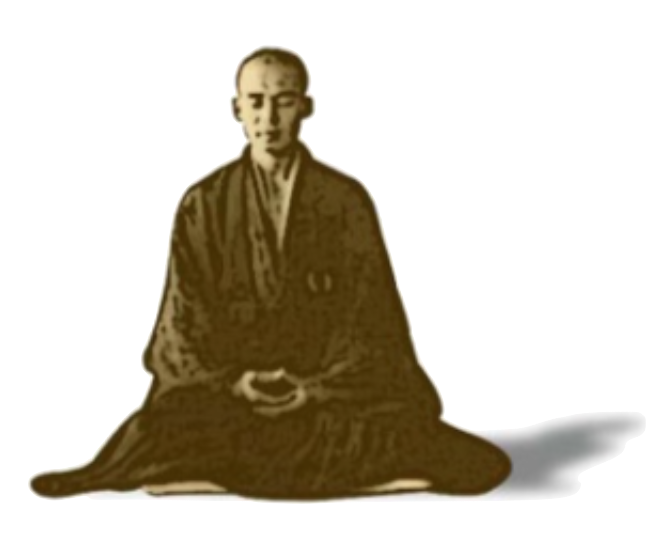
\includegraphics[width=0.3\textwidth]{imagenes/imagenes04/T04IM01.png}
\end{figure}
\end{multicols}
\end{myblock}

\vspace{4mm}
\begin{ejem}
Calcula:  $\left|
\begin{matrix}
1&2&3&4\\-1& \boldsymbol{0}&1&2\\2&\boldsymbol{0}&1&1\\2&2&-2&3&	
\end{matrix}    
\right|=\; [F4 \to F4-F1]\; =$	

$\left|
\begin{matrix}
1&2&3&4\\-1&\boldsymbol{0}&1&2\\2&\boldsymbol{0}&1&1\\1&\boldsymbol{0}&-5&1&	
\end{matrix}    
\right|= 2 \; (-1)^{1+2} \; \left|
\begin{matrix}
-1&1&2\\2&1&1\\1&-5&-1
\end{matrix}    
\right|= \text{ (Sarrus) }=$

$ = 2\; (-1)\; (-23) = \boldsymbol{46}$

\vspace{4mm}
\underline{Observación 1}: No confundir las propiedades de los determinantes por las transformaciones de Gauss: Gauss permite cambiar una fila por un número ($\neq 0$) multiplicada por ella más un número por otra; en los determinantes se puede cambiar una fila (o columna) por `ella misma' (multiplicada por `+1') más un número por otra fila (o columna). \underline{La línea a cambiar} \underline{en un determinante no puede estar multiplicada por ningún número distinto} \underline{ de la unidad positiva} (ni siquiera se puede tomar para restar)  

\footnotesize{\textcolor{gris}{$\begin{array}{lll} *\; \* Fi \to Fi-3Fj \quad \text{Bién} \\
 *\; \* Fi \to 3Fj-Fi \quad \text{Mal: }\; (-1)\cdot Fi \\
  *\; \* Fi \to 2Fi+3Fj \quad \text{Mal: }\; 2\cdot Fi \end{array}$}}\normalsize{.}

\underline{Observación 2}: Hay una gran diferencie entre el producto de un número por una matriz $k\cdot(A)$, en que se multiplican TODOS los elementos de la matriz por $k$ y el producto de un número por un determinantes, $k\cdot |A|$, que consiste en elegir UNA SOLA LÍNEA de $A$ (fila o columna) y multiplicar sus elementos por $k$ (recuérdese lo dicho en la propiedad P.D. 6 de determinantes).

\underline{Observación 3}: Para buscar `ceros' en una columna, combinamos filas. Para buscar `ceros' en una fila, combinamos columnas (Ver en problemas resueltos).

\end{ejem}


\vspace{10mm}
\begin{myexampleblock}{Aplicaciones geométricas de los determinantes}

%\vspace{10mm}
\begin{figure}[H]
	\centering
	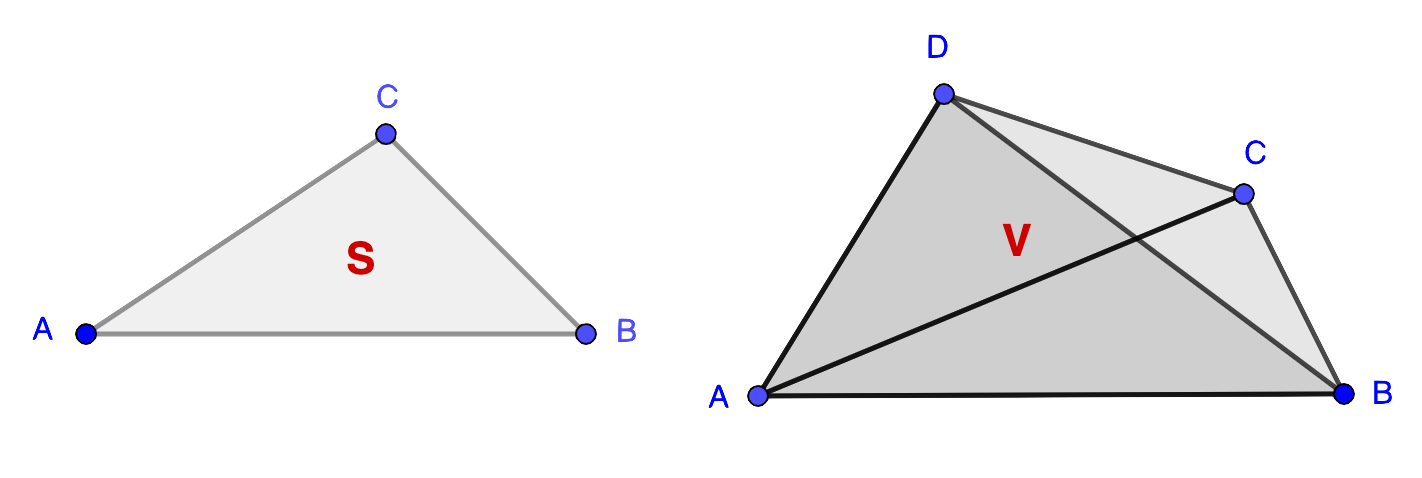
\includegraphics[width=1\textwidth]{imagenes/imagenes04/T04IM04.png}
\end{figure}

Área del triángulo de vértices $A(x_1,y_1),\; B(x_2,y_2),\; C(x_3,y_3)$

Sea $\Delta = \left| \begin{matrix} x_1&x_2&x_3 \\ y_1&y_2&y_3\\1&1&1 \end{matrix} \right|$, entonces, 

Área $S_{ABC}= \dfrac 1 2 \; abs \; \Delta = \dfrac 1 2 \;|\Delta|$ (la mitad del valor absoluto del determinante $\Delta$).

Volumen de un tetraedro de vértices  $A(x_1,y_1,z_1),\; B(x_2,y_2,z_2),$

\noindent $C(x_3,y_3,z_3), \; D(x_4,y_4,z_4)$.

\centerline{Vol. $V=\dfrac 1 6\; abs\; \left( \left| \begin{matrix} x_1&y_1&z_1&1 \\   x_2&y_2&z_2&1  \\  x_3&y_3&z_3&1  \\  x_4&y_4&z_4&1  \end{matrix} \right| \right)$}

\end{myexampleblock}



\justify




\section{Inversa de una matriz por adjuntos}

Ea ahora cuando vamos a desarrollar un método más potente que el de Gauss para el cálculo de la inversa de una matriz cuadrada. Además, este método nos dice si dada una matriz cuadrada cualquiera tiene inversa. (Lo exponemos como un teorema sin demostración).

\begin{teor}{Inversa por adjuntos.}

$\forall A\in \mathcal M_{n \times n}(\mathbb R): \; \exists A^{-1} \Leftrightarrow |A|\neq 0 \; \text{ además }	\;$ \colorbox{LightYellow}{$\boxed{\; A^{-1}=\dfrac 1 {|A|}\; ad(A^T)\; }$}

La inversa de una matriz es uno partido por su determinante \textcolor{gris}{(claro, si el determinantes es cero, no hay inversa)} de la matriz adjunta de la matriz traspuesta. --Puesto que las operaciones de trasposición y adjunto conmutan (se puede comprobar, hágase) algunos autores hablan de la traspuesta de la matriz adjunta-- $[\;ad(A^T)=(ad A)^T \;]$.
\end{teor}

\begin{defi}
Dada $A\in \mathcal M_{n}:$

si $|A|=0 \to \nexists A^{-1} \Rightarrow $ se dice que $A$ es `singular'.

si $|A|\neq 0 \to \exists A^{-1} \Rightarrow $ se dice que $A$ es `regular o invertible'.
\end{defi}


\begin{ejem}
	En el tema anterior, en el apartado de calculo de inversas de matrices por Gauss, vimos:
	
	$B=\left[\begin{matrix} 1&0&2\\3&1&-1\\-2&1&5  \end{matrix}\right] \to B^{-1}=
\dfrac 1 {16} \left[ \begin{matrix} 6&2&-2 \\ -13&9&7 \\5&-1&1  \end{matrix} \right]$

Comprobemos que obtenemos el mismo resultado por el método de los adjuntos:  $B^{-1}=\dfrac 1 {|B|}\; ad(B^T)$:

El \underline{primer caso} es calcular $|B|$, puesto que si es $0$ la matriz será singular o no invertible y habríamos acabado.

Por Sarrus: $|B|=5+6+0-(-4-1+0)=11-(-5)=16\neq 0 \to \exists B^{-1}$

El \underline{segundo paso} es calcular la traspuesta de $B$, no se nos vaya a olvidar \textcolor{gris}{(se puede calcular después del cálculo de la matriz adjunta, como hemos dicho anteriormente, puesto que trasposición y adjunto son operaciones que conmutan)}

$B^T=\left[\begin{matrix} 1&3&-2\\0&1&1\\2&-1&5  \end{matrix}\right]$. Como \underline{tercer paso}, vamos a calcular $ad(B^T)$


$B^T_{11}= (-1)^{1+1}\; \left| \begin{matrix} 1&1\\-1&5 \end{matrix} \right|=
(5-(-1))=6$

$B^T_{12}= (-1)^{1+2}\; \left| \begin{matrix} 0&1\\2&5 \end{matrix} \right|=
-(0-(2))=2$

$B^T_{13}= (-1)^{1+3}\; \left| \begin{matrix} 0&1\\2&-1 \end{matrix} \right|=
(0-(2))=-2$



$B^T_{21}= (-1)^{2+1}\; \left| \begin{matrix} 3&-2\\-1&5 \end{matrix} \right|=
-(15-(2))=-13$

$B^T_{22}= (-1)^{2+2}\; \left| \begin{matrix} 1&-2\\2&5 \end{matrix} \right|=
(5-(-4))=9$

$B^T_{23}= (-1)^{2+3}\; \left| \begin{matrix} 1&3\\2&-1 \end{matrix} \right|=
-(-1-(6))=7$


$B^T_{31}= (-1)^{3+1}\; \left| \begin{matrix} 3&-2\\1&1 \end{matrix} \right|=
(3-(-2))=5$

$B^T_{32}= (-1)^{3+2}\; \left| \begin{matrix} 1&-2\\0&1 \end{matrix} \right|=
-(1-(0))=-1$

$B^T_{33}= (-1)^{3+3}\; \left| \begin{matrix} 1&3\\0&1 \end{matrix} \right|=
(1-(0))=1$

Por lo que $B^{-1}=
\dfrac 1 {16} \left[ \begin{matrix} 6&2&-2 \\ -13&9&7 \\5&-1&1  \end{matrix} \right]$, que coincide con la calculada por el método de Gauss, como era de esperar.

\end{ejem}

\underline{Nota}: Hemos llamado $A$ a una matriz (cuadrada), $a_{ij}$ a sus elementos; $M_{ij}$ a sus menores y $A_{ij}$ a sus adjuntos. El problema surge cuando hablemos de matrices $M$. Proponemos la solución de que $m_{ij}$ sean sus elementos, $M_{ij}$ los menores, entonces a los adjuntos les llamaremos $\boldsymbol{M}_{ij}$ ó $ad_{ij}$.

\begin{figure}[]
	\centering
	
\includegraphics[width=0.8\textwidth]{imagenes/imagenes04/T04IM02.png}
\end{figure}

\begin{teor}{Propiedades de la matiz inversa}

Recordemos las propiedades de la matriz inversa vistas en el capítulo anterior:

Definición:  $AA^{-1}=A^{-1}A=I\quad $
Cálculo: $A^{-1}=\dfrac 1 {|A|}\; ad(A^T)$

\begin{multicols}{2}
\begin{enumerate}
\item $(A^{-1})^{-1}=A$
\item $(k\cdot A)^{-1}= \dfrac 1 k \; A^{-1}$
\item $(A\cdot B)^{-1}=B^{-1} \cdot A^{-1}$
\item $(A^T)^{-1}=(A^{-1})^T$
\end{enumerate}
\end{multicols}
\end{teor}

\subsection{Ecuaciones matriciales}

Son ecuaciones y sistemas en que las incógnitas (y quizás también los coeficientes) son matrices. $X,\; Y, \; \cdots $ son matrices incógnita, $A,\; B, \; C, \; \cdots $ son datos (matrices).

Este tipo de ejercicios constará usualmente  de dos partes: despejar teóricamente la incógnita (si es posible) y realizar las operaciones indicadas a que se ha llegado al despejar.

--- * Sistemas de ecuaciones matriciales lineales:

$\begin{cases} aX+bY=M\\cX+dY=N \end{cases}$, con $a,b,c,d \in \mathbb R$, coeficientes reales y $X,Y,M,N \in \mathcal M (\mathbb R)$, siendo $X$ e $Y$ las matrices incógnita y $M$ y $N$ matrices conocidas (datos).

Se resuelven, teóricamente, como si se tratase de sistemas de ecuaciones lineales cualesquiera y, es después, cuando se realizan las operaciones matriciales necesarias para la solución del sistema.

\begin{ejem} Resuelve $\begin{cases} X-2Y=\left( \begin{matrix}  1&0\\1&1 \end{matrix} \right) \\ X+3Y=\left( \begin{matrix}  0&2\\4&-3 \end{matrix} \right) \end{cases}$ 

Si a la segunda ecuación le restamos la primera: 

$\boldsymbol{Y}=\left( \begin{matrix}  0&2\\4&-3 \end{matrix} \right) -\left( \begin{matrix}  1&0\\1&1 \end{matrix} \right)=\boldsymbol{ \left( \begin{matrix} -1&2 \\3&-4  \end{matrix}  \right)}$

Sustituyendo en la primera ecuación:
$\boldsymbol{ X}=\left( \begin{matrix}  1&0\\1&1 \end{matrix} \right)+2Y=$

$=\left( \begin{matrix}  1&0\\1&1 \end{matrix} \right)+2\left( \begin{matrix} -1&2 \\3&-4  \end{matrix}  \right)=
\left( \begin{matrix}  1&0\\1&1 \end{matrix} \right)
+\left( \begin{matrix} -2&4 \\6&-8  \end{matrix}  \right)=
\boldsymbol{ \left( \begin{matrix}  -1&4\\7&-7 \end{matrix} \right)}$

\end{ejem}

--- * Ecuaciones matriciales: 

Son ecuaciones en que tanto coeficientes como incógnitas son matrices.

$AX=B \to \text{ si } \exists A^{-1} \; \therefore \; $ `premultiplicando por $A^{-1}$:

$A^{-1}(AX)= A^{-1}(B) \to A^{-1}AX=IX=\boldsymbol{A=A^{-1}B}$

Solo quedaría, en un problema usual, hacer las operaciones que han aparecido al despejar. En este caso, calcular la inversa de $A$ y `premultiplicar' por $B$ 

\underline{¡Ojo!}: el orden en que se multiplican matrices es MUY importante, por eso insistimos en lo de `premultiplicar' y `postmultiplicar' 

Veamos otros ejemplos teóricos de resolución de ecuaciones matriciales:

\noindent * $XM=N \to$

Si $\exists M^{-1}$, postmultiplicando: $XMM^{-1}=XI=\boldsymbol{X=NM^{-1}}$

\noindent * $AXB=C \to $

Si existen $A^{-1}$ y $B^{-1}$, premultiplicando por $A^{-1}$ y postmultiplicando por $B^{-1}$ (lo hacemos más explícitamente en este caso):

$\textcolor{red}{A^{-1}} \cdot \textcolor{blue}{AXB}  \cdot \textcolor{red}{B^{-1}}= $
$\textcolor{red}{A^{-1}} \cdot \textcolor{blue}{C} \cdot \textcolor{red}{B^{-1}} $
$\to A^{-1}AXBB^{-1}=A^{-1}CB^{-1} \to $

$IXI=A^{-1}CB^{-1} \Rightarrow X=A^{-1}CB^{-1}$

\noindent * $ABX=C \to $

Si existen $A^{-1}$ y $B^{-1}$, premultiplicando por $A^{-1}$ y luego por $B^{-1}$:

$ \textcolor{red}{A^{-1}} ABX = \textcolor{red}{A^{-1}} C \to  A^{-1}ABX=A^{-1}C\to IBX=A^{-1}C \Rightarrow$ 

$BX=A^{-1}C$. Ahora por $B^{-1}\; $: $\textcolor{blue}{B^{-1}}BX=\textcolor{blue}{B^{-1}}A^{-1}C \to $

$BB^{-1}X=B^{-1}A^{-1}C \to IX=B^{-1}A^{-1}C  \Rightarrow X=B^{-1}A^{-1}C $

Obsérvese que también podíamos haber hecho: $(AB)X=C$, si existe $(AB)^{-1} \to (AB)^{-1}(AB)X=(AB)^{-1}C \to IX=(AB)^{-1}C \qquad  \Rightarrow \qquad X=(AB)^{-1}C$, que evidentemente es el mismo resultado anterior, puesto que $(AB)^{-1}=B^{-1}A^{-1}$

\noindent * $AX=BX+C \to$ 

Primero aislemos la matriz incógnita $X$ en un solo miembro de la ecuación:

$AX-BX=C \to (A-B)X=C \to \text{ si } \; \exists (A-B)^{-1} \quad  \therefore \; $

$(A-B)^{-1}(A-B)X=(A-B)^{-1}C \to IX=(A-B)^{-1}C \Rightarrow $

$X=(A-B)^{-1}C$

\noindent * $XM=NX+P \to$ 

Como en el caso anterior: $XM-NX=P$, sacando `factor común por la izquierda':

$X(M-N)=P$, si existe $(M-N)^{-1}$, postmultiplicando en ste caso:

$X(M-N)(M-N)^{-1}=P(M-N)^{-1} \to XI=P(M-N)^{-1} \Rightarrow $

$X=P(M-N)^{-1}$

\noindent * $XM=2X+N$

Análogamente al caso anterior: $XM-2X=N \to X(M-2)= \cdots $ ¡Un momento!: $M-2$ no tiene ningún sentido. ASTUCIA: usemos la matriz $I$:

\small{$XM-2X=N \to XM-X2=N \to XM-X2\textcolor{red}{I}=N \to X(M-2I)=N$}\normalsize{.}

Si existe la inversa de la matriz $M-2I$, que ahora sí tiene sentido, postmultiplicando tendremos:

$X(M-2I)(M-2I)^{-1}=N(M-2I)^{-1} \to XI=N(M-2I)^{-1} \Rightarrow $

$X=N(M-2I)^{-1}$

\noindent * etc.  En problemas veremos, y resolveremos, más casos.





\subsection{Forma matricial de un SEL}

Un sistema de ecuaciones lineales `cuadrado', es decir, con tantas ecuaciones como incógnitas, se puede interpretar como una ecuación matricial:

$\begin{cases} a_{11}x_1+a_{12}x_2 + \cdots + a_{1n}x_n &=b_1 \\
a_{12}x_1+a_{22}x_2 + \cdots + a_{2n}x_n &=b_2 \\
\cdots + \cdots + \cdots + \cdots + \cdots  &=\cdots \\
a_{n1}x_1+a_{n2}x_2+\cdots +a_{nn}x_n &=b_n  \end{cases} \quad \Leftrightarrow \quad \boxed{\; AX=B\; \; }$	,

donde:
$A=\left( \begin{matrix}  a_{11}&a_{12}& \cdots &a_{1n} \\
a_{12} &a_{22} &\cdots &a_{2n} \\
\cdots & \cdots & \cdots & \cdots  \\
a_{n1} &a_{n2} &\cdots &a_{nn}    \end{matrix} \right); \; X=\left( \begin{matrix} x_1\\x_2\\ \vdots \\x_n \end{matrix} \right); \; B=\left( \begin{matrix} b_1\\b_2\\ \vdots \\b_n \end{matrix} \right)$

$A$ es la matriz de los coeficientes, $X$ la de incógnitas y $B$ la de términos independientes.

Es decir: 

\noindent \colorbox{LightYellow}{\scriptsize{$\boxed{\begin{cases} a_{11}x_1+a_{12}x_2 + \cdots + a_{1n}x_n &=b_1 \\
a_{12}x_1+a_{22}x_2 + \cdots + a_{2n}x_n &=b_2 \\
\cdots + \cdots + \cdots + \cdots + \cdots  &=\cdots \\
a_{n1}x_1+a_{n2}x_2+\cdots +a_{nn}x_n &=b_n  \end{cases}  \Leftrightarrow 
\left( \begin{matrix}  a_{11}&a_{12}& \cdots &a_{1n} \\
a_{12} &a_{22} &\cdots &a_{2n} \\
\cdots & \cdots & \cdots & \cdots  \\
a_{n1} &a_{n2} &\cdots &a_{nn}    \end{matrix} \right) \cdot \left( \begin{matrix} x_1\\x_2\\ \vdots \\x_n \end{matrix} \right)=\left( \begin{matrix} b_1\\b_2\\ \vdots \\b_n \end{matrix} \right)}$}}

\normalsize{En} el caso de que $\exists A^{-1}$, se puede resolver la ecuación matricialemente.

Consideraciones: para usar este método es necesario que el sistema sea cuadrado y la matriz de los coeficientes sea distinta de cero (para que $\exists A^{-1}$. Además, el cálculo de una inversa suele ser largo. El método de Gauss sirve para cualquier sistema de ecuaciones.

En el apartado de problemas veremos como resolver matricialmente un SEL.



\section{Ejercicios}

\subsection{Ejercicios resueltos}

%Cálculo Sarrus-Laplace

\begin{ejre} Calcula:

\noindent \small{$a)\; \left| \begin{matrix} 2&-1\\8&5  \end{matrix} \right| \; \;    
b)\; \left| \begin{matrix} -2&1&3\\5&-1&0\\0&2&-6  \end{matrix} \right| \; \; 
c)\; \left| \begin{matrix} 2&1&0&-1\\3&1&2&-1\\2&-1&1&0\\0&1&1&2  \end{matrix} \right| \; \; 
d)\; \left| \begin{matrix} 1&-1&0&2&0\\1&0&2&0&0\\0&0&-1&2&3\\-1&2&2&-1&0\\2&5&0&1&-2   \end{matrix} \right| \; \; $}

\end{ejre}

\begin{proofw}\renewcommand{\qedsymbol}{$\diamond$}

\normalsize{-----} a) $\left| \begin{matrix} 2&-1\\8&5  \end{matrix} \right|=10-(-8)=\boldsymbol{ 18}$	

\noindent ----- b) $\left| \begin{matrix} -2&1&3\\5&-1&0\\0&2&-6  \end{matrix} \right|= -12+30+0-(0+0-30)=\boldsymbol{48}$


\noindent ----- c) $\left| \begin{matrix} 2&1&0&-1\\3&1&2&-1\\2&-1&1&0\\0&1&1&2  \end{matrix} \right| = \left[ \begin{matrix} F2 \to F2-2F4\\ F3 \to F3-F4 \end{matrix} \right] = \left| \begin{matrix} 2&1&\boxed{0}&-1\\3&-1&\boxed{0}&-5\\2&-2&\boxed{0}&-2\\0&1&1&2  \end{matrix} \right| =\to $

Desarrollamos por Laplace por los adjuntos de la tercera columna:

\noindent $\to = 0\; +\; 0\; +\; 0\; +\; 1\cdot (-1)^{4+3} \left| \begin{matrix} 2&1&-1\\3&-1&-5\\2&-2&-2 \end{matrix} \right| = - [\; 4+6-10-(2+20-6) \; ]= -[0-(16)]=\boldsymbol{ 16} $

\noindent ----- d) $ \left| \begin{matrix} 1&-1&0&2&\boldsymbol{0}\\1&0&2&0&\boldsymbol{0}\\0&0&-1&2&3\\-1&2&2&-1&\boldsymbol{0}\\2&5&0&1&-2   \end{matrix} \right| =  \dfrac {\colorbox{Yellow}{3}} {3}  \left| \begin{matrix} 1&-1&0&2&\boldsymbol{0}\\1&0&2&0&\boldsymbol{0}\\0&0&-1&2&3\\-1&2&2&-1&\boldsymbol{0}\\\colorbox{Yellow}{2}&\colorbox{Yellow}{5}&\colorbox{Yellow}{0}&\colorbox{Yellow}{1}&\colorbox{Yellow}{-2}   \end{matrix} \right|= \to  $

Multiplicamos, y dividimos, la última fila por $3$, para tenerla preparada y buscar `ceros en la quinta columna): \textcolor{gris}{(también hubiésemos podido buscar `ceros' en la segunda fila, donde ya hay $3$, cambiando $C2$ por$C2-2C1$)}

\noindent $\dfrac 1 3  \left| \begin{matrix} 1&-1&0&2&\boldsymbol{0}\\1&0&2&0&\boldsymbol{0}\\0&0&-1&2&3\\-1&2&2&-1&\boldsymbol{0}\\\colorbox{Yellow}{6}&\colorbox{Yellow}{15}&\colorbox{Yellow}{0}&\colorbox{Yellow}{3}&\colorbox{Yellow}{-6}   \end{matrix} \right|= 
[\;F5 \to F5+2F3\;] = \to $

\noindent $\dfrac 1 3  \left| \begin{matrix} 1&-1&0&2&\text{\textst{ 0 }}	\\1&0&2&0&\text{\textst{ 0 }}	\\\text{\textst{ 0 }}	&\text{\textst{ 0 }}	&\text{\textst{ -1 }}	&\text{\textst{ 2 }}	&\text{\textst{ 3 }}	\\-1&2&2&-1&\text{\textst{ 0 }}	\\6&15&-2&7&\text{\textst{ 0 }}	   \end{matrix} \right|= $ (Laplace $5^a$ columna) $=\to$

\noindent $\to =0\; +\; 0\; + \dfrac 1 3\; 3 \cdot (-1)^{3+5} \left|
\begin{matrix}   1&-1&0&2\\1&\boldsymbol{ 0}&2&\boldsymbol{ 0}\\-1&2&2&-1 \\6&15&-2&7  \end{matrix} \right| = [\; C3 \to C3-2C1 \;  ] = \to $

\noindent $=+\left|
\begin{matrix}   1&-1&-2&2\\1&\boldsymbol{ 0}&\boldsymbol{0} &\boldsymbol{ 0}\\-1&2&4&-1 \\6&15&-14&7  \end{matrix} \right|=$  (Lapalace $2^a$ fila) 
$=   \left|
\begin{matrix}   \text{\textst{ 1 }}&-1&-2&2\\\text{\textst{ 1 }}&\text{\textst{ 0 }}&\text{\textst{ 0 }} &\text{\textst{ 0 }}\\\text{\textst{ 1 }}&2&4&-1 \\\text{\textst{ 6 }}&15&-14&7  \end{matrix} \right| = $


\noindent $1\cdot (-1)^{2+1}\; \left| \begin{matrix}  -1&-2&2\\2&4&-1\\15&-14&7 \end{matrix} \right| +0+0+0= -[-28-56+30-(120-14-28)]=-[-54-(78)]-[-132]=\boldsymbol{132}$
\end{proofw}


\begin{ejre}
Dada $A=\left[ \begin{matrix}2&3&0\\0&1&2\\-1&0&2 \end{matrix} \right]\;$, calcula los siguientes adjuntos: $A_{23}; \; A_{32}; \; A_{11}$
\end{ejre}

\begin{proofw}\renewcommand{\qedsymbol}{$\diamond$}

$A_{23}=(-1)^{2+3}\;M_{23}= (-1)\; \left| \begin{matrix} 2&3\\-1&0
 \end{matrix} \right|= (-1)\; (0-(-3)) = \boldsymbol{-3}$
 
\noindent $A_{32}=(-1)^{3+3}\;M_{32}= (-1)\; \left| \begin{matrix} 2&0\\0&2
 \end{matrix} \right|= (-1)\; (4-(0)) = \boldsymbol{-4}$	
 
\noindent $A_{11}=(-1)^{1+1}\;M_{1}= +\; \left| \begin{matrix} 1&2\\0&2
 \end{matrix} \right|=  (2-(0)) = \boldsymbol{2}$
\end{proofw}

\begin{ejre}
	Sea $\; A_n=\left( \begin{matrix}
 1&1&1&\cdots&1 \\ -1&2&1&\cdots &1	\\ -1&-1&2&\cdots &1 \\ \vdots & \vdots & \vdots & \ddots & \vdots \\-1&-1&-1& \cdots &2
 \end{matrix} \right)\; $. 
 
 Calcula $det(A_2); \; det(A_3); \; det(A_4)$. ¿Qué valdrá el $\; det(A_n)\; $?

\end{ejre}

\begin{proofw}\renewcommand{\qedsymbol}{$\diamond$}
	$A_2= \left| \begin{matrix} 1&1\\-1&2   \end{matrix} \right|=2-(-1)=3=3^{2-1}$
	
\noindent $A_2= \left| \begin{matrix} 1&1&1\\-1&2&1 \\ -1&-1&2   \end{matrix} \right|=4+1-1 -(-2-1-2) =4-(-5)=9=3^2=3^{3-1}$

\noindent $A_3= \left| \begin{matrix} 1&1&1&1\\-1&2&1&1 \\ -1&-1&2&1 \\ -1&-1&-1&2   \end{matrix} \right|= \textcolor{gris}{\begin{cases} F2\to F1+F1 \\ F3\to F3+F1  \\ F4\to F4+F1  \end{cases}} = 
\left| \begin{matrix} 1&1&1&1\\0&3&2&2 \\ 0&0&3&2 \\ 0&0&0&3   \end{matrix} \right| = \textcolor{gris}{diagonal}= 1\cdot 3 \cdot 3 \cdot 3=27=3^3=3^{4-1}$

\noindent Conjeturamos que $det(A_n)=|A_n|=3^{n-1}\; $ Habría que demostrarlo por inducción (ver apéndice \ref{inducción}).
		
\end{proofw}

\begin{ejre}
Calcula:  $\;  \left| \begin{matrix} 1&ln 2&(ln 2)^2\\ 1 & ln 4 & (ln 4)^2 \\ 1& ln 8 & (ln 8)^2  \end{matrix} \right| \;$	
\end{ejre}

\begin{proofw}\renewcommand{\qedsymbol}{$\diamond$}

\noindent Es sabido que: $ln x - ln y = ln \frac x y \to \begin{cases}
 ln 4-ln 2= ln \frac 4 2 = ln 2 \\ ln8-ln2=ln \frac 8 2 = ln 4=ln 2^2=2ln 2	
 \end{cases}$
 
\noindent Tambien que $ln x + ln y = ln (x\cdot y)$, así como $ln x^n=n\;lnx$
 
\noindent Y que: $a^2-b^2=(a+b)(a-b) \to \begin{cases}
 (ln4)^2-(ln2)^2=(ln4+ln2)\cdot (ln4-ln2)=\\
 =ln8\cdot ln 2= ln2^3\cdot ln2=3(ln2)^2	\\
 ----------\\
 (ln 8)^2-(ln2)^2=(ln8+ln2)\cdot(ln8-ln2)=\\
 =ln16\cdot ln4=ln2^4\cdot ln2^2=8(ln2)^2
 \end{cases}$

\noindent $\;  \left| \begin{matrix} 1&ln 2&(ln 2)^2\\ 1 & ln 4 & (ln 4)^2 \\ 1& ln 8 & (ln 8)^2  \end{matrix} \right| \; = \textcolor{gris}{\left[ \begin{matrix} F2\to F2-F1\\ F3 \to F3-F1  \end{matrix} \right]} = \;  \;  \left| \begin{matrix} 1&ln 2&(ln 2)^2\\ 1 & ln 2 & 3(ln 2)^2 \\ 1& 2ln 2 & 8(ln 2)^2  \end{matrix} \right| \; = \textcolor{gris}{ \begin{cases} ln2 \text { factor común } C2\\  (ln2)^2 \text { factor común } C3 \end{cases} }\; =  (ln2)^3\;  \left| \begin{matrix}  1&1&1\\0&1&3\\0&2&8 \end{matrix} \right| \; = \textcolor{gris}{[ F3\to F3-2F2 ]}= (ln2)^3\; \left| \begin{matrix} 1&1&1\\0&1&3\\0&0&2  \end{matrix} \right|\; \textcolor{gris}{\text{ diagonal }}\; = (ln2)^3 1\cdot 1\cdot 2= \boldsymbol{2(ln 2)^3} $
	
\end{proofw}

%$ \left| \begin{matrix}   \end{matrix} \right|$

% Propiedades

\begin{ejre}
	Calcula: $\; \left| \begin{matrix} a&a&a\\-a&a&x\\ -a&-a&x  \end{matrix} \right| $
\end{ejre}

\begin{proofw}\renewcommand{\qedsymbol}{$\diamond$}
	$\left| \begin{matrix} a&a&a\\-a&a&x\\ -a&-a&x  \end{matrix} \right|=
	\textcolor{gris}{\left[ \begin{matrix} F2\to F2+F1\\ F3\to F3+F1  \end{matrix}  \right]}=\left| \begin{matrix} a&a&a\\0&2a&x+a\\ 0&0&x+a  \end{matrix} \right|= \; \textcolor{gris}{( diagonal )} \; =$
	
\noindent 	$=\boldsymbol{ 2a\cdot(x+a)^2 } $
\end{proofw}

\begin{ejre}
Calcula: 	$\; \left| \begin{matrix}  a&a&a&a\\a&b&b&b\\a&b&c&c\\a&b&c&d \end{matrix} \right|$
\end{ejre}

\begin{proofw}\renewcommand{\qedsymbol}{$\diamond$}
$\left| \begin{matrix}  a&a&a&a\\a&b&b&b\\a&b&c&c\\a&b&c&d \end{matrix} \right| \;=\; \textcolor{gris}{\left[ \begin{matrix} F2\to F2-F1 \\F3\to F3-F1  \\F4\to F4-F1  \end{matrix} \right]} \;=\; 
\left| \begin{matrix}  a&a&a&a\\0&b-a&b-a&b-a\\0&b-a&c-a&c-a\\0&b-a&c-a&d-a \end{matrix} \right| \; = \; 
\textcolor{gris}{ \left[ \begin{matrix}
a \text{ factor común F1} \\ (b-a) \text{ factor común F2}  \end{matrix} \right] }=\quad  a\cdot (b-a)\; \left| \begin{matrix}  1&1&1&1\\0&1&1&1\\0&b-a&c-a&c-a\\0&b-a&c-a&d-a \end{matrix} \right| 
=\quad \textcolor{gris}{\left[ \begin{matrix} F3\to F3-(b-a)F2 \\F4\to F4-(b-a)F2   \end{matrix} \right]}=a\cdot (b-a)\; \left| \begin{matrix}  1&1&1&1 \\ 0&1&1&1 \\ 0&0&c-b&c-b \\ 0&0&c-b&d-b \end{matrix} \right| = \small{\textcolor{gris}{(F4 \to F4-F3)}}\normalsize{=}$
  
\noindent $=\left| \begin{matrix}  1&1&1&1 \\ 0&1&1&1 \\ 0&0&c-b&c-b \\ 0&0&0&d-c \end{matrix} \right| = \textcolor{gris}{\text{ (diagonal) }}=\boldsymbol{ a(b-a)(c-b)(b-c) }$	
\end{proofw}

\begin{ejre}
Sabiendo que $\left| \begin{matrix} a&1&d\\b&2&d\\c&3&d \end{matrix} \right|=5\;$ encuentra el valor de los siguientes determinantes:

$a)\; \left| \begin{matrix} a+2d&2&d\\b+2d&4&d\\c+2d&6&d  \end{matrix} \right|; \;\;
b)\; \left| \begin{matrix} a&3d&-1-2a\\b&3d&-2-2b\\c&3d&-3-2c  \end{matrix} \right|; \;\;
c)\; \left| \begin{matrix} 6&2&3\\a+b+c&b&c\\3d&d&d  \end{matrix} \right| =$
 
\end{ejre}

\begin{proofw}\renewcommand{\qedsymbol}{$\diamond$}

--- a) $\left| \begin{matrix} a+2d&2&d\\b+2d&4&d\\c+2d&6&d  \end{matrix} \right|=\left| \begin{matrix} a&2&d\\b&4&d\\c&6&d  \end{matrix} \right|\;    + \; \cancelto{0}{ \left| \begin{matrix} 2d&2&d\\2d&4&d\\2d&6&d  \end{matrix} \right|}= $
\small{$[C1 \text{ proporc. } C3 ]$}\normalsize{$=$}
$=2\; \left| \begin{matrix} a&1&d\\b&2&d\\c&3&d  \end{matrix} \right| =$
\small{$[2$ factor común $C2]$}\normalsize{$=$}$2\cdot 5=$ \small{[por hipótesis]} \normalsize{$=\boldsymbol{10} $}

\noindent ---b) $\left| \begin{matrix} a&3d&-1-2a\\b&3d&-2-2b\\c&3d&-3-2c  \end{matrix} \right|=- \left| \begin{matrix} a&3d&1\\b&3d&2\\c&3d&3  \end{matrix} \right|
- \cancelto{0}{\left| \begin{matrix} a&3d&2a\\b&3d&2b\\c&3d&2c  \end{matrix} \right|} =$ \small{$[C3 \text{ proporc. } C1 ]$}\normalsize{$=$}
$=- 3\; \left| \begin{matrix} a&d&1\\b&d&2\\c&d&3  \end{matrix} \right|=$ 
\small{$[ 3$ factor común $C2]$}\normalsize{$=$} 
$=- 3\;(-1)\; \left| \begin{matrix} a&1&d\\b&2&d\\c&3&d \end{matrix} \right|=$ 

\noindent \small{Intercambio $C2 \leftrightarrow C3$}\normalsize{$=$} 
$(-3)(-1)\; 5 $ \small{[por hipótesis]}\normalsize{$=$}$\boldsymbol{15}$ 

\noindent --- c) $\left| \begin{matrix} 6&2&3\\a+b+c&b&c\\3d&d&d  \end{matrix} \right|= (\;*\;)=
 \left| \begin{matrix} 1+2+3&2&3\\a+b+c&b&c\\d+d+d&d&d  \end{matrix} \right|=$

\noindent \normalsize{$=$} \small{[rompemos como suma de tres determinantes]}\normalsize{$=$}

\noindent $=
 \left| \begin{matrix} 1&2&3\\a&b&c\\d&d&d  \end{matrix} \right|+
  \cancelto{0}{\left| \begin{matrix} 2&2&3\\b&b&c\\d&d&d  \end{matrix} \right|}+
   \cancelto{0}{\left| \begin{matrix} 3&2&3\\c&b&c\\d&d&d  \end{matrix} \right|}=$ \small{$\left[ \begin{matrix} 
\text{det-2: } C1=C2 \\
\text{det-3: } C1=C3 \\
\text{det-1: } |A|=|A^t| 
\end{matrix} \right]$}\normalsize{$=$}

\noindent $=\left| \begin{matrix} 1&a&d\\2&b&d\\3&c&d  \end{matrix} \right| =$
\small{[Intercambio: $C1 \leftrightarrow C2$]} \normalsize{$=$}
$-\left| \begin{matrix} a&1&d\\b&2&d\\c&3&d  \end{matrix} \right| = \boldsymbol{-5}$, \small{por hipótesis}\normalsize{.}

\end{proofw}

%$ \left| \begin{matrix}   \end{matrix} \right|$

\begin{ejre}
Sean $A$ y $B$ dos matrices cuadradas de orden $3$ tales que $|A|=4$ y $|B|=2$. Calcula:

$a)\; |AB|; \quad b)\; |(A^TB)^{-1}|; \quad c)\; |A^3B^2|; \quad d)\; |5A|$
\end{ejre}

\begin{proofw}\renewcommand{\qedsymbol}{$\diamond$}
	Usando las propiedades de los determinantes:
	
\noindent --- a) $|AB|=|A|\cdot|B|=4\cdot 2 = \boldsymbol{8} $

\noindent --- b) $|(A^TB)^{-1}|=\dfrac {1}{|A^TB|}= \dfrac {1}{|A^T| \cdot |B|}=\dfrac {1}{|A| \cdot |B|}= \dfrac {1}{4 \cdot 2}= \boldsymbol{\dfrac 1 8}$

\noindent --- c) $|A^3B^2|=|A|^3 \cdot |B|^2=4^3 \cdot 2^2 =\boldsymbol{256}$

\noindent --- d) Como $A$ es de orden $3$:  $\; |5A|=5^3 \; |A| = 5^3 \cdot 4=\boldsymbol{500}$
\end{proofw}

\begin{ejre}
Considera $\;\left| \begin{matrix} 1&1&1\\x&y&z\\0&2&4  \end{matrix} \right|=4\;$, sin usar Sarrus, calcula los siguientes determinantes:

$a)\; \;  \left| \begin{matrix} 3x&3y&3z\\1&1&1\\0&1&2   \end{matrix} \right| \qquad b)\; \; 
 \left| \begin{matrix} x&y&z\\3x&3y+2&3z+4\\x+2&y+2&z+2  \end{matrix} \right|$
\end{ejre}

\begin{proofw}\renewcommand{\qedsymbol}{$\diamond$}

$a)\; \;  \left| \begin{matrix} 3x&3y&3z\\1&1&1\\0&1&2   \end{matrix} \right|=\; $ \textcolor{gris}{(3 factor común F1)} $\; = 3\; \left| \begin{matrix} x&y&z\\1&1&1\\0&1&2   \end{matrix} \right|=\; $ \textcolor{gris}{($F1\leftrightarrow F2$)} $\;= -3\; \dfrac 2 2 \; \left| \begin{matrix} 1&1&1\\x&y&z\\0&1&2   \end{matrix} \right|=\; $ \textcolor{gris}{$2\cdot F3$} $\; = - \dfrac 3 2 \left| \begin{matrix} 1&1&1\\x&y&z\\0&2&4   \end{matrix} \right| =\;$ \textcolor{gris}{(por hipótesis)} $\; = - \dfrac 3 2 4 = \boldsymbol{-6}$

\noindent  $b)\; \; \left| \begin{matrix} x&y&z\\3x&3y+2&3z+4\\x+2&y+2&z+2  \end{matrix} \right| =\; $ \textcolor{gris}{(suma dos determinantes por F3)} $\; = \cancelto{0}{\left| \begin{matrix} x&y&z\\3x&3y+2&3z+4\\x&y&z  \end{matrix} \right|} \; + \; \left| \begin{matrix} x&y&z\\3x\textcolor{red}{+0}&3y+2&3z+4\\2&2&2  \end{matrix} \right| =\; $ \textcolor{gris}{primer det. es cero por F1=F3; segundo determinante como suma de dos por la F2} $\; = \left| \begin{matrix} x&y&z\\3x&3y&3z\\2&2&2  \end{matrix} \right| \; + \; \left| \begin{matrix} x&y&z\\0&2&4\\2&2&2  \end{matrix} \right| =\; $ \textcolor{gris}{(3 factor común primer det. F2; 2 factor común segundo det. F3)} $\; = 3\; \cancelto{0}{ \left| \begin{matrix} x&y&z\\x&y&z\\2&2&2  \end{matrix} \right|} \; + \; 2\; \left| \begin{matrix} x&y&z\\0&2&4\\1&1&1  \end{matrix} \right| =\; $ \textcolor{gris}{(primer determinante es cero por $F1=F2$; segundo determinantes: $F1\leftrightarrow F2$)} $\; =  -2\; \left| \begin{matrix} 0&2&4\\x&y&z\\1&1&1  \end{matrix} \right| =\; $  \textcolor{gris}{($F1 \leftrightarrow F3$)} $\; =  +2\; \left| \begin{matrix} 1&1&1\\x&y&z\\0&2&4  \end{matrix} \right| =\; $ \textcolor{gris}{(por hipótesis)} $\; = 2\cdot 4 = \boldsymbol{8}$

\end{proofw}

\begin{ejre}
Para $\; M=\left( \begin{matrix} 2&1&-1\\1&0&1\\3&1&2 \end{matrix} \right)\; $, calcula 

$|M|; \; |M^T|; \; |M^3|; \; |4M|; \; |M^{-1}|$	
\end{ejre}

\begin{proofw}\renewcommand{\qedsymbol}{$\diamond$}

Por Sarrus, $|M|=-1+3-(2+2)=-2$

\begin{multicols}{2}
\noindent $|M^T|=|M|=-2$

\noindent $|M^3|=|M|^3=(-2)^3=-8$

\noindent $|4M|=4^3\;|M|=4^3\cdot (-2)=-128$

\noindent $|M^{-1}|= \dfrac 1 {|M|}= - \dfrac 1 2$	
\end{multicols}
\end{proofw}


\begin{ejre}
	Sin desarrollar el determinante, prueba que $3,4 \text{ y } -7$ sos raíces del polinomio $P(x)=\left| \begin{matrix} 4&4&x\\3&x&4\\x&3&3 \end{matrix} \right|$
\end{ejre}

\begin{proofw}\renewcommand{\qedsymbol}{$\diamond$}

$P(3)=\left| \begin{matrix} 4&4&3\\3&3&4\\3&3&3 \end{matrix} \right|=0\;$ por tener dos columnas iguales $C1=C2$

\noindent $P(4)=\left| \begin{matrix} 4&4&4\\3&4&4\\4&3&3 \end{matrix} \right|=0\; $ por tener dos columnas iguales $C2=C3$

\noindent $P(-7)=\left| \begin{matrix} 4&4&-7\\3&-7&4\\-7&3&3 \end{matrix} \right|=0\;$ Se observa que $F1+F2+F3=0 \to $

\noindent $F1=-F2-F3$ , por ejemplo. Una fila es combinación lineal de otras, luego su determinante es cero.  \small{De otro modo, si usamos la propiedad que dice `a una línea de un  determinantes se le puede sumar un número por otra línea': $F1\to F1+F2 ; \; $ a la nueva $F1\to F1+F3$, tendríamos que la primera fila son todos sus elementos cero y por la propiedad que dice que `si un determinante tiene una línea de ceros, el determinante es cero', quedaría probado lo que pretendíamos demostrar}\normalsize{.} 

\end{proofw}

\begin{ejre}
	Sin desarrollar, resuelve: $\; \left| \begin{matrix} 1&1&1\\1&x&1\\1&1&x^2  \end{matrix} \right|=0$
\end{ejre}

\begin{proofw}\renewcommand{\qedsymbol}{$\diamond$}
	$\left| \begin{matrix} 1&1&1\\1&x&1\\1&1&x^2  \end{matrix} \right|= \textcolor{gris}{\left[ \begin{matrix} F2\to F2-F1\\ F3\to F3-F1  \end{matrix} \right]}= \left| \begin{matrix} 1&1&1\\0&x-1&0\\0&0&x^2-1  \end{matrix} \right|= \textcolor{gris}{ (diagonal) }= (x-1)(x^2-1)=0 \to \boldsymbol{ x=1\; \wedge \; x=-1}$
\end{proofw}

\begin{ejre} Calcula de determinante de Vandermonde de orden 4: (en el apéndice \ref{Vandermonde} se ve la generalización de este determinante y una de sus múltiples aplicaciones.)

$\left| \begin{matrix} 1&1&1&1\\a&b&c&d\\a^2&b^2&c^2&d^2\\a^3&b^3&c^3&d^3  \end{matrix} \right|$
	
\end{ejre}

\begin{proofw}\renewcommand{\qedsymbol}{$\diamond$}
	$\left| \begin{matrix} 1&1&1&1\\a&b&c&d\\a^2&b^2&c^2&d^2\\a^3&b^3&c^3&d^3  \end{matrix} \right|= 
	\textcolor{gris}{
\left[ \begin{matrix}
 F4\to F4-aF3 \\F3\to F3-aF2\\F2\to F2-aF1	
 \end{matrix} \right] } =  
 \left| \begin{matrix} 1&1&1&1\\0&b-a&c-a&d-a\\0&b^2-ab&c^2-ac&d^2-ac\\0&b^3-ab^2&c^3-ac^2&d^3-ac^2  \end{matrix} \right| = 
 \left| \begin{matrix} 1&1&1&1\\0&b-a&c-a&d-a\\0&b(b-a)&c(a-c)&d(a-d)\\0&b^2(b-a)&c^2(c-a)&d^2(d-a)  \end{matrix} \right|=\to$ 
 
 \noindent \textcolor{gris}{Desarrollo de Laplace por adjuntos de la primera columna} 
 
 \noindent $\to = 1 \; (-1)^{1+1}\; \left| \begin{matrix} b-a&c-a&d-a\\b(b-a)&c(a-c)&d(a-d)\\b^2(b-a)&c^2(c-a)&d^2(d-a)  \end{matrix} \right| \; + 0\; +\; 0\; +\; 0=\to$ 
  
 \noindent \textcolor{gris}{ factor común $\begin{cases} b-a \text{ por} \; C1 \\ c-a \text{ por} \; C2 \\d-a \text{ por} \; C3 \end{cases} $} $\to =
 (b-a)(c-a)(d-a)\left| \begin{matrix}  1&1&1\\b&c&d\\b^2&c^2&d^2 \end{matrix} \right| = \to$
 
\noindent $\to =\textcolor{gris}{
\left[ \begin{matrix}
 F4\to F3-bF2 \\F2\to F2-bF1
 \end{matrix} \right] }= (b-a)(c-a)(d-a)\left| \begin{matrix}  1&1&1\\0&c-b&d-b\\0&c^2-bc&d^2-bd \end{matrix} \right| = \to$ 
 
 \noindent $ = (b-a)(c-a)(d-a)\left| \begin{matrix}  1&1&1\\0&c-b&d-b\\0&c(c-b)&d(d-b) \end{matrix} \right| = \to$
 
 \noindent \textcolor{gris}{Desarrollo de Laplace por adjuntos de la primera columna} 
 
 \noindent $(b-a)(c-a)(d-a)\;1\:(-1)^{1+1}\; \left| \begin{matrix}  c-b&d-b\\c(c-b)&d(d-b) \end{matrix} \right| = \to $
 
 \noindent \textcolor{gris}{ factor común $\begin{cases} c-b \text{ por} \; C1 \\ d-b \text{ por} \; C2 \end{cases} $}
 
 \noindent $\to = (b-a)(c-a)(d-a)(c-b)(d-b) \left| \begin{matrix}  1&1\\c&d \end{matrix} \right|=$ 
 
 \noindent $=\boldsymbol{(b-a)(c-a)(d-a)(c-b)(d-b)(d-c)}$
 
\end{proofw}


% Inversa

\begin{ejre}
Determina cuál de las siguientes matrices es regular:

\noindent $P=\left( \begin{matrix} 2&-1\\5&2  \end{matrix} \right); \;\; 
Q=\left( \begin{matrix} 2&-4\\-1&2  \end{matrix} \right); \;\;
R=\left( \begin{matrix} 1&2&3\\4&5&6\\7&9&9  \end{matrix} \right); \;\;
S=\left( \begin{matrix} 1&0&2\\0&-1&3\\0&0&-3  \end{matrix} \right)$
\end{ejre}

\begin{proofw}\renewcommand{\qedsymbol}{$\diamond$}
Una matriz es regular o invertible si su determinante es distinto de cero.

\noindent $|P|=4-(-5)=9\neq 0 \to \exists \; P^{-1}$; $P$ es regular.

\noindent $|Q|=4-4=0 \to \nexists\;  Q^{-1}$; $Q$ no es regular, es singular.

\noindent $|R|=\text{ (Sarrus) }=0 \to \nexists \; R^{-1}$; $R$  no es regular, es singular.

\noindent $|S|= \text{ (matriz diagonal) }= 1\; (-1)\; (-3)=3\neq 0 \to \exists \;  S^{-1}$; $S$ es regular.
\end{proofw}


\begin{ejre}
Calcula la inversa de las matrices siguientes:

$M=\left( \begin{matrix} 7&-2\\ 3&1   \end{matrix} \right) \qquad
N=\left( \begin{matrix} 2&0&-2\\-2&1&0\\1&1&0  \end{matrix} \right) $
\end{ejre}

\begin{proofw}\renewcommand{\qedsymbol}{$\diamond$}


*** Inversa de $M$:  $\quad |M|=7-(-6)=13\neq 0 \to \exists \;  M^{-1}$

\noindent $M^T=\left( \begin{matrix} 7&3\\ -2&1   \end{matrix} \right)\quad \to \quad $
Adjuntos de $M^T$:

\begin{multicols}{2}
\noindent $\boldsymbol{M}^T_{11}=(-1)^{1+1}M^T_{11}=+|1|=1$

\noindent $\boldsymbol{M}^T_{21}=(-1)^{2+1}M^T_{21}=-|3|=-3$

\noindent $\boldsymbol{M}^T_{12}=(-1)^{1+2}M^T_{12}=-|-2|=2$

\noindent $\boldsymbol{M}^T_{22}=(-1)^{2+2}M^T_{22}=+|7|=7$
\end{multicols}

\noindent Luego: $\boldsymbol{ \; M^{-1}= \dfrac 1 {13} 
\left( \begin{matrix} 1&2\\-3&7  \end{matrix} \right) \; }$

\noindent *** Inversa de $N$: $\quad |N|=0+4+0-(-2+0+0)=6\neq 0 \to \exists \; N^{-1}$

\noindent $N^T=\left( \begin{matrix} 2&2&-1\\0&1&1\\-2&0&0 \end{matrix} \right) \quad \to \quad \text{ Adjuntos de } N^T:$



\noindent $N^T_{11}=(-1)^{1+1}\; M^T_{11}=+\left| \begin{matrix} 1&0\\1&0 \end{matrix}\right| = + (0-0)= 0$

\noindent $N^T_{12}=(-1)^{1+2}\; M^T_{12}=-\left| \begin{matrix} 0&1\\-2&0 \end{matrix}\right| = - (0-(-2))=-2 $

\noindent $N^T_{13}=(-1)^{1+3}\; M^T_{13}=+\left| \begin{matrix} 0&1\\-2&0 \end{matrix}\right| = + (0-(-2))=-2 $

\noindent $N^T_{21}=(-1)^{2+1}\; M^T_{21}=-\left| \begin{matrix} 2&-1\\0&0 \end{matrix}\right| = - (0-0)=0 $

\noindent $N^T_{22}=(-1)^{2+2}\; M^T_{22}=+\left| \begin{matrix} 2&-1\\-2&0 \end{matrix}\right| = + (0-(-2))=2 $

\noindent $N^T_{23}=(-1)^{2+3}\; M^T_{23}=-\left| \begin{matrix} 2&2\\-2&0 \end{matrix}\right| = - (0-(-4))=-4 $

\noindent $N^T_{31}=(-1)^{3+1}\; M^T_{31}=+\left| \begin{matrix} 2&-1\\1&1 \end{matrix}\right| = + (2-(-1))=3 $

\noindent $N^T_{32}=(-1)^{3+2}\; M^T_{32}=-\left| \begin{matrix} 2&-1\\0&1 \end{matrix}\right| = - (2-0)=-2 $

\noindent $N^T_{33}=(-1)^{3+3}\; M^T_{33}=+\left| \begin{matrix} 2&2\\0&1 \end{matrix}\right| = + (2-0)=2 $

\noindent Luego: $\; \boldsymbol{ \; N^{-1}= \dfrac 1 6 \; \left( \begin{matrix}
 0&-2&-2\\0&2&-4\\3&-2&2	
 \end{matrix} \right)\; }$
\end{proofw}


\begin{ejre}
Calcula para qué valores del parámetro $\lambda$ tienen inversa las siguientes matrices:

\noindent $A = \left( \begin{matrix} 1&\lambda&3\\ \lambda&1&2 \\ -2\lambda &1&0  \end{matrix} \right)\; \quad 
B = \left( \begin{matrix} 1&1+\lambda&1\\3&2&0\\1&1&0  \end{matrix} \right)\; \quad 
C = \left( \begin{matrix} 2&1&3&1\\0& \lambda-2&1&2\\0&0&1&1\\0&0&0&-1  \end{matrix} \right)$

\end{ejre}

\begin{proofw}\renewcommand{\qedsymbol}{$\diamond$}
	
	
\noindent $|A|= 3\lambda -4\lambda^2-(-6\lambda+2)=-4\lambda^2+9\lambda-2=0 \leftrightarrow \lambda=2 \; \wedge \; \lambda=\frac 1 4\; $
luego, $\; \boldsymbol{ \exists \; A^{-1} \; \forall \lambda \neq \{2,\, \frac 1 4\} }$

\noindent $|B|=3-(2)=1\neq 0 \to \boldsymbol{ \exists \; B^{-1} \; \forall \lambda \; \in \mathbb R}$

\noindent $|C|=\left| \begin{matrix} 2&1&3&1\\0& \lambda-2&1&2\\0&0&1&1\\0&0&0&-1  \end{matrix} \right| = \text{ (diagonal) }= 2\;(\lambda-2)\; 1 \; (-1)=-2\lambda+4=0 \leftrightarrow \lambda=2\;$ luego, $\boldsymbol{\exists \; C^{-1} \; \forall \lambda \neq 2}$
\end{proofw}

\begin{ejre}
 Determina para que valores de $x \text{ e } y$, las siguientes matrices tienen inversa:

$ P=\left( \begin{matrix} x+y&x \\2y&x+y   \end{matrix} \right) \quad 
 Q= \left( \begin{matrix} 0&x&y\\0&0&x\\0&0&0  \end{matrix} \right) \quad
 R= \left( \begin{matrix} 1&y&x\\0&1&y\\0&0&1  \end{matrix} \right)$ 

\end{ejre}

\begin{proofw}\renewcommand{\qedsymbol}{$\diamond$}.

$|P|=(x+y)^2-2xy=x^2+y^2 \neq 0 \Leftrightarrow  \boldsymbol{ x\neq 0 \; \vee \; y\neq 0\: : \; \exists P^{-1}}$

$|Q|=0\; \; \forall x,y \; \in \mathbb R \to \boldsymbol{ \nexists x \; \wedge \: \nexists y \; / \; \exists Q^{-1}}$

$|R|= 1\neq 0 \; \; \boldsymbol{ \forall x,y \; \in \mathbb R \; \exists \; R^{-1}}$	
\end{proofw}


\begin{ejre}
	Sea $M=\left( \begin{matrix} 2&-1&m\\1&0&-1\\-2&1&1  \end{matrix} \right)$. Determina para que valores de $m$ es $M$ singular y calcula, si es posible $M*{-1}$ para $m=2$
\end{ejre}

\begin{proofw}\renewcommand{\qedsymbol}{$\diamond$}

	$|M|=\left| \begin{matrix} 2&-1&m\\1&0&-1\\-2&1&1  \end{matrix} \right| =  0+m-2-(0-2-1)=m+1=0 \leftrightarrow m=-1 \Rightarrow \exists M^{-1} :\; \forall m\neq -1$. La matriz es singular (no tiene inversa) si $\boldsymbol{m=-1}$.
	
\noindent Para $m=2\neq -1 \to  \exists M^{-1}:\quad |M|=2+1=3; \quad 
M^T=\left( \begin{matrix} 2&1&-2\\-1&0&1\\2&-1&1  \end{matrix} \right) $

\noindent $\boldsymbol{M^T_{11}}=(-1)^{1+1}\; M^T_{11}=-\left|\begin{matrix}
  0&1\\-1&1	
 \end{matrix} \right|=+( 0-(-1))= 1$
 
 \noindent $\boldsymbol{M^T_{12}}=(-1)^{1+2}\; M^T_{12}=-\left| \begin{matrix}
 	-1&1\\2&1
 \end{matrix} \right|=-( -1-(2))= 3$
 
  \noindent $\boldsymbol{M^T_{13}}=(-1)^{1+3}\; M^T_{13}=+\left| \begin{matrix}
-1&0\\2&-1 	
 \end{matrix} \right|=+( 1-(0))=1 $
 
  \noindent $\boldsymbol{M^T_{21}}=(-1)^{2+1}\; M^T_{21}=-\left| \begin{matrix}
 1&-2\\-1&1	
 \end{matrix} \right|=-( 1-(2))=1 $
 
  \noindent $\boldsymbol{M^T_{22}}=(-1)^{2+2}\; M^T_{22}=+\left| \begin{matrix}
 2&-2\\2&1	
 \end{matrix} \right|=+( 2-(-4))=6 $
 
  \noindent $\boldsymbol{M^T_{23}}=(-1)^{2+3}\; M^T_{23}=-\left| \begin{matrix}
 2&1\\2&-1	
 \end{matrix} \right|=-( -2-(2))=4 $
 
  \noindent $\boldsymbol{M^T_{31}}=(-1)^{3+1}\; M^T_{31}=+\left| \begin{matrix}
 1&-2\\0&1	
 \end{matrix} \right|=+(1 -(0))=1 $
 
  \noindent $\boldsymbol{M^T_{32}}=(-1)^{3+2}\; M^T_{32}=-\left| \begin{matrix}
 2&-2\\-1&1	
 \end{matrix} \right|=-( 2-(2))=0 $
 
  \noindent $\boldsymbol{M^T_{33}}=(-1)^{3+3}\; M^T_{33}=+\left| \begin{matrix}
 2&1\\-1&0	
 \end{matrix} \right|=+(0 -(-1))= 1$
 
\noindent Luego:  $\boldsymbol{ M^{-1}=\dfrac 1 3 \; \left( \begin{matrix} 1&3&1\\1&6&4\\1&0&1 \end{matrix} \right) }$
 
\end{proofw}
	
\begin{ejre}
	Sea $A=\left( \begin{matrix} 1&0&-1\\0&x&3\\4&1&-x  \end{matrix} \right)$
	\begin{enumerate}[a) ]
	\item Los valores de $x$ para los $A$ tiene inversa.
	\item La inversa de $A$ para $x=2$.
	\item El valor de $k \in \mathbb R$ para que la matriz $k\cdot A$ tenga determinante $1$ cuando $x=2$.	
	\end{enumerate}

\end{ejre}

\begin{proofw}\renewcommand{\qedsymbol}{$\diamond$}


	----- a) $|A|=-x^2-(-4x+3)=-x^2+4x-3=0 \leftrightarrow x=1 \wedge x=3$
	
$\boldsymbol{ \exists A^{-1}: \; \forall x\in \mathbb R \sim \{1,3\} }$

\noindent ----- b) $x=2 \neq \{1,3\} \to |A|=-(2^2)+4(2)-3=1\neq 0 \to \exists A^{-1}$

\noindent $A^T(x=2)=\left( \begin{matrix} 1&0&4\\0&2&1\\-1&3&-2  \end{matrix} \right)$.  Calculo de adjuntos:

\noindent $A_{11}=(-1)^{1+1}\; M^T_{11}=+ \left| \begin{matrix} 2&1\\3&-2  \end{matrix} \right|=+ (-4 -(3) )=-7 $

\noindent $A_{12}=(-1)^{1+2}\; M^T_{12}=- \left| \begin{matrix} 0&1\\-1&2  \end{matrix} \right|=- (0 -(-1) )=-1 $

\noindent $A_{13}=(-1)^{1+3}\; M^T_{13}=+ \left| \begin{matrix} 0&2\\-1&3  \end{matrix} \right|=+ ( 0-(-2) )= 2$

\noindent $A_{21}=(-1)^{2+1}\; M^T_{21}=- \left| \begin{matrix} 0&4\\3&-2  \end{matrix} \right|=- (0 -(12) )=12 $

\noindent $A_{22}=(-1)^{2+2}\; M^T_{22}=+ \left| \begin{matrix} 1&4\\-1&-2  \end{matrix} \right|=+ ( -2-(-4) )=2 $

\noindent $A_{23}=(-1)^{2+3}\; M^T_{23}=- \left| \begin{matrix} 1&0\\-1&3  \end{matrix} \right|=- (3 -(0) )=-3 $

\noindent $A_{31}=(-1)^{3+1}\; M^T_{31}=+ \left| \begin{matrix} 0&4\\2&1  \end{matrix} \right|=+ (0 -(8) )=-8 $

\noindent $A_{32}=(-1)^{3+2}\; M^T_{32}=- \left| \begin{matrix} 1&4\\0&1  \end{matrix} \right|=- ( 1-(0) )=-1 $

\noindent $A_{33}=(-1)^{3+3}\; M^T_{33}=+ \left| \begin{matrix} 1&0\\0&2 \end{matrix} \right|=+ (2 -(0) )=2 $

Luego $\boldsymbol{ A^{-1}=\left( \begin{matrix}-7&-1&2\\12&2&-3\\-8&-1&2  \end{matrix} \right)}$

\noindent ----- c) $|kA|=k^3\;|A(x=2)|=k^3\cdot 1=k^3=1 \leftrightarrow \boldsymbol{k=1}$

\end{proofw}

%$ \left| \begin{matrix}   \end{matrix} \right|$

% Ecuacions matriciales

\begin{ejre}
Resuelve el sistema de ecuaciones matriciales:

$3A-2B=	 \left( \begin{matrix} 0&5&-4\\5&0&9\\15&-4&4  \end{matrix} \right)\textcolor{gris}{=M}\; ; \quad 
2A+B= \left( \begin{matrix} 7&1&2\\-6&6&7\\10&-5&-2   \end{matrix} \right) \textcolor{gris}{=N}$
\end{ejre}

\begin{proofw}\renewcommand{\qedsymbol}{$\diamond$}

Resolvamos, primero teóricamente. Multipliquemos la segunda ecuación por $2$

\noindent $\begin{cases} 3A-2B&=M\\4A+2B&=2N     \end{cases} \to \text{ sumando: } 7A=M+2N \to \boldsymbol{A=\dfrac 1 7 (M+2N) }$

\noindent Multiplicando la primera ec. por $-2$ y la segundo por $3$:

\noindent $\begin{cases} -6A+4B&=-2M\\6A+3B&=3N     \end{cases} \to \text{ sumando: } 7B=3N-2M \to \boldsymbol{A=\dfrac 1 7 (3N-2M) }$

Por lo que :

\noindent $\boldsymbol{A}=\dfrac 1 7 \left[ \left( \begin{matrix} 0&5&-4\\5&0&9\\15&-4&4  \end{matrix} \right)+2\;\left( \begin{matrix} 7&1&2\\-6&6&7\\10&-5&-2   \end{matrix} \right)  \right]=\boldsymbol{ \left( \begin{matrix} 2&1&0\\-1&3&2\\5&-2&0    \end{matrix} \right)}$

\noindent $\boldsymbol{B}= \dfrac 1 7 \left[ 3\; \left( \begin{matrix} 7&1&2\\-6&6&7\\10&-5&-2   \end{matrix} \right) -2\; \left( \begin{matrix} 0&5&-4\\5&0&9\\15&-4&4  \end{matrix} \right)   \right]= \boldsymbol{ \left( \begin{matrix} 3&-1&2\\-4&0&3\\0&-1&-2  \end{matrix} \right)}$
	
\end{proofw}


\begin{ejre}
Resuelve, teóricamente, las siguientes ecuaciones matriciales:
\begin{multicols}{2}
\begin{enumerate}[a) ]
\item $M+N^TX=P$
\item $A+BXB=C$
\item $MX+N=M+X$
\item $A(B+XA)=C$
\item $XPQ-P=XQ$
\item $M^2X=M$
\item $XP-Q=X$
\item $ABX+2A=3X+4B$	
\end{enumerate}
\end{multicols}

\end{ejre}

\begin{proofw}\renewcommand{\qedsymbol}{$\diamond$}

\noindent --- a) $M+N^TX=P \to N^TX=P-M; \; \text{ si } \exists (N^T)^{-1} \to $

\noindent $\textcolor{red}{ (N^T)^{-1} }\cdot (\textcolor{red}{N^T}X)= (N^T)^{-1}\cdot (P-M) \to  (N^T)^{-1}NX= [\;\textcolor{red}{I}X=X\; ] \to$

\noindent $\boldsymbol{X=(N^T)^{-1}\cdot (P-M)}$ 

\noindent --- b)  $A+BXB=C \to BXB=C-A ; \; \text{ si } \exists B^{-1} \to \textcolor{red}{B^{-1}}\cdot (\textcolor{red}{B}X\textcolor{blue}{B}) \cdot \textcolor{blue}{B^{-1}}=B^{-1}\cdot (C-A) \cdot B^{-1} \to [\;\textcolor{red}{I}X\textcolor{blue}{I}=X\; ] \to \boldsymbol{X=B^{-1}\cdot (C-A) \cdot B^{-1}} $

\noindent --- c) $MX+N=M+X \to MX-X=-N \to MX-\textcolor{red}{I}X=-N \to (M-I)X=-N; \; \text{ si } \exists (M-I)^{-1} \to \textcolor{blue}{(M-N)^{-1}}\cdot [ (\textcolor{blue}{M-I})X]=(M-I)^{-1}(-N) $

\noindent como $(M-N)^{-1}(M-N)=I$ e $IX=X \to \boldsymbol{X=-(M-I)^{-1}N}$

\noindent --- d) $A(B+XA)=C\to AB+AXA=C \to AXA=C-AB \to$ 

\noindent $\text{ si } \exists A^{-1} \to  \textcolor{red}{A^-1}\cdot (\textcolor{red}{A}X\textcolor{red}{A}) \cdot \textcolor{red}{A^-1}= A^{-1}\cdot (C-AB)\cdot A^{-1} \to $

\noindent Como $A^{-1}A=AA^{-1}=A$ y $IXI=X \to \boldsymbol{X=A^{-1}\cdot (C-AB)\cdot A^{-1}}$

\noindent --- e)  $XPQ-P=XQ \to XPQ-XQ=P \to X(PQ-Q)=P \to \text{ si } \exists \;  (PQ-Q)^{-1} \to X(PQ-Q) \cdot (PQ-Q)^{-1}=P\cdot (PQ-Q)^{-1}$

\noindent Como $(PQ-Q)\cdot (PQ-Q)^{-1}=I$ e $XI=X \to \boldsymbol{X=P\cdot (PQ-Q)^{-1}} $ 

\noindent --- f) $M^2X=M \to \text{ si } \exists \; M^{-1} \to  M^{-1}M^2X=M^{-1}M \to \textcolor{red}{M^{-1}M}(MX)=I \to \textcolor{red}{I}MX=I \to MX=I \to \; $ Por definición de inversa: $\; \boldsymbol{X=M^{-1}}$

\noindent --- g)  $XP-Q=X \to XP+X=Q \to XP+X\textcolor{blue}{I}=Q \to X(P-I)=Q$

\noindent Si $\exists (P-I)^{-1} \to X(P-I)\cdot (P-I)^{-1}=Q\cdot (P-I)^{-1} $, Puesto que $(P-I)\cdot (P-I)^{-1}=I$ e $XI=X \to \boldsymbol{X=Q\cdot (P-I)^{-1} }$

\noindent --- h)  $ABX+2A=3X+4B \to ABX-3X=4B-2A \to $

\noindent $ABX-3\textcolor{blue}{I}X=4B-2A \to (AB-3I)X=4B-2A \to \text{ si } \exists (AB-3I)^{-1} \to$	

\noindent $ \textcolor{red}{(AB-3I)^{-1}}\cdot  \textcolor{red}{(AB-3I)}X=(AB-3I)^{-1}\cdot(4B-2A) \to $

\noindent $\textcolor{red}{I}X=\boldsymbol{X=(AB-3I)^{-1}\cdot(4B-2A)}$
	
\end{proofw}


\begin{ejre}
   Resuelve la ecuación: $A=AXA^{-1}+B$, donde 
   $A=\left( \begin{matrix}  
   3&4 \\ 2&2 \end{matrix} \right) \;  \text{ y }
    \; B=\left( \begin{matrix} -2&6\\-2&5  \end{matrix} \right)$
\end{ejre}

\begin{proofw}\renewcommand{\qedsymbol}{$\diamond$}
	Primero, resolvamos teóricamente la ecuación:
	
	$A=AXA^{-1}+B \to AXA^{-1}=A-B$. Es evidente que $\exists \; A^{-1}$, puesto que forma parte de la ecuación (además, $|A|=6-8=-2\neq 0$), por lo que:
	
	$\textcolor{red}{A^{-1}}AXA^{-1}\textcolor{blue}{A}=\textcolor{red}{A^{-1}}(A-B)\textcolor{blue}{A}\; $, como $A^{-1}A=AA^{-1}=I \quad \to \quad \boldsymbol{X=A^{-1}(A-B)A}$
	
	Ahora queda la parte práctica, calcular $A^{-1}$ y operar el el orden qe se nos indica:
	
	*** Cálculo de $A^{-1} \to |A|=-2 \to A^T=\left( \begin{matrix}  
   3&2\\4&2 \end{matrix} \right)$
   
   \begin{multicols}{2}
   \noindent $A^T_{11}=(-1)^{1+1}M^T_{11}=+|2|=2$
   
   \noindent $A^T_{21}=(-1)^{2+1}M^T_{21}=-|2|=-2$
   
   \noindent $A^T_{12}=(-1)^{1+2}M^T_{12}=-|4|=-4$
   
   \noindent $A^T_{22}=(-1)^{2+2}M^T_{22}=+|3|=3$
   \end{multicols}

Finalmente: $\quad A^{-1}=-\dfrac 1 2   \left( \begin{matrix}  
   2&-4\\-2&3 \end{matrix} \right)$
   
   *** Operaciones: $\boldsymbol{X}=A^{-1}(A-B)A= \to=$
 
 $ =-\dfrac 1 2   \left( \begin{matrix}  
   2&-4\\-2&3 \end{matrix} \right)\cdot \left[
   \left( \begin{matrix}    
   3&4 \\ 2&2 \end{matrix} \right)
 - \left( \begin{matrix} -2&6\\-2&5  \end{matrix} \right)
   \right] \cdot 
    \left( \begin{matrix}  
   3&4 \\ 2&2 \end{matrix} \right) = \to $
   
   $=-\dfrac 1 2   \left( \begin{matrix}  
   2&-4\\-2&3 \end{matrix} \right)\cdot
   \left( \begin{matrix}  5&-2\\4&-3  \end{matrix} \right)
   \cdot 
    \left( \begin{matrix}  
   3&4 \\ 2&2 \end{matrix} \right) = \to$
   
   $=-\dfrac 1 2   \left( \begin{matrix}  
   2&-4\\-2&3 \end{matrix} \right)\cdot
    \left( \begin{matrix}  11&16\\6&10  \end{matrix} \right)=\
    -\dfrac 1 2  \left( \begin{matrix}  -2&-8\\-4&-2  \end{matrix} \right)=
  \boldsymbol{\left( \begin{matrix}  1&4\\2&1  \end{matrix} \right)}$
	
	\end{proofw}

\begin{ejre}
 Encuenta $X \; / \; X\;\left( \begin{matrix} 1&1\\1&1 \end{matrix} \right)=\left( \begin{matrix}  1&1\\1&1  \end{matrix} \right)\;X$
\end{ejre}

\begin{proofw}\renewcommand{\qedsymbol}{$\diamond$}
	En esta ocasión no hay manera de despejar la matriz $X$, solo podemos resolver el problema `a la fuerza'. Sea $X=\left( \begin{matrix}  a&b\\c&d \end{matrix} \right)$, entonces:

\noindent $ \left( \begin{matrix}  a&b\\c&d \end{matrix} \right)\;\left( \begin{matrix} 1&1\\1&1 \end{matrix} \right)=\left( \begin{matrix}  1&1\\1&1  \end{matrix} \right)\;\left( \begin{matrix}  a&b\\c&d \end{matrix} \right)  \to  
\left( \begin{matrix} a+b&a+b\\ c+d&c+d\end{matrix} \right) 
=
\left( \begin{matrix} a+c&b+b \\a+c&b+d \end{matrix} \right)$

\noindent $\to \begin{cases}
 a+b=a+c\\a+b=b+d\\c+d=1+c\\c+d=b+d	
 \end{cases}  \Rightarrow \begin{cases}
 b=c \\ a=d	
 \end{cases} \to \boldsymbol{X=\left( \begin{matrix} a&b\\b&a  \end{matrix} \right)\; \forall a,b\; \in \; \mathbb R} $
\end{proofw}

\begin{ejre}
 Resuelve: $\; M(2N+I)=NXN+M\; $, siendo $M= \left( \begin{matrix}  1&2\\-1&1\end{matrix} \right)\; \; N= \left( \begin{matrix}1&-1\\0&1  \end{matrix} \right)$
\end{ejre}

\begin{proofw}\renewcommand{\qedsymbol}{$\diamond$}
	Resolvamos primero la ecuación de modo teórico:
	
	$NXN=M(2N+I)-M=2MN+\cancel{MI}-\cancel{M}=2MN \to \text{ si } \exists N^{-1}\; :$
	
	$\underline{N^{-1}\cdot N}X\underline{N \cdot N^{-1}}= N^{-1}\cdot 2MN \cdot N^{-1} = 2N^{-1}M\underline{NN^{-1}} \to $
	
	$\underline{I}X\underline{I} = \boldsymbol{X}= 2N^{-1}M\underline{I}=\boldsymbol{2N^{-1}M}$
	
	Vamos a por la parte operativa:
	
	$|N|=1-0=1\neq 0 \exists N^{-1}; \quad N^T=\left( \begin{matrix}  1&0\\-1&1\end{matrix} \right)\; $. Adjuntos:

\begin{multicols}{2}	
\noindent $N^T_{11}=(-1)^{1+1}M^T_{11}=+|1|=1 $

\noindent $N^T_{21}=(-1)^{2+1}M^T_{21}=-|0|=0 $

\noindent $N^T_{12}=(-1)^{1+2}M^T_{12}=-|-1|=1 $

\noindent $N^T_{22}=(-1)^{2+2}M^T_{22}=+|1|=1 $
\end{multicols}

Luego: $N^{-1}=\left( \begin{matrix} 1&1\\0&1 \end{matrix} \right) \to X=2\;\left( \begin{matrix} 1&1\\0&1 \end{matrix} \right)\cdot  \left( \begin{matrix}  1&2\\-1&1\end{matrix} \right)$

Operando:  $\boldsymbol{X=\left( \begin{matrix}  0&2\\-2&-2  \end{matrix} \right)}$

\end{proofw}

% Forma matricial de un SEL

\begin{ejre}.

Resuelve, matricialmente, si es posible: 
$\begin{cases}  3x+2y&=1\\x-z&=0\\x+y+z&=1 \end{cases}$
 
\end{ejre}

\begin{proofw}\renewcommand{\qedsymbol}{$\diamond$}

El sistema se puede escribir como $A\cdot X=B$, 

con $A= \left( \begin{matrix} 3&2&0\\1&0&-1\\1&1&1  \end{matrix} \right)\; ; \quad B= \left( \begin{matrix} 1\\0\\1 \end{matrix} \right); \text{ y }\; X= \left( \begin{matrix} x\\y\\z \end{matrix} \right)\; $ ,

por lo que si $\;\exists \; A^{-1} \to  \underline{A^{-1}A}X=A^{-1}B \to \underline{I}X=\boldsymbol{ X=A^{-1}B}$

$|A|=0+0-2-(0-3+2)=-1\neq 0 \exists \; A^{-1} \to A^T=\left( \begin{matrix}  3&1&1\\2&0&1\\0&-1&1\end{matrix} \right)$

Calculando los adjuntos correspondientes:

$\begin{matrix}
A^T_{11}=1\quad A^T_{12}=-2\quad A^T_{13}=-2 \\
A^T_{21}=-2\quad A^T_{22}=3\quad A^T_{23}=3 \\
A^T_{31}=1\quad A^T_{32}=-1\quad A^T_{33}=-2 
\end{matrix} \quad \to \quad 
 A^{-1}=  \left( \begin{matrix} -1&2&2\\ 2&-3&-3 \\ -1&1&2 \end{matrix} \right)$ 
 
 Con lo que:
 
 $\boldsymbol {X= \left( \begin{matrix} x\\y\\z \end{matrix} \right)} =
\left( \begin{matrix} -1&2&2\\ 2&-3&-3 \\ -1&1&2 \end{matrix} \right) \cdot
\left( \begin{matrix} 1\\0\\1 \end{matrix} \right) =\left( \begin{matrix} 1\\-1\\1 \end{matrix} \right) =
\boldsymbol{ \left( \begin{matrix} x=1\\ y=-1 \\ z=1 \end{matrix} \right) }$

Sistema Compatible y Determinado (SCD).
	
\end{proofw}


\begin{ejre}.

Resuelve matricialmente, si es posible: $\begin{cases} 2x+3y=8\\5x-2y=1  \end{cases}$	
\end{ejre}

\begin{proofw}\renewcommand{\qedsymbol}{$\diamond$}
$ AX=B \quad \to \quad  	\left( \begin{matrix} 2&3\\5&-2  \end{matrix} \right) \cdot 	\left( \begin{matrix} x\\y   \end{matrix} \right) = 	\left( \begin{matrix}   8\\1 \end{matrix} \right)$

\noindent Como $|A|=-4-15=-19\neq 0 \to \exists\;  A^{-1}; \qquad A^T=\left( \begin{matrix} 2&5\\3&-2  \end{matrix} \right)$

\noindent Resolución teórica: $A^{-1}\cdot AX=IX=\boldsymbol{X=A^{-1}\cdot B}$

\begin{multicols}{2}
\noindent $A^T_{11}=(-1)^{1+1}M^T_{11}=-2$

\noindent $A^T_{21}=(-1)^{2+1}M^T_{21}=-5$

\noindent $A^T_{12}=(-1)^{1+2}M^T_{12}=-3$

\noindent $A^T_{22}=(-1)^{2+2}M^T_{22}=2$
\end{multicols}

Luego: $A^{-1}= - \dfrac 1 {12} \; \left( \begin{matrix} -2&-3\\-5&2  \end{matrix} \right)$

\noindent Por lo que: $X=\boldsymbol{\left( \begin{matrix} x\\y   \end{matrix} \right)} =
 - \dfrac 1 {19} \; \left( \begin{matrix} -2&-3\\-5&2  \end{matrix} \right) \cdot \left( \begin{matrix}   8\\1 \end{matrix} \right)=
 - \dfrac 1 {19} \; \left( \begin{matrix}   -19\\-36 \end{matrix} \right)=
 \boldsymbol{\left( \begin{matrix}   1\\2 \end{matrix} \right)}$
 
 Solución: $\boldsymbol{x=1; \; y=2} $, \textbf{SCD}.

\end{proofw}


\subsection{Ejercicios propuestos}

\justify


\textcolor{gris}{\emph{Las soluciones numéricas a los problemas de matrices se pueden comprobar con cualquier sw como calculadoras o online como `www.wolframalpha.com' o `www.symbolab.com'.}}

\begin{enumerate}

\item Calcula los siguientes determinantes:

\hspace{-5mm} \footnotesize{$a)\; \left| \begin{matrix} 3&5\\2&7 \end{matrix} \right|\; \; b)\; \left| \begin{matrix} -2&5&2\\3&-1&7\\4&-4&-1 \end{matrix} \right|\; \; c)\; \left| \begin{matrix} 1&-2&3&-1\\1&2&-1&1\\3&-2&-1&1\\2&1&-2&-1 \end{matrix} \right|\; \; d)\; \left| \begin{matrix} -1&1&-2&2&0\\-1&1&0&0&0\\3&1&2&-1&-2\\3&-3&1&1&-2\\0&-2&2&-1&1 \end{matrix} \right|$}\normalsize{.}

\hspace{-5mm} \footnotesize{$c)\; \left| \begin{matrix} -2&0\\2&-3 \end{matrix} \right|\; \; d)\; \left| \begin{matrix} -1&2&-4\\5&-5&6\\-7&8&-9 \end{matrix} \right|\; \; e)\; \left| \begin{matrix} 3&-2&3&5\\0&-2&-1&3\\0&0&-1&4\\0&0&0&2 \end{matrix} \right|\; \; f)\; \left| \begin{matrix} -1&1&1&0&-1\\-2&-1&1&-1&0\\-1&2&-2&2&-1\\1&0&2&-3&3\\-1&1&2&-2&1 \end{matrix} \right|$}\normalsize{.}

\rightline{\textcolor{gris}{Solución: usa un sw. adecuado para comprobar tus resultados.}}

\item Calcula los siguientes determinantes:

$a)\; \left| \begin{matrix} 0&1&1&1\\-1&0&1&1\\-1&-1&0&1\\-1&-1&-1&0 \end{matrix} \right|\; \; \; b)\; \left| \begin{matrix} 1&2&3&6\\2&3&5&10\\3&7&2&12\\4&5&6&15 \end{matrix} \right|\;\;  \; c) \; \left| \begin{matrix}  1&5&9&13\\2&6&10&14\\3&7&11&15 \\ 4&8&12&16 \end{matrix} \right|$

\rightline{\textcolor{gris}{Solución: usa un sw. adecuado para comprobar tus resultados.}}

\item Resuelve las siguientes ecuaciones:

\hspace{-5mm} \footnotesize{$a)\; \left| \begin{matrix}-1&2&2\\-x&3&-1\\x^2&-1&-3 \end{matrix} \right| =0 \; b)\; \left| \begin{matrix} a-x&x&1\\a+x&x/2&-3\\x&x/3&0 \end{matrix} \right|=0\; \; c)\; \left| \begin{matrix} a+x&x&x\\x&b+x&x\\x&x&c+x \end{matrix} \right|=0$}\normalsize{.}

\rightline{\textcolor{gris}{Solución: $a)\; \frac{-1\pm \sqrt{21}}{4}\quad b)\; 0,\; \frac {8a}{19} \quad c)\; -\frac {abc}{ab+ac+bc}$.}}

\item Resuelve la ecuación: $ \left| \begin{matrix} 1&1&1\\1&x&1\\1&1&x^2 \end{matrix} \right| = 0$


\rightline{\textcolor{gris}{Solución: $x=1\; \wedge \;  x=-1$.}}

\item Dadas $A=\left( \begin{matrix} 1&3&1\\-1&0&2\\3&1&-2 \end{matrix} \right) \; \text{ y } \; B=\left( \begin{matrix} 0&1&3\\-1&2&1\\3&1&2  \end{matrix} \right)$, comprueba que: 

$a)\; |A\cdot B|=|A|\cdot |B|\qquad \qquad \qquad b)\; |5A^2B^{-1}|=5^3\dfrac{|A|^2}{|B|}$ 

\rightline{\textcolor{gris}{Solución: Sí; $\qquad$ Sí.}}

%Propiedades

\item Sea $A=\left( \begin{matrix} 2&0&5\\3&-1&6\\3&2&1 \end{matrix} \right)$, calcula $|A^T|; \; |AA^T|; \; |2A|; \; |4A^{-1}|$

\rightline{\textcolor{gris}{Solución: $19; \; 19^2; \; 152; \; 64/19$.}}

\item Calcula los valores de $x$ para los que $A=\left( \begin{matrix}  |x|&1\\|x-2|&2\end{matrix} \right)$ es singular (no invertible).

\rightline{\textcolor{gris}{Solución: $-2; \; 2/3$.}}

\item Dada $M=\left( \begin{matrix}  2&-3\\1&2 \end{matrix} \right)$ , para cada $\lambda \in \mathbb R$ se define la matriz $N=M-\lambda I$. Encuentra los valores de $\lambda$ para los que $|B|=0$

\rightline{\textcolor{gris}{Solución: $\lambda=\pm 1$.}}

\item Dada $P=\left( \begin{matrix}  2&0\\1&1 \end{matrix} \right)$ , para cada $\lambda \in \mathbb R$ se define la matriz $Q=P^2-\lambda P$. Encuentra los valores de $\lambda$ para los que $|Q|=0$

\rightline{\textcolor{gris}{Solución: $\lambda=1\; \wedge \; \lambda =2$.}}

\item Encuentra las raíces del polinomio $p(x)=|A|$, con $A=\left( \begin{matrix} x&x-1&2\\-1&1&-1\\2&x+1&0 \end{matrix} \right)$
 
\rightline{\textcolor{gris}{Solución: $x=-1 \; \wedge \; x=4$.}}

\item Calcula el valor de $x$ para que dadas $A=\left( \begin{matrix}  1&1&0\\x&2&1\\-1&0&x\end{matrix} \right)$ y  $B=\left( \begin{matrix}  0&-1&2\\1&2&x-1\\2&x+1&0\end{matrix} \right)$ se cumpla que $|A|=|B|$

\rightline{\textcolor{gris}{Solución: $x=-1 \; \wedge \; x=3$.}}

\item Reseuelve: $\left| \begin{matrix} 2(x^2-1)&x+1&(x+1)^2\\x-1&x+1&x+1\\(x-1)^2&x-1&x^2-1 \end{matrix} \right|=0$

\hspace{-10mm} \rotatebox{180}{\leftline{\textcolor{gris}{Usa propiedades de los determinantes.}}}

\vspace{2mm}

\rightline{\textcolor{gris}{Solución: $x=-1 \; \wedge \; x=0\; \wedge \, x= 1$.}}

\item Calcula: $\left| \begin{matrix} a&1&1&1\\a&b&1&1\\a&b&c&1\\a&b&c&d \end{matrix} \right|$

\rightline{\textcolor{gris}{Solución: $a(b-1)(c-1)(d-1)$ .}}

\item Calcula $ \left| \begin{matrix} 1&1&1&1\\1+a&1&1&1\\1&1+b&1&1\\1&1&1+c&1 \end{matrix} \right|$

\rightline{\textcolor{gris}{Solución: $-abc$.}}

\item Calcula: $a)\; \left| \begin{matrix}1&a&b+c\\1&b&a+c\\1&c&a+b  \end{matrix} \right|; \quad b) \; \left| \begin{matrix} ab&2ac&8a^2\\2b^2&bc&ab\\2bc&c^2&2ac \end{matrix} \right|$

\rightline{\textcolor{gris}{Solución:$a)\; 0;\quad b)\; -3aâb^2c^2$ .}}

\item Sabiendo que $\left| \begin{matrix} a&b&c\\p&q&r\\x&y&z \end{matrix} \right|=7$, calcula:

\footnotesize{$a)\; \left| \begin{matrix} a+2x&b+2y&c+2z\\p&q&r\\2x+p&2y+q&2z+r \end{matrix} \right|; \quad
b)\; \left| \begin{matrix} -b&c+b&5a\\-q&r+q&5p\\-y&z+y&5x \end{matrix} \right|; \quad
c)\; \left| \begin{matrix} 2a-p&3a&x+2a\\2b-q&3b&y+2b\\r-2c&-3c&-z-2c \end{matrix} \right|$}\normalsize{.}

\rightline{\textcolor{gris}{Solución:$a)\; 14;\quad b)\; -35; \quad c)\; 189$ .}}

\item Demuestra que $\left| \begin{matrix} a^2&ab&b^2\\2a&a+b&2b\\1&1&1 \end{matrix} \right|=(a-b)^3$

\rightline{\textcolor{gris}{Solución: Cierto.}}

\item Sabiendo que $\left| \begin{matrix} a&b&c\\d&e&f\\g&h&i \end{matrix} \right|=n$, calcula:

a) el determinante de las matrices: 

$A= \left( \begin{matrix} 6d&4e&2f\\3g&2h&i\\9a&6b&3c  \end{matrix} \right); \quad
B=\left( \begin{matrix} d+f&e&f+e\\a+c&b&c+b\\g+i&h&i+h \end{matrix} \right)$.

b) Considera la función $f(x)=\left| \begin{matrix}
a&b&-2a&3b\\-1&x&0&0\\0&-1&x&0\\0&0&-1&x
  \end{matrix} \right|$, sabiendo que $f(0)=-3$ y $f(1)=f(-1)$, determina los valores de $a$ y $b$


\rightline{\textcolor{gris}{Solución: $a)\; |A|=n;\;\; b)\; |B|=36n; \quad b)\; a=0; \; b=-1$.}}

\item Sabiendo que $ \left| \begin{matrix} 1&1&1\\a&b&c\\x&y&z \end{matrix} \right|=3$, calcula:

\footnotesize{$a)\;  \left| \begin{matrix}  1&1&1\\a+3&b+3&c+3\\ x/2&y/2&z/2 \end{matrix} \right|; \quad
b)\;  \left| \begin{matrix} 0&0&1\\c-a&b-c&c\\z-x&y-z&z  \end{matrix} \right| \quad
c)\;  \left| \begin{matrix} 2x&2y&2z\\a+2x&b+2y&c+2z\\1-x&1-y&1-z \end{matrix} \right|$}\normalsize{.}

\rightline{\textcolor{gris}{Solución: $a)\; 3/2; \quad b)\; -3; \quad c)\; -6$.}}

\item Calcula $\left| \begin{matrix} 7&7&7\\ 10a&10b&10c \\ 3a^2&3b^2&3c^2 \end{matrix} \right|$

\hspace{-10mm} \rotatebox{180}{\leftline{\footnotesize{\textcolor{gris}{Determinante Vandermonde orden 3}}\normalsize{.}}}

\rightline{\textcolor{gris}{Solución: $210(c-a)(c-b)(b-a)$.}}

\item Demuestra que $\left| \begin{matrix} 1+a&1&1\\1&1+b&1\\1&1&1+c \end{matrix} \right|=abc\left(1+\frac 1 a+ \frac 1 b+\frac 1 c \right)$

\rightline{\textcolor{gris}{Solución: Cierto.}}

\item Resuelve las ecuaciones:

$a)\;  \left| \begin{matrix} 1&1&2&3\\1&2-x^2&2&3\\2&3&1&5\\2&3&1&9-x^2 \end{matrix} \right| \quad
b)\;  \left| \begin{matrix} 1+x&1&1&1\\1&1-x&1&1\\1&1&1+y&1\\1&1&1&1-y \end{matrix} \right|$


\rightline{\textcolor{gris}{Solución: $a); x=\pm 2\; \wedge \; x=\pm 1; \quad b)\; x=0 \; \vee \; y=0$.}}

\item Resuelve $\left| \begin{matrix} 1&2&3&4\\3&6&x&x+1\\6&x+4&x&x+1\\x+5&x+4&x&x+1 \end{matrix} \right|$

\rightline{\textcolor{gris}{Solución: $x=1; \; x=2; \; x=3$ .}}

\item Sean $A=\left( \begin{matrix} \cos x&\sin x\\ -\sin x& \cos x \end{matrix} \right) \quad 
B=\left( \begin{matrix} \cos x & 0 & \sin x \\ 0&y&0\\ -\sin x &0& \cos x \end{matrix} \right)$, determina los valores de $x$ e $y$ que hacen que: $|A|^2-2|A|\;|B|+1=0$

\rightline{\textcolor{gris}{Solución: $\forall x\in \mathbb R; \; y=1$ .}}


% Inversas

\item Calcula las inversas de la siguientes matrices:

\begin{multicols}{2}
\begin{enumerate}[a) ]
\item $\left( \begin{matrix}-1&2&1\\-2&5&5\\-1&2&2  \end{matrix} \right)$
\item  $\left( \begin{matrix} 1&1&2&4\\2&3&6&9\\1&2&5&6\\1&1&2&5 \end{matrix} \right)$
\item  $\left( \begin{matrix} 1&2\\3&4 \end{matrix} \right)$
\item  $\left( \begin{matrix} 3&1\\8&3 \end{matrix} \right)$
\item  $\left( \begin{matrix} 2&1&2\\0&3&1\\4&-2&1 \end{matrix} \right)$
\item  $\left( \begin{matrix} 1&1&2\\2&0&-1\\-6&-1&0 \end{matrix} \right)$
\item  $\left( \begin{matrix} 1&a&1\\0&1&0\\0&1&a \end{matrix} \right); \; a\neq 0$
\item  $\left( \begin{matrix} 3&6\\ 2&4 \end{matrix} \right)$
\item   $\left( \begin{matrix} 0&0&1&1\\1&0&0&1\\1&1&0&0\\1&1&1&0 \end{matrix} \right)$
\item  $\left( \begin{matrix} 1&a&1\\a&1&a\\1&a&1 \end{matrix} \right)$
\end{enumerate}
\end{multicols}

\rightline{\textcolor{gris}{Solución: usa un sw. adecuado para comprobar tus resultados.}}

\item Calcula la inversa de  $\left( \begin{matrix} 2&0&1\\-1&2&0\\1&3&1 \end{matrix} \right)$ por el método de Gauss y por adjuntos.

\rightline{\textcolor{gris}{\scriptsize{Solución: Obviamente, coinciden}\normalsize{.}}}

\item Para  $A=\left( \begin{matrix} 2&1&-1\\1&3&0\\0&-1&1 \end{matrix} \right); \quad B=\left( \begin{matrix} 1&0&3\\0&-1&2\\1&4&0 \end{matrix} \right)$, comprueba que $(A\cdot B)^{-1}=B^{-1}\cdot A^{-1}$

\rightline{\textcolor{gris}{Solución: Sí.}}

\item Sea $M=\left( \begin{matrix} 1&1&a\\a&2&-1\\3&1&1  \end{matrix} \right)$, calcula el valor de $a$ para que exista $M^{-1}$ y calcula la inversa para $a=0$

\rightline{\textcolor{gris}{Solución: $a\neq 0 \; \wedge \; a\neq 7$ .}}

\item Sea $A=\left( \begin{matrix} \sin x & -\cos x & 0 \\ \cos x & \sin x & 0 \\ \sin x + \cos x & \sin x - \cos x & 1 \end{matrix} \right)$. Determina para qué valores $x$ existe la inversa de $A$ y calcúlala en esos casos.

\rightline{\textcolor{gris}{Solución: $\exists A^{-1}, \; \forall x \in \mathbb R; \quad $ \scriptsize{$A^{-1}= \left( \begin{matrix} \sin x & \cos x & 0 \\ -\cos x & \sin x & 0 \\ -1&-1 & 1 \end{matrix} \right)$}\normalsize{.}}}

\item Sea $A(\lambda)=\left( \begin{matrix} 1&\lambda&1\\ \lambda&1&\lambda \\0&\lambda&1 \end{matrix} \right)$. ¿Para qué valores de $\lambda$ existe la inversa de $A$? Calcula, si es posible, $A^{-1}(-2)$

\rightline{\textcolor{gris}{Solución: $\lambda \neq \pm 1$; sí es posible .}}

\item Sea $M=\left( \begin{matrix} 1&1&1\\ 1&1+\cos x& 1-\sin x \\ 1& 1+\sin x & 1+\cos x \end{matrix} \right)$. Determina para que valores existe la inversa de $M$ y cacúlala para esos valres.

\rightline{\textcolor{gris}{Solución: $\exists M^{-1},\; \forall x\in \mathbb R \quad$ \scriptsize{$M=\left( \begin{matrix}
 1+2\cos x& \sin x - \cos x& -\sin x - \cos x \\ -\sin x - \cos x& \cos x& \sin x \\ \sin x-\cos x &-\sin x & \cos x	
 \end{matrix} \right)$} \normalsize{.} }}


% Ecuaciones matriciales - y sistemas

\item Sean $A=\left( \begin{matrix} 1&-4\\-2&.1 \end{matrix} \right); \quad
B=\left( \begin{matrix} 1&2\\-1&0 \end{matrix} \right); \quad
C=\left( \begin{matrix} 4&2\\-2&3 \end{matrix} \right)$. Determina las matrices $X$ e $Y$ que verifican:
$\; \begin{cases}\; AX+BY=C \\ \; AX=Y   \end{cases}$

\rightline{\textcolor{gris}{Solución: \footnotesize{$X=\dfrac 1 9 \; \left( \begin{matrix}  2&6\\-4&3\end{matrix} \right); \quad Y=\left( \begin{matrix} 2&2\\0&-1 \end{matrix} \right)$}\normalsize{.} }}

\item Encuentra $A$ y $B$ tales que: $\begin{cases} \; 2A+B=C^2\\ \; A-B=C^{-1}  \end{cases}$, siendo $C= \left( \begin{matrix} 1&3\\2&5 \end{matrix} \right)$

\rightline{\textcolor{gris}{Solución: \scriptsize{$A=\dfrac 1 3 \;\left( \begin{matrix} 2&21\\14&30 \end{matrix} \right); \; B=\dfrac 1 3 \; \left( \begin{matrix} 17&12\\9&33 \end{matrix} \right)$}\normalsize{.} }}

\item Sean $A=\left( \begin{matrix} 4&2&3\\3&0&2\\1&3&5 \end{matrix} \right); \; \; B=\left( \begin{matrix} 2&1&2\\2&1&1\\1&2&3 \end{matrix} \right)$. 
 Encuentra las matrices $X$ e $Y$ que cumplen: 
$\; \begin{cases} \; 2X+eY=A\\ \; x+2Y=B  \end{cases}$

\rightline{\textcolor{gris}{Solución: \scriptsize{$X=\left( \begin{matrix}  2&1&0\\0&-3&1\\-1&0&1\end{matrix} \right); \; \; Y=\left( \begin{matrix} 0&0&1\\1&2&0\\1&1&1 \end{matrix} \right)$}\normalsize{.} }}

\item Sean $A=\left( \begin{matrix} 2&3\\1&2 \end{matrix} \right);\;B=\left( \begin{matrix} 3&1\\2&-5 \end{matrix} \right);\;C=\left( \begin{matrix} 1&-1\\3&2 \end{matrix} \right)$, resuelve las ecuaciones:

\begin{small}
\begin{multicols}{2}
\begin{enumerate}[a) ]
\item $AX=B$

\item $XA=B$

\item $ABX=C$

\item $XACB=I$

\item $AX+I=BX+C$

\item $AXA=BC^T$

\item $AX+B=C-2A$

\item $2X-BC^TX=A$

\item $AX-B^TCX=CA+3X$

\item $AXB+CX=I$
\end{enumerate}
\end{multicols}
\end{small} 

\footnotesize{\rightline{\textcolor{gris}{$X=\quad A^{-1}B; \; BA^{-1}; \; (AB)^{-1}C;\; (ABC)^{-1}; (A-B)^{-1}(C-I); \;  A^{-1}BC^TA^{-1}$}}}

\footnotesize{\rightline{\textcolor{gris}{$X=\quad A^{-1}(C-2A-B);\; (2I-BC^T)^{-1}A;\; (A-B^TC-3I)^{-1}C;\; $ }}}

\footnotesize{\rightline{\textcolor{gris}{$X=\quad $ no se puede matricialmente }}}

\item \normalsize{Sea} $M=\left( \begin{matrix} a-2&0&2\\0&a-2&0\\0&0&a  \end{matrix} \right)$

a) Encuentra los valores $a$ para los que $M$ tiene inversa.

b) Encuentra la matriz $X$, solución de la ecuación matricial :

$MX+N=I$, donde $I$ es la matriz identidad, $N=\left( \begin{matrix} 1&0&-1\\2&0&0\\3&1&0 \end{matrix} \right)$

 y $M$ la matriz del enunciado para $a=3$.

\rightline{\textcolor{gris}{Solución: $a)\; a\neq 0\; \wedge \; a\neq 2; \quad b)\; X=M^{-1}(I-N)$}}

\item Sean $A=\left( \begin{matrix} 1&0&0\\1&m&1\\1&1&1 \end{matrix} \right); \quad 
B=\left( \begin{matrix} 0&1&1\\1&0&0\\0&0&0 \end{matrix} \right)\; \quad
C=\left( \begin{matrix} 1&0&0\\1&1&0\\1&0&1 \end{matrix} \right)$, ¿para qué valores de $m$ tiene solución $AX+2B=3C$?, resuelve la ecuación cuando $m=2$

\rightline{\textcolor{gris}{Solución: $m\neq 0; \quad X=A^{-1}(3C-2B)=$ \scriptsize{$\left( \begin{matrix} 3&-2&-2\\-5&5&2\\5&-3&3 \end{matrix} \right)$}\normalsize{.}}}

\item Sean $A=\left( \begin{matrix} 2&1\\3&-2 \end{matrix} \right);\quad
B=\left( \begin{matrix} 0&1&0\\3&-1&2 \end{matrix} \right);\quad
C=\left( \begin{matrix} 1&2&0\\-1&1&4  \end{matrix} \right)$. Encuentra $X$ tal que $AX+CB*T=BB^T$

\rightline{\textcolor{gris}{Solución: $A=A^{-1}(B-C)B^T=$ \scriptsize{$\dfrac 1 7 \; \left( \begin{matrix} -4&6\\1&-26 \end{matrix} \right)$}\normalsize{.} }}

\item Sean $A=\left( \begin{matrix} -2&-1&1\\2&-3&1\\1&2&-3 \end{matrix} \right); \; \; B=\left( \begin{matrix} 3&1&1\\2&1&0\\1&0&1 \end{matrix} \right)$. Resuelve las ecuaciones:
$\; a)\;  I-XA=3X+B; \quad b) \; B^TX-BX-X=A$

\rightline{\textcolor{gris}{Solución: $a)\; X=(I-B)(3I+A)^{-1}; \; \; b)\; X=(B^T-B-I)^{-1}A$.}}

\item Despeja $X$ en la ecuación: $\; (x+M)^2-XM=I+X^2$

\rightline{\textcolor{gris}{Solución: $X=M^{-1}-M$.}}

\item Considera la ecuación matricial: $\left( \begin{matrix} a&2\\3&7 \end{matrix} \right)X=\left( \begin{matrix} 1&1\\1&1 \end{matrix} \right)$. ¿Para qué valores de $a$ tine solución esta ecuación?. Resuelve, si es posible, para $a=1$.

\rightline{\textcolor{gris}{Solución: $a\neq 6/7; \quad $ \scriptsize{$X=\left( \begin{matrix} 5&5\\-2&-2 \end{matrix} \right)$} \normalsize{.} }}



% Ecuaciones matriciales - y sistemas

\item Resuelve matricialmente, si es posible: $\begin{cases}  x+2y+z=9\\x-y-z=-10\\2x-y+z=5 \end{cases}$

\rightline{\textcolor{gris}{Solución: $x=-1; \; y=1; \; z=8$.}}

\item Resuelve matricialmente, si es posible: $\begin{cases}  y+z=-1\\x-y=1\\x+2y+3z=-2 \end{cases}$


\rightline{\textcolor{gris}{Solución: No es posible .}}

\item Resuelve matricialmente, si es posible: $\begin{cases} 2x+3y=5\\3x-2y=1  \end{cases}$


\rightline{\textcolor{gris}{Solución: $x=1; \; y=1 $.}}

\item Resuelve matricialmente, si es posible: $\begin{cases} 5x+2y+3z=4\\2x+2y+z=3\\x-2y+2z=-3  \end{cases}$


\rightline{\textcolor{gris}{Solución: $x=1; \; y=1; \; z=-1$.}}

\item Sean $A=\left( \begin{matrix} x+2&4&6\\2x+3&3&6\\4x+4&2&6 \end{matrix} \right); \quad B=\left( \begin{matrix} 3y+5&7&12\\2y+3&3&6\\3y+4&2&6 \end{matrix} \right)$.

a) Calcula el determinante de la matriz $3B$ y obtén $x$ para el cual dicho determinante vale $162$.

b) Demuestra que $\nexists \; C^{-1}$ para ningún valor de $y$

\rightline{\textcolor{gris}{Solución: $a)\; 3^3\cdot 6x=162 \leftrightarrow x=1; \quad b)\; |B|=0,\; \forall y \in \mathbb R$ .}}

	
\end{enumerate}


% \item

% \rightline{\textcolor{gris}{Solución: .}}

% \left| \begin{matrix}  \end{matrix} \right|

% \left( \begin{matrix}  \end{matrix} \right)


\subsection{Cuestiones}

\begin{enumerate}[Q. 1. ] 
	
\item Si $|A|=-1 \; \text{ y }\; |2A|=-16$, ¿de qué orden es $A$?

\rotatebox{180}{\leftline{\textcolor{gris}{\scriptsize{\hspace{5mm}  Ayuda: . Usa propiedades de los determinantes}}}}.

\item Si $|B|=-1 \; \text{ y }\; |2B|=-8$, ¿de qué orden es $B$?

\rotatebox{180}{\leftline{\textcolor{gris}{\scriptsize{\hspace{5mm}  Ayuda: Usa propiedades de los determinantes. }}}}

\item Si $C_{4 \times 4} \;\text{ y } \; |C|=4$, calcula $|5B|$ y $|B^2|$.

\rotatebox{180}{\leftline{\textcolor{gris}{\scriptsize{\hspace{5mm}  Ayuda: Usa propiedades de los determinantes.. }}}}

\item Sean $c_1,\; c_2, \; c_3$ las columnas de una matriz cuadrada de orden $3$, $A$, y tal de $|A|=7$, calcula: $\quad |c_3\;\; c_1\; \;c_2|; \; \; |3c_1\;\; c_2+c_1\; \;-c_3|; \; \; |c_1+2c_3\;\; c_2\; \;2c_3-c_1|; \; \; |A^3|; \; \; |A^{-1}|;\;\;|2A|$

\rotatebox{180}{\leftline{\textcolor{gris}{\scriptsize{\hspace{5mm}  Ayuda: Usa propiedades de los determinantes.. }}}}

\item Si $f_1,\; f_2, \; f_3$ son las tres filas de una matriz cuadrada de orden $3$, $B$, tal que $|B|=3$, calcula: $|B^{-1}|; \; \; |(B^T)^4|; \; \; |5B|; \; \; |5f_1-f_3\;\; 3f_3\;\; f_2 |$

\rotatebox{180}{\leftline{\textcolor{gris}{\scriptsize{\hspace{5mm}  Ayuda: Usa propiedades de los determinantes. }}}}

\item Si $C_{2 \times 2}$, $c_1, \; c_2$ sus dos columnas y $|C|=5$; sea $B{2\times 2} \; / \; |B|=2$ y sea $C_{2 \times 2}=(4c_2\; \; c1-c_2)$, calcula $|BD^{-1}|$

\rotatebox{180}{\leftline{\textcolor{gris}{\scriptsize{\hspace{5mm}  Ayuda: Usa propiedades de los determinantes. }}}}

\item Si $a,\; b,\; c,\; d\; \in \mathbb R \sim \{0\}$, demuestra, sin usar Sarrus, que $\left| \begin{matrix} 1/a&1b&1/c\\ bc&ac&ab\\d&d&d \end{matrix} \right|=0$

\rotatebox{180}{\leftline{\textcolor{gris}{\scriptsize{\hspace{5mm}  Ayuda: Usa propiedades de los determinantes. }}}}

\item Una matriz cuadrad, $A$, se dice que es idempotente si $A^2=A$. ¿Qué valores puede tomar el valor de una matriz idempotente?

\rotatebox{180}{\leftline{\textcolor{gris}{\scriptsize{\hspace{5mm}  Ayuda: $0 \; \vee \; 1$. }}}}

\end{enumerate}

\clearpage

\section{Resumen}

\begin{myalertblock}{Resumen de determinantes}

$M \in \mathcal M_n(\mathbb R) \to |A|\in \mathbb R: \begin{cases} 
 \left| \begin{matrix} a&b\\c&d \end{matrix} \right|	=qd-bc \\ M_3 \to \text{ regla de Sarrus.}
 \end{cases}$
 
 Propiedades: \small{($l_1,l_2,\cdots , l_n$ son las líneas de $M$, filas o columnas)}\normalsize{.}
 
 \begin{itemize}
 
 \item $|A^T|=|A|$
 \item $det(l_1,l_2,\cdots ,0,\cdots, l_n)=0$
 \item $det(l_1,\cdots ,l_i, \cdots , l_j, \cdots , l_n)=det(l_1,\cdots ,l_j, \cdots , l_i, \cdots , l_n)$
 \item $det(l_1,\cdots ,l_i, \cdots , l_n)=det(l_1,\cdots ,l_i+k\cdot lj, \cdots , l_n)$
 \item $det(l_1,\cdots ,l_i, \cdots ,k\cdot li, \cdots , l_n)=0$
 \item $k \cdot det(l_1,\cdots ,l_i, \cdots , l_n)=det(l_1,\cdots ,k\cdot l_i, \cdots , l_n)$
 \item $\longrightarrow  |kA|=k^n|A|$
 \item $det(l_1,\cdots ,l_i+l_j, \cdots , l_n)=$
 	
 	$det(l_1,\cdots ,l_i, \cdots , l_n)+det(l_1,\cdots ,l_j, \cdots , l_n)$
 \item $\displaystyle det(M_{\text{triangular}})=\prod_{i=1}^n a_{ii} \longrightarrow |I|=1$
 \item $|A\cdot B|=|A|\cdot |B| \longrightarrow \begin{cases}\; |A^n|=|A|^n \\  \; |A^{-1}|= \dfrac 1 {|A|} \end{cases} $
 	
 \end{itemize}
 
 $A=(a_{ij})= \to ad(A)=(A_{ij})\; ;\;  \qquad A_{ij}=(-1)^{i+j}\; M_{ij}$
 
 \vspace{2mm}Laplace: \small{$|A|= a_{1j}A_{1i}+\cdots +a_{1n}A_{1n}=a_{1j}A_{1j}+\cdots +a_{nj}A_{nj}$} \normalsize{(Chiao)}
 
 \vspace{2mm} $\exists A^{-1} \leftrightarrow |A|\neq 0 ; \qquad A^{-1}=\dfrac 1 {|A|}\; ad(A^T)$
 
 \tiny{$AA^{-1}=I;\;(A^{-1})^{-1}=A;\; (kA)^{-1}=\dfrac 1 {k}\; A^{-1};  \; (A^T)^{-1}=(A^{-1})^T; \; (AB)^{-1}=B^{-1}A^{-1}$}
 
\vspace{2mm} \normalsize{ Ecuaciones matriciales:} $AX=B, \; \text{ si } \exists A^{-1} \to X=A^{-1}B$

\vspace{2mm} Forma matricial de un SEL:


\vspace{1mm} \tiny{$\boxed{\begin{cases} a_{11}x_1+a_{12}x_2 + \cdots + a_{1n}x_n &=b_1 \\
a_{12}x_1+a_{22}x_2 + \cdots + a_{2n}x_n &=b_2 \\
\cdots + \cdots + \cdots + \cdots + \cdots  &=\cdots \\
a_{n1}x_1+a_{n2}x_2+\cdots +a_{nn}x_n &=b_n  \end{cases}  \Leftrightarrow 
\left( \begin{matrix}  a_{11}&a_{12}& \cdots &a_{1n} \\
a_{12} &a_{22} &\cdots &a_{2n} \\
\cdots & \cdots & \cdots & \cdots  \\
a_{n1} &a_{n2} &\cdots &a_{nn}    \end{matrix} \right) \cdot \left( \begin{matrix} x_1\\x_2\\ \vdots \\x_n \end{matrix} \right)=\left( \begin{matrix} b_1\\b_2\\ \vdots \\b_n \end{matrix} \right)}$}\normalsize{ .}
 
 
 


	
\end{myalertblock}






	%\begin{figure}[H]
		%\centering
		%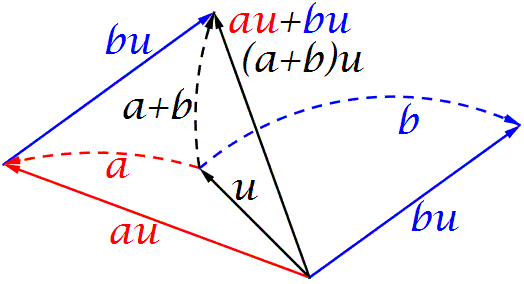
\includegraphics[width=0.5\textwidth]{imagenes/imagenes01/T01IM01.png}
		%\caption{Los dos problemas clásicos del cálculo: trazado de tangentes y áreas bajo curvas.}
	%\end{figure}
		



%\rotatebox{180}{\leftline{\textcolor{gris}{tararí}}}.

\chapter{Sistemas de ecuaciones lineales: teorema de Rouché}	
\chaptermark{S.E.L.: th. Rouché}	\label{SEL}

	
\section{Rango de una matriz}\label{rangos}

\begin{defi}.



Se dice que una matriz $M\in \mathcal M_{m \times n}(\mathbb R)$ es una \colorbox{LightYellow}{\textbf{`matriz escalonada'}}:

\noindent  --- por filas, si:

\hspace{3mm} 1.	Todas las filas de $M$ (si las hay) cuyos elementos son todos nulos aparecen en la parte inferior de la matriz. 

\hspace{3mm} 2.	El primer número no nulo (comenzando por la izquierda) en cualquier fila no nula de $M$ recibe el nombre de pivote de esa fila. 

\hspace{3mm} 3.	Cada fila de $M$ (exceptuando, por lo general, a la primera) comienza con una sucesión de ceros, de manera que siempre contiene (al menos) un cero más que la fila anterior. En otras palabras, el pivote en cualquier fila está a la derecha del pivote de la fila anterior. 

\noindent  --- por columnas, si:

\hspace{3mm} 1.	Todas las columnas de $M$ (si las hay) cuyos elementos son todos nulos aparecen a la derecha de la matriz. 

\hspace{3mm} 2.	El primer número no nulo (comenzando por arriba) en cualquier columna no nula de $M$ recibe el nombre de pivote de esa fila. 

\hspace{3mm} 3.	Cada columna de $M$ (exceptuando, por lo general, a la primera) comienza con una sucesión de ceros, de manera que siempre contiene (al menos) un cero más que la columna anterior. En otras palabras, el pivote en cualquier columna está más abajo que el pivote de la fila anterior. 
\end{defi}


\begin{ejem}.

Son matrices escalonadas: $\left( \begin{matrix} 1&2&5\\0&1&1\\0&0&1  \end{matrix} \right); \qquad \left( \begin{matrix} 1&3&2&1\\0&1&7&8\\0&0&1&3\\0&0&0&3 \end{matrix} \right)$

No lo son: $\left( \begin{matrix} \colorbox{yellow}{0}&\colorbox{yellow}{0}&5\\ \colorbox{yellow}{0}&3&7\\ \colorbox{yellow}{0}&\colorbox{yellow}{0}&4  \end{matrix} \right); \qquad \left( \begin{matrix}  1&3&2&1\\\colorbox{yellow}{0}&4&7&8\\\colorbox{yellow}{0}&\colorbox{yellow}{0}&\colorbox{yellow}{0}&3\\ \colorbox{yellow}{0}&\colorbox{yellow}{0}&5&4  \end{matrix} \right)$
	
\end{ejem}

\begin{defi}.

\colorbox{LightYellow}{Se llama \textbf{`Rango'} de una matriz $M$, $\; rg(M)\;$, al número de filas}

 \colorbox{LightYellow}{(columnas) no-nulas que quedan en la matriz escalonada $M_e$.}

%\fcolorbox{frame color}{box background color}{...}	
\end{defi}

Este número, por filas o columnas, coincide y corresponde al `número de filas (columnas) \emph{Linealmente Independientes}' que tiene la matriz. Este importante concepto lo estudiaremos en el próximo capítulo de `Espacios Vectoriales'.

Para, dada una matriz $M_{m \times n}$, obtener su rango, $\; rg(M) \;$, veremos dos métodos:

\hspace{3mm} ----- El \textbf{método de Gauss} de la matriz escalonada.

\hspace{3mm} ----- El \textbf{método de los orlados} (por adjuntos).

%$\left( \begin{matrix}   \end{matrix} \right)$
\subsection{Rango por Gauss} \label{escalonado}


Para, a partir de una matriz cualquiera $M$ obtener una matriz escalonada $M_e$ se usan transformaciones elementales de Gauss en que se puede cambiar el orden tanto de filas como de columnas (estrategia del pivote). En la práctica, en vez de llevar las filas de ceros al final, las podemos tachar.

Observación: Generalmente, cuando se utilizan operaciones elementales se pueden obtener diferentes matrices escalonadas por filas equivalentes a la de partida. Es decir, no existe una única matriz escalonada por filas asociada a una matriz A. 
%$\left( \begin{matrix}   \end{matrix} \right)$

\begin{ejem}
Calcula el rango de  $M	= \left( \begin{matrix} 1&2&0&3&4\\0&0&0&2&3\\1&2&0&5&7\\0&0&0&0&1  \end{matrix} \right) \to M_e$

$Me \to [F3\to F3-F1] \to \left( \begin{matrix} 1&2&0&3&4\\0&0&0&2&3\\0&0&0&2&3\\0&0&0&0&1  \end{matrix} \right) \to [F3\to F3-F2]  \to   \left( \begin{matrix} 1&2&0&3&4\\0&0&0&2&3\\ \text{\textst{ 0 }}&\text{\textst{ 0 }}&\text{\textst{ 0 }}&\text{\textst{ 0 }}&\text{\textst{ 0 }} \\0&0&0&0&1  \end{matrix} \right) \; \Rightarrow \; \;  \boldsymbol{ rg(M)=3 }$ 
\end{ejem}


\underline{Observación}: muchos textos dicen que calcular un rango por Gauss consiste en triangularizar la matriz de modo que por debajo de la diagonal principal todos los elementos sean cero. Entonces, prescindiendo de las trivialidades (filas de cero), el número de filas que quedan es el rango de la matriz. Esto es FALSO, hay que llegar a una MATRIZ ESCALONADA, no solo TRIANGULAR. Véase el siguiente ejemplo:

\begin{ejem}

$\left| \begin{matrix}  1&2&0&3&4\\0&0&0&2&3\\0&0&0&2&3\\0&0&0&0&1 \end{matrix} \right| \Rightarrow rango \; 4$. Falso, esta matriz es triangular pero no está escalonada, la fila $3$ no tiene más ceros a la izquierda que la dos (si nos damos cuenta, es la misma y podemos prescindir de ella). Al seguir buscando ceros en $F3\to F3-F2$ obtenemos una trivialidad:

$\left| \begin{matrix}  1&2&0&3&4\\0&0&0&2&3\\ \text{\textst{ 0 }}&\text{\textst{ 0 }}&\text{\textst{ 0 }}&\text{\textst{ 0 }}&\text{\textst{ 0 }}  \\0&0&0&0&1 \end{matrix} \right| \Rightarrow rango \; 3$.

	
\end{ejem}


\subsection{Rango por adjuntos. Método de los orlados.}

\begin{defi}.

Si en una matriz de orden $m \times n$ tomamos $k$ filas y $k$ columnas y formamos  un determinante de orden $k$ se le llama menor de orden $k$, $\; M_k$.

Si a este $M_k$ se le añaden una fila y una columna cualesquiera de $M$ se obtiene un menor de orden $k+1$  que se llama \textbf{menor orlado}.

Definimos el rango de la matriz $M$ como   \colorbox{LightYellow}{$rg(M)=\; $el orden del mayor}  \colorbox{LightYellow}{ menor no-nulo} obtenido de $M$

Dada $M_{m \times n}$ siempre se verificará que  \colorbox{LightYellow}{$\boxed{ \; rg(M) \le min\{ m,\; n \} \; }$}. Para encontrar el rango de una matriz bastará con encontrar un $M_k \neq 0$ tal que todos los $M_{k+1}$ orlados a través de él sean cero. Para esto usaremos el:

\end{defi}

\textbf{Método de los Orlados}: partimos de un menor no nulo y vamos orlando con las filas y columnas restantes hasta encontrar el máximo menor no nulo de la matriz. Su orden es el rango. 

En la práctica:

----- Se prescinde de todas las líneas formadas por ceros, ya que al añadir filas o columnas de ceros a un determinante, éste resulta nulo.

----- Si a simple vista se descubre alguna línea que sea igual o proporcional a otras, se prescinde de ella.


\begin{ejem} Calcula el rango de  $M	= \left( \begin{matrix} 1&2&0&3&4\\0&0&0&2&3\\1&2&0&5&7\\0&0&0&0&1  \end{matrix} \right)$

Rápidamente encontramos en $M$ un menor de orden $2$ distinto de cero:



$M_2=\left| \begin{matrix} 3&4\\2&3  \end{matrix} \right|=9-8=1\neq 0$. Luego $rg(M)\ge 2$, veamos si puede ser $3$. Para ello vamos a `orlar' el menor anterior con filas y columnas para obtener menores de orden $3$ hasta que encontremos uno de ellos distinto de cero ($rg(M)\ge 3$) o comprobemos que todos ellos son cero ($rg(M)=2$). \textcolor{gris}{\emph{Obsérvese que a partir de nuestro menor de orden $2$ distinto de cero $(M_2$) podemos encontrar hasta $6$ menores de orden $3$, orlando con F3C3, F4C3, F3C2, F4C2, F3C1 y F4C1}}

Podemos orlar a $M_2$ con elementos de la $C3$, pero al ser todo ceros, seguro que el menor de orden $3$ que busquemos resulta nulo, así que empecemos orlando a $M_2$ con elementos de $C2$, podemos añadir la $F3$ o la $F4$, empecemos con $M_2,\; C3,\; F3$:

$\left| \begin{matrix} 2 & \boxed{3} & \boxed{4} \\ 0 & \boxed{2} & \boxed{3} \\ 2 & 5 & 7  \end{matrix} \right| = 28+0+18-(16+30+0)=46-46=0$

Veamos lo que ocurre al orlar con la $F4$, es decir:  $M_2,\; C3,\; F4$:

$M_3=\left| \begin{matrix} 2 & \boxed{3} & \boxed{4} \\ 0 & \boxed{2} & \boxed{3} \\ 0 & 0 & 1  \end{matrix} \right| = 2\; (-1)^{1+1}\cdot 1=2\neq 0 \Rightarrow  rg(M)\ge 3$

A partir ahora de este $M_3 \neq 0$, continuamos orlando. Ahora solo podemos añadir la $C1$ y $F3$ para obtener:

$\left| \begin{matrix} 1& \boxed{2} & \boxed{3} & \boxed{4} \\ 0 & \boxed{0} & \boxed{2} & \boxed{3} \\ 1 & 2 & 5 & 7 \\ 0 & \boxed{0} & \boxed{0} & \boxed{1}  \end{matrix} \right| = \; [C2=2\cdot C1] \; = 0 \Rightarrow rg(M) \neq 4$

Conclusión: el rango de $M$ es: $\quad \boldsymbol{rg(M)=3}$ 

\emph{\textcolor{gris}{En el próximo tema diremos que en $M$ hay $3$ filas independientes, $F1, F2, F4$ o $3$ columnas independientes $C2, C3, C4$. Podremos prescindir de $F3$, pues es `combinación lineal de las demás' o de la $C1$, por ser `combinación lineal' de  $C2, C3, C4$}}
	
\end{ejem}



Resumiendo:

\textbf{Cálculo del rango de una matriz $A$ mediante determinantes (orlando menores)}

1) Si la matriz es nula, su rango es $0$ y hemos terminado. En caso contrario, seguimos.

2) Buscamos un menor fácil de orden $2$ no nulo: $M$. Si esto no es posible, el $rg(A)=1$ y hemos terminado.

3) Elegimos una fila de $A$ que no esté en $M$ .Orlamos $M$ : completamos un nuevo menor con elementos de dicha fila y una columna que no esté en $M$. Si dicho menor vale $0$, elegimos otra columna, y así hasta completar todas las columnas de $A$, siempre con dicha fila.

\hspace{5mm} a) Si todos esos menores valen $0$, la fila elegida es `combinación lineal' de las filas que están en $M$, y puede ignorarse a efectos del cálculo del rango. En ese caso, repetimos el paso $2$ con otra fila, y así hasta completar todas las filas de $A$.

\hspace{5mm}  b) Si alguno de esos menores es no nulo, el rango de $A$ es el orden de dicho menor, como mínimo. Llamamos $M$ a dicho nuevo menor no nulo y repetimos el
paso $3$ con otra fila.

4) El rango de $A$ será el orden del máximo menor no nulo $M$ encontrado con este procedimiento. Las filas y columnas de $A$ que figuran en $M$ son `linealmente independientes'. A dicho menor $M$ se le llama \textbf{menor principal}. Las filas y columnas que no están en $M$ son `combinación lineal' de las que sí aparecen en $M$. (más en el próximo tema de espacios vectoriales).

\vspace{20mm}

\section{Método de Cramer}

\begin{defi}
Se dice que un SEL es de Cramer si tiene el mismo número de ecuaciones que de incógnitas y, escrito matricialmente, el determinante de la matriz de los coeficientes es distinto de cero.	
\end{defi}


Un sistema de ecuaciones lineales `cuadrado', es decir, con tantas ecuaciones como incógnitas, se puede interpretar como una ecuación matricial:

$\begin{cases} a_{11}x_1+a_{12}x_2 + \cdots + a_{1n}x_n &=b_1 \\
a_{12}x_1+a_{22}x_2 + \cdots + a_{2n}x_n &=b_2 \\
\cdots + \cdots + \cdots + \cdots + \cdots  &=\cdots \\
a_{n1}x_1+a_{n2}x_2+\cdots +a_{nn}x_n &=b_n  \end{cases} \quad \Leftrightarrow \quad \boxed{\; AX=B\; \; }$	,

donde:
$A=\left( \begin{matrix}  a_{11}&a_{12}& \cdots &a_{1n} \\
a_{12} &a_{22} &\cdots &a_{2n} \\
\cdots & \cdots & \cdots & \cdots  \\
a_{n1} &a_{n2} &\cdots &a_{nn}    \end{matrix} \right); \; X=\left( \begin{matrix} x_1\\x_2\\ \vdots \\x_n \end{matrix} \right); \; B=\left( \begin{matrix} b_1\\b_2\\ \vdots \\b_n \end{matrix} \right)$

$A$ es la matriz de los coeficientes, $X$ la de incógnitas y $B$ la de términos independientes.

El que este \colorbox{LightYellow}{SEL-cuadrado} sea de \colorbox{LightYellow}{Cramer} implica que \colorbox{LightYellow}{$\boldsymbol{ \; |A|\neq 0\; }$} $\; \to \exists A^{-1} \to \boldsymbol{ X=A^{-1}B }$

Recordando que la matriz adjunta de $A$ está formada por los elemento $A_{ij}$ y que la inversa es uno partido por el determinante de la matriz adjunta de la matriz \emph{traspuesta}, esta ecuación se puede escribir como:

\vspace{3mm}

\centerline{$\left( \begin{matrix} x_1\\x_2\\ \vdots \\ \boldsymbol{ x_i} \\ \vdots \\x_n  \end{matrix} \right) =
\dfrac 1 {|A|}\;
\left( \begin{matrix} A_{11}&A_{21}& \cdots &A_{n1}\\
A_{12}&A_{22}& \cdots & A_{n2}\\
\vdots & \vdots & \ddots & \vdots \\
\boldsymbol{A_{1i}}&\boldsymbol{A_{2i}}& \cdots & \boldsymbol{A_{ni}} \\
\vdots & \vdots & \ddots & \vdots \\
A_{1n}&A_{2n}& \cdots & A_{nn}  \end{matrix} \right) 
\cdot \boldsymbol{\left( \begin{matrix} b_1\\b_2\\ \vdots \\ b_i \\ \vdots \\ b_n  \end{matrix} \right)}$}

\justify 

\vspace{2mm}
\centerline{$x_i=\dfrac 1 {|A|}\; \left( b_1A_{1i}+b_2A_{2i}+\cdots +b_nA_{ni}  \right) = \to $}

\vspace{2mm}
que es el desarrollo del determinante de la matriz $A$ en que se ha sustituido la columna-$i$ de coeficientes por la de términos independientes ($b_i$) y se ha desarrollado por adjuntos de Laplace de la columna-$i$:

\vspace{2mm}
\centerline{$\to = \dfrac 1 {|A|}\; \left| \begin{matrix} 
a_{11}& a_{12}& \cdots & \textcolor{red}{b_1} & \cdots & a_{1n} \\
a_{21}& a_{22}& \cdots & \textcolor{red}{b_2} & \cdots & a_{2n} \\
\vdots & \vdots & \ddots & \vdots & \ddots & \vdots \\
a_{n1}& a_{n2}& \cdots & \textcolor{red}{b_n} & \cdots & a_{nn} \\
 \end{matrix} \right| $}
 
 Luego, resolver un sistema de Cramer (cuadrado con $|A|\neq 0$) consiste en calcular $(n+1)$ determinantes, uno para cada incógnita más el de los coeficientes y el resultado de cualquier incógnita consiste en calcular el determinante de $A$ en que se ha sustituido la columna correspondiente a la incógnita a calcular por la columna de términos independientes y dividirlo por el determinante de $A$.
 
\noindent Cramer $\begin{cases} n \times n \\ |A|\neq 0 \end{cases} \Rightarrow \;$ \colorbox{LightYellow}{$  \boxed{\; \textcolor{red}{x_i}= \dfrac 1 {|A|}\; \left| \begin{matrix} 
a_{11}& a_{12}& \cdots & \textcolor{red}{b_1} & \cdots & a_{1n} \\
a_{21}& a_{22}& \cdots & \textcolor{red}{b_2} & \cdots & a_{2n} \\
\vdots & \vdots & \ddots & \vdots & \ddots & \vdots \\
a_{n1}& a_{n2}& \cdots & \textcolor{red}{b_n} & \cdots & a_{nn} \\
 \end{matrix} \right|\;}$}
 
 \begin{ejem}
 Resuelve por Cramer, si es posible: $\begin{cases}
x+2y-z&=-3\\x\quad \quad +\; z&=1\\2x-y+2z&=4	
\end{cases}$

Tenemos un sistema cuadrado: 3 ecuaciones con 3 incógnitas, con $|A|=\left| \begin{matrix} 1&2&-1\\1&0&1\\2&-1&2   \end{matrix} \right| = 0+1+4-(0-1+4)=5-3= \textcolor{blue}{\boldsymbol{2}} \neq 0 \to \;$ sí es resoluble por Cramer:

$\boldsymbol{x}=\dfrac 1 {\textcolor{blue}{\boldsymbol{2}}} \; \left| \begin{matrix} \textcolor{red}{3}&2&-1\\ \textcolor{red}{-1}&0&1\\ \textcolor{red}{4}&-1&2   \end{matrix} \right| = \dfrac 1 4 \; [0+1+8 -(0-3+4 )] \dfrac 1 2 (9-7)=\boldsymbol{1}  $

$\boldsymbol{y}=\dfrac 1 {\textcolor{blue}{\boldsymbol{2}}} \; \left| \begin{matrix} 1&\textcolor{red}{3}&-1\\1&\textcolor{red}{-1}&1\\2&\textcolor{red}{4}&2   \end{matrix} \right| = \dfrac 1 4 \;[2-4-6 -(-2+4-6 )]=\dfrac 1 2 [-8-(-4)]  = \boldsymbol{2} $

$\boldsymbol{z}=\dfrac 1 {\textcolor{blue}{\boldsymbol{2}}} \; \left| \begin{matrix} 1&2&\textcolor{red}{3}\\1&0&\textcolor{red}{-1}\\2&-1&\textcolor{red}{4}   \end{matrix} \right| = \dfrac 1 4 \;[0+3+4 -(0-1+8 )] =\dfrac 1 2 (7-7)  =\boldsymbol{ 0} $

SCD

 \end{ejem}

\emph{Ventajas e inconvenientes} del método de Cramer frente al método de Gauss:

\begin{itemize}
\item Si el sistema es de Cramer (que no lo son todos los SEL), Cramer nos permite, sin resolver todo el sistema, conocer el valor de cualquier incógnita del sistema sin más que calcular un cociente de determinantes.

\item Pero el SEL puede no ser de Cramer y Gauss es válido para cualquier tipo de SEL.
\end{itemize}


%$\left| \begin{matrix}   \end{matrix} \right|$
%$\left( \begin{matrix}   \end{matrix} \right)$

%$\left( \begin{matrix}   \end{matrix} \right)$
\section{Teorema de Rouché-Frobenius}


Consideremos un SEL cualquiera, de $m$ ecuaciones lineales con $n$ incógnitas:

\centerline {$\begin{cases} a_{11}x_1+a_{12}x_2 + \cdots + a_{1n}x_n &=b_1 \\
a_{12}x_1+a_{22}x_2 + \cdots + a_{2n}x_n &=b_2 \\
\cdots  \cdots  \cdots  \cdots  \cdots  \cdots \cdots  \cdots  \cdots  &= \cdots \\
a_{m1}x_1+a_{m2}x_2+\cdots +a_{mn}x_n &=b_m  \end{cases} $	,}

\justify
Llamamos matrices $A$ de los coeficientes y $A^*$ matriz ampliada a las matrices:



$A=\left( \begin{matrix}  a_{11}&a_{12}& \cdots &a_{1n} \\
a_{12} &a_{22} &\cdots &a_{2n} \\
\cdots & \cdots & \cdots & \cdots  \\
a_{m1} &a_{m2} &\cdots &a_{mn}    \end{matrix} \right); \; \; A^*=
\left( \begin{matrix}  a_{11}&a_{12}& \cdots &a_{1n} \\
a_{12} &a_{22} &\cdots &a_{2n} \\
\cdots & \cdots & \cdots & \cdots  \\
a_{m1} &a_{m2} &\cdots &a_{mn}    \end{matrix} \right|
\left. \begin{matrix} b_1\\b_2\\ \vdots \\ b_m \end{matrix} \right)$

Escrito en una sola matriz, por delante, hasta la barra vertical, tenemos a la matriz $A$, por detrás, sin la barra, la matriz $A^*$.

\begin{myblock}{Matriz de coeficientes y ampliada}

\centerline{$\; A=
\left( \begin{matrix}  a_{11}&a_{12}& \cdots &a_{1n} \\
a_{12} &a_{22} &\cdots &a_{2n} \\
\cdots & \cdots & \cdots & \cdots  \\
a_{m1} &a_{m2} &\cdots &a_{mn}    \end{matrix} \right|
\left. \begin{matrix} b_1\\b_2\\ \vdots \\ b_m \end{matrix} \right) \leftarrow A^*\; $}
\end{myblock}

\begin{teor}{Teorema de Rouché-Frobenius} \textcolor{gris}{(sin demostración)}

\vspace{4mm}

\centerline{\colorbox{LightYellow}{Un SEL es COMPATIBLE si $\boxed{\; rg(A)=rg(A^*)\; }$}}

\vspace{2mm}

-----  \colorbox{LightYellow}{si $\; rg(A)=rg(A^*) =$ número de incógnitas $\longrightarrow$ \textbf{SCD}}

-----  \colorbox{LightYellow}{si $\; rg(A)=rg(A^*) <$ número de incógnitas $\longrightarrow $ \textbf{SCI}}

----- \colorbox{LightYellow}{Obviamente, si $\; rg(A) \neq rg(A^*)$ $\longrightarrow $ \textbf{SI}}

En el caso $\; rg(A)=rg(A^*) <$ número de incógnitas , se llaman \textbf{ecuaciones principales del sistema} a las que forman el menor que dicta en rango, las otras ecuaciones se pueden eliminar y se llaman \textbf{incógnitas principales del sistema} a las que forman el menor que dicta el rango, las restantes se parametrizan, es decir, se les asignan valores reales cualesquiera, parámetros (letras griegas) y se pasan al segundo miembro quedando ahora un SEL cuadrado con determinante de los coeficientes principales distinto de cero con lo que el problema se puede resolver por Cramer (o por Gauss).
	
\end{teor}

\subsection{Aplicación a sistemas homogéneos}

Todo SEL de $m$ ecuaciones con $n$ incógnitas homogéneo ($b_1=b_2= \cdots = b_m=0$) admite siempre la  \textbf{solución trivial} $x_1=x_2= \cdots = x_n=0$, por lo que son siempre COMPATIBLES. 

Esto es evidente a la luz del teorema de Rouché puesto que si $A$ tiene rango $k$, $A^*$ también tendrá rango $k$ ya que $A^*$ no consiste más que en añadir a $A$ una columna de ceros y, obviamente, no altera el rango.

Según el teorema de Rouché, 

\hspace{2mm} ----- si $k=rg(A)=n=$número de incógnitas $\to $ el SEL es SCD, solución única: `la trivial' $(0,0, \cdots , 0)$

\hspace{2mm} -----  si $k=rg(A)<n=$número de incógnitas $\to $ el SEL es SCI,  infinitas soluciones (habrá que parametrizar) , entre ellas estará `la trivial' $(0,0, \cdots , 0)$


\section{Discusión de sistemas}

En ocasiones se nos presentará resolver SEL dependientes de uno o varios parámetros. Para ello usaremos el teorema de Rouché para determinar los rangos de $A$ y $A^*$ analizando todos los posibles casos que puedan presentarse en función del valor que tomen los parámetros del sistema (esto es lo que se llama `discusión de SEL') y resolviendo en los casos de compatibilidad.

\underline{Observación importante:} Para analizar el rango de una matriz usaremos el método ascendente de los orlados ---a no ser que nos pidan usar el método de Gauss--- (ver si la matriz tiene rango $1$; si lo tiene, ver si puede tener rango $2$; si es así, ver si el rango es $3$; etc). Pero si la matriz $A$ o $A^*$ son cuadradas procederemos al revés, viendo si pueden tener rango máximo, estudiaremos su determinante.

En el siguiente apartado de ejercicios resueltos veremos muchos ejemplos de discusión y resolución de SEL con el teorema de Rouché.
%$\text{\textst{ 0 }}$

% \text{\textst{ 0 }}&\text{\textst{ 0 }}&\text{\textst{ 0 }}&\text{\textst{ 0 }}&\text{\textst{ 0 }}

\section{Eliminación de parámetros $\divideontimes$}

\justify

\emph{La \textbf{eliminación de parámetros} es el proceso inverso a resolver un sistema de ecuaciones que sea compatible
indeterminado} (los sistemas que tienen infinitas soluciones  que  dependen  de uno o más parámetros), es decir,  pasar de las soluciones paramétricas de un SCI a las ecuaciones normales (implícitas, sin parámetros) que da lugar a esta solución. Así pues, lo que haremos es, dada la solución con parámetros encontrar el sistema de ecuaciones (o uno equivalente) que da lugar a esa solución.

En general, las soluciones de un sistema de ecuaciones expresadas en parámetros es (solución de un SEL que sea SCI):

\begin{equation*}
	\begin{cases}
	x_1=k_1+c_{11}t_1+c_{12}t_2+\cdots +c_{1p}t_p \\
	x_2=k_2+c_{21}t_1+c_{22}t_2+\cdots +c_{2p}t_p \\
	\cdots  \cdots \cdots \cdots \cdots \cdots \cdots \cdots \cdots \cdots \cdots\\
	x_n=k_n+c_{n1}t_1+c_{n2}t_2+ \cdots + c_{np}t_p
	\end{cases}
\end{equation*} 

\noindent que son las $n$-soluciones de las $n$-incógnitas dependientes de $p$-parámetros obtenidas del SEL de $m$-ecuaciones con $n$-incógnitas. Se trata de encontrar ese SEL, o uno equivalente, que proporcione esta misma solución.

\underline{Procedimiento para la eliminación de parámetros}:

1. Reescribir el sistema considerando los parámetros como incógnitas y las incógnitas como términos independientes:

\begin{equation*}
	\begin{cases}
	c_{11}t_1+c_{12}t_2+\cdots +c_{1p}t_p=x_1-k_1 \\
	c_{21}t_1+c_{22}t_2+\cdots +c_{2p}t_p=x_2-k_2 \\
	\cdots  \cdots \cdots \cdots \cdots \cdots \cdots \cdots \cdots \cdots \cdots\\
	c_{n1}t_1+c_{n2}t_2+ \cdots + c_{np}t_p=x_n-k_n
	\end{cases}
\end{equation*}

2. Este nuevo sistema ha de ser, también, \emph{\textbf{compatible}}, luego: 

\vspace{2mm}
\centerline{\colorbox{LightYellow}{$\; rg(A)=rg(A^*) \;$},} 

\noindent siendo $A$ y $A^*$ las  matrices de coeficientes y asociada a este nuevo sistema. Al exigir que se cumpla esta condición aparecen las relaciones entre las incógnitas que darán lugar al SEL buscado.

3. El número de ecuaciones obtenidas corresponde con el número de condiciones que debe haber entre las incógnitas $x_1,x_2,\cdots ,x_n$ (\textcolor{gris}{\emph{ligaduras}}) para que el sistema tenga solución. Se cumplirá que: (n=número de incógnitas)

\begin{equation*}
\colorbox{LightYellow}{\boxed{\text{ Número de ecuaciones } = n-rg(A)\; }}	
\end{equation*}

En en apartado `ejercicios resueltos' veremos ejemplos de resolución de eliminación de parámetros.


\section{Ejercicios}

\subsection{Ejercicios resueltos}

\begin{ejre} Estudia el rango de las siguientes matrices por el método de Gauss y por el método de los orlados.

$A=\left( \begin{matrix} 1&3&-2\\5&1&2  \end{matrix} \right); \quad
B=\left( \begin{matrix} -1&2&1\\2&11&5\\2&-1&3  \end{matrix} \right); \quad
C=\left( \begin{matrix}  1&2&-1&3\\3&7&0&11\\-4&-6&10&-3 \end{matrix} \right)$

$D=\left( \begin{matrix} 3&10&-1 \\ 1&3&-1 \\ -1&-1&8\\2&10&7  \end{matrix} \right); \quad 
E=\left( \begin{matrix} 2&-1&0&0\\0&0&2&-1\\0&2&-1&0\\2&0&-1&0  \end{matrix} \right)$
\end{ejre}
\begin{proofw}\renewcommand{\qedsymbol}{$\diamond$}

%\rule{45mm}{0.2pt}

------ \underline{Método de Gauss}
	
\noindent  * rango de $A \to   \left( \begin{matrix} 1&3&-2\\5&1&2  \end{matrix} \right) \to  [F2\to F2-5F1 \to \left( \begin{matrix} 1&3&-2\\0&-14&12  \end{matrix} \right) \Rightarrow \boldsymbol{rg(A)=2}$

\noindent  * rango de $B \to \left( \begin{matrix} -1&2&1\\2&11&5\\2&-1&3  \end{matrix} \right)  \to \left[ \begin{matrix}  F2\to F2+2F1 \\ F3\to F3+2F1 \end{matrix} \right] \to \left( \begin{matrix} -1&2&1\\0&15&7\\0&3&5  \end{matrix} \right)  \to [F3 \to 5F3-F2] \to \left( \begin{matrix} -1&2&1\\0&15&7\\0&0&18  \end{matrix} \right) \Rightarrow \boldsymbol{rg(B)=3}$

\noindent  * rango de $C \to \left( \begin{matrix}  1&2&-1&3\\3&7&0&11\\-4&-6&10&-3 \end{matrix} \right) \to   [C3 \leftrightarrow C1 ] \to \left( \begin{matrix}  -1&2&1&3\\0&7&3&11\\10&-6&4&-3 \end{matrix} \right) \to [F3 \to F3+10F1]\to \left( \begin{matrix}  -1&2&1&3\\0&7&3&11\\0&14&14&27 \end{matrix} \right) \to [F3 \to F3-2F2] \to \left( \begin{matrix}  -1&2&1&3\\0&7&3&11\\0&0&8&5 \end{matrix} \right) \Rightarrow \boldsymbol{rg(C)=3}$

\noindent  * rango de $D \to  \left( \begin{matrix} 3&10&-1 \\ 1&3&-1 \\ -1&-1&8\\2&10&7  \end{matrix} \right) [F1 \leftrightarrow F2 ] \to  \left( \begin{matrix} 1&3&-1 \\ 3&10&-1 \\  -1&-1&8\\2&10&7  \end{matrix} \right) \to \begin{cases} F2\to F2-3F1 \\ F3\to F3+F1  \\ F4\to  F4-2F1\end{cases} \to   \quad 
\left( \begin{matrix} 1&3&-1 \\ 0&1&2 \\  0&2&7\\0&4&9  \end{matrix} \right) \to \quad \begin{cases} F3\to F3-2F2 \\ F4 \to F4-4F2  \end{cases} \to 
\left( \begin{matrix} 1&3&-1 \\ 0&1&2 \\  0&0&3\\0&0&1  \end{matrix} \right) \to [F4\to 3F4-F3] \to  \left( \begin{matrix} 1&3&-1 \\ 0&1&2 \\  0&0&3\\ \text{\textst{ 0 }}&\text{\textst{ 0 }}&\text{\textst{ 0 }} \end{matrix} \right) \Rightarrow \boldsymbol{rg(D)=3}$


\noindent  * rango de $E \to \quad \left( \begin{matrix} 2&-1&0&0\\0&0&2&-1\\0&2&-1&0\\2&0&-1&0  \end{matrix} \right) \quad \to \quad   [F4 \to F4-F1] \quad \to \quad \left( \begin{matrix} 2&-1&0&0\\0&0&2&-1\\0&2&-1&0\\0&1&-1&0  \end{matrix} \right)  \to [F2 \leftrightarrow F4  ] \to \left( \begin{matrix} 2&-1&0&0\\0&1&-1&0\\0&2&-1&0\\0&0&2&-1  \end{matrix} \right) \to [F3 \to F3-2F2] \to \left( \begin{matrix} 2&-1&0&0\\0&1&-1&0\\0&0&1&0\\0&0&2&-1  \end{matrix} \right) \to [F4 \leftrightarrow F3 ] \to \left( \begin{matrix} 2&-1&0&0\\0&1&-1&0\\0&0&2&-1\\0&0&1&0  \end{matrix} \right) \to [F4 \to 2F4-F3] \to \left( \begin{matrix} 2&-1&0&0\\0&1&-1&0\\0&0&2&-1\\0&0&0&1  \end{matrix} \right) \to \Rightarrow \boldsymbol{rg(E)=4}$

\vspace{4mm}
------ \underline{Método de los orlados}

\noindent  * rango de $A \to   \left( \begin{matrix} \boxed{1}&\boxed{3}&-2\\\boxed{5}&\boxed{1}&2  \end{matrix} \right) \to \left( \begin{matrix} 1&3\\5&1  \end{matrix} \right)=1-15=-14\neq 0 \Rightarrow rg(A)\ge 2\;$ Como en $A$ hay una columna más pero no hay más filas, el rango no puede ser $3$, por lo que $\boldsymbol{ rg(A)=2}$


\noindent  * rango de $B \to \left( \begin{matrix} -1&2&1\\2&11&5\\2&-1&3  \end{matrix} \right)$; $B$ es cuadrada y nos preguntamos si tendrá rango máximo $3 \to \left| \begin{matrix} -1&2&1\\2&11&5\\2&-1&3  \end{matrix} \right|=-33-2+20-(22+5+12)=-15-39=-54\neq 0 \Rightarrow \boldsymbol{rg(B)=3}$


\noindent  * rango de $C \to \left( \begin{matrix}  \boxed{1}&\boxed{2}&-1&3\\\boxed{3}&\boxed{7}&0&11\\-4&-6&10&-3 \end{matrix} \right) \to $
$\left| \begin{matrix} 1&2\\3&7 \end{matrix} \right|=7-6=1\neq 0 \to rg(C)\ge 2\;$ 
Veamos si puede ser tres, a partir del $M_2$ marcado con cuadros en $C$, podemos orlar con $C2 y F3$ y con $C3 y F3$ a ver si encontramos un $M_3 \neq 0$ que asegure que el rango es $3$, en caso contrario (ambos determinantes fuesen cero), el rango de C se quedaría en $2$.

\noindent $\left| \begin{matrix} \boxed{1}&\boxed{2}&-1\\ \boxed{3}&\boxed{7}&0 \\-4&-6&10 \end{matrix} \right|=70+18+0-(28+0+60)=0$

\noindent $\left| \begin{matrix} \boxed{1}&\boxed{2}&3\\ \boxed{3}&\boxed{7}&11 \\-4&-6&-3 \end{matrix} \right|= -21-54-88-(-84-66-18)=5\neq 0 \Rightarrow \boldsymbol{rg(C)=3}$

\noindent \textcolor{gris}{\small{Luego en C hay $3$ fila o $3$ columnas independientes: $C \to \left( \begin{matrix}  \boxed{1}&\boxed{2}&-1&\boxed{3}\\\boxed{3}&\boxed{7}&0&\boxed{11}\\-4&-6&10&\boxed{-3} \end{matrix} \right)$}\normalsize{.}}

\noindent  * rango de $D \to  \left( \begin{matrix} \boxed{3}&\boxed{10}&-1 \\ \boxed{1}&\boxed{3}&-1 \\ -1&-1&8\\2&10&7  \end{matrix} \right) \to \left| \begin{matrix} 3&10\\1&3 \end{matrix} \right|=9-10=-1\neq 0 rg(D)\ge 2$. Podemos orlar con $C3 y F3$ o con $C3 y F4$ para ver si encontramos un $M_3 \neq 0$ que asegurase que el rango es $3$ (ya que $4$ no puede ser) o, si ambos determinantes son nulos, el rango de $E$ se quedaría en $2$.

\noindent $\left| \begin{matrix} \boxed{3}&\boxed{10}&-1\\\boxed{1}&\boxed{3}&-1\\ -1&-1&8 \end{matrix} \right|= 72+1+10-(3+3+80)=83-86=-3 \neq 0 \Rightarrow \boldsymbol{rg(D)=3}$ \textcolor{gris}{(estas tres filas o tres columnas son las linealmente independientes de $D$.)}

\noindent $\left| \begin{matrix} \boxed{3}&\boxed{10}&-1\\\boxed{1}&\boxed{3}&-1\\ 2&10&7 \end{matrix} \right|= \cdots$ Es innecesario seguir calculando. \textcolor{gris}{Tampoco es necesario escribir todos los posibles orlados, basta con encontrar uno distinto de cero o, eso sí, comprobar que todos sean cero. Lo hemos hecho así, y también en el caso siguiente, por motivos meramente didácticos.}



\noindent  * rango de $E \to \quad \left( \begin{matrix} 2&\boxed{-1}&\boxed{0}&0\\0&\boxed{0}&\boxed{2}&-1\\0&2&-1&0\\2&0&-1&0  \end{matrix} \right)  \to \left| \begin{matrix} -1&0\\0&2 \end{matrix} \right|=-2-0=-2\neq 0 \to rg(E)\ge 2$ Para comprobar si el rango es tres podemos orlar este $M_2$ con filas y columnas: $C1F3; \; C1F4; \; C4F3; \; C4F4$. Hay que ir calculando determinantes hasta encontrar uno distinto de cero ($rg(E)\ge 3$) o comprobar que todos ellos son cero ($rg(E)=2$). Vamos a por ellos:

\noindent $\left| \begin{matrix} 2&\boxed{-1}&\boxed{0}\\0&\boxed{0}&\boxed{2}\\0&2&-1 \end{matrix} \right| = 2(-1)^{1+1}\; (-2+0)=-4\neq 0 \to rg(E)\ge 3$

\noindent $\left| \begin{matrix} 2&\boxed{-1}&\boxed{0}\\0&\boxed{0}&\boxed{2}\\2&0&-1 \end{matrix} \right| = $ No es necesario continuar.

\noindent $\left| \begin{matrix} \boxed{-1}&\boxed{0}&0\\ \boxed{0}&\boxed{2}&-1 \\2&-1&0 \end{matrix} \right| = $ No es necesario continuar.

\noindent $\left| \begin{matrix} \boxed{-1}&\boxed{0}&0\\ \boxed{0}&\boxed{2}&-1\\0&-1&0 \end{matrix} \right| = $ No es necesario continuar.

\noindent A parir del $M_3\neq 0$ obtenido anteriormente podemos orlar con $C4F4$:

\noindent $(*)\; \left| \begin{matrix} 2&-1&0&0\\0&0&2&-1\\0&2&-1&0\\2&0&-1&0  \end{matrix} \right| = \quad [F4\to F4-F1]\quad = \left( \begin{matrix} 2&-1&0&0\\0&0&2&-1\\0&2&-1&0\\0&1&-1&0  \end{matrix} \right)\quad = \quad 2 (-1)^{1+1} \; \left| \begin{matrix} 0&2&-1\\2&-1&0\\ 1&-1&0 \end{matrix} \right|= 2 [0-2+0-(1+0+0)]=2\cdot(-3)=-6\neq 0 \Rightarrow \boldsymbol{rg(E)=4}$

Si recuerda el/la lector/a, dijimos anteriormente que si la matriz era cuadrada convenía hacer el estudio de los rangos al revés, viendo si el rango era máximo, con lo que hubiésemos empezado calculando $|E|=)*)=-6\neq 0 \Rightarrow \boldsymbol{rg(E)=4}$ y hubiésemos acabado antes. Quede este ejercicio como recuerdo de que en matrices cuadradas conviene hacer el estudio de los rangos de modo `descendente', empezando por ver si el rango es máximo.

\end{proofw}


\begin{ejre}
	Halla el rango de las siguientes matrices en función del valor que tome el parámetro:

\noindent $A=\left( \begin{matrix} 2&-1&-3&5\\2&2&-1&\lambda\\1&1&1&6\\3&1&-4&\lambda \end{matrix} \right); \;\;   \qquad 
B=\left( \begin{matrix} 1&k\\k&9\\2&6  \end{matrix} \right); \;\;   \qquad 
C=\left( \begin{matrix} 1&1&1&k\\k&k^2&1&1\\1&1&k&1  \end{matrix} \right);$

\noindent $D=\left( \begin{matrix} 1&1&2\\-1&a&-3\\1&a+2&1\\2&0&5  \end{matrix} \right); \;  \qquad 
E=\left( \begin{matrix} m-1&1&m&1\\1&m-1&m&1\\1&1&2&m-1  \end{matrix} \right)$
\end{ejre}

\begin{proofw}\renewcommand{\qedsymbol}{$\diamond$}


------ $rg(A)\; $: Como $A$ es cuadrada $(A_4)$, veamos si tiene rango máximo ($4$):

$\left| \begin{matrix} 2&-1&-3&5\\2&2&-1&\lambda\\ \boldsymbol{1}&\boldsymbol{1}&\boldsymbol{1}&\boldsymbol{6}\\3&1&-4&\lambda \end{matrix} \right|= \to \begin{cases} C2\to C2-C1 \\ C3\to C3-C1 \\ C4\to C4-6C1   \end{cases} \to = \left| \begin{matrix} 2&-3&-5&-7\\2&0&-3&\lambda-12\\ \boldsymbol{1}&\boldsymbol{0}&\boldsymbol{0}&\boldsymbol{0}\\3&-2&-7&\lambda-18 \end{matrix} \right|= 1 (1-)^{3+1}\; \left| \begin{matrix} -3&-5&-7\\0&-3&\lambda-12\\-2&-7&\lambda-18 \end{matrix} \right| = 9(\lambda-18)+10(\lambda-12)-(-42+21(\lambda-12))=9(\lambda-18)-11(\lambda-12)+42=-2\lambda+12=0 \leftrightarrow \lambda=6$. Hemos de distinguir dos casos, $\lambda=6$ y $\lambda\neq 6$:

(1*) Si $\boldsymbol{ \lambda\neq 6} \to |A|\neq 0 \Rightarrow \boldsymbol{rg(A)=4}$

(2*)  Si $\boldsymbol{ \lambda = 6} \to $ particularicemos $A(\lambda=6)$ y estudiemos ascendentemente el rango de A, que sabemos que no puede ser $4$:

$A(6)=\left( \begin{matrix} \boxed{2}&\boxed{-1}&-3&5\\\boxed{2}&\boxed{2}&-1&\boldsymbol{6}\\1&1&1&6\\3&1&-4&\boldsymbol{6} \end{matrix} \right) $ Como $\left| \begin{matrix} 2&-1||2&2 \end{matrix} \right|=4-(-2)=6\neq 0 \to rg(A)\ge 2$. Vamos orlando. Empezamos con $F3C3\to \left| \begin{matrix} 2&-1&-3\\2&2&-1\\1&1&1 \end{matrix} \right|= 4-3+1-(-6-2-1)=2-(-9)=11\neq 0 \Rightarrow \boldsymbol{rg(A)=3}$, puesto que ya sabemos que no puede ser $4 \; (\lambda=6)$.

------ $rg(B)\; $: Como $B$ no es cuadrada, hay que hacer un estudio ascendente. \emph{¡Consejo! `Cuanto más tardes a tomar el parámetro, mejor'.}

$\left( \begin{matrix} \boldsymbol{1}&\boldsymbol{k}\\k&9\\\boldsymbol{2}&\boldsymbol{6}  \end{matrix} \right) \to \left| \begin{matrix} 1&k\\2&6 \end{matrix} \right|=6-2k=0 \leftrightarrow k=3$

Sabemos que si $\boldsymbol{k\neq 3} \to M_2\neq 0 \Rightarrow \boldsymbol{rg(B)=2}$, puesto que no puede ser $3$.

Pero, si $\boldsymbol{k=3}$, este $M_2=0$, pero hay otro. particularicemos $B(3)=\left( \begin{matrix} \boxed{1}&3\\3&9\\2&6 \end{matrix} \right) \to \left| \begin{matrix} \boxed{1}&3\\3&9 \end{matrix} \right|= 9-9=0$ Luego, con $k=3$ todos los menores de orden dos son nulos $\Rightarrow \boldsymbol{rg(B)=1}$

------ $rg(C)\; $: Como $C$ no es cuadrada, haremos el estudio ascendente:

$C=\left( \begin{matrix} 1&1&1&k\\k&k^2&\boxed{1}&\boxed{1}\\1&1&\boxed{k}&\boxed{1}  \end{matrix} \right)  $ Como no encontramos ningún $M_2\neq 0$ que no tenga parámetros, empezamos por el que vemos más sencillo (con menos parámetros): $\; \left| \begin{matrix} 1&1\\k&1 \end{matrix} \right|=1-k=0 \leftrightarrow k=1$

Tenemos pues dos casos, $k=1$ y $k\neq 1$:

(1*) si $k=1 \to C(1)=\left( \begin{matrix} 1&1&1&1\\1&1&1&1\\1&1&1&1 \end{matrix} \right) \Rightarrow $, evidentemente, $rg(C)=1$ 

(2*) si $k \neq 1 \to  M_2\neq 0 \to rg(C)\ge 2$ y orlaremos con las columnas 2 y 3 y con la fila 1 (dos posibilidades), sabiendo en todo momento que $k \neq 1 $: 

Empecemos orlando con $C1$ y $F1$: $\; \left| \begin{matrix} 1&1&k\\k&1&1\\1&k&1 \end{matrix} \right|= 1+K^3+1-(k+k+k)=k^3-3k+2=\text{ (Ruffini) }=(k-1)^2(k+2) \neq 0 \to \begin{cases} k\neq 1 \text{ ya lo es (1*) }\\ k\neq 2 \end{cases} \to $

(2*-a) Si $k\neq 1$ y $k\neq -2$ este $M_3\neq 0 \to rg(C)=3$

(2*-b) Si $k=-2 \to$ particularizamos: $C(2)=\left( \begin{matrix} 1&1&1&-2\\-2&4&\boldsymbol{1}&\boldsymbol{1}\\1&1&\boldsymbol{-2}&\boldsymbol{1} \end{matrix} \right) \to \left| \begin{matrix} 1&1&-2\\4&1&1\\1&-2&1 \end{matrix} \right| = 1+16+1-(-2-2+4)=18\neq 0 \to rg(C)=3$

Conclusión: $\begin{cases} \text{ si } \boldsymbol{k=1} \Rightarrow \boldsymbol{rg(C)=1 } \\  \text{ si } \boldsymbol{k\neq -1} \to (k=-2\; \vee \; k\neq -2) \Rightarrow \boldsymbol{rg(C)=3} \end{cases}$
	

------$rg(D)$: Al no ser $D$ cuadrada, haremos un estudio ascendente.

$\left( \begin{matrix} \boxed{1}&1& \boxed{2}\\-1&a&-3\\1&a+2&1\\ \boxed{2}&0& \boxed{5}  \end{matrix} \right) \to \left| \begin{matrix} 1&2\\2&5 \end{matrix} \right| = 5-4=1 \to M_2\neq 0 \to rg(D)\ge 2$. Podemos orlar con C2 y F2 y con C2 y F3:

$\left| \begin{matrix} 1&1&2\\-1&a&-3\\2&0&5 \end{matrix} \right|= 5a-6-(4a-5)=a-1=0 \leftrightarrow a=1 \to $ distinguiremos dos casos: $a=1$ y $a\neq 1$

(1*) Si $a\neq 1\to M_3\neq 0 \Rightarrow rg(D)=3$

(2*) Si $a=1\to $ particularizamos: $\;  D(1)=\left( \begin{matrix} \boxed{1}&1&\boxed{2}\\-1&\boldsymbol{1}&-3\\1&\boldsymbol{3}&1\\\boxed{2}&0&\boxed{5}  \end{matrix} \right) $ Podemos orlar el $M_2\neq 0$ con $F2 y C2$ que ya sabemos que dará cero, pero aún nos queda la posibilidad de orlar con $F3 y C2$:

$\left| \begin{matrix} 1&1&2\\1&3&1\\2&0&5 \end{matrix} \right|= 15+2-(12+5)=17-17=0 $, luego, si $a=1 \to rg(D)=2$

Conclusión. $\begin{cases} \text{ si } \boldsymbol{a\neq 1 \to rg(D)=3} \\ \text{ si } \boldsymbol{a=1 \to rg(D)=2}  \end{cases}$


------ $rg(E)$: $E$ no es cuadrada, estudio ascendente: 


$\left( \begin{matrix} m-1&1&m&1\\ \boxed{1}&\boxed{m-1}&m&1\\\boxed{1}&\boxed{1}&2&m-1  \end{matrix} \right) \to \left| \begin{matrix} 1&m-1\\1&1 \end{matrix} \right|= 1-(m-1)=2-m=0 \leftrightarrow m=2   $ Distinguiremos dos casos, $m=2$ y $m\neq 2$

(1*) si $m=2\to E(2)=\left( \begin{matrix} 1&1&2&1\\1&1&2&1\\1&1&2&1\end{matrix} \right) \to $ tres filas iguales $\to rg(E)=1$

(2*) si $m\neq 2 \to rg(E)\ge 2$ (puede ser hasta tres), hay dos menores de orden tres, orlando con $F1C4$ y con $F1C3$, probemos con la primera posibilidad:

$\left| \begin{matrix} m-1&1&1\\1&m-1&1\\1&1&m-1 \end{matrix} \right|=(m-1)^3+1+1-3(m-1)=m^3-3m^2+4=0 \leftrightarrow \begin{cases}  m=2 \text{ \footnotesize{(no considerado)}\normalsize{.}} \\ m=-1 \end{cases}$ Tenemos ahora dos sub-casos: $m\neq 2 \; \wedge \; m\neq -1$ y $m\neq 2 \; \wedge \; m= -1$, analicémoslos:

(2*-a) $m\neq 2 \; \wedge \; m\neq -1$, el $M_3$ anterior es distinto de cero, por lo que $rg(E)=3$, no puede ser cuatro.

(2*-b) $m\neq 2 \; \wedge \; m=-1$, particularizamos el $M_3$ anterior y tenemos: $\left| \begin{matrix} -2&1&1\\1&-2&1\\1&1&-2 \end{matrix} \right|=-8+1+1-(-2-2-2)=-6-(-6)=0 \to rg(E)=2$.

Conclusión. $\begin{cases} 
\boldsymbol{m=2\Rightarrow rg(E)=1} \\ 
\boldsymbol{m=-1 \Rightarrow rg(E)=2} \\ 
\boldsymbol{m\neq 2 \; \wedge \; m\neq -1 \Rightarrow rg(E)=3}    \end{cases}$

\end{proofw}

\begin{ejre}
	Resuelve por Cramer, si es posible:
	
 $a)\; \begin{cases} x*2y+z=9\\x-y-z=-10\\2x-y+z=5  \end{cases}; \qquad \qquad b)\; \begin{cases} -x+2y-z=1\\2x-4y+2z=3\\x+y+z=2  \end{cases}$
 
 \end{ejre}
 
\begin{proofw}\renewcommand{\qedsymbol}{$\diamond$} 
 
 ------ a) El SL es cuadrado y la matriz de coeficientes es: $A=\left| \begin{matrix} 1&2&1\\1&-1&-1\\2&-1&1 \end{matrix} \right|= 7\neq 0 \to $ sí se puede aplicar Cramer:
 
 $\boldsymbol{x}=\dfrac 1 {-7} = \left| \begin{matrix} \textcolor{red}{9}&2&1\\\textcolor{red}{-10}&-1&-1\\\textcolor{red}{5}&-1&1 \end{matrix} \right| = \dfrac 1 {-7} \; 7 = \boldsymbol{-1}$
 
 $\boldsymbol{y}=\dfrac 1 {-7} = \left| \begin{matrix} 1&\textcolor{red}{9}&1\\1&\textcolor{red}{-10}&-1\\2&\textcolor{red}{5}&1 \end{matrix} \right| = \dfrac 1 {-7} \; (-7) = \boldsymbol{1}$
  
 $\boldsymbol{z}=\dfrac 1 {-7} = \left| \begin{matrix} 1&2&\textcolor{red}{9}\\1&-1&\textcolor{red}{-10}\\2&-1&\textcolor{red}{5} \end{matrix} \right| = \dfrac 1 {-7} \; (-56) = \boldsymbol{8}$
   
   \textbf{SCD}
   
  ------ b) El SL es cuadrado y la matriz de coeficientes es: 
 
 $A=\left| \begin{matrix} -1&2&-1\\2&-4&2\\1&1&1 \end{matrix} \right|=  0 \to $ No es aplicable la regla de Cramer. Habría que estudiar el sistema por Gauus o aplicarle, previamente, el teorema de Roché para ver si es compatible. (ver ejercicio siguiente.)

\end{proofw}
 
\begin{ejre}
	
	Aplicar el teorema de Rocuhé a los siguientes SEL y resolver en los casos de compatibilidad:
	
	$a) \; \begin{cases} x-y=6\\4x+y=-1\\5x+2y=-5  \end{cases} ; \qquad \qquad b)\; \begin{cases} x+y-z=-2\\2x-y-3z=-3\\x-2y-2z=0  \end{cases}$
	
	$c) \; \begin{cases} 2x+3y-z=3\\-x-5y+z=0\\3x+y-z=6  \end{cases} ; \qquad \qquad d)\; \begin{cases}   x-y-2z=2\\2x+y+3z=1\\3x+z=5\end{cases}$
	
	$e) \; \begin{cases}  x+y+z=2\\x-2y-7z=0\\y+z=-1\\2x+3y=0 \end{cases} ; \qquad \qquad f)\; \begin{cases}   x+3y+z=-1\\x-y-z=-1\\2x+y+3z=5\end{cases}$
	
	$g) \; \begin{cases}  x+y+z=0\\2y-7z=0\\3z=0 \end{cases} ; \qquad \qquad h)\; \begin{cases}   x+3y+z=0\\x-y-z=0\\x+y=0\end{cases}$
	
	
\end{ejre}
	

\begin{proofw}\renewcommand{\qedsymbol}{$\diamond$}.


------ $a) \; \begin{cases} x-y=6\\4x+y=-1\\5x+2y=-5  \end{cases} \to A=\left[ \begin{matrix}   
 \boxed{1}& \boxed{-1}\\ \boxed{4}& \boxed{1}\\5&2	 \end{matrix} \right| \left. \begin{matrix} 
6\\-1\\-5	
 \end{matrix} \right] \leftarrow A^*$
 
 Como $\left| \begin{matrix} 1&-1\\4&1 \end{matrix} \right|=1-(-4)=5\neq 0 \to rg(A)=2$
 
 $A^*$ se puede orlar con $C3F3 \to \left| \begin{matrix} 1&-1&6\\4&1&-1\\5&2&5 \end{matrix} \right|=0 \to rg(A^*)=2 $
 
 Como $rg(A)=2=rg(A^*)=$ número de incógnitas, Th. Rouché: \textbf{SCD}. Nos quedamos con las ecuaciones que forman parte del menor (eliminamos la ecuación $3$) y con las incógnitas que forman parte del menor (las dos que hay, no sobra ninguna que haya que parametrizar y pasar al segundo miembro): $\to \begin{cases} x-y=6\\4x+y=-1 \end{cases}$ es el SEL a resolver que sabemos que es SCD. Podemos usar Gauss, Cramer, matricialmente o por cualquier otro método.
 
 En este caso, sumando las ecuaciones: $	 5x=5 \to \boldsymbol{x=1}$ y sustituyendo en la segunda ecuación: $4+y=-1 \to \boldsymbol{y=-5}$






------ $b)\; \begin{cases} x+y-z=-2\\2x-y-3z=-3\\x-2y-2z=0  \end{cases}  \to B=\left[ \begin{matrix}   
1&2&-1\\2&-1&-3\\1&-2&-2   \end{matrix} \right| \left. \begin{matrix} 
2\\-3\\0  	
 \end{matrix} \right] \leftarrow B^*$
 
 Como $B$ es cuadrada, estudiamos directamente si tiene rango máximo:
 
 $\left| \begin{matrix}   
\boxed{1}&\boxed{2}&-1\\\boxed{2}&\boxed{-1}&-3\\1&-2&-2   \end{matrix} \right| 0=$, luego $rg(B)>3$. 

Rápidamente encontramos un menor de orden $2$ distinto de cero ($|M_2|=-1-4=-5$), encuadrado en las matrices $B$ y $B^*$ que asegura que $rg(B)=2$. Para $B^*$ podemos orlar con $F3C4$ y calcular: 

$\left| \begin{matrix}
 1&2&2\\2&-1&-3\\1&-2&0	
 \end{matrix} \right|=-3\neq 0 \to rg(B^*)=3$
 
 Como $rg(B)=2\neq 3=rg(B^*) \to $ Th. Rouché: \textbf{SI} (no hay solución).


	



------ $c) \; \begin{cases} 2x+3y-z=3\\-x-5y+z=0\\3x+y-z=6  \end{cases}  \to C=\left[ \begin{matrix}   2&3&-1\\-1&-5&1\\3&1&-1
\end{matrix} \right| \left. \begin{matrix} 
 3\\0\\6	
 \end{matrix} \right] \leftarrow C^*$

Calculemos $|C|=\left| \begin{matrix}   \boxed{2}&\boxed{3}&-1\\\boxed{-1}&\boxed{-5}&1\\3&1&-1
\end{matrix} \right|=  0 \to rg(C)<3$, pero en cuadros tenemos un $|M_2|=-10-(-3)=-7\neq 0$ que asegura que $rg(C)=2$

En $C^*$ podemos obtener un $M_3$ orlando este $M_2\neq 0$ con $F3$ y $C4$:

$\left| \begin{matrix} 2&3&3\\-1&-5&0\\3&1&6 \end{matrix} \right| =0 \to rg(C^*)=2$

Hemos obtenido $rg(C)=2=rg(C^*)<$ número incógnitas $\to$ Th. Rouché: tenemos un SEL que es \textbf{SCI}. Nos quedamos con las ecuaciones del menor ($1^a$ y $2^a$) y con las incógnitas del menor ($x$ e $y$). Prescindimos de la tercera ecuación y parametrizemos la tercera incógnita:

Sea $\boldsymbol{ z=\lambda}, \; \forall \lambda \in \mathbb R \to \begin{cases}
 2x+3y=3+\lambda \\-x+5y=-\lambda	
 \end{cases}$, que como no es de solución rápida resolveremos, en este caso, por Rouché (sistema cuadrado con matriz de coeficientes ($M_2$) distinto de cero:
 
 $\displaystyle \boldsymbol{x}= \dfrac 
 {\left| \begin{matrix}3+\lambda&3\\-\lambda&-5 \end{matrix} \right|}
 {\left| \begin{matrix} 2&3\\-1&-5 \end{matrix} \right|}
 = \dfrac {-5(3+\lambda)+3\lambda}{-7}= \boldsymbol{ \dfrac {15+2\lambda}{7}}$
 

 $\displaystyle \boldsymbol{y}= \dfrac 
 {\left| \begin{matrix} 2&3+\lambda\\-1&-\lambda \end{matrix} \right|}
 {\left| \begin{matrix} 2&3\\-1&-5 \end{matrix} \right|}
 = \dfrac {-2\lambda+3+\lambda}{-7}= \boldsymbol{ \dfrac {-3+\lambda}{7}}$





------ $d)\; \begin{cases}   x-y-2z=2\\2x+y+3z=1\\3x+z=5\end{cases} \to D=\left[ \begin{matrix}  1&-1&-2\\2&1&3\\3&0&1 
\end{matrix} \right| \left. \begin{matrix} 
 2\\1\\5	
 \end{matrix} \right] \leftarrow D^*$

$|D|=\left| \begin{matrix}  1&-1&-2\\2&1&3\\3&0&1 
\end{matrix} \right|=0$, pero $\left| \begin{matrix} 1&-1\\2&1 \end{matrix} \right|=3\neq 0 \to rg(D)=2$

$D^*\to  \left| \begin{matrix} 1&-1&2\\2&1&1\\3&0&5 \end{matrix} \right|\neq 0 \to rg(D^*)=3  $

Luego: $rg(D)=2\neq 3=rg(D^*) \to $ Th Roucé: \textbf{SI}

------ $e) \; \begin{cases}  x+y+z=2\\x-2y-7z=0\\y+z=-1\\2x+3y=0 \end{cases} \to E=\left[ \begin{matrix} 1&1&1\\1&-2&-7\\0&1&1\\2&3&0  
\end{matrix} \right| \left. \begin{matrix} 
 	2\\0\\-1\\0
 \end{matrix} \right] \leftarrow E^*$

$E^*$ es cuadrada, veamos si tiene rango máximo.

$|E|=\left| \begin{matrix} 1&1&1&2\\1&-2&-7&0\\0&1&1&-1\\2&3&0&0  
\end{matrix} \right|= [F1\to F1+2F3] = \left| \begin{matrix} 1&3&3&0\\1&-2&-7&0\\0&1&1&\boxed{-1}\\2&3&0&0  
\end{matrix} \right| =$ \textcolor{gris}{(Laplace, adjuntos $4^a$ columna)} $ =(-1)\; (-1)^{3+4}\; \left| \begin{matrix} 1&3&3\\1&-2&-7\\2&3&0&  
\end{matrix} \right|=0 \to rg(E^*)<4 \to \left| \begin{matrix} 1&3\\-1&2 \end{matrix} \right| \neq 0 \to \left| \begin{matrix}  1&1&1\\1&-2&-7\\0&1&1 \end{matrix} \right| \neq 0 \Rightarrow rg(E^*)=3=rg(E) \to $ Th. Rouché: $rg(E)=3=rg(E^*)= $ número de incógnitas $\to$ \textbf{SCD}.

Eliminando la última ecuación (que no forma parte del menor), tenemos 3 ecuaciones con 3 incógnitas y con determinante de los coeficientes no-nulo $\to $ resolviendo, por ejemplo, por Cramer: $\boldsymbol{x=3; \; y=-2;\; z=1}$


------ $f)\; \begin{cases}   x+3y+z=-1\\x-y-z=-1\\2x+y+3z=5\end{cases} \to F=\left[ \begin{matrix}  1&3&1\\1&-1&-1\\2&1&3 
\end{matrix} \right| \left. \begin{matrix} 
 	-1\\-1\\5
 \end{matrix} \right] \leftarrow F^*$
 
 Al ser $F$ cuadrada, calculamos $|F|\neq 0 \to rg(F)=3=rg(F^*)= $ número de incógnitas. por th. Rouché se trata de un \textbf{SCD}, que resolviendo, p.e., por Cramer, se obtiene: $\boldsymbol{x=0; \; y=-1; \; z=2}$
 
 Para que quede como ejemplo, l0 hacemos en este caso:

\begin{multicols}{2} 
\noindent \footnotesize{$\left| \begin{matrix}  1&3&1\\1&-1&-1\\2&1&3 
\end{matrix} \right|=-14$}

\noindent \footnotesize{$\boldsymbol{y}= \dfrac {\left| \begin{matrix}  1&\textcolor{red}{1}&1\\1&\textcolor{red}{-1}&-1\\2&\textcolor{red}{5}&3 
\end{matrix} \right|}{\left| \begin{matrix}  1&3&1\\1&-1&-1\\2&1&3 
\end{matrix} \right|}=\dfrac {14} {-14}=\boldsymbol{-1}$}

\noindent \footnotesize{$\boldsymbol{x}= \dfrac {\left| \begin{matrix}  \textcolor{red}{1}&3&1\\\textcolor{red}{-1}&-1&-1\\\textcolor{red}{5}&1&3 
\end{matrix} \right|}{\left| \begin{matrix}  1&3&1\\1&-1&-1\\2&1&3 
\end{matrix} \right|}=\dfrac {0} {-14}=\boldsymbol{0}$}


\noindent \footnotesize{$\boldsymbol{z}= \dfrac {\left| \begin{matrix}  1&3&\textcolor{red}{1}\\1&-1&\textcolor{red}{-1}\\2&1&\textcolor{red}{5} 
\end{matrix} \right|}{\left| \begin{matrix}  1&3&1\\1&-1&-1\\2&1&3 
\end{matrix} \right|}=\dfrac {-28} {-14}=\boldsymbol{2}$}\normalsize{.}

\end{multicols}


------ $g) \; \begin{cases}  x+y+z=0\\2y-7z=0\\3z=0 \end{cases}\to G=\left[ \begin{matrix}  1&1&1\\0&2&-7\\0&0&3  \end{matrix} \right| \left. \begin{matrix} 0\\0\\0 \end{matrix} \right] \leftarrow G^*$

$|G|=6$ \textcolor{gris}{(diagonal)} $\neq 0\to rg(G)=3=rg(G^*)=$ número de incógnitas $\to$ Th. Rouché: \textbf{SCD}, solución única y, además, como es homogéneo tiene la solución trivial, $x=y=z=0$. Luego, la única solución del sistema es la trivial: $\boldsymbol{x=y=z=0}$



------  $h)\; \begin{cases}   x+3y+z=0\\x-y-z=0\\x+y=0\end{cases} \to H=\left[ \begin{matrix} 1&3&1\\1&-1&-1\\1&1&0   \end{matrix} \right|   \left. \begin{matrix} 0\\0\\0 \end{matrix} \right] \leftarrow H^*$

$|H|=\left| \begin{matrix} 1&3&1\\1&-1&-1\\1&1&0   \end{matrix} \right| =\textcolor{gris}{(2F3=F1+F2)}=0 \to rg(H)<3$

Como $\left| \begin{matrix} 1&3\\1&-1 \end{matrix} \right|=-1-3=-4\neq 0 \to rg(H)=2=rg(H^*) $, al añadir una columna de ceros no puede aumentar el rango.

Luego $rg(H)=2=rg(H^*)<3=$ número de incógnitas $to$ th. Rouché: \textbf{SCI}. Eliminamos la tercera ecuación )no forma parte del menor) y parametrizamos la tercera incógnita $z$ )no forma parte del menor):

$z=\lambda, \; \forall \lambda \in \mathbb R \to \begin{cases} x+3y=-\lambda\\x-y=\lambda \end{cases}$ Restando las ecuaciones: $2x=0\to x=0$ y sustituyendo en la segunda ecuación: $y=\lambda$.

Las soluciones son pues: $\boldsymbol{x=0; \; y=\lambda; \; z=\lambda}, \; \forall \lambda \in \mathbb R$, infinitas soluciones. Pero el sistema es homogéneo, debe estar la solución trivial.

Efectivamente, basta con tomar $\lambda=0$ para obtener $x=y=z=0$, la solución trivial \textcolor{gris}{(pero, además de $(0,0,0)$ hay infinitas soluciones más como $(0,1,1), \quad (0,-13,-13), \quad (0,\pi^e, \pi^e), \quad$ etc.)}
	
\end{proofw}


\begin{ejre}
	Resuelve el siguiente SEL por Gauss, matricialmente y por Cramer, si es posible:
	$\begin{cases} \; x+y+z&=4 \\\; 2x+3y-z&=5\\ \; 3x+4y-z&=3    \end{cases}$

\end{ejre}


\begin{proofw}\renewcommand{\qedsymbol}{$\diamond$}.

------ \underline{Gauss}:  $\left[ \begin{matrix} 1&1&1\\2&3&-1\\3&4&-1 \end{matrix} \right| \left. \begin{matrix} 4\\5\\3 \end{matrix} \right] \to \begin{cases} F2\to F2-2F1\\F3\to F3-3F1 \end{cases} \to 
\left[ \begin{matrix} 1&1&1\\0&1&-3\\0&1&-4 \end{matrix} \right| \left. \begin{matrix} 4\\-3\\-9 \end{matrix} \right]  \to [F3\to F3-F2] \to 
\left[ \begin{matrix} 1&1&1\\0&1&-3\\0&0&-1 \end{matrix} \right| \left. \begin{matrix} 4\\-3\\-6 \end{matrix} \right] $

Última ecuación: $-z=-6 \to \boldsymbol{z=6}$

Ecuación segunda: $y-3(6)=-3 \to \boldsymbol{y=15}$

Primera ecuación: $x+(15)+(6)=4 \to \boldsymbol{x=-17}\quad $ \textbf{SCD}

------ \underline{Matricialmente}: $\left[ \begin{matrix} 1&1&1\\2&3&-1\\3&4&-1 \end{matrix} \right] \cdot \left( \begin{matrix} x\\y\\z \end{matrix} \right) =  \left( \begin{matrix} 4\\5\\3 \end{matrix} \right) \leftrightarrow AX=B $

$|A|=\left| \begin{matrix} 1&1&1\\2&3&-1\\3&4&-1 \end{matrix} \right| = -3+8-3-(9-4-2)=2-(3)=-1\neq 0 \to \exists A^{-1}: \quad A^{-1}AX=IX=\boldsymbol{X=A^{-1}B}$

Calculo de $A^{-1}: \qquad \qquad A^T=\left[ \begin{matrix} 1&2&3\\1&3&4\\1&-1&-1 \end{matrix} \right]$

$A^T_{11}=(-1)^{1+1}M^T_{11}=+\left| \begin{matrix} 3&4\\-1&-1 \end{matrix} \right|=
+[ -3- (-4 )]=1 $

$A^T_{12}=(-1)^{1+2}M^T_{12}=-\left| \begin{matrix} 1&4\\1&-1 \end{matrix} \right|=
-[ -1- (4 )]=5 $

$A^T_{13}=(-1)^{1+2}M^T_{13}=+\left| \begin{matrix} 1&3\\1&-1 \end{matrix} \right|=
+[ -1- (3 )]= -4$

$A^T_{21}=(-1)^{2+1}M^T_{21}=-\left| \begin{matrix} 2&3\\-1&-1 \end{matrix} \right|=
-[ -2- (-3 )]=-1 $

$A^T_{22}=(-1)^{2+2}M^T_{22}=+\left| \begin{matrix} 1&3\\1&-1 \end{matrix} \right|=
+[ -1- ( 3)]=-4 $

$A^T_{23}=(-1)^{2+3}M^T_{23}=-\left| \begin{matrix} 1&2\\1&-1 \end{matrix} \right|=
-[-1 - (2 )]= 3$

$A^T_{31}=(-1)^{3+1}M^T_{31}=+\left| \begin{matrix} 2&3\\3&4 \end{matrix} \right|=
+[8 - (9 )]=-1 $

$A^T_{32}=(-1)^{3+2}M^T_{32}=-\left| \begin{matrix} 1&3\\1&4 \end{matrix} \right|=
-[ 4- (3 )]=-1 $

$A^T_{33}=(-1)^{3+3}M^T_{33}=+\left| \begin{matrix} 1&2\\1&3 \end{matrix} \right|=
+[ 3- (2 )]= 1$

Luego: $\; A^{-1}= \dfrac 1 {|A|}\; ad(A^T)= \left( \begin{matrix}
 	-1&-5&4\\1&4&-3\\1&1&-1
 \end{matrix} \right)$
 
 Por lo que: $\boldsymbol{ \left( \begin{matrix} x\\y\\z \end{matrix} \right)}=\left( \begin{matrix}
 	-1&-5&4\\1&4&-3\\1&1&-1
 \end{matrix} \right)\cdot \left( \begin{matrix} 4\\5\\3 \end{matrix} \right) =\boldsymbol{ \left( \begin{matrix} -17\\15\\6 \end{matrix} \right)}\;\; \; $ \textbf{SCD}

------ \underline{Cramer}: Sistema cuadrado y $|A|=\left| \begin{matrix} 1&1&1\\2&3&-1\\3&4&-1 \end{matrix} \right| = -3+8-3-(9-4-2)=2-(3)=-1\neq 0 \to$ podemos usar Cramer.

\noindent $\boldsymbol{x}=\dfrac {\left| \begin{matrix} \boldsymbol{4}&1&1\\\boldsymbol{5}&3&-1\\\boldsymbol{6}&4&-1 \end{matrix} \right|}  {\left| \begin{matrix} 1&1&1\\2&3&-1\\3&4&-1 \end{matrix} \right|} = \cdots \dfrac {17}{-1}=\boldsymbol{-17}$
$\; \qquad \boldsymbol{y}=\dfrac {\left| \begin{matrix} 1&\boldsymbol{4}&1\\2&\boldsymbol{5}&-1\\3&\boldsymbol{6}&-1 \end{matrix} \right|}  {\left| \begin{matrix} 1&1&1\\2&3&-1\\3&4&-1 \end{matrix} \right|} = \cdots \dfrac {-15}{-1}=\boldsymbol{15}$

\noindent $\boldsymbol{z}=\dfrac {\left| \begin{matrix} 1&1&\boldsymbol{4}\\2&3&\boldsymbol{5}\\3&4&\boldsymbol{6} \end{matrix} \right|}  {\left| \begin{matrix} 1&1&1\\2&3&-1\\3&4&-1 \end{matrix} \right|} = \cdots \dfrac {-6}{-1}=\boldsymbol{6}\qquad \qquad$ \textbf{SDC}
	
\end{proofw}


\begin{ejre}
	Discute, según los valores del parámetro, los siguientes sistemas:
	
	$a)\;  \begin{cases}   ax+y+z=1\\x+ay+z=a\\x+y+az=a^2       \end{cases}\; \qquad
	 b)\;  \begin{cases}   (a+1)x+y+z=0\\x+(a+1)y+z=0\\x+y+(a+1)z=0       \end{cases}$
	 
	 $c)\;  \begin{cases}    3x+10y&=-4\\ax+y&=1\\x+3y&=-1      \end{cases}\; \qquad
	 d)\;  \begin{cases}    (2m+2)x+mz+2z&=-2\\ 2x+(2-m)y&=0\\(m+1)x \quad +(m+1)z&=m-1      \end{cases}$
	 
	 
\end{ejre}

\begin{proofw}\renewcommand{\qedsymbol}{$\diamond$}.

------ $a)\;  \begin{cases}   ax+y+z=1\\x+ay+z=a\\x+y+az=a^2       \end{cases}\quad \leftrightarrow \qquad A= \left( \begin{matrix} a&1&1\\1&a&1\\1&1&a \end{matrix} \right| \left. \begin{matrix} 1\\a\\a^2 \end{matrix} \right) \leftrightarrow A^*$

Como $A$ es cuadrada, vemos si puede tener rango máximo: 

$|A|=a^3-3a+2 \leftrightarrow a=1\; \wedge  \;a=-2 $

Hemos de distinguir tres casos: $a=1; \; a=-2; \; a\neq 1 \; \wedge \; a\neq -2$

(*1) si $a\neq 1 \; \wedge \; a\neq -2 \to |A|\neq 0 \Rightarrow rg(A)=3=rg(A^*)=$núm. imcóg: \textbf{SCD} \textcolor{gris}{(Si nos pidiesen resolver en los casos de compatibilidad, usaríamos la regla de Cramer).}

(*2) Si $a=1 \to |A|=0\to rg(A)<3$. Particularizamos $A$ y $A^*$ para $a=1$:

\noindent $A= \left( \begin{matrix} \boxed{1}&1&1\\1&1&1\\1&1&1 \end{matrix} \right| \left. \begin{matrix} 1\\1\\1 \end{matrix} \right) \leftrightarrow A^* \to rg(A)=1=rg(A^*) < $ núm. incóg  $\to$ \textbf{SCI}

\noindent \textcolor{gris}{Si hubiese que resolver, eliminaríamos la segunda y la tercera ecuación, que no forman parte del menor, y parametrizaríamos la segunda y tercera incógnitas $y=\lambda; \; z=\mu$ y las pasaríamos al segundo miembro, pues estas incógnitas no formas parte del menor. Nos quedaría, en este caso, una sola ecuación de donde despejaríamos la $x$.}

(*3) Si $a=-2 \to |A|=0\to rg(A)<3$. Particularizamos $A$ y $A^*$ para $a=-2$:

\noindent $A= \left( \begin{matrix} \boxed{-2}&\boxed{1}&1\\\boxed{1}&\boxed{-2}&1\\1&1&-2 \end{matrix} \right| \left. \begin{matrix} 1\\-2\\4 \end{matrix} \right) \leftrightarrow A^* \to \boxed{M_2}=-5\neq 0 \to rg(A)=2  $ 

Para el cálculo de $A^*$ hemos de calcular el $M_3$ que resulta de añadirle al $M_2$ los elementos correspondientes de la $C4$ y $F3$:

\noindent $\left| \begin{matrix} -2&1&1\\16-2&-2\\1&1&4 \end{matrix} \right|\neq 0 \to rg(A^*)=3 \neq 2 = rg(A) \Rightarrow\; $ \textbf{SI}


\noindent ------ \small{$ b)\; \begin{cases}   (a+1)x+y+z=0\\x+(a+1)y+z=0\\x+y+(a+1)z=0       \end{cases} \leftrightarrow  B=\left( \begin{matrix} a+1&1&1\\1&a+1&1\\1&1&a+1 \end{matrix} \right| \left. \begin{matrix} 0\\0\\0 \end{matrix} \right) \leftarrow B^*  $}

\noindent \normalsize{$|B|=(a+1)^3 +1+1-3(a+1)=a^3+3aâ+3a+1+2-3a-3= a^3+3a^2=a^2(a+3)=0 \leftrightarrow a=0 \; \wedge \; a=-3$}

\noindent (1)* $a\neq 0 \; \wedge \; a\neq -3 \to |B|=0 \Rightarrow rg(B)=3=rg(B^*)=$ núm. incóg. $\to $ \textbf{ SCD. }  \textcolor{gris}{ (Como el sistema es homogéneo solo admite la solución trivial: x=y=z=0).}

\noindent (2*) $a=0 \to  B=\left( \begin{matrix} 1&1&1\\1&1&1\\1&1&1 \end{matrix} \right| \left. \begin{matrix} 0\\0\\0 \end{matrix} \right) \leftarrow B^*  \;$, obviamente, $rg(B)=1=rg(B^*)<$ núm. incóg. $\to$ \textbf{ SCI}

\noindent (3*) $a=-3 \to B=\left( \begin{matrix} \boxed{-2}&\boxed{1}&1\\\boxed{1}&\boxed{-2}&1\\1&1&-2 \end{matrix} \right| \left. \begin{matrix} 0\\0\\0 \end{matrix} \right) \leftarrow B^*  ;\; M_2=4-1=3\neq 0 \to rg(B)=2=rg(B^*)<$ núm. incóg. \textcolor{gris}{(al añadir una columna de ceros el rango no varía) } $\Rightarrow$ \textbf{ SCI}.

------ $c); \begin{cases}    3x+10y&=-4\\ax+y&=1\\x+3y&=-1      \end{cases}\quad \leftrightarrow \quad   C=\left( \begin{matrix} 3&10\\a&1\\1&3 \end{matrix} \right| \left. \begin{matrix} -4\\1\\-1 \end{matrix} \right) \leftarrow C^*$

\noindent Como $C^*$ es cuadrada, veamos si tiene rango máximo:

\noindent (1*) $ |C^*|=  \left| \begin{matrix} 3&10&-4\\a&1&1\\1&3&-1 \end{matrix} \right| = 2-2a=0 \leftrightarrow a=1 $

\noindent $a\neq 1 \to rg(C^*)=3 \neq rg(A)$ que solo puede ser 2 a lo sumo, luego \textbf{ SI.}

\noindent (2*) $a=1$, particularizando:  $C=\left( \begin{matrix} \boxed{3}&\boxed{10}&\\\boxed{1}&\boxed{1}\\1&3 \end{matrix} \right| \left. \begin{matrix} -4\\1\\-1 \end{matrix} \right) \leftarrow C^*.\;$ Como en este caso $|C^*|\neq 0 \to rg(C)=rg(C^*)=2<$ núm. incóg. $to$ \textbf{ SCI.}

------ $d)\;  \begin{cases}    (2m+2)x+mz+2z&=-2\\ 2x+(2-m)y&=0\\(m+1)x \quad +(m+1)z&=m-1  \end{cases} \quad \leftrightarrow \qquad $

\noindent $ \leftrightarrow \qquad  D=\left( \begin{matrix}  2m+2&m&2\\2&2-m&0\\m+1&0&m+1
\end{matrix} \right| \left( \begin{matrix} -2\\0\\m-1 \end{matrix} \right) \leftarrow D^*$

\noindent $|D|=(2m+2)(2-m)(m+1)-[2(2-m)(m+1)+2m(m+1)]= (m+1)\cdot [(2m+2)(2-m)-2(2-m)+m]= (m+1)\; [(2m+2)(2-m)-4]=2(m+1)m(1-m) = 0 \leftrightarrow m=0 \; \wedge \; m=1 \; \wedge \; m=-1$

\noindent (1*) $m\neq 0 \; \wedge \; m\neq 1 \; \wedge \; m\neq -1 	rg(D)=rg(D^*)=3=$ núm. incóg. $\to$ \textbf{ SCD.}

\noindent (2*) $m=0 \to  D=\left( \begin{matrix}  \boxed{2}&\boxed{0}&2\\\boxed{2}&\boxed{2}&0\\1&0&1   \end{matrix} \right|
\left. \begin{matrix} -2\\0\\-1   \end{matrix} \right) \leftarrow D^*\;$ En $D$ hay un $\boxed{M_2}=4-0=4\neq 0 \to rg(D)=2 \to $ en $D^*$ podemos formar un $M_3= \left| \begin{matrix} 2&0&-2\\2&2&0\\1&0&-1 \end{matrix} \right|=-4-(-4)=0 \to rg(D^*)=2=rg(D)< $ núm. incóg. $\to $ \textbf{ SCI.} 

\noindent (3*)  $m=-1 \to  D=\left( \begin{matrix}  \boxed{0}&\boxed{-1}&2&\\\boxed{2}&\boxed{3}&0&\\0&0&0&    \end{matrix} \right|
\left. \begin{matrix}  -4\\0\\-2 \end{matrix} \right) \leftarrow D^*$. Como en $D$ tenemos un $M_2\neq 0$, el $rg(D)=2$; veamos el $rg(D^*$. Para ello, orlamos $M_2$ con $C4$ y $F3$ de $D^*\to |M_3|=\left| \begin{matrix} 0&-1&-4\\2&3&0\\0&0&-2 \end{matrix} \right| = (-2)\; (-1)^{3+3}\; \left| \begin{matrix} 0&-1\\2&3 \end{matrix} \right| = -2[0-(-2)]=4\neq 0 \to rg(D^*)=3\neq 2 = rg(D) \Rightarrow $ \textbf{ SI.}

\noindent (4*)  $m=1 \to  D=\left( \begin{matrix}  \boxed{4}& \boxed{1}&2\\ \boxed{2}& \boxed{1}&0\\2&0&2   \end{matrix} \right|
\left. \begin{matrix}  -2\\0\\0  \end{matrix} \right) \leftarrow D^*$. En $D$ hay un $\boxed{M_2}\neq 0 \to rg(D)=2 \to $ en $D^*: \;  \; M_3=\left| \begin{matrix} 4&1&-2\\2&1&0\\2&0&0 \end{matrix} \right| =2 \;(-1)^{3+1}\; \left| \begin{matrix} 4&1\\2&1 \end{matrix} \right|= 2\cdot (4-2)=4\neq 0 \to rg(D^*)=3\neq 2 = rg(D) \Rightarrow   $ \textbf{ SI.}

\end{proofw}




% ******************************************************
\begin{ejre}

Discute los siguientes sistemas y resuelve en caso de compatibilidad:

\noindent $a)\; \begin{cases} 4x+12y+4z&=0\\2x-13y+2z&=0\\(a+2)x-12y+12z&=0    \end{cases}; \; \qquad
 b)\; \begin{cases}  2x+y-z&=a-4\\(a-6y)+3z&=0\\(a+1)x+2y&=3   \end{cases}$
 
 \noindent $c)\; \begin{cases} x-ay-z&=0\\(2-2a)x+5y+z&=0\\4x+y&=0    \end{cases}; \; \qquad
 d)\; \begin{cases}  2y+az&=a\\(a-2)x+y+3z&=0\\(a-1)y&=1-a   \end{cases}$
 
 \noindent $e)\; \begin{cases}  x+y&=1\\ay+z&=0\\x+(a+1)y+az&=a+1   \end{cases}; \; \qquad
 f)\; \begin{cases}  x+y+z&=3\\ mx-y-z&=-2 \\4x+mz&=m^2+4   \end{cases}$
 
 \noindent $g)\; \begin{cases}  x+y+z&=2\\x+2y-3z&=8\\kx-y-z&=1\\x-y+z&=-2   \end{cases}; \; \qquad
 h)\; \begin{cases}   kx+ky-z&=-2\\3x-ky&=0\\5x+ky&=0\\x+2z&=1  \end{cases}$
 
 \noindent $j)\; \begin{cases}  x+y+z+t&=4\\2x+2y-z+kt&=k-3   \end{cases}; \; \qquad
 k)\; \begin{cases}  x+y+z&=1\\x+y+\lambda z&=2   \end{cases}$
	
\end{ejre}

\begin{proofw}\renewcommand{\qedsymbol}{$\diamond$}.

%A=\left( \begin{matrix}        \end{matrix} \right|  \left.    \begin{matrix}    \end{matrix} \right) \leftarrow A^*

\noindent --- a) $ \begin{cases} 4x+12y+4z&=0\\2x-13y+2z&=0\\(a+2)x-12y+12z&=0    \end{cases} \leftrightarrow A= \left( \begin{matrix}  4&12&4\\2&-13&2\\a+2&-12&12      \end{matrix} \right|  \left.    \begin{matrix} 0\\0\\0   \end{matrix} \right) \leftarrow A^*$

$|A|=\left| \begin{matrix}  4&12&4\\2&-13&2\\a+2&-12&12      \end{matrix} \right| =76(a-10)=0 \leftrightarrow a=10$

\noindent (1*) $a\neq 10 \to |A|\neq 0 \to rg(A)=3=rg(A^*)=$ n-un. incóg $\to$ \textbf{SCD} y homogéneo $\to$ solución trivial: $\boldsymbol{ x=y=z=0}$
	
\noindent (2*) $a=10 \to \left| \begin{matrix} 4&12\\2&-13 \end{matrix} \right| \neq 0 \to rg(A)=2=rg(A^*) $ (homogéneo) $< 3 = $ núm. incóg, SCI $\to$ eliminamos ecuación $3$ y parametrizamos incógnita $z=\lambda \in \mathbb R$:

\noindent $\begin{cases} 4x+12y=-4\lambda \\2x-13y=-2\lambda \end{cases} \quad \to \quad \begin{cases} x+3y=-\lambda \\2x-13y=-2\lambda \end{cases} \rightarrow  $ por reducción: 

\noindent $-7y=0 ; \; y=o \to x+0=-\lambda; \; x=-\lambda$. Solución si $a=10 \longrightarrow \boldsymbol{x=-\lambda,\; y=0, \; z=\lambda\qquad SCI}.$


\noindent --- b) $\small{\begin{cases}  2x+y-z&=a-4\\(a-6y)+3z&=0\\(a+1)x+2y&=3   \end{cases}} \leftrightarrow B=\small{\left( \begin{matrix}    2&1&-1\\0&a-6&3\\a+1&2&0    \end{matrix} \right|  \left.    \begin{matrix} a-4\\0\\3   \end{matrix} \right)} \leftarrow B^*$

\noindent \normalsize $|B|=$ 
$\left| \begin{matrix}    2&1&-1\\0&a-6&3\\a+1&2&0    \end{matrix} \right|= (a-5)(a+3)=0 \leftrightarrow  a=5 \; \wedge \; a=-3$

\noindent (1*) $a\neq 5 \; \wedge \; a\neq -3 \to |B|\neq 0 \to rg(B)=3=rg(B^*)=$ núm. incóg $\to$ \textbf{SCD}, resolviendo (y simplificando --Ruffini--) por Cramer: 

\noindent $\boldsymbol{x=-\dfrac{3}{a+3}; \; y=\dfrac {3(a+2)}{a+3}; \; z=\dfrac {(6-a)(a+2)}{a+3} }$

\noindent \textcolor{gris}{Hemos dicho que teníamos un SCD pero aparecen infinitas soluciones dependientes de un parámetro $a$. NO, no hay infinitas soluciones, hay infinitos sistemas: para cada $a\notin \{5,-3\} $ tenemos un solo sistema que tiene una única solución para cada incógnita $x,y,z$  }

\noindent (2*) \small{$a=-3 \to |B|=0$, paritcularizando: $B=\small{\left( \begin{matrix}    \boxed{2}&\boxed{1}&-1\\\boxed{0}&\boxed{-9}&3\\-2&2&0    \end{matrix} \right|  \left.    \begin{matrix} -7\\0\\3   \end{matrix} \right)} \leftarrow B^*$}

\noindent \normalsize{$\boxed{M_2}\neq 0 \to rg(B)=2$. En $B^*$ podemos obtener un $M_3$ orlando con $F3$ y $C4$: $\; \; M_3=\left| \begin{matrix} 2&1&-7\\0&-9&0\\-2&2&3 \end{matrix} \right| = -9\; (-1)^{2+2}\; \left| \begin{matrix} 2&-1\\-2&0 \end{matrix} \right|=-9 (0-2)=18\neq 0 \to rg(B^*)=3$}. Como $rg(B)=2\neq 3 = rg(B^*) \Rightarrow $ \textbf{SI}

\noindent (3*) $a=5 \to |B|=0$, paritcularizando: $B=\small{\left( \begin{matrix}    \boxed{2}&\boxed{1}&-1\\\boxed{0}&\boxed{-1}&3\\6&2&0    \end{matrix} \right|  \left.    \begin{matrix} 1\\0\\3   \end{matrix} \right)} \leftarrow B^*$

\noindent \normalsize{$\boxed{M_2}\neq 0 \to rg(B)=2$. En $B^*$ podemos obtener un $M_3$ orlando con $F3$ y $C4$: $\; \; M_3=\left| \begin{matrix} 2&1&1\\0&-1&0\\6&2&3 \end{matrix} \right| = -1\; (-1)^{2+2}\; \left| \begin{matrix} 2&1\\6&3 \end{matrix} \right|=-1 (6-6)= 0 \to rg(B^*)=2$}. Como $rg(B)=2 = rg(B^*)<3=$ núm incóg.  $\Rightarrow $ \textbf{SCI}. Eliminamos la tercera ecuación y parametrizamos la tercera incógnita: 

\noindent $\boldsymbol{z=\lambda \in \mathbb R}; \quad \begin{cases} 2x+y=1+\lambda \\ -y=-3\lambda  \end{cases} \to \boldsymbol{y=3\lambda}; \; \boldsymbol{x= \dfrac{1-2\lambda}{2}}$


\noindent --- c) $\begin{cases} x-ay-z&=0\\(2-2a)x+5y+z&=0\\4x+y&=0    \end{cases} \leftrightarrow C=\left( \begin{matrix}  1&-a&-1\\2-2a&5&1\\4&1&0      \end{matrix} \right|  \left.    \begin{matrix}   0\\0\\0 \end{matrix} \right) \leftarrow C^*$

\noindent $|C|=-2a+17=0 \leftrightarrow a=17/2$

\noindent (1*) $a\neq 17/2 \to |C|=0 \to rg(C)=3=rg(C^*)=$ núm. incóg. $\to$ \textbf{SCD} y `homogéneo' $\to $ solución única (la trivial): $\boldsymbol{x=y=z=0}$

\noindent (2*) $a=17/2 \to $ Particularizando: $ C=\left( \begin{matrix}  1&-17/2&-1\\-15&\boxed{5}&\boxed{1}\\4&\boxed{1}&\boxed{0}      \end{matrix} \right|  \left.    \begin{matrix}   0\\0\\0 \end{matrix} \right) \leftarrow C^*$

\noindent En $C$ tenemos un $\boxed{M_2}=0-1=-1\neq 0 \to rg(C)=2=rg(C^*)$ (homogéneo) $<$ núm. incóg. $\to$ \textbf{SCI}. Eliminamos la primera ecuación (que no forma parte de nuestro menor $M_2$ que determina el rango y parametrizamos la primera incógnita, $x$, por el mismo motivo:

\noindent $\boldsymbol{x=\lambda} \in \mathbb R \to \begin{cases} 5y+z=15\lambda \\ y=-4\lambda \end{cases} \longrightarrow \boldsymbol{y=-4 \lambda}; \; \boldsymbol{z=35\lambda} $

\noindent --- d)\small{ $\begin{cases}  2y+az&=a\\(a-2)x+y+3z&=0\\(a-1)y&=1-a   \end{cases} \leftrightarrow D=\left( \begin{matrix}   0&2&a\\a-2&1&3\\0&a-1&0     \end{matrix} \right|  \left.    \begin{matrix}  a\\0\\1-a  \end{matrix} \right) \leftarrow D^*$}

\noindent \normalsize{$|D|=$}$a(a-1)(a-2)=0 \leftrightarrow a=0 \; \wedge \; a=1 \; \wedge \; a=2\;\;$ \textcolor{gris}{ Basta con desarrollar este determinante por Laplace por adjuntos de la tercera fila.}

\noindent (1*) $a\neq \{0,1,2\} \to rg(D)=3=rg(D^*)=$ núm incóg $\to$ \textbf{ SCD}. Resolviendo pr Cramer: $\boldsymbol{x=-\dfrac {2(a+3)}{a(a-2}; \; y=-1; \; z=\dfrac {a+2}{a}}$. Hay infinitos sistemas para cada $a\neq \{0,1,2\}$ y para cada uno de ellos una solución única para $x(a),\;  y(a),\;  z(a)$.

\noindent (2*) $a=0 \to$ particularizamos: $ D=\left( \begin{matrix}   \boxed{0}&\boxed{2}&0\\\boxed{-2}&\boxed{1}&3\\0&-1&0     \end{matrix} \right|  \left.    \begin{matrix}  0\\0\\1  \end{matrix} \right) \leftarrow D^*$

\noindent $\boxed{M_2}\neq 0 \to rg(D)=2; \;\to D^* \; \left| \begin{matrix} 0&2&0\\-2&1&0\\0&-1&1 \end{matrix} \right|=0-(-4)=4\neq 0 \to rg(D^*)=3 \Rightarrow $ \textbf{SI}

\noindent (3*) $a=1 \to$ particularizamos:  $ D=\left( \begin{matrix}   \boxed{0}&\boxed{2}&1\\\boxed{-1}&\boxed{1}&3\\\text{\textst{ 0 }}&\text{\textst{ 0 }}&\text{\textst{ 0 }}     \end{matrix} \right|  \left.    \begin{matrix}  1\\0\\\text{\textst{ 0 }}  \end{matrix} \right) \leftarrow D^*$

\noindent $\boxed{M_2}\neq 0 \to rg(D)=2; \;\to D^* \; \left| \begin{matrix} 0&2&1\\-1&1&0\\0&0&0 \end{matrix} \right|= 0 \to rg(D^*)=2 < 3 =$ núm. incóg. $ \Rightarrow $ \textbf{SCI}.  Eliminamos la tercera ecuación y parametrizamos la tercera incógnita (no forman parte del menor que dicta el rango) $\to \boldsymbol{z=\lambda} \in \mathbb R \longrightarrow \begin{cases} 2y=1-\lambda \\ -x+y=-3\lambda \end{cases} \to \boldsymbol{y=\dfrac {1-\lambda}{2}; \; x=\dfrac {1+5\lambda}{2}}$


\noindent (4*) $a=2 \to$ particularizamos:  $ D=\left( \begin{matrix}   \text{\textst{ 0 }}&\boxed{2}&\boxed{2}\\ \text{\textst{ 0 }}&\boxed{1}&\boxed{3}\\ \text{\textst{ 0 }}&1&0     \end{matrix} \right|  \left.    \begin{matrix}  2\\0\\-1  \end{matrix} \right) \leftarrow D^*$

\noindent $\boxed{M_2}\neq 0 \to rg(D)=2; \;\to D^* \; \left| \begin{matrix} 2&2&2\\1&3&0\\1&0&-1 \end{matrix} \right|=-6-(6-2)=-10\neq 0 \to rg(D^*)=3 \Rightarrow $ \textbf{SI}


\noindent --- e) $\begin{cases}  x+y&=1\\ay+z&=0\\x+(a+1)y+az&=a+1   \end{cases} \leftrightarrow  E=\left( \begin{matrix}  1&1&0\\0&a&1\\1&a+1&a      \end{matrix} \right|  \left.    \begin{matrix}   1\\0\\a+1 \end{matrix} \right) \leftarrow E^*$

\noindent $|E|=a(a-1)=0 \leftrightarrow a=0 \; \wedge \; a=1$

\noindent (1*) $a\neq 0 \; \wedge \; a\neq 1 \to rg(E)=rg(E^*)=3=$ núm. icóg. $\to$ \textbf{SCD} $\to$ Cramer: $\boldsymbol{x=\dfrac {a}{a-1}; \; y=-\dfrac{1}{a-1}; \; z=\dfrac {a}{a-1}}$, solución única para cada uno de los infinitos sistemas en que $a\neq 0 \; \wedge \; a\neq 1$.

\noindent (2*) $a=0$, particularizando: $E=\left( \begin{matrix}  1&\boxed{1}&\boxed{0}\\0&\boxed{0}&\boxed{1}\\1&1&0      \end{matrix} \right|  \left.    \begin{matrix}   1\\0\\1 \end{matrix} \right) \leftarrow E^*$

\noindent En $E$ tenemos un $\boxed{M_2}\neq 0 \to rg(E)=2 \to E^*: \quad \left| \begin{matrix} 1&0&1\\0&1&0\\1&0&1 \end{matrix} \right|=0$

\noindent $(F1=F2) \; \to rg(E^*)=rg(E)=2<3=$ núm. incóg. $\to$ \textbf{SCI}. Eliminamos tercera ecuación y parametrizamos primera incógnita (no están en $M_2$): $\quad \boldsymbol{x=\lambda} \in \mathbb R \longrightarrow \begin{cases} \boldsymbol{y=1-\lambda} \\ \boldsymbol{z=0} \end{cases}$ Sistema que ha salido ya resuelto.

\noindent (3*) $a=1$, particularizando: $E=\left( \begin{matrix}  \boxed{1}&\boxed{1}&0\\\boxed{0}&\boxed{1}&1\\1&2&1      \end{matrix} \right|  \left.    \begin{matrix}   1\\0\\2 \end{matrix} \right) \leftarrow E^*$

\noindent $\boxed{M_2}\neq 0 \to gr(E)=2\to E^*: \quad \left| \begin{matrix} 1&1&1 \\ 0&1&0 \\ 1&2&2 \end{matrix} \right|= 1(-1)^{1+2} [1-0]=1\neq 0 \to rg(E^*)=3 $ Por lo que $rg(E)=2\neq 3=rg(E^*) \Rightarrow $ \textbf{ SI.}



\noindent --- f) $\begin{cases}  x+y+z&=3\\ mx-y-z&=-2 \\4x+mz&=m^2+4   \end{cases} \leftrightarrow F=\left( \begin{matrix}   1&1&1\\m&-1&-1\\4&0&m     \end{matrix} \right|  \left.    \begin{matrix} 3\\-2\\m^2+4   \end{matrix} \right) \leftarrow F^*$

\noindent $|F|=-m(m+1)=0 \leftrightarrow m=0 \; \wedge \; m=-1$

\noindent (1*) $m\neq 0 \; \wedge \; m\neq -1 \to rg(F)=rg(F^*)=3=$ núm. incóg. $\to$  \textbf{SCD}. Por Cramer: $\boldsymbol{x=\dfrac {1}{m+1}; \; y={-m^2+2m-2}{m+1}; \; z=\dfrac{m^2+m+4}{m+1}}$, una única solución para cada uno de los infinitos sistemas en que 

\noindent $ m\neq 0 \; \wedge \; m\neq -1 $.

\noindent (2*) $m=0 \to  $ \small{$F=\left( \begin{matrix}   \boxed{1}&\boxed{1}&1\\\boxed{0}&\boxed{-1}&-1\\4&0&0     \end{matrix} \right|  \left.    \begin{matrix} 3\\-2\\4   \end{matrix} \right) \leftarrow F^*$} $ \to \boxed{M_2}\neq 0:\; rg(F)=2$

\noindent $\left| \begin{matrix} 1&1&3\\ 0&-1&-2 \\  4&0&4  \end{matrix} \right|= -4-8-(-12)=0 \longrightarrow. rg(F^*)=rg(F)=2<3=$ núm. incóg. $\to$ \textbf{SCI}. Eliminamos ecuación 3 y parametrizamos la tercera incógnita $\boldsymbol{z=\lambda} \in \mathbb R \to \begin{cases} x+y=3-\lambda \\ -y=-2 \end{cases} \Rightarrow \boldsymbol{y=2}; \; \boldsymbol{ x= 1-\lambda}$

\noindent (3*) $m=-1 \to  $ \small{$F=\left( \begin{matrix}   \boxed{1}&\boxed{1}&1\\-1&-1&-1\\\boxed{4}&\boxed{0}&-1     \end{matrix} \right|  \left.    \begin{matrix} 3\\-2\\5   \end{matrix} \right) \leftarrow F^*$} $ \to \boxed{M_2}\neq 0:\; rg(F)=2$

\noindent $\left| \begin{matrix} 1&1&3 \\ -1&-1&-2 \\ 4&0&5  \end{matrix} \right|=4\neq 0 \to rg(F^*)=3\neq 2 = rg(F) \Rightarrow $ \textbf{SI.}


\noindent --- g) $\begin{cases}  x+y+z&=2\\x+2y-3z&=8\\kx-y-z&=1\\x-y+z&=-2   \end{cases} \leftrightarrow G=\left( \begin{matrix}   1&1&1\\1&2&-3\\k&-1&-1\\1&-1&1     \end{matrix} \right|  \left.    \begin{matrix}    2\\8\\1\\-2\end{matrix} \right) \leftarrow G^*$

\noindent $G^*$ es cuadrada: $|G^*|=\textcolor{gris}{\begin{cases}  C2\to C2-C1\\C3\to C3-C1\\C4\to C4-2C1\end{cases}}=\left| \begin{matrix}   1&0&0&0\\1&1&-4&6\\k&-1-k&-1-k&1-2k\\1&-2&0&-4\end{matrix} \right|= $ \textcolor{gris}{\scriptsize{(adjuntos primera columna)} \normalsize{.}} $= 1(-1)^{1+1}\; \left| \begin{matrix}   1&-4&6\\-1-k&-1-k&1-2k\\-2&0&-4\end{matrix} \right|=-8k+16=0 \leftrightarrow k=2$. Distinguiremos entre dos casos:

\noindent (1*) $k\neq 2 |G^*|\neq 0 \to rg(G^*)=4\neq rg(G)$, que solo puede ser tres, luego: \textbf{SI}

\noindent (2*) $k=2$, particularizando: $G=\left( \begin{matrix}   \boxed{1}&\boxed{1}&\boxed{1}\\\boxed{1}&\boxed{2}&\boxed{-3}\\\boxed{2}&\boxed{-1}&\boxed{-1}\\1&-1&1     \end{matrix} \right|  \left.    \begin{matrix}    2\\8\\1\\-2\end{matrix} \right) \leftarrow G^*$

\noindent Como $\boxed{M_3}=-15\neq 0 \to rg(G)=3=rg(G^*)=$núm. incóg. 

\noindent \textcolor{gris}{(ya que $det(G^*(k=2))=0$)}, luego: \textbf{SCD}. Prescindiendo de la cuarta ecuación (no forma parte del menor que dicta el rango) y resolviendo por Cramer, se obtiene: $\boldsymbol{x=1;\; y=2; \; z=-1}$ 


\noindent --- h) $\begin{cases}   kx+ky-z&=-2\\3x-ky&=0\\5x+ky&=0\\x+2z&=1  \end{cases} \leftrightarrow H=\left( \begin{matrix}   k&k&-1\\3&-k&0\\5&k&0\\1&0&2     \end{matrix} \right|  \left.    \begin{matrix}   2\\0\\0\\1 \end{matrix} \right) \leftarrow H^*$

\noindent $|H^*|=-40k=0 \leftrightarrow k=0$

\noindent (1*) $k\neq 0 \to rg(H^*)=4\neq rg(H) \to$ \textbf{ SI.}

\noindent (2*) $k=0$, particularizamos: $H=\left( \begin{matrix}   \boxed{0}&\text{\textst{ 0 }}&\boxed{-1}\\\boxed{3}&\text{\textst{ 0 }}&\boxed{0}\\5&\text{\textst{ 0 }}&0\\1&\text{\textst{ 0 }}&2     \end{matrix} \right|  \left.    \begin{matrix}   2\\0\\0\\1 \end{matrix} \right) \leftarrow H^*$ En $H$ solo hay dos columnas `libres' $\to \boxed{M_2}=3\neq 0 \to rg(H)=2 \to H^*: \quad \left| \begin{matrix} 0&-1&2\\3&0&0\\1&2&1 \end{matrix} \right|=3(-1)^{2+1}[-1-4]=15\neq 0 \to rg(H^*)=3$ Como, $rg(H)\neq rg(H^*) \Rightarrow $ \textbf{ SI.}

\noindent Este sistema es incompatible para cualquier valor de $k$.


\noindent --- j) $\begin{cases}  x+y+z+t&=4\\2x+2y-z+kt&=k-3   \end{cases} \leftrightarrow J=\left( \begin{matrix}   1&\boxed{1}&\boxed{1}&1 \\ 2&\boxed{2}&\boxed{-1}&k    \end{matrix} \right|  \left.    \begin{matrix}  4\\k-3  \end{matrix} \right) \leftarrow J^*$

\noindent Ni $J$ ni $J^*$ son cuadradas, hay que hacer un estudio ascendente de los rangos. Como $\boxed{M_2}=-3\neq 0 \to rg(J)=rg(J^*)=2<4=$ núm. incóg. $\to$ \textbf{SCI} $\forall k\in \mathbb R$

\noindent Por lo que el sistema en compatible indeterminado $\forall k\in \mathbb R$. Parametrizando las incógnitas $x$ y $t$, que no están en el menor, tendremos: 

\noindent $\boldsymbol{ x=\lambda \in \mathbb R; \; y=\mu \in \mathbb R} \to \begin{cases} y+z=4-\lambda - \mu \\ 2y-z=k-3-2\lambda-k\mu \end{cases} \longrightarrow $

\noindent $\boldsymbol{y= \dfrac{1+k-3\lambda -(k+1)\mu}{3}; \;\; \;  z=\dfrac{11-k-(k-2)\mu}{3}}$


\noindent --- k) $\begin{cases}  x+y+z&=1\\x+y+\lambda z&=2   \end{cases} \leftrightarrow K=\left( \begin{matrix}    1&1&1\\1&1&\lambda    \end{matrix} \right|  \left.    \begin{matrix}  1\\2  \end{matrix} \right) \leftarrow K^*  $

\noindent $\left| \begin{matrix} 1&1\\1& \lambda \end{matrix} \right|=\lambda-1=0 \leftrightarrow \lambda=1$ Distinguiremos, pues, dos casos:

\noindent (1*) $\lambda=1 \; \to \;  rg(K)=1; \;  \;  $ En $\;  K^*: \qquad \left| \begin{matrix} 1&1\\1& 2\end{matrix} \right|\neq 0 \to rg(K^*)=2 \qquad$. Como $rg(K)\neq rg(K^*) \to $ \textbf{ SI.}

\noindent (2*) $\lambda \neq 1 \to rg(K)=2=rg(K^*)<3=$ núm. incóg. $\to$ \textbf{SCI}: Parametrizamos la tercera incógnita (no está en el menor):

\noindent $\boldsymbol{ x=\aleph} , \; \forall \aleph \in \mathbb R \to \begin{cases}  y+z=1-\aleph \\y+\lambda z= 2-\aleph \end{cases} \to \boldsymbol{z=\dfrac{1}{\lambda -1}; \; y=1-\aleph -\dfrac{1}{\lambda-1}}$

\noindent Para cada uno de los infinitos sistemas en que $\lambda \neq 1$, fijado éste, tenemos infinitas soluciones dependiendo del parámetro  $x=\aleph , \; \forall \aleph \in \mathbb R$

\vspace{3mm}
\textcolor{gris}{\emph{Hemos obviado el apartado i) para no confundir la matriz asociada al problema, $I$,  con la identidad.}}







% \leftrightarrow A=\left( \begin{matrix}        \end{matrix} \right|  \left.    \begin{matrix}    \end{matrix} \right) \leftarrow A^*


\end{proofw}





\begin{ejre}
	Discute los siguientes sistemas y resuelve en los casos de compatibilidad.

\noindent $a)\; \begin{cases} 2x-y-2z&=b\\ x+y+z&=5\\4x-5y+az&=-10 \end{cases}; \qquad b) \begin{cases} ax+y-z&=b-1\\2x+ay&=b+1\\-x\quad +z&=b \end{cases} $
\end{ejre}

\begin{proofw}\renewcommand{\qedsymbol}{$\diamond$}.

\noindent --- $a)\; \begin{cases} 2x-y-2z&=b\\ x+y+z&=5\\4x-5y+az&=-10 \end{cases}   \leftrightarrow A=\left( \begin{matrix}    2&-1&-2\\1&1&1\\4&-5&a    \end{matrix} \right|  \left.    \begin{matrix}  b\\5\\-10  \end{matrix} \right) \leftarrow A^*$

\noindent $|A|= \left| \begin{matrix}    2&-1&-2\\1&1&1\\4&-5&a    \end{matrix} \right|=  3a+24 =0 \leftrightarrow a=-8$ Distinguiremos dos casos:

\noindent (1*) $a\neq -8 \to rg(A)=3=rg(A^*)=$ núm. incóg. $\to$ \textbf{SCD}, por Cramer: $\boldsymbol{x=\dfrac{-b}{a+8}+\dfrac{b+5}{3}; \; y=\dfrac{4b}{a+8}+\dfrac{10-b}{3}; \; z=\dfrac{-3b}{a+8} }$

\noindent (2*) $a=-8$, particularizando: $A=\left( \begin{matrix}    \boxed{2}&\boxed{-1}&-2\\\boxed{1}&\boxed{1}&1\\4&-5&-8    \end{matrix} \right|  \left.    \begin{matrix}  b\\5\\-10  \end{matrix} \right) \leftarrow A^*$

\noindent $\boxed{M_2}\neq 0 \to rg(A)=2 \longrightarrow A^*: \; \left| \begin{matrix} 2&-1&b\\1&1&5\\4&-5&-1=   \end{matrix} \right|= -9b=0\leftrightarrow b=0$ Distinguimos dos sub-casos:

(2*-a) $b\neq 0 \to rg(A)=2\neq 3=rg(A^*) \to$ \textbf{SI}

(2*-b) $b=0 \to rg(A)=rg(A^*)=2<3=$ núm. incóg $\to$ \textbf{SCI}. 

Eliminamos ecuación-3 y parametrizamos incógnita-3: $\boldsymbol{z=\lambda},\; \forall \lambda\in \mathbb R$

$ \longrightarrow \begin{cases} 2x-y=2\lambda\\x+y=5-\lambda \end{cases} \to \boldsymbol{x=\dfrac{5+\lambda}{3}; \; y=\dfrac{-4\lambda+10}{3}}$


\noindent ---  $b)\; \begin{cases} ax+y-z&=b-1\\2x+ay&=b+1\\-x\quad +z&=b \end{cases} \leftrightarrow B= 
B=\left( \begin{matrix} a&1&-1\\2&a&0\\-1&0&1 \end{matrix} \right| \left. \begin{matrix} b-1\\b+1\\b \end{matrix} \right)
\leftarrow B^* $

\noindent $|B|=a^2-a-2=0\leftrightarrow a=2 \; \wedge \; a=-1$

\noindent (1*) $ a\neq 2 \; \wedge \; a\neq -1 \to rg(B)=rg(B^*)=3=$ núm. incóg. $\to$ \textbf{SCD}. Por Cramer: \scriptsize{$\boldsymbol{x=\dfrac{2ab-a-b-1}{a^2-a-2}; \; y=\dfrac{ab+a-5b+1}{a^2-a-2}; \; z=\dfrac{a^2b+ab-a-3b-1}{a^2-a-2}}$}



\noindent  \normalsize{(2*) } $a=2 \longrightarrow  B=\left( \begin{matrix} \boxed{2}&\boxed{1}&-1\\\boxed{2}&\boxed{2}&0\\-1&0&1 \end{matrix} \right| \left. \begin{matrix} b-1\\b+1\\b \end{matrix} \right)
\leftarrow B^* \to \boxed{M_2}\neq 0 \to rg(B)=2 \longrightarrow B^*:\quad 
\left| \begin{matrix} 2&1&b-1\\2&2&b+1\\-1&0&b \end{matrix} \right|= 3b-3=0\leftrightarrow b=1$ Dos sub-casos.

(2*-a) $b\neq 1 \to rg(B^*)=3\neq 2=rg(B) \rightarrow $ \textbf{ SI.}


(2*-b) $b=1 \to  B=\left( \begin{matrix} \boxed{2}&\boxed{1}&-1\\\boxed{2}&\boxed{2}&0\\-1&0&1 \end{matrix} \right| \left. \begin{matrix} 0\\2\\1 \end{matrix} \right)
\leftarrow B^* \to \left| \begin{matrix} 2&1&0\\2&2&2\\-1&0&1 \end{matrix} \right| =0 \to rg(B^*)=2=rg(B)<3=$ núm. incóg $to$ \textbf{SCI}. Eliminamos la tercera ecuación y parametrizamos la tercera incógnita: 

$\boldsymbol{x=\lambda-1; \; y=2-\lambda; \; z=\lambda}, \; \forall \lambda \in \mathbb R$



\noindent(3*)  $a=-1 \longrightarrow  B=\left( \begin{matrix} \boxed{-1}&\boxed{1}&-1\\\boxed{2}&\boxed{-1}&0\\-1&0&1 \end{matrix} \right| \left. \begin{matrix} b-1\\b+1\\b \end{matrix} \right)
\leftarrow B^* \to \boxed{M_2}\neq 0 \to rg(B)=2 \longrightarrow B^*:\quad 
\left| \begin{matrix} -1&1&b-1\\2&-1&b+1\\-1&0&b \end{matrix} \right|= -3b=0 \leftrightarrow b=0$ Dos sub-casos.


(3*-a) $b\neq 0 \to rg(B^*)=3\neq 2=rg(B) \rightarrow $ \textbf{ SI.}

(3*-b) $b=0 \to  B=\left( \begin{matrix} \boxed{-1}&\boxed{1}&-1\\\boxed{2}&\boxed{-1}&0\\-1&0&1 \end{matrix} \right| \left. \begin{matrix} -1\\1\\0\end{matrix} \right)
\leftarrow B^* \to \small{\left| \begin{matrix} -1&1&-1\\2&-1&1\\-1&0&0 \end{matrix} \right| =0}$ 

\noindent  $\to rg(B^*)=2=rg(B)<3=$ núm. incóg $\to$ \textbf{SCI}. Eliminamos la tercera ecuación y parametrizamos la tercera incógnita:

$\boldsymbol{x=\lambda; \; y=-1+2\lambda; \; z=\lambda},\; \forall \lambda \in \mathbb R$

\vspace{3mm}

Resumiendo: $\; \begin{cases}
\; a\neq -1 \; \wedge \; a\neq 2	 \to SCD, \; \forall b\in \mathbb R \\
\; a=-1 \to  \begin{cases} \;  b=0 \to SCI \\ \;  b\neq 0 \to SI \end{cases} \\
\; a=2 \to  \begin{cases} \;  b=1 \to SCI \\ \;  b\neq 1 \to SI \end{cases}
\end{cases}$
	
\end{proofw}


\begin{ejre}
Elimina los parámetros de los siguientes sistemas:

\noindent $a)\; \begin{cases} x=\lambda+\mu \\y=\lambda-\mu \\ z=2\lambda-3\mu\end{cases}  \quad 
b)\; \begin{cases} x=2+3\alpha-\beta+2\gamma \\ y=3+\alpha+5\beta+6\gamma\\ z=2-\alpha+\beta\end{cases}  \quad 
c)\; \begin{cases} x= 2\theta + \varphi\\y= -\theta+\varphi\\z=3\theta-2\varphi \\t=\theta+\varphi  \end{cases} $	
\end{ejre}

\begin{proofw}\renewcommand{\qedsymbol}{$\diamond$}

\vspace{-5mm}	

------ a) $\begin{cases} x=\lambda+\mu \\y=\lambda-\mu \\ z=2\lambda-3\mu\end{cases} \quad  \longrightarrow \qquad \begin{cases} \lambda+\mu=x \\\lambda-\mu=y \\ 2\lambda-3\mu=z\end{cases}$

$A=\left( \begin{matrix} \boxed{1}&\boxed{1}\\\boxed{1}&\boxed{-1}\\2&-3 \end{matrix} \right| \left. \begin{matrix} x\\y\\z \end{matrix} \right) \leftarrow A^*$. 

Como en $A$ hay un $\boxed{M_2}\neq 0 \to rg(A)=2 \Rightarrow $ 

Tendremos Num.eccs $= n- rg(A)= 3 -2 =$

Exigimos que $rg(A^*)=2 \to |A^*|=0 \to :$

$0=\left| \begin{matrix} \boxed{1}&\boxed{1}&x\\\boxed{1}&\boxed{-1}&y\\2&-3&z \end{matrix} \right| = -z-3x+2y-(-2x-3y+z)=-x+5y-2z $

Solución: $\boldsymbol{x-5y+2z=0}$

------ b) $\begin{cases} 2+3\alpha-\beta+2\gamma \\ y=3+\alpha+5\beta+6\gamma\\ z=2-\alpha+\beta\end{cases}  \quad \longrightarrow \qquad \begin{cases} 3\alpha-\beta+2\gamma=x-2 \\ \alpha+5\beta+6\gamma=y-3 \\ -\alpha+\beta=z-2 \end{cases} $

	
$A=\left( \begin{matrix} \boxed{3}&\boxed{-1}&2\\\boxed{1}&\boxed{5}&6\\-1&1&0 \end{matrix} \right| \left. \begin{matrix} x-2\\y-3\\z-2 \end{matrix} \right) \leftarrow A^*$.	

Como $|A|=0 \to rg (A)<3; \quad$ En $A$ hay un  $\boxed{M_2}=15-(-1)=16\neq 0 \to rg(A)=2\; \; $. 
Obendremos: Num. eccs. $=n-rg(A)=3-2=1$ ecuación.

Al exigir que $rg(A^*)=rg(A)=2 \to \left| \begin{matrix} \boxed{3}&\boxed{-1}&x-2\\\boxed{1}&\boxed{5}&y-3\\-1&1&z-2 \end{matrix} \right|=0 \to \cdots $

Solución: $\; \boldsymbol{3x-y+8z=19}$

------ c) $\begin{cases} x= 2\theta + \varphi\\y= -\theta+\varphi\\z=3\theta-2\varphi \\t=\theta+\varphi  \end{cases} \quad  \longrightarrow  \qquad \begin{cases} 2\theta + \varphi=x \\ -\theta+\varphi=y \\ 3\theta-2\varphi = z \\ \theta+\varphi=t  \end{cases} $

$A=\left( \begin{matrix} \boxed{2}&\boxed{1}\\\boxed{-1}&\boxed{1}\\3&-2\\1&1 \end{matrix} \right| \left. \begin{matrix} x\\y\\z\\t  \end{matrix} \right) \leftarrow A^*$.	 Observamos, rápidamente, que $rg(A)=2$

Núm. eccs. $=n-rg(A)=4-2=2$ ecuaciones, que obtendremos al exigir que el sistema sea compatible: $rg(A^*)=rg(A)=2 \to$ hay dos menores de orden $3$ en $A^*$ que deben ser cero:

$\begin{cases}
\; \left| \begin{matrix} 2&1&x\\-1&1&y\\3&-2&z \end{matrix} \right| =0 \quad \to \qquad \boldsymbol{-x+7y+3z=0}	\\
\; \left| \begin{matrix} 2&1&x\\-1&1&y\\1&1&t \end{matrix} \right| =0 \quad \to \qquad \boldsymbol{-2x-y+3t=0}	
\end{cases} $


Resumiendo, en este caso:

 \noindent $(1)\begin{cases} x= 2\theta + \varphi\\y= -\theta+\varphi\\z=3\theta-2\varphi \\t=\theta+\varphi  \end{cases} \qquad       
\begin{matrix} \text{eliminar parámeros} \\ \longleftarrow -----\longrightarrow \\{\text{Resolver SEL}} \end{matrix} 
 \qquad (2)\begin{cases} -x+7y+3z=0 \\ -2x-y+3t=0 \end{cases} $
 
 Eliminando los parámetros de (1) obtenemos el SEL (2), que al resolverlo obtendremos un SCI dependiente de dos parámetros cuyas soluciones serán \textit{equivalentes} a (1) (cualquier solución que se obtenga para la solución del SEL con $\lambda$ y $\mu$, p.e., se corresponderá con la misma solución para oros valores de $\theta$ y $\varphi$ y viceversa).
 
\end{proofw}

\vspace{3mm}

\underline{Nota}: Es costumbre, en pruebas de acceso a la universidad, no preguntar toda la discusión y resolución de un SEL dependiente de parámetro/s sino solamente partes del estudio. Siempre que no se trate de algo realmente sencillo es conveniente empezar con la discusión del sistema para pasar, luego, a responder a las preguntas planteadas en el problema.

\begin{ejre}
Determinar el valor de $\alpha$ para el cual el siguiente SEL tiene solución:  $\begin{cases}	\alpha x+y+z=\alpha^2\\\alpha x+(1-\alpha)y+(\alpha-1)z=\alpha^2\\\alpha x+y+\alpha z=2\alpha^2 \end{cases}$

Resolverlo cuando sea compatible determinado.
\end{ejre}

\begin{proofw}\renewcommand{\qedsymbol}{$\diamond$}

\textcolor{gris}{Este es un ejemplo típico de problemas propuestos es PAU (pruebas de acceso a la universidad)}.


Hagamos, primero, la discusión del sistema y luego responderemos las preguntas.

$A=\left( \begin{matrix} \alpha&1&1 \\ \alpha&1-\alpha&\alpha-1 \\ \alpha&1&\alpha \end{matrix} \right| \left. \begin{matrix} \alpha2 \\ \alpha^2 \\ 2\alpha^2 \end{matrix} \right) \leftarrow A^*$

$|A|=a^2(1-a)=0 \leftrightarrow a=0 \; \wedge \;  a=1 \to \quad $

$\boldsymbol {a\notin \{0,1\}:\; rg(A)=3=rg(A*)=}$ \textbf{núm. incog.} $\boldsymbol{\to\; SCD}$

$\boldsymbol{a=1} \to \left( \begin{matrix} \boxed{1}&\boxed{1}&1 \\ \boxed{1}&\boxed{0}&0 \\ \boldsymbol{1}&\boldsymbol{1}&1 \end{matrix} \right| \left. \begin{matrix} \boldsymbol{1} \\ \boldsymbol{1} \\ \boldsymbol{2} \end{matrix} \right) \to \; \boldsymbol{rg(A)=2\neq 3=rg(A*): \; SI}$

$\boldsymbol{a=0} \to  \left( \begin{matrix} 0&1&1 \\ 0&\boxed{1}&\boxed{1} \\ 0&\boxed{1}&\boxed{0} \end{matrix} \right| \left. \begin{matrix} 0\\0\\0 \end{matrix} \right)\to\; \boldsymbol{ rg(A)=2=}\textcolor{gris}{(homogéneo)}=$

$\boldsymbol{=rg(A^*)<3=}$ \textbf{n-um. incóg.: SCI}  

------ Resolvamos, ahora, el problema propuesto:

a) para $\boldsymbol{\alpha=1}$ tenemos  \textbf{SI}, no tiene solución:

b) para $\boldsymbol{\alpha=0}$ tenemos \textbf{SCI}. Eliminamos la primera ecuación, que no forma parte del rango, y parametrizamos la primera incógnita, $x$, por el mismo motivo: $x=\lambda ; \quad \begin{cases} y+z=0\\z=0  \end{cases} \to \quad \boldsymbol{x=\lambda,\; y=0,\; z=0}$ 

\end{proofw}


\begin{ejre}
\small{Demuestra que si el SEL  $\begin{cases} -x+by+cz-dt=0\\ax-y+cz+dt=0\\	ax+by-z+dt=0\\ax+by+cz-t=0 \end{cases}$ tiene solución distinta de la trivial, entonces se verifica la relación:}

\normalsize{ $\dfrac {a}{1+a} +\dfrac {b}{1+b} +\dfrac {c}{1+c} +\dfrac {d}{1+d} =1$}
\end{ejre}


\begin{proofw}\renewcommand{\qedsymbol}{$\diamond$}

El SEL es homogéneo, tendrá solución distinta a la la trivial si $|A|=0$

\noindent $|A|=\left| \begin{matrix} -1&b&c&d\\a&-1&c&d&\\a&b&-1&d\\a&b&c&-1 \end{matrix} \right| = $\textcolor{gris}{$\left[ \begin{matrix}  F2\to F2-F1\\ F3\to F3-F2 \\F4 \to F4-F3 \end{matrix}  \right]$} 

$= \left| \begin{matrix} \boxed{-1}&b&c&d\\ \boxed{a+1}&-1-b&0&0\\\boxed{0}&b+1&-1-c&0\\\boxed{0}&0&c+1&-1-d \end{matrix} \right|= $

$-1(-1)^{1+1}M_{11}+(a+1)(-1)^{1+2}M_{21}+0+0=\cdots= $

$=(1+b)(1+c)(1+d)$

$-b(1+a)(1+c)(1+d)-c(1+a)(1+b)(1+d)-d(1+a)(1+b)(1+c)=0$

Por lo que: 

$b(1+a)(1+c)(1+d)+c(1+a)(1+b)(1+d)+d(1+a)(1+b)(1+c)=(1+b)(1+c)(1+d)$

Dividiendo por: $(1+a)(1+b)(1+c)(1+d)$, tenemos:

$\dfrac{b}{1+b} + \dfrac{c}{1+c} + \dfrac{d}{1+a} + \textcolor{red}{\dfrac{a}{1+a}} = \dfrac{1}{a+a} + \textcolor{red}{\dfrac{a}{1+a}}$

Donde hemos sumado a cada miembro el término: $\textcolor{red}{\dfrac{a}{1+a}}$ y haciendo la suma en el segundo miembro, finalmente, obtenemos:

$\dfrac {a}{1+a}+\dfrac{b}{1+b} + \dfrac{c}{1+c} + \dfrac{d}{1+a}=1 \qquad \qquad \Box$


	
\end{proofw}





\subsection{Ejercicios propuestos}

\begin{enumerate}

\item Calcula el rango. de las siguientes matrices usando el método de Gaus y el de los orlados.

$a)\; \left( \begin{matrix} 3&4&4&0\\2&3&2&-2\\2&1&2&2 \end{matrix} \right) ; \qquad \qquad
b)\;  \left( \begin{matrix} 1&1&1&2\\2&3&5&11\\1&-1&6&29  \end{matrix} \right)$

$c)\; \left( \begin{matrix} 2&1&3\\4&2&-1\\6&3&2   \end{matrix} \right) ; \qquad  \qquad 
d)\;  \left( \begin{matrix} 1&-3&-3&-1\\1&5&3&3\\1&1&1&1\\ 3&7&5&5 \end{matrix} \right)$

$e)\; \left( \begin{matrix} 1&1&1&1\\1&-1&1&-1\\1&1&-1&1\\1&1&1&-1 \end{matrix} \right) ; \qquad   \qquad
f)\;  \left( \begin{matrix} 1&2&3\\4&5&6\\7&8&9 \end{matrix} \right)$




%$a)\; \left( \begin{matrix}  \end{matrix} \right) ; \quad  b)\;  \left( \begin{matrix}  \end{matrix} \right)$

\vspace{2mm}
\rightline{\textcolor{gris}{\footnotesize{Solución: $rg(A)=2;\; rg(B)=3; \; rg(C)=2;\; rg(D)=2; \; rg(E)=4;\; rg(F)=2$}\normalsize{.}}}


\item Calcula el rango de las siguientes matrices en función del parámetro.

$a)\; \left( \begin{matrix} 1& x& 2x-6 \\1& x& x \\4-x& 4& 4 \end{matrix} \right) ; \quad  b)\;  \left( \begin{matrix} 1&m&-1&1\\2&1&-m&2\\1&-1&-1&m-1 \end{matrix} \right)$

$c)\; \left( \begin{matrix} a+1&1&-a&b\\1&a+1&0&2b\\a&1&1&0 \end{matrix} \right) ; \quad  d)\;  \left( \begin{matrix} p&1&0\\-1&2p&-2\\1&-1&2 \end{matrix} \right)$

$e)\; \left( \begin{matrix} -2&0&-4\\1&k&2\\2&4&k \end{matrix} \right) ; \quad  f)\;  \left( \begin{matrix} k-1&k&0\\0&k-1&k\\k-1&0&k \end{matrix} \right)$

$g)\; \left( \begin{matrix} k&k-1&k^2-k\\k&1&k\\k&1&k-1 \end{matrix} \right) ; \quad  h)\;  \left( \begin{matrix} 1&2&3\\0&k&2\\3&-1&k \end{matrix} \right)$

$J)\; \left( \begin{matrix} m+1&m\\m-1&2m \end{matrix} \right) ; \quad  K)\;  \left( \begin{matrix} 2&0&m^2-1\\0&m&0\\-1&0&1 \end{matrix} \right)$


\vspace{2mm}
\hspace{-5mm} \rightline{\textcolor{gris}{\footnotesize{Solución: $a)\; x\notin \{2,6\}\; rg(A)=3; x \in \{2,6\}\; rg(A)=2; \quad  $  } \normalsize{.}  }}
 
\rightline{\textcolor{gris}{\footnotesize{Solución: $b)\; m\neq 2 \to rg(B)=3; \; m=2\to rg(B)=2$  } \normalsize{.}  }}

\rightline{\textcolor{gris}{\footnotesize{Solución: $c)\; a\notin \{-1,0\}\to rg(C)=3; \; \; a\in \{-1,0\} \; \wedge b\neq 0 \to rg(C)=3$  } \normalsize{.}  }}

\rightline{\textcolor{gris}{\footnotesize{( sigue ) $; \; \; a\in \{-1,0\} \; \wedge b=0 \to rg(C)=2$  } \normalsize{.}  }}

\rightline{\textcolor{gris}{\footnotesize{Solución: $d)\; p\notin \{0,1/2\}\to rg(D)=3; \; \;  p\in \{0,1/2\}\to rg(D)=2$  } \normalsize{.}  }}

\rightline{\textcolor{gris}{\footnotesize{Solución: $e)\; k\notin\{0,4\}:\; rg(E)=3;\;\; k\in \{0,4\}:\; rg(E)=2$  } \normalsize{.}  }}

\rightline{\textcolor{gris}{\footnotesize{Solución: $f)\; k\notin \{0,1,1/2\} :\; rg(F)=3; \; \; k\in \{0,1,1/2\}: \; rg(F)=2$  } \normalsize{.}  }}

\rightline{\textcolor{gris}{\footnotesize{Solución: $g)\; k\notin \{0,2\}:\; rg(G)=3; \; \; k\in \{0,2\}:\; rg(G)=2$  } \normalsize{.}  }}

\rightline{\textcolor{gris}{\footnotesize{Solución: $h)\; k\in \{2,7\}: \; rg(H)=3; \; \; k\in \{2,7\}:\;\; rg(H)=2$  } \normalsize{.}  }}

\rightline{\textcolor{gris}{\footnotesize{Solución: $j)\; m\notin \{0,1\}:\; rg(J)=2; \;\; m\in \{0,1\}:\; rg(J)=1$  } \normalsize{.}  }}

\rightline{\textcolor{gris}{\footnotesize{Solución: $k)\; m\neq 0: \; rg(K)=3; \; \; m=0:\; rg(K)=2 $  } \normalsize{.}  }}


\item Resuelve los siguientes sistemas por Cramer:

\noindent \hspace{-5mm} \small{$a) \begin{cases}  -x+y+z=2\\x+2y-z=1\\2x-y+z=0  \end{cases}; \quad b)\; \begin{cases}  3x-2y-2z=4\\-x+4z=-1\\2x-5y-6z=-7  \end{cases}; \quad c)\; \begin{cases}  -x+y+z=2\\2x+2y+z=-1\\3x+3y+z=1  \end{cases}$}

\noindent \hspace{-5mm} \small{$d) \begin{cases}  2x-y+3z=1\\3x+2y+z=0\\4x+y+4z=1  \end{cases}; \quad e)\; \begin{cases} x+2y-t=0\\y+z+2t=0\\z+t=1\\z-t=1   \end{cases}; \quad f)\; \begin{cases} x+y=m\\y+z=m+1\\x+z=1-m   \end{cases}$}\normalsize{.}

\vspace{2mm}
\rightline{\textcolor{gris}{\footnotesize{Solución:  $a)\; (0,1,1); \quad b)\; (3,2,1/2)$ } \normalsize{.}  }}

\rightline{\textcolor{gris}{\footnotesize{Solución:  $c)\; \text{ no Cramer }; \quad d)\; (0,-1/7,2/7)$ } \normalsize{.}  }}

\rightline{\textcolor{gris}{\footnotesize{Solución:  $e)\; (2,-1,1,0); \quad g)\; (-m/2, 3m/2, 1-m/2)$ } \normalsize{.}  }}



\item Discute y resuelve los siguientes sistemas de ecuaciones lineales:

$a)\; \begin{cases} x+2y+z=3\\x+y-3z=3\\2x+3y+z=3   \end{cases}; \qquad \qquad b)\;\begin{cases} x+y+2z=3\\2y+3z=2\\3x+y+3z=7   \end{cases}$ 

$c)\; \begin{cases}  a+c=0\\b-c=1\\a+3b+c=5  \end{cases}; \qquad \qquad d)\;\begin{cases}    5x+4y+2z=0\\2x+3y+z=0\\16x+17y+7z=0\\4x-y+4z=0 \end{cases}$ 

$e)\; \begin{cases}  m+3p-2q=5\\p-q=1\\m+q=0  \end{cases}; \qquad \qquad f)\;\begin{cases}  2x+y+t=0\\3x-4y+z-2t=1\\x+2y-z+4t=-1  \end{cases}$ 

$g)\; \begin{cases}  11x-22y+5z=24\\2x-4y+z=7\\-3x+6y-2z=4  \end{cases}; \qquad \qquad h)\;\begin{cases}  2u-v+w=7\\3u+2v-2w=1   \end{cases}$ 

$i)\; \begin{cases} 3x-2y+4z08\\2x+3y-3z=4\\x-3y-5z=-8\\4x+4y+6z=18  \end{cases}; \qquad \qquad j)\; \begin{cases}  x-2y+z=0\\x+5y-3z=0\\3x+y-z=0 \end{cases}$

\vspace{2mm}
\rightline{\textcolor{gris}{\footnotesize{Solución: a) SCD $(-4,4,-1)$  } \normalsize{.}  }}

\rightline{\textcolor{gris}{\footnotesize{Solución: b) SCI $((4-\lambda)/2, (2-3\lambda)/2, \lambda)$ } \normalsize{.}  }}

\rightline{\textcolor{gris}{\footnotesize{Solución: c) SCD $(-2/3, 5/3, 2/3)$ } \normalsize{.}  }}

\rightline{\textcolor{gris}{\footnotesize{Solución: d) SCD $(-2/21, -1/21, 1/3)$ } \normalsize{.}  }}

\rightline{\textcolor{gris}{\footnotesize{Solución: e) SI } \normalsize{.}  }}

\rightline{\textcolor{gris}{\footnotesize{Solución: f) SCI $((-1+\lambda-6\mu)/5, (-2+2\lambda-7\mu)/5, \lambda, \mu)$ } \normalsize{.}  }}

\rightline{\textcolor{gris}{\footnotesize{Solución: g) SCI $(18+2\lambda, \lambda, -29)$  } \normalsize{.}  }}

\rightline{\textcolor{gris}{\footnotesize{Solución: h) SCI $(15/7, (7\lambda-19)/7, \lambda)$ } \normalsize{.}  }}

\rightline{\textcolor{gris}{\footnotesize{Solución: i) SCD $(2,1,1)$ } \normalsize{.}  }}

\rightline{\textcolor{gris}{\footnotesize{Solución: j) SCI $(\lambda/7, 4\lambda	 /7, \lambda)$ } \normalsize{.}  }}


\item. Discute el siguiente SEL según el valor del parámetro:

$a)\; \begin{cases} kx+(k+1)z=k\\y+kz=k\\ky+z=k   \end{cases}; \qquad \qquad b) \begin{cases}  x+(a-1)y+z=1\\3x+ay+az=3  \end{cases}$

$c)\; \begin{cases} x+my-2z=0\\my+z=0\\3x+2y-z=0  \end{cases}; \qquad \qquad d) \begin{cases} (k+1)x+y+z=k(k+3)\\x+(k+1)y+z=k^2(k+3)\\x+y+(k+1)z=k^3(k+3)    \end{cases}$

$e)\; \begin{cases}  x+y+mz=0\\2x+4y+3z=0\\x+3y+2z=0  \end{cases}; \qquad \qquad f) \begin{cases}  x+\lambda y+ (\lambda + 1 )z=1\\x+2y-z=2\\x+(\lambda+1)y-\lambda z=2\lambda  \end{cases}$

$g)\; \begin{cases}  x-y+z=a\\x+y-z=1\\3x+3y+az=a  \end{cases}; \qquad \qquad h) \begin{cases}  3x+2y+z=b\\bx-y+z=b\\by+bz=b  \end{cases}$

$i)\; \begin{cases} a^2x+a^2y+az=1\\x+a^2y+z=0   \end{cases}; \qquad \qquad j)\; \begin{cases} ax+y+z=a\\x+ay+z=1\\x+y+az=1   \end{cases}$

$k)\; \begin{cases}  x+ay+z=a+2\\x+y+az=3\\x+y+z=3a  \end{cases}; \qquad \qquad l)\; \begin{cases}  2x+3y=5\\x+2y=1\\ax+y=3  \end{cases}$
 
\vspace{3mm}
\rightline{\textcolor{gris}{\scriptsize{Solución: a) $p \notin \{-1,0,1\} : \; SCD; \quad p=-1 : \; SI; \quad p=0 : \; SCI;  \quad p=1 : \; SCI  $ } \normalsize{.}  }}

\rightline{\textcolor{gris}{\footnotesize{Solución: b) $SCI\; \; \forall a \in \mathbb R$ } \normalsize{.}  }}

\rightline{\textcolor{gris}{\footnotesize{Solución: c) $m\neq -1/4: \; SCD; \quad m=-1/4: \; SCI$ } \normalsize{.}  }}

\rightline{\textcolor{gris}{\footnotesize{Solución:  d) $k\notin \{-3,0\}: \; SCD; \quad k=0:\; SCI; \quad k=-3: \; SCI  $ } \normalsize{.}  }}

\rightline{\textcolor{gris}{\footnotesize{Solución:  e) $k\neq 1 : \; SCD; \quad k=1: \; SCI$ } \normalsize{.}  }}

\rightline{\textcolor{gris}{\footnotesize{Solución:  f) $\lambda \notin \{0,1\}: \; SCD; \quad \lambda=0:\; SI; \quad \lambda=1:\; SCI   $ } \normalsize{.}  }}

\rightline{\textcolor{gris}{\footnotesize{Solución:  g) $a\neq -3: \; SCD; \quad a=-3:\; SI$ } \normalsize{.}  }}

\rightline{\textcolor{gris}{\footnotesize{Solución:  h) $b \notin \{-6,0\}: \; SCD; \quad b=-6:\; SI; \quad b=0:\; SCI$ } \normalsize{.}  }}

\rightline{\textcolor{gris}{\footnotesize{Solución:  i) $a\notin \{0,1\}:; SCI; \quad a\in \{0,1\}: SI $ } \normalsize{.}  }}

\rightline{\textcolor{gris}{\footnotesize{Solución:  j) $a\notin \{1,-2\}:\; SCD; \quad a\in \{1,-2\}:\; SCI $ } \normalsize{.}  }}

\rightline{\textcolor{gris}{\footnotesize{Solución:  k) $a\neq 1: \; SCD; \quad a=1:\; SCI$ } \normalsize{.}  }}

\rightline{\textcolor{gris}{\footnotesize{Solución:  l) $a=6/7:\; SCD; \quad a\neq 6/7:\; SI$ } \normalsize{.}  }}

\item Discute y resuelve en los casos de compatibilidad los siguientes SEL en función del parámetro:
 
 $a)\; \begin{cases} x-y+z=2\\2x+y-z=4\\kx+y+3z=6\\x-2z=0  \end{cases}; \qquad \qquad b)\; \begin{cases}    x-y+z=7\\2x+my-4z=m\\
 -x+y-z=1\\-x+y-z=3 \end{cases}$
 
 $c)\; \begin{cases}  ax+z+t=1\\ay+z-t=1\\ay+z-2t=2\\az-t=0  \end{cases}; \qquad \qquad d)\; \begin{cases}  x+y+z=1\\2x-y-z=2\\kx+y+3z=4\\kx+y-7z=3  \end{cases}$
  
 $e)\; \begin{cases}  x+2y+3z=1\\x+ky+3z=3\\y-z=03y-z=2  \end{cases}; \qquad \qquad f)\; \begin{cases}  kx+ky-z=2\\3x-ky=0\\5x+ky=0\\x+2z=1  \end{cases}$
   
$g)\; \begin{cases} x+y+bz&=b^2\\-x+y+z&=-3\\bx+y+z&=3b   \end{cases}; \qquad \qquad h)\; \begin{cases}  ax \qquad -y &=1\\ -2x+(a-1)y&=2  \end{cases}$
 
 


\vspace{3mm}
\rightline{\textcolor{gris}{\footnotesize{Solución: a)  $k\neq 1:\; SI; \quad K=1: \; SCD\; (2,1,1)$ } \normalsize{.}  }}
 
\rightline{\textcolor{gris}{\footnotesize{Solución: b) $SI\; \forall m$ } \normalsize{.}  }}
  
\rightline{\textcolor{gris}{\footnotesize{Solución: c) $a=0:\; SI; \quad a\neq 0:\; SCD\; ((2a+1)/a^2, 1/a^2, -1/a, -1)$ } \normalsize{.}  }}

\rightline{\textcolor{gris}{\footnotesize{Solución: d) $k\neq 19/5:\; SI; \quad k=19/5: \; SCD\; (1,-1/10,1/10)$ } \normalsize{.}  }}

\rightline{\textcolor{gris}{\footnotesize{Solución: e) $k\neq 4:\; SI; \quad k=4:\; SCD\; (-4,1,1)$ } \normalsize{.}  }}

\rightline{\textcolor{gris}{\footnotesize{Solución: f) $SI\; \forall k$ } \normalsize{.}  }}

\rightline{\textcolor{gris}{\footnotesize{Solución: g) $b=1:\; SI; \quad  b=-1: \; SCI\, (2+\lambda, -1, \lambda);\quad m\neq \pm 1: \; SCD$ } \normalsize{.}  }}

\rightline{\textcolor{gris}{\footnotesize{Solución: h) $a=2:\; SI; \; a=-1:\; SCI\; (-1-\lambda, \lambda)$ } \normalsize{.}  }}

\rightline{\textcolor{gris}{\footnotesize{(sigue-h): $ a\notin\{2,-1\}:\; SCD\; \left( \dfrac 1 {a-2}, \dfrac 2 {a-2} \right)$ } \normalsize{.}  }}


\item Discute y resuelve en los casos de compatibilidad los siguientes SEL en función de los parámetros:


$a)\; \begin{cases}  2x-\lambda y+\mu z=4\\x+z=2\\x+y+z=2  \end{cases}; \qquad \qquad b)\; \begin{cases} \lambda x + y + z=\mu \\ x+y+\lambda z=2\\2x+y+\lambda z=\mu   \end{cases}$

$c)\; \begin{cases}  ax+ay+az=0\\ax+by+bz=0\\ax+by+az=0  \end{cases}; \qquad \qquad d)\; \begin{cases}  x+y=1\\x+2y=a\\x+3y=b\\4+4y=2a  \end{cases}$

$e)\; \begin{cases} ax+y=a^2\\x+a^2y=1   \end{cases}; \qquad \qquad f)\; \begin{cases} ax+y+3z=3\\x-y-z=0\\5x-3y-2z=6   \end{cases}$

$g)\; \begin{cases}  x-2y=3\\4x+y=5\\2x+z=a\\2x-3z=a  \end{cases}; \qquad \qquad h)\; \begin{cases}  x+y+z&=3\\x+y-az&=3\\4x+4y-z&=5\\ax+2y+(a+2)z&=a^2-2  \end{cases}$

\vspace{3mm}
\rightline{\textcolor{gris}{\footnotesize{Solución: a) $[\;\mu \neq 2:\; SCD\; (2,0,0);\quad \mu=2: \; SCI\; (a,0,2-a) \;]\; \forall \lambda$  } \normalsize{.}  }}

\rightline{\textcolor{gris}{\footnotesize{Solución: b) $\lambda \neq 1: \; SCD\; (\mu-2, \dfrac{\mu -2}{\lambda -1}-\lambda (\mu -2)+2, \dfrac{(\lambda -2)(\mu -2)}{\lambda -1})\; \; \forall \mu$ } \normalsize{.}  }}

\rightline{\textcolor{gris}{\footnotesize{( sigue-b ): $\lambda =1 \wedge \mu \neq 2: \; SI; \quad \lambda =1 \wedge \mu=2: SCI \; (0,-a+2,a)$  } \normalsize{.}  }}

\rightline{\textcolor{gris}{\footnotesize{Solución: c) $a \neq 0 \wedge b \neq  1 \wedge a \neq b: \; SI; \quad a \neq 0 \wedge b=1: \; \text{ SCD(1-param)}$ } \normalsize{.}  }}

\rightline{\textcolor{gris}{\footnotesize{(sigue-c) $a=b\neq 1: \; SCI\; \text{ SCD(1-param)}; \quad a=b=1: \; SCI\; \text{ SCD(2-param)} $  } \normalsize{.}  }}

\rightline{\textcolor{gris}{\footnotesize{(sigue-c) $a=0 \wedge b\neq 0 \wedge b\neq 1: SCI\; \text{ SCD(1-param)}$ } \normalsize{.}  }}

\rightline{\textcolor{gris}{\footnotesize{(sigue-c) $a=0 (\;b=0 \vee b=1 \;): \; SCI\; \text{ SCD(2-param)}$ } \normalsize{.}  }}

\rightline{\textcolor{gris}{\footnotesize{Solución: d) $a=2 \wedge b=3: \; SDC \; (0,1); \quad \text{ otros casos: SI}$ } \normalsize{.}  }}

\rightline{\textcolor{gris}{\scriptsize{Solución: e) $a=1:\; SCI\; (1-\lambda, \lambda);\quad a\neq 1:\; SCD\; \left( \dfrac{a^3+a^2+a+1}{a^2+a+1}, \dfrac{-a}{a^2+a+1} \right) $ } \normalsize{.}  }}

\rightline{\textcolor{gris}{\footnotesize{Solución: f) $a=3:\; SI; \quad a\neq 3: \; SCD\; \left( \dfrac{-9}{a-3}, \dfrac{6a+9}{a-3}, \dfrac{6a}{a-3}  \right)$ } \normalsize{.}  }}

\rightline{\textcolor{gris}{\footnotesize{Solución: g) $a\neq 6:\; SI; \quad a=6:\; SCD\; (3,-7,0)$ } \normalsize{.}  }}

\rightline{\textcolor{gris}{\footnotesize{Solución: h) $a\notin \{1,6\}:\; SI;\quad a \in \{1,6\}:\; SCD\; (7,-4,0)  $ } \normalsize{.}  }}



\item Elimina los parámetros en lo siguientes sistemas:

 $a)\; \begin{cases} x-1=4a+b\\y-2=3a-b\\z=-a+2b   \end{cases}; \qquad \qquad b)\; \begin{cases} x+y=3+3a\\2x+y-z=1+3a+3b\\x-2y+z=-8-2a+5b   \end{cases}$

$ c)\; \begin{cases} 
x=-\alpha +2\beta +3\gamma +2\delta \\ y=\alpha -2\beta +\gamma + 2\delta \\ z=2\alpha -4\beta - \gamma + \delta \\ t=2\alpha -4\beta +3\gamma +5 \delta \end{cases} $

\vspace{3mm}
\rightline{\textcolor{gris}{\footnotesize{Solución: a) $5x-9y-7z+13;\quad $ b) $y-2z=2$  } \normalsize{.}  }}

\rightline{\textcolor{gris}{\footnotesize{Solución: c) $ \begin{cases}  3x-5y+4z=0\\x+9y-4t=0 \end{cases}$ } \normalsize{.}  }}
 
\item Considera el siguiente SEL dependiente de tres parámetros $a,b, c:\quad \begin{cases} 2ax+by+z&=3c\\3x-2by-2cz&=a\\5ax-2y+cz&=-4b \end{cases}$ .

a) Justifica que para $a=0, b=-1, c=2$ el sistema es incompatible.

b) Determina los valores $a,b,c$ para los que $(x,y,z)=(1,2,3)$ es solución del sistema.

c) Justifica si la solución del sistema $(x,y,z)=(1,2,3)$ del apartado anterior es o no única.

\rightline{\textcolor{gris}{\footnotesize{Solución: a) particularizando para $a=0, b=-1, c=2: \quad rg(A)\neq rg(A^*):\; SI $ } \normalsize{.}  }}

\rightline{\textcolor{gris}{\scriptsize {b) particularizando $x=1, y=2, z=3$, incóg: $a,b,c: \; SCD: \; a=1, b=-1, c=1$  } \normalsize{.}  }}

\rightline{\textcolor{gris}{\footnotesize{c) sí, en el caso anterior el SEL es SCD } \normalsize{.}  }}

\item Considera el SEL:  $\begin{cases} 2x-2y-z=4\\x+2y-2z=-1\\x-z=1 \end{cases}$

a) ¿Existe alguna solución en que $y=0$?

b) Resolver el sistema homogéneo asociado al dado.

\rightline{\textcolor{gris}{\footnotesize{Solución: a) Sí, $(3,0,2);\quad$ b)  $(2\lambda, \lambda, 2\lambda),\; \forall \lambda \in \mathbb R$ } \normalsize{.}  }}

\item En un supermercado se ofrecen dos lotes formados por distintas cantidades de los mismos productos:

* El primer lote está compuesto por un litro de refresco, tres paquetes de snacks y siete vasos desechables, su precio es de 5.65 €.

*  El primer lote está compuesto por un litro de refresco, cuatro paquetes de snacks y diez vasos desechables, su precio es de 7.40 €.

Con estos datos, ¿se podría averiguar cuánto debería costar un lote compuesto por un litro de refresco, un paquete de snacks y un vaso desechable?

\rightline{\textcolor{gris}{\footnotesize{Solución: Sí, $2.15\, $€   } \normalsize{.}  }}

\item $\begin{cases} x\quad +y&=1\\ \qquad my \qquad +z&=0\\x+(m+1)y+mz&=m+1 \end{cases}  $ Discute el sistema en función de $m$ y resuelve para $m=2$

\rightline{\textcolor{gris}{\footnotesize{Solución: $m=1$, SI; $m=0$, SCI: $(\lambda, 1-\lambda, 0)$, si $m\notin \{0,1\}: SCD$.   } \normalsize{.}  }}

\rightline{\textcolor{gris}{\footnotesize{(sigue):   Para $m=2: \; (2,-1,2)$ } \normalsize{.}  }}

\item Considera el sistema de ecuaciones. $\begin{cases} 3x+2y-5z=1\\4x+y-2z=3\\2x-3y+az=b \end{cases} $

Determina ls valores de $a$ y $b$ para que el sistema tenga infinitas soluciones y resuélvelo en este caso.

\rightline{\textcolor{gris}{\footnotesize{Solución: $a=44/5; \; (1-\lambda, -1+14\lambda, 5\lambda) $  } \normalsize{.}  }}

\item Determina $a,b,c$ sabiendo que las matrices $\qquad A=\left( \begin{matrix}  -3&1&1\\1&a&2\\-1&b&c\end{matrix} \right);$
 
$ B=\left( \begin{matrix}  1\\2\\3\end{matrix} \right)\quad \text{y} \quad C=\left( \begin{matrix}  2\\9\\4\end{matrix} \right)   $  verifican $\;AB=C\; $ y que $\;rg(A)=2$

\rightline{\textcolor{gris}{\footnotesize{Solución: $a=1;\; b=23/29; \; c=33/29$  } \normalsize{.}  }}

\item: Sean $A=\left( \begin{matrix} 1&-2&-3\\0&m&2\\m&-1&m-2 \end{matrix} \right); \quad B=\left( \begin{matrix} 1\\0\\1 \end{matrix} \right); \quad C=\left( \begin{matrix} x\\y\\z  \end{matrix} \right)$

a) Determina el rango en función de $m$

b) Discute, en función de $m$ el SEL dado en forma matricial por la ecuación $AX=B$

c) Resolver $AX=B$ cuando sea compatible indeterminado.

\rightline{\textcolor{gris}{\footnotesize{Solución: $a) m\in \{1,1/2\}: \; rg(A)=2; \quad m \notin \{1,1/2\}:\; rg(A)=3$  } \normalsize{.}  }}

\rightline{\textcolor{gris}{\footnotesize{Solución:  $ m \notin \{1,1/2\}:\; SCD; \quad m=1/2: \; SI; \quad M=1:\; SCI$ } \normalsize{.}  }}

\rightline{\textcolor{gris}{\footnotesize{Solución:  $m=1\; (SCI): \quad (1-\lambda, -2\lambda, \lambda)$ } \normalsize{.}  }}

\item Determina los valores de los parámetros $a$ y $b$ sabiendo que el sistema $\; \begin{cases} x+3y+z=1\\-x+y+2z=-1\\ax+by+z=4 \end{cases}\; $, tiene al menos dos soluciones distintas. 

\rightline{\textcolor{gris}{\footnotesize{Solución: $(SCI)\quad a=4;\; b=8$  } \normalsize{.}  }}

\item Un cajero automático contiene solo billetes de 10, 20 y 50 €. En total hay 130 billetes con un importe de 3000 €.

a) ¿Es posible que en el cajero haya el triple de billetes de 10 que de 50?

b) Si el número de billetes de 10 es doble que el de 50, ¿cuántos billetes hay de cada tipo?

\rightline{\textcolor{gris}{\footnotesize{Solución: a) No; b) 10, 20 y 50 billetes, respectivamente  } \normalsize{.}  }}

\item Sabemos que el sistema $\begin{cases} 2x-y+3z=1\\x+2y-z=2 \end{cases}$ tiene las mismas soluciones que si se le añade la ecuación $ax+y+7z=7$.

a) Determina el valor de $a$

b) Calcula la solución del sistema inicial de dos ecuaciones, de manera que la suma de los valores de las incógnitas sea igual a la unidad.

\rotatebox{180}{\leftline{\textcolor{gris}{\scriptsize{\hspace{10mm}  Ayuda: . a) Necesariamente los sistemas has de ser SCI}}}}.

\rotatebox{180}{\leftline{\textcolor{gris}{\scriptsize{\hspace{10mm}  Ayuda: . b) $x(\lambda)+y(|lambda)+z(\lambda)=1\to \lambda$}}}}.

\vspace{2mm} \rightline{\textcolor{gris}{\footnotesize{Solución: $a)\; a=8; \quad b)\; (6/5,1/5,-2/5)$  } \normalsize{.}  }}

\item Discute el sistema $\begin{cases} 3x+\lambda y=0\\x+\lambda z=\lambda\\x+y+3z=1 \end{cases}$  en función de $\lambda$ y resuelve para $\lambda=0$, 

\rightline{\textcolor{gris}{\footnotesize{Solución: $\lambda \notin \{0,6\}:\; SCD; \quad \lambda=6: \; SI; \quad \lambda=0:\; SCI: (0,1-3t,t),\; \forall t \in \mathbb R$  } \normalsize{.}  }}

\item Discutir y resolver el sitema: $\begin{cases} x+y+z=3\\3x+4y-3z=7\\2x+3y-az=4\\5x+7y-(a+b)z=8+b  \end{cases}$

\rightline{\textcolor{gris}{\footnotesize{Solución: $a\neq 4; \wedge \; b\neq 3:\; SI; \quad a\neq 4 \; \wedge \; b=3:\; SDC\; \cdots$ } \normalsize{.}  }}

\rightline{\textcolor{gris}{\footnotesize{Solución: $a=4\; \wedge \; b\neq 3: \; SI; \quad a=4\; \wedge \; b=3:\; SCI: \; (5+7\lambda, -2+6\lambda, \lambda)$  } \normalsize{.}  }}

\item Sea $\begin{cases} ay+bx=c\\cx+ay=b\\bz+cy=a  \end{cases}$, en donde $a,b,c$ son constantes y $x,y,z$ incógnitas. Demuestra que si $a,b \text{ y } c$ non no nulos, el sistema tiene solución única. Encuéntrala.

\rightline{\textcolor{gris}{\footnotesize{Solución: $|A|=-2abc\neq 0; \quad \left( \dfrac{-a^2+b^2+c^2}{2abc}, \dfrac{a^2-b^2+c^2}{2abc}, \dfrac{a^2+b^2-c^2}{2abc}  \right)$  } \normalsize{.}  }}

\item De los siguientes dos SEL, discute y resuelve en los casos de compatibilidad el primero de ellos y solamente haz la discusión del segundo sistema:

$a)\; \begin{cases} kx+y+z=1\\x+ky+z=1\\x+y+kz=1\\x+y+z=k \end{cases}$
$ \qquad $
$b)\; \begin{cases} x+my+m^2z=1\\x+my+mnz=m\\nx+m^2y+m^2nz=m^2n \end{cases}$

\rightline{\textcolor{gris}{\scriptsize{Solución: $a)\; k\notin \{-3,1\}: SI\; \quad k=-3: SCD\; (-1,-1,-1);\quad k=1:\; SCI\; (1-\lambda-\mu, \lambda, \mu)$  } \normalsize{.}  }}

\rightline{\textcolor{gris}{\footnotesize{Solución: $b)\; m\notin \{0,n\}:\; SCD; \quad m=0:\; SI; \quad m=n=1: \; SCI; \quad m=n\neq 1:\; SI $  } \normalsize{.}  }}
  
\end{enumerate}


\subsection{Cuestiones}

\begin{enumerate}[Q1. ]

\item Considera $A=\left( \begin{matrix} 1&-1\\4&2 \end{matrix} \right); \quad B=\left( \begin{matrix} 1&0\\4&-1 \end{matrix} \right) $. Determina el valor de $k$ para que $A+kB$ tenga rango $1$.


\rotatebox{180}{\leftline{\textcolor{gris}{\scriptsize{\hspace{5mm}  Sol: $k=1 \; \vee \; k=6$ }}}}

\item Considera los sistemas: $a)\; \begin{cases} x-3y+z=-1\\x+2y=3  \end{cases}; \quad 
b)\; \begin{cases}  x+2z=-1\\3x+z=4 \end{cases}$ 

$c)\; \begin{cases} -3x-y-2z=0\\2y-z=-2  \end{cases}; \quad 
d)\; \begin{cases} 2x+y+z-t=1\\x-y+3t=2\\3x-2y+5z=-1  \end{cases}$

a) Añade una ecuación para que el sistema resulte incompatible.

b) Añade una ecuación para que el sistema sea compatible indeterminado.

\rightline{\textcolor{gris}{\footnotesize{Solución:  a) Basta con añadir una ecuación suma de las anteriores, } \normalsize{.}  }}

\rightline{\textcolor{gris}{\footnotesize{(sigue-a)  pero aumentando 1 en el término independiente.   } \normalsize{.}  }}

\rightline{\textcolor{gris}{\footnotesize{Solución:  b) Basta con añadir una ecuación suma de las anteriores. } \normalsize{.}  }}

\item Un SEL de dos ecuaciones  con 2 incógnitas:

a) Puede tener solución única.

b) Puede tener infinitas soluciones.

c) Puede carecer de soluciones.

d) Para resolverlo hace falta una ecuación más.

e) Se necesitan dos parámetros para su solución.

\rotatebox{180}{\leftline{\textcolor{gris}{\scriptsize{\hspace{5mm}  Sol: A,C y C son correctas }}}}

\item Un SEL homogéneo:

a) Siempre tiene solución.

b) Solo tiene la solución trivial.

c) Para que tenga solución distinta de la trivial, el rango de la matriz de los coeficientes ha de ser igual al rango de la matriz ampliada.

d) Si tiene solución distinta de la trivial, tiene infinitas soluciones.

e) Los rangos de la matriz de los coeficientes y la matriz ampliada siempre son iguales.

\rotatebox{180}{\leftline{\textcolor{gris}{\scriptsize{\hspace{5mm}  Sol: A,D y E son correctas }}}}

\item En un SEL, se cumple que:

i) Los rangos de la matriz de los coeficientes y ampliada son iguales.

ii) El sistema tiene infinitas soluciones.

Entonces:

a) $i \leftrightarrow ii$

b) $i \to ii$, per $ii \cancel{\to} i$

c)  $ii \to i$, per $i \cancel{\to} ii$

d) $i$ y $ii$ son excluyentes entre sí (si se da uno no se da el otro).

e) Ninguna de las anteriores.

\rotatebox{180}{\leftline{\textcolor{gris}{\scriptsize{\hspace{5mm}  Sol: solo C es correcta }}}}


\end{enumerate}


\clearpage

\section{Resumen}


\begin{myalertblock}{Resumen SEL: Th. Rouché}

$ rg(M_{m \times n}) \le min(m,n)$:

\vspace{2mm}
--- Gauss: filas, excluidas trivialidades, de la matriz escalonada $M_e$.

--- Adjuntos: `método de los Orlados'.

\vspace{4mm}
Sistema de Cramer: $\begin{cases} n \times n \\ |A|\neq 0 \end{cases} \Rightarrow \;$ 

\centerline{$ \textcolor{red}{x_i}= \dfrac 1 {|A|}\; \left| \begin{matrix} 
a_{11}& a_{12}& \cdots & \textcolor{red}{b_1} & \cdots & a_{1n} \\
a_{21}& a_{22}& \cdots & \textcolor{red}{b_2} & \cdots & a_{2n} \\
\vdots & \vdots & \ddots & \vdots & \ddots & \vdots \\
a_{n1}& a_{n2}& \cdots & \textcolor{red}{b_n} & \cdots & a_{nn} \\
 \end{matrix} \right|$}
 
 
 
 \vspace{4mm}
 Teorema de Rouché:
 
\hspace{20mm} $rg(A) \neq rg(A*) \Rightarrow S.I.$

\hspace{20mm} $rg(A)=rg(A*) \begin{cases}
=n \Rightarrow S.C.D \\
<n \Rightarrow S.C.I.	
\end{cases}$

\vspace{4mm}
SEL homogéneo tiene solución distinta de la trivial $\leftrightarrow |A|=0$

\vspace{4mm} SEL / SCI $\to$ soluciones con parámetros $\to$ parámetros como incógnitas y exigir SC $\to$ `eliminación de parámetros' (SEL equivalente al inicial).
 

	
\end{myalertblock}


\justify

%. \rightline{\textcolor{gris}{\footnotesize{Solución:   } \normalsize{.}  }}


%  $a)\; \left( \begin{matrix}  \end{matrix} \right) ; \quad  b)\;  \left( \begin{matrix}  \end{matrix} \right)$


% \rightline{\textcolor{gris}{Solución: .}}

% \left| \begin{matrix}  \end{matrix} \right|

% \left( \begin{matrix}  \end{matrix} \right)


%\rotatebox{180}{\leftline{\textcolor{gris}{\scriptsize{\hspace{5mm}  Ayuda: }}}}

%\text{\textst{ 0 }}

%$\left| \begin{matrix}   \end{matrix} \right|$
%$\left( \begin{matrix}   \end{matrix} \right)$


	%\begin{figure}[H]
		%\centering
		%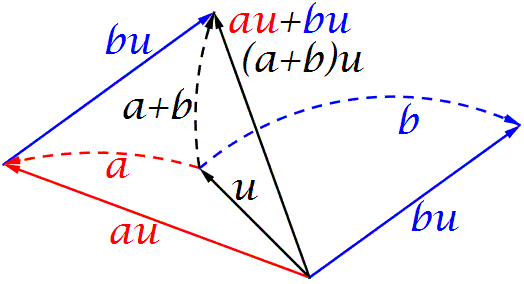
\includegraphics[width=0.5\textwidth]{imagenes/imagenes01/T01IM01.png}
		%\caption{Los dos problemas clásicos del cálculo: trazado de tangentes y áreas bajo curvas.}
	%\end{figure}
		
%varios párrafos encuadrados - explicaciones ad hoc
%\centering{
%\fbox{
%\parbox{0.95\textwidth}{
%varios
%
%$parrafos
%
%dentro
%}
%}
%}
% \justify


%\rotatebox{180}{\leftline{\textcolor{gris}{tararí}}}.

\chapter{Espacios vectoriales $\divideontimes$}	\label{e_vec}

La idea de vector está tomada de la Física, donde sirven para representar magnitudes vectoriales como fuerzas, velocidades o aceleraciones. Para ello se emplean vectores de dos componentes en el plano, de tres componentes en el espacio... 

En Matemáticas, se trata de abstraer las propiedades que caracterizan a los vectores para extenderlas también a otro tipo de objetos diferentes de los vectores de la Física. Esencialmente, el comportamiento que caracteriza a los vectores es el siguiente: 

\hspace{3mm} * Podemos sumar dos vectores y obtenemos otro vector; 

\hspace{3mm} * Podemos multiplicar un vector por un número (escalar) y obtenemos otro vector. 

En álgebra abstracta, un espacio vectorial (o también llamado espacio lineal) es una estructura algebraica creada a partir de un conjunto no vacío, una operación interna (llamada suma, definida para los elementos del conjunto) y una operación externa (llamada producto por un escalar, definida entre dicho conjunto y otro conjunto, con estructura de  cuerpo), con unas propiedades fundamentales.

A los elementos de un espacio vectorial se les llama vectores ($\vec u, \vec v, \vec w, \cdots  $)y a los elementos del cuerpo, escalares ($\alpha, \beta, \gamma, \cdots$).

\section{Espacios vectoriales}

\begin{defi} Se llama `espacio vectorial' $\mathcal V$ sobre un cuerpo $\mathcal K$ a la terna : $\; \; $ \colorbox{LightYellow}{$\displaystyle \left( \; (\mathcal V, \oplus),\; (\mathcal K,+,\cdot),\; \odot \;  \right) $} $\quad$, donde $(\mathcal V, \oplus)$ es un grupo abeliano a cuyos elementos se les llama vectores ($\vec u, \vec v, \vec w, \cdots  $), $(\mathcal K, +, \cdot)$ es un cuerpo conmutativo a cuyos elementos se les llama escalares ($\alpha, \beta, \gamma, \cdots$) y $\odot$ es una ley de composición externa de $\mathcal K$ sobre $\mathcal V$, de modo que $\forall \alpha \in \mathcal K \; \wedge \; \forall \vec u \in \mathcal V \rightsquigarrow \alpha \odot \vec u \in \mathcal V$ , donde se han de cumplir cuatro propiedades:

\begin{enumerate}[EV.1. ]

\item $\lambda \odot (\vec u \oplus \vec v)= (\lambda \odot \vec u) \; \oplus \; (\lambda \odot \vec v)$
\item $(\lambda + \mu)\odot \vec u = (\lambda \odot \vec u) \; \oplus \; (\mu \odot \vec u)$
\item  $(\lambda \cdot \mu)\odot \vec u = \lambda \odot (\mu \odot \vec u)$
\item $1\odot \vec v = \vec v$
$\qquad \qquad \qquad \qquad \forall \lambda, \mu \in \mathcal K; \; \; \forall \vec u, \vec v \in \mathcal V$	
\end{enumerate}
\end{defi}

En adelante usaremos los mismos símbolos para la suma de vectores que de escalares, así como para el producto de escalares y el de un escalar por un vector: $\lambda + \mu; \quad \vec u + \vec v; \quad \lambda \cdot \mu; \quad \lambda \cdot \vec u$ o, simplemente $\lambda \mu; \quad \lambda \cdot \vec u$ o, simplemente $\lambda \vec u$ y también en adelante $\mathcal K \equiv \mathbb R$ y hablaremos de \colorbox{LightYellow}{`espacios vectoriales reales'}, que representaremos más sencillamente por \colorbox{LightYellow}{$(\mathcal V, +, \cdot)$},  donde $+$ es la ley de composición interna en $\mathcal V$, la suma de vectores y $\cdot$  es la ley de composición externa de $\mathbb R$ sobre $\mathcal V$, el producto de un número real (escalar) por un vector.

\begin{ejem}.

\begin{itemize}

\item $\mathbb R; \; \mathbb R^2; \; \mathbb R^3$ y, en general $\mathbb R^n$  son espacios vectoriales reales con las operaciones usuales de ley suma de vectores y producto por un escalar:

$(u_1,u_2,u_3, \cdots, u_n)\; +\; (v_1,v_2,v_3, \cdots v_n)=(u_1+v_1, u_2+v_2, u_3+v_3, \cdots , u_n+v_n)$

 $\alpha \cdot (u_1,u_2,u_3, \cdots, u_n) =(\alpha u_1,\alpha u_2,\alpha u_3, \cdots, \alpha u_n)$

\item $(\mathcal M_{m \times n}(\mathbb R),+,\cdot)$ es el espacio vectorial de las matrices reales de orden $m \times n$ con las operaciones aprendidas en el tema de matrices.

\item $(\mathcal P_n(\mathbb R), +, \cdot)$ es el espacio vectorial de los polinomios de una variable real de grado menor o igual a $n$ con las operaciones habituales de suma de polinomios y producto de un polinomio por un número real.

\item $(\mathcal C_0(\mathbb R), +, \cdot)$ es el espacio vectorial de las funciones reales de variable real `continuas' con las operaciones habituales de suma y producto por un número.
\end{itemize}
\end{ejem}

\begin{prop} Sea $\mathcal V$ un e.v. real, entonces:
\begin{enumerate}[P1. ]
\item $\alpha \; \vec 0=\vec 0,\quad \forall \alpha \in \mathbb R$
\item $0 \; \vec u= \vec 0, \quad \forall \vec u \in \mathcal V$
\item $\alpha \; \vec u = \vec 0 \leftrightarrow \alpha = 0 \; \vee \; \vec u= \vec 0, \quad \forall \alpha \in \mathbb R,\; \forall \vec u \in \mathcal V$
\item $(-\alpha)\; \vec u=-(\alpha \; \vec u)=\alpha\;  (-\vec u),  \quad \forall \alpha \in \mathbb R,\; \forall \vec u \in \mathcal V$
\item $\alpha \; \vec u = \alpha\; \vec v \; \wedge \; \alpha \neq 0 \to \vec u = \vec v, \quad \forall \alpha \in \mathbb R,\; \forall \vec u, \vec v \in \mathcal V$
\item $\alpha \; \vec u = \beta \; \vec u \; \wedge \, \vec u \neq \vec 0 \to \alpha = \beta, \quad \forall \alpha, \beta \in \mathbb R,\; \forall \vec u \in \mathcal V$
\item $(-\alpha)\; (-\vec u)= \alpha \; \vec u , \quad \forall \alpha \in \mathbb R,\; \forall \vec u \in \mathcal V$
	
\end{enumerate}	
\end{prop}


\subsection{Subsespacio vectorial}

\begin{defi}
Sea $\mathcal V$ un espacio vectorial y sea $\mathcal W \subset \mathcal V$ un subconjunto de $\mathcal V$. Decimos que $\mathcal W$ es un `subespacio vectorial de $\mathcal V$' si:

\vspace{2mm}
\centerline{\colorbox{LightYellow}{$\boxed{\; \forall \vec u, \vec v \in \mathcal W \; \wedge \; \forall \lambda, \beta \in \mathbb R \quad \therefore \quad \lambda \vec u + \beta \vec v \in \mathcal W\; }$}}

\end{defi}

\justify

\begin{ejem}
Hay dos subespacios triviales en $\mathcal V$, el mismo 	$\mathcal V$ y $\{\vec 0\}$, se llaman subespacios impropios.

Ejemplos de subespacios vectoriales propios son:

\begin{itemize}
\item $\mathcal V = \mathbb R^2 \to \mathcal W_1= \{\vec 0\} \times \mathbb R; \quad \mathcal W_2= \mathbb R \times \{\vec 0\}$ son subespacios de $\mathbb R^2$

\textcolor{gris}{ \footnotesize{$\alpha (0,x) + \beta (0,y)=(0,\alpha x + \beta y) \in \mathcal W_1 ; \quad 
\alpha (x,0) + \beta (y,0)=(\alpha x + \beta y,0) \in \mathcal W_2 $}}

\item $\mathcal W=\{ (x,0,0) / x \in \mathbb R \} \subset \mathbb R^3$ es s.e.v. de $\mathbb R^3$.
\item $\mathcal W=\{ (x,y,0,t) / x,y,t \in \mathbb R \} \subset \mathbb R^4$ es s.e.v. de $\mathbb R^4$.
\item $\mathcal W=\{ M\in \mathcal M_{n \times n}(\mathbb R) \; / \; A^T=A\}$ es un s.e.v. de $\mathcal M_{n \times n}(\mathbb R)$
\item $\mathcal W=\{ M\in \mathcal M_{2 \times 2}(\mathbb R) \; / \; det(A)=0\}$ NO es un s.e.v. de $\mathcal M_{2 \times 2}(\mathbb R)$

\vspace{2mm} \textcolor{gris}{\small{ya que, p.e., las matrices: 
$A_1=\left( \begin{matrix} 1&0\\0&0 \end{matrix} \right); \quad 
A_2=\left( \begin{matrix} 0&0\\0&1 \end{matrix} \right) \; \in \mathcal W$,}}
 
\textcolor{gris}{ \small{pues $det(A_1)=det(A_2)=0\quad $, pero $A_1+A_2= \left( \begin{matrix} 1&0\\0&1 \end{matrix} \right) \notin \mathcal W$}\normalsize{.}}
	
\end{itemize}
\end{ejem}

\begin{defi}.

Sean $\{ \vec u_1, \vec u_2, \cdots, \vec u_n \} \in \mathcal V$, se llama \colorbox{LightYellow}{`combinación lineal'} de dichos vectores a una expresión de la forma: 
\colorbox{LightYellow}{$\lambda_1 \vec u_1 + \lambda_2 \vec u_2 + \cdots +\lambda_n \vec u_n$},
 donde $\lambda_1, \lambda_2, \cdots, \lambda_n \in \mathbb R$
\end{defi}

\begin{defi}
Dado $\mathcal S \subset \mathcal V$ se define el `subespacio \textbf{generado}' por $\mathcal S$	como el conjunto de todas las combinaciones lineales finitas de elementos de $\mathcal S$, lo representaremos por $\mathcal{L(S)}$:

\vspace{2mm}
\centerline{\noindent \colorbox{LightYellow}{
	$\mathcal {L(S)}= \{\lambda_1 \vec u_1 + \lambda_2 \vec u_2 + \cdots +\lambda_n \vec u_n:\; \lambda_i \in \mathbb R, \; 
	 \vec u_i \in \mathcal V \}$
}\normalsize{.}}

\end{defi}

%\justify

\begin{prop}
Para $	\mathcal S \subset \mathcal V$, el subespacio generado  $\mathcal {L(S)}$ es un subespacio vectorial de $\mathcal V$.
\end{prop}

\begin{proof}.

\noindent \textcolor{gris}{Sean $\alpha, \beta \in \mathbb R$ y $\vec u, \vec v \in \mathcal {L(S)}$, hemos de probar que $\alpha \vec u + \beta \vec v \in \mathcal {L(S)}$.}

\noindent \textcolor{gris}{Por ser $\vec u, \vec v  \in \mathcal {L(S)}$: ,}

\noindent \textcolor{gris}{$\exists a_1, \alpha_2, \cdots, \alpha_n, \beta_1, \cdots , \beta_m \in \mathbb R$ y 
$\exists \vec u_1, \cdots, \vec u_n, \vec v_1, \cdots , \vec v_m \in \mathcal S $, tales que:}

\noindent \textcolor{gris}{$\alpha \vec u + \beta \vec v = \alpha (\alpha_1 \vec u_1 + \cdots + \alpha_n \vec u_n) + \beta (\beta_1 \vec v_1+ \cdots + \beta_m \vec v_m)=$}

\noindent \textcolor{gris}{$= (\alpha \alpha_1) \vec u_1 + \cdots + (\alpha \alpha_n) \vec u_n + (\beta \beta_1) \vec v_1+ \cdots + (\beta \beta_m) \vec v_m $,} 

\noindent \textcolor{gris}{una combinación lineal finita de elementos de $\mathcal S$, luego $\alpha \vec u + \beta \vec v \in \mathcal {L(S)}$}

\end{proof}


\begin{ejem}
Sea $\mathcal S=\{(1,1,1,1),(0,1,1,1)\} \subset \mathbb R^4$. Calculemos $\mathcal {L(S)}.$	

\noindent Un vector $(x,y,z,t) \in \mathcal {L(S)} \leftrightarrow \exists \alpha, \beta \in \mathbb R : \; $

\noindent $(x,y,z,t)= \alpha (1,1,1,1) + \beta (0,1,1,1)= (\alpha, \alpha+\beta, \alpha+\beta, \alpha+\beta) \to $

\noindent SEL: $\begin{cases} x=\alpha \\ y= \alpha+\beta \\ z= \alpha+\beta \\ t= \alpha+\beta \end{cases}\; , \quad $ eliminando parámetros:

\noindent $ A=\left (\begin{matrix} \boxed{1}&\boxed{0}\\\boxed{1}&\boxed{1}\\1&1\\1&1 \end{matrix} \right| 
\left. \begin{matrix} x\\y\\z\\t  \end{matrix} \right) \leftarrow A^*$. Al exigir $rg(A)=2 \to rg(A^*)=2$ (SC),

\noindent se obtiene: $\begin{cases} z-y=0\\t-y=0  \end{cases}, $ es decir:

\noindent $\mathcal {L(S)}= \{ (x,y,z,t)\in \mathbb R^4 \; / \; y=z=t \}$
	

\end{ejem}

\section{Base y dimensión de un e.v.}

\begin{defi}
Dados $\vec u_1, \cdots, \vec u_n \in \mathcal V$, se dice que son \textbf{`linealmente independientes'} (LI)	si dada la combinación lineal:

$\alpha_1 \vec u_1 + \cdots + \alpha_n \vec u_n=\vec 0$, se verifica que $\alpha_1= \cdots =\alpha_n=0$. 

En caso contrario, se dice de los vectores $\vec u_1, \cdots, \vec u_n \in \mathcal V$ son `linealmente dependientes', LD.  
\end{defi}

También se dice que un conjunto de vectores LI es un conjunto de vectores `libres'. Si los vectores sn LD, también se les llama vectores `ligados'.

\begin{ejem}
El vector $\vec 0$ siempre es LD, ya que $\forall \alpha \in \mathbb R:\; \alpha \vec 0 = \vec 0$	
\end{ejem}

\begin{ejem}
$\{(1,0), (1,1)\} \subset \mathbb R^2$ son LI:

\noindent \small{$\alpha (1,0) + \beta (1,1) = (0,0) \to (\alpha+\beta, \beta)=(0,0) \to \begin{cases} \alpha + \beta =0\\ \beta=0 \end{cases} \Rightarrow \alpha=\beta=0$	}\normalsize{.}
\end{ejem}

\begin{ejem}
En $\mathcal P_2(x)$, el e.v. de los polinomios de grado menor o igual a dos de una variable real, el conjunto formado por los `vectores' $\{ 1,x,x^2 \}$ es LI:

Construimos una combinación lineal arbitraria de estos vectores e igualamos a cero (al polinomio-vector cero):	

$\alpha + \beta x + \gamma x^2 =0 \to $ dos polinomios son igules si toman los mismos valores numéricos; para $x=0, x=1, x=-1:$

$\begin{cases} \alpha=0\\ \alpha+\beta+\gamma=0 \\ \alpha+\beta+\gamma=0 \end{cases} \Rightarrow \alpha=\beta=\gamma=0$

\end{ejem}


\begin{prop}
	Si $\vec u_1, \cdots, \vec u_n \in \mathcal V$ son LD, entonces o uno de ellos es $\vec 0$ o es combinación lineal de los restantes.
\end{prop}

\begin{proof}.

\noindent \textcolor{gris}{Si uno de ellos es $\vec 0$, ya hemos acabado. Supongamos, pues, que todos los vectores son no nulos y que en la combinación lineal  $\alpha_1 \vec u_1 + \cdots + \alpha_n \vec u_n=\vec 0$ no todos los escalares son nulos. Supongamos, p.e., que $\alpha_1 \neq 0$:  } 

\noindent \textcolor{gris}{ Despejando: $\vec u_1=-\dfrac{\alpha_2}{\alpha_1}\vec u_2 - \cdots -\dfrac{\alpha_n}{\alpha_1}\vec u_n$, por los que $\vec u_1$ es combinación lineal de los demás.   }
	
\end{proof}

\begin{defi}
Se dice que los vectores $\vec u_1, \cdots, \vec u_n \in \mathcal V$ `generan' $\mathcal V$ si $\mathcal L (\{ \vec u_1, \cdots, \vec u_n \}) = \mathcal V$. En este caso $\mathcal V$ es un espacio vectorial `finito' y  $\{ \vec u_1, \cdots, \vec u_n \}$ es un `sistema generador' de $\mathcal V$.
\end{defi}


\begin{ejem}
El conjunto de vectores 	$\{(1,0), (1,1)\}$ generan el espacio vectorial finito $\mathbb R^2$. Para ello consideremos un vector arbitrario $(x,y) \in \mathbb R^2$ y veamos que existen $\alpha, \beta \in \mathbb R$ tales que $(x,y)=\alpha (1,0)+\beta(1,1)  \longrightarrow \begin{cases} x=\alpha \\ y= \alpha+\beta \end{cases} \Rightarrow \alpha=x \; \wedge \; \beta=y-x$, de modo que 

$(x,y)=x\cdot (1,0)+ (y-x)\cdot (1,1)\; $, y $\; \mathbb R^2 = \mathcal L(\{(1,0), (1,1)\})$
\end{ejem}

\textcolor{gris}{No todos los espacios vectoriales son finitos. Por ejemplo el espacio vectorial de los polinomios de una variable en $\mathbb R$ no es finito; si lo consideramos generado por los vectores $\{1,x,x^2,\cdots ,x^n\}$, el polinomio $x^{n+1}$, p.e., no se puede escribir como combinación lineal de los anteriores.}

\begin{prop}
Sea $\mathcal S=\{\vec u_1, \cdots, \vec u_n \}$ un sistema generador de $\mathcal V$. Entoces existe $\mathcal B \subset \mathcal S$	 que también genera $\mathcal V$ y cuyos vectores son LI.
\end{prop}

\begin{prop}
Supongamos que $\mathcal V$ está generado por $n$ vectores. Entonces, ningún conjunto LI de vectores de $\mathcal V$ tiene más de $n$ elementos.	
\end{prop}

\begin{defi} \colorbox{LightYellow}{ Una \textbf{`base'} de $\mathcal V$ es un sistema de generadores de $\mathcal V$}

\noindent \colorbox{LightYellow}{cuyos vectores son LI   }	
\end{defi}
 
\begin{ejem}.

--- $B=\{1,x,x^2\}$ es una base de $\mathcal P_2(x)$, espacio vectorial de los polinomios reales de una variable de grado menor o igual a dos.	

--- $B= \left\{\; 
\left(\begin{matrix} 1&0\\0&0\end{matrix} \right);\;
\left(\begin{matrix} 0&1\\0&0 \end{matrix} \right);\;
\left(\begin{matrix} 0&0\\1&0\end{matrix} \right); \; 
\left(\begin{matrix} 0&0\\0&1 \end{matrix} \right) \;\right\}$ es una base de $\mathcal M_{2 \times 2}(\mathbb R)$, espacio vectorial de las matrices reales cuadradas de orden dos.

--- $B=\{(1,0), (1,1)\}$ es una base de $\mathbb R^2$.
\end{ejem}

\begin{teor} En un espacio vectorial finito $\mathcal V$, todas las bases tienen el mismo número de vectores.	
\end{teor}

\begin{proof}.

\noindent \textcolor{gris}{ Sean $B_1=\{ \vec u_1, \cdots , \vec u_n\}$ y  $B_2=\{ \vec v_1, \cdots , \vec v_n\}$   dos bases de $\mathcal V$. Como una base es un sistema generador libre (LI), tanto $B_1$ como $B_2$ son sistemas de generadores. Si consideramos $B_1$ como sistema de generadores y $B_2$ como base, por la proposición anterior se tendría que $n\ge m$. Si consideramos $B_2$ sistema generador y $B_1$ base, entonces $m\ge n$, por lo que $m=n$. }
	
\end{proof}

\begin{defi}
Dado $\mathcal V$ un espacio vectorial finito, se	llama \textbf{`dimensión'} de  $\mathcal V$,  $dim(\mathcal V)$, al número de vectores de una cualquiera de sus bases.
\end{defi}


\begin{prop}
Sea $B=\{\vec u_1, \cdots, \vec u_n \}$ una base de $\mathcal V$. Entonces, todo vector $\vec u \in \mathcal V$ se escribe de `forma única'	como combinación lineal de los vectores de esa base $B$
\end{prop}

\begin{proof}

\noindent \textcolor{gris}{Supongamos que $\vec u$ admite dos formas distintas de expresarse como combinación lineal de vectores de $B$:  }	

\noindent \textcolor{gris}{$\vec u=\alpha_1 \vec u_1+ \cdots + \alpha_n \vec u_n=\beta_1 \vec u_1+ \cdots + \beta_n \vec u_n $, entonces   }	

\noindent \textcolor{gris}{$(\alpha_1-\beta_1) \vec u_1+\cdots + (\alpha_n-\beta_n) \vec u_n= \vec 0$, como los vectores de $B$ son LI:   }	

\noindent \textcolor{gris}{$\alpha_i - \beta_i=0,\; \forall i\in \{1, \cdots, n\}$, es decir, $\alpha_i=\beta_i, \; \forall i$, por lo que ambas formas son la misma y $\vec u$ solo se puede escribir de una forma única en la base $B$.   }	

\end{proof}

Esta es una de las ventajas de la estructura de espacio vectorial, que todo vector del espacio, fijada una base, se puede escribir en ella de forma única.

Dada una base $B=\{\vec u_1, \cdots, \vec u_n \}$ de un e.v. real $\mathcal V$, $\forall \vec u \in \mathcal V, \; \exists !\; (\alpha_1, \cdots , \alpha_n )$

\vspace{-2mm} \noindent $\in \mathbb R$ de modo que $\vec u$ se escribe en $B$ de forma única:
$\vec u=\alpha_1 \vec u_1+ \cdots + \alpha_n \vec u_n$, decimos que $(\alpha_1, \cdots, \alpha_n)$ son las \textbf{`componentes'} de $\vec u$ en la base $B$.

Hay que notar que si en $\mathcal V$ cambiamos de base, cambian las componentes de cualquier vector $\vec u$. Veamos un ejemplo:

$B=\{ \vec e_1=(1,0),\; \vec e_2=(0,1)\}$ base de $\mathbb R^2$. Consideremos el vector $\vec u=1\cdot \vec e_1+ 1 \cdot \vec e_2=(1,0)+(0,1)=(1,1)$. Decimos que $\vec u$, expresado en $B$ tiene por componentes $(1,1)$, que denotaremos así: $\vec u=(1,1)_B$

Veamos como escribir este mismo vector $\vec u \in \mathbb R^2$ en una nueva base $B'=\{ \vec u_1=(1,1),\; \vec u_2=(1,-1)\}$: 

\noindent $\vec u=(1,1)=\alpha u_1+\beta \vec u_2=\alpha (1,1)+\beta (1,-1)=(\alpha+\beta, \alpha-\beta)\to $

\noindent $\to \begin{cases} \alpha+\beta=1 \\ \alpha-\beta=1 \end{cases} \to \alpha=1\; \wedge \; \beta =0 \Rightarrow \vec u=(1,0)_{B'} $

En una tercera base $B''=\{(1,0),(1,-1)\} \to $

\noindent $(1,1) =  \lambda_1 (1,0) + \lambda_2 (1,-1) \to \begin{cases} \lambda_1 +\lambda_2=1 \\ -\lambda_2=1 \end{cases} \lambda_1=2\;\wedge \; \lambda_2=-1  $

\noindent y entonces: $\vec u=(2,1)_{B''}$

La base $B$ la llamaremos `base canónica' pues las coordenadas de un vector son las \emph{naturales} en $\mathbb R^2$. Así, todo vector de $\mathbb R^n:\; \vec u= (x_1, \cdots, x_n)$ tiene por coordenadas $(x_1, \cdots, x_n)_C$ respecto de la base canónica $C=\{(1,0,\cdots ,0),(0,1,\cdots, 0) \cdots , (0,0,\cdots ,1)\}$. En el e.v. $\mathcal P_n(x)$, la base canónica es: $C=\{ 1,x,x^2, \cdots, x^n\}$, así, cualquier polinomio $p(x)=a_0+a_1x+a_2x^2+ \cdots + a_nx^n$ tiene por componentes $(a_0,a_1,a_2, \cdots , a_n)_C$.

\begin{teor}
Sea $\mathcal V$ un espacio vectorial real de dimensión finta (e.v. finito) de dimensión $n$. Entonces:

\vspace{-4mm}
\begin{enumerate}[a) ]	
\item Todas las bases de $\mathcal V$ tienen $n$ elementos.
\item Todo conjunto LI de $n$ elementos es una base en $\mathcal V$.
\item Todo sistema generador de $\mathcal V$ de $n$ elementos es una base.	
\end{enumerate}

\end{teor}



\subsection{Rango de un conjunto de vectores}

\begin{defi}
Sea $S=\{ \vec u_1, \cdots , \vec u_n \}$ un conjunto de vectores de un e.v. $\mathcal V$ y sea $W=\mathcal L(\{ \vec u_1, \cdots , \vec u_n \})$ un subespacio vectorial generado por $S$.

Se llama \textbf{`rango'} del conjunto de vectores $S$, $rg(S)$ a la dimensión del subespacio $W$ generado por $S$: $rg(S)=dim(W)=dim(\mathcal L(S))$
\end{defi}

Según lo visto hasta ahora, $rg(S)=$ máximo número de vectores LI de S.

\begin{teor}

Sea  $S=\{ \vec u_1, \cdots , \vec u_n \}$ un conjunto de vectores y $W=\mathcal L(S)$ el subespacio vectorial engendrado por estos.

Sea $S'$ el conjunto de vectores obtenido al aplicar a $S$ las transformaciones de Gauss necesarias para transformar a $S$ en un sistema escalonado (ver \ref{escalonado} en tema de  5 del teorema de Rouché).

Entonces:


$a)\; S'$ engendra el mismo subespacio $W$ que $S$.
$\quad b)\; rg(S')=rg(S)$	


\end{teor}

Veamos un ejemplo:

\noindent \small{$S=\{\vec u_1=(1,1,2,0); \; \vec u_2=(2,-1,0,1); \; \vec u_3=(5,-1,2,2); \; \vec u_4=(3,0,2,1) \}$} \normalsize{ y} sea $W=\mathcal L(S)$ el subespacio vectorial generado por $S$.

\noindent Escribamos las coordenadas de los vectores de $S$ como filas de una matriz y escalonémosla:

\noindent $\left (\begin{matrix}  \vec u_1=(1,1,2,0) \\ \vec u_2=(2,-1,0,1) \\ \vec u_3=(5,-1,2,2) \\ \vec u_4=(3,0,2,1) \end{matrix} \right) \to \left (\begin{matrix} \vec v_1= \vec v1 &= (1,1,2,0) \\ \vec v_2=\vec u_2-2\vec u_1 &=(0,-3,-4,1) \\ \vec v_3=\vec u_3-5\vec u_1 &=(0,-6,-8,2) \\ \vec v_4=\vec u_4-3\vec u_1 &=(0,-3,-4,1)    \end{matrix} \right) \to $

\noindent $\to \left (\begin{matrix} \vec w_1=\vec v1 &=(1,1,2,0) \\ \vec w_2=\vec v_2 &=(0,-3-4,1) \\ \vec w_3=\vec v_3-2\vec v_2 &=(0,0,0,0) \\ \vec w_4=\vec u_4-\vec u_2 &=(0,0,0,0) \end{matrix} \right)$ Los vectores $\vec w_1, \vec w_2$ son LI, por lo que $rg(S)=2$.

\noindent Además, como generan el mismo $W$, $B_W=\{(1,1,2,0), (0,-3-4,1) \}$

\noindent Si $\vec x=(x_1,x_2,x_3,x_4) \in W \to \vec x=\alpha \vec w_1 + \beta \vec w_2 = $

\noindent $=\alpha (1,1,2,0) + \beta (0,-3-4,1)=(\alpha , \alpha-3\beta, 2\alpha-4\beta, \beta) \to $

\noindent \small{$\to (*)\; \begin{cases} x_1=\alpha \\ x_2= \alpha-3\beta \\ x_3= 2\alpha-4\beta \\ x_4= \beta  \end{cases}$} \normalsize{se} llaman \textbf{ecuaciones paramétricas de W}, 
al tomar $\alpha$ y $\beta$ todos los valore posibles se obtienen todos los vectores de $W$.

\noindent Por ejemplo, tomando $\alpha=2$ y $\beta=-3$ se obtiene el vector $\vec y=(2,11,16,3) \in W$ que lo  podemos escribir como $\vec y=(2,-3)_{B_W}$

\noindent Al eliminar en $(*)$ los parámetros: $A=\left( \begin{matrix} \boxed{1}&\boxed{0}\\1&-3\\2&-4\\\boxed{0}&\boxed{1} \end{matrix} \right| \left. \begin{matrix} x_1\\x_2\\x_3\\x_4 \end{matrix} \right) \leftarrow A^*$, exigiendo que $rg(A)=2=rg(A^*)$, obtenemos: $\begin{cases} x_2=x_1-3x_4\\x_3=2x_1-4x_4 \end{cases}$ que son las \textbf{ecuaciones implícitas} de $W$, las condiciones (restricciones) que tienen que cumplir los vectores $(x_1,x_2,x_3,x_4) \in \mathbb R^4$ para ser vectores de $W$.



\noindent Se cumple que:

--- \emph{dim. subespacio = dim. espacio - núm. restricciones} \tiny{(2=4-2)}\normalsize{.}

--- El rango de un conjunto de vectores de $\mathbb R^n$ es siempre menor o igual a $n$.

--- Si el rango de un conjunto de vectores $S$ de $\mathbb R^n$ es $n$, esos vectores LI de $S$ son una base de $\mathbb R^n$.

\subsection{Cambio de base}
\label{matriz-cambio-base}

\begin{teor}{Cambio de base en $\mathbb R^n$}.

Si $B$ es una base de $\mathbb R^n$, y $\vec x$ un vector cuyas componentes en $B$ son $(x'_1,\cdots ,x'_n)_B$, escribiremos el vector  $\vec x$  como vector fila:

 $\vec x =\left( x'_1, x'_2, \cdots x'_n \right)_B $ 
 
 Este mismo vector, en la base canónica $C=\{\; \vec e_1=(1,0,\cdots ,0),\vec e_2=(0,1,\cdots, 0) \cdots , \vec e_n=(0,0,\cdots ,1)\; \}$ de $\mathbb R^n$ lo escribiremos  por sus componentes naturales $(x_1,\cdots ,x_n)$ como vector fila:
 
  $\vec x =\left( x_1, x_2, \cdots , x_n \right)_C $.
  
  Si $B=\{\vec u_1, \cdots , \vec u_n\}$, cuyos vectores escritos en $C$ tienen por componentes $\vec u_i=\alpha_{1i} (1,0,\cdots ,0) + \alpha_{2i}(0,1,\cdots, 0)+ \cdots + \alpha_{1n}(0,0,\cdots ,0)$, entonces, se puede demostrar \textcolor{gris}{(es sencillo)} que:
  
 \noindent  \small{$\boldsymbol{\vec {x_C}} = (x_1, x_2, \cdots, x_n) = (x'_1, x'_2, \cdots , x'_n) \cdot\left( \begin{matrix} 
  \alpha_{11} & \alpha_{12}&\cdots & \alpha_{1n} \\
  \alpha_{21} & \alpha_{22}& \cdots & \alpha_{2n} \\
  \vdots & \cdots &\ddots & \vdots \\
  \alpha_{n1} & \alpha_{n2}& \cdots & \alpha_{nn}
  \end{matrix} \right) =\boldsymbol{ \vec {x_B} \cdot A }$} 

\normalsize{Donde} $A$ es la matriz de cambio de la base $B$ a la base $C$. Para pasar de $C$ a $B$ usaríamos la matriz inversa $A^{-1}: \quad \boldsymbol{\vec{x_B}=\vec {x_C}\cdot A^{-1} }$ (Es costumbre escribir los vectores como matrices columna en vez de matriz fila, entonces la matriz de cambio de base es $A^T$).
  
\end{teor}

\begin{ejem}
Sea $B=\{(1,1,1),(1,2,0),(0,0,1)\}$ una base de 	$\mathbb R^3$, entonces, el vector $\vec x)=(1,1,1)_B=1\cdot (1,1,1)+1\cdot (1,2,0)+ 1 \cdots(0,0,1)=(2,3,2)_C$, se puede obtener, matricialmente como:

$(2,3,2)_C= (1,1,1)_B \cdot \left( \begin{matrix} 1&1&1\\1&2&0\\0&0&1 \end{matrix} \right)$, siendo \scriptsize{$\left( \begin{matrix} 1&1&1\\1&2&0\\0&0&1 \end{matrix} \right)$} \normalsize{la} matriz de cambio de base.

\textcolor{gris}{$\left( \begin{matrix} 2\\3\\2 \end{matrix} \right)_C = 
\left( \begin{matrix} 1&1&0\\1&2&0\\1&0&1 \end{matrix} \right) \cdot 
\left( \begin{matrix} 1\\1\\1 \end{matrix} \right)_B$, escrito como vectores columna.}
\end{ejem}

\begin{teor}
Si $A_{BC}$ es la matriz de cambio de base de $B$ a $C$ y $B'$ es otra base, entonces:

\vspace{-4mm}
\begin{enumerate}[a) ]	
\item $\exists {(A_{BC})}^{-1}=A_{CB}$
\item $A_{B'B}=A_{CB}A_{B´C}=A^{-1}_{BC}A_{B'C}$	
\end{enumerate}

\end{teor}


\section{Ejercicios resueltos}

\begin{ejre}
Comprueba que $(2,1,-3)$ es combinación lineal de los vectores $	(1,-1,1),\; (1,0,0),\; (1,1,0)$
\end{ejre}
\begin{proofw}\renewcommand{\qedsymbol}{$\diamond$}

Si lo dicho en el enunciado es cierto, deben existir $\alpha, \; \beta, \; \gamma \; \in \mathbb R$, tales que:

\noindent $(2,1,-3)=\alpha (1,-1,1)+  \beta (1,0,0)+ \gamma (1,1,0)=(\alpha+\beta+\gamma, \; -\alpha+\gamma,\; \alpha) \to$

\noindent $\alpha=-3; \; \gamma=-2; \; \beta=7 \Rightarrow $


\noindent Efectivamente, el vector $(2,1,-3)$ es combinación lineal de los otros tres pues lo hemos podido escribir como:

\noindent $ \Rightarrow (2,1,-3)=\boxed{-3}\;  (1,-1,1)+  \boxed{7}\;  (1,0,0)+ \boxed{-2}\;  (1,1,0)$
\end{proofw}


\begin{ejre}
Comprueba que $S=\{ (1,-1,1),\; (1,0,0),\; (1,1,0) \}$ es un sistema libre, LI (linealmente independiente) de vectores de $\mathbb R^3$	.
\end{ejre}
\begin{proofw}\renewcommand{\qedsymbol}{$\diamond$}
	Si ello es cierto, cualquier combinación lineal de los tres vectores igualada a $\vec 0$ debe implicar que todos los escalares de la combinación sean nulos:

\noindent $\alpha (1,-1,0)+\beta (1,0,0) +\gamma (1,1,0)=(0,0,0) \; \to \; \begin{cases}  \; \alpha+\beta+\gamma=0\\ -\alpha+\gamma=0\\ \; \alpha=0 \end{cases} \rightarrow \cdots \to \alpha=\beta=\gamma=0$, efectivamente los tres vectores de $S$ son LI.
	
\end{proofw}


\begin{ejre}
	Demostar que $S=\{ (1,-1,1),\; (1,0,0),\; (1,1,0) \}$ forma una base de $\mathbb R^3$ y encontrar las componentes del vector $\vec v=(2,-1,3)$ en la base $S$.
\end{ejre}
\begin{proofw}\renewcommand{\qedsymbol}{$\diamond$}
	Una base es un SG (sistema de generadores) que sea LI (linealmente independiente). Esto último lo acabamos de demostrar en el problema anterior(*). Veamos ahora que $S$ es un SG de $\mathbb R^3$: debe ocurrir que cualquier vector $(a, \; b, \; c)$ de $\mathbb R^3$ se pueda escribir de `manera única' como combinación lineal de los vectores de $S$, entonces,

\noindent $(a, \; b, \; c)=\alpha (1,-1,1)+  \beta (1,0,0)+ \gamma (1,1,0)=(\alpha+\beta+\gamma, \; -\alpha+\gamma,\; \alpha) \to$

\noindent $\begin{cases} \; \alpha+\beta+\gamma&=a\\ -\alpha+\gamma&=b\\ \; \alpha&=c \end{cases} \to \left( \begin{matrix} 1&1&1\\-1&0&1\\1&0&0 \end{matrix} \right)\cdot \left( \begin{matrix} \alpha \\ \beta \\ \gamma \end{matrix} \right)=\left( \begin{matrix} a \\ b \\c \end{matrix} \right) \leftrightarrow AX=B$

\noindent Como $|A|\neq 0 \to rg(A)=3=rg(A^*)=$ núm. incóg $\to$ SCD (sistema compatible determinado), es decir, existe una solución única, una solo forma de escribir $(a,b,c)_C=(\alpha,\beta,\gamma)_S$, donde $C$ es la base canónica de $\mathbb R^3$. Luego $S$ es un SG de  $\mathbb R^3$. $\qquad \Box$

\noindent En el caso de $\vec v=(2,-1,3)=(2,-1,3)_C$, reemplazando $a=2, \; b=-1, \; c=3$ en el SEL (sistema de ecuaciones lineales) anterior, obtenemos (como ya lo hacíamos en el ejercicio 1):  $\quad \alpha=-3; \; \gamma=-2; \; \beta=7 \; \Rightarrow  \; \vec v=(2,-1,3)_C=(-3,7,-2)_S$
	
	
\noindent \textcolor{gris}{(*) Otra forma de comprobar que $S$ es un sistema LI es estudiando el rango de la matriz formada por los tres vectores de $S$ escritos como filas.}

\noindent \textcolor{gris}{Efectivamente: $\left| \begin{matrix} 1&-1&1 \\ 1&0&0 \\ 1&1&0 \end{matrix} \right| =1 \neq 0 \to rg(S)=3$ y los tres vectores de $S$ son LI}


\end{proofw}


\begin{ejre}
	Comprobar si los siguientes conjuntos tienen estructura de subespacio vectorial:
	
	$A=\{\; (x,y)\in \mathbb R^2 \; :\quad x+y=1\;\} $
	
	$B=\{\; (x,y,z)\in \mathbb R^3 \; : \quad x+y+z=0\;\} $
	
	$C=\{\;(x,y,z)\in \mathbb R^3 \; : \quad x\cdot y=0 \;\} $
	
\end{ejre}
\begin{proofw}\renewcommand{\qedsymbol}{$\diamond$}.

--- $A=\{\; (x,y)\in \mathbb R^2 \; :\quad x+y=1\;\} $

\noindent Veamos un contraejemplo \textcolor{gris}{(ejemplo que demuestra la falsedad de lo que se pretende demostrar)}: $(1,0), (2,-1) \in A \to$ (la suma de sus componentes da uno) la combinación lineal $(1,0) +( 2,-1)=(3,-1) \notin A$, ya que $3+(-1)=2\neq 1$. Luego $A$ no es suebespacio vectorial de $\mathbb R^2$
	
--- $B=\{\; (x,y,z)\in \mathbb R^3 \; : \quad x+y+z=0\;\} $

\noindent Sean $\alpha, \beta \in \mathbb R$ y $(x_i,y_i,z_i) \in B:\; x_i+y_i+z_i=0,\; i=1,2$, entonces la combinación lineal general: 

\noindent $\alpha (x_1,y_1,z_1)+\beta (x_2,y_2,z_2)=\left(\;  (\alpha x_1+\beta x_2, \alpha y_1+\beta y_2, \alpha z_1+\beta z_2)\; \right)$ pertenecerá a $B$ sí la suma de sus componentes es nula:

\noindent $\alpha x_1+\beta x_2\; +\; \alpha y_1+\beta y_2 \; +\; \alpha z_1+\beta z_2 = \alpha(x_1+y_1+z_1)+\beta (x_2+y_2+z_2)=\alpha \cdot 0 + \beta \cdot 0=0$. Luego $B$ sí es un subespacio vectorial de $\mathbb R^3$
	
--- $C=\{\;(x,y,z)\in \mathbb R^3 \; : \quad x\cdot y=0 \;\} $

\noindent Veamos un contraejemplo: Sean $\vec u=(1,0,1)$ y $\vec v=(0,1,0)$. $\vec u, \vec v \in C$, ya que el producto de primera por segunda componentes son nulas, pero $\vec w=\vec u + \vec v =(1,1,1)\notin C$, ya que $w_x\cdot w_y=1\cdot 1 = 1 \neq 0$, por lo que $C$ no es subespacio vectorial de $\mathbb R^3$.
	
\end{proofw}


\begin{ejre}
	Sea $W$ el subespacio vectorial de $\mathbb R^3$ generado por los vectores $\vec u=(1,0,1) \text{ y } \vec v=(1,1,1)$. Determínese una base de $W$, así como las ecuaciones paramétricas e implícitas de $W$.
\end{ejre}
\begin{proofw}\renewcommand{\qedsymbol}{$\diamond$}
	$W=\mathcal L \left( \{\; \vec u=(1,0,1); \; \vec v=(1,1,1) \; \} \right)$
	
\noindent $rg \left( \begin{matrix} 1&1\\0&1\\1&1 \end{matrix} \right)=2 \to $ forman una base $B_W=\{\vec u, \vec v\}$ y  $dim W=2$

\noindent $(x,y,z)\in W \to (x,y,z)=\lambda (1,0,1)+\mu (1,1,1)=(\lambda+\mu, \mu, \lambda+\mu) \to \begin{cases} x&=\lambda+\mu \\y&=\mu\\ z&= \lambda+\mu \end{cases}$ Ecuaciones paramétricas de $W$.

\noindent Eliminando parámetros, $rg \left( \begin{matrix} 1&1&x\\0&1&y\\1&1&z \end{matrix} \right)=2 \to z-x=0$ Ecuación implícita de $W$, es decir, $W=\{\; (x,y,z)\in \mathbb R^3\; : \quad z-x=0 \; \}$

\end{proofw}


\begin{ejre}
	Encuentra el rango de la matriz \footnotesize{$A=\left( \begin{matrix} 1&2&-4&3\\2&5&-3&4\\6&17&-7&10\\1&3&-3&2 \end{matrix} \right)$}\normalsize{.} Encuentra una base del subespacio generado por los vectores fila de la matriz A, así como las ecuaciones paramétricas e implícitas de dicho subespacio.
\end{ejre}
\begin{proofw}\renewcommand{\qedsymbol}{$\diamond$}
	Escalonando por Gauss: $\left( \begin{matrix} 1&2&-4&3\\2&5&-3&4\\6&17&-7&10\\1&3&-3&2 \end{matrix} \right) \to \cdots \to -2\beta+2\gamma\left( \begin{matrix} 1&2&-4&3\\0&1&5&-2\\0&0&8&2\\0&0&0&0\end{matrix} \right)$, por lo que, como $rg(A)=3 \to  dim\; \mathcal L(A)=3$ y los tres primeros vectores fila de $A$, o mejor aún, de $A_e$ (forma escalonada de $A$) forman una base: $B_A=\{ (1,2,-4,3),(0,1,5,-2),(0,0,8,2) \}$

\noindent Cualquier vector de $A.\; (x,y,z,t) $ se podrá escribir en función de los vectores de $B_A$ de forma única:

\noindent $ (x,y,z,t)=\alpha (1,2,-4,3) + \beta (0,1,5,-2) +\gamma (0,0,8,2) \to$

\noindent $ \begin{cases}x=\alpha \\ y=2\alpha+\beta \\z=-4\alpha+5\beta+8\gamma \\ t=3\alpha-2\beta +2\gamma \end{cases} $, que son las ec. paramétricas de $A$

\noindent Al eliminar ls parámetros: $\left( \begin{matrix} 1&0&0 \\ 2&1&0 \\ -4&5&8 \\ 3&-2&2 \end{matrix} \right| \left. \begin{matrix} x\\y\\z\\t \end{matrix} \right) \to \left| \begin{matrix} 1&0&0&x \\ 2&1&0&y \\ -4&5&8&z \\ 3&-2&2&t \end{matrix} \right|=0 \Rightarrow 14x-3y-z-4t=0   $, que es la ecuación implícita de $A$.
\end{proofw}



\begin{ejre}
	Dadas las bases de $\mathbb \; R^3\; : $ 

\noindent $B=\{ \vec u_1=\textcolor{red}{(2,1,0)}, \vec u_2=\textcolor{blue}{(-1,0,1)}, \vec u_3=\textcolor{ForestGreen}{(0,1,-2)} \} \text{\;  y } $

\noindent $B'=\{ \vec v_1=(0,1,1), \vec v_2=(1,0,0), \vec v_3=(2,0,1) \}$, encontrar la matriz que permite cambiar de la base $B$ a la $B'$. Si $\vec w=(1,1,1)$ en la base $B$, ¿cómo se escribe en la base $B'$?
\end{ejre}

\begin{proofw}\renewcommand{\qedsymbol}{$\diamond$}
	Trabajaremos con vectores fila.
	
\noindent $\vec w_B=(1,1,1)_B=1\cdot \vec u_1 +1\cdot \vec u_2 +1\cdot \vec u_3 =(2,10)+(-1,0,1)+(0,1,-2)=(1,2,-1)_C$, siendo $C$ la base canónica de $\mathbb R^3$ \textcolor{gris}{  $\; (\;C=\{ \vec e_1=(1,0,0), \vec e_2=(0,1,0), \vec e_3=(0,0,1) \}\;) $   }

\noindent Si escribimos los vectores de la base $B$ (expresados en la base canónica $C$) como vectores fila, obtenemos la matriz $A_{BC}$ de cambio de base de vectores en $B$ a vectores expresados en $C$:

\noindent $ A_{BC}=\left( \begin{matrix} \textcolor{red}{2}&\textcolor{red}{1}&\textcolor{red}{0}\\ \textcolor{blue}{-1}&\textcolor{blue}{0}&\textcolor{blue}{1}\\ \textcolor{ForestGreen}{0}&\textcolor{ForestGreen}{1}&\textcolor{ForestGreen}{-2} \end{matrix} \right) $ , matriz de cambio de base de $B$ a $C$, dado un vector en B, $\vec w_B$, para escribirlo en $C$, $\vec w_C$, bastará con aplicar la ecuación matricial: $\;\boldsymbol{ \vec w_C=\vec w_B \cdot A_{BC} } \; $ (1*).

\noindent \small{Comprobémoslo: $\vec w_C=\vec w_B \cdot A_{BC}=(1,1,1)_{\cancel{B}}\cdot \left( \begin{matrix} 2&1&0\\-1&0&1\\0&1&-2\end{matrix} \right)_{\cancel{B}C}=(1,2,-1)_C$}\normalsize{.}

\noindent Analogamente tenemos $\left( \begin{matrix} 0&1&1\\1&0&0\\2&0&1 \end{matrix} \right)=A_{B'C} $, es la matriz de cambio de la base $B'$ a la base $C$, así: $\boldsymbol{  \vec w_c=\vec w_{B'}\cdot A_{B'C} }\; $ (2*)

\noindent Las expresiones (1*) y (2*) y el hecho de saber que las matrices de cambio de base (rango 3, en este caso, luego determinante distinto de cero) son invertibles nos permetirán encontrar la ecuación de cambio de base de B a B':

\noindent $\vec w_c=\vec w_{B'}\cdot A_{B'C} \to  \vec w_c \cdot (A_{B'C})^{-1}=\vec w_{B'}\cdot A_{B'C} \cdot (A_{B'C})^{-1} \vec w_{B'} \cdot I=   \vec w_{B'} $

\noindent Es decir, $\vec w_{B'} = \vec w_c \cdot (A_{B'C})^{-1}$

\noindent Como $\vec w_C=\vec w_B \cdot A_{BC} \to \vec w_{B'}=(\vec w_B \cdot A_{BC} )\cdot {(A_{B'C})}^{-1}= \vec w_{B}\cdot A_{BC}\cdot A^{-1}_{B'C}=\vec w_B \cdot A_{BB'}\;$, con $\;A_{BB'}= A_{BC}\cdot A^{-1}_{B'C}\;$, la matriz de cambio de base de vectores expresados en $B$ a vectores expresados en $B'$

\noindent Por adjuntos, podemos calcular $A^{-1}_{B'C}={(A_{B'C})}^{-1}= \left( \begin{matrix} 0&1&0\\1&2&-1\\0&-2&1 \end{matrix} \right)$

\noindent La matriz de cambio de base de $B$ a $B'$, $A_{BB'}$, será:

\noindent $A_{BB'}= A_{BC}\cdot A^{-1}_{B'C}=\left( \begin{matrix} 2&1&0\\-1&0&1\\0&1&-2\end{matrix} \right) \cdot \left( \begin{matrix} 0&1&0\\1&2&-1\\0&-2&1 \end{matrix} \right) = \left( \begin{matrix} 1&4&-1\\0&3&1\\1&6&-3 \end{matrix} \right)$

\noindent Con esto, la expresión de $\vec w$ que en $B$ es $(1,1,1)$, en $B'$ tendrá por componentes:

\noindent $\vec w_{B'}=\vec w_{B} \cdots A_{BB'}= (1\; 1\; 1) \cdot \left( \begin{matrix} 1&4&-1\\0&3&1\\1&6&-3 \end{matrix} \right) = (2,7,-3)$

\noindent Finalmente: $\vec w= (1,1,1)_B=(1,2,-1)_C=(2,7,-3)_{B'}$

\noindent \textcolor{gris}{Comprobación: $(1,1,1)_B=(1,2,-1)_C=(\alpha, \beta, \gamma)_{B'}=\alpha \vec v_1 + \beta \vec v_2 + \gamma \vec v_3 = \alpha (0,1,1)+\beta(1,0,0)+\gamma (2,0,1)=(\beta+2\gamma, \alpha, \alpha+\gamma)_C \to $}

\noindent \textcolor{gris}{$\begin{cases} \beta+2\gamma =1 & \to \quad \to \beta =7\\
 \alpha = 2\\
 \alpha + \gamma =-1 & \to \gamma =-3 \end{cases}  \to \vec w_{B'}=(2,7,-3)_{B'}\qquad \qquad  \Box$}	
 
 Si admitimos la notación $A^{-1}_{B'C}=A_{CB'}$, y siendo $A_{BC} y A_{B'C}$ las matrices de cambio de base de $B$ y $B'$ a la base canónica $C$, respectivamente, podemos escribir:
 $\qquad A_{BB'}=A_{B\cancel{C}}\cdot A_{\cancel{C}B'} \textcolor{gris}{= A_{BC}\cdot A^{-1}_{B'C}}$

\end{proofw}

\begin{figure}[H]
	\centering
	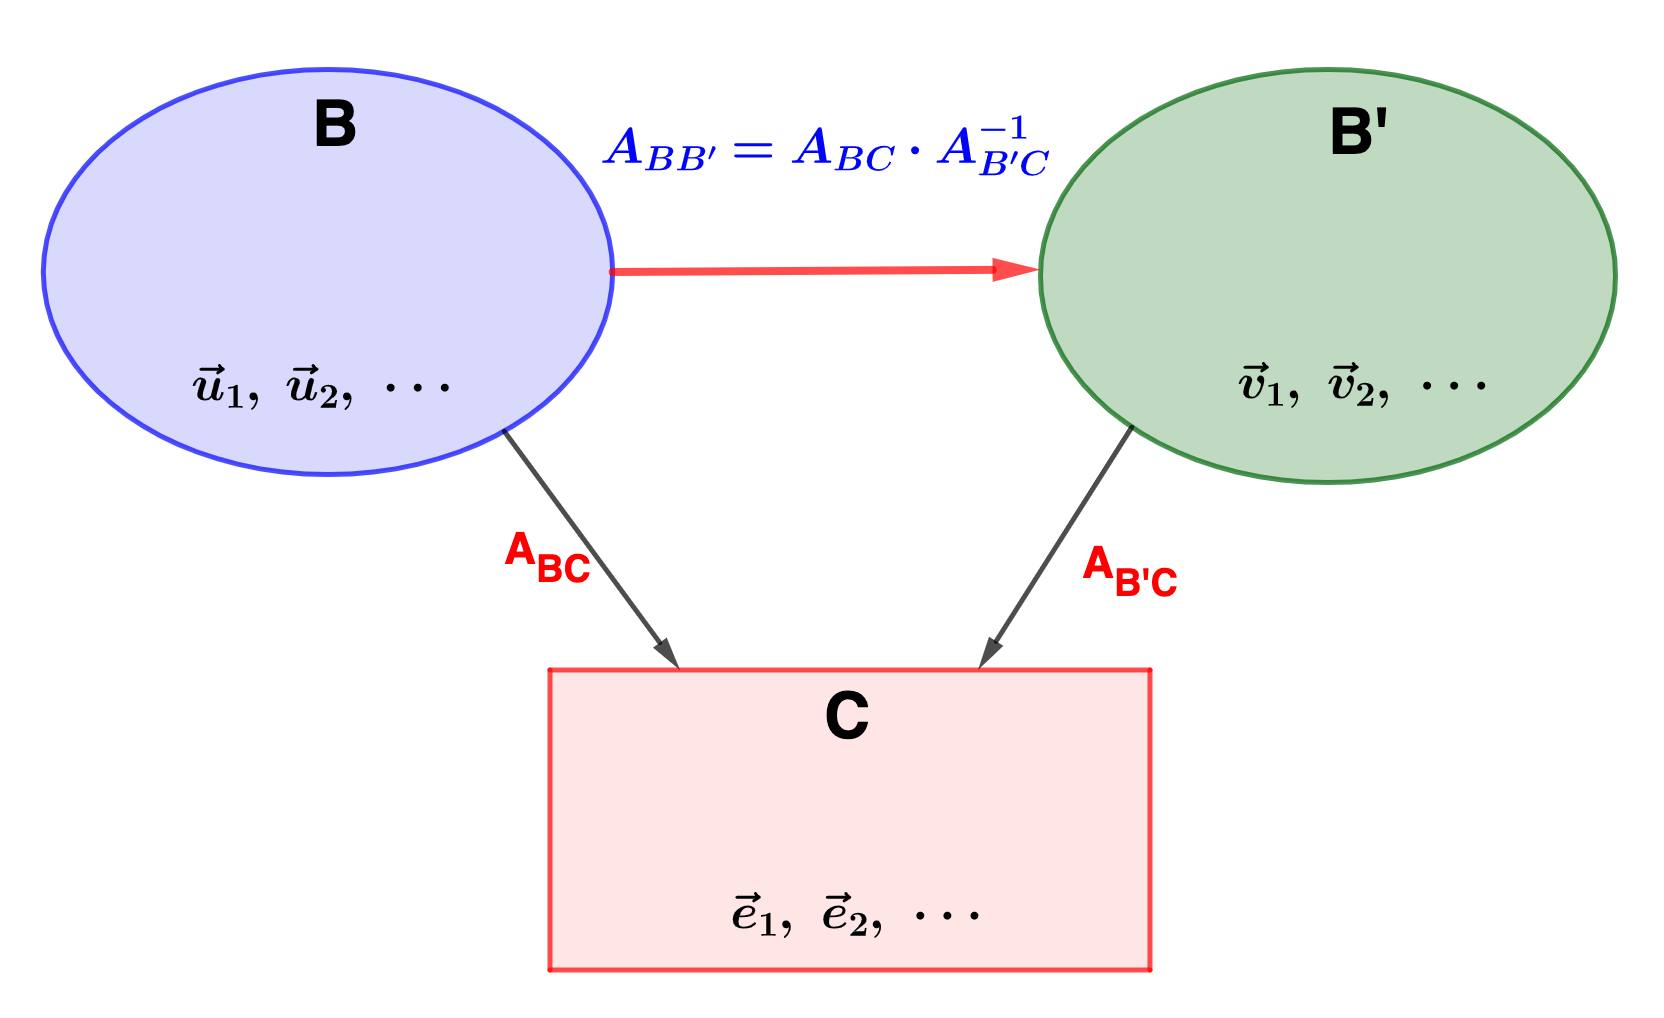
\includegraphics[width=0.7\textwidth]{imagenes/imagenes06/T06IM01.png}
		\caption*{Matriz de cambio de base.}
\end{figure}


\begin{myexampleblock}{Historia de los espacios vectoriales}

La noción de espacio vectorial se utiliza para nombrar a la estructura matemática que se crea a partir de un conjunto no vacío y que cumple con diversos requisitos y propiedades iniciales. Esta estructura surge mediante una operación de suma (interna al conjunto) y una operación de producto entre dicho conjunto y un cuerpo.

\vspace{2mm} Es importante tener en cuenta que todo espacio vectorial dispone de una base y que todas las bases de un espacio vectorial, a su vez, presentan la misma cardinalidad.

\vspace{2mm} \underline{Datos históricos y aplicaciones}:

\vspace{2mm} Fue a partir del siglo XVII que los estudiosos comenzaron a caminar hacia la concepción de los espacios vectoriales, con temas tales como las matrices, los sistemas de ecuaciones lineales y la geometría analítica (al introducir coordenadas en el espacio tridimensional -3D- o el plano -2D-).

\vspace{2mm} Cerca del año 1636, Descartes y Fermat (célebres científicos originarios de Francia) establecieron los fundamentos de la geometría analítica, tomando una ecuación con dos variables y vinculando sus soluciones con la determinación de una curva plana. Para conseguir una solución dentro de los límites de la geometría sin necesidad de recurrir a las coordenadas, el matemático checo Bernard Bolzano presentó un siglo y medio más tarde algunas operaciones sobre planos, líneas y puntos que pueden considerarse antecesores de los vectores.

\vspace{2mm} Sin embargo, recién a finales del siglo XIX, Giuseppe Peano, conocido matemático italiano, realizó la primera formulación moderna y axiomática de los espacios vectoriales. 

\vspace{2mm} Cabe mencionar que los vectores como concepto propiamente dicho nacen con el `bipoint’ de Giusto Bellavitis, un segmento orientado que posee un extremo llamado origen y otro, extremo. Más tarde, fue tomado en cuenta cuando Argand y Hamilton presentaron los números complejos y este último creó los cuaterniones, además de ser quien concibió la denominación de vector. Laguerre, por su parte, fue responsable de la definición de los sistemas de ecuaciones lineales y de la combinación lineal de vectores.

\vspace{2mm} Entre las aplicaciones de los espacios vectoriales se encuentran ciertas funciones de compresión de sonido e imágenes, que se basan en las series de Fourier y otros métodos, y la resolución de ecuaciones en derivadas parciales (relacionar una función matemática con diversas variables independientes y las derivadas parciales de la misma respecto de dichas variables). Por otro lado, sirven para el tratamiento de objetos físicos y geométricos, como son los tensores.

\vspace{6mm} \emph{Cuando en varios conjuntos distintos aparecen estructuras similares, es conveniente axiomatizar éstas y dar un nombre al ente resultante. Aunque esto tiene el inconveniente de trabajar en el mundo abstracto de los espacios vectoriales arbitrarios, también presenta una gran ventaja}.


\vspace{2mm} \emph{ La abstracción resulta ser matemáticamente eficiente en el sentido de que ahora pueden demostrarse resultados generales cuya validez afecta a todos los espacios vectoriales. Es decir, una vez que se establecen los hechos sobre los espacios vectoriales en general, se pueden aplicar estos hechos a todos los espacios vectoriales. De otro modo, habría que probar cada hecho una y otra vez, para cada nuevo espacio vectorial que nos encontráramos (y existen un sin fin de ellos).}
	
\end{myexampleblock}




	%\begin{figure}[H]
		%\centering
		%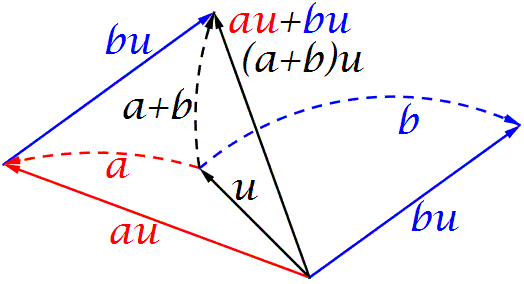
\includegraphics[width=0.5\textwidth]{imagenes/imagenes01/T01IM01.png}
		%\caption{Los dos problemas clásicos del cálculo: trazado de tangentes y áreas bajo curvas.}
	%\end{figure}
		
%varios párrafos encuadrados - explicaciones ad hoc
%\centering{
%\fbox{
%\parbox{0.95\textwidth}{
%varios
%
%$parrafos
%
%dentro
%}
%}
%}
% \justify


%\rotatebox{180}{\leftline{\textcolor{gris}{tararí}}}.

\chapter{Aplicaciones lineales $\divideontimes$}	


\section{Homomorfismos}	


El objetivo de este capítulo es el estudio de las aplicaciones lineales u homomorfismos entre espacios vectoriales. Este tipo de aplicaciones respeta la estructura de espacio vectorial transformando subespacios vectoriales en subespacios vectoriales. 


\begin{defi}
Sean $V \text{ y } V'$	dos subespacios vectoriales, una aplicación $f\,: \; V \; \to \; V'$ se dice que es una `aplicación lineal' u \emph{homomorfismo} si:

$\forall \vec u, \vec v \in V ; \; \forall \alpha, \beta \in \mathbb R \; : \quad $ \colorbox{LightYellow}{$\boxed{\; f\;(\;\alpha \vec u + \beta \vec v \; )= \alpha\; f(\vec u) + \beta \; f (\vec v)\; }$}
\end{defi}

\begin{ejem}.
	
\noindent --- $I:V\to V\; / \; I(\vec v)=\vec v,\; \forall \vec v \in V$ es, trivialmente, una aplicación lineal.

\noindent --- $f:\mathbb R^2 \to \mathbb R^3\; / \; f(x,y)=(x,x+y,x-2y)$ es una aplicación lineal:

\noindent $ f(\; \alpha(x_1,y_1)+\beta(x_2,y_2)\; )= f(\; \alpha x_1+\beta x_2\; , \; \alpha y_1+\beta y_2\; ) =$

\noindent $= (\; \alpha x_1 + \beta x_2 \; , \; \alpha x_1+\alpha y_1 + \beta x_2 + \beta y_2 \; , \; \alpha x_1+\beta x_2-2\alpha y_1 - 2 \beta y_2\; )=   $

\noindent $=\alpha\cdot (\; x_1, x_1+y_1, x_1-2y_1 \;)  +\beta \cdot (\; x_2, x_2+y_2, x_2-2y_2 \;) = $

\noindent $=\alpha \; f(x_1,y_1)+\beta \; f(x_2,y_2) $

\noindent --- $g:\mathbb R^2 \to \mathbb R^3 \; :\quad g(x,y)=(x^2, x+y,x-2y)$, no es una aplicación lineal pues (contraejemplo):

\noindent $g(\;(-1)\cdot (1,1) \;)= (1,-2,1); \quad (-1)\cdot g(1,1)=(-1)(1,2,-1)=(-1,-2,1) \Rightarrow g(\;(-1)\cdot (1,1) \;) \neq (-1)\cdot g(1,1)$

\noindent --- $h: \mathbb R^2 \to \mathcal M_{2 \times 2}(\mathbb R)\; : \quad h(x,y)=\left( \begin{matrix} x&0\\1&y \end{matrix} \right)$, no es una aplicación lineal.

\noindent $h(\; (x_1,y_1)+(x_2,y_2)\; )=\left( \begin{matrix} x _1+x_2&0\\1&y_1+y_2 \end{matrix} \right) \neq \left( \begin{matrix} x _1&0\\1&y_1 \end{matrix} \right) + \left( \begin{matrix} x_2&0\\1&y_2 \end{matrix} \right)=h(x_1,y_1)+h(x_2,y_2)$

\end{ejem}

Por su importante significado geométrico, destacamos \underline{algunas aplicaciones} \underline{lineales importantes}:

\begin{itemize}

\item \textbf{Aplicación identidad}: asigna a cada vector el mismo vector. 

$I:V\to V\;:\; I(\vec v)=\vec v$

\item \textbf{Aplicación nula}: siempre asocia el vector nulo del subespacio imagen.

$N:V \to V'\; :\; N(\vec v)=\vec 0_{V'}$

\item \textbf{Giros ángulo $\theta$}: Provoca un giro de $\theta$ grados sobre el vector.

$G_{\theta}: \mathbb R^2 \to \mathbb R^2 \; : \; G_{\theta} (x,y)= (\cos \theta \;x - \sin \theta \;y \;,\; \sin \theta \;x + \cos \theta \;y)$

\item \textbf{Reflexiones o simetrías}: un ejemplo de simetría en el espacio respecto del plano $XZ$ sería,

$S_{XZ}:\mathbb R^3 \to \mathbb R^3 \: :\; S_{_{XZ}}(x,y,z)=(x,-y,z)$

\item \textbf{Homotecias}: Producto de un escalar por un vector (si el escalar es, en módulo mayor que $1$ tenemos una dilatación; si es menor, una contracción). Como ejemplo pondremos la dilatación (superficial) de una lámina del $1\%$ debido al calor,

$D:\mathbb R^3 \to \mathbb R^3\; : \; D(x,y)=(1.01x, 1.01y)$

\item \textbf{Proyecciones}: Son aplicaciones que llevan todos los vectores de $\mathbb R^3$ a un plano sobre el que se proyecta. P.e., una proyección sobre el plano $YZ$ sería,

$P:\mathbb R^3 \to \mathbb R^3\; :\; P(x,y,z)=(x,0,z)$

\end{itemize}

\begin{defi}
Una aplicación lineal $\; f:V\to V'$ se dice que es:
\begin{itemize}
\item \textbf{inyectiva} si $\; f(\vec u)=f(\vec v) \longrightarrow \vec u = \vec v$, de otro modo, a originales distintos le corresponden imágenes distintas.
\item \textbf{epiyectiva, sobreyectica o suprayectica} si $\forall \vec v' \in V' \; \exists \vec v \in V\; / \; \vec v' = f(\vec v)$, es decir, si $f(V)=V'$
\item Si $f$ es inyectiva y epiyectiva se dice que es \textbf{biyectiva}	
\end{itemize}
	
\end{defi}

\begin{ejem}.

--- La aplicación del conjunto de la población española mayor de edad en $\mathbb N$ que asocia a cada ciudadano su DNI es INYECTIVA, pues no hay dos personas con el mismo DNI. Pero NO es EPIYECTIVA	porque no se usan todos los números naturales.

--- La aplicación de $\mathbb R$ en $\mathbb R^+$ que asocia a cada número real su cuadrado NO es INYECTIVA pues a los números opuestos les asocia en mismo cuadrado ($(2^2=(-2)^2=4$), pero sí es EPIYECTIVA ya que todos los números reales positivos son el cuadrado de algún número real.
\end{ejem}

\justify

Dependiendo de sus características las aplicaciones lineales (\textbf{homomor-fismos}) $f:V\to V'$ se clasifican en:

\begin{itemize}
\item MONOMORFISMO: si $f$ es inyectiva.
\item EPIMORFISMO: si $f$ es epiyectiva.
\item ISOMORFISMO: si $f$ es biyectiva.
\item ENDOMORFISMO: si $V=V'$
\item AUTOMORFISMO: si $V=V'$ y $f$ es biyectiva.
\end{itemize}

\section{Subespacios de una aplicación lineal.}

Las aplicaciones lineales transforman subespacios vectoriales en subsespacios vectoriales (conservan la estructura de subespacio vectorial):

\subsection{Subespacio \emph{Imagen} de una aplicación lineal}

\begin{prop}
$f:V\to V'$, sea $W \subseteq V$ un subespacio vectorial, entonces $f(W)=\{f(\vec u): \; \vec u\in W \}$	 es un subespacio vectorial de $V'$.
\end{prop}
\begin{proof}
\textcolor{gris}{ $\alpha, \beta \in \mathbb R; \; \vec u, \vec v \in f(W) \to \exists \vec u_1, \vec v_1 \in W \; / \; f(\vec u_1)=\vec u\; \wedge \; f(\vec v_1)=\vec v \Rightarrow \alpha\; \vec u + \beta\; \vec v = \alpha\; f(\vec u_1) + \beta\; f(\vec v_1) =f(\alpha\; \vec u_1+\beta \; \vec v_1)$, por lo que $ \alpha\; \vec u + \beta \; \vec v \in f(W)$ }	
\end{proof}

\begin{defi}
Dada $f:V\to V'$ aplicación lineal, se llama \textbf{imagen} de f, $\;Im(f)\;$, al conjunto $f(V)$ que, como se ha visto en la proposición anterior, es un subespacio vectorial de $V'$. Además, se cumple que: 

$f$ es \emph{epimorfismo} $\leftrightarrow Im(f)=V'$	 

------ La $Im(f)$ permite clasificar a los epimosfismos (aplicaciones epiyectivas o suprayectivas).
\end{defi}

\begin{ejem}
$f:\mathbb R^3 \to \mathbb R^3\;.\quad f(x,y,z)=(x+y,x-z,2x+y-z)$

\noindent $(x,y,z)\in Im(f) \text{ si } \exists (\alpha, \beta, \gamma)\in\mathbb R^3 \: : \quad (x,y,z)=f(\alpha, \beta, \gamma)=$

\noindent $=(\alpha+\beta, \alpha -\gamma, 2\alpha+\beta-\gamma)  \to \begin{cases} \alpha+\beta&=x\\ \alpha -\gamma&=y\\ 2\alpha+\beta-\gamma&=z \end{cases}$, ha de ser SC.

\noindent \textcolor{gris}{(\emph{ecuaciones paramétricas de $Im(f)$})}, calculando rangos por Gauss (p.e.):

\noindent \small{$\left( \begin{matrix} 1&1&0\\1&0&-1\\2&1&-1 \end{matrix} \right| \left. \begin{matrix} x\\y\\z \end{matrix} \right) \to  \left( \begin{matrix} 1&1&0\\0&-1&-1\\0&-1&-1 \end{matrix} \right| \left. \begin{matrix} x\\y-x\\z-2x \end{matrix} \right) \to \left( \begin{matrix} \boxed{1}&\boxed{1}&0\\\boxed{0}&\boxed{-1}&-1\\0&0&0 \end{matrix} \right| \left. \begin{matrix} x\\y-x\\z-2-y \end{matrix} \right) $}

\noindent \normalsize{al} exigir que los rangos de matrices de coeficientes y ampliada sean iguales a $2:\qquad z-x-y=0\;$, por lo que:

 $Im(f)=\{\;\ (x,y,z)\in \mathbb R^3\; : \quad z-x-y=0 \; \}$ \textcolor{gris}{(\emph{ecuación implícita de $Im(f)$})}.
\end{ejem}

Veamos un método alternativo de calcular $Im(f)$:

\begin{prop}
Sean $f:V\to V'$, aplicación lineal y $B=\{ \vec u_1, \cdots , \vec u_n \}$ una base de $V$, entonces $f(B)$ es un sistema generador de $Im(f)$.
\end{prop}

\begin{proof}
\textcolor{gris}{ Sea $\vec v\in Im(f) \to \exists \vec u \in V\ \therefore \; \vec v=f(\vec u)$. Como $B$ es base de $V$, existen $\alpha_1, \cdots , \alpha_n \in \mathbb R \; / \; \vec v = f(\vec u)= f(\alpha_1\; \vec u_1 + \cdots + \alpha_n\; \vec u_n)=\alpha_1 f(\vec u_1)	+ \cdots + \alpha_n f(\vec u_n)$, por lo que $f(B)$ genera el subespacio imagen $Im(f)$.}
\end{proof}

\begin{ejem} Calculemos, de otro modo $Im(f)$ del ejemplo anterior:

\noindent $f:\mathbb R^3 \to \mathbb R^3\;.\quad f(x,y,z)=(x+y,x-z,2x+y-z)$

\noindent$C=\{\; (1,0,0),(0,1,0),(0,0,1) \;\}$ es la base canónica de $\mathbb R^3$, calculamos $f(C)=\{\; (1,1,2),(1,0,1),(0,-1,.1) \;\}$, 

\noindent entonces $Im(f)=\mathcal L(\; \{\; (1,1,2),(1,0,1),(0,-1,-1) \;\} \; )$, es decir,

\noindent $(x,y,z)\in Im(f) \leftrightarrow \exists \; \alpha, \beta, \gamma \in \mathbb R\; \therefore \;$ 

\noindent $ (x,y,z)= \alpha (1,1,2)+ \beta (1,0,1) + \gamma (0,-1,-1)= (\alpha+\beta , \alpha-\gamma, 2\alpha+\beta-\gamma)$, que son las ecuaciones paramétricas de $Im(f)$ obtenidas en el ejemplo anterior. Si eliminamos los parámetros, como allí, obtendríamos:

\noindent  $z-x-y=0$ como ecuación implícita de $Im(f)$.
	
\end{ejem}



\subsection{Subespacio \emph{Núcleo} de una aplicación lineal}

\begin{defi}
Sea $f:V \to V'$ una aplicación lineal, se llama \textbf{núcleo}	 de f, $ker(f)$ \textcolor{gris}{ (de `kernel', de la raíz germánica Kern, núcleo) }, a los vectores de $V$ cuya imagen por $f$ es el $\vec 0 \;\in V':$

$Ker(f)=\{\; \vec u \in V \; : \; f(\vec u)=\vec 0 \textcolor{gris}{\; \in V'} \;\}$

\end{defi}

\begin{prop}
El núcleo de una aplicación lineal $f:V \to V'$, $\;\ker(f)\;$,	es un subespacio vectorial de $V$
\end{prop}
\begin{proof}
\textcolor{gris}{$\alpha, \beta \in \mathbb R; \; \vec u, \vec v \in ker(f): \; f(\vec u)=f(\vec v)=0 \to $}

\noindent \textcolor{gris}{$f(\alpha \vec u + \beta \vec v)=\alpha f(\vec u)+ \beta f(\vec v)  = \alpha \; \vec 0 + \beta \vec 0=\vec 0 \Rightarrow  (\alpha \vec u + \beta \vec v)\; \in ker(f)$}
\end{proof}

------ El núcleo permite caracterizar a los monomorfismos (aplicaciones inyectivas).

\begin{prop}
	Sea $f:V\to V'$ aplic. lineal. 
	
	Entonces, $f$ es inyectiva $\leftrightarrow Kerf(f)=\vec 0$
\end{prop}
\begin{proof}
\textcolor{gris}{ f inyectiva $\to  \vec u \in ker(f):\; f(\vec u)=\vec 0=f(\vec 0)$ y por inyectividad, $\vec u = \vec 0 \to Ker(f)=\{ \vec 0 \} $. Recíprocamente, si $Ker(f)=\{\vec 0 \} \text { y } f(\vec u)=f(\vec v),$ por linealidad, $\vec 0= f(\vec u)-f(\vec v)=f(\vec u - \vec v) \to \vec u-\vec v \in Kerf(f)=\{\vec 0\} \to \vec u=\vec v$  }	
\end{proof}

\begin{teor}
Sea $f:V \to V'$ una aplicación lineal de un espacio vectorial $V$ de dimensión finita en un espacio vectorial $V'$, se verifica la igualdad:

\begin{equation*}
	\colorbox{LightYellow}{\boxed{ \; dim(V)\; =\; dim \; Kem(f)\; +\; dim \; Im(f)\; }}
\end{equation*}	
\end{teor}

\begin{ejem}
$f:\mathbb R^3 \to 	\mathbb R^3\; : \quad f(x,y,z)=(x-y,x-z,-y-z)$. Calcula su núcleo y si imagen.

\noindent $(x,y,z) \in Ker (f) \leftrightarrow (0,0,0)= f(x,y,z)=(x-y,x-z,-y-z) \to \begin{cases} x-y=0 \\ x-z=0 \\ -y-z=0 \end{cases} \to SCD \text{ homog.} \to x=y=z=0 \Rightarrow $

\noindent $Ker(f)=\{(0,0,0\} \text{ y } dim\; ker(f)=0 \to dim\; Im(f)=3 \Rightarrow Im(f)=\mathbb R^3$
\end{ejem}

\section{Matriz asociada a una aplicación lineal}

Sea $f:V\to V'$ una aplicación lineal y sen $B=\{ \vec u_1, \cdots, \vec u_m \} $ y $B'=\{ \vec v_1, \cdots, \vec v_n \} $ dos bases de $V$ y $V'$ respectivamente. Dado un vector cualquiera $\vec u\in V$, existen $m$ escalares $\alpha_1, \cdots, \alpha_m \in \mathbb R$ de forma que: $\vec u = \alpha_1\; \vec u_1 + \cdots + \alpha_m\; \vec u_m$ \textcolor{gris}{(Estos $\alpha_i; \; 1\le i \le m$ son las componentes de $\vec u$ en la base $B$)} y por linealidad de $f$ tenemos que: 

$f(\vec u)=\alpha_1\cdot f(\vec u_1) + \cdots + \alpha_m\cdot f(\vec u_m)$

De donde se deduce que conociendo las imágenes por una aplicación lineal de ls vectores de una base del espacio inicial, es posible calcular la imagen que se obtiene por la aplicación lineal de cualquier vector. Por otra parte, $f(\vec u_1), \cdots, f(\vec u_m)$ estan en $V'$, por lo que pueden escribirse como combinación lineal de los vectores de una de sus bases, $B'$. Sean $\lambda_{1j}, \cdots, \lambda_{nj}\; \in \mathbb R$ las coordenadas de $f(\vec u_j)$ en $B'$, es decir,

$f(\vec u_j)=\lambda_{1j}\cdot f(\vec v_1) + \cdots + \lambda_{nj}\cdot f(\vec v_n)\; , \quad 1\le j \le m$, se tiene:

$\displaystyle f(\vec u)= \sum_{j=1}^m \alpha_{j}\cdot f(\vec u_j)=\sum_{j=1}^m \alpha_j \left( \sum_{i=1}^n \lambda_{ij}\cdot \vec v_i \right)=\sum_{i=1}^n \left( \sum_{j=1}^m \lambda_{ij} \; \alpha_j \right) \; \vec v_i$
 
 Si $\beta_1, \cdots, \beta_n\; \in \mathbb R$ son las componentes del vector $f(\vec u)$ en la base $B'$, como se trata de una base y un vector se escribe en ella de farma única:
 
 $\displaystyle \beta_i=\sum_{j=1}^m \lambda_{ij} \; \alpha_j \; , \quad 1\le i \le n\; $, matricialmente:
 
 $M_{BB'}(f)= \left(  \begin{matrix}  \lambda_{11} &  \lambda_{12}& \cdots &  \lambda_{1m} \\  \lambda_{21}& \lambda_{22}&\cdots & \lambda_{2m}\\ \vdots & \vdots & \ddots & \vdots \\  \lambda_{n1}& \lambda_{n2}&\cdots&  \lambda_{nm} \end{matrix}  \right)\; \in\; \mathcal M_{n \times m} (\mathbb R)$ , 
 
 cuyas columnas son las componentes en $B'$ de las imágenes por $f$ de los vectores $f(\vec u_i)$, con lo que:
 
 $\left( \begin{matrix} \beta_1 \\ \beta_2 \\ \vdots \\ \beta_n \end{matrix} \right) =   \left(  \begin{matrix}  \lambda_{11} &  \lambda_{12}& \cdots &  \lambda_{1m} \\  \lambda_{21}& \lambda_{22}&\cdots & \lambda_{2m}\\ \vdots & \vdots & \ddots & \vdots \\  \lambda_{n1}& \lambda_{n2}&\cdots&  \lambda_{nm} \end{matrix}  \right) \cdot \left( \begin{matrix} \alpha_1 \\ \alpha_2 \\ \vdots \\ \alpha_m \end{matrix} \right)$
 
 La matriz $M_{BB'}f$ es la \textbf{matriz de la aplicación $\boldsymbol{f}$ en las bases $\boldsymbol{B}$ y $\boldsymbol{B'}$} y permite obtener en la base $B'$ la imagen por $f$ de cualquier vector a partir de sus componentes es la base $B$, como se indica en la relación anterior.
 
 \begin{ejem}
 	Sean $f:\mathbb R^2 \to \mathbb R^3\; : \quad f(x,y)=(x,x+y.x-2y)$, una aplicación lineal; $\; C_2,\; C_3$ las bases canónicas de $\mathbb R^2 \text{ y } \mathbb R^3$.
 	
 \noindent $f(1,0)=(1,1,1); \quad f(0,1)=(0,1,-2) \quad \Rightarrow \quad\left( \begin{matrix} 1&0\\1&1\\1&-2 \end{matrix} \right)=M_{C_3C_2}(f)$ 
 	
 \noindent Consideremos $B=\{\; (1,1),(1,-1) \;\}$ una nueva base en $\mathbb R^2$, entonces:
 
 \noindent $\begin{cases} f(1,1)&=(1,2,-1)\\f(1,-1)&=(1,0,3) \end{cases} \quad \Rightarrow \quad \left( \begin{matrix} 1&1\\2&0\\-1&3 \end{matrix} \right)=M_{C_3B}(f)$
 
 \noindent Consideremos una nueva base en $\mathbb R^3,\quad B'=\{\; (1,0,0), (1,1,0), (1,1,1) \;\}$
 
 \noindent Es fácil comprobar (* ver más adelante, en gris) que: 
 
 \noindent $\begin{cases} f(1,1)=(1,2,-1)_{C_3}=(-1,3,-1)_{B'}\\ f(1,-1)=(1,0,3)_{C_3}=(1,-3,3)_{B'} \end{cases} \quad \Rightarrow \quad \left( \begin{matrix} -1&1\\3&-3\\-1&3 \end{matrix} \right)=M_{B'B}(f)$
 
 \end{ejem}

\textcolor{gris}{Como se vio en el apartado de matriz cambio de base en el tema de espacios vectoriales, ver sección \ref{matriz-cambio-base}, se tiene que (ahora con vectores columnas usamos las matrices traspuestas de las que allí se vieron):}
 
 \textcolor{gris}{$\vec w_C = M_{BC}\cdot \vec w_B \quad \to \quad  \left( \begin{matrix} 1\\2\\-1 \end{matrix} \right)= \left( \begin{matrix} 1&1&1\\0&1&1\\0&0&1 \end{matrix} \right) \cdot \left( \begin{matrix} \alpha\\ \beta\\ \gamma \end{matrix}\right) $ }
 
 \textcolor{gris}{de donde: $\begin{cases} 1=\alpha+\beta+\gamma\\2=\beta+\gamma\\-1=\gamma \end{cases} \quad \to \quad \alpha=-1;\; \beta=3; \; \gamma=-1  $ }
 
 \textcolor{gris}{Es decir: $(1,2,-1)^T_C=(-1,3,-1)^T_{B'} \;$ y, del mismo modo, $(1,0,3)_C=(1,-3,3)^T_{B'} $}
 
 \textcolor{gris}{Hubiésemos podido usar la matriz inversa: $\boldsymbol{M^{-1}_{BC}} \cdot \vec w_C = \boldsymbol{M^{-1}_{BC}} \cdot M_{BC}\cdot \vec w_B \to \vec w_B =M_{CB}\cdot \vec w_C$, donde $M_{CB}=M^{-1}_{BC}$} 


\section{Ejercicios resueltos}

\begin{ejre}
Dada la aplicación lineal: $f:\mathbb R^3 \to \mathbb R^2\; : \; f(x,y,z)=(x+y-z,2x+3z)$, se pide:

a)  Probar que $f$ es una aplicación lineal.

b) Hallar su núcleo y su imagen.

c) Obtener la matriz asociada a $f$ en las bases canónicas de $\mathbb R^3 \text{ y } \mathbb R^2$	


\end{ejre}

\begin{proofw}\renewcommand{\qedsymbol}{$\diamond$}
	--- a) $\forall \vec u=(x,y,z);\; \vec v=(x',y',z')\in \mathbb R^3; \; \forall \alpha, \beta \in \mathbb R \;$, ¿es cierto que $  f(\alpha \vec u+\beta \vec v)=\alpha f(\vec u)+\beta f(\vec v)$

\noindent $f(\alpha \vec u+\beta \vec v)=f(\alpha x+\beta x', \alpha y+\beta y', \alpha z + \beta z')=\cdots $ (aplíquese la definición de $f$ y simplifíquese al máximo (*1).

\noindent  $\alpha f(\vec u)+\beta f(\vec v)=\alpha f(x,y,z)+\beta f(x',y'.z')=\cdots$  (aplíquese la definición de $f$ y simplifíquese al máximo (*2)

\noindent Compruébese, ahora, que (*1) y (*2) son el mismo resultado, por lo que $f$ sí es aplicación lineal.

\noindent --- b) $Ker(f)=\{(x,y,z)\; / \; f(x,y,z)=(0,0)\} \to \begin{cases} x+y-z=0\\2x+3z=0\end{cases} \;$, se trata de un SEL homogéneo que sale SCI:  $x=-3\lambda /2,\; y=5\lambda  /2, \; z=\lambda \;\, (\forall \lambda \in \mathbb R) \Rightarrow Ker(f)=\{\; (-3\lambda /2, 5\lambda  /2, \lambda),\;\; \forall \lambda \in \mathbb R \; \}$

\noindent Con $\lambda =2 \to (-3,5,2)$ es un sistema generador de $Ker(f)$ que, como es un solo vector LI se trata de una base: $B_{Kerf(f)}=\{(-3,5,2)\}$

\noindent --- c) Matriz asociada en las bases canónicas de los espacios vectoriales inicial y final sobre los que actúa $f$:

\noindent $\begin{cases} f(1,0,0)=(1,2)\\f(0,1,0)=(1,0)\\f(0,0,1)=(-1,3) \end{cases} \longrightarrow M_{C_2C_3}(f)=\left( \begin{matrix} 1&2\\1&0\\-1&3 \end{matrix} \right)$

\end{proofw}


\begin{ejre}
	Sea $(\mathcal P_2(x),+,\cdot)$ el espacio vectorial de los polinomios de segundo grado de una variable reales con la operación suma de polinomios y producto de un polinomio por un número usuales. Sea $f:\mathcal P_2(x) \to \mathcal P_1(x)$ la aplicación que a cada polinomio de segundo grado de $\mathcal P_2(x)$ le hace corresponder  su derivada, un polinomio de $\mathcal P_1(x)$: $\forall p(x)\in \mathcal P_2(x):\; f(p(x))=p'(x)$. Probar que se trata de una aplicación lineal, obtener su matriz asociada respecto de las bases canónicas  de $\mathcal P_2(x)$ y $\mathcal P_1(x)$ y  clasificarla.
\end{ejre}

\begin{proofw}\renewcommand{\qedsymbol}{$\diamond$}
	
	$f: \mathcal P_2(x) \to \mathcal P_1(x)\; :\; \; p(x) \rightsquigarrow p'(x) \; \therefore \; ax^2+bx+c \longrightarrow 2ax+b\,$, es decir, $f(ax^2+bx+c)=2ax+b$

\noindent \textcolor{gris}{\textbf{Linealidad:}} $f(\alpha p(x)+ \beta q(x))=f(\alpha (ax^2+bx+c)+\beta (a'x^2+b'x+c'))=f( (\alpha a + \beta a')x^2+(\alpha b + \beta b')x+(\alpha c+\beta c'))=2(\alpha a + \beta a')x+ (\alpha b + \beta b')$

\noindent por otro lado: $\alpha f(p(x))+\beta f(q(x))=\alpha f(ax^2+bx+c)+\beta (a'x^2+b'x+c)= 2\alpha a x+\alpha b+2\beta a' x+ \beta b'=2(\alpha a + \beta a')x+ (\alpha b + \beta b')$

\noindent Luego $f$ sí es aplicación lineal.

\noindent  \textcolor{gris}{\textbf{Matriz asociada:}} Sean $C_2=\{x^2,x,1\} \text{ y } C_1=\{x,1\}$ las bases canónicas de $\mathcal P_2(x)$ y $\mathcal P_1(x)$, respectivamente.

\noindent 

$ \begin{cases} \; f(x^2)=2x&=2\cdot x+ 0\cdot 1 \\
\; f(x)=1&=0\cdot x + 1 \cdot 1 \\ \; f(1)=0&=0\cdot x + 0 \cdot 0 \end{cases}  \quad \longrightarrow \quad M_{C_2C_1}(f)=\left( \begin{matrix} 2&0&0\\0&1&0 \end{matrix} \right)$

\noindent Modo de actuar:  $f(ax^2+bc+c)=\left( \begin{matrix} 2&0&0\\0&1&0 \end{matrix} \right) \cdot \left( \begin{matrix} a\\b\\c \end{matrix} \right)=\left( \begin{matrix} 2a\\b \end{matrix} \right)=2ax+b$

\noindent  \textcolor{DimGray}{\textbf{Clasificación:}} Núcleo e Imagen.

\noindent --- Núcleo: $f(ax^2+bx+c)=0x+0 \to a=b=0, \; \forall c$, luego $Ker(f)=\{(0,0,c),\; c\in \mathbb R \} \to B_{Ker(f)}=\{(0,0,1)\} \to dim \; Ker(f)=1$, como el núcleo no es $0x^2+0x+0$, la aplicación no es inyectiva.

\noindent --- Imagen: Las imágenes de una base del espacio inicial son un sistema generador del subespacio imagen $\to \{(2,0),(0,1),(0,0)\}$ es un sistema generador de $Im(f)$, los dos primeros vectores son LI (rango $2$), por lo que forman una base: $B_{Im(f)}=\{(2,0),(0,1))\} \to dim\; Im(f)=2$, igual al espacio de llegada. La aplicación es suprayectiva o epiyectiva.

\noindent Conclusión: $f$ es un ` EPIMORFISMO', aplicación suprayectiva.
	
\end{proofw}


\begin{ejre}
	$f:\mathbb R^2 \to \mathcal M_2(R) \: \quad f(x,y)=\left( \begin{matrix} x&x+y\\0&y \end{matrix} \right)$
	
	Compruébese que es lineal, Calcúlese Núcleo e Imagen, clasifíquese y encuéntrese la matriz asociada a $f$ en las bases canónicas de $\mathbb R^2 \text{ y } \mathcal M_2(R)$.
\end{ejre}

\begin{proofw}\renewcommand{\qedsymbol}{$\diamond$}
	
\noindent \textcolor{gris}{\textbf{Linealidad:}} $f(\alpha(x,y)+\beta(x',y'))=\left( \begin{matrix} \alpha x+\beta x'&\alpha x+\beta x'+ \alpha y+\beta y'\\0&\alpha y+\beta y' \end{matrix} \right)$

\noindent $\alpha f(x,y)+\beta f(x',y') = \alpha \left( \begin{matrix} x&x+y\\0&y \end{matrix} \right)+ \beta \left( \begin{matrix} x'&x'+y'\\0&y' \end{matrix} \right)$

\noindent como ambos resultados obviamente coinciden, $f$ sí es aplicación lineal.

\noindent \textcolor{gris}{\textbf{Núcleo e Imagen:}} 

\noindent --- Núcleo: $\; Ker(f)=\left\{(x,y)\in \mathbb R^2\; / \; \left( \begin{matrix} x&x+y\\0&y \end{matrix} \right)=\left( \begin{matrix} 0&0\\0&0 \end{matrix} \right) \right\} \to $

\noindent \small{$\begin{cases} x=0\\x+y=0\\y=0 \end{cases} \to x=y=0 \Rightarrow Ker (f)=\{(0,0)\}=\vec 0_{\mathbb R^2} \to dim\; Ker (f)=0$}

\noindent \normalsize{--- Imagen:} $f(x,y)=\left( \begin{matrix} x&x+y\\0&y \end{matrix} \right)= x \; \left( \begin{matrix} 1&1\\0&0 \end{matrix} \right) + y \; \left( \begin{matrix} 0&1\\0&1 \end{matrix} \right) \to Im(f)= \mathcal L \left\{\;  \left( \begin{matrix} 1&1\\0&0 \end{matrix} \right)\; , \; \left( \begin{matrix} 0&1\\0&1 \end{matrix} \right)\;  \right\} =$ sistema generador de $Im(f)$ donde es fácil probar que son dos vectores (matrices) LI, por lo que forman una base y $B_{Im(f)}= \left\{\;  \left( \begin{matrix} 1&1\\0&0 \end{matrix} \right)\; , \; \left( \begin{matrix} 0&1\\0&1 \end{matrix} \right)\;  \right\} \to dim \; Im(f)=2$

\noindent \textcolor{gris}{\textbf{ Clasificación:}} Como $dim\; Ker(f)=0\; f \, $ es inyectiva y como $\dim \; Im(f)=2\neq 4 = dim\; \mathcal M_2(\mathbb R)$, por ello, $f$ no es supreyectiva o epiyectiva. 

\noindent Conclusión: f es un `MONOMORFISMO', aplicación lineal inyectiva.

\noindent \textcolor{gris}{\textbf{ Matriz asociada a $f$:}}

\noindent $B_{\mathbb R^2}= \{ \; (1,0)\;,\;(0,1\;\}$

\noindent $B_{\mathcal M_2(\mathbb R)}= \left\{
\left( \begin{matrix} 1&0\\0&0 \end{matrix} \right)\; , \;
\left( \begin{matrix} 0&1\\0&0 \end{matrix} \right)\; , \;
\left( \begin{matrix} 0&0\\1&0 \end{matrix} \right)\; , \;
\left( \begin{matrix} 0&0\\0&1 \end{matrix} \right) \;
\right\}$

\noindent $f(1,0)=\left( \begin{matrix} 1&1\\0&0 \end{matrix} \right) =
1\cdot \left( \begin{matrix} 1&0\\0&0 \end{matrix} \right)+
1 \cdot \left( \begin{matrix} 0&1\\0&0 \end{matrix} \right)+
0 \cdot \left( \begin{matrix} 0&0\\1&0 \end{matrix} \right)+
0 \cdot \left( \begin{matrix} 0&0\\0&1 \end{matrix} \right) $

\noindent $f(0,0)=\left( \begin{matrix} 0&1\\0&1 \end{matrix} \right) =
0\cdot \left( \begin{matrix} 1&0\\0&0 \end{matrix} \right)+
1 \cdot \left( \begin{matrix} 0&1\\0&0 \end{matrix} \right)+
0 \cdot \left( \begin{matrix} 0&0\\1&0 \end{matrix} \right)+
1 \cdot \left( \begin{matrix} 0&0\\0&1 \end{matrix} \right) $

\noindent por lo que: $\; \; M_{\mathcal M_2 \mathbb R^2}= \left( \begin{matrix} 1&0\\1&1\\0&0\\0&1 \end{matrix} \right)$

\noindent \textcolor{gris}{Funcionamiento de la matriz: por ejemplo,}

\noindent \textcolor{gris}{$f(1,3)=\left( \begin{matrix} 1&0\\1&1\\0&0\\0&1 \end{matrix} \right)\cdot \left( \begin{matrix} 1\\3 \end{matrix} \right)= \left( \begin{matrix} 1\\4\\0\\3 \end{matrix} \right) = 
\boldsymbol{1} \cdot \left( \begin{matrix} 1&0\\0&0 \end{matrix} \right)+
\boldsymbol{4} \cdot \left( \begin{matrix} 0&1\\0&0 \end{matrix} \right)+
\boldsymbol{0} \cdot \left( \begin{matrix} 0&0\\1&0 \end{matrix} \right)+
\boldsymbol{3} \cdot \left( \begin{matrix} 0&0\\0&1 \end{matrix} \right)=
\left( \begin{matrix} 1&4\\0&3 \end{matrix} \right)$}

\end{proofw}


\begin{ejre}
	Dada la aplicación lineal $f:\mathbb R^3 \to \mathbb R^3\; :\; \; f(x,y,z)=(x+y,y-z,x+y+z)$, calcúlese su núcleo, imagen y clasifíquese.
\end{ejre}

\begin{proofw}\renewcommand{\qedsymbol}{$\diamond$}
	--- Núcleo: $Ker (f)=\{(x,y,z)\; / \;f(x,y,z)=(x+y,y-z,x+y+z)=(0,0,0) \} \to$ formal un SEL que es SCD y homogéneo (compruébese), por lo que $Ker f=\{(0,0,0)\}=\{ \vec 0\} \to dim \; Ker(f)=0$ y la aplicación lineal será `inyectiva'.
	
\noindent --- Imagen: $f(x,y,z)=(x+y,y-z,x+y+z)=x\cdot (1,0,1)+y \cdot (1,1,1)+ z\cdot (0,-1,1) \to Im(f)=\mathcal L \left\{\; (1,0,1), (1,1,1), (0,-1,1) \right\}$ que es fácil comprobar que forman un sistema libre o LI (compruébese), por lo que $dim\; im(f)=3=\dim(\mathbb R^3)$ y tendremos una aplicación `epiyectiva'.

\noindent--- Clasificación: por lo visto en los apartados anteriores, $f$ es una aplicación biyectiva u `ENDOMORFISMO'

\noindent \textcolor{gris}{Como $\begin{cases} f(1,0,0)=(1,0,1)\\f(0,1,0)=(1,1,1)\\f(0,0,1)=(0,-1,1) \end{cases} \to \quad M_{C_3C_3}(f)= \left( \begin{matrix} 1&1&0\\0&1&-1\\1&1&1 \end{matrix} \right)$ es la matriz canónica del endomorfismo $f$.}
\end{proofw}



\begin{myexampleblock}{Aplicación lineal u HOMOMORFISMO}

Una gran cantidad de modelos de la ingeniería siguen leyes `lineales'. Podemos imaginarnos un aparato que cada vez que se le introduce un determinado estímulo devuelve ese estímulo modificado como una señal de salida. Dicho estímulo puede ser por ejemplo una diferencia de potencial de potencial en un circuito eléctrico que a su vez devolverá una cierta intensidad de corriente. Si denotamos por $V (t)$ el voltaje e $I(t)$ la intensidad, el circuito funciona de la manera siguiente: si $I_1(t)$ e $I_2(t)$ son las respuestas a los voltajes $V_1(t)$ y $V_2(t)$, entonces $I_1(t) + I_2(t)$ es la respuesta al voltaje $V_1(t) + V_2(t)$.  Además, si el voltaje es amplificado multiplicando por un escalar $\alpha$, entonces $\alpha \;I(t)$ es la respuesta a $\alpha \; V (t)$. Esta es la forma de funcionar de un circuito \textbf{LRC} y la de numerosos ingenios de la ingeniería, estos aparatos funcionan como una aplicación lineal u \emph{homomorfismo}. 

\end{myexampleblock}



	%\begin{figure}[H]
		%\centering
		%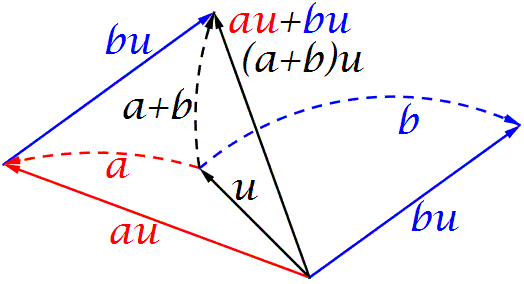
\includegraphics[width=0.5\textwidth]{imagenes/imagenes01/T01IM01.png}
		%\caption{Los dos problemas clásicos del cálculo: trazado de tangentes y áreas bajo curvas.}
	%\end{figure}
		
%varios párrafos encuadrados - explicaciones ad hoc
%\centering{
%\fbox{
%\parbox{0.95\textwidth}{
%varios
%
%$parrafos
%
%dentro
%}
%}
%}
% \justify


%\rotatebox{180}{\leftline{\textcolor{gris}{tararí}}}.

\chapter{Diagonalización de matrices  $\divideontimes$}	


	

\section{Valores y vectores prropios}

Los conceptos de valores y vectores propios cuestan un poco de entender, veamos su definición.

\begin{defi}
Los \textbf{`vectores propios o autovectores'} son los vectores no nulos de una aplicación lineal que, cuando son transformados por ella, dan lugar a un múltiplo escalar de ellos (no cambian de dirección). Este escalar el el \textbf{`valor propio o autovalor'}:

\vspace{4mm}\centerline{\colorbox{LightYellow}{$\boldsymbol{\; A\; \vec v = \lambda \; \vec v  \;,}$}}

\justify
donde $A$ es la matriz de la aplicación lineal, $\vec v$ es el vector propio y $\lambda$ el valor propio o característico. Hay quien usa la raíz alemana y habla de `eigen-valores' y `eigen-vectores'.

\end{defi}

Para el cálculo de los valores y vectores propios de una matriz (aplicación lineal) se sigue el siguiente \emph{`algoritmo'}:

\begin{enumerate}
\item Calcular la `ecuación característica': $\quad det(A-\lambda I)$
\item Encontrar las raíces del `polinomio característico' obtenido: 

$ det(A-\lambda I)=0 \longrightarrow \lambda_i$. Estos son los valores propios.

\item Calcular el vector propio correspondiente a cada uno de los valores propios obtenidos en el paso anterior:	

$A\vec v=\lambda \vec v \to (A-\lambda  I)\vec v=\vec 0$
\end{enumerate}

Para el cálculo de los valores y vectores propios de una matriz también es conveniente tener en cuenta los siguientes `trucos' \textcolor{gris}{(proposiciones que no vamos a demostrar)}.

\begin{itemize}
\item La traza de una matriz A (suma de los elementos de su diagonal principal)	coincide con la suma de los autovalores o valores propios:

$\displaystyle tr(A)=\textcolor{gris}{\sum_{i=1}^n a_{ii}}=\sum_{i=1}^n \lambda_i$

\item El producto de todos los valores propios coincide con el determinante de la matriz.

$\displaystyle det(A)=\prod_{i=1}^n \lambda_i$

\item Si hay una combinación lineal en filas o columnas de $A$, entonces un valor propio, al menos, de la matriz es cero.
\end{itemize}

\begin{ejem}
Dada $A=\left( \begin{matrix} 1&0\\5&2 \end{matrix} \right)$, encuentra sus autovalores y autovectores.

$det(A-\lambda I)=\left| \begin{matrix} 1-\lambda&0\\5&2-\lambda \end{matrix} \right|=\lambda^2-3\lambda+2=0 \longrightarrow \lambda =1 \; \wedge \; \lambda=2$

--- $\lambda =1 \longrightarrow (A-\lambda I)\vec v=\vec 0 \to (A-I)\vec v=\vec 0\to (A-I)\left( \begin{matrix} x\\y \end{matrix} \right) = \left( \begin{matrix} 0\\0 \end{matrix} \right)$ 

\noindent \small{$\left( \begin{matrix} 0&0\\5&1 \end{matrix} \right)\left( \begin{matrix} x\\y \end{matrix} \right) = \left( \begin{matrix} 0\\0 \end{matrix} \right) \to \begin{cases} 0x+0y=0\\5x+y=0 \end{cases} \to y=-5x \Rightarrow (x=1)\; 
\vec v=\left( \begin{matrix} 1\\-5 \end{matrix} \right)$}\normalsize{.}


--- $\lambda =2 \longrightarrow (A-\lambda I)\vec v=\vec 0 \to (A-2I)\vec v=\vec 0\to (A-2I)\left( \begin{matrix} x\\y \end{matrix} \right) = \left( \begin{matrix} 0\\0 \end{matrix} \right)$	

\noindent \small{ $\left( \begin{matrix} -1&0\\5&0 \end{matrix} \right)\left( \begin{matrix} x\\y \end{matrix} \right) = \left( \begin{matrix} 0\\0 \end{matrix} \right) \to \begin{cases} -x+0y=0\\5x+0y=0 \end{cases} \to x=0 \Rightarrow (y=1)\; 
\vec v=\left( \begin{matrix} 0\\1 \end{matrix} \right)$}\normalsize{.}

Conclusión, los valores propios y sus correspondientes valores propios de la matriz A son:

$\lambda=1 \leftrightarrow \vec v=\left( \begin{matrix} 1\\-5 \end{matrix} \right)
\quad; \qquad \qquad  
\lambda = 2 \leftrightarrow \vec v=\left( \begin{matrix} 0\\1 \end{matrix} \right)$
\end{ejem}


\section{Diagonalización de matrices}

\begin{defi}
Una \textbf{matriz diagonalizable} es una matriz cuadrada que se puede transformar en una matriz diagonal.	

La diagonalización de las matrices es del siguiente modo:

\vspace{4mm} \centerline{\colorbox{LightYellow}{$\boxed{ \; \boldsymbol{A=PDP^{-1} \quad \leftrightarrow \quad D=P^{-1}AP}\; }$ ,}}

\justify

donde $A$ es la matriz a diagonalizar, $P$ es la matriz formada por los vectores propios de $A$ escritos como columnas, $P^{-1}$ es la matriz inversa de $P$ y $D$ es la matriz diagonalizada, cuyos elementos de la diagonal principal son los autovalores de $A$. \textcolor{gris}{La matriz $P$ actúa como una matriz de cambio de base, por lo que, en realidad, con esta fórmula estamos cambiando la matriz $A$ a una nueva base en que se convierte en diagonal $D$. Evidentemente, $P$ es una matriz regular o invertible.} 
\end{defi}

No todas las matrices son diagonalizables, tan solo se pueden diagonalizar las matrices que cumplen con unas ciertas características. Se puede saber si una matriz es diagonalizable de distintas maneras:

\begin{itemize}

\item Una matriz cuadrada de orden $n$ es diagonalizable si tiene $n$ vectores propios (o autovectores) linealmente independientes, o dicho de otra forma, si estos vectores forman una base. Eso es debido a que la matriz $P$, que sirve para diagonalizar la matriz dada $A$, está formada por los vectores propios de dicha matriz $A$. Para saber si los autovectores son LI, basta con que el determinante de la matriz $P$ sea diferente de $0$, cosa que significa que la matriz es de rango máximo. $\quad$ \emph{Si $det(P)\neq 0 \to $ matriz diagonalizable.}
\item Una propiedad de los valores y vectores propios es que los autovectores de autovalores diferentes son linealmente independientes. Por lo tanto, si todos los autovalores de la matriz son únicos (todos tienen multiplicidad uno)  la matriz es diagonalizable.
\item Finalmente, existe un teorema, el \emph{`teorema espectral'}, que garantiza la diagonalización de las matrices simétricas con números reales. Es decir, \emph{toda matriz real y simétrica es diagonalizable}.
	
\end{itemize}

Para diagonalizar  una matriz (aplicación lineal) $A$ se sigue el siguiente \emph{`algoritmo'}:

\begin{enumerate}
\item Obtener los valores ($\lambda_i$)y vectores propios ($\vec v_i$) de $A$
\item Construir la matriz $P$ formada los los vectores-columna propios de $A$
\item Verificar que $A$ es digonalizable, está en alguno de los supuestos anteriores.
\item Construir la matriz $D$ en que todos sus elementos son cero excepto los de la diagonal principal, que son los valores propios de $A$:

$D=(d_{ij})=\begin{cases} \lambda_i & \text{ si } i=j \\
0 & \text{ si } i \neq j \end{cases}$	
\end{enumerate}

NOTA: Los vectores propios en $P$ se pueden escribir en cualquier orden, pero entonces, hay que respetar ese mismo orden al escribir los valores propios en $D$: 

$P=\left( \vec v_1 \; | \; \vec v_2 \; | \; \cdots \; | \; \vec v_n \right) \longrightarrow D=\left( \begin{matrix} \lambda_1 &0&\cdots &0 \\ 0&\lambda_2&\cdots & 0 \\ \vdots & \vdots & \ddots & \vdots \\ 0&0&\cdots & \lambda_n \end{matrix} \right)$

\begin{teor}{Aplicaciones de las matrices diagonalizables}
Al estar las matrices diagonales llenas de ceros el cálculo se simplifica muchísimo. Un ejemplo claro de ellos son las `potencias' de las matrices cuadradas:

\vspace{4mm} \centerline{\colorbox{LightYellow}{$\; A^k=PD^kP^{-1} \; , \qquad D^k=diag(\lambda_1^k, \lambda_2^k, \cdots, \lambda_n^k)\; $	}}
\end{teor}
\begin{proofw}

\textcolor{gris}{\noindent $A^2=A\cdot A = (PDP^{-1})\cdot  (PDP^{-1})= PD\; P^{-1} P\; DP^{-1}=  PDIDP^{-1}=PD^2P$}

\noindent \textcolor{gris}{\noindent $A^3=A^2\cdot A= (PD^2P^{-1})\cdot (PDP^{-1})=PD^2\;P^{-1})P\; DP^{-1}=PD^2IDP^{-1}=PD^3P$}

\noindent \textcolor{gris}{\noindent . . . . . . . . . . . . . . . .}

\noindent \textcolor{gris}{\noindent Conjeturamos: $A^k=PD^kP$, necesitaría de una demostración por inducción que de le deja al lector.}
	
\end{proofw}
	



\begin{ejem}
Diagonaliza la matriz $A=\left( \begin{matrix} 2&2\\1&3 \end{matrix} \right)$

$|A-\lambda I|=\left| \begin{matrix} 2-\lambda&2\\1&3-\lambda \end{matrix}  \right|=\lambda^2-5\lambda +4=0 \leftrightarrow \lambda_1=1; \; \wedge \; \lambda_2=4	$

--- $ \lambda=1 \to (A-I)\vec v= \vec 0 \to \left( \begin{matrix} 1&2\\1&2 \end{matrix} \right)\; \left( \begin{matrix} x\\y \end{matrix} \right)=
\left( \begin{matrix} 0\\0 \end{matrix} \right)$

$\begin{cases} x+2y=0\\x+2y=0 \end{cases} \to x=-2y \Rightarrow \vec v_1=\left( \begin{matrix} -2\\1 \end{matrix} \right)$

--- $ \lambda=4 \to (A-4I)\vec v= \vec 0 \to \left( \begin{matrix} -2&2\\1&-1 \end{matrix} \right)\; \left( \begin{matrix} x\\y \end{matrix} \right)=
\left( \begin{matrix} 0\\0 \end{matrix} \right)$

$\begin{cases} -x+2y=0\\x-y=0 \end{cases} \to x=y \Rightarrow \vec v_2=\left( \begin{matrix} 1\\1 \end{matrix} \right)$

Por lo que: $\quad P=\left( \begin{matrix} -2&1\\1&1 \end{matrix} \right) \quad , \qquad \qquad 
D=\left( \begin{matrix} 1&0\\0&4 \end{matrix} \right) $

\noindent \footnotesize{\textcolor{gris}{Compruébese que $D=P^{-1}AP \to  \left( \begin{matrix} 1&0\\0&4 \end{matrix} \right)=\left( \begin{matrix} -2&1\\1&1 \end{matrix} \right)^{-1} \cdot 
\left( \begin{matrix} 2&2\\1&3 \end{matrix} \right) \cdot 
\left( \begin{matrix} -2&1\\1&1 \end{matrix} \right)$ }}\normalsize{.}

\noindent \footnotesize{\textcolor{gris}{Así como que $A^4=PD^4P^{-1}=\left( \begin{matrix} 86&170\\85&171 \end{matrix} \right), \; con \; D^4=\left( \begin{matrix} 1^4&0\\0&4^4 \end{matrix} \right)=\left( \begin{matrix} 1&0\\0&256 \end{matrix} \right)$  }}\normalsize{.}


\end{ejem}







\section{Ejercicios resueltos}

\begin{ejre}.

Encuentra los autovalores y autovectores de $A=\left( \begin{matrix} 1&2&0\\2&1&0\\0&1&2 \end{matrix} \right)$	
\end{ejre}

\begin{proofw}\renewcommand{\qedsymbol}{$\diamond$}
	$|A-\lambda I|=\left| \begin{matrix} 1-\lambda &2&0 \\2&1-\lambda &0 \\0&1&2-\lambda \end{matrix} \right|=-\lambda^3+4\lambda^2-\lambda -6=$
	
\noindent $= -(\lambda-2)(\lambda-3)(\lambda+1)=0 \to \lambda=-1; \; \lambda=2;\; \lambda=3$

\noindent --- $\lambda=-1:\; (A+I)\vec v =\vec 0 \to \left( \begin{matrix} 2&2&0\\2&2&0\\0&1&3 \end{matrix} \right) \; \left( \begin{matrix} x\\y\\z \end{matrix} \right)=\left( \begin{matrix} 0\\0\\0 \end{matrix} \right)$

\noindent $\begin{cases} 2x+2y=0\\2x+2y=0\\y+3z=0 \end{cases} \to x=-y \; y=-3z \to \vec v_{-1}= \left( \begin{matrix} 3\\-3\\1 \end{matrix} \right)$


\noindent --- $\lambda=2:\; (A-2I)\vec v =\vec 0 \to \left( \begin{matrix} -1&2&0\\2&-1&0\\0&1&0 \end{matrix} \right) \; \left( \begin{matrix} x\\y\\z \end{matrix} \right)=\left( \begin{matrix} 0\\0\\0 \end{matrix} \right)$

\noindent $\begin{cases} -x+2y=0\\2x-y=0\\y=0 \end{cases} \to x=y=0 \to \vec v_{2}= \left( \begin{matrix} 0\\0\\1  \end{matrix} \right)$


\noindent --- $\lambda=3:\; (A-3I)\vec v =\vec 0 \to \left( \begin{matrix} -2&2&0\\2&-3&0\\0&1&-1 \end{matrix} \right) \; \left( \begin{matrix} x\\y\\z \end{matrix} \right)=\left( \begin{matrix} 0\\0\\0 \end{matrix} \right)$

\noindent $\begin{cases} -2x+2y=0\\2x-2y=0\\y-z=0 \end{cases} \to x0y=z \to \vec v_{3}= \left( \begin{matrix} 1\\1\\1 \end{matrix} \right)$

\end{proofw}


\begin{ejre}.

	$A=\left( \begin{matrix} 1&0&-1&0\\2&-1&-3&0\\-2&0&2&0\\0&0&0&3 \end{matrix} \right)$. Encuentra sus autovalores y autovectores
\end{ejre}

\begin{proofw}\renewcommand{\qedsymbol}{$\diamond$}
	$|A-\lambda I|=0 \leftrightarrow \lambda =0,\; \lambda =-1, \; \lambda=3 \; \text{, raíz doble }$
	
\noindent --- $\lambda = 0 \to (A-0I)\vec v=\vec 0 \to x=-y=z; \; t=0 \to \vec v_{0}= \left( \begin{matrix} 1\\-1\\1\\0 \end{matrix} \right)$

\noindent --- $\lambda = -1 \to (A+I)\vec v=\vec 0 \to x=z=0; \; t=0 \to \vec v_{-2}= \left( \begin{matrix} 0\\1\\0\\0 \end{matrix} \right)$

\noindent --- $\lambda = 3 \to (A-3I)\vec v=\vec 0 \to y=2x; \; z=-2x \to $

\noindent Autovalor doble, dos autovectores: $\vec v_{3_1}= \left( \begin{matrix} 1\\2\\-2\\0 \end{matrix} \right)\;; \; \;\;  \vec v_{3_2}= \left( \begin{matrix} 0\\0\\0\\1 \end{matrix} \right)$
\end{proofw}


\begin{ejre}
	Diagonaliza $A=\left(\begin{matrix} 2&0&2\\-1&2&1\\0&1&4  \end{matrix}\right)$
\end{ejre}

\begin{proofw}\renewcommand{\qedsymbol}{$\diamond$}.

\noindent \small{$ \lambda_1=1 \longrightarrow \vec v_1=\left( \begin{matrix} -2\\-3\\1 \end{matrix}\right); \; \lambda_2=3 \longrightarrow \vec v_2=\left( \begin{matrix} 2\\-1\\1 \end{matrix}\right); \;\lambda_3=4 \longrightarrow \vec v_3=\left( \begin{matrix} 1\\0\\0 \end{matrix}\right)$}\normalsize{.}

$P=\left(\begin{matrix} -2&2&1\\-3&1&0\\1&1&1  \end{matrix}\right); \qquad D=\left(\begin{matrix} 1&0&0\\0&3&0\\0&0&4  \end{matrix}\right)$

\end{proofw}
	
\begin{ejre}
	Diagonaliza $A=\left(\begin{matrix} -1&3&1\\0&2&0\\3&-1&1  \end{matrix}\right)$
\end{ejre}

\begin{proofw}\renewcommand{\qedsymbol}{$\diamond$}.

\noindent \small{$ \lambda_1=-2 \longrightarrow \vec v_1=\left( \begin{matrix} 1\\0\\1 \end{matrix}\right); \; \lambda_2=-2 \text { doble } \longrightarrow \vec v_{2_1}=\left( \begin{matrix} 1\\0\\3 \end{matrix}\right); \;\vec v_{2_2}=\left( \begin{matrix} -1\\0\\-3 \end{matrix}\right)$}\normalsize{.}

$P=\left(\begin{matrix} 1&1&-1\\0&0&0\\-1&3&-3  \end{matrix}\right);\; \; |P|=0 \longrightarrow \, \nexists D$. La matriz A no es diagonalizable.
	
\end{proofw}

\begin{ejre}
	Diagonaliza $A=\left(\begin{matrix} 3&0&0\\0&2&1\\0&1&2  \end{matrix}\right)$
\end{ejre}

\begin{proofw}\renewcommand{\qedsymbol}{$\diamond$}.

\noindent \small{$ \lambda_1=1 \longrightarrow \vec v_1=\left( \begin{matrix} 0\\-1\\1 \end{matrix}\right); \; \lambda_2=3 \text { doble } \longrightarrow \vec v_{2_1}=\left( \begin{matrix} 0\\1\\1 \end{matrix}\right); \;\vec v_{2_2}=\left( \begin{matrix} 1\\0\\0 \end{matrix}\right)$}\normalsize{.}

$P=\left(\begin{matrix} 0&0&1\\1&-1&0\\-1&1&0  \end{matrix}\right); \qquad D=\left(\begin{matrix} 1&0&0\\0&3&0\\0&0&3  \end{matrix}\right)$
	
\end{proofw}

\begin{ejre}
	Diagonaliza $A=\left(\begin{matrix} 2&1&2&0\\1&-3&1&0\\0&-1&0&0\\0&0&0&5 \end{matrix}\right)$

\end{ejre}

\begin{proofw}\renewcommand{\qedsymbol}{$\diamond$}.

\noindent $ \lambda_1=0 \longrightarrow \vec v_1=\left( \begin{matrix} -1\\0\\1\\0 \end{matrix}\right); \; \lambda_2=-3 \longrightarrow \vec v_2=\left( \begin{matrix} -1\\3\\1\\0 \end{matrix}\right); \;$

\noindent $\lambda_3=2 \longrightarrow \vec v_3=\left( \begin{matrix} -1\\2\\1\\0 \end{matrix}\right); \; \lambda_4=5 \longrightarrow \vec v_4=\left( \begin{matrix} 0\\0\\0\\1 \end{matrix}\right)$

$P=\left(\begin{matrix} -1&-1&-1&0\\0&3&2&0\\-1&2&1&0 \\ 0&0&0&1  \end{matrix}\right); \qquad D=\left(\begin{matrix} 1&0&0&0\\0&-3&0&0\\0&0&2&0\\0&0&0&5  \end{matrix}\right)$
	
\end{proofw}

\begin{ejre}
	Sea $A=\left( \begin{matrix} 2&0\\3&1 \end{matrix} \right)$. Diagonalizala la matriz y calcula $A^{10}$
\end{ejre}

\begin{proofw}\renewcommand{\qedsymbol}{$\diamond$}.

$A=\left( \begin{matrix} 2&0\\3&1 \end{matrix} \right); \quad P=\left( \begin{matrix} 0&1\\1&3 \end{matrix} \right) ; \quad D=\left( \begin{matrix} 1&0\\0&2 \end{matrix} \right)$

$A^{10}=PD^{10}P^{-1}=\left( \begin{matrix} 0&1\\1&3 \end{matrix} \right) \cdot \left( \begin{matrix} 1&0\\0&2 \end{matrix} \right)^{10}\cdot \left( \begin{matrix} 0&1\\1&3 \end{matrix} \right)^{-1}=$

\noindent $=\left( \begin{matrix} 0&1\\1&3 \end{matrix} \right) \cdot \left( \begin{matrix} 1^{10}&0\\0&2^{10} \end{matrix} \right)\cdot \left( \begin{matrix} 0&1\\1&3 \end{matrix} \right)^{-1}=
\left( \begin{matrix} 0&1\\1&3 \end{matrix} \right) \cdot \left( \begin{matrix} 1&0\\0&1024 \end{matrix} \right)^{10}\cdot \left( \begin{matrix} 0&1\\1&3 \end{matrix} \right)^{-1}=\left( \begin{matrix} 1024&0\\3069&1 \end{matrix} \right)$
	
\end{proofw}


\begin{myexampleblock}{Un poco de historia}
Los valores y vectores propios pertenecen a los temas de mayor utilidad del álgebra lineal. Se usan en varias áreas de las matemáticas, física, mecánica, ingeniería eléctrica y nuclear, hidrodinámica, aerodinámica, etc. De hecho, es raro encontrar un área de la ciencia aplicada donde nunca se hayan usado. 

\vspace {2mm} Puede parecer muy extraño, pero los valores propios de las matrices aparecieron publicados antes que las matrices. Esto se debe al hecho insólito de que, parafraseando a Cailey, la teoría de las matrices estaba bien desarrollada (a través de la teoría de los determinantes) antes de que siquiera se definieran las matrices.  

\vspace {2mm}  En la década de 1760, Lagrange estudió un sistema de seis ecuaciones diferenciales del movimiento de los planetas y de ahí dedujo una ecuación polinomial de sexto grado, cuyas raíces eran los valores propios de una matriz $6 \times 6$. 

\vspace {2mm} Fue Cauchy quien, en 1840, usó por primera vez los términos valores característicos y ecuación característica para indicar los valores propios y la ecuación polinomial básica que éstos satisfacen. Aplicó sus descubrimientos a la teoría del movimiento planetario.	

\vspace {2mm} Pero, ¿cuál es la utilidad de los valores y vectores propios?: son muy útiles en la `diagonalización de matrices'.

\vspace {2mm} ¿Y para qué sirve diagonalizar matrices?: una de las utilidades más notables está en el cálculo de las potencias de las matrices cuadradas, si la matriz es diagonal, su potencia enésima también es diagonal siendo sus elementos los de la matriz elevado a $k$ \textcolor{gris}{$D=(a_{ii})_{diag} 	\; \to \; D^k=(a^k_{ii})_{diag}$}
\end{myexampleblock}


	%\begin{figure}[H]
		%\centering
		%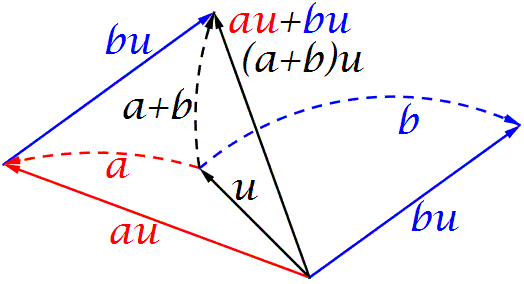
\includegraphics[width=0.5\textwidth]{imagenes/imagenes01/T01IM01.png}
		%\caption{Los dos problemas clásicos del cálculo: trazado de tangentes y áreas bajo curvas.}
	%\end{figure}
		
%varios párrafos encuadrados - explicaciones ad hoc
%\centering{
%\fbox{
%\parbox{0.95\textwidth}{
%varios
%
%$parrafos
%
%dentro
%}
%}
%}
% \justify


%\rotatebox{180}{\leftline{\textcolor{gris}{tararí}}}.
\part{Geometría}



\begin{myexampleblock}{Geometría}
	
\begin{footnotesize}

\vspace{2mm} Etimológicamente hablando, la palabra Geometría procede del griego y significa ``Medida de la Tierra''. La Geometría es la parte de las Matemáticas que estudia las idealizaciones del espacio.

\vspace{2mm} La Geometría no estudia el espacio real en sí mismo, sino objetos ideales (también conocidos como objetos matemáticos o geométricos), sus propiedades, relaciones y teorías, construidos por abstracción de cualidades del espacio real o de otros objetos ideales creados previamente (en el espacio real no existen círculos, pentágonos, rectas, puntos, esferas... sino objetos que tienen forma de... o modelizados por...; la realidad física siempre es menos perfecta que la realidad geométrica pensada o ideal). \textcolor{gris}{\emph{``Las nubes no son esferas, las montañas no son conos, las costas no son círculos y la corteza de los árboles no es lisa, ni los rayos viajan en línea recta'' (Benoit Mandelbrot, `La geometría fractal de la naturaleza', 1980})}

\vspace{2mm} Los componentes elementales de las figuras geométricas serán:

1 Punto: Un punto es un objeto que no tiene dimensiones que indica una posición en el espacio. Se suelen designar con letras mayúsculas A, B, C,... P,…

2 Recta: Es una línea ilimitada por ambos extremos. Se suele denotar con letras minúsculas r, s, t,... Como representación en la realidad de una recta podemos tomar un hilo tenso, o el borde de una regla.
 
3 Plano: es una superficie ilimitada cuya concreción en el mundo real puede verse, por ejemplo, en la superficie de una mesa, una hoja de papel,... Se suele representar con las letras griegas $\pi, \sigma, \tau, \cdots$

\vspace{2mm} Los puntos son objetos de la geometría lineal, puntos y rectas dan lugar a la geometría plana y los puntos, las rectas y los planos son objetos de la geometría espacial.

\vspace{2mm} La geometría analítica es la rama de la geometría en la que las líneas rectas, las curvas y las figuras geométricas se representan mediante expresiones algebraicas y numéricas, cualquier punto del plano se puede localizar por sus tres coordenadas en lo que llamaremos un sistema de regencia.

\vspace{2mm} La fundación de este tipo de geometría se atribuye a René Descartes, quien usó su nombre latinizado, Renatus Cartesius, y por esta razón se conoce con el nombre de ejes cartesianos. Descartes fue un destacado filósofo y matemático francés el y, a mediados del siglo XVII, sentó las bases para el desarrollo de esta disciplina. Se considera uno de los padres del conocimiento científico moderno.

\vspace{2mm} A diferencia de la forma clásica de la geometría (Geometría Euclidiana) que se desprende de un razonamiento lógico-deductivo, la geometría analítica representa de forma gráfica a las figuras geométricas mediante fórmulas matemáticas.



\vspace{2mm} MODERNOS AVANCES.

\vspace{2mm} La geometría sufrió un cambio radical de dirección en el siglo XIX. Los matemáticos Carl Friedrich Gauss, Nikolái Lobachevski, y János Bolyai, trabajando por separado, desarrollaron sistemas coherentes de geometría no euclídea. Estos sistemas aparecieron a partir de los trabajos sobre el llamado "postulado paralelo" de Euclides, al proponer alternativas que generan modelos extraños y no intuitivos de espacio, aunque, eso sí, coherentes.

\vspace{2mm} Casi al mismo tiempo, el matemático británico Arthur Cayley desarrolló la geometría para espacios con más de tres dimensiones. Imaginemos que una línea es un espacio unidimensional. Si cada uno de los puntos de la línea se sustituye por una línea perpendicular a ella, se crea un plano, o espacio bidimensional. De la misma manera, si cada punto del plano se sustituye por una línea perpendicular a él, se genera un espacio tridimensional. Yendo más lejos, si cada punto del espacio tridimensional se sustituye por una línea perpendicular, tendremos un espacio tetradimensional. El uso de conceptos con más de tres dimensiones tiene un importante número de aplicaciones en las ciencias físicas, en particular en el desarrollo de teorías de la relatividad que necesita de cuatro dimensiones.

\vspace{2mm} Otro concepto dimensional, el de dimensiones fraccionarias, apareció en el siglo XIX. En la década de 1970 el concepto se desarrolló como la geometría fractal.


\vspace{2mm} La geometría algebraica es una rama de la matemática que, como sugiere su nombre, combina el álgebra abstracta, especialmente el álgebra conmutativa, con la geometría analítica. Se puede comprender como el estudio de los conjuntos de soluciones de los sistemas de ecuaciones algebraicas. Cuando hay más de una variable, aparecen las consideraciones geométricas que son importantes para entender el fenómeno. Podemos decir que la materia en cuestión comienza cuando abandonamos la mera solución de ecuaciones, y el tema de `entender' todas las soluciones se vuelve tan importante como el de encontrar alguna solución.

\vspace{2mm} 
.

\end{footnotesize}

\end{myexampleblock}






\chapter{Vectores en el espacio}
	


\begin{myblock}{Geometría vs. Álgebra}
	
	\begin{figure}[H]
		\centering
		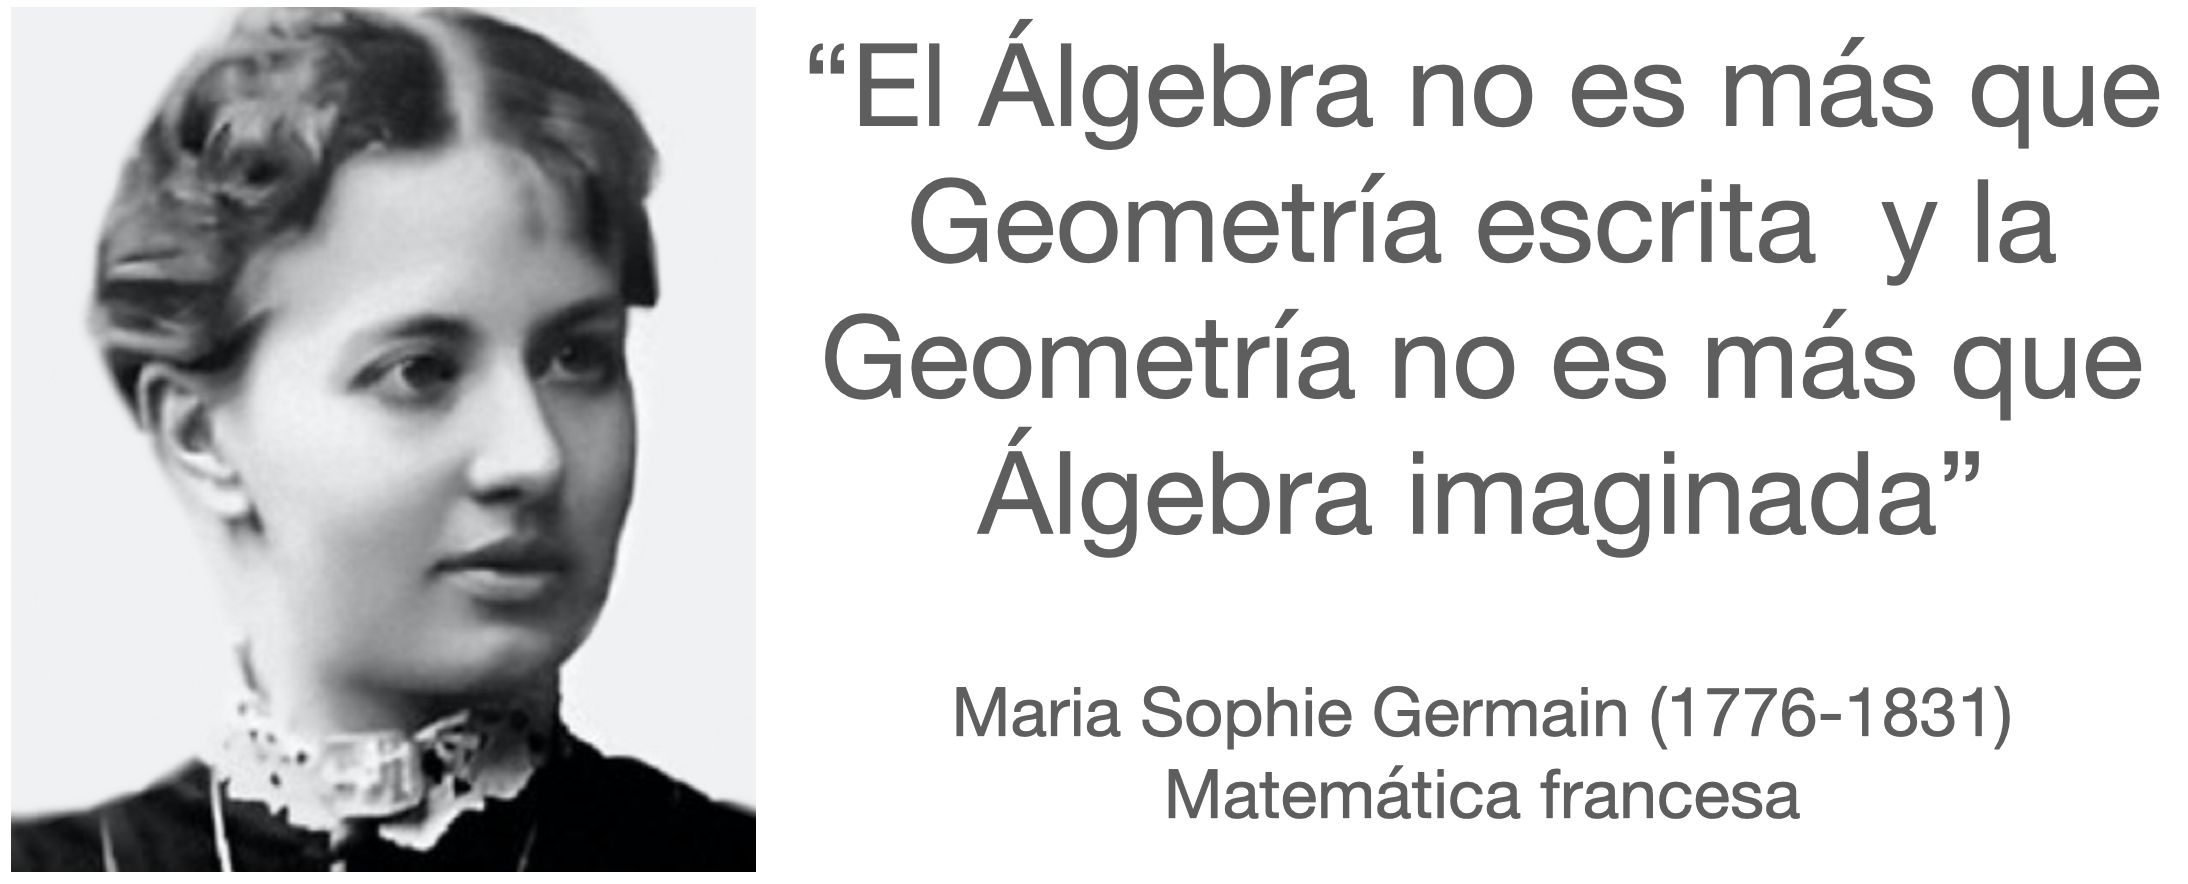
\includegraphics[width=.9\textwidth]{imagenes/imagenes09/Sophie-Germain.png}
	\end{figure}

\end{myblock}



\section[El espacio vectorial de los vectores libres del espacio]{El espacio vectorial de los vectores libres del espacio \sectionmark{E.V. de los Vectores libres}}

\sectionmark{E.V. de los Vectores libres}

$E_3=\{\text{conjunto puntos del espacio}\}=\{A, B, C, \cdots \}$

$V_3=\{\text{conjunto `vectores libres' del espacio}\}=\{\vec u, \vec v, \vec w, \cdots \}$

\normalsize{Las} definiciones que se dan a continuación se muestran en la figura siguiente.

\begin{defi}
Dados dos puntos fijos $A$ y $B$ del espacio de puntos $E_3$, se llama \textbf{`vector fijo'} $\overrightarrow {AB}$ al segmento orientado con origen en $A$ y extremo en $B$.	
\end{defi}

Dos puntos $A$ y $B$ determinan un solo segmento, $\overline{AB}=\overline{BA}$ y dos vectores fijos  $\overrightarrow {AB}$ y  $\overrightarrow {BA}$.

Un vector fijo se dice que es el vector nulo cuando su origen y extremo coinciden: $\boldsymbol{\vec 0}= \overrightarrow {AA} =\overrightarrow {BB} = \overrightarrow {CC}=\cdots$

\vspace{2mm} \begin{defi}{Características de un vector}

Además de extremo y origen, en un vector fijo podemos observar:

--- \textbf{Módulo} de un vector fijo $\overrightarrow {AB}$: es la longitud del segmento $\overrightarrow {AB}$ y se representa por  $|\overrightarrow {AB|}$


--- \textbf{Dirección} de un vector fijo $\overrightarrow {AB}$: es la determinada por la recta que pasa por los puntos $A$ y $B$ y todas las rectas paralelas a ella \textcolor{gris}{(todas las rectas paralelas tienen la misma dirección)}.

Dos vectores fijos  no nulos $\overrightarrow {AB}$ y  $\overrightarrow {CD}$ tienen la misma dirección si y solo si están situados sobre la misma recta o sobre rectas paralelas, se dice  que los vectores son paralelos: $\overrightarrow {AB}\; ||\; \overrightarrow {AB}$


--- \textbf{Sentido} de un vector fijo $\overrightarrow {AB}$: el que va desde el origen $A$ hasta el extremo $B$.

Toda dirección tiene dos sentidos. Em la figura, $\overrightarrow {AB}$ tiene el mismo sentido que $\overrightarrow {GH}$ pero sentido contrario a $\overrightarrow {CD}$: $\quad \overrightarrow {AB} \uparrow\uparrow \overrightarrow {GH}\; $; $\; \overrightarrow {AB} \uparrow \downarrow \overrightarrow {CD}$

\end{defi}

\begin{defi}{Vectores opuestos}

Dos puntos fijos del plano $A$ y $B$ determinan dos vectores $\overrightarrow {AB}$ y $\overrightarrow {BA}$ que se llaman \textbf{`opuestos'}.
	
\end{defi}

\begin{figure}[H]
	\centering
	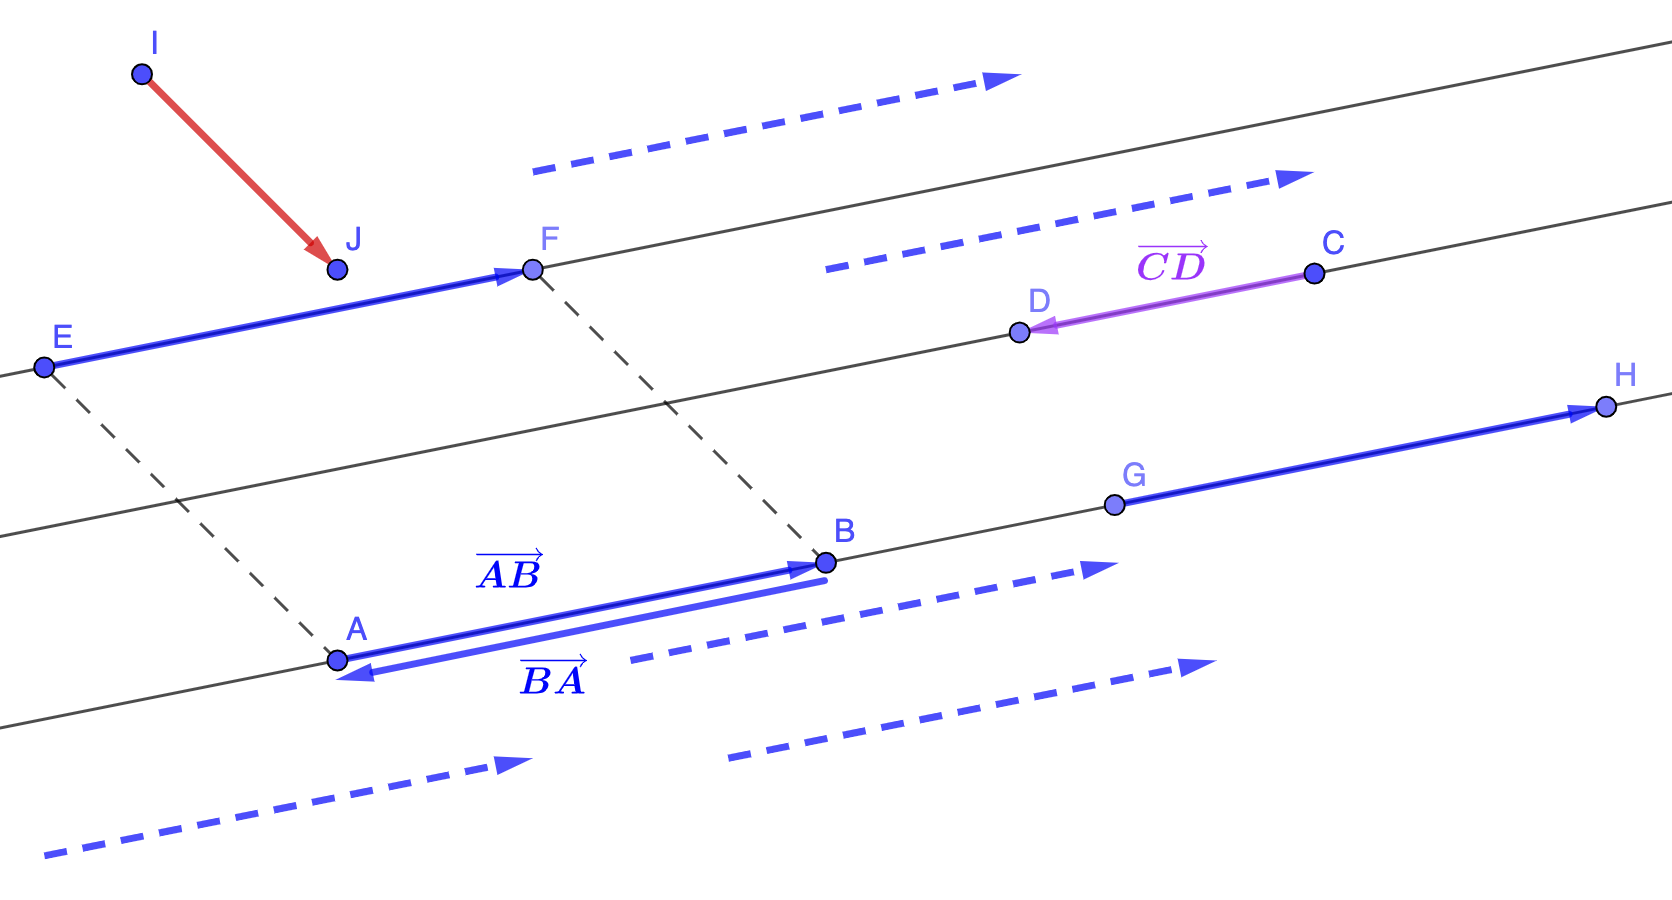
\includegraphics[width=.80\textwidth]{imagenes/imagenes09/T09IM01.png}
\end{figure}



Evidentemente, dos vectores fijos y opuestos tienen el mismo módulo, la misma dirección y sentidos contrarios:

$|\overrightarrow {AB}|=|\overrightarrow {BA}|; \quad \overrightarrow {AB}\; ||\; \overrightarrow {BA}; \quad \overrightarrow {AB} \uparrow\downarrow \overrightarrow {BA}$

\begin{defi}{Vectores equipolentes}

Dados dos vectores fijos $\overrightarrow {AB}$ y $\overrightarrow {GH}$ son `equipolentes' ($\overrightarrow {AB} \boldsymbol{\sim} \overrightarrow {GF}$) si tienen el mismo módulo, la misma dirección y el mismo sentido.
\end{defi}

En la figura anterior so observa que: 

$\overrightarrow {AB} \boldsymbol{\sim} \overrightarrow {GF} \;\; \longleftrightarrow \;\; 
|\overrightarrow {AB}|=|\overrightarrow {GH}| \;\; \wedge \;\; \overrightarrow {AB} \;||\; \overrightarrow {GH} \;\; \wedge \;\; \overrightarrow {AB} \uparrow\uparrow \overrightarrow {GH}$



\begin{prop}
	Si dos vectores fijos no nulos son equipolentes, entonces , o bien están en la misma recta ($\; \overrightarrow {AB} \text{ y } \overrightarrow {GH}\;$), es decir, $A,B,C,D$ están alineados, o bien el cuadrilátero $A,B,C,D$ obtenido al unir los orígenes y los extremos de los vectores se forma el `paralelogramo' $ABEF\; $ ($\; \overrightarrow {AB} \text{ y } \overrightarrow {EF}\;$). Ver figura anterior.
\end{prop}



\begin{defi}{\textbf{Vectores libres}}

Dado un vector fijo $\overrightarrow {AB}$, todos los vectores `equipolentes' a él definen el mismo \textbf{`vector libre'} $\boldsymbol{ \vec u }$ (dibujados en modo discontinuo en la figura anterior). $\vec u=\{\text{vector fijo } \overrightarrow {AB} \text{ y todos sus equipolentes} \}$

Al conjunto de todos los vectores libres del espacio $\mathbb R^3$ le llamamos $V_3$. 

`Módulo, dirección y sentido' de un vector libre es el módulo, dirección y sentido de uno cualquiera de sus vectores equipolentes.	
\end{defi}

Podemos considerar un `vector libre' como una \textit{flecha} que podemos dibujar con origen en cualquier punto con la única condición de no cambiar el tamaño (módulo), la dirección y el sentido.

Los vectores libres van a ser objetos matemáticos (de $V_3$) cuya función va a ser mover puntos (de $E_3$).

\subsection{Operaciones con vectores libres}

\subsubsection{--- Suma de vectores}

\begin{defi}
Dados $\vec u, \vec v \in V_3$, se define el vector suma, $\vec u + \vec v$	,  como aquel que se obtiene:

\begin{multicols}{2}
\begin{itemize}
\item `vectores concurrentes': dibujado el vector $\vec u$, con origen en su extremo dibujamos el vector $\vec v$. Entonces, el vector que va desde el origen de $\vec u$ hasta el extremo de $\vec v$ es el vector suma $\vec u + \vec v$.
\item `método del paralelogramos': dibujamos los vectores $\vec u$ y  $\vec v$  con el origen común (en el mismo punto de $E_3$) y construimos el paralelogramo formado por estos dos vectores (ver figura adjunta). Entonces, el vector suma, $\vec u + \vec v$, es el vector que sale del origen de ambos vectores y llega al extremo opuesto en la diagonal del paralelogramo.	
\end{itemize}

\begin{figure}[H]
	\centering
	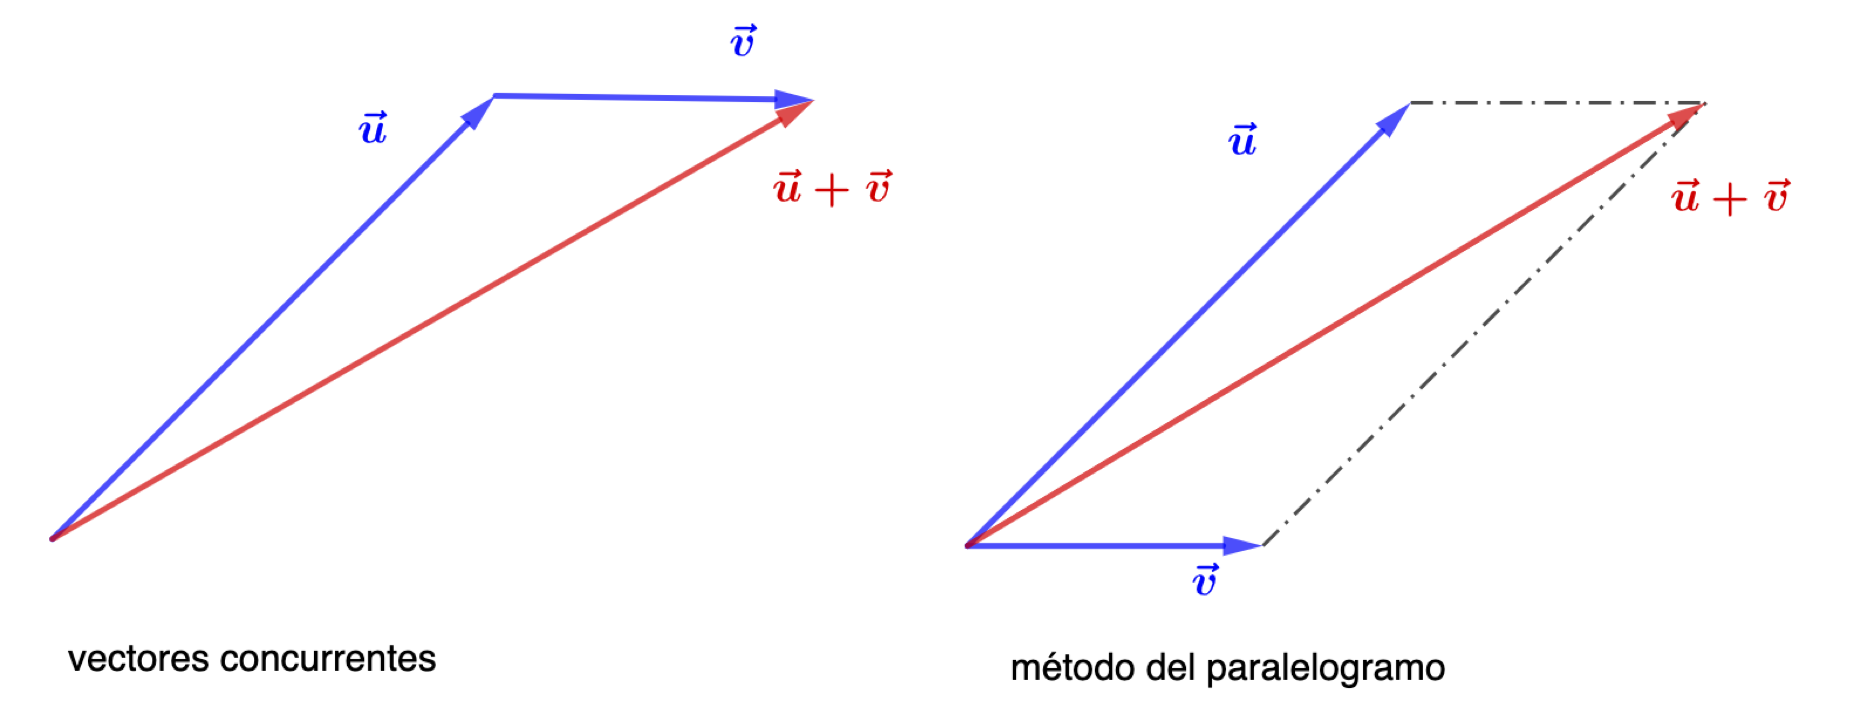
\includegraphics[width=.45\textwidth]{imagenes/imagenes09/T09IM02.png}
	\caption*{Suma de vectores libres}
\end{figure}

\end{multicols}
\end{defi}

\begin{prop}{Propiedades de la suma de vectores libres}

\begin{multicols}{2}
\begin{figure}[H]
	\centering
	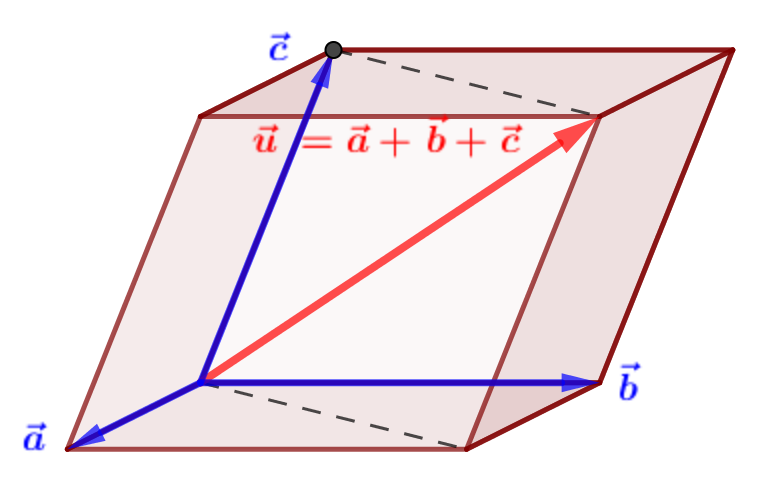
\includegraphics[width=.4\textwidth]{imagenes/imagenes09/T09IM02b.png}
\end{figure}
\begin{itemize}
\item \footnotesize{Conmutativa: $\vec u + \vec v=\vec v + \vec u$}
\item Asociativa: $\vec u + (\vec v+ \vec w)=(\vec u + \vec v)+\vec w$
\item Neutro: $\vec u + \vec 0=\vec 0+\vec u=\vec u$
\item Opuesto: $\vec u+ (\vec{-u})=(\vec{-u})+\vec u= \vec 0$
\end{itemize}
\end{multicols}
	\textcolor{gris}{\normalsize{Con} estas propiedades, $(V_3,+)$ tiene estructura algebraica de grupo abeliano (tema \ref{e_alg} de estructuras algebraicas).}
\end{prop}

\begin{defi}{Diferencia de vectores}
\begin{multicols}{2}
	Llamaremos diferencia (resta) de dos vectores a la suma del primero de ellos con el opuesto del segundo: 
	$\quad \vec u - \vec v = \vec u + (\vec {-v})$
	
\begin{figure}[H]
	\centering
	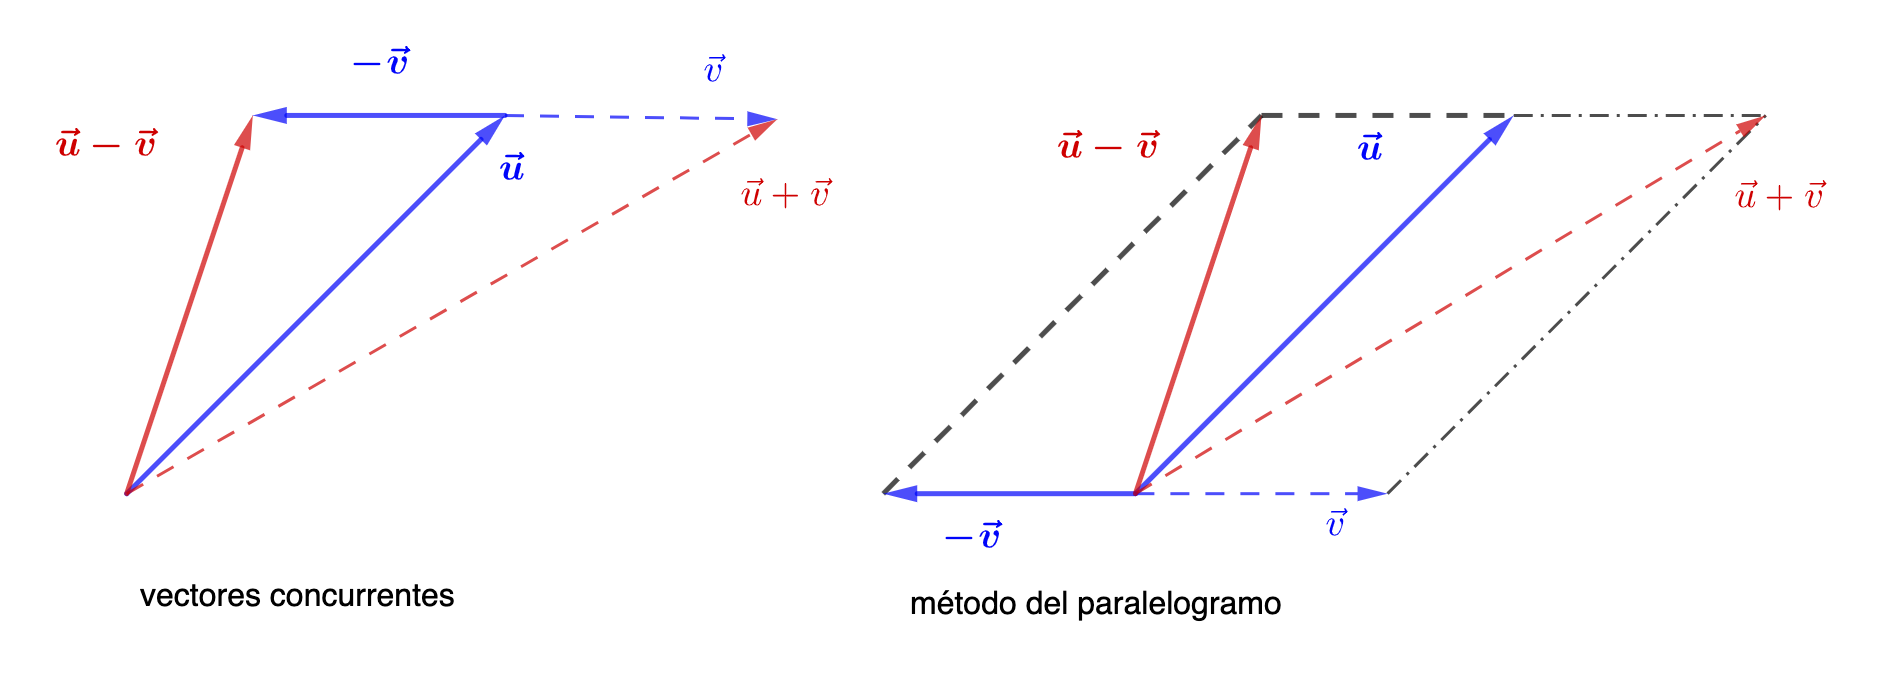
\includegraphics[width=.6\textwidth]{imagenes/imagenes09/T09IM03.png}
	\end{figure}
	
\end{multicols}
\end{defi}

\subsubsection{--- Producto de un vector libre por un escalar}

A los números reales, por contraposición a los vectores, se les llama `escalares'.

\begin{defi}

Sea $k\in \mathbb R; \; \vec u \in V_3$, se define el producto de $k$ por $\vec u$, como aquel vector $k \vec u$ que tiene por:

\tiny{$\blacksquare$} \normalsize{módulo}: $|k\vec u|= abs(k) \cdot mod(\vec u)=|k|\;|\vec u|$
\begin{multicols}{2}
\begin{itemize}
\item direción: la misma que $\vec u$
\item sentido: $\begin{cases} \text{ mismo que } \vec u \text{ si } k>0\\ \text{ contrario a } \vec u \text{ si } k<0	\end{cases} = \begin{cases} \; k\vec u \; \uparrow \uparrow \; \vec u \; \leftrightarrow \; k>0 \\ \; k\vec u \; \uparrow \downarrow \; \vec u \; \leftrightarrow \; k<0 \end{cases}$
\end{itemize}

\begin{figure}[H]
	\centering
	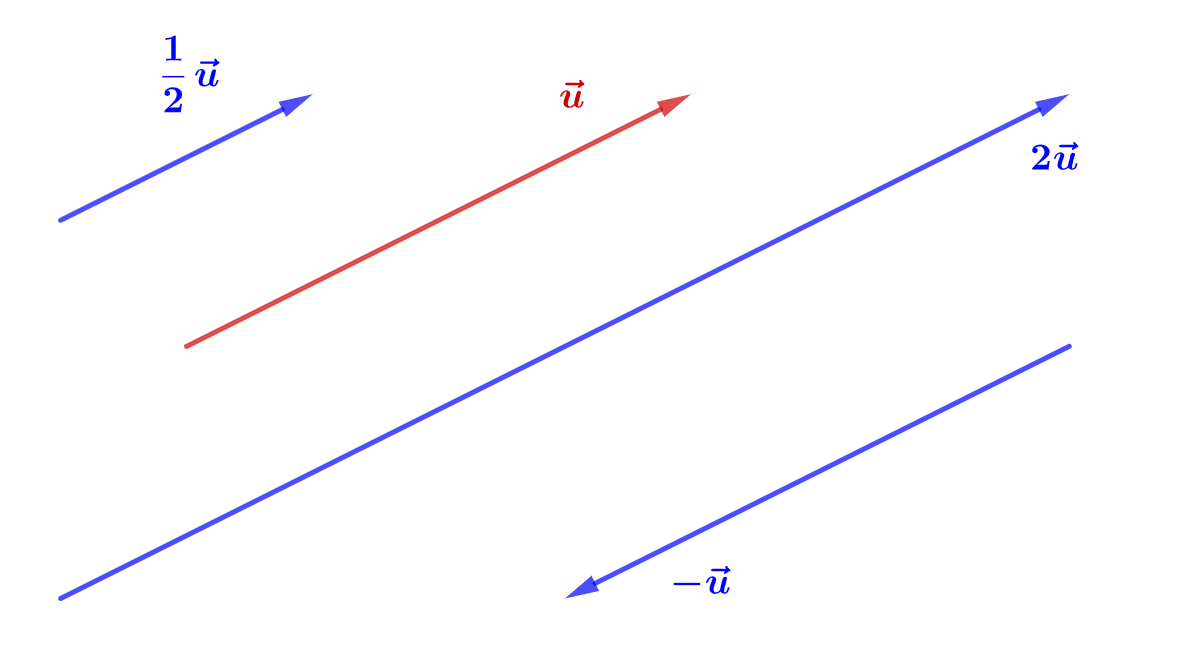
\includegraphics[width=.4\textwidth]{imagenes/imagenes09/T09IM04.png}
	\caption*{Producto por un escalar}
\end{figure}
\end{multicols}
	
\end{defi}

\begin{prop}{Propiedades del producto por un escalar}
\begin{multicols}{2}
\begin{itemize}
\item $k(\vec u + \vec v)=k \vec u + k \vec v$
\item $(k+h)\vec u=k\vec u + h\vec u$	
\item $(kh)\vec u=k(h\vec u)$
\item $1\vec u=\vec u$
\end{itemize}
\end{multicols}	
\textcolor{gris}{\normalsize{Con} estas propiedades, la terna $(V_3,+,\cdot)$ tiene estructura algebraica de espacio vectorial real (tema \ref{e_vec} de espacios vectoriales).}
\end{prop}

\subsection{Sistema de Referencia: coordenadas de un punto, componentes de un vector.}



$3$ vectores $\{ \; \vec u_1,\; \vec u_2, \; \vec u_3 \; \}$ de $V_3$ de distintas direcciones y no coplanarios son LI por lo que forman una \textbf{base} $B_{V_3}$: 

$\; \forall \vec u \in V_3\; \exists ! x \in \mathbb R, \; \exists ! y \in \mathbb R, \; \exists ! z \in \mathbb R\; \therefore \; \vec u=x\vec u_1+y \vec u_2+z \vec u_3$

\begin{defi}.

\begin{multicols}{2}
Llamaremos \textbf{Sistema de Referencia, $\boldsymbol{\mathcal R}$,} al concurso de un punto fijo del espacio de puntos, que llamaremos `origen', $\mathcal O \in E_3$ y una base del espacio vectorial $B=\{ \; \vec u_1,\; \vec u_2, \; \vec u_3 \; \}\subset V_3$, es decir: $\boldsymbol{\mathcal R = \{\; \mathcal O\; ; \;  \{ \; \vec u_1,\; \vec u_2, \; \vec u_3 \; \} \; \}}$

	\begin{figure}[H]
	\centering
	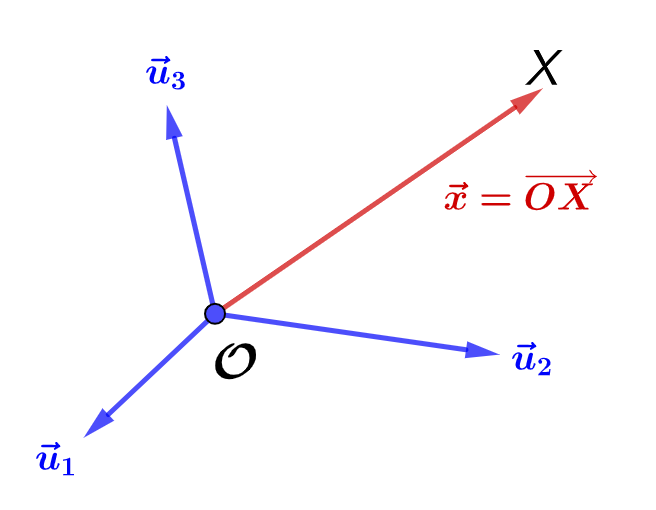
\includegraphics[width=.50\textwidth]{imagenes/imagenes09/T09IM05.png}
	\end{figure}
\end{multicols}

\begin{multicols}{2}
\begin{figure}[H]
	\centering
	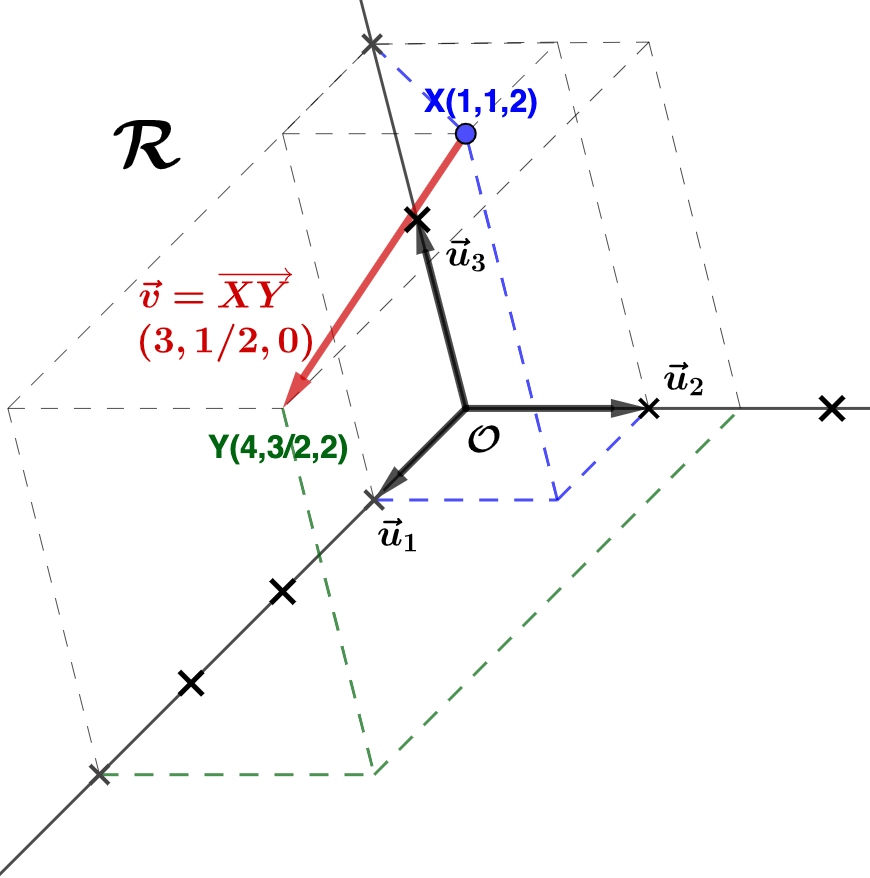
\includegraphics[width=.5\textwidth]{imagenes/imagenes09/T09IM06.png}
	\end{figure}

Para cualquier $X\in E_3$, hay un único vector que desde el origen $\mathcal O$ va hasta $X$, es el `vector de posición' del punto $X$, el vector $\vec x=\overrightarrow{OX}$.

$\vec x$, como vector que es, se escribe de forma única en la base $B$ de $\mathcal R$: $\; \vec x=\alpha \vec u_1 + \beta \vec u_2+ \gamma \vec u_3=(\alpha, \beta, \gamma)$ son las \textbf{componentes} del vector $\vec x$ en $\mathcal R$.
\end{multicols} 

$X$, como punto se puede escribir a través de su vector de posición como $X=(\alpha, \beta, \gamma)$ y ahora hablamos de las \textbf{coordenadas} de $X$ en $\mathcal R$.

\end{defi}


Si dibujamos $\vec v=(v_1,v_2,v_3)$ con origen en $X(x_1,x_2,x_3)$, su extremo será el punto $Y(y_1,y_2,y_3)$ cuyas componentes son $Y(x_1+v_1,x_2+v_2,x_3+v_3)$. De otro modo, llamando $\vec v=\overrightarrow{XY}$ :

$Coord\; Y= Coord\; X + Componentes \; \overrightarrow{XY} \quad $
\colorbox{LightYellow}{$\;\boxed{ \;\boldsymbol{\;Y=X+\overrightarrow{XY}\;\; }} $}

El vector $\vec v=\overrightarrow{XY}$ se desplaza $+3$ veces según el vector $\vec i$ (hacia delante del observador/a), $+1/2$  veces según el vector $\vec j$ (hacia la derecha) y $0$ veces según el vector $\vec k$ (hacia arriba). 

El trabajo de los vectores va a ser desplazar puntos. Al punto $X$ le aplicamos el vector $\vec v=\overrightarrow{XY}$ y lo desplazamos hasta la posición $Y$.



\begin{multicols}{2}
\noindent \textbf{NOTA}: Mientras no se diga lo contrario, las coordenadas del origen será $\mathcal O=(0,0,0)$ y la base que usaremos será la base canónica de $V_3$, formada por los vectores $C_{V_3}=\{\boldsymbol{\vec i}=(1,0,0);\;\boldsymbol{\vec j}=(0,1,0);\;\boldsymbol{\vec k}=(0,0,1)\}$, que forman una base llamada \textbf{`ortonormal'}, sus módulos valen $1$ (`normal'-izado) y son mutuamente perpendiculares (`ortogonales): $\vec i \bot \vec j; \; \vec j \bot \vec k; \; \vec k \bot \vec i$

	\begin{figure}[H]
	\centering
	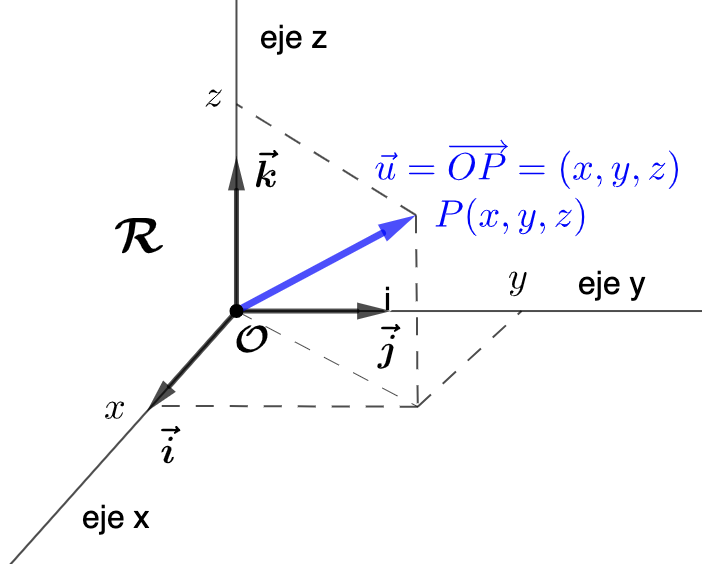
\includegraphics[width=.5\textwidth]{imagenes/imagenes09/T09IM07.png}
	\end{figure}
\end{multicols}

\begin{ejem}

En la siguiente figura, encuentra las coordenadas de los puntos $A,B,C,D,E,F,P$ y del vector $\vec u=\overrightarrow{OP}$	
\end{ejem}

%\clearpage

\begin{multicols}{2}

	\begin{figure}[H]
	\centering
	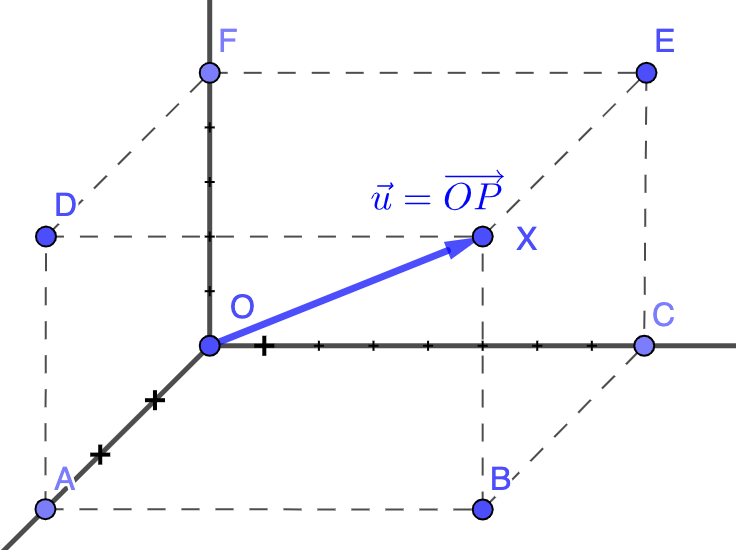
\includegraphics[width=.50\textwidth]{imagenes/imagenes09/T09IM08.png}
	\end{figure}
	
	\textcolor{gris}{$A(3,0,0)\; B(3,8,0); \; C(0,8,0)$}
	
	\textcolor{gris}{$D(3,0,5);\; E(0,8,5); \; F(0,0,5)$}
	
	$\quad$
	
	\textcolor{gris}{$X(3,8,5)$}
	
	\textcolor{gris}{$\vec u=\overrightarrow{OX}=(3,8,5)=3\vec i+8\vec j+5 \vec k$}

\end{multicols}

\subsection{Aplicaciones de los vectores}

\textbf{Componentes del vector que une dos puntos}

\begin{multicols}{2}

	\begin{figure}[H]
	\centering
	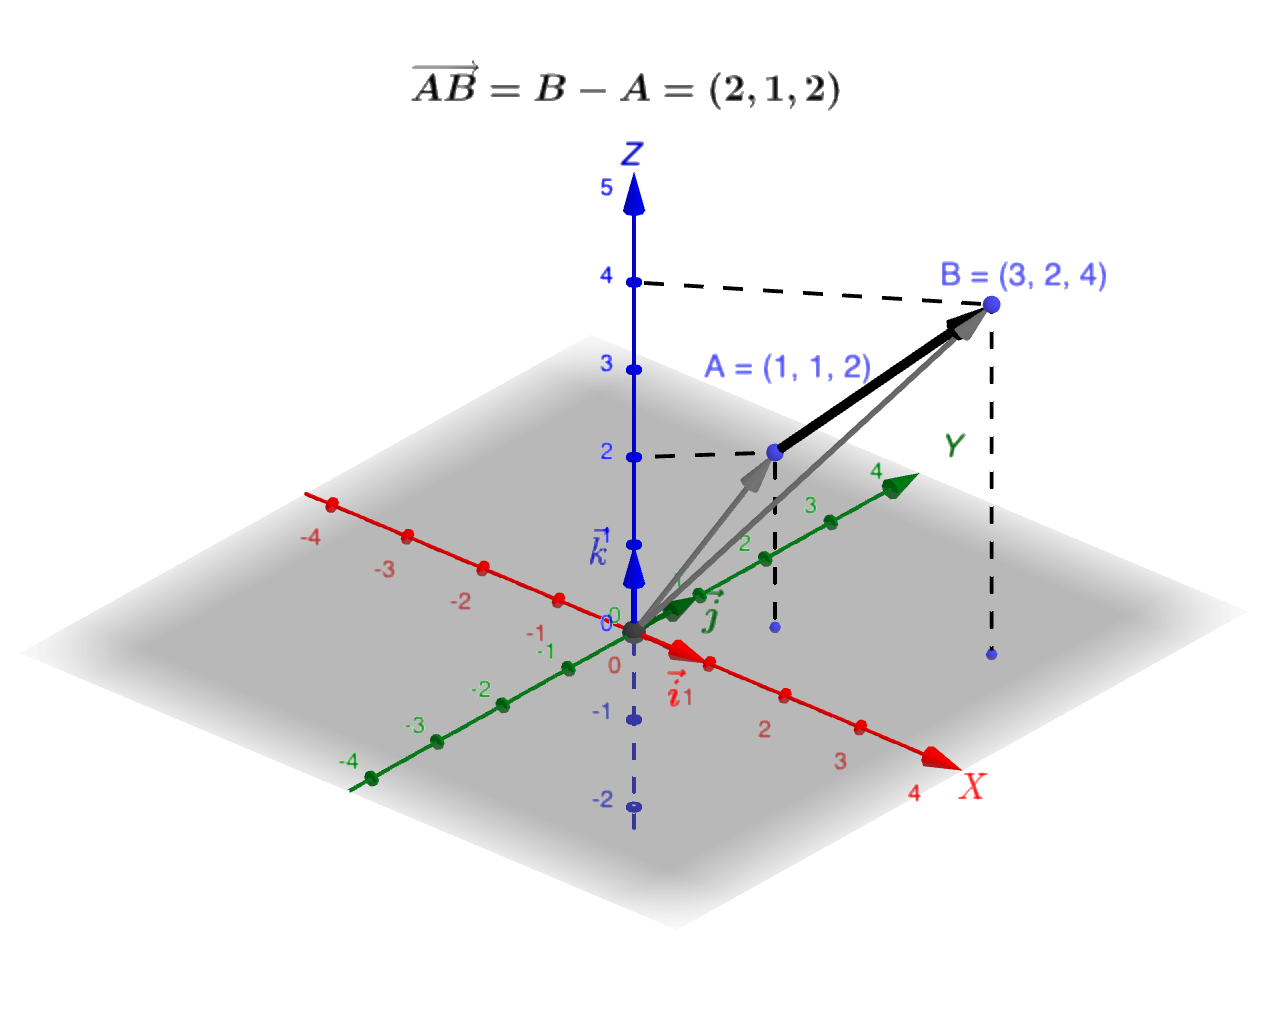
\includegraphics[width=.55\textwidth]{imagenes/imagenes09/T09IM09.png}
	\end{figure}
	
	$\mathcal R\{\mathcal O; \vec i, \vec j, \vec k\}$ sistema de referencia ortonormal, en que $A(a_x,a_y,a_z)$ y $B(b_x,b_y,b_z)$
son las coordenadas de dos puntos. De la figura se observa que:

\noindent $\overrightarrow{OA}+\overrightarrow{AB}=\overrightarrow{OB} \to \overrightarrow{AB}=\overrightarrow{OB}-\overrightarrow{OA}$

\noindent \footnotesize{$A\to \overrightarrow{OA}=(1,1,2); \; B\to \overrightarrow{OA}=(3,2,4)$}

\noindent \normalsize{$\overrightarrow{BA}=B-A=(2,1,2)$}

\end{multicols}



\noindent \small{$\overrightarrow{AB}=\overrightarrow{OB}-\overrightarrow{OA}$}\normalsize{,} abusando del lenguaje podemos decir que: \colorbox{LightYellow}{$\boxed{\; \overrightarrow{AB}=B-A\;}$}, para calcular las componentes, en un sistema de referencia dado, del  vector que representa (une) dos puntos bastará con restar a las coordenadas del punto extremo, las coordenadas del punto origen: \textit{`componentes del vector que une dos puntos = coordenadas del extremo menos coordenadas del origen'.}

Repitiendo lo dicho más arriba, si $\overrightarrow{AB}=B-A$, `despejando' $B=A+\overrightarrow{AB}$  y tenemos, como se ha mencionado anteriormente, que el trabajo de los vectores va a ser desplazar puntos. Al punto $A$ le aplicamos el vector $\overrightarrow{AB}$ y lo desplazamos hasta la posición $B$.

$\mathcal R\{\mathcal O; \vec i, \vec j, \vec k\}$ sistema de referencia ortonormal, las coordenadas del punto $A(a_x,a_y,a_z)$ coinciden con las componentes del vector de posición $\overrightarrow{OA}=a_x\vec i+a_y \vec j+ a_z\vec k=(a_x,a_y,a_z)$, análogamente $B(b_x,b_y,b_z)$ por ser $\overrightarrow{OB}=b_x\vec i + b_y\vec j+b_z\vec k=(b_x,b_y,b_z)$. Las componentes del vector que une los dos puntos, desde $A$ hasta $B$ las obtendremos, abusando del lenguaje, al restar de las coordenadas del extremo $B$ las coordenadas del origen $A$. Decimos abusando del lenguaje porque, evidentemente dos puntos no se pueden restar, lo que hacemos en realidad es definir $\overrightarrow{AB}=\overrightarrow{OB}-\overrightarrow{OB} $ aunque en la  práctica haremos: $\boldsymbol{\overrightarrow{AB}=B-A}$

\vspace{5mm} \textbf{Condición de paralelismo de dos vectores}

De la definición de producto de un vector por un escalar sabemos que el resultado son vectores paralelos, es decir: $\vec u \; || \; \vec v \; \leftrightarrow \; \exists k \in \mathbb R\; / \; \vec u = k\cdot \vec v$

Si $\vec v=(v_x,v_y,v_z) \quad \to \quad k\cdot u=(kv_z,k_vy,kv_z)=(u_x,u_y,u_z) \quad \longrightarrow \quad u_x=kv_x; \;u_y=kv_y; \;u_z=kv_z$, es decir, \textit{\colorbox{LightYellow}{dos vectores son paralelos si sus} \colorbox{LightYellow}{componentes son proporcionales.}} $\quad \dfrac {\vec u_x}{\vec v_x}=\dfrac {\vec u_y}{\vec v_y}=\dfrac {\vec u_z}{\vec v_z}=k$
	
\vspace{3mm} \textbf{Condición de puntos alineados}

\begin{multicols}{2}
Tres puntos $A,\;B$ y $C$ están alineados si, formados dos vectores cualesquiera con ellos tres, éstos resultan paralelos: $\overrightarrow{AB}\;||\;\overrightarrow{AC}$

\begin{figure}[H]
	\centering
	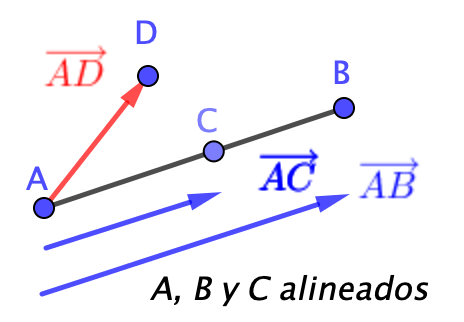
\includegraphics[width=.35\textwidth]{imagenes/imagenes09/T09IM14.png}
\end{figure}
\end{multicols}

\vspace{-5mm} \textbf{Punto medio de un segmento}

\begin{multicols}{2}
Dado el segmento $\overline{AB}$, llamamos ' punto medio' del segmento al punto  $M$ que verifica la ecuación: $\; \overrightarrow{AM}=\frac 1 2 \overrightarrow{AB}\; $

Sean $A(a_x,a_y,a_z); \; B(b_x,b_y,b_z)$ las coordenadas de $A$ y $B$ extremos del segmento, entonces, las coordenadas de $M(m_x,m_y,m_z)$ se pueden escribir como: $m_i=\frac {a_i+b_i}{2},\; \text{ con } i=\{x,y,z\}$

\begin{figure}[H]
	\centering
	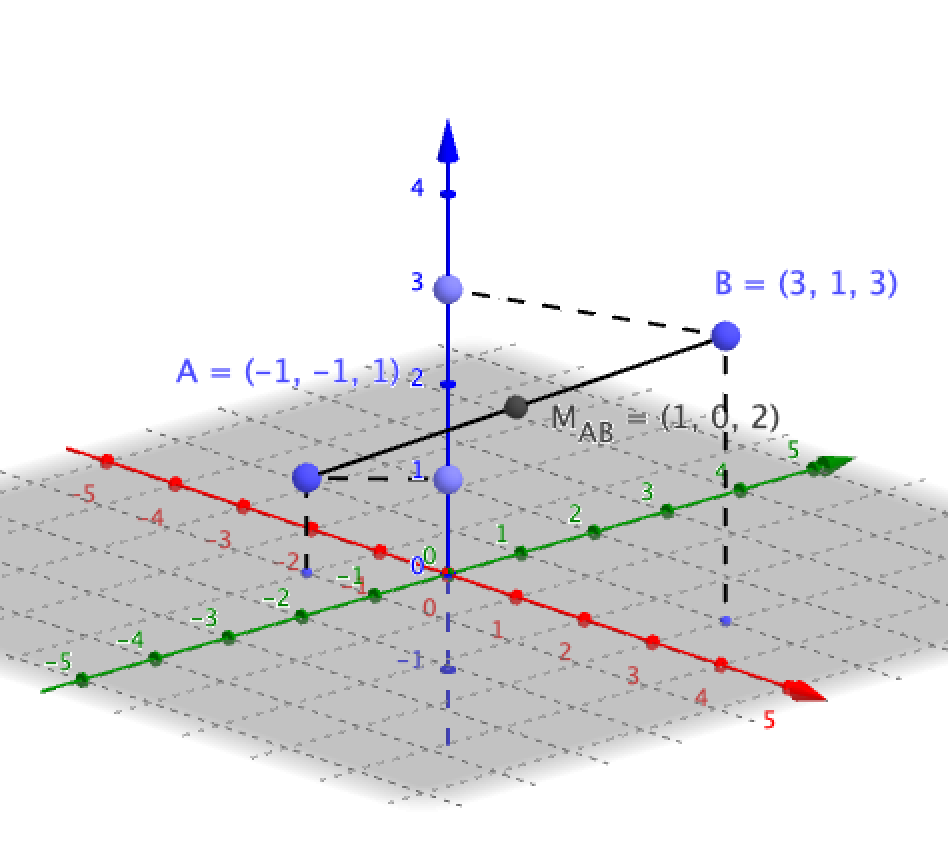
\includegraphics[width=.55\textwidth]{imagenes/imagenes09/T09IM10.png}
\end{figure}
\end{multicols}

\noindent \footnotesize{\textcolor{gris}{$\overrightarrow{AM}=\frac 1 2 \overrightarrow{AB} \to (m_x,m_y,m_z)-(a_x,a_y,a_z)=\frac 1 2 [\;(b_x,b_y,b_z)-(a_x,a_y,a_z)\;]$, despejando, $m_i=\frac {a_i+b_i}{2},\; \text{ con } i=\{x,y,z\}$}}\normalsize{.}

\textit{Las `coordenadas del punto medio' de un segmento las obtendremos como `semisuma de las coordenadas de los extremos'}: \colorbox{LightYellow}{$\; \boxed{\; M_{AB}=\dfrac {A+B}{2}\; }\; $}

\vspace{5mm}\textbf{Simétrico de un punto $\boldsymbol{P}$ respecto de otro  $\boldsymbol{Q}$}
\begin{multicols}{2}
\begin{figure}[H]
	\centering
	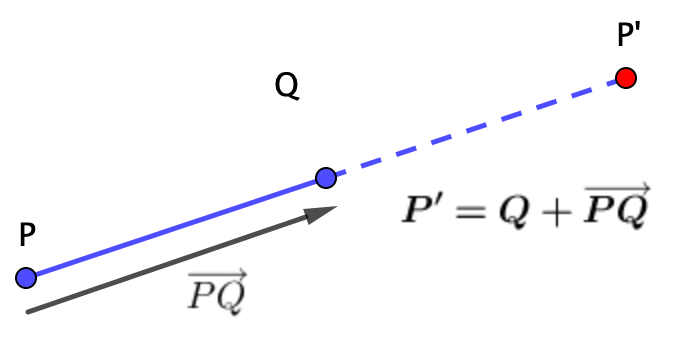
\includegraphics[width=.45\textwidth]{imagenes/imagenes09/T09IM12.png}
\end{figure}
Dados $P$ y $Q$, el simétrico de $P$ respecto de $Q$ ha de ser un punto $P'$ tal que $Q$ sea el punto medio del segmento $\overline{PP'}$.


\end{multicols}
Es decir, $P'=Q+\overrightarrow{PQ}$, en coordenadas: \colorbox{LightYellow}{$\boxed{\;\dfrac {P+P'}{2}=Q \to P'=2Q-P\;}$} \textcolor{gris}{(abusando del lenguaje)}

\vspace{5mm} \textbf{División de un segmento en $\boldsymbol{ n }$ partes.}

\begin{multicols}{2}

Dados los puntos $A$ y $B$, formamos el vector $\overrightarrow{AB}$ y, a partir de él, $\frac 1 n \overrightarrow{AB}$. Si a $A$ le sumamos este último vector llegamos al punto $A_1=A+\frac 1 n \overrightarrow{AB}$; análogamente, $A_2=A+\frac 2 n \overrightarrow{AB}$ y, en general, 
\begin{figure}[H]
	\centering
	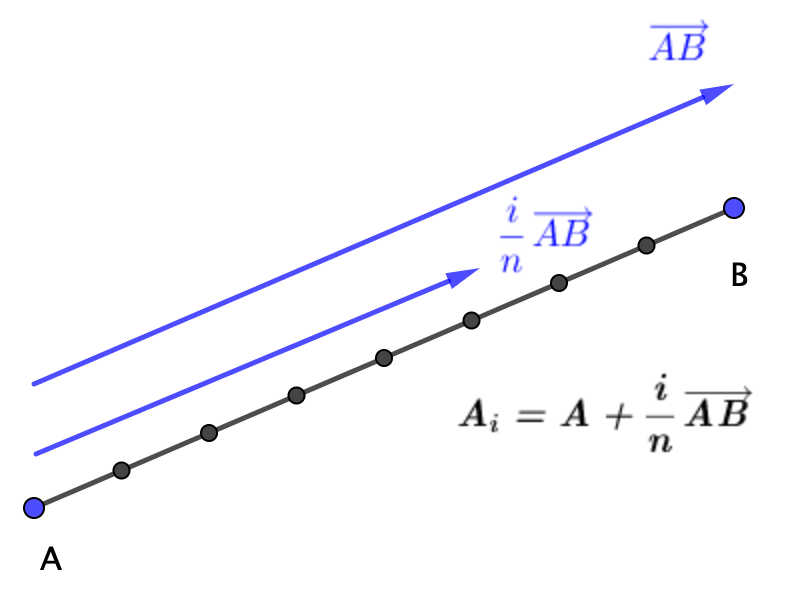
\includegraphics[width=.45\textwidth]{imagenes/imagenes09/T09IM11.png}
\end{figure}

\end{multicols}
\colorbox{LightYellow}{$\boxed{\;A_i=A+\frac i n\;  \overrightarrow{AB}\;}$}. $\quad$ Evidentemente, $A_0=A; \; A_n=B$

\newpage %*****************************************************
\textbf{Baricentro de un triángulo}

\begin{multicols}{2}
\begin{figure}[H]
	\centering
	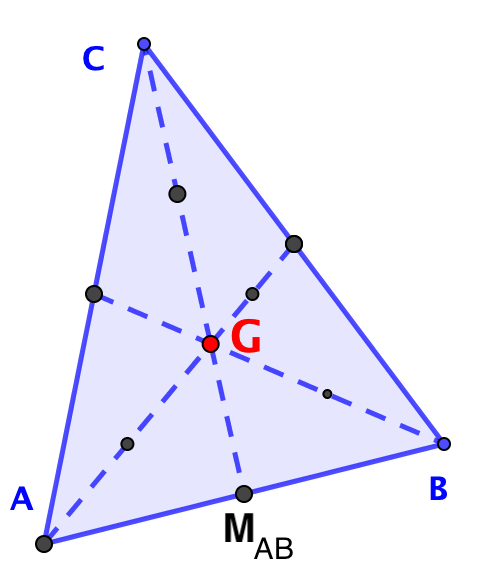
\includegraphics[width=.35\textwidth]{imagenes/imagenes09/T09IM13.png}
\end{figure}

$3$ puntos no alineados $A,B, C$ definen un triángulo. Se llama `baricentro' o `centro de gravedad' de un triángulo, $G$,  al corte de sus medianas \textcolor{gris}{(mediana: recta que va de un vértice de un triángulo al punto medio del lado opuesto; el baricentro dista del vértice el doble que del punto medio)} 

\end{multicols}

De nuevo abusando del lenguaje, se tiene que: \colorbox{LightYellow}{$\boxed{\;G=\frac{A+B+C}{3}\;}\; .$\; }
El baricentro, $G$,  de un triángulo está en la `tercisuma' de sus vértices:



\vspace{3mm}En lo sucesivo usaremos la siguiente \underline{notación}: $\boldsymbol{ P(x,y,z)}$, para los \textbf{puntos} usaremos letras mayúsculas y escribiremos sus componentes sin el símbolo igual, $\boldsymbol{\vec u=(u_x,u_y,u_z)}$, para los  \textbf{vectores} usaremos letras minúsculas, con flechita arriba, y sus componentes las escribiremos después del signo igual.

\begin{ejem}
\small{Considera} los puntos $A(1,2,-3),$ $\; B(4,5,0),$ $\; C(-2,5,3)$ y $D(3,x,-1)$. Se pide:
\begin{enumerate}[a) ]	
\item $\overrightarrow {AB}$ y  $\overrightarrow {BA}$
\item Comprueba que $\overrightarrow {AB}+\overrightarrow {BC}=\overrightarrow{AC}$ 
\textcolor{gris}{(Ley de Chasles)} y que 
$\overrightarrow {AB}+\overrightarrow {BC}+\overrightarrow {CA}=\overrightarrow {0}$
\item Determina el valor de $x$ en $D$ para que $A,B$ y $D$ estén alineados.
\item Idem para  $\overrightarrow {AB}\;||\;\overrightarrow {CD}$	
\item Encuentra el punto medio del segmento  $\overline {AB}$
\item Encuentra las coordenadas de un punto $P$ del segmento  $\overline {AB}$ tal que la distancia a $B$ sea doble que la distancia a $A$
\item Encuentra el baricentro del triángulo de vértices $A,B,C$
\item Comprueba que la distancia del baricentro a un vértice del triángulo es doble que la de éste al punto medio del lado opuesto al vértice.
\end{enumerate}
%\normalsize{---------------------------}

\small{\noindent --- a) $\overrightarrow {AB}=B-A=(3,3,3);\quad \overrightarrow {BA}=A-B=(-3,-3,-3)$, evidentemente, $\overrightarrow {BA}=-\overrightarrow {AB}$}

\noindent --- b) $\overrightarrow {AB}=(3,3,3); \; \overrightarrow {BC}=C-B=(-6,0,3); \; \overrightarrow {AB}+\overrightarrow {BC}=(3,3,3)+(-6,0,3)=(-3,3,6)$

\noindent Por otro lado: $\overrightarrow {AC}=C-A=(-3, 3, 6)$. 

\noindent Luego sí se cumple que $\overrightarrow {AB}+\overrightarrow {BC}=\overrightarrow{AC}$

\noindent --- c) $A,B$ y $D$ están alineados si $\overrightarrow {AB}\;||\;\overrightarrow {AD}$:

\noindent $\overrightarrow {AB}=(3,3,3); \; \overrightarrow {AD}=D-A=(2,x-2,2) \to \frac 2 3 = \frac {x-2} 3 = \frac 2 3 \to x=4$

\noindent --- d) $\overrightarrow {AB}\; ||\; \overrightarrow {CD}$ si sus componentes son proporcionales:

\noindent $\overrightarrow {AB}=(3,3,3); \; \overrightarrow {CD}=D-C=(5, x-5, -4) \to \frac 5 3 = \frac {x-5} 3 =\frac {-4} 3$, evidentemente, $\frac 5 3 \neq \frac {-4} 3 \Rightarrow \nexists \; x\; / \; \overrightarrow {AB}\;|| \; \overrightarrow {CD}$ 

\noindent --- e) $M_{AB}=\dfrac {A+B} 2 = \dfrac {(5,7,-3)}2=(5/2, 7/2, -3/2)$

\noindent --- f) De la figura: 
\begin{multicols}{2}
\noindent$P=A+\frac 2 3 \overrightarrow {AB}$

\noindent$P=(1,2,-3)+\frac 2 3 (3,3,3)$

\noindent$P=(1,2,-3)+(1,1,1)=(2,3,2)$
\begin{figure}[H]
	\centering
	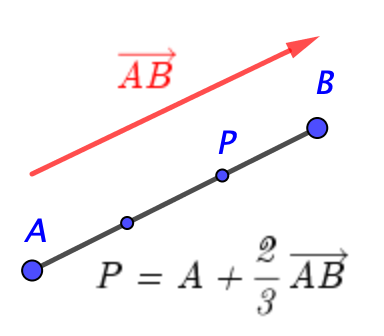
\includegraphics[width=.3\textwidth]{imagenes/imagenes09/T09IM15.png}
\end{figure}
\end{multicols}

\vspace{-8mm}
\noindent --- g) $G=\dfrac {A+B+C} 3 =\dfrac {(3,14,0)} 3 = (1,4,0)$

\noindent --- h) Fijándonos en la figura del apartado `baricentro', se observa que: $G=M_{AB}+\frac 1 3 \overrightarrow{M_{AB}C} \; (*)$

\noindent $M_{AB}=(5/2,7/2,-3/2); \; \overrightarrow{M_{AB}C}=C-M_{AB}=(-2,5,3)-(5/2,7/2,-3/2)=(-9/2,3/2,9/2)$

\noindent $(*)\to G=(5/2,7/2,-3/2)+\frac 1 3 (-9/2,3/2,9/2)=(5/2,7/2,-3/2)+(-3/2,1/2,3/2)=(1,4,0)$, obviamente, el mismo resultado anterior $\qquad \qquad \qquad \qquad \Box\qquad $ \normalsize{.}

\end{ejem}

Vamos ahora a estudiar tres diferentes productos con vectores, el producto escalar, el producto vectorial y el producto mixto, todos ellos con importantes aplicaciones geométricas.
\section{Producto escalar}\label{prodesc}

\begin{defi}
Dados $\vec u, \vec v \in V_3$, se define el producto escalar de dos vectores como el número real (escalar): \colorbox{LightYellow}{$\boxed{\; \vec u \cdot \vec v=|\vec u|\;|\vec v|\; \cos \theta\; }$}$\; \in \mathbb R$, siendo $\theta$ el ángulo que forman $\vec u \text{ y } \vec v$	
\end{defi}

\begin{multicols}{2}
\noindent Interpretación geométrica del producto escalar:

\noindent $\vec u \cdot \vec v=|\vec u|\;|\vec v|\; \cos \theta=|\vec u|\; Proy_{\;\vec u}\;(\vec v)$; 

\noindent siendo $Proy_{\; \vec u}\;(\vec v)=|\vec v|\; \cos \theta$

\begin{figure}[H]
	\centering
	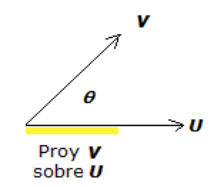
\includegraphics[width=.3\textwidth]{imagenes/imagenes09/T09IM16.png}
\end{figure}
\end{multicols}

\vspace{-5mm} El producto escalar de dos vectores es el módulo de uno de ellos por la proyección del otro sobre él.

\begin{prop}{Propiedad fundamental del producto escalar}

\vspace{3mm} \centerline{\colorbox{LightYellow}{$\; \vec u \; \bot \; \vec v \;  \longleftrightarrow \; \vec u \cdot \vec v = 0\; $}}	
\end{prop}
\justify
\vspace{-3mm} \begin{proofw}
$\boxed{\rightarrow} \quad$	Si $\vec u \; \bot \; \vec v  \longrightarrow \theta=90^o \longrightarrow \vec u \cdot \vec v=|\vec u|\;|\vec v|\; \cancelto{0}{cos (90^o)}=0$

\noindent $\boxed{\leftarrow} \quad$	 Si $\vec u \cdot \vec v = 0$  \scriptsize{y $\vec u\neq \vec 0\; \wedge \; \vec v \neq 0$}  \normalsize{$\to$}  $|\vec u|\;|\vec v|\; \cos \theta=0 \to \cos \theta=0 \longrightarrow $

\noindent $\theta =90^o:\; \vec u \; \bot \; \vec v$
\end{proofw}

\noindent \textbf{Propiedades del producto escalar:}

\noindent $\vec u \cdot \vec v=\vec v \cdot \vec u; \quad \alpha (\vec u \cdot \vec v)=(\alpha \vec u) \cdot \vec v= \vec u \cdot (\alpha \vec v); \quad  \vec u \cdot (\vec v\ + \vec w)= \vec u \cdot \vec v+ \vec u \cdot \vec w$


\noindent \textbf{Aplicaciones del producto escalar:}

\textbf{Módulo de un vector:}

$\vec u \cdot \vec u=|\vec u|\; |\vec u|\; \cancelto{1}{\cos\; 90^o}=|\vec u|^2 \quad \longrightarrow \qquad  \boldsymbol{ |\vec u|=+\sqrt{\vec u \cdot \vec u} }$

\textbf{Ángulo de dos vectores}

$\vec u \cdot \vec v=|\vec u|\;|\vec v|\; \cos \theta \quad \longrightarrow \qquad \boldsymbol{ \cos \theta = \dfrac {\vec u \cdot \vec v}{|\vec u|\; |\vec v|} }$

\textit{Es por esto por lo que muchos autores hablan del producto escalar como la `métrica' del espacio, pues nos permite medir distancias (módulos) y ángulos. Podríamos decir que el producto escalar es la cinta métrica y el goniómetro (transportador) del matemático.}

\begin{multicols}{2}
Aunque parezca existir una cierta ambigüedad a la hora de definir el ángulo que forman dos vectores, pues dado $\cos \theta$ igual a un determinado valor existen dos ángulos posibles $\theta$ y $360^o-\theta$ que lo verifican, la ambigüedad desaparece al definir el ángulo entre dos vectores como el menor de los dos posibles (menor de $180^o$).
\begin{figure}[H]
	\centering
	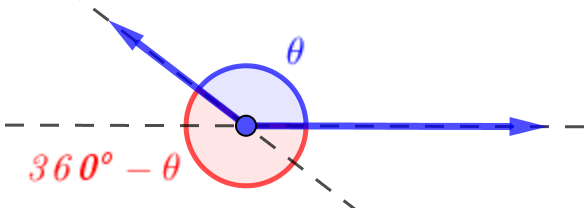
\includegraphics[width=.45\textwidth]{imagenes/imagenes09/T09IM17.png}
\end{figure}
\end{multicols}

\subsection{Expresión del producto escalar en una BON (base ortonormal)}

\begin{prop}
Sea $B=\{ \;  \vec i;\; \vec j;\; \vec k\; \; \therefore \;  \; |\vec i|=|\vec j|=|\vec k|=1 \; \text {  y  } \; \vec i \bot \vec j; \; \vec j \bot \vec k; \; \vec k \bot \vec i \; \}$, una BON y $\vec u,\; \vec v$ dos vectores de $V_3$ cuyas componentes en la BON son:  $\vec u=u_x\vec i+u_y\vec j+u_z\vec k=(u_x,u_y,u_z);\; \; \vec v=v_x\vec i+v_y\vec j+v_z\vec k=(v_x,v_y,v_z)$, se demuestra que:

$\boldsymbol{\vec u \cdot \vec v = u_xv_x+u_yv_y+u_zv_z} \quad \in \mathbb R$

$\boldsymbol{|\vec u|}= + \sqrt{\vec u \cdot \vec u}=\boldsymbol{+\sqrt{u_x^2+u_y^2+u_z^2}}$

$\boldsymbol{\cos \theta} = \dfrac {\vec u \cdot \vec v}{|\vec u|\; |\vec v|}= \boldsymbol{\dfrac {u_xv_x+u_yv_y+u_zv_z }{\sqrt{u_x^2+u_y^2+u_z^2}\; \sqrt{v_x^2+v_y^2+v_z^2}}}$
\end{prop}
\begin{proofw}
Como estamos en una BON, 

\noindent $\vec u \cdot \vec v =(u_x,u_y,u_z)\;(v_x,v_y,v_z)= (u_x\vec i+u_y\vec j+u_z\vec k)\; (v_x\vec i+v_y\vec j+v_z\vec k)= u_x\; u_x \; \cancelto{1}{\cos 0^o+} u_x\; u_y\; \cancelto{0}{\cos 90^o} + \cdots=u_x^2+\cdots $ 

\noindent Teniendo en cuenta lo anterior, es muy sencillo acabar la demostración (hágase).
	
\end{proofw}

\subsection{Normalización de un vector}

\begin{defi}
	Dado un vector $\vec u$, `normalizar' el vector es conseguir otro de la misma dirección y módulo unidad: $\widehat{u}=\; \pm \frac 1 {|\vec u|}\; \vec u$, también se le llama `vector unitario'.. Ambos vectores tienen la misma dirección que $\vec u$, uno con el mismo sentido y otro con sentido contrario.
\end{defi}

Consideremos el vector unitario $\widehat u$, de componentes $\widehat u=(\hat u_x,\hat u_y.\hat u_z)$, como $\widehat u \cdot \vec i=\cancelto{1}{|\widehat u|}\cancelto{1}{|\vec i|}\cos \alpha=\boldsymbol{ \cos \alpha}=(\hat u_x,\hat u_y.\hat u_z)\cdot(1,0,0)=\boldsymbol{\hat u_x}$, siendo $\alpha$ el ángulo que forma $\vec u$ o $\widehat u$ con el eje $OX$ y del mismo modo para los ejes $OY,\; \beta$ y $OZ,\; \gamma$, tenemos que cualquier vector unitario, $\widehat u$, se puede escribir:

\vspace{-3mm}\begin{multicols}{2}
$\widehat u=\cos \alpha \vec i + \cos \beta \vec j + \cos \gamma \vec k=(\cos \alpha, \cos \beta, \cos \gamma)$, que se llaman `cosenos directores' de $\widehat u$. Es decir, las componentes de un vector unitario o normalizado son los cosenos directores del mismo, los cosenos de los ángulos que forma el vector con los ejes coordenados.

\textcolor{gris}{Como $|\widehat u|^2=1 \to $}

\textcolor{gris}{$\cos^2 \alpha + \cos^2 \beta + \cos^2 \gamma=1$}

\begin{figure}[H]
	\centering
	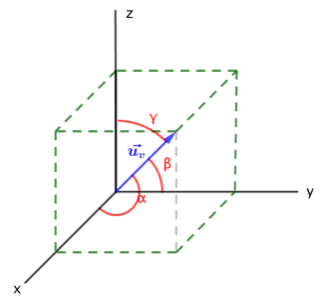
\includegraphics[width=.45\textwidth]{imagenes/imagenes09/T09IM18.png}
\end{figure}
\end{multicols}

\subsection{Distancia entre dos puntos}

\begin{defi}
Dados $A,B \in E_3$ dos puntos del espacio, se define la distancia entre ellos como: $\quad$ \colorbox{LightYellow}{$\; d(A,B)=|\overrightarrow{AB}|\;$}

\noindent \textit{Propiedades}:
$\quad d(A,B)=d(B,A)\; ;  \qquad  d(A,B)=0 \leftrightarrow A=B$.	
\end{defi}

\begin{ejem}
 
\begin{multicols}{2}

Clasifica el triángulo de vértices:
 
$A(3,4,0);\; B(3,0,1); \; C(0,-5,2)$

\begin{figure}[H]
	\centering
	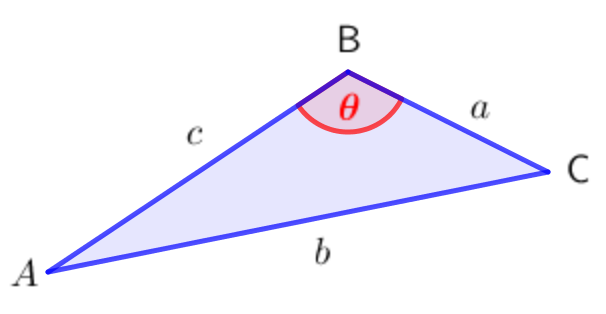
\includegraphics[width=.35\textwidth]{imagenes/imagenes09/T09IM19.png}
\end{figure}
\end{multicols}

$\overrightarrow{AB}=B-A=\;\;(0,-4,1) \to |\overrightarrow{AB}|=\sqrt{0^2+(-4)^2+1^2}=\sqrt{17}\; u=c$

$\overrightarrow{AC}=C-A=(-3,-9,2) \to |\overrightarrow{AB}|=\sqrt{94}\; u=b$

$\overrightarrow{BC}=C-B=(-3,-5,1) \to |\overrightarrow{AB}|=\sqrt{35}\; u=a$

Al ser los tres lados distintos, el triángulo es `escaleno'.

Test de Pitágoras: $\sqrt{94}^2 > \sqrt{35}^2+\sqrt{17}^2 \to$ el triángulo es `obtusángulo' en $B$.

Cálculo del ángulo $B$: $\overrightarrow{BC}=(-3,-5,1)\; \quad \overrightarrow{BA}=-\overrightarrow{AB}=(0,4,-1)$

$\overrightarrow{BC}\cdot \overrightarrow{BA}=(-3,-5,1)\cdot (0,4,-1)=0-20-1=-21$

$|\overrightarrow{BC}|\;|\overrightarrow{BA}|\cos B=\sqrt{35} \sqrt{17} \cos \theta$

Luego, $-21=\sqrt{35} \sqrt{17} \cos \theta \longrightarrow \theta = 149.42^o$. Por lo que el área del triángulo será: $S=\frac 1 2 a c \sin B=\frac 1 2 \sqrt{35} \sqrt{17} \sin 149.42^o= 6.20 u^2$
\end{ejem}

\section{Producto vectorial}

\begin{defi}
El producto vectorial de dos vectores $\vec u$ y $\vec v$ es un nuevo vector $\vec u \times \vec v$	 tal que:

	\begin{multicols}{2}				
	--- su módulo es $|\vec u \times \vec v|=|\vec u||\vec v| \sin \theta $, \small{con $\theta$ el ángulo que forman $\vec u$ y $\vec v$}\normalsize{.}
				
	---  su dirección es perpendicular al plano que forman $\vec u$ y $\vec v$.
				
	---  y su sentido es el de avance del giro de un sacacorchos que intente llevar el vector $\vec u$ hacia el $\vec v$ por el camino más corto.
	
	\begin{figure}[H]
	\centering
	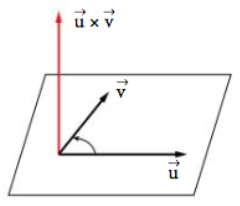
\includegraphics[width=.45\textwidth]{imagenes/imagenes09/T09IM20.png}
	\end{figure}
	\end{multicols}

\end{defi}


\textbf{Propiedades del producto vectorial}

\begin{multicols}{2}


\noindent $\bullet $ El \underline{módulo} del producto vectorial mide el \underline{área del paralelogramo} que forman los vectores $\vec u$ y $\vec v$:

$ |\vec u \times \vec v|=|\vec u||\vec v| \sin \theta$
\begin{figure}[H]
	\centering
	\includegraphics[width=.3\textwidth]{imagenes/imagenes09/T09IM21.png}
	\end{figure}
	\end{multicols}


\begin{itemize}
\item ¡El producto vectorial es \underline{no-conmutativo}!: $\vec u \times \vec v=-\vec v \times \vec u$

		
\vspace{-2mm} \item  $\vec u \times \vec u=\vec 0$
		
\vspace{-2mm} \item  Tomaremos la BON \underline{orientada}, $\vec i \times \vec j = \vec k$; $\vec j \times \vec k = \vec i$ y $\vec k \times \vec i = \vec j$
		
\vspace{-2mm} \item  $(\alpha \vec u)\times \vec v=\alpha (\vec u \times \vec v)= \vec u \times (\alpha \vec v)$
		
\vspace{-2mm} \item  ¡\underline{No} se cumple la \underline{asociativa}!: $\vec u \times (\vec v \times \vec w) \neq (\vec u \times \vec v)\times \vec w$
		
\vspace{-2mm} \item  \underline{Distributivas}: $\vec u \times (\vec v + \vec w)= \vec u \times \vec v + \vec u \times \vec w$; $(\vec u + \vec v)\times \vec w=\vec u \times \vec w + \vec v \times \vec w$
		
\vspace{-2mm} \item  En componentes, el desarrollo del producto vectorial es un determinante:
		
\centerline{\colorbox{LightYellow}{$\; \boldsymbol {\overrightarrow { u } \times \overrightarrow { v } \quad =\quad \left| \begin{matrix} \overrightarrow { i }  & \overrightarrow { j }  & \overrightarrow { k }  \\ u_x & u_y & u_z \\ v_x & v_y & v_z \end{matrix} \right|}\;  $}}

\vspace{-2mm} \item $\vec u \times \vec v$ siempre es un vector perpendicular a $\vec u$ y a $\vec v$ y su módulo representa el área del paralelogramos que definen estos dos vectores.
\end{itemize}
\justify

\begin{figure}[H]
	\centering
	\includegraphics[width=.9\textwidth]{imagenes/imagenes09/T09IM22.png}
	\caption*{Afortunadamente, el producto vectorial no es asociativo.}
	\end{figure}
	
\begin{ejem}
Los tres puntos siguientes forman un triángulo, calcula su área usando el producto vectorial.  $\quad A(3,4,0);\; B(3,0,1); \; C(0,-5,2)$	
\end{ejem}
\begin{multicols}{2}
Consideremos los vectores $\overrightarrow{AB}$ y $\overrightarrow{AC}$, entonces, el módulo del vector producto vectorial de ambos, $|\overrightarrow{AB} \times \overrightarrow{AC}|$, representará el área del paralelogramo y, su mitad, el área del triángulo.

\begin{figure}[H]
	\centering
	\includegraphics[width=.5\textwidth]{imagenes/imagenes09/T09IM23.png}
	\end{figure}
\end{multicols}

\noindent \textbf{Área del triángulo}  \colorbox{LightYellow}{$\boldsymbol{ABC}$: $\boldsymbol{ A_T=\frac 1 2 |\overrightarrow{AB} \times \overrightarrow{AC}| }$}

\noindent $\overrightarrow{AB}=B-A=(0,-4,1);\qquad \overrightarrow{AC}=C-A=(-3,-9,2)$

\noindent $\overrightarrow{AB} \times \overrightarrow{AC}= \left| \begin{matrix}  \vec i & \vec j & \vec k \\0&-4&1\\-3&-9&2 \end{matrix} \right|= \text{ por adjuntos primera fila (*) }=$

\noindent $=\vec i \; (-1)^{1+1}M_{11}+\vec j \; (-1)^{1+2}M_{12}+\vec k \; (-1)^{1+3}M_{13}=$

\noindent $=\vec i \; \left| \begin{matrix} -4&1\\-9&2 \end{matrix} \right|  +\vec j \; \left| \begin{matrix} 0&1\\-3&2\end{matrix} \right| +\vec k \; \left| \begin{matrix} 0&-4\\-3&-9 \end{matrix} \right|=$

\noindent $=\vec i (-8-(-9)+\vec j (0-(-3))+\vec k (0-12)=\vec i - 3 \vec j - 12 \vec k =(1,-3,-12)$

\noindent $|\overrightarrow{AB} \times \overrightarrow{AC}|=\sqrt{1^2+(-3)^2+(-12)^2}=\sqrt{154}$

\noindent Y el área del triángulo: $A_T=\frac 1 2 \sqrt{154}\simeq 6.20\; u^2$, mismo resultado que el obtenido al final del ejemplo anterior.

\noindent (*) \textcolor{gris}{\small{Es costumbre, en el desarrollo del determinante de un producto vectorial, hacerlo por adjuntos de la primera fila, de este modo, las componentes del vector salen separadas ($\vec i, \vec j, \vec k$), pero también lo hubiésemos podido calcular por Sarrus:}} 

\noindent \textcolor{gris}{\footnotesize{$\overrightarrow{AB} \times \overrightarrow{AC}= \left| \begin{matrix}  \vec i & \vec j & \vec k \\0&-4&1\\-3&-9&2 \end{matrix} \right|= -8 \vec i -3\vec j -(12 \vec k-9 \vec i)=\vec i-3\vec j-12 \vec k=(1,-3,-12) $}\normalsize{.}}

\section{Producto mixto}

\begin{defi}

Dados tres vectores del espacio, $\vec u, \vec v, \vec w \in V_3$, se define el producto mixto de ellos como el producto escalar del primero por el vector que se obtiene como producto vectorial del segundo por el tercero, se representa por $[\vec u, \vec v, \vec w]$.

\vspace{2mm} \centerline{\colorbox{LightYellow}{$\; \boxed{\;[\vec u, \vec v, \vec w]=\vec u \cdot (\vec v \times \vec w)=|\vec u|\cdot|(\vec v \times \vec w)|\cdot \cos \theta\; }\;$}}

\end{defi}
\justify

En componentes, el producto mixto se calcula como un determinante:

\vspace{2mm}\centerline{\colorbox{LightYellow}{$\; [\overrightarrow { u } ,\overrightarrow { v }, \overrightarrow { w }]  \; =\; \left| \begin{matrix} u_{ 1 } & u_{ 2 } & u_{ 3 } \\ v_{ 1 } & v_{ 2 } & v_{ 3 } \\ w_{ 1 } & w_{ 2 } & w_{ 3 } \end{matrix} \right|\; $}}

\vspace{2mm}El producto mixto $[\vec u, \vec v, \vec w]$ mide, en valor absoluto, el volumen del paralelepípedo formado por los tres vectores.

Por propiedades de los determinantes y del valor absoluto podemos afirmar que para el cálculo del volumen de un paralelepípedo formado por tres vectores no importa el orden en que los cojamos para calcular el producto mixto.

\textit{El volumen del prisma es $\boldsymbol{ \frac 1 2 }$ del del paralelepípedo y el de la pirámide $\boldsymbol{ \frac 1 3 }$ del del prisma o $\boldsymbol{ \frac 1 6 }$ del del paralelepípedo.} 


	\begin{figure}[H]
	\centering
	\includegraphics[width=1\textwidth]{imagenes/imagenes09/T09IM24.png}
	\end{figure}
\justify	
\begin{ejem}
Calcula el volumen de la pirámide de vértices: $A(1,2,3),$ $B(0,2,5),$  $C(1,1,-2)$ y $D(2,4,3)$	
\end{ejem}

\noindent Dados los vértices de la pirámide, calculamos los vectores $\overrightarrow{AB}, \overrightarrow{AC}, \overrightarrow{AD}$

\noindent $\overrightarrow{AB}=B-A=(-1,0,-2); \; \overrightarrow{AC}=C-A=(0,1,-5); \; \overrightarrow{AD}=D-A=(1,2,0)$

\noindent $[\overrightarrow{AB}, \overrightarrow{AC}, \overrightarrow{AD}]= \left| \begin{matrix} -1&0&2\\0&1&-5\\1&2&0 \end{matrix} \right|=-12 \to |\; [\overrightarrow{AB}, \overrightarrow{AC}, \overrightarrow{AD}]\;|=|-12|=12$

\noindent El volumen de la pirámide es: $V=\frac 1 6 \; |\; [\overrightarrow{AB}, \overrightarrow{AC}, \overrightarrow{AD}]\;| = \frac 1 6 \; 12=2\; u^3$
	

\section {Ejercicios}

\subsection {Ejercicios resueltos}

\begin{ejre}
	Considera el vector $\vec u=(6,-7,6)$. Encuentra los ángulos que forma este vector con los ejes coordenados y da un vector paralelo a él de módulo $55$
\end{ejre}

\begin{proofw}\renewcommand{\qedsymbol}{$\diamond$}
	Calculemos un vector unitario $\hat u$ en la dirección de $\vec u$:
	
\noindent $|\vec u|=\sqrt{6^2+(-7)^2+6^2}=11 \to \hat u = \frac 1 {|\vec u|}\; \vec u= \frac 1 {11}\; (6,-7,6)=$ 

\noindent $=(6/11,-7/11,6/11)=(\cos \alpha, \cos \beta, \cos \gamma)$ (cosenos directores), siendo $\alpha, \beta, \gamma$ los ángulos que forman tanto $\vec u$ como $\hat u$ (son paralelos) con los ejes coordenados $X,Y,Z$ respectivamente.

\noindent $\alpha=\gamma= arc cos (6/11)=56.94^o; \quad \beta= arc cos (-7/11)=129.52^o$. Luego, $\vec u$ forma un ángulo de $56.94^o$ con el eje $X$, de $129.52^o$ con el eje $Y$ y de $56.94^o$ con el eje $Z$.

\noindent Por otra parte, un vector paralelo a $\vec u$ (también paralelo a $\hat u$) de módulo $55$ será $55\hat u=55 \; \frac 1 {11}\; (6,-7,6)=(30,-35,30)$, si lo queremos del mismo sentido o $(-30,35,-30)$ si lo queremos de sentido contrario. 
\end{proofw}
	
\begin{proofw}\renewcommand{\qedsymbol}{$\diamond$}
	
\end{proofw}

\begin{ejre}
	Sean $\vec a=(4,0,-5); \; \vec b=(-4,3,0);\; \vec c=(-2,-3,5)$, encuentra:
	
	a). La proyección de $\vec a$ sobre $\vec b$.
	
	b). El área del paralelogramos formados por $\vec a$ y $\vec b$.
	
	c). El volumen del paralelepípedo formado por los vectores  $\vec a$ $\vec b$ y $\vec c$.		
	
\end{ejre}

\begin{proofw}\renewcommand{\qedsymbol}{$\diamond$}
a) $Proy_{\;\vec b} \; \vec a= \dfrac {\vec a \cdot \vec b}{|\vec b|}= \dfrac {(4,0,-5)\cdot (-4,3,0)}{|(-4,3,0)|}=\dfrac {-16+0+0}{\sqrt{(-4)^2+3^2+0^2}}=\dfrac {-16}{5}$

\noindent b) $\vec a \times \vec b= \left| \begin{matrix} \vec i & \vec j & \vec k \\4&0&-5\\-4&3&0 \end{matrix} \right|= 15\vec i + 20 \vec j + 12 \vec k =(15,20,12) \to A=|\vec a \times \vec b|=|\;(15,20,12)\;|=\sqrt{15^2+20^2+12^2} =\sqrt{769}\simeq 27.73\; u^2$

\noindent c) $V=abs \left(\;
\left| \begin{matrix} 4&0&-5\\-4&3&0 \\ 2&3&-5 \end{matrix} \right|
\; \right)
=|-30|=30\; u^3$
\end{proofw}

\begin{ejre} Obtén $5$ vectores perpendiculares a $\vec u=(2,-1,7)$, no proporcionales entre sí.
\end{ejre}

\begin{proofw}\renewcommand{\qedsymbol}{$\diamond$}
	Cualquier vector de la forma $\vec v=(\alpha, \beta, \gamma)$ es perpendicular a $\vec u$ si y solo si $\vec u \cdot \vec v=0$.
	
	Tomado $\vec v_1=(0, 7, 1)$, es evidente que  $\vec u \cdot \vec v=(2,-1,7)\cdot (0,7,-1)=0-7+7=0$, por lo que $\vec v_1 \bot \vec u$.
	
	Si hacemos ahora  $\vec v_2=(-7,0,2)$, también es sencillo comprobar que $\vec u \cdot \vec v=0$ y lo mismo ocurre para $\vec v_3=(1,2,0)$. \textcolor{gris}{Para esto, hemos tomado una componente nula en $\vec v_i$ y hemos intercambiado de posición las otras dos de $\vec u$ cambiando el signo a una de ellas.}
	
	Comprobemos que cualquier combinación lineal de éstos, p.e. $\vec v_4=\vec v_1+\vec v_2=(-7,7,3)$ y $\vec v_5=\vec v_1+\vec v_2+\vec v_3=(-6,9,3)$ también son perpendiculares al vector $\vec u$. P.e., $\vec v_5 \cdot \vec u=(-6,9,3)\cdot (2,-1,7)=-12-9+21=0 \to \vec v_5 \bot \vec u$. Dejamos que el/la lector/a compruebe que también $\vec v_4$ es perpendicular a $\vec u$.
	
	\textcolor{gris}{Para encontrar la forma de todos los vectores $\vec v$ perpendiculares a $\vec u$, haríamos que $\vec v \cdot \vec u=(\alpha, \beta, \gamma)\cdot (2,-1,7)=2\alpha-\beta+7\gamma=0 \to$, despejando $\gamma: \quad  \vec v=(\alpha, 2\alpha+7\gamma, \beta),\; \forall \alpha, \gamma \in \mathbb R$}
\end{proofw}


\begin{ejre}
	Dados $\vec u=(1,0,-1); \; \vec v=(2,3,1)$, calcular $\vec u \cdot \vec v$, $|\vec u|$, $|\vec v|$ y él ángulo que forman $\theta =  \widehat{\vec u, \vec v}= \measuredangle \{\vec u, \vec v\} $
\end{ejre}

\begin{proofw}\renewcommand{\qedsymbol}{$\diamond$}
	$\vec u \cdot \vec v=(1,0,-1) \cdot (2,3,1)=1\cdot 2+0\cdot 3+(-1)\cdot 1=2+0-1=1$
	
	\noindent $|\vec u|=\sqrt{1^2+0^2+(.1)^2}=\sqrt{2}; \quad |\vec v|=\sqrt{2^2+3^2+1^2}=\sqrt{14}$
	
	\noindent $\vec u \cdot \vec v = |\vec u|\; |\vec v|\cos \theta \to \cos \theta = \dfrac {\vec u \cdot \vec v}{|\vec u|\; |\vec v|}=\dfrac {1}{\sqrt{2}\; \sqrt{14}} \to $
	
	\noindent $\theta = \text{arc cos} =\dfrac {1}{\sqrt{2}\; \sqrt{14}}= 79.11^o  \;\;\; \textcolor{gris}{\cancel{(280.89^o)}} $
\end{proofw}


\begin{ejre}
	Obtén un vector perpendicular a $\vec u=(3,-1,2)$ y a $\vec v=(1,0,-3)$
\end{ejre}

\begin{proofw}\renewcommand{\qedsymbol}{$\diamond$}
	Dos vectores de distinta dirección (no proporcionales), como $\vec u$ y $\vec v$, forman un `plano vectorial', solo queda una dirección perpendicular posible.
	
\noindent Sea $\vec w=(\alpha, \beta, \gamma)$ el vector buscado:

\noindent Por ser $\vec w$ perpendicular a $\vec u$, ha de ocurrir que 

$\vec u \cdot \vec w=\boldsymbol{ 0}=(3,-1,2)\; ((\alpha, \beta, \gamma)=\boldsymbol{ 3\alpha-\beta+2\gamma}\quad (1*)$ 

\noindent Por ser $\vec w$ perpendicular a $\vec v$, ha de ocurrir que 

$\vec v \cdot \vec w=\boldsymbol{ 0}=(1,0,-3)\; ((\alpha, \beta, \gamma)=\boldsymbol{ \alpha-3\gamma}\quad (1*)$ 

\noindent Con $(1*)$ y $(2*)$, tenemos un SEL homogéneo sencillísimo de resolver: $(2*)\to \alpha=3\gamma \to (1*)\to \beta=11\gamma$. Con lo que los vectores $\vec w$ han de ser de la forma: $\vec w=(3\gamma, 11\gamma, \gamma)\; \; \forall \gamma \in \mathbb R$. Algunos posibles vectores $\vec w$ podrían ser $(3,11,1); \; (-3,-11,-1); \; (33,121,11); \; $ etc.

Otra forma de enfocar el problema es a través del `producto vectorial' ya que $\vec u \times \vec v \; \bot \; \vec u$ y también $\vec u \times \vec v \; \bot \; \vec v$, basta pues con definir $\vec w=\vec u \times \vec v$:

\noindent $\vec w =\vec u \times \vec v=\left| \begin{matrix} \vec i & \vec j & \vec k \\ 3&-1&2 \\ 1&0&-3 \end{matrix} \right|=  \vec i \; \left| \begin{matrix}  -1&2 \\ 0&-3 \end{matrix} \right| \; - 
\vec j \; \left| \begin{matrix}  3&2 \\ 1&-3 \end{matrix} \right| \; +
\vec k \; \left| \begin{matrix}  3&-1 \\ 1&0 \end{matrix} \right| =3\vec i +11\vec j + \vec k=(3,11,1)$ 

\end{proofw}


\begin{ejre}
	Calcula el área de los siguientes triángulos:
	
\noindent \small{$a)\; A(2,3,7); \; B(1,-5,4); C(7,0,11)\quad b)\; P(3,-7,4);\; Q(-1,2,5);\; R(-5,11,6)$}
\end{ejre}

\begin{proofw}\renewcommand{\qedsymbol}{$\diamond$}

Para ambos apartados, formamos los vectores: $\overrightarrow{AB}=B-A=(-1,-8,-3)$;  $\overrightarrow{AC}=(5,-3,4)$;  $\overrightarrow{PQ}=Q-P=(-4, 9, 1)$; $\overrightarrow{PR}=(-8,18,2)$

	\normalsize{--- a)} $A_T=\frac 1 2 |\overrightarrow{AB} \times \overrightarrow{AC} |= \frac 1 2 \; \left|\begin{matrix} \vec i &\vec j & \vec k \\ -1&-8&-3\\5&-3&4\end{matrix} \right|=\frac 1 2 |(-41,-11,43)|=\frac 1 2 \sqrt{3651}\simeq 30.21\; u^2$ 
	
	\noindent \normalsize{--- b)} $A_T=\frac 1 2 |\overrightarrow{PQ} \times \overrightarrow{PR} |= \frac 1 2 \; \left|\begin{matrix} \vec i &\vec j & \vec k \\ -4&9&1\\-8&18&2\end{matrix} \right|=\text{ dos filas proporcionales }=\frac 1 2 \cdot 0=0$ 
	
	\small{\textcolor{gris}{¿Cómo puede ser un triángulo de área cero?. Basta con que los tres puntos estén alineados. En efecto, $P,Q$ y $Q$ están alineados pues los vectores  $\overrightarrow{PQ}$ y  $\overrightarrow{PR}$ tiene las componentes proporcionales $(\; (-8)/(-4)=1/9/=2/1\; )$}}\normalsize{.}
\end{proofw}


\begin{ejre}
	Calcula el volumen de los siguientes tetraedros:
	
	$a)\quad A(-7,-2,5); \; B(0,2,0); \; C(-9,3,8); \; D(-7,5,9)$
	
	$b)\quad A(-7,-2,5); \; B(0,2,0); \; C(-9,3,8); \; D(1,21,4)$
\end{ejre}

\begin{proofw}\renewcommand{\qedsymbol}{$\diamond$}
	Usaremos el producto mixto: $V_T=\frac 1 6\;  |\; [\overrightarrow{AB},\overrightarrow{AC},\overrightarrow{AD}] \;|$, donde $V_T$ será el volumen del tetraedro de vértices $A,B,C \text{ y } D$.
	
\noindent	--- $a)\quad \overrightarrow{AB}=(7,4,-5);\; \overrightarrow{AC}=(-2,5,3); \; \overrightarrow{AD}=(0,7,4)$

\noindent $V=\frac 1 6 \; abs \left( {\left| \begin{matrix} 7&4&-5\\-2&5&3\\0&7&4 \end{matrix} \right|} \right) = \frac 1 6 \;|95|= \frac {95}{6} \; u^3$

\noindent	--- $b)\quad \overrightarrow{AB}=(7,4,-5);\; \overrightarrow{AC}=(-2,5,3); \; \overrightarrow{AD}=(8,23,-1)$

\noindent $V=\frac 1 6 \; abs \left( {\left| \begin{matrix} 7&4&-5\\-2&5&3\\8&23&-1 \end{matrix} \right|} \right) = \frac 1 6 \;|0|= 0 \; u^3$

\textcolor{gris}{¿Cómo puede ser un tetraedro de volumen cero?. Porque no tiene altura (V=1/3 área base * altura), ergo los tres vectores son coplanarios, están en el mismo plano. De otro modo, los 4 puntos son coplanarios y no hay tetraedro.} \textit{El cálculo del volumen del tetraedro formado por cuatro puntos (el producto mixto, un determinante), nos permite decidir si los \colorbox{LightYellow}{cuatro puntos dados son coplanarios $\leftrightarrow$ el volumen del tetraedro es cero}.}
	
\end{proofw}


\begin{ejre}
	Calcula el área total y el volumen del tretraedro de vértices $A(2,3,1)$; $B(4,1,-2)$; $C(6,3,7)$; $D(-5,-4,8)$.

\end{ejre}

\begin{proofw}\renewcommand{\qedsymbol}{$\diamond$}
	$V_{T_{ABCD}}=\frac 1 6\;  |\; [\overrightarrow{AB},\overrightarrow{AC},\overrightarrow{AD}] \;| = \frac 1 6 \; abs \left( { \left| \begin{matrix} 2&-2&-3\\4&0&6\\-7&-7&7  \end{matrix}  \right|  } \right) = \frac {308}{6}=\frac {154}{3}\; u^3$
	
	\begin{multicols}{2}
	\begin{figure}[H]
	\centering
	\includegraphics[width=0.5\textwidth]{imagenes/imagenes09/T09IM25.png}
	\end{figure}
	
	En un tetraedros $ABCD$ observamos $4$ triángulos: $ABC$, $ACD$, $BCD$, $ABD$; la suma de sus áreas nos dará el área total. Recordemos que el área de un triángulo es la mitad que la del paralelogramo, p.e., $A_{ABC}=\frac 1 2 \,| \overrightarrow{AB} \times \overrightarrow{AC}|$
	\end{multicols}

\noindent 	$A_{ABC}=\frac 1 2 \,| \overrightarrow{AB} \times \overrightarrow{AC}| = \frac 1 2 \; abs \left( \left| \begin{matrix}  \vec i & \vec j & \vec k \\2&-2&-3\\4&0&6   \end{matrix} \right|  \right)=\frac 1 2 |\;-12 \vec i -24 \vec j + 8 \vec k \; |=\frac 1 2 |(-24,-12,8)|=\frac 1 2 \sqrt{784}=28/2=14 \; u^2$

\noindent 	$A_{ACD}=\frac 1 2 \,| \overrightarrow{AC} \times \overrightarrow{AD}| = \frac 1 2 \; abs \left( \left| \begin{matrix}  \vec i & \vec j & \vec k \\4&0&6\\-7&-7&7   \end{matrix} \right|  \right)=\frac 1 2 |\; 42 \vec i - 70 \vec j - 28 \vec k \; |=\frac 1 2 |(42,-70,-28)|=\frac 1 2 \sqrt{7448}=\sqrt{1862} \; u^2 \simeq 43.15\; u^2$


Compruébese que $A_{BCD}=60.19\; u^2$ y que $A_{ABD}=22.68\; u^2$, por lo que el área total del tetraedro será: $A_{ABCD}=14+43.15+60.19+22.68=140.02\; u^2$

\end{proofw}

	\begin{multicols}{2}
\begin{ejre}.
	
	Calcula la distancia entre los puntos $P$ y $Q$ que aparecen en el siguiente cubo.
	
	\begin{figure}[H]
	\centering
	\includegraphics[width=0.3\textwidth]{imagenes/imagenes09/T09IM26.png}
	\end{figure}
	
\end{ejre}
	\end{multicols}
	
\begin{proofw}\renewcommand{\qedsymbol}{$\diamond$}
	Poniendo el origen y con la elección de ejes que aparece en la figura, las coordenadas de los extremos del segmento cuya longitud pretendemos medir (y asumiendo que $Q$ está en el punto medio de una arista), llamando $l$ a la longitud del cubo, son: $P(0,0,l),\; Q(l,l,l/2)$
	
\noindent $\overrightarrow{PQ}=Q-P=(l,l,l/2)-(0,0,l)=(l,l,-l/2)$

\noindent $long(\overline{PQ} )=d(P,Q)=|\overrightarrow{PQ}|=|\; (l,l,-l/2) \;|=\sqrt{l^2+l^2+(-l/2)^2}=\sqrt{9/4 \; l^2}=3/2 \; l\; (u)$.
\end{proofw}

\begin{ejre}
	Los puntos $A(1,2,3)$; $B(-2,2,7)$ y $C(4,6,3)$ definen un triángulo en el espacio. Clasifíquese y calcúlese su área.
	
	El vector $\vec u=(2,-1,5)$ traslada los vértices del triángulo a los puntos $A'$, $B'$ y $C'$ y así se consigue un prisma. Calcúlense las coordenadas de los vértices trasladados y el volumen del prisma.
\end{ejre}

\begin{proofw}\renewcommand{\qedsymbol}{$\diamond$}
	$\overrightarrow {AB}=B-A=(-3,0,4) \to c=|\overrightarrow {AB}|=\sqrt{(-3)^2+0^2+4^2}=5\; u$
	
\noindent $\overrightarrow {AC}=C-A=(3,4,0) \to b=|\overrightarrow {AC}|=\sqrt{3^2+4^2+0^2}=5\; u$

\noindent $\overrightarrow {BC}=C-B=(6,4,-4) \to a=|\overrightarrow {BC}|=\sqrt{6^2+4^4+(-4)^2}\simeq 8.25\; u$

Según los lados, el triángulo es `isósceles'.

\noindent $\overrightarrow {AB} \cdot \overrightarrow {AC}=(-3,0,4) \cdot  (3,4,0)= -9=|\overrightarrow {AB}|\;|\overrightarrow {AC}|\; \cos A=25\cos A \to A=arc cos \frac {-9}{25} \Rightarrow A=110.10^o$

El ángulo que forman los lados iguales del triángulo es de $110,10^o$, por lo que el triángulo es `obtusángulo'. Como los otros dos lados son iguales (isósceles), la amplitud de los mismos será de $\frac 1 2 (180^o -110.10^o) \to B=C=34.95^o$

El área del triangulo $ABC$ la obtenemos a través del producto vectorial como:

\noindent $\overrightarrow {AB}\times \overrightarrow {AC}= 
\left| \begin{matrix} \vec i&\vec j&\vec k \\-3&0&4\\3&4&0\end{matrix} \right|=-16\vec i+12 \vec j- 12 \vec k=(-16,12,-12)$

\noindent $|\; \overrightarrow {AB}\times \overrightarrow {AC}\; |=|\; (-16,12,-12)\;| = \sqrt{(-16)^2+12^2+(-12)^2}\simeq 23.32$

\noindent $A_{ABC}=\frac 1 2 \; |\; \overrightarrow {AB}\times \overrightarrow {AC}\; |=\frac 1 2 \; 23.32=11.66 \; u^2$

\begin{multicols}{2}
\begin{figure}[H]
	\centering
	\includegraphics[width=0.4\textwidth]{imagenes/imagenes09/T09IM28.png}
	\end{figure}

Los vectores trasladan puntos:

$A'=A+\vec u =(1,2,3)+(2,-1,5)=(3, 1, 8)$; 

$B'=B+\vec u=(-2,2,7)+(2,-1,5)=(0,1,12)$ y 

$C'=C+\vec u=(4,6,3)+(2,-1,5)=(6,5,8)$
\end{multicols}
Podemos considerar el prisma como el formado por los vectores  $\overrightarrow {AB}$, $\; \overrightarrow {AC}$ y $\overrightarrow {AA'}$, siendo $\overrightarrow {AB'}=A'-A=(2,-1,5) \textcolor{gris}{(=\vec u \text{ evidentemente.)}}$. Su volumen (medio paralelepípedo) lo dará el producto mixto.

\noindent $V_P=$\small{$\frac 1 2\;|\;[\overrightarrow {AB}, \overrightarrow {AC},\overrightarrow {AA'}]\;|=\frac 1 2 \; abs \left(\; \left| \begin{matrix} -3&0&4\\3&4&0\\2&-1&5 \end{matrix} \right| \;\right)$}\normalsize{$=$}$\frac 1 2 \; |-104|=52 \; u^3$
\end{proofw}

\begin{ejre}
	\underline{Aplicación física}: El trabajo $W(J)$ que ejerce una fuerza  constante $\vec F(N)$ sobre un cuerpo para desplazarlo desde una posición inicial $\vec x_0$ a una final $\vec x$ se define como el producto escalar de la fuerza aplicada al cuerpo por el desplazamiento producido,  $W=\vec F \cdot \overrightarrow {\Delta x}$, siendo $\overrightarrow{\Delta x} \; (m)$ el vector desplazamiento, que se calcula como  $\overrightarrow{\Delta x}=\vec x - \vec x_0$.
	
	Calcula el trabajo que ejerce una fuerza constante $F=(\; 3\vec i - 2 \vec j + 4 \vec k \;) \; (N)$cuando desplaza a un cuerpo desde la posición inicial $\vec x_0=(1,1,1) $ a la posición $\vec x=(1,-1,3)$.
\end{ejre}

\begin{proofw}\renewcommand{\qedsymbol}{$\diamond$}
	 $\overrightarrow{\Delta x}=\vec x-\vec x_0=(1,-1,3)-(1,1,1)=(0,-2,2) \; (m) \to W=\vec F \cdot \overrightarrow {\Delta x}=(3,-2,4)\cdot (0,-2,2)=0+4+8=12\; J$
\end{proofw}

\begin{ejre}
	\underline{Aplicación física}: Cuando una carga $q$ entra en un campo magnético $\vec B$ con una velocidad $\vec v$ se ve sometida a la `fuerza de Lorentz' $F=q\, \vec v \times \vec B$.  
	
	Encuentra la fuerza de Lorentz que el campo magnético $\vec B=(1,2,3)\; (T)$ ejerce sobre un electrón ($q=1.6 \times 10^{-19} \; (C)$) cuando accede con una velocidad $\vec v=(1,-1,1)\; (m\cdot s^{-1})$.
\end{ejre}

\begin{proofw}\renewcommand{\qedsymbol}{$\diamond$}
	$F=q\, \vec v \times \vec B=1.6 \times 10^{-19}\; \left| \begin{matrix} \vec i & \vec j & \vec k \\ 1&2&3 \\ 1&-1&1 \end{matrix} \right|= 1.6 \times 10^{-19} (\;5  \vec i + 2 \vec j - 3 \vec k \; )\; (N)$
	
\noindent $|\vec F|= 1.6 \times 10^{-19} \; \sqrt{5^2+2^2+(-3)^2}=6.08 \times 10^{-18}\; N$
\end{proofw}





\subsection{Ejercicios propuestos}

\begin{enumerate}

\item Sean $A(1,2,3); B(5,1,-1); C(-7,\lambda,11)$. Calcula: $\; d(A,B)$; $\lambda$ para que $A$, $B$ y $C$ estén alineados, el punto medio de $\overline{AB}$; $B'$, el simétrico de $B$ respecto de $A$. ¿Cuál debería ser el punto $D$ para que $G=0,-1,2)$ fuese el baricentro del triángulo $ABD$?

\vspace{2mm}
\rightline{\textcolor{gris}{\footnotesize{Solución: $3;\; \lambda=4; \; M_{AB}(3,3/2,1);\; B'(7,5,5); \; D(-6,-6,4)$ }\normalsize{.}}}

\item ¿Cuál de los siguientes vectores tienen la misma dirección? $\vec x=(1,-3,2)$; $\vec y=(2,0,1)$; $\vec z=(-2,6,-4)$; $\vec u=(5,-15,10)$; $\vec v=(10,-30,5)$

\vspace{2mm}
\rightline{\textcolor{gris}{\footnotesize{Solución: $\vec x, \vec z, \vec u$ tienen la misma dirección (paralelos)}\normalsize{.}}}

\item Sean $\vec u=-2\vec i+3\vec j+\vec k$; $\vec v=4\vec i-3\vec j+3\vec k$; $\vec w=-\vec j+4\vec k$. Calcula:
\begin{multicols}{2}
\begin{enumerate}[a) ]
\item $|\;\vec u - \vec v\;|$
\item $\vec u - 3\vec v+2\vec w$
\item $(\vec u -2\vec v)\cdot 3\vec w$
\item $-(4\vec v-3\vec w)\times 2\vec v$
\item Ángulo de $\vec u$ con los ejes coordenados.
\item Ángulo entre $3\vec v$ y $-2\vec w$
\item Volumen de la pirámide que forman los tres vectores.
\end{enumerate}
\end{multicols}
\vspace{2mm}
\rightline{\textcolor{gris}{\tiny{Solución: $a)\; 8.7;\;\; b)\; (-14,10,0);\;\; c) -87;\;\; (54,96,24);\;\; e)\; 122^o_x; \; 36^o_y;\; 74^o_z;\;\; 128.6^o;\; \; 34\; u^3 $}\normalsize{.}}}

\item Considera los vectores $\vec u=(1,-5,2)$; $\vec v=(3,4,-1)$; $\vec w=(5,-2,1)$ y $\vec t=(24,-26,-6)$. Determina $\alpha$, $\beta$ y $\gamma$ para que se cumpla:  
$  \vec t = \alpha \vec u + \beta \vec v + \gamma \vec w$.

\vspace{2mm}
\rightline{\textcolor{gris}{\footnotesize{Solución: $\alpha=6; \; \beta = -2; \; \gamma =4$}\normalsize{.}}}

\item Dados los vectores $\;\vec u=(5,-1,2)\;$ y $\;\vec v=(-1,2,-2)\;$, calcula: $\; \vec u \cdot \vec v;\; |\vec u|;\; |\vec v|;\;$ la proyección de $\vec u$ sobre $\vec v$ y el ángulo que forman $\widehat{\vec u, \vec v }\;$; el valor de $\lambda$ para que el vector $(7,2,\lambda)$ sea perpendicular a $\vec u$. 

\vspace{2mm}
\rightline{\textcolor{gris}{\footnotesize{Solución: $-11; \; 5.48;\; 3; \; -11/3; \; 132^o; \; \lambda=-33/2$}\normalsize{.}}}

\item Dados $\vec u=(3,7,-6)$ y $\vec v =(4,1,-2)$, encuentra un vector perpendicular a $\vec u$ y perpendicular a $\vec v$, cuya primera componente sea $2$.

\vspace{2mm}
\rightline{\textcolor{gris}{\footnotesize{Solución: $[\;\vec w=k\cdot (\vec u \times \vec v)\;] ; \quad (2,9/2,25/4)$ }\normalsize{.}}}

\item Dados $\vec u=(1,-1,0)$ y $\vec v=(2,0,1)$, encuentra un vector $\vec w$ perpendicular a ambos vectores y de módulo $\sqrt{24}$

\vspace{2mm}
\rightline{\textcolor{gris}{\footnotesize{Solución: $\vec w=\pm(-2,-2,4)$ }\normalsize{.}}}

\item $\vec u=(1,2,3); \; \vec v=(-3,0,4)$. Encuentra el vector de proyección de $\vec u$ sobre $\vec v$

\rightline{\textcolor{gris}{\footnotesize{Solución: $[\; \overrightarrow{Proy}_{\;\vec v}\;(\vec u)=\left(Proy_{\;\vec v}\; (\vec u) \right)\; \widehat u=\frac {\vec u \cdot \vec v}{|\vec v|}\; \widehat u= \frac {\vec u \cdot \vec v}{|\vec v|}\; \frac {1}{\vec v} \; \vec v\; ] \;\to \; \frac {9}{25}\; (-3,0,4)$ }\normalsize{.}}}

\item  Para $\vec u=(1,2,2)$ y $\vec v=(-4,5,-3)$, calcula:
\begin{multicols}{2}
\begin{enumerate}[a) ]
\item $\vec u \cdot \vec v$
\item $|\vec u|$ y $|\vec v|$
\item $\widehat{\vec u, \vec v}$
\item $(\vec u + \vec v)\cdot(\vec u-\vec v)$
\item $\vec u \times \vec v$
\item $|\vec u \times \vec v|$
\item Proyección de $\vec u$ sobre $\vec v$
\item El vector de proyección de $\vec v$ sobre $\vec u$
\item $\vec u \times (\vec u \times \vec v)$
\end{enumerate}
\end{multicols}

\rightline{\textcolor{gris}{\tiny{Solución: $a)\; 0;\; \; b)\; 3 y 7.1; \; \; c)\; 90^o; \; \; d)\; -41; \; \; e)\; (-16,-5,-13); \; \; f)\; 15\sqrt{2};\;\;g)\; 0;\;\; h)\; \vec 0\;\;\; i)\; (36,-45,27) $}\normalsize{.}}}


\item Encuentra $t$ para que los vectores $\vec u=(7,4,2)$; $\vec v=(1,14,0)$ y $\vec w=(3,-5,t)$ sean coplanarios \textcolor{gris}{el volumen del paralelepípedo que determinan sea cero}.

\vspace{2mm}
\rightline{\textcolor{gris}{\footnotesize{Solución: $t=1$ }\normalsize{.}}}

\item Sean $\vec u=\vec i+m\vec j+\vec k$ y $\vec v=-2\vec i+4\vec j+m\vec k$. Encuentra el valor de $m$ para que los vectores sean a) paralelos y b) perpendiculares.

\vspace{2mm}
\rightline{\textcolor{gris}{\footnotesize{Solución: $a)\; m=-2; \quad b)\; m=2/5$ }\normalsize{.}}}

\item Los vectores directores de $\vec u$ son $\cos \alpha=0.2$; $\cos. \beta=0.31$ y $\cos \gamma=0.93$, si $|\vec u|=6$, ¿cuáles son sus componentes?

\vspace{2mm}
\rightline{\textcolor{gris}{\footnotesize{Solución: $[\;\vec u=|\vec u|\cdot \widehat u; \;\; \widehat u=(\cos \alpha, \cos \beta, \cos \gamma) \; \to \;]\;\; \vec u=/1.2, 1.86, 5.58)$ }\normalsize{.}}}

\item Dos vectores $\vec u$ y $\vec v$ son tales que $|\vec u|=4$; $|\vec v|=5$ y $|\vec u + \vec v|=7$. ¿Qué ángulo forman?

\vspace{2mm}
\rightline{\textcolor{gris}{\footnotesize{Solución: $78.5^o$}\normalsize{.}}}

\item Los vértices de un triángulo son $A(m,2,-1)$, $B(5,3,-4)$ y $C(7,m,-2)$. Calcula el valor de $m$ para que el triángulo sea rectángulo en $B$ y determina su área.

\vspace{2mm}
\rightline{\textcolor{gris}{\footnotesize{Solución: $\overrightarrow{BA} \bot \overrightarrow{BC} \to m= 1; \; \text{ (área=prod.catetos/2) } \; \sqrt{312}/2\; u^2$ }\normalsize{.}}}

\item Demuestra que $A(t,2,t); B(2,-t,0) \text{ y } C(t,0,t+2)$ son los vértices de un triángulo isósceles. Para $t=2$ calcula su área.

\vspace{2mm}
\rightline{\textcolor{gris}{\footnotesize{Solución: $[\;|\overrightarrow{AB}|; \; |\overrightarrow{AC}|; \; |\overrightarrow{BC}| \;] \; \to$ isósceles en $B; \quad t=2 \to \text{ área }=6\; u^2$}\normalsize{.}}}

\item Dados $P(1,3,-1)$; $Q(a,2,0)$; $R(1,5,4)$ y $S(2,0,2)$, calcula $a$ para que: a) los cuatro puntos sean coplanarios; b) el volumen del tetraedros de vértices $PQRS$ sea $7\;u^3$.

\vspace{2mm}
\rightline{\textcolor{gris}{\footnotesize{Solución: $a)\; a=4/3; \quad b) \; a=10/3 \; \vee \; a=-2/3$}\normalsize{.}}}

\item Dados $P(1,2,1)$; $Q(2,3,1)$; $R(0,5,3)$ y $S(-1,4,3)$, prueba que están en un mismo plano, demuestra que el polígono $PQRS$ es un rectángulo y calcula su área.

\vspace{2mm}
\rightline{\textcolor{gris}{\footnotesize{Solución: $ V_{PQRS}=0\; u^3; \quad \overrightarrow{PQ} \bot \overrightarrow{PS} \text{ y } \overrightarrow{PQ} \bot \overrightarrow{QR}; \quad A_{PQRS}=\sqrt{24} \; u^2$ }\normalsize{.}}}

\item Dados los vectores $\vec u=(-1,2,3)$ y $\vec v=(2,0,-1)$, se pide:

a) Encuentra un vector $\vec w_1$  que sea ortogonal a $\vec u$ y $\vec v$, unitario y cuya tercera componente sea positiva.

b) Encuentra un vector $\vec w_2$ que sea combinación lineal de $\vec u$ y $vec v$ y que sea ortogonal a $\vec v$

\vspace{2mm}
\rightline{\textcolor{gris}{\footnotesize{Solución: $a)\; \vec w_1=\frac {1}{3\sqrt{5}}\; (2,-5,4); \quad b)\; \vec w_2=(t,2t,2t)=(1,2,2) \text{ p.e.}$}\normalsize{.}}}


\item Dados $\vec u=(1,2,3)$ y $\vec v=(1,-1,1)$ encuentra el vector $\vec w$ sabiendo que es ortogonal a $\vec u$ y $\vec v$ y que $[\vec w, \vec u, \vec v]=114$

\vspace{2mm}
\rightline{\textcolor{gris}{\footnotesize{Solución: $\vec w=(15,6,-9)$}\normalsize{.}}}

\item Dados $\vec u=(0,1,2)$ y $\vec v=(1,-1,0)$ y $\vec w=(m+1.2m,2-3m)$, encuentra el valor de $m$ para que
\begin{multicols}{2}
\begin{enumerate}[a) ]
\item $vec u$, $\vec v$ y $\vec w$ sean coplanarios.
\item $\vec w$ sea ortogonal a $\vec u$ y a $\vec v$
\item el volumen de la pirámide formada por los tres vectores sea $3\; u^3$
\end{enumerate}
\end{multicols}

\vspace{2mm}
\rightline{\textcolor{gris}{\footnotesize{Solución: $a)\; m=0; \; \; b)\; m=1; \; \; c)\; m=\pm2$}\normalsize{.}}}

\item Encuentra un vector $\vec u$ que tenga la misma dirección que el vector $\vec v=(1,-2,3)$ y que determine con el vector $\vec w$ un paralelogramo de área $25 \; u^2$

\vspace{2mm}
\rightline{\textcolor{gris}{\footnotesize{Solución: $\vec u=\pm \sqrt{5}\; (1,-2,3)$}\normalsize{.}}}

\item Encuentra un vector $\vec a$ que sea coplanario con $\vec u=(2,-1,1)$ y $\vec v=(1,0,3)$, ortogonal a $\vec w=(2,3,0)$ y cuya primera componente sea $6$ 

\vspace{2mm}
\rightline{\textcolor{gris}{\footnotesize{Solución: $[\;\vec a = k(\vec u \times \vec v)\;; \; \; \vec a\cdot \vec w=0 \;]\; \to\;\vec a=(6,-4,-2))$}\normalsize{.}}}

\item Encuentra un vector $\vec w$ de módulo $10$, perpendicular a $\vec u=(-3,1,0)$ y que forme un ángulo de $60^o$ con $\vec v=(0,10,1)$

\vspace{2mm}
\rightline{\textcolor{gris}{\footnotesize{Solución: $\vec w=(\alpha,\beta,\gamma) \to \vec w_1=\left(\sqrt{\frac {15}{2}}, 3\sqrt{\frac {15}{2}},5 \right); \; \vec w_2=\left(\sqrt{-\frac {15}{2}}, -3\sqrt{\frac {15}{2}},5 \right)$}\normalsize{.}}}

\end{enumerate}

\subsection{Cuestiones}

\begin{enumerate}[Q1. ]

\item Si $\vec u \cdot \vec v=\vec u \cdot \vec w$, ¿se puede asegurar que $\vec v=\vec w$?


\rotatebox{180}{\leftline{\textcolor{gris}{\scriptsize{\hspace{5mm}  Sol: No,  $\vec u=(3,4,0);\; \vec v=(4,0,5); \;  \vec w=(0,3,-1)$ }}}}


\item Demuestra que si $\vec u \;\bot \;\vec v\; $ y $\; \vec u\; \bot \;\vec w \longrightarrow \vec u \; \bot \;(\alpha \vec v + \beta \vec w)$


\rotatebox{180}{\leftline{\textcolor{gris}{\scriptsize{\hspace{5mm}  Sol: Calcula,  $\vec u \cdot (\alpha \vec v + \beta \vec w)$ }}}}


\item Sabiendo que $\;[\vec u, \vec v, \vec w]=0\;$, se puede asegurar con seguridad que:
\begin{multicols}{2}
\begin{enumerate}[a) ]
\item Al menos uno de los tres vectores es el vector $\vec 0$.
\item Los tres vectores son linealmente dependientes, es decir, son coplanarios.
\item El vector $\vec w$ se puede escribir como combinación lineal de los otros dos.
\item Por lo menos, dos de los vectores tienen la misma dirección.
\end{enumerate}
\end{multicols}

\rotatebox{180}{\leftline{\textcolor{gris}{\scriptsize{\hspace{5mm}  Sol: La respuesta correcta es la b). }}}}

\item Sean $\vec u=\left( -\frac 1 {\sqrt{2}},.1,\frac {\sqrt{2}}2\right); \;\; \vec v=\left( -\frac {\sqrt{2}}2, -1,-\frac 1 {\sqrt{2}} \right)$

\begin{multicols}{2}
\begin{enumerate}[a) ]
\item Los vectores tienen el mismo módulo.
\item Son ortogonales.
\item Forman un ángulo de $60^o$.
\item Tienen la misma dirección
\end{enumerate}
\end{multicols}
Elige las respuestas correctas.

\rotatebox{180}{\leftline{\textcolor{gris}{\scriptsize{\hspace{5mm}  Sol: Las respuestas correctas son la a) y la c) }}}}

\item Demuestra que si $\; \vec u \;,\; \vec v\; $ y $\;\vec w\;$ son perpendiculares dos a dos, el producto escalar $\;(\vec u+\vec v)\cdot(\vec w+\vec u)\;$ no puede ser negativo.


\rotatebox{180}{\leftline{\textcolor{gris}{\scriptsize{\hspace{5mm}  Sol: Calcula el producto escalar pedido. }}}}

\item Si $\vec u$ y $\vec v$ son dos vectores que verifican $|\vec u \cdot \vec v|=|\vec u|\;|\vec v|$, ¿qué puedes decir del ángulo que forman?


\rotatebox{180}{\leftline{\textcolor{gris}{\scriptsize{\hspace{5mm}  Sol: $\cos \theta = \pm 1 \to \theta = 0^o \; \vee \theta = 180^o$. }}}}

\item Dados $\vec u$ y $\vec v$ dos vectores no nulos tales que $\vec u \times \vec v=\vec 0$, ¿cómo son los vectores $\vec u$ y $\vec v$?

\rotatebox{180}{\leftline{\textcolor{gris}{\scriptsize{\hspace{5mm}  Sol: $\sin \theta=0 \to  \theta = 0^o \; \vee \theta = 180^o$, vectores paralelos.}}}}

\end{enumerate}

\newpage
\section{Resumen}

\begin{myalertblock}{Resumen de vectores}

\begin{figure}[H]
	\centering
	\includegraphics[width=.95\textwidth]{imagenes/imagenes09/T09IM30.png}
\end{figure}

$\vec v=\overrightarrow{AB}=B-A; \quad A+\vec v=B;\quad d(A,B)=|\overrightarrow{AB}|;\quad M=\frac {A+B}{2}$

\vspace{3mm} PRODUCTO ESCALAR: $\quad \boxed{\;\vec u\cdot \vec v= |\vec u|\;|\vec v|\; \cos \theta\;} \quad \in \mathbb R$

\vspace{1mm} \hspace{10mm} $\forall \; \vec u , \vec v \neq \vec 0 \;\longrightarrow \;\; \vec u \;\bot\; \vec v \;\leftrightarrow\; \vec u \cdot \vec v = \vec 0$

\vspace{1mm} \hspace{10mm} --- Módulo de un vectore: $\;|\vec u|\;=\; +\sqrt{\vec u \cdot \vec u}$

\vspace{1mm} \hspace{10mm} --- Ángulo entre dos vectores: $\; \cos \theta=\dfrac{\vec u \cdot \vec v}{|\vec u|\;|\vec v|}$

\vspace{1mm}  \footnotesize{PE en una BON:  $\; \vec u \cdot \vec v=(u_x,u_y.u_z) \cdot (v_x,v_y,v_z)=u_xv_x+u_yv_y+u_zv_z\ \in \mathbb R$}\normalsize{.}

\vspace{3mm} PRODUCTO VECTORIAL: \tiny{(Anticonmutativo)} \normalsize{$\; \vec u \times \vec v = \left| \begin{matrix} \vec i& \vec j& \vec k\\ u_x&u_y&u_z\\v_x&v_y&v_z\end{matrix} \right|$}

\vspace{1mm} \hspace{10mm} $\vec u \times \vec v \; \bot \; \vec u \quad \wedge \quad  \vec u \times \vec v \; \bot \; \vec v $

\vspace{3mm} PRODUCTO MIXTO: $\; [\vec u, \vec v , \vec w]=\vec u\cdot (\vec v \times \vec w) = |\vec u|\cdot |\vec v \times \vec w|\; \cos \alpha$

\vspace{1mm} \hspace{10mm} $\; [\vec u, \vec v , \vec w]= \left| \begin{matrix}  u_x&u_y&u_z\\v_x&v_y&v_z\\w_x&w_y&w_z\end{matrix} \right|$

\vspace{1mm} \small{En valor absoluto, el producto mixto mide el volumen del paralelepípedo que forman los tres vectores. El prisma tiene la mitad del volumen y la pirámide o tetraedros, la sexta parte}\normalsize{.}
\end{myalertblock}


	
	%\begin{figure}[H]
		%\centering
		%\includegraphics[width=0.5\textwidth]{imagenes/imagenes01/T01IM01.png}
	%\end{figure}
		
%varios párrafos encuadrados - explicaciones ad hoc
%\centering{
%\fbox{
%\parbox{0.95\textwidth}{
%varios
%
%$parrafos
%
%dentro
%}
%}
%}
% \justify


%\rotatebox{180}{\leftline{\textcolor{gris}{tararí}}}.

\chapter{Rectas y planos}
	
\begin{myblock}

	\begin{figure}[H]
		\centering
		\includegraphics[width=1\textwidth]{imagenes/imagenes10/academia-platon.png}
		\caption*{Inscripción en la Academia de Platón}
	\end{figure}
\end{myblock}

\begin{myexampleblock}{Espacio afín euclídeo}
 
El espacio afín euclídeo es la terna $(E_3 ,(V_3 ,\cdot) ,+)$; `$\; \cdot \; $'  es el producto escalar (la métrica del espacio) y `$\; + \; $' es la ley de Chasles (los vectores desplazan puntos: $A+\vec v = B$)

\vspace{4mm}\textbf{Propiedades afines} (en este tema)

\vspace{2mm}Son propiedades afines todas aquellas que se derivan de la estructura vectorial de $V_3$ , tales como: 

\vspace{2mm}--- Incidencia $\quad$ --- Paralelismo $\quad$ --- Intersección  

\vspace{4mm}\textbf{Propiedades euclídeas} (próximo tema)

\vspace{2mm}Son propiedades euclídeas todas aquellas que se derivan de la estructura métrica de $V_3$ , tales como: 

\vspace{2mm}--- Distancias $\quad$ --- Ángulos $\quad$ --- Áreas $\quad$ --- Volúmenes 

\end{myexampleblock}

 
\textbf{Recordemos}:

$3$ vectores $\{ \; \vec u_1,\; \vec u_2, \; \vec u_3 \; \}$ de $V_3$ de distintas direcciones y no coplanarios son LI por lo que forman una \textbf{base} $B_{V_3}$: 

$\; \forall \vec u \in V_3\; \exists ! x \in \mathbb R, \; \exists ! y \in \mathbb R, \; \exists ! z \in \mathbb R\; \therefore \; \vec u=x\vec u_1+y \vec u_2+z \vec u_3$

\begin{defi} Llamamos \textbf{Sistema de Referencia, $\boldsymbol{\mathcal R}$,} al concurso de un punto fijo del espacio de puntos, que llamaremos `origen', $\mathcal O \in E_3$ y una base del espacio vectorial $B=\{ \; \vec u_1,\; \vec u_2, \; \vec u_3 \; \}\subset V_3$, es decir: $\boldsymbol{\mathcal R = \{\; \mathcal O\; ; \;  \{ \; \vec u_1,\; \vec u_2, \; \vec u_3 \; \} \; \}}$
\end{defi}

\textbf{Vector que une dos puntos:} $A(x_1,y_1,z_1)$; $B(x_2,y_2,z_2)$ $\to \vec u = \overrightarrow{AB}=B-A=(x_2-x_1,y_2-y_1,z_2-z_1)$

\textbf{Los vectores mueven puntos:} $\overrightarrow{AB}=B-A \to B=A+\overrightarrow{AB}$

3 puntos están \textbf{alineados} si $\overrightarrow{AB}\;||\;\overrightarrow{AC}$ (componentes proporcionales).


 \section{Ecuaciones de la recta}
	
	\begin{defi}
	Dado un vector $\vec u$, cualquier vector de su misma dirección, $k\cdot \vec u\;,\;\; \textcolor{gris}{(\;k\in \mathbb R; \; k \neq 0	\;)}$ es un \textbf{vector director}, determina una única dirección.
	\end{defi}

\begin{myblock}{La recta en el espacio}
\begin{multicols}{2}
Para determinar una recta $r$ es necesario conocer un punto por donde pasa $P(x_0,y_0,z_0)$ y un vector director $\vec u=(u_x,u_y,u_z)$.

Cualquier punto $X(x,y,z)$ será un punto de la recta $r$ si el vector $\overrightarrow {PX}$ tiene la misma dirección que $\vec u: \quad \exists \lambda \in \mathbb R\;/ \;\; \boldsymbol{\overrightarrow {PX}=\lambda \; \vec u}$:

	\begin{figure}[H]
		\centering
		\includegraphics[width=0.5\textwidth]{imagenes/imagenes10/T10IM01.png}
	\end{figure}
\end{multicols}	


\centerline{$\;\boldsymbol{ r\: \begin{cases} \; P(x_0,y_0,z_0) \\\; \vec u=(u_x,u_y,u_z) \end{cases}\; }$}

\end{myblock}

\justify \textbf{Ecuaciones de la recta}

ECUACIÓN VECTORIAL: De la propia definición, $\overrightarrow {PX}=\lambda \; \vec u$, considerando que $\overrightarrow {PX}=X-P$ y despejando, tenemos que un punto cualquiera $X(x,y,z)$ es un punto de la recta $r$ si $\exists \lambda \in \mathbb R$ tal que:

\vspace{2mm}\colorbox{LightYellow}{$\; \boldsymbol{r:\;  X=P+\lambda \; \vec u }\;\qquad$ Ecuación vectorial.}

\vspace{2mm} \textit{Una recta no es más que un punto desplazándose libremente a lo largo de una dirección dada.}

\vspace{2mm} ECUACIONES PARAMÉTRICAS: Leyendo coordenada a coordenada la ecuación anterior, tenemos:

\vspace{2mm}\colorbox{LightYellow}{$\; \boldsymbol{ r:\;\begin{cases} \; x=x_0+\lambda u_x \\ \; y=y_0+\lambda u_y  \\ \; z=z_0+\lambda u_z  \end{cases} }\;\qquad$ Ecuaciones paramétricas.} 

\vspace{2mm}  ECUACIONES CONTINUAS: Despejando $\lambda$ en cada ecuación e igualando, se obtienen las siguientes $3$ ecuaciones continuas de las que solo hay que considerar $2$ de ellas, siendo la tercera redundante con las anteriores \textcolor{gris}{(si en alguna de estas el denominador es cero, también deberá serlo el numerador)}.
 
\textcolor{gris}{Aunque algebraicamente no tiene sentido un denominador cero, se admiten estas ecuaciones como expresión simbólica de la recta.}

\vspace{2mm}\colorbox{LightYellow}{$\; \boldsymbol{r:\; \dfrac{x-x_0}{u_x}= \dfrac{y-y_0}{u_y}= \dfrac{z-z_0}{u_z} }\;\qquad$ Ecuaciones continuas.}

\vspace{2mm} ECUACIONES GENERALES O IMPLÍCITAS: Tomando dos cualesquiera de estas ecuaciones, multiplicándolas en cruz y pasándolo todo a la izquierda (o cualquier pareja de ecuaciones combinación lineal de las anteriores que sea linealmente independiente) o bien eliminando el parámetro de las ecuaciones paramétricas, se obtienen:

\vspace{2mm} \colorbox{LightYellow}{$\; \boldsymbol{r:\;  \begin{cases} \;Ax+By+Cz+D=0\\ \;A'x+B'y+C'z+D'=0 \end{cases} }\;\qquad$ Ecuaciones generales.}

\subsection{Recta que pasa por dos puntos}

La recta que pasa por dos puntos $A$ y $B$ es la recta que pasa por $A$ según la dirección de $\vec u=\overrightarrow{AB}$:

\vspace{3mm} 
\begin{multicols}{2}
\centerline{\colorbox{LightYellow}{$\;\boldsymbol{ r\: \begin{cases} \; A \\ \; B  \end{cases}\; = \; \begin{cases} \; A \\\; \vec u=\overrightarrow{AB} \end{cases}\;}$}}

	\begin{figure}[H]
		\centering
		\includegraphics[width=0.3\textwidth]{imagenes/imagenes10/T10IM00R.png}
	\end{figure}
\end{multicols}

\vspace{3mm}
\begin{ejem}
	Determina las ecuaciones de la recta que pasa por los puntos $P(1,2,3)$ y $Q(0,-4,2)$.  A partir de las ecuaciones generales encuentra dos puntos de $r$ y un vector director de $r$. ¿Es (2,3,-1) un vector director de esta recta?, ¿lo es (3,18,k)?. Averigua cuales de los siguientes puntos pertenecen a la recta: $A(0,0,0)$, $B(0,-4,2)$, $C(-1,m,-1)$.
\end{ejem}

\noindent \small{$r:\; \begin{cases} \; P(1,2,3)\\ \; Q(0,-4,2) \end{cases} \; \leftrightarrow \; r:\; \begin{cases} \; P(1,2,3) \\ \; \vec u=\overrightarrow{PQ}=(-1,-6,-1) \end{cases} \; \leftrightarrow \; r:\; \begin{cases} P(1,2,3)\\ \; \vec v_r=(1,6,1) \end{cases}$}

\noindent \normalsize{Tomamos} como vector director de $\;r,\; \; \vec v_r=-\vec u\;$,  por comodidad, ya que tienen la misma dirección.

 $\boldsymbol{(x,y,z)=(1,2,3)+\lambda \; (1,6,1)}\quad$ Ec. Vect.

 $\boldsymbol{ \begin{cases} \; x=1+\lambda \\ \;y=2+6\lambda \\ \; z=3+\lambda \end{cases} } \quad$ Ecs. param.

\noindent \textcolor{gris}{Tanto en la ecuación vectorial como en las paramétricas, para cada $\lambda$ se obtiene un punto de la recta: $\lambda=0 \to R_1=P(1,2,3); \quad \lambda = 1 \to R_2(2,8,4); \quad \lambda=2 \to R_3(3,14,5); \quad \lambda=-1 \to R_4=Q(0,-4,2);\quad etc.$ Este tipo de ecuaciones de la recta serán, como veremos más adelante, especialmente indicadas para un tratamiento vectorial de los problemas.}

 \noindent $r:\; \begin{cases} P(\textcolor{red}{1},\textcolor{red}{2},\textcolor{red}{3})\\ \; \vec v_r=(\textcolor{blue}{1},\textcolor{blue}{6},\textcolor{blue}{1}) \end{cases} \to  \; \dfrac {x-\textcolor{red}{punto}}{\textcolor{blue}{vector}} \qquad$
 
  $\boldsymbol{ \dfrac {x-\textcolor{red}{1}}{\textcolor{blue}{1}} = \dfrac {y-\textcolor{red}{2}}{\textcolor{blue}{6}} = \dfrac {z-\textcolor{red}{3}}{\textcolor{blue}{1}} } \quad$ Ecs. continuas.

\noindent \textcolor{gris}{Estas ecuaciones son cómodas para encontrar rápidamente un punto y un vector director de la recta.}

\noindent Tomando las ecuaciones primera y segunda y las segunda y tercera, p.e., tenemos: $6x-6=y-2; \quad x-1=z-3$, que conforman el sistema:

$\boldsymbol{ \begin{cases} \; 6x-y-4=0\\ \; x-z+2=0 \end{cases} } \quad$ Ecs. generales.

\noindent \textcolor{gris}{Ecuaciones de la recta especialmente indicadas para un tratamiento algebraico como veremos más adelante (recta 3D $\equiv$ sistema de dos ecuaciones lineales con tres incógnitas).}

\noindent \textcolor{gris}{Para encontrar puntos de una recta dada en forma general hay que encontrar soluciones particulares del SEL asociado a $r$ [un punto $(x,y,z) \in r$ si satisface sus ecuaciones generales]. P.e., haciendo $x=0$ en el sistema anterior, obtenemos $y=-4;\; z=2 \to (0,-4,2)\;$ será un punto de la $r$. Para encontrar un vector director de $r$ bastaría con encontrar dos puntos y restarlos, lo cual es equivalente \textit{(*)} a buscar una solución del sistema \textit{homogéneo} asociado a $r$.  }

\noindent \textcolor{gris}{\textit{(*)}\scriptsize{$\;A(x_1,y_1,z_1), B(x_2,y_2,z_2) \in r \to Ax_1+By_1+Cz_1=-D; \; A'x_1+B'y_1+C'z_1=-D'$ y lo mismo para $B(x_2,y_2,z_2)$. Como $\vec v_r=(v_x,v_y,v_z)=\overrightarrow{AB}=B-A$, sus componentes cumplirán que: $Av_x+Bv_y+Cv_z=A(x_1-x_2)+B(y_1- \cdots =Ax_1+By_1+Cz_1-(Ax_2+B\cdots)=-D-(-D)=0$ y análogamente $A'v_x+B'v_y+C'v_z=0$, es decir, las componentes de $\vec v=(v_x,v_y,v_z)$ satisfacen las ecuaciones del SEL homogéneo asociado a $r$, $\begin{cases} Ax+By+Cz=0\\A'x+B'y+C'z=0 \end{cases}$ }}\normalsize{.}

$\vec w_1=(2,3,-1)$ no es vector director de $r$, ya que $\frac{2}{1} \neq \frac {3}{6} \neq \frac {-1}{1}$, por lo que $\vec w_1 \; \cancel{\parallel}  \; \vec v_r$.

$\vec w_1=(3,18,k)$ será vector director de $r$, si $\frac{3}{1} = \frac {18}{6} = \frac {k}{1}$, de donde si $\; k=3 \;$ $\vec w_2\; \parallel  \; \vec v_r$ y sí sería vector director de $r$, pero si  $\; k\neq 3 \;$  $\vec w_2 \; \cancel{\parallel}  \; \vec v_r$ y no sería vector director.

$A(0,0,0)\notin r$ pues no verifica sus ecuaciones paramétricas (p.e.), 

\noindent $ \begin{cases} \; 0=1+\lambda  &\to \lambda=-1\\ \;0=2+6\lambda & \to \lambda=-1/3 \\ \; 0=3+\lambda & \to \lambda=-3 \end{cases}  \quad \Rightarrow \; \nexists \lambda \; \to \; A \notin r$

$B(0,-4,2) \in r$ pues verifica sus ecuaciones generales (p.e.),

\noindent $\begin{cases} \; 6\cdot 0-(-4)-4=0\\ \; 0-2+2=0 \end{cases}  \quad B \in r \quad \textcolor{gris}{(B\equiv Q)}$

$C(-1,m,-1) \in r$ si verifica cualesquiera de sus ecuaciones, p.e., las generales:

\noindent $ \begin{cases} \; 6\cdot (-1)1-m-4=0 & \to m=-10\\ \; (-1)-(-1)+2=0 &\to \forall m \end{cases}  \quad C\in r \leftrightarrow m=-10$

\subsection{Ejercicios resueltos (ecuaciones de la recta)}

\begin{ejre}
Determina las ecuaciones de los ejes coordenados.	
\end{ejre}

\begin{proofw}\renewcommand{\qedsymbol}{$\diamond$}

Eje $OX:\; \begin{cases} \; P(0,0,0) \\ \vec v_x=\vec i=(1,0,0)\end{cases}$

\noindent $(x,y,z)=(0,0,0)+ \lambda\; (1,0,0) \;\text{ E. V. } \quad \begin{cases} x=\lambda\\y=0\\z=0 \end{cases} \text { E. P.}$

\noindent $\dfrac{x}{1}=\dfrac{y}{0}=\dfrac{z}{0} 	\;\text{ E. C. } \quad \begin{cases} y=0\\z=0 \end{cases} \text{ E. G. }$

\noindent Eje $OY:\; (x,y,z)=(0,0,0)+\lambda(0,1,0) \leftrightarrow x/0=y/1=z/0 \leftrightarrow \begin{cases} x=0\\z=0 \end{cases}$

\noindent Eje $OZ:\; (x,y,z)=(0,0,0)+\lambda(0,0,1) \leftrightarrow x/0=y/0=z/1 \leftrightarrow \begin{cases} x=0\\y=0 \end{cases}$
	
\end{proofw}

\begin{ejre}
Encuentra las ecuaciones de la recta $r$ sabiendo que pasa por $A(1,2,3)$ y es paralela a la recta $s:\; \begin{cases} x+y+z=0\\2x-3y+4z=0 \end{cases}$	
\end{ejre}

\begin{proofw}\renewcommand{\qedsymbol}{$\diamond$}

Una recta queda determinada por un punto por donde pasa, $A$, lo tenemos, y un vector que le da su dirección, $\vec v_r$. Para determinar este vector usamos que \textit{todas las rectas paralelas tienen la misma dirección}, por lo que el vector director de la recta $r$ será el mismo que el de la recta $s$, $\vec v_r=\vec v_s$. Necesitamos un vector director de la recta $s$. Como ésta viene dada en forma general, buscaremos dos puntos, $S_1 \text{ y } S_2$ (soluciones particulares del SEL) y, restando, encontraremos un $\vec v_s=\overrightarrow{S_1S_2}=S_2-S_1$. \textcolor{gris}{Hubiésemos podido, directamente, encontrar una solución particular del SEL homogéneo asociado a $s$, \tiny{$\begin{cases} x+y+z=1\\2x-3y+4z=2 \end{cases}$}\normalsize{,} es decir, una solución del sistema  \tiny{$\begin{cases} x+y+z=0\\2x-3y+4z=0 \end{cases}$} \normalsize{.}}

Dando a $z$ los valores $0$ y $1$, p.e., y sustituyendo en las ecuaciones generales de $s$, obtenemos:

\noindent $z=0 \to \begin{cases} x+y=1\\2x-3y=0 \end{cases} \quad \cdots \; \; y=2/5;\; x=3/5 \to S_1(3/5,2/5,0)$

\noindent $z=1 \to \begin{cases} x+y=0\\2x-3y=-4 \end{cases} \quad \cdots \; \; y=4/5;\; x=1/5 \to S_2(1/5,4/5,1)$

De donde $\vec v_s=\overrightarrow{S_1S_2}=(-2/5,2/5,1) \to \;$ tomaremos, como vector director de $s$ uno 5 veces más grande (*), $\vec v_s=(-2,2,5)$

Hemos de buscar las ecuaciones de $\; r:\; \begin{cases}A\\ ||s\end{cases} \equiv \begin{cases} A(1,2,3) \\\vec v_r=\vec v_s=(-2,2,5) \end{cases}$

\noindent \small{$\boldsymbol{r}:\;\;(x,y,z)=(1,2,3)+\lambda(-2,2,5) \leftrightarrow \frac{x-1}{-2}=\frac{y-2}{2}=\frac{z-3}{5} \leftrightarrow \begin{cases} x+y-3=0\\5y-2z-4=0 \end{cases}$} 

\textcolor{gris}{Para las ecuaciones generales hemos tomado los miembros $1$ y $2$ de las ecs. continuas para la primera ecuación y los miembros $2$ y $3$ para la segunda ecuación general}\normalsize{.}

(*) El vector $\overrightarrow{S_1S_2}$ y el vector $5\cdot \overrightarrow{S_1S_2}$ tienen la misma dirección, luego son el mismo `vector director', así conseguimos eliminar los molestos denominadores del primer vector. ¡Ojo!, esto solo se puede hacer con vectores \textbf{directores}, no con cualquier vector y, mucho menos, con puntos.

\end{proofw}



\section{Ecuaciones del plano}

\begin{myblock}{El plano en el espacio}
	
Para determinar una plano $\pi$ es necesario conocer un punto por donde pasa $P(x_0,y_0,z_0)$ y dos vectores directores (de distinta dirección) $\vec u=(u_x,u_y,u_z); \; \vec v=(v_x,v_y,v_z)$.

\vspace{2mm}Cualquier punto $X(x,y,z)$ será un punto del plano $\pi$ si el vector $\overrightarrow {PX}$ es combinación lineal de los vectores $\vec u \text{ y } \vec v$, es decir, $  \exists \lambda, \mu \in \mathbb R\;/ \;\; \boldsymbol{\overrightarrow {PX}=\lambda \; \vec u + \mu \vec v}$:

\begin{multicols}{2}

$\quad$

$\quad$

$\quad$
\centerline{$\boldsymbol{\pi:\; \begin{cases} \;P(x_0,y_0,z_0)\\ \;\vec u=(u_x,u_y,u_z) \\ \; \vec v=(v_x,v_y,v_z) \end{cases}}$}

	\begin{figure}[H]
		\centering
		\includegraphics[width=0.3\textwidth]{imagenes/imagenes10/T10IM02.png}
	\end{figure}
\end{multicols}
\end{myblock}

\justify

\textit{Dándole la libertad a un punto para moverse a lo largo de una dirección tenemos una recta (1 grado de libertad = 1 parámetro $\Rightarrow$ 3 [dimensión espacio] \normalsize{$-$} 1=2 ligaduras o ecuaciones generales). Si al punto le damos la opción de moverse según dos direcciones distintas obtenemos un plano (2 grados de libertad = 2 parámetros $\Rightarrow$ 3-2=1 ligadura, relación entre sus coordenadas o ecuación).}

\textbf{Ecuaciones del plano}.

\vspace{1mm} ECUACIÓN VECTORIAL: De la propia definición de \textit{plano}, cualquier punto $X$ del espacio será un punto del plano $\pi$ si existen dos números $\lambda, \mu \in \mathbb R$ tales que el vector $\overrightarrow{PX}$ es combinación lineal de los vectores directores del plano $\vec u$ y $\vec v$. Como $\overrightarrow{XP}=P-X$, despejando, obtenemos:

\vspace{2mm} \colorbox{LightYellow}{$\pi : \; X=P+\lambda \vec u + \mu \vec v \quad$ Ecuación Vectorial.}
 
\vspace{1mm} \textit{Un plano no es más que un punto desplazándose libremente a lo largo de dos direcciones dadas.}
 
\vspace{1mm} ECUACIONES PARAMÉTRICAS, leyendo coordenada a coordenada,
 
\vspace{2mm} \colorbox{LightYellow}{$\pi : \; \begin{cases} \; x=x_0+\lambda u_x + \mu v_x \\ \; y=y_0+\lambda u_y + \mu v_y  \\ \; z=z_0+\lambda u_z + \mu v_z  \end{cases} $ Ecuaciones Paramétricas.}

\vspace{1mm} ECUACIÓN GENERAL: O bien al exigir que $\overrightarrow{PX}$ sea combinación lineal de $\vec u$ y $\vec v$ (que los tres estén en un mismo plano), que significa que el rango de la matriz formada por los tres vectores sea $2$ o que el determinante de dicha matriz sea cero, o bien al eliminar el parámetro de las ecuaciones paramétricas, se obtiene:

\vspace{1mm} \noindent \colorbox{LightYellow}{\small{$\pi : \left| \begin{matrix} x-x_0&y-y_0&z-z_0\\u_x&u_y&u_z\\v_x&v_y&v_z  \end{matrix} \right|=0 \xrightarrow{*}   Ax+By+Cz+D=0 $ Ecuació General}\normalsize{.}}
 
\vspace{1mm} \noindent (*) \small{\textcolor{gris}{La ecuación general $Ax+By+Cz+D=0$ se obtiene sin más que considerar $\left| \begin{matrix} x-x_0&y-y_0&z-z_0\\u_x&u_y&u_z\\v_x&v_y&v_z  \end{matrix} \right|=\left| \begin{matrix} x&y&z\\u_x&u_y&u_z\\v_x&v_y&v_z  \end{matrix} \right|-\left| \begin{matrix} x_0&y_0&z_0\\u_x&u_y&u_z\\v_x&v_y&v_z  \end{matrix} \right|\;$ y desarrollar el primer determinante por adjuntos de la primera fila}}\normalsize{.}

\subsection{Plano que pasa por tres puntos}

El plano que pasa por tres puntos $A$, $B$ y $C$, no alineados, es el plano que pasa por uno cualquiera de ellos, p.e., $A$ y tiene como vectores directores los que le unen con los otros dos puntos: $\vec u=\overrightarrow{AB}$ y $\vec v=\overrightarrow{AC}$.

%\vspace{1mm} 
\begin{multicols}{2}

\begin{figure}[H]
		\centering
		\includegraphics[width=0.3\textwidth]{imagenes/imagenes10/T10IM00P.png}
	\end{figure}
	
\centerline{\colorbox{LightYellow}{$\; \pi:\; \begin{cases} \; A\\ \;B \\ \; C \end{cases} \quad = \quad  \begin{cases} \;\;A \\ \vec u=\overrightarrow{AB} \\ \vec v=\overrightarrow{AC} \end{cases}$}}

	
\end{multicols}

\justify

\begin{ejem} Encuentra las ecuaciones del plano, en todas sus formas, que pasa por los puntos $P(-2,0,0)$, $Q(0,-1,0)$ y $R(0,0,2)$	.
\end{ejem}

$\pi:\; \begin{cases}  P(-2,0,0)\\Q(0,-1,0)\\R(0,0,2) \end{cases} \equiv \; \begin{cases} P(-2,0,0)\\ \vec u=\overrightarrow{PQ}=(2,-1,0) \\ \vec v=\overrightarrow{PS}=(2,0,2) \rightsquigarrow  (1,0,1) \text{\tiny{ misma dirección}} \end{cases} $	

\noindent \textcolor{gris}{$\spadesuit$ \normalsize{¡Los} vectores, como vectores directores, siempre los podremos simplificar para eliminar molestos denominadores, signos o múltiplos (multiplicar un vector por un número da como resultado un vector de la misma dirección), pero los puntos JAMÁS!} 

$\pi:\; (x,y,z)=(-2,0,0)+\lambda (2,-1,0)+\mu (1,0,1)\quad EV$; 

$\pi:\; \begin{cases} x=-2+2\lambda + \mu \\ y=-\lambda \\ z=\mu \end{cases} \quad EP$  

$\left| \begin{matrix} x+2&y&z\\2&-1&0\\1&0&1  \end{matrix} \right|=0 \to -(x+2)+0+0-(-z+0+2y) =0 \to$ 

$ \pi: \; x+2y-z+2=0 \quad EG$

De las ecuaciones paramétricas o la vectorial a un plano es sencillo encontrar puntos y vectores. Los vectores directores son los coeficientes de cada parámetro y los puntos se obtienen al dar valores arbitrarios a $\lambda$ y $\mu$ \textcolor{gris}{Para $\lambda=\mu=0$, las coordenadas del punto son los términos independientes del sistema, los términos que no tienen ni $\lambda$ ni $\mu$}.

Dada la ecuación general de un plano, obtener un punto es encontrar una solución particular de su ecuación general (1 ec. lineal con 3 incógnitas), hay que dar valores arbitrarios a dos de las incógnitas para encontrar la tercera, así, p.e., si $x=1$ e $y=1$ en $\pi$, tenemos $1+2\cdot1-z+2=0 \to z= 5$ y un punto del plano podría ser el $A(1,1,5)$ (comprobar, p.e., que verifica sus ecuaciones paramétricas, es decir, que somos capaces de encontrar un único $\lambda$ y un único $\mu$ que sustituidos en las ecuaciones paramétricas de $\pi$ nos den el punto $A$).

Para encontrar vectores directores de un plano dado por su ecuación general $Ax+By+Cz+D=0$, o bien buscamos varios puntos como soluciones particulares de esta ecuación y, a partir de ellos, formamos dos vectores de distinta dirección; o bien buscamos dos soluciones, no proporcionales, de la ecuación homogénea asociada al plano, $Ax+By+Cz=0$.

\textbf{Ecuación segmentaria de $\pi$}: Se trata de conseguir que el término independiente sea $-1$  (dividiendo por $-D\neq 0$), ($A'x+B'y+C'z-1=0$) así:

$ \pi: \; x+2y-z+2=0 \to \frac x {\textcolor{red}{-2}} + \frac y {\textcolor{red}{-1}} + \frac z {\textcolor{red}{2}} - 1 =0$ es la ecuación segmentaria de $\pi$, los denominadores $-2$, $-1$ y $2$ son, respectivamente, los puntos de corte de $\pi$ con los ejes cartesianos. (*)

Evidentemente: $\pi \cap OX \to \begin{cases} x+2y-z+2=0\\y=0\\z=0 \end{cases} \to x=-2 \to Q(\textcolor{red}{-2},0,0)$ es el corte de $\pi$ con $OX$. Análogamente se obtienen $R(0,\textcolor{red}{-1},0)$ corte de $\pi$ con $OY$ y $S(0,0,\textcolor{red}{2})$ corte de $\pi$ con $OZ$.

	\begin{multicols}{2}
	\small{Si hubiésemos sabido esto en el ejemplo anterior en que nos piden determinar la ecuación de un plano que pasa por tres puntos, al ser éstos los cortes del plano con los ejes coordenados: $\frac x {-2}+\frac y {-1}+\frac z 2 - 1 = 0$ es el plano buscado. Por comodidad, multiplicando toda esta ecuación por $(-2)$ tenemos: $\pi:\; x+2y-z-2=0$, que es la ecuación general del plano que allí encontramos}\normalsize{.}

	\begin{figure}[H]
		\centering
		\includegraphics[width=0.5\textwidth]{imagenes/imagenes10/T10IM03.png}
	\end{figure}
	\end{multicols}

\textcolor{gris}{(*) Dado $\pi:\; Ax+By+Cz+D=0$, los cortes con $OX$ ($y=0,\; z=0$) son: $Ax+D=0 \to x=-D/A$, análogamente, los cortes con $OY$ y $OZ$ serán $y=-D/B;\; z=-D/C $. Cortes que aparecen directamente en la ecuación general del plano si la dividimos toda ella por $-D$. Así, $\frac {Ax}{-D}+ \frac {By}{-D}+\frac {Cz}{-D}+\frac {D}{-D}=\frac {0}{-D} \to $ $\frac {x}{\boldsymbol{-D/A}}+\frac {y}{\boldsymbol{-D/B}}+\frac {z}{\boldsymbol{-D/C}}-1=0 $ es la \textit{ecuación segmentaria del plano} y sus denominadores son los cortes de éste con los ejes coordenados. }

\subsection{Vector asociado a un plano}

\begin{defi} Dado el plano $\pi:\; Ax+By+Cz+D=0$, el vector \colorbox{LightYellow}{$\boldsymbol{\; \vec n=(A,B,C)\;}$} es un vector perpendicular a $\pi$ que recibe el nombre de \textbf{vector asociado} (o normal) a $\pi. \quad $ \colorbox{LightYellow}{$\; \vec n \;\bot\; \pi\;$}

\end{defi}

\noindent \textcolor{gris}{Recuérdese que la ecuación general de $\pi:\; Ax+By+Cz+D=0$ viene de desarrollar el determinante:}

\noindent \textcolor{gris}{$0=\left| \begin{matrix} x-x-x_0&y-y_0&z-z_0\\u_x&u_y&u_z\\v_x&v_y&v_z\end{matrix} \right|= 
\left| \begin{matrix} x&y&z\\u_x&u_y&u_z\\v_x&v_y&v_z\end{matrix} \right| - \left| \begin{matrix} x_0&y_0&z_0\\u_x&u_y&u_z\\v_x&v_y&v_z\end{matrix} \right|=$}

\noindent \textcolor{gris}{$=x \left| \begin{matrix} u_y&u_z\\v_y&v_z \end{matrix} \right| -
y \left| \begin{matrix} u_x&u_z\\v_x&v_z \end{matrix} \right| +
z \left| \begin{matrix} u_x&u_y\\v_x&v_y \end{matrix} \right| - \left| \begin{matrix} x_0&y_0&z_0\\u_x&u_y&u_z\\v_x&v_y&v_z\end{matrix} \right|=Ax+By+Cz+D$ }

\noindent \textcolor{gris}{Teniendo en cuenta el producto vectorial: $\vec u \times \vec v =
\left| \begin{matrix} \vec i& \vec j & \vec k\\u_x&u_y&u_z\\v_x&v_y&v_z\end{matrix} \right|=$}

\noindent \textcolor{gris}{$=  \left| \begin{matrix} u_y&u_z\\v_y&v_z \end{matrix} \right| \; \vec i-
 \left| \begin{matrix} u_x&u_z\\v_x&v_z \end{matrix} \right| \; \vec j+
 \left| \begin{matrix} u_x&u_y\\v_x&v_y \end{matrix} \right| \; \vec k =A\; \vec i+B\; \vec j+C\; \vec k$ }
 
 \noindent \textcolor{gris}{Demostramos que $\boxed{\;\vec n=(A,B,C)\; \bot \; \pi\;}$}

\vspace{3mm} \noindent \textbf{Ecuación del plano perpendicular a un vector $\vec n=(A,B,C)$ que pasa por un punto $P(x_0,y_0,z_0)$:}

$\pi:\; \begin{cases} \; \bot \; \vec n=(A,B,C) \\ \; P(x_0,y_0,z_0) \end{cases} :\quad $ \colorbox{LightYellow}{$\;A(x-x_0)+B(y-y_0)+C(z-z_0)=0\;$}

\noindent \textcolor{gris}{Otra forma sería: $\pi:\; Ax+By+Cz+D=0$ y determinar $D$ exigiendo que $P(x_0,y_0,z_0)\in \pi$}

\noindent \textbf{Ecuación del plano que pasa por un punto $P$ y es paralelo a dos rectas $r$ y $s$} \textcolor{gris}{$\;\;(r\; \cancel{||} \; s)$}



\begin{multicols}{2}
\noindent Tomamos $P$ como punto y como vectores directores del plano cada uno de los vectores directores de las rectas a las que es paralelo:

\vspace{3mm}\centerline{$\pi: \begin{cases} \; P\\ \; ||\; r \\ \; || s \end{cases} \; \quad \equiv \quad  \; \pi:\; \begin{cases} \; P\\ \vec u=\vec v_r \\ \; \vec v=\vec v_s \end{cases}$}

	\begin{figure}[H]
		\centering
		\includegraphics[width=0.5\textwidth]{imagenes/imagenes10/T10IM04.png}
	\end{figure}
\end{multicols}

\justify

* Es importante tener en cuenta que las ecuaciones paramétricas de una recta dependen de 1 parámetro (grado de libertad, una recta está generada por un punto que se puede mover libremente en una dirección, la de su vector director) y las del plano de 2 parámetros (2 grados de libertad, un plano está formado por todas las posiciones que puede ocupar un punto al que se le permite viajar libremente según dos direcciones, las de sus vectores directores). La recta es un objeto de una dimensión y el plano lo es de dos dimensiones. Las restricciones (ecuaciones generales) a las coordenadas (x,y,z) de un punto libre para que representen a una recta o un plano son consecuencia de restar a las tres dimensiones del espacio los grados de libertad del objeto en cuestión, así:

--- una recta está formada por 3(dim. espacio) - 1 (grado libertad) = 2 ecuaciones generales [restricciones sobre (x,y,z)].

--- un plano está formado por 3(dim. espacio) - 2 (grado libertad) = 1 ecuación general [restricción sobre (x,y,z)].

Visto al revés, el número de parámetros (grados de libertad) de un objeto = 3 (dim. espacio) - número de ecuaciones generales (restricciones) que lo determinan:

--- recta: 3-2 ecc. = 1 parámetro; $\quad$ --- plano: 3 - 1 ecc- = 2 parámetros.

\noindent * Otra cuestión importante a tener en cuenta es que no existen `las ecuaciones' de una recta o  plano sino `unas ecuaciones' ya que los puntos y vectores que los definen podemos tomarlos distintos tanto para un plano como para una recta. Ahora bien, se tomen las ecuaciones que se tomen, si representan a la misma recta o el mismo plano, todo punto que se obtenga con una de las ecuaciones verificará las otras y viceversa.

Por ejemplo, para la recta $\frac{x-1}{2}=\frac{y+2}{1}=\frac{z}{-3}$, podemos obtener sus ecuaciones generales al igualar primer y segundo miembros y igualar primer y tercer miembros: \scriptsize{$r: \; \begin{cases} x-2y-5=0\\3x+2z-3=0 \end{cases}$} \normalsize{o} hubiéramos podido tomar los miembros 1 y 2 y también el 2 y 3, para obtener \scriptsize{$r:\; \begin{cases} x-2y-5=0\\3y+z+6=0 \end{cases}$} \normalsize{.} O cualquier otra combinación linealmente independiente. Aparentemente parece ser que se trata de rectas distintas pero no, representan a la misma recta. Todo punto que se obtenga con las primeras ecuaciones verifican las segundas ecuaciones y a la inversa. Obviamente, esto también ocurre para las ecuaciones paramétricas, y también con los planos.


\vspace{-2mm}
\subsection{Ejercicios resueltos (ecuaciones del plano)}

\begin{ejre}
Comprueba que los puntos $A(1,1,1)$, $B(3,0,0)$, $C(0,2,0)$	 y $D(0,0,6)$ son coplanarios.
\end{ejre}

\begin{proofw}\renewcommand{\qedsymbol}{$\diamond$}

\vspace{-2mm} 
Si son coplanarios, el vector $\overrightarrow{AB}$ será combinación lineal de los  $\overrightarrow{AC}$ y  $\overrightarrow{AD}$, p.e. De otro modo, el determinante formado por los 3 vectores ha de ser nulo.
\vspace{-2mm} 
\begin{multicols}{2}
\noindent \small{$\left| \begin{matrix} 2&-1&-1\\-1&1&-1\\-1&-1&5 \end{matrix} \right|=$} 

\noindent \small{$10-1-1-(1+2+5)=0$} 
 \begin{figure}[H]
		\centering
		\includegraphics[width=0.3\textwidth]{imagenes/imagenes10/T10IM00X.png}
 \end{figure}
\end{multicols}


\normalsize{Otra} manera de hacerlo, más larga (inténtese), sería encontrar la ecuación del plano que pasa por 3 de estos puntos y comprobar que el cuarto de ellos verifica esta ecuación.

Este último procedimiento es más rápido si recordamos la ecuación segmentaria de un plano, ya que los puntos $B$, $C$ y $D$, por los que pasa un solo plano, son los puntos de corte de éste con los ejes coordenados (solo una coordenada distinta de cero). Con ello, el plano buscado es $x/3+y/2+z/6-1=0$. Ahora debería comprobar si el punto $A(1,1,1)$ pertenece o no a este plano, es decir, si verifica o no su ecuación general. En este caso, la respuesta es sí, $A$ está en el plano ya que $\boldsymbol{1}/3+\boldsymbol{1}/2+\boldsymbol{1}/6-1=0$, luego los cuatro puntos son coplanarios.

\end{proofw}

\begin{ejre}
Encuentra las ecuaciones del plano que pasa por $P(1,2,3)$ con vectores directores $\vec u=(0,1,2)$ y $\vec v=(1,-1,3)$	
\end{ejre}

\begin{proofw}\renewcommand{\qedsymbol}{$\diamond$}
EV y P: $\quad (x,y,z)=(1,2,3)+\lambda (0,1,2)+\mu (1,-1,3)$

\noindent EG: $\quad \left| \begin{matrix} x-1&y-2&z-3\\0&1&2\\1&-1&3 \end{matrix} \right|=0 \to \quad 5x+2y-z-6=0$

\end{proofw}

\begin{ejre}
Ecuación del plano que pasa por $P(1,0,0)$, $Q(0,2,0)$ y $R(0,0,3)$.	
\end{ejre}

\begin{proofw}\renewcommand{\qedsymbol}{$\diamond$}
Como $P$, $Q$ y $R$, al tener dos coordenadas igual a cero,  son los cortes del plano $\pi$ buscado con los ejes cartesianos, usaremos la \textit{ecuación segmentaria} del plano. Así:

\noindent $\pi:\; x/1+y/2+z/3-1=0$. Para acomodar esta ecuación, la multiplicaremos toda por el mcm de los denominadores, $6$, quedando:

\noindent $\pi:\; 6x+3y+2z-6=0$, que es la ecuación general del plano buscado.

\noindent \textcolor{gris}{El modo natural de resolverlo, sería:
$\pi\; \begin{cases} P\\Q\\R \end{cases} \equiv \pi\; \begin{cases} P(1,0,0)\\\overrightarrow{PQ}=(-1,2,0)\\ \overrightarrow{PR}=(-1,0,3) \end{cases}$}

\noindent \textcolor{gris}{$\left| \begin{matrix} x-1&y&z\\-1&2&0 \\ -1&0&3 \end{matrix} \right|=0 \to \; \; 6x+3y+2z-6=0 $}

\end{proofw}

\begin{ejre}
	Encuentra las ecuaciones de los planos coordenados.
\end{ejre}

\begin{proofw}\renewcommand{\qedsymbol}{$\diamond$}
--- Plano XY: Necesitamos un punto y dos vectores directores. Si tenemos duda acerca de los vectores directores podríamos buscar tres puntos no alineados del plano: $A(0,0,0)	$, $B(1,0,0)$ y $C(0,1,0)$, por ejemplo.

\noindent $\pi_{\;XY} \; \begin{cases} A(0,0,0)=\mathcal O \\ \overrightarrow{AB}=(1,0,0)=\vec i \\ \overrightarrow{AC}=(0,1,0)=\vec j \end{cases} \to $

 \hspace{10mm} $\pi_{\; XY}:\;\;(x,y,z)=(0,0,0)+\lambda(1,0,0)+\mu (0,0,1)\;$: EV (P)

 \hspace{10mm}  $\left| \begin{matrix} x&y&z\\1&0&0\\0&1&0 \end{matrix} \right|=0 \qquad \pi_{\;XY}:\;\;z=0\;$: EG
 
 \begin{multicols}{2}
 \noindent \small{\textcolor{gris}{También hubiésemos podido ver el plano $XY$ como aquel que paso por $(0,0,0)$ y cuyo vector normal o asociado es $\vec n=\vec k=(0,0,1)$, con lo que la ecuación del plano sería: $0\cdot (x-0)+0\cdot (y-0)+0\cdot (z-0)=0 \to z=0$}}\normalsize{.}
 
 \begin{figure}[H]
		\centering
		\includegraphics[width=0.3\textwidth]{imagenes/imagenes10/T10IM05.png}
 \end{figure}
 \end{multicols}	
 
 \noindent Análogamente:
 
 \noindent --- Plano XZ: \small{$\quad \pi_{\; xz}:\; (x,y,z)=(0,0,0)+\theta (1,0,0)+\varphi (0,0,1); \quad \pi_{\; xz}:\; y=0$}
 
 \noindent --- Plano YZ: \small{$\quad \pi_{\; xz}:\; (x,y,z)=(0,0,0)+\nu (0,1,0)+\xi (0,0,1); \quad \pi_{\; xz}:\; x=0$}
 
 \vspace{2mm}\rightline{\noindent \textit{\small{\textcolor{gris}{($\lambda$ lambda; $\mu$ mu; $\theta$ theta; $\varphi$ phi; $\nu$ nu; $\xi$ xi)}}}}
 
 \justify

 \begin{figure}[H]
		\centering
		\includegraphics[width=1\textwidth]{imagenes/imagenes10/T10IM06.png}
 \end{figure}

 \begin{figure}[H]
		\centering
		\includegraphics[width=1\textwidth]{imagenes/imagenes10/T10IM07.png}
 \end{figure}
	
\end{proofw}

\begin{ejre}
Plano que pasa por $P(1,2,3)$ y es perpendicular al vector $\vec w=(-1,0,2)$	
\end{ejre}
\begin{proofw}\renewcommand{\qedsymbol}{$\diamond$}
$\pi:\; \begin{cases} \; P(1,2,3)\\ \; \bot\; \vec w=(-1,0,2) \end{cases} \equiv \pi:\; \begin{cases} \;P(1,2,3) \\ \; \vec n\vspace{-2mm} =\vec w=(-1,0,2) \end{cases}$	

\noindent \small{$-1x+0y+2z+D=0;\; P\in \pi:\; -1(1)+0(2)+2(3)+D=0 \to D=-5 $} \normalsize{$\Rightarrow \pi:\; -x+2y-5=0$}

\noindent \textcolor{gris}{De otro modo: $-1(x-1)+0(y-2)+2(z-3)=0 \Rightarrow \pi:\;-x+2z-5=0$}
\end{proofw}



\begin{ejre}
Encuentra el plano que para por $P(1,2,3)$ y es paralelo a las rectas $r:\: \frac{x+2}{1}=	\frac{y}{-1}=\frac{z-2}{3}$ y la recta \small{$s:\; \begin{cases} x-5z-2=0\\y+6z+7=0 \end{cases}$}\normalsize{.}
\end{ejre}

\begin{proofw}\renewcommand{\qedsymbol}{$\diamond$}
Como $r$ viene en forma continua, un vector director es $\vec v_r=(1,-1,3)$.

 \noindent Para buscar un vector director de $s$, dada en forma general, podemos buscar dos puntos (soluciones particulares del SEL de $s$)	o buscar una solución particular del SEL homogéneo asociado a $s$: $\begin{cases} x-5z=0\\y+6z=0 \end{cases}$. Haciendo, p.e., $z=1$, obtenemos $x=5,\; y=-6$, por lo que tomamos como $\vec v_s=(5,-6,1)$

 \noindent $\pi\; \begin{cases} P(1,2,3)\\ \vec u=\vec v_s=(1,-1,3) \\ \vec v=\vec v_s=(5,-6,1) \end{cases} \to (x,y,z)=(1,2,3)+\lambda(1,-1,3)+\mu(5,-6,1)$
 
  \noindent Que es la ecuación vectorial del plano, o paramétricas si las leemos coordenada a coordenada: $\pi\; \begin{cases} x=1+\lambda+5\mu \\y=2-\lambda -6\mu \\ z=3+3\lambda +\mu \end{cases}$
  
  \noindent Por último, la ecuación general la obtendremos al desarrollar el determinante:
  
   \noindent $\left| \begin{matrix} x-1&y-2&z-3 \\ 1&-1&3 \\ 5&16&1 \end{matrix} \right|=0 \to \; 17x+14y-z-42=0$
   
   \noindent Cualquiera de estas tres formas de expresar $\pi$ hubiese valido pues no preguntaban por una cualquiera de ellas.
  
 \end{proofw}
 
 \begin{ejre} 
Dado el plano $\pi:\; 2x-3y+4z-12=0$, encuéntrense los cortes con los ejes coordenados.	
\end{ejre}
\begin{proofw}\renewcommand{\qedsymbol}{$\diamond$}
	$\pi \cap OX: \; \begin{cases} 2x-3y+4z-12=0\\\;\;y=0\\\;\; z=0 \end{cases} \to x=6 \;\Rightarrow \; \pi \cap OX \; =\; (6,0,0)$
	
	\noindent $\pi \cap OY: \; \begin{cases} 2x-3y+4z-12=0\\\;\;x=0\\\;\; z=0 \end{cases} \to y=-4 \;\Rightarrow \; \pi \cap OX \; =\; (0,-4,0)$
	
	\noindent $\pi \cap OZ: \; \begin{cases} 2x-3y+4z-12=0\\\;\;x=0\\\;\; y=0 \end{cases} \to z=3 \;\Rightarrow \; \pi \cap OX \; =\; (0,0,3)$
	


\noindent \textcolor{gris}{De otro modo: dividiendo la ecuación general por $12$, tenemos: $\dfrac{x}{6}=\dfrac{y}{-4}=\dfrac{z}{3}-1=0$, ecuación segmentaria de $\pi$; luego el plano corta a los ejes en $6$ al eje $X$, en $-4$ al $Y$ y en $3$ al $Z$, es decir, en los puntos en los puntos $(6,0,0),  (0,-4,0) , (0,0,3)$.}
\end{proofw}


\begin{ejre}
La recta $r: \; \begin{cases} x+y+z=0 &:\pi\\2x-3z=5 &:\sigma \end{cases}$ está formada por la intersección de 2 planos, encontrar un vector director de misma.	
\end{ejre}
\begin{proofw}\renewcommand{\qedsymbol}{$\diamond$}
	
	$\vec v_r =\vec n_{\pi} \times \vec n_{\sigma}=\left| \begin{matrix} \vec i& \vec j& \vec k \\ 1&1&1 \\ 2 &0 &-3 \end{matrix} \right| =-3\vec i+5 \vec j -2 \vec k=(-3,5,-2)$
	
\end{proofw}

\section[Posiciones relativas de recta y planos]{Posiciones relativas de recta y planos\sectionmark{Posiciones relativas}}
\sectionmark{Posiciones relativas}


Hablamos de posiciones relativas para indicar si dos o más figuras en el espacio tienen o no puntos en común. Las situaciones básicas a reconocer son:

1. Secantes: Las figuras tienen uno o más puntos en común.

2. No secantes: Las figuras no tienen puntos en común.

3. Coincidentes: Todos los puntos son comunes, por tanto son la misma figura.

4. Contenidas: Todos los puntos de una figura pertenecen a la segunda, pero no a la inversa.

Además, podemos clasificarlas en función de su dirección como:

1. Paralelas: Todos los puntos de una figura están a la misma distancia de la otra.

2. Perpendiculares: Las figuras forman un ángulo de 90°.

Algebraicamente, para determinar los puntos en común de dos figuras (si existen) se resolverá el sistema formado por sus ecuaciones.

\subsection{Posiciones relativas de dos rectas}

En el plano, dos rectas, además de la posición trivial de que sean coincidentes (todos los puntos en común, son la misma recta) pueden ocupar dos posiciones más: cortarse en un punto (rectas secantes, hay que averiguar el punto de intersección resolviendo el sistema formado por ambas rectas) y ser rectas paralelas (ningún punto en común). En total (incluyendo el caso trivial), dos rectas en el plano pueden ocupar una de estas $3$ posiciones: \textit{coincidentes}, \textit{secantes (se cortan en un punto)} o \textit{paralelas}. En el espacio hay una $4^a$ posición más en que las rectas no tienen ningún punto en común, son las rectas que \textit{se cruzan en el espacio}.

\begin{multicols}{2}
 	\begin{figure}[H]
		\centering
		\includegraphics[width=.5\textwidth]{imagenes/imagenes10/T10IM08.png}
 	\end{figure}
 
 	\begin{figure}[H]
		\centering
		\includegraphics[width=.45\textwidth]{imagenes/imagenes10/T10IM09.png}
 	\end{figure}
 \end{multicols}
 
 	Veremos dos modos de averiguar las posiciones relativas de dos rectas: el método vectorial (más geométrico) y el método algebraico.
 
 
 --- MÉTODO VECTORIAL:
 
\noindent Dadas dos rectas $r$ y $s$, las escribimos (si no lo están) en forma vectorial o paramétrica, pues nos interesan un punto y un vector director de cada una de ellas:
 
\noindent $r:\; \begin{cases} \; P_r \\ \vec v_r \end{cases} \qquad   
  s:\; \begin{cases} \; P_s \\ \vec v_s \end{cases}$ 
Nos hacemos la pregunta ¿es: $\;\vec v_r \;||\; \vec v_r\;$?
	
\begin{itemize}
 
  \item Respuesta: SÍ $\; \to \;$ las rectas $r$ y $s$ son paralelas o coincidentes.
 
\noindent Para discernir entre estas dos posibilidades nos formulamos otra pregunta: Dado un $P_r \in r \; \to \;$ ¿$\;P_r \in s\;$?, es decir, ¿un punto cualquiera de una recta, ¿está en la otra? (Recordar que un punto pertenece a un a recta si verifica sus ecuaciones)
 
 	\begin{itemize}
	\item Respuesta: SÍ $\; \to \; $ Tenemos dos rectas paralelas con un punto en común $\; \to \; $ Todos sus puntos han de ser comunes y las rectas son coincidentes ($r \equiv s$)
 
 	\item  Respuesta: NO $\; \to \; $ Tenemos dos rectas paralelas con un punto no común  $\; \to \; $ Todos sus puntos han de ser no comunes y las rectas son paralelas ($r \; || \; s$) 
  	\end{itemize}
  
\item Respuesta: NO $\; \to \;$ las rectas $r$ y $s$ se cortan en un punto o se cruzan en el espacio.
  
  \noindent Para discernir entre las dos posibilidades empezamos formando un nuevo vector $\overrightarrow{P_rP_s}$ y nos preguntamos si las rectas están contenidas en un mismo plano, con lo que se cortarán en un punto y resultará que el nuevo vector formado $\overrightarrow{P_rP_s}$ es combinación lineal de $\vec v_r$ y $\vec v_s$, por lo que el determinante formado por los tres será cero. Si $Det(\vec v_r, \vec v_s, \overrightarrow{P_rP_s}) \neq 0$ los tres vectores son libres, no son coplanarios y las rectas $r$ y $s$ se cruzarán en el espacio. Resumiendo, nos preguntamos si ¿$\; Det(\vec v_r, \vec v_s, \overrightarrow{P_rP_s}) = 0 \;$?
  
  	\begin{itemize}
 	\item Respuesta: SÍ $\to$ $r$ y $s$ se cortan en un punto. La forma más rápida de encontrar este punto de corte $P$ es igualar las ecuaciones paramétricas de ambas rectas. ($r \cap s =P$)
  
 	\item Respuesta: NO $\to \; r $ y $s$ se cruzan en el espacio.
 	\end{itemize}
  
\end{itemize}
  
  \noindent \colorbox{LightYellow}{\footnotesize {¿$\;\vec v_r \; || \; \vec v_s\;$? 
 $\; \to \;$
 $\begin{cases} 
\; \text{ SÍ } \; \to \; \text{¿ } P_r \in s \text{ ?}\; \to \; 
	\begin{cases} 
	\text{ SÍ } \to r\equiv s
	\\ \text{ NO } \to r\;||\;s
	\end{cases}       
\\ \; \text{ NO } \; \to \; \text{¿ } Det(\vec v_r, \vec v_s, \overrightarrow{P_rP_s})=0 \text{ ?}\; \to \; 
	\begin{cases}
	\text{ SÍ } \to r\cap s=P
	\\ \text{ NO } \to r \text{ y } s \text{ se cruzan}
	\end{cases}
\end{cases}$}} \normalsize{\textcolor{white}{.}}
 
 --- MÉTODO ALGEBRAICO:
 
 \noindent Dadas dos rectas $r$ y $s$, las escribimos (si no lo están) en forma general o implícita, pues nos interesan sus $4$ ecuaciones generales con las que formaremos un $SEL$ de $4$ ecuaciones y $3$ incógnitas del que estudiaremos sus posibles soluciones.
 
\noindent $r:\; \begin{cases} A_1+B_1y+C_1z+D_1=0\\ A_2+B_2y+C_2z+D_2=0 \end{cases} \qquad s:\; \begin{cases} A_3+B_3y+C_3z+D_3=0\\ A_4+B_4y+C_4z+D_4=0 \end{cases}$

\noindent Formamos el sistema, la matriz de coeficientes y la matriz ampliada:

\noindent SEL: $ \begin{cases} A_1+B_1y+C_1z+D_1=0\\ A_2+B_2y+C_2z+D_2=0  \\ A_3+B_3y+C_3z+D_3=0\\ A_4+B_4y+C_4z+D_4=0 \end{cases} \quad A= $
$ \left( \begin{matrix}
A_1&B_1&C_1\\A_2&B_2&C_2\\A_3&B_3&C_3\\A_4&B_4&C_4 \end{matrix}
 \right| \left. \begin{matrix} -D1\\-D_2\\-D_3\\-D_4 \end{matrix}\right) \leftarrow A^*$
 
\noindent Estudiando los rangos se tiene que ($rg(A)\ge 2$, ya que las ecuaciones representan a rectas):
 
\begin{itemize}
\item Coincidentes: ($r\equiv s$) $\quad rg(A)=2=rg(A^*)$ SCI, solo quedan dos ecuaciones libres, una recta, por lo que ambas son coincidentes.

\item Paralelas: ($r \;||\; s$) $\quad rg(A) 2 \neq rg(A^*)=3$ SI solo quedan dos ecuaciones libres, una sola dirección: las rectas son paralelas.

\item Secantes: $(r\cap s=P$) $\quad rg(A)=3=rg(A^*)=num. \; incog$ SCD, la solución es un único valor para $(x,y,z)$, un punto, el punto común de las rectas que se cortan (secantes).

\item Se cruzan: $\quad r(A)=3 \neq rg(A^*)=4$ SI pero las rectas no son paralelas, por lo que se cruzan en el espacio.
\end{itemize}


\begin{table}[H]
\centering
\begin{tabular}{c|c|c|}
\cline{2-3}
                                 & $rg(A)=2$    & $rg(A)=3$                                \\ \hline
\multicolumn{1}{|c|}{$rg(A*)=2$} & $r \equiv s$ & ---                                      \\ \hline
\multicolumn{1}{|c|}{$rg(A*)=3$} & $\;||\;$     & $r \cap s$                               \\ \hline
\multicolumn{1}{|l|}{$rg(A*)=4$} & ---          & \multicolumn{1}{l|}{$r$ y $s$ se cruzan} \\ \hline
\end{tabular}
\end{table}


\begin{ejem} Determina la posición relativa de los siguientes pares de rectas:

a) $\quad r:\; (3-5\lambda, 2+\lambda, 5-\lambda) \qquad s:\; (1+10\mu, 4-2\mu, 2\mu)$	

b) $\quad r:\; (21-5\lambda,\lambda, 4-\lambda) \qquad s:\; (1+10\mu, 4-2\mu, 2\mu)$	

c) $\quad r:\; (2-3\lambda, 3+5\lambda, \lambda) \qquad s:\; (1-\mu, \mu, 5)$	

d) $\quad r:\; (2-3\lambda, 3+5\lambda, \lambda) \qquad s:\; (1-\mu, 2\mu, 5)$


\end{ejem}

 Puesto que las rectas viene dadas en forma vectorial (paramétrica), usaremos el método gráfico que es más claro y más rápido. Repetiremos algún apartado por el método algebraico.
 

\noindent ------ a) $\quad r:\; \begin{cases} \; P_r(3,2,5) \\ \; \vec v_r=(-5,1,-1) \end{cases} \qquad s:\; \begin{cases} \; P_s(1,4,0) \\ \; \vec v_r=(10,-2,2) \end{cases}$


\noindent $\vec v_r \; || \; \vec v_s:\;\; \frac {10}{-5}=\frac {-2}{1}=\frac {2}{-1}\; \to \; \text{¿ } P_r \in s \text{ ?}$

\noindent ecc. param. $s:\;\begin{cases} 1+10\mu &=3 \to \mu=1/5 \\
4-2\mu &= 2 \to \mu=1\\ 2\mu &=5 \to \mu=5/2 	\end{cases} \nexists \mu \therefore \;\; P_r \notin s \;\to\; \boxed{\;r\;||\;s\;}$

$>>>>>>>$ Las recta $r$ y $s$ son paralelas.

\noindent ------ b) $\quad r:\; \begin{cases} \; P_r(21,0,4) \\ \; \vec v_r=(-5,1,-1) \end{cases} \qquad s:\; \begin{cases} \; P_s(1,4,0) \\ \; \vec v_r=(10,-2,2) \end{cases}$


\noindent $\vec v_r \; || \; \vec v_s:\;\; \frac {10}{-5}=\frac {-2}{1}=\frac {2}{-1}\; \to \; \text{¿ } P_r \in s \text{ ?}$

\noindent ecc. param. $s:\;\begin{cases} 1+10\mu &=21 \to \mu=2 \\
4-2\mu &= 0 \to \mu=2\\ 2\mu &=4 \to \mu=2 	\end{cases}  \mu=2 \therefore \;\; P_r \in s \;\to\; \boxed{\;r \equiv s\;}$

$>>>>>>>$ Las recta $r$ y $s$ son coincidentes.

\noindent ------ c) $\quad r:\; \begin{cases} \; P_r(2,3,0) \\ \; \vec v_r=(-3,5,1) \end{cases} \qquad s:\; \begin{cases} \; P_s(1,0,5) \\ \; \vec v_r=(-1,1,0) \end{cases}$


\noindent $\vec v_r \; \cancel{||} \; \vec v_s:\;\; \frac {-1}{-3}\neq\frac {1}{5}\neq\frac {0}{1}\; \to \; \overrightarrow{P_rP_s}=P_s-P_r=(1,3,-5)$

\noindent $Det(\vec v_r,\vec v_s, \overrightarrow{P_rP_s)} = \left| \begin{matrix} -3&5&1 \\ -1&1&0 \\ 1&3&-5 \end{matrix} \right|=-14 \neq 0  \;\to\;$ \framebox{$r$ y $s$ se cruzan}

$>>>>>>>$ Las recta $r$ y $s$ se cruzan en el espacio.

\noindent ------ d) $\quad r:\; \begin{cases} \; P_r(2,3,0) \\ \; \vec v_r=(-3,5,1) \end{cases} \qquad s:\; \begin{cases} \; P_s(1,0,5) \\ \; \vec v_r=(-1,2,0) \end{cases}$


\noindent $\vec v_r \; \cancel{||} \; \vec v_s:\;\; \frac {-1}{-3}\neq\frac {2}{5}\neq\frac {0}{1}\; \to \; \overrightarrow{P_rP_s}=P_s-P_r=(1,3,-5)$

\noindent $Det(\vec v_r,\vec v_s, \overrightarrow{P_rP_s)} = \left| \begin{matrix} -3&5&1 \\ -1&2&0 \\ 1&3&-5 \end{matrix} \right|= 0  \;\to\; \boxed{\;r\cap s=P\;}$ 

\noindent Para encontrar el punto de corte, igualamos las ecuaciones paramétricas de $r$ y $s$:

\noindent $\begin{cases} 2-3\lambda = 1-\mu & \quad 2-3(5)=1-(14)\\
3+5\lambda=2\mu &  \quad  \mu = 14 \quad  \textcolor{red}{\uparrow} \\
\lambda = 5 & \quad  \textcolor{red}{\uparrow}	
\end{cases}
$

\noindent Con $\lambda=5 \to r \;\;\vee \;\; \mu=14 \to s:\qquad \boxed{\;P(-13,28,5)=r\cup s\;}$


$>>>>>>>$ Las recta $r$ y $s$ son secantes, se cortan en $P(-13,28,5)$.

*** Repetimos el estudio de este último apartado por el MÉTODO ALGEBRÁICO. Para ello necesitamos tener las rectas $r$ y $s$ descritas por sus ecuaciones generales:

$ r:\; \begin{cases} \; P_r(2,3,0) \\ \; \vec v_r=(-3,5,1) \end{cases} \to \dfrac{x-2}{-3}=\dfrac{y-3}{5}=\dfrac{z}{1} \to \begin{cases} x+3z=2\\y-5z=3 \end{cases} $

$s:\; \begin{cases} \; P_s(1,0,5) \\ \; \vec v_r=(-1,2,0) \end{cases} \to \dfrac{x-1}{-1}=\dfrac{y}{2}=\dfrac{z-5}{0} \to \begin{cases} z=5\\2x+y=2 \end{cases} $

$r\cap s:\;\;\begin{cases} r:\; \begin{cases} x+3z&=2\\y-5z&=3  \end{cases} \\ s:\; \begin{cases} z&=5\\2x+y&=2 \end{cases}   \end{cases} \quad \to 
\quad A=\left( \begin{matrix} 1&0&3\\0&1&-5\\0&0&1\\2&1&0 \end{matrix} \right. \left| \begin{matrix} 2\\3\\5\\2 \end{matrix} \right) \leftarrow A^*$


Como $A^*$ es cuadrada, veamos si tiene rango máximo:

$|A^*|= \left| \begin{matrix} 1&0&3&2\\0&1&-5&3\\0&0&1&5\\2&1&0&2  \end{matrix} \right|= [F4 \to F4-F2]=  \left| \begin{matrix} 1&0&3&2\\0&1&-5&3\\0&0&1&5\\2&0&5&-1  \end{matrix} \right|= $

$=$ (desarrollo Laplace por adjuntos de la segunda columna) $=$

$=1\cdot ad_{22}=1\cdot (-1)^{2+2}\; M_{22}=  +\left| \begin{matrix} 1&3&2\\0&1&5\\2&5&-1  \end{matrix} \right|=$

$=-1+30-(4+25)=0$, luego $rg(A^*)<4$.

Como $\left| \begin{matrix} 1&0&3\\0&1&-5\\0&0&1  \end{matrix} \right|=(diagonal)=1\cdot 1\cdot 1=0\neq 0$, tenemos que 

$rg(A)=rg(A^*)=3=num.\; incog. \to SCD$, resolviendo por Cramer:


\small{$x=\dfrac{\left| \begin{matrix} 2&0&3\\3&1&-5\\5&0&1  \end{matrix} \right|}{1}=-13; \;x=\dfrac{\left| \begin{matrix} 1&2&3\\0&3&-5\\0&5&1  \end{matrix} \right|}{1}=28; \;x=\dfrac{\left| \begin{matrix} 1&0&2\\0&1&3\\0&0&5  \end{matrix} \right|}{1}=5$}\normalsize{\textcolor{white}{.}}

Luego, las rectas $r$ y $s$ son secantes, se cortan en $r\cap s=P(-13,28,5)$

\subsection{Ejercicios resueltos (Posiciones relativas de dos rectas)}

\begin{ejre} determina el valor del parámetro $k$ para que las siguientes rectas sean paralelas:

$r:\; X=(5,2,-7)+\lambda (2,-1,1)\;; \qquad s:\; \begin{cases} x+ky+z+2=0\\x-y-3z-2=0 \end{cases}$	
\end{ejre}

\begin{proofw}\renewcommand{\qedsymbol}{$\diamond$}
Vamos a usar el método vectorial. Para ello necesitamos dos puntos de $s$, soluciones particulares de sus ecuaciones generales:

\noindent $ S_1:\;\; y=0 \to s:\;\begin{cases} x+z=-2\\x-3z=2 \end{cases} \to 4z=-4;\; z=-1 \to x=-1$

\noindent $ S_2:\;\; $ \small{$y=1 \to s:\;\begin{cases} x+z=-2-k\\x-3z=3 \end{cases} \to 4z=-5-k;\; z=\frac{-5-k}{4} \to x=\frac{-3-3k}{4}$}

\noindent\normalsize{Tomaremos} como punto de la recta $s$ a $P_s=S_1=(-1,0,-1)$ y como vetor director de la recta $s$ tomaremos uno proporcional a $\overrightarrow{S_2S1}=S_2-S_1=(\frac{-3-3k}{4},1,\frac{-5-k}{4}) - (-1,0,-1)=(\frac{1-3k}{4},1,\frac{-1-k}{4}) $, por lo que $\vec v_s=4\overrightarrow{S_2S1}=(1-3k,4,-1-k)$.

\noindent$r:\; \begin{cases} \;P_r(5,2,-7) \\ \;\vec v_r=(2,-1,1) \end{cases}; \qquad s:\; \begin{cases} \;P_s(-1,0,-1) \\ \; \vec v_s=(1-3k,4,-1-k) \end{cases}$

\noindent Veamos si $\vec v_r$ es o no paralelo a $\vec v_s$:

\noindent$\dfrac{1-3k}{2}  \circeq  \dfrac{4}{-1}\triangleq   \dfrac{-1-k}{1} \to  
\begin{cases} ^{_{\circ)}}\;  -1+3k=8 \to k=3 \\ ^{_{\triangle)}}\; -1+k=4 \to k=3 \end{cases}$

\noindent Luego, si $k=3$, las rectas $r$ y $s$ son paralelas o coincidentes. Para discernir entre estos dos casos, veamos si un punto $P_r$ de la recta $r$ está o no en la recta $s$, es decir, si verifica o no las ecuaciones generales de $s$:

\noindent \small{¿$\;P_r \in s\;$? $\to s\boldsymbol{(k=3)}:\; \begin{cases} x+\boldsymbol{3}y+z+2=0\\x-y-3z-2=0 \end{cases} \to $}
\footnotesize{$\begin{cases} 5+3(2)-7+2=6\neq 0 \\ 5-2-3(-7)-2=22\neq 0 \end{cases}$}

\noindent \normalsize{Luego}, para $\to \boldsymbol{k=3}$, $Pr \notin s$ y las rectas son paralelas, $\boldsymbol{r\;||\;s}$.
 
\end{proofw}

\begin{ejre}
Determina el valor de $k$ para que las siguientes rectas se corten y averigua el punto de corte:

\noindent $r:\;\{\;x+2y+z=3;\;x-5y-z=-1\;\};\quad s:\;\{\;2x+y=2;\; x+y+kz=5\;\}$	
\end{ejre}

\begin{proofw}\renewcommand{\qedsymbol}{$\diamond$}
ALGEBRÁICAMENTE:  (las rectas vienen dadas en forma general) Si las rectas $r$ y $s$ se cortan en un punto $P$ es porque el SEL formados por ambas rectas tiene una solución única (el punto $P$), se ha tretar de un SCD $\to rg(A)=rg(A^*)=3$, por lo que $|A^*|=0$:

\noindent $|A^*|=\left| \begin{matrix} 1&2&1&3	\\1&-5&-1&-1\\2&1&0&2\\1&1&k&5  \end{matrix} \right| =\left[ \begin{matrix} F2\to F2-F1\\ F3\to F3-2F1\\ F4=F4-F1 \end{matrix} \right] = \left| \begin{matrix} 1&2&1&3\\ 0&-7&-2&-4 \\0&-3&-2&-4\\0&-1&k-1&2	  \end{matrix} \right| = 1 \cdot (-1)^{1+1}\; \left| \begin{matrix} -7&-2&-4\\-3&-2&-4\\-1&k-1&2 \end{matrix} \right|=-16k+32 = 0 \leftrightarrow k=2$

\noindent Luego, para k=2 las rectas $r$ y $s$ se cortan en un punto. Para averiguarlo hay que resolver el SEL.

\noindent $\begin{cases} x+2y+z=3\\x-5y-z=-1\;\\2x+y=2 \end{cases} \to \begin{cases}  1^a + 2^a: & 2x-3y=2 \\ 3^a): & 2x+y=2 \end{cases} \to \begin{cases} 4y=0\to y=0\\ \qquad x=1\\ \qquad z=2 \end{cases}$

\noindent Solución: $\boldsymbol{r \cap s \equiv P(1,0,2)}$

\noindent VECTORIALMENTE: Necesitamos punto y vector de cada recta. Como vienen dadas en forma general, buscaremos dos puntos de cada una de ellas.

\noindent $r\: \begin{cases}
 y=0\; \begin{cases} x+z=3\\x-z=-1 \end{cases} \to x=1; \; z=2: \; \; R_1(1,0,2)
 \\
 y=1\; \begin{cases} x+z=1\\x+z=4 \end{cases} \to x=5/2; \; z=-3/2\;\; R_2(5/2,1,-3/2)	
\end{cases}$

\noindent $\overrightarrow{R_1R_2}=R_2-R_1=(3/2,1,-7/2) \to \boldsymbol{  r:\; \begin{cases} P_r=R_1=(1,0,2)\\ \vec v_r=2\overrightarrow{R_1R_2}=(3,2,-7) \end{cases}}$

\noindent $s\: \begin{cases}
 z=0\; \begin{cases} 2x+y=2\\x+y=5 \end{cases} \to x=-3; \;y=8: \; \; S_1(-3,8,0)
 \\
 z=1\; \begin{cases} 2x+y=2\\x+y=5-k \end{cases} \to x=-3+k; \; y=8-2k\;\; S_2(-3+k,8-2k,1)	
\end{cases}$

\noindent $\overrightarrow{S_1S_2}=S_2-S_1=(k,-2k,1) \to \boldsymbol{  s:\; \begin{cases} P_r=R_1=(-3,8,0)\\ \vec v_r=\overrightarrow{R_1R_2}=(k,-2k,1) \end{cases}}$

\noindent ¿$\;\vec v_r\;||\;\vec v_s\;$?: $\frac{k}{3}=\frac{-2k}{-2}=\frac{1}{-7}$. Igualando el primer y tercer miembro se obtiene $k=-3/7$, pero al igualar segundo y tercer término se obtiene $k=-1/7$, por lo que 
$r\;\cancel{||}\;s$ y las rectas $r$ y $s$ se cortan o se cruzan.

\noindent $\overrightarrow{P_rP_s}=P_s-P_r=(-3,8,0)-(1,0,2)=(-4,8,-2) $

\noindent $\det(\overrightarrow{P_rP_s},\vec v_r, \vec v_s)=\left| \begin{matrix} -4&-8&-2 \\3&2&-7\\k&-2k&1 \end{matrix} \right|=16k-32=0 \leftrightarrow k=2$

\noindent Luego las rectas $r$ y $s$ se cortan si $k=2$. Para encontrar el punto de intersección (corte) de ambas rectas igualaremos sus ecuaciones paramétricas:

\noindent $r\; \begin{cases} x=1+3\lambda \\ y=2\lambda \\ z= 2-7\lambda \end{cases} ;\quad s(k=2)\; \begin{cases} x=-3+2	\mu\\y=8-4\mu\\z=\mu \end{cases} $

\noindent $\begin{cases} 1+3\lambda &=-3+2\mu \\ 2\lambda &=8-4\mu \\ 2-7\lambda &=\mu \end{cases}\;\;\to $ 2Ec(1)+Ec(2): $\;\;\lambda=0$, sustituyendo en segunda ecuación $\mu=2$ y comprobamos que se verifica la tercera ecuación: $2-7(0)=2$; sí se verifica.

\noindent Con $\lambda =0$ vamos a las ecuaciones paramétricas de $r$ (o con $\mu =2$ a las de $s$) y encontramos el punto de corte: $\; \boldsymbol{r \cap s \equiv P(1,0,2)}$

\end{proofw}

\subsection{Posiciones relativas de dos planos}

	\begin{figure}[H]
		\centering
		\includegraphics[width=1\textwidth]{imagenes/imagenes10/T10IM10.png}
 	\end{figure}

Para pensar las posiciones relativas que pueden ocupar dos planos en el espacio basta con tomar dos hojas de papel y pensar que, al igual que un lápiz puede servir para imaginarse una recta si se le prolonga indefinidamente, prolongamos los planos indefinidamente en sus dos dimensiones. Los papeles (planos) pueden estar pegados, `planos coincidentes'; no cortarse jamás, `planos paralelos' y, como última posición, si los prolongamos indefinidamente, acabaran cortándose ...`en una recta', las ecuaciones generales de la cual, dos ecuaciones, serán las ecuaciones generales de cada uno de los planos que la forman.

Como en el caso de las posiciones relativas de dos rectas, vamos a ver un `método vectorial', atendiendo a los vectores normales de cada plano, y un `método algebraico', atendiendo al SEL formado por las dos ecuaciones lineales con tres incógnitas, una de cada plano.

\noindent MÉTODO VECTORIAL:

Dados dos planos $\pi$ y $\sigma$, nos interesa conocer de ellos un punto por donde pasan y sus vectores asociados:

$\pi:\; \begin{cases} \; P_{\pi} \\ \; \vec n_{\pi} \end{cases} ; \qquad 
\sigma:\; \begin{cases} \; P_{\sigma} \\ \; \vec n_{\sigma} \end{cases}\quad $
Nos preguntamos: ¿$\boldsymbol{ \; \vec n_{\pi} \;||\; \vec n_{\sigma}\; }$?

\begin{itemize}
\item Respuesta: SÍ $\to$ Los planos son paralelos o coincidentes. Para discernir entre estos dos casos nos preguntamos si un punto cualquiera de uno de ellos está o no en el otro plano:
$\quad$ ¿$\boldsymbol{ \; P_{\pi} \in \sigma\;} $?

	\begin{itemize}
	\item Respuesta: SÍ $\to$ Los planos son el mismo, coincidentes: $\;\pi \equiv \sigma$
	\item Respuesta: NO $\to$ Los planos son paralelos: $\;\pi \;|1\;\sigma$
	\end{itemize}
\item Respuesta: NO	$\to$ Los planos se cortan en una recta $r$ de ecuaciones generales: \footnotesize{$r:\; \begin{cases} \; \pi \\ \; \sigma \end{cases}$}\normalsize{.}
\end{itemize}

\centerline{\colorbox{LightYellow}{$\;\pi \;,\; \sigma\:\;\;\begin{cases} 
\; \vec n_{\pi}\;||\; \vec n_{sigma} \to 
	\begin{cases}
	P_{\pi} \in \sigma \to \pi \equiv \sigma 
	\\
	P_{\pi} \notin \sigma \to \pi \;|1\; \sigma 
	\end{cases}
\\
\; \vec n_{\pi}\;\cancel{||}\; \vec n_{sigma} \to \pi \cap \sigma \equiv r
\end{cases}\;$}}
\justify

\noindent MÉTODO ALGEBRAICO:	

Dados dos planos $\pi$ y $\sigma$, nos interesa conocer de ellos sus ecuaciones generales, para formar un sistema de ecuaciones lineales SEL del que vamos a estudiar sus posibles soluciones.

\noindent $\begin{cases} \; \pi \; :\ Ax+By+Cz+D&=0 \\ \; \sigma \; :\; A'x+B'y+C'z+D'&=0 \end{cases} \;\to\; A=\left[ 
\begin{matrix} A&B&C \\ A'&B'&C' \end{matrix}
 \right|
 \left.  
\begin{matrix} -D\\-D' \end{matrix} \right] 
 \leftarrow A^*$

\begin{itemize}
\item $rg(A)=1=rg(A^*) \to SCI:\;$ $1$ grado de libertad,  $\quad \pi\equiv \sigma\quad $ Planos coincidentes: $\frac{A}{A'}=\frac{B}{B'}=\frac{C}{C'}=\frac{D}{D'}$	
\item $rg(A)=1\neq rg(A^*)=2 \to SI:\;$  $\quad \pi \;||\; \sigma \quad $ Planos paralelos: $\frac{A}{A'}=\frac{B}{B'}=\frac{C}{C'}\neq\frac{D}{D'}$
\item $rg(A)=rg(A^*)=2 \to SCI:\;$ $2$ grados de libertad, $\quad \pi \cap \sigma = r \quad $ Los planos se cortan en una recta de ecuación: \\
$r:\; \begin{cases} \; \pi \; :\ Ax+By+Cz+D&=0 \\ \; \sigma \; :\; A'x+B'y+C'z+D'&=0 \end{cases}$ 
\end{itemize}

\noindent \textbf{Vector director de una recta $\;\boldsymbol{ r }\;$ dada por sus ecuaciones generales}

Sea $r:\; \begin{cases} \; \pi \; :\ Ax+By+Cz+D&=0 \to \vec n_{\pi}=(A,B,C) \\ \; \sigma \; :\; A'x+B'y+C'z+D'&=0 \to \vec n_{\sigma}=(A',B',C') \end{cases}$ . 

Como una recta se puede interpretar como la intersección de dos planos, como acabamos de ver, y como cada plano tiene su vector asociado que es perpendicular al mismo, debido a que el producto vectorial de dos vectores es perpendicular a ambos, podremos considerar siempre que \textit{el vector director de la recta es el producto vectorial de los vectores asociados de los planos que la definen}:

\begin{multicols}{2}
$\quad$

 \centerline{\colorbox{LightYellow}{$\boldsymbol{\; \vec v_r= \vec n_{\pi} \times \vec n_{\sigma}=\left| \begin{matrix} \vec i& \vec j& \vec k \\ A&B&C \\ A'&B'&C' \end{matrix} \right|\;}$}}
 

	\begin{figure}[H]
		\centering
		\includegraphics[width=.5\textwidth]{imagenes/imagenes10/T10IM11.png}
 	\end{figure}
\end{multicols}
\justify

\begin{ejem}
Encuentra las posiciones relativas de los siguientes planos:

\noindent $a)\; \begin{cases} \pi \equiv 2x+3y-z-2=0 \\ \sigma \equiv x-y+1=0 \end{cases}; \quad b)\; \begin{cases} \pi \equiv 2x+3y-z-2=0 \\ \sigma \equiv -4x-6y+2z+1=0 \end{cases}$

\noindent $c)\; \begin{cases} \pi \equiv 2x+3y-z-2=0 \\ \sigma \equiv -4x-6y+2z+4=0 \end{cases}$
	
\end{ejem}

\noindent --- a) $ \begin{cases} \pi \equiv 2x+3y-z-2=0 \\ \sigma \equiv x-y+1=0 \end{cases} \to \begin{cases} \; \vec n_{\pi}=(2,3,-1) \\ \; \vec n_{\sigma}=(1,-1,0) \end{cases} \to $

\noindent $\frac {2}{1} \neq \frac {3}{-1} \neq \frac{-1}{0} \to \; \vec n_{\pi} \cancel{||} \vec n_{\sigma}\; \Rightarrow  \pi \cap \sigma = r :\; \begin{cases} (\pi)\;  2x+3y-z-2=0 \\ (\sigma) \; x-y+1=0 \end{cases}$

\noindent Los planos se cortan en una recta.

\noindent --- b) $ \begin{cases} \pi \equiv 2x+3y-z-2=0 \\ \sigma \equiv -4x-6y+2z+1=0 \end{cases} \to \begin{cases} \; \vec n_{\pi}=(2,3,-1) \\ \; \vec n_{\sigma}=(4,-6,2) \end{cases} \to $

\noindent $\frac {2}{-4} = \frac {3}{-6} = \frac{-1}{2} \to \; \vec n_{\pi} \;||\; \vec n_{\sigma}\; \; P_{\pi}=(0,0,-2):\: -4(0)-6(0)+2(-2)+1=-3\neq 0 \to P_{\pi} \notin  \sigma \Rightarrow \pi\:||\; \sigma$

\noindent Los planos son paralelos.

\noindent --- c) $ \begin{cases} \pi \equiv 2x+3y-z-2=0 \\ \sigma \equiv -4x-6y+2z+4=0 \end{cases} \to \begin{cases} \; \vec n_{\pi}=(2,3,-1) \\ \; \vec n_{\sigma}=(4,-6,2) \end{cases} \to $

\noindent $\frac {2}{-4} = \frac {3}{-6} = \frac{-1}{2} \to \; \vec n_{\pi} \;||\; \vec n_{\sigma}\; \; P_{\pi}=(0,0,-2):\: -4(0)-6(0)+2(-2)+4= 0 \to P_{\pi} \in  \sigma \Rightarrow \pi \equiv \sigma$

\noindent Los planos son coincidentes.

\noindent \textcolor{gris}{Para el estudio algebraico, estúdiense que los rangos de:}

\noindent \textcolor{gris}{ $A=\left[ \begin{matrix} 2&3&-1 \\ 1(-4)&-1(-6)&0(2) \end{matrix} \right| \left. \begin{matrix} 2 \\ -1(4) \end{matrix} \right] \leftarrow A^*$}

\subsection{Ejercicios resueltos (Posiciones relativas de dos planos)}

\begin{ejre}
Calcular el plano paralelo a $\;\;x-y+z-1=0$ que pasa por el origen de coordenadas.	
\end{ejre}
\begin{proofw}\renewcommand{\qedsymbol}{$\diamond$}
	$x-y+z+k=0; \;\; (0,0,0) \in \pi:\; \; 0-0+0+k=0 \to k=0$
	
\noindent El plano buscado es $x-y+z=0$.
\end{proofw}


\subsubsection{Posiciones relativas de tres planos}


\noindent \footnotesize{$\pi_1: \;\begin{cases} P_{\pi_1}(x_1,y_1,z_1) \\ \vec n_{\pi_1}=(A_1,B_1,C_1) \end{cases} \; \quad \pi_2:\; \begin{cases}  P_{\pi_2}(x_2,y_2,z_2) \\ \vec n_{\pi_2}=(A_2,B_2,C_2)\end{cases};  \pi_3 : \; \begin{cases}  P_{\pi_3}(x_3,y_3,z_3) \\ \vec n_{\pi_3}=(A_1,B_1,C_1)\end{cases}$ }

\noindent \tiny{$\pi_1\equiv A_1x+B_1y+C_1z+D_1=0; \;\;\pi_2\equiv A_2x+B_2y+C_2z+D_2=0; \;\;\pi_3\equiv A_3x+B_3y+C_3z+D_3=0$}

\normalsize{Para} visualizar sistemáticamente las $8$ posibles posiciones, piénsese en añadir un tercer plano a cada una de las tres posibles posiciones relativas que pueden ocupar dos de ellos. Para el estudio analítico es necesario una combinación de métodos albegraicos y vectoriales.


	\begin{figure}[]
		\centering
		\includegraphics[width=1.1\textwidth]{imagenes/imagenes10/T10IM12.png}
		\caption*{Posición relativa de tres planos}
 	\end{figure}

\subsubsection{Haz de planos}

\noindent 	HAZ DE PLANOS SECANTES:

\begin{multicols}{2}
\noindent Llamamos haz de planos secante en una recta $r$ como el conjunto de todos los planos que contienen a $r$.

\noindent Toda recta $r$ se puede expresar como intersección de dos planos:

	\begin{figure}[H]
		\centering
		\includegraphics[width=.35\textwidth]{imagenes/imagenes10/T10IM13.png}
 	\end{figure}
\end{multicols}
\noindent $r:\; \begin{cases} Ax+By+Cz+D=0\\A'x+B'y+C+z+D'=0 \end{cases}$

\noindent Cualquier otro plano del haz debe contener a la recta, por tanto, su ecuación debe ser combinación lineal de las dos anteriores por lo que la ecuación del haz de planos secantes es:

\noindent $\pi_r\; : \;\; \alpha \cdot (Ax+By+Cz+D)+\beta \cdot (A'x+B'y+C'z+D')=0,  \text{ con } \alpha \; y \beta \;  \in \mathbb R$. 

\noindent Como $\alpha$ y $\beta$ no pueden ser simultáneamente nulos (no habría recta), podemos reescribir la ecuación del haz de planos secantes como:

\vspace{3mm}\noindent $\boxed{\; \pi_r\; : \;\;   (Ax+By+Cz+D)+\lambda \cdot (A'x+B'y+C'z+D')=0,  \text{ con } \lambda \;  \in \mathbb R \;}$

\vspace{3mm}\noindent  El concepto de haz de planos es muy útil en la resolución de determinados problemas geométricos. En la mayoría de casos, el concepto de haz de planos sirve para determinar un plano desconocido que casi nunca es ninguno de los planos que se utilizan para formar el haz por lo que dividir todo el haz por uno de los parámetros ($\alpha$ \textcolor{gris}{; $\lambda=\beta / \alpha$}) y tener el haz dependiente de solo un parámetro ($\lambda$) en lugar de dos. Si en alguna ocasión este procedimiento falla, inmediatamente consideraríamos la opción de que el plano buscado es el que hemos tomado con parámetro ($\alpha=0$ \textcolor{gris}{$A'x+B'y+C'z+D'=0$}).

\begin{ejem}.

	Encuentra el haz de planos generado pr la recta: $\dfrac{x+2}{5}=\dfrac{y-1}{4}=z+3$
	
	De todos ellos, determina el que pasa por $P(3,2,-2)$
\end{ejem}

\noindent De igualar primer y segundo miembro: $4x-5y+13=0$; de igualar primero y tercero: $x-5z-13=0$, por lo que:

\noindent $r:\begin{cases} 4x-5y+13=0\\x-5z-13=0 \end{cases} \to \; \; \pi_r: \; 4x-5y+13+\lambda(x-5z-13=0)=0$

\noindent Si $P \in \pi_r$, ha de cumplir su ecuación: $4(3)-5(2)+13+\lambda((3)-5(-2)-13)=0 \to 26+\lambda \cdot 0=0 \to \nexists \lambda \to$ el plano buscado es pués el segundo: $\pi_r(P):\; \;x-5z-13=0$



\noindent  HAZ DE PLANOS PERPENDICULARES A UNA RECTA:

\begin{multicols}{2}
\noindent Definimos el haz de planos perpendiculares a una recta $r$ como el conjunto de todos los planos perpendiculares a dicha recta.

\noindent Evidentemente, el vector director de la recta, $\vec v_r=(v_x,v_y,v_z)$ será el vector asociado de los planos buscados.
	
	\begin{figure}[H]
		\centering
		\includegraphics[width=.45\textwidth]{imagenes/imagenes10/T10IM14.png}
 	\end{figure}
\end{multicols}

\noindent $\boxed{\; v_x \; x + v_y\; y + v_z\; z + K = 0 \;\; \text{ con } K \in \mathbb R\;}$	

\begin{ejem}
Encuentra el haz de planos perpendicular a la recta $r:\; \begin{cases} 4x-y+2z+1=0 \\ x+y-5z-3=0 \end{cases}$ y determina, de todos ellos, el que pasa por el origen de coordenadas.	
\end{ejem}

\noindent El vector director de la recta $r$ será el vector asociado de todos los planos de haz: $\quad \vec n= \left| \begin{matrix} \vec i& \vec j & \vec k \\ 4&-1&2 \\ 1&1&-5 \end{matrix} \right| = 3\vec i + 22\vec j + 5 \vec k =(3,22,5)$

\noindent Haz de planos $\bot\; r: \;\; 3x+22y+5z+K=0; \;\; \;K \in \mathbb R$

\noindent De todos ellos, el que pasa por el origen de coordenadas $\mathcal O(0,0,0)$ es $\;\; 3x+22y+5z=0$.

\subsection{Posiciones relativas de recta y plano}

Una recta puede estar contenida en un plano, ser paralela a él o, antes o después, acabar cortándose en un punto.

	\begin{figure}[H]
		\centering
		\includegraphics[width=1\textwidth]{imagenes/imagenes10/T10IM15.png}
 	\end{figure}

MÉTODO VECTORIAL:

Nos interesa tener el plano dado por su ecuación general, para tener su vector asociado, y la recta en forma paramétrica o continua, para tener su vector director y un punto por donde pase.

$\boldsymbol{\pi:} \; Ax+By+Cz+D=0\;\; \; \vec n_{\pi}=(A,B,C) \quad \boldsymbol{r:}\; \begin{cases} P_r(x_0,y_0,z_0)\\ \vec v_r(v_x,v_y,v_z) \end{cases}$

\begin{multicols}{2}
Nos preguntamos si $\vec v_r \cdot \vec n_{\pi}=0$, es decir, si $\vec v_r \; \bot \; \vec n_{\pi}$. Si la respuesta es sí, la recta y el plano son paralelos o coincidentes; si es no, la recta cortará al plano.

	\begin{figure}[H]
		\centering
		\includegraphics[width=.4\textwidth]{imagenes/imagenes10/T10IM16.png}
 	\end{figure}
\end{multicols}

¿$\vec v_r \; \bot \vec n_{\pi}$?

\begin{itemize}
\item Respuesta SÍ: $r$ es paralelo o coincidente con $\pi$. Nos preguntamos ahora si un punto de $r$ está o no en $\pi$

¿$P_r \in \pi$?
	\begin{itemize}
	\item Respuesta SÍ: $r \subset \pi: \;\; r\cap \pi \equiv r$, la recta está contenida en el plano.
	\item Respuesta NO: $r\;||\; \pi$, recta y plano son paralelos.
	\end{itemize} 
\item Respuesta: NO:  $r\cap \pi \equiv P$, es decir, $r$ y $\pi$ se cortan en un punto $P$. Para encontrar sus coordenadas, lo más rápido es sustituir las ecuaciones paramétricas de $r$ en la ecuación general de $\pi$
\end{itemize}


\centerline{\colorbox{LightYellow}{$\;$¿$\;\vec v_r \bot \vec n_{\pi} \;$? 
$\to \begin{cases} SI \to \text{¿} P_{r}\in \pi \text{ ? } 
 	\begin{cases} 
 	SI \to r \subset \pi \\ 
 	NO \to r \; || \; \pi 
 	\end{cases}
 \\ NO \longrightarrow r \cap \pi \equiv P	
 \end{cases}$}}

MÉTODO ALGEBRAICO:

Escribimos el plano por su ecuación general, la recta por sus dos ecuaciones generales y formamos el SEL que sometemos a estudio.

$\boldsymbol{\pi:} \; Ax+By+Cz+D=0 \quad \boldsymbol{r:}\; \begin{cases}   A'x+B'y+C'z+D'=0  \\  A''x+B''y+C''z+D''=0 \end{cases} \; \Rightarrow \;
\begin{cases}  Ax+By+Cz+D=0 \\ A'x+B'y+C'z+D'=0  \\  A''x+B''y+C''z+D''=0 \end{cases} \to \;\;A=\left[ \begin{matrix} A&B&C\\A'&B'&C' \\ A''&B''&C'' \end{matrix} \right. \left| \begin{matrix} -D\\-D'\\-D'' \end{matrix} \right]\leftarrow A^*$

\begin{itemize}
\item	$rg(A)=rg(A^*) \to SCD \quad  r\cap \pi \equiv P$, Cramer
\item $rg(A)=2\neq rg(A^*)=3 \to S\;I \quad r\;||\; \pi$
\item $rg(A)=rg(A^*)=2 \to SCI \quad r \subset \pi$
\end{itemize}

\begin{ejem}
Estudiar la posición relativa de la recta $r:\;\begin{cases} x+y+z+1=0 \\ x-y-z-5=0 \end{cases}$ y el plano $\pi:\; x-y+z-3=0$	
\end{ejem}

\noindent Como vienen dador, recta y plano, por sus ecuaciones generales, utilizaremos (primero) el MÉTODO ALGEBRAICO:

\noindent $\begin{cases} x+y+z=-1 \\ x-y-z=5 \\  x-y+z=3 \end{cases} \to \;A= \left[ \begin{matrix} 1&1&1 \\ 1&-1&-1 \\ 1&-1&1 \end{matrix} \right| \left. \begin{matrix} -1\\5\\3 \end{matrix} \right] \leftarrow A^*$

\noindent Como $\left| \begin{matrix} 1&1&1 \\ 1&-1&-1 \\ 1&-1&1 \end{matrix} \right|=-4\neq 0 \; \to \; rg(A)=3=rg(A^*)=num.\; ecc \to SCD,\; Cramer:$

\noindent $x=\dfrac 1 {-4} \; \left| \begin{matrix} -1&1&1 \\ 5&-1&-1 \\ 3&-1&1 \end{matrix} \right|=\dfrac 1 {-4} \; (-8)=2;\;\; $ 

\noindent $y=\dfrac 1 {-4} \; \left| \begin{matrix} 1&-1&1 \\ 1&5&-1 \\ 1&3&1 \end{matrix}  \right|=\dfrac 1 {-4} \; 8=-2;\;\; $

\noindent $z=\dfrac 1 {-4} \left| \begin{matrix} 1&1&-1 \\ 1&-1&5 \\ 1&-1&3\end{matrix} \right|=\dfrac 1 {-4}\; 4=-1 $

\noindent Luego el plano y la recta son secantes, se cortan, en el punto $r\cap \pi \equiv P(2,-2,1)$

\noindent Vamos, ahora, a resolver el problema por el MÉTODO VECTORIAL, el vector asociado al plano lo tenemos, $n_{\pi}=(1,-1,1)$, necesitamos el vector director de la recta $\vec v_r$ (y, posiblemente, un punto de la misma $P_r$). Buscamos el vector director de la recta como producto vectorial de los vectores asociados de los planos que la definen:

\noindent $\vec v_r=\left| \begin{matrix} \vec i&\vec j&\vec k \\ 1&1&1\\1&-1&-1 \end{matrix} \right|=2\vec j-2\vec k=(0,2,-2)\;\;\;$ (\textcolor{gris}{mejor tomar $\vec v_r(0,1,-1)$})

\noindent Nos preguntamos: ¿$\;\vec v_r \;\bot \; \vec n_{\pi}\;$? Comprobemos si es o no nulo el producto escalar: 

\noindent $\vec v_r \cdot \vec n_{\pi}=(0,2,-2)\cdot(1,-1,1)=0\cdot 1+2\cdot (-1)+(-2)\cdot 1=0-2-2=-4 \neq 0 \to  \vec v_r\; \cancel{\bot}\; \vec n_{\pi}$, por lo que la recta y el plano se cortan en un punto.

\noindent Necesitamos un punto de la recta $r$, una solución particular de su sistema de ecuaciones. Tomando $z=0$, \small{$\;\begin{cases} x+y=-1\\x-y=5 \end{cases}$}\normalsize{;} sumando las ecuaciones, $x=2$ y sustituyendo, $y=-3$. Un punto de $r$ es $P_r(2,-3,0)$

\noindent Para encontrar el punto de corte de $r$ y $\pi$, sustituiremos las ecuaciones paramétricas de $r$ en la ecuación general de $\pi$:

\noindent $r:\;\begin{cases} x=2\\y=-3+2\lambda\\z=-2\lambda \end{cases} ;\quad \pi:\; x-y+z-3=0$

\noindent $2-(-3+2\lambda)+(-2\lambda)-3=0; \quad \lambda=1/2 \to \begin{cases} x=2\\y=-3+2\cdot 1/2 =-2\\z=-2 \cdot 1/2 =-1 \end{cases}$
 
 \noindent Solución: $r \cap \pi \equiv P_r(2,-2,-1)$	

\subsection{Ejercicios resueltos (Posiciones relativas de recta y plano)}

\begin{ejre}
Encuentra la ecuación del plano que es paralelo a la recta $r:\; \dfrac{x-2}{-1}=2y+6=\dfrac{z+1}{2}	$ y contiene a la recta $s:\; (1+2\lambda,\lambda,3-\lambda)$
\end{ejre}
\begin{proofw}\renewcommand{\qedsymbol}{$\diamond$}
Escribamos, en primer lugar, la ecuacón de la recta $r$ en forma continua:	$2y+6=2(y+3)=\dfrac{y+3}{1/2} \to \;r:\; \dfrac{x-2}{-1}=\dfrac{y+3}{1/2}=\dfrac{z+1}{2} \to $

	\begin{multicols}{2}
	\noindent $r:\begin{cases} P_r(2,-3,-1)\\\vec v_r=(-1,1/2,2)\to(-2,1,4) \end{cases}$
	
	\noindent $s:\;\begin{cases} P_s(1,0,3); \vec v_s=(2,1,-1)\end{cases}$

	\begin{figure}[H]
		\centering
		\includegraphics[width=.45\textwidth]{imagenes/imagenes10/T10IM17.png}
 	\end{figure}
 	\end{multicols}

\noindent El plano $\pi$ buscado, por contener a $r$ pasará por $P_r$ y tomaremos como uno de sus vectores directores el de la recta a la que contiene, $\vec u=\vec v_r$. El otro vector director de $\pi$ será el de la recta $s$ a la que es paralelo, $\vec v=\vec v_s$:

\noindent $\pi: \; \begin{cases} P_r(2,-3,-1)\\ \vec u=\vec v_r=(-2,1,4) \\ \vec v=\vec v_s=(2,1,-1) \end{cases} \to \; \pi:\; \begin{cases} x=2+2\lambda+2\mu\\y=-3+\lambda+\mu\\z=-1+4\lambda-\mu \end{cases}$; \tiny{EC. Vectorial de $\pi$}\normalsize{.}

	\end{proofw}
	
	
\section{Un problema clásico}\label{apoya} 
\Large{Recta que se apoya (toca o corta) a otras dos.}

\normalsize{Se} trata de dos problemas clásicos que vamos a ver. Los datos van a ser dos rectas $s$ y $t$ y hay que buscar la recta $r$ que corta a (o se apoya en) las rectas $r$ y $s$, y ...
\begin{multicols}{2}
\begin{itemize}
\item	Pasa por un punto $P$ (dato)
\item Tiene vector director $\vec v_r$ (dato), o es paralela a una cuarta recta (mismo vectores directores)
\end{itemize}
\begin{figure}[H]
	\centering
	\includegraphics[width=.4\textwidth]{imagenes/imagenes10/T10IM18.png}
\end{figure}
\end{multicols}

\begin{multicols}{2}
\begin{enumerate}[I. ]
\item recta $r$ que pasa por un punto $P$ y se apoya en otras dos $s$ y $t$	

$\pi:\; \begin{cases} P\\\subset s \end{cases}$
$\sigma:\; \begin{cases} P\\\subset t \end{cases}$

$ \Rightarrow \; \boldsymbol{r:\; \begin{cases}\; \pi \\ \; \sigma \end{cases}}$
\item  recta $r$ que se apoya en otras dos $s$ y $t$ y es paralela a un vector (o recta) $\vec v_r$

$\pi:\; \begin{cases} ||\;\vec v_r \\ \subset s \end{cases}$
$\sigma:\; \begin{cases} ||\;\vec v_r \\ \subset t \end{cases}$

$ \Rightarrow \; \boldsymbol{r:\; \begin{cases}\; \pi \\ \; \sigma \end{cases}}$
\end{enumerate}
\end{multicols}

Es decir, en el primer caso buscamos los planos que contienen a cada una de las rectas en que $r$ se apoya y pasan por el punto $P$ y en el segundo caso buscamos los planos que contienen a cada una de las rectas en que se apoya $r$ y son paralelos a $\vec v_r$. En ambos casos, $r$ es la intersección de los planos buscados.


\begin{ejem}
Encontrar la ecuación de la recta $\;t\;$ que pasa por $P(1,1,1)$ y se apoya (corta) en la recta $\;r:\; \begin{cases} x+y+z=1\\2x+2y+2z=0 \end{cases}\;$ y en la recta $\;s:\; \dfrac{x}{2}=\dfrac{y-2}{1}=\dfrac{z+1}{1}\;$. 	
\end{ejem}

\noindent $\blacksquare$ MÉTODO 1: Razonamiento más largo, sin conocer el apartado que acabamos de ver (\ref{apoya}).

La recta buscada es $\;t:\;\begin{cases} P(1,1,1)\\ \vec v_t=(\alpha,\beta,\gamma) \end{cases}$.

Determinaremos $\;\alpha,\beta, \text{ y }\gamma\;$ exigiendo que la recta $t$ corte a la recta $r$, $\;\boldsymbol{|\vec v_t, \vec v_r, \overrightarrow{P_rP_t}|=0}\;$ y que la recta $t$ corte a la recta $s$, $\;\boldsymbol{|\vec v_t, \vec v_s, \overrightarrow{P_sP_t}|=0}\;$

Necesitamos `punto' y `vector director' de cada una de las rectas $r$ y $s$.

$s$ viene en forma continua, $\; \to \; s:\;\begin{cases} P_s(0,2,-1)\\ \vec v_s=(2,1,1) \end{cases}$

En $r$ buscaremos dos soluciones	 particulares del sus ecuaciones generales, $P_{r_1}, P_{r_2}$ con lo que formaremos un vector director, $\vec v_r=\overrightarrow{P_{r_1} P_{r_2}}$. Para encontrar soluciones particulares en un sistema de doss ecuaciones con tres incógnitas, damos un valor a una de ellas y determinamos las demás.

$r:\to z=0 \to \begin{cases} x+y=1\\2x+2y=0 \end{cases} \to \nexists x, \nexists y$. \textit{No pasa nada}, debe ocurrir que en la recta $r$ no puede ser $z=0$. Intentemos dando valores a otra incógnita.

$r:\; \to x=0 \to \begin{cases} y+z=1\\2y+z=0 \end{cases} \to y=-1\; \wedge \; z=2 \Rightarrow P_{r_1}=(0,-1,2)$

$r: \to x=1 \to \begin{cases} y+z=0\\2y+z=-2 \end{cases} \to y=-2\; \wedge \; z=2 \Rightarrow P_{r_2}=(0,-2,2)$

$r:\; \begin{cases} P_{r_1}=(0,-1,2) \\ P_{r_2}=(0,-2,2) \end{cases} \Rightarrow r:\; \begin{cases} P_r=P_{r_1}=(0,-1,2) \\ \vec v_r= \overrightarrow{P_{r_1} P_{r_2}}=P_{r_2}-P_{r_1}=(1,-1,0) \end{cases}$

Tenemos:

\small{\noindent $\vec v_t=(\alpha,\beta,\gamma); \; P_t(1,1,1);\; \vec v_r=(1,-1,0); \; P_r(0,1,-2); \; \vec v_s=(2,1,1); \, P_s(0,2,-1)$}

\small{\noindent $\bullet$ Exijamos $\;\boldsymbol{|\vec v_t, \vec v_r, \overrightarrow{P_rP_t}|=0}\;$ 
$\to \left| \begin{matrix} \alpha & \beta & \gamma \\ 1 &-1&0 \\ -1&-2&1 \end{matrix} \right|=0 \to \boldsymbol{\alpha+\beta+3\gamma=0}\; \text{ (ec 1)}$}


\small{\noindent $\bullet$ Exijamos $\;\boldsymbol{|\vec v_t, \vec v_s, \overrightarrow{P_sP_t}|=0}\;$
$\to \left| \begin{matrix} \alpha & \beta & \gamma \\ 2 &1&1 \\ -1&1&2 \end{matrix} \right|=0 \to \boldsymbol{\alpha-\beta-\gamma=0}\; \text{ (ec 2)}$}

\normalsize{El} vector director de la recta $t$ que buscamos, $\vec v_t=(\alpha, \beta, \gamma)$, ha de ser tal que verifique las ecuaciones (ec. 1) y (ec. 2). Para encontrar una solución a este sistema (homogéneo *) de doss ecuaciones con tres incógnitas, daremos un valor a una de ellas y determinaremos las otras dos:

\scriptsize{*: si hacemos $\alpha =0 \vee \beta=0 \vee \gamma=0$ obtendremos $\alpha=\beta=\gamma=0$, solución trivial no válida para vector director de una recta}\normalsize{.}

$\begin{cases} \alpha+\beta+3\gamma=0\\ \alpha-\beta-\gamma=0 \end{cases}  \to \gamma=1 \to \alpha=-1 \wedge \beta=-2 \Rightarrow \vec v_t=(-1,-2,1)$

La recta buscada es, al fin, $\;t:\;\begin{cases} P_t(1,1,1)\\ \vec v_t=(-1,-2,1) \end{cases} \rightarrow \boldsymbol{t:\; \begin{cases} x=1-\lambda \\ y=1-2\lambda \\ z=1+\lambda \end{cases}}$

\noindent $\blacksquare$ MÉTODO 2: Procedimiento más breve, aplicando lo aprendido en el apartado anterior  (\ref{apoya}).


Hubiésemos podido deducir por nosotros mismos lo explicado en este apartado sin necesidad de explicación si hubiésemos utilizado la \textit{estrategia matemática `imagina el problema resuelto'}: en la figura se puede observar la recta $t$ que pasa por $P$ y corta a las recta $r$ y $s$. Pero $t$ la podemos expresar como intersección de dos planos, el plano $\pi$ que contiene a la recta $s$ y al punto $P$, y el plano $\sigma$ que contiene a la recta $r$ y al punto $P$. 

Esquemáticamente:

\begin{multicols}{2}
$\qquad t:\; \begin{cases}
\quad \pi:\;   \begin{cases}  \quad P\\ \quad \subset s \end{cases}
\\ \\
\quad \sigma:\;\begin{cases}  \quad P\\ \quad \subset r  \end{cases} \end{cases}$
\begin{figure}[H]
	\centering
	\includegraphics[width=.45\textwidth]{imagenes/imagenes10/T10IM19.png}
\end{figure}
\end{multicols}

Para encontrar la ecuación del plano que pasa por un punto $P$ y contiene a una recta $s$, necesitamos un punto $P$, ya lo tenemos, y dos vectores directores; uno de ellos será el vector director de la recta a que contiene, $\vec u=\vec v_s$, y el otro lo formaremos con $P$ y un punto cualquiera $P_s$ de la recta $s$, es decr, $\vec v=\overrightarrow{PP_s}$, con $P_s \in s$.

\begin{multicols}{2}
\begin{figure}[H]
	\centering
	\includegraphics[width=.3\textwidth]{imagenes/imagenes10/T10IM20.png}
\end{figure}
\noindent \footnotesize{$\pi:\;\begin{cases} P \\ \subset r \end{cases} $
$\;\equiv \pi:\; \begin{cases} P \\ \vec u=\vec v_r \\ \vec v=\overrightarrow{PP_r} ;\; P_r \in r \end{cases}$}
\end{multicols}


\normalsize{Como} en el método anterior, necesitamos $r$ y $s$ en forma parametrica:

$r:\;\begin{cases} P_r(0,1,-2) \\ \vec v_r=(1,-1,0) \end{cases} \quad
P(1,1,1) \qquad 	
s:\; \begin{cases} P_s(0,2,-1) \\ \vec v_s=(2,1,1) \end{cases} $

Según lo visto:

\small{$\sigma: \begin{cases} P\\ \subset r \end{cases} \equiv \begin{cases} P(1,1,1)\\ \vec u=\vec v_r=(1,-1,0) \\ \vec v=\overrightarrow{PP_r}=(-1,-2,1) \end{cases}$ 
$\pi: \begin{cases} P \\ \subset s \end{cases} \equiv \begin{cases} P(1,1,1) \\ \vec u=\vec v_s=(2,1,1) \\ \vec v = \overrightarrow{PP_s}=(-1,1,2) \end{cases}  $}

\normalsize{$\left| \begin{matrix} x-1&y-1&z-1 \\ 1&-1&0 \\ -1&-2&1  \end{matrix} \right|=0 \qquad $} \hspace{3mm} $\qquad \left| \begin{matrix} x-1&y-1&z-1 \\ 2&1&1 \\ -1&1&-2  \end{matrix} \right|=0$

$\pi: \; x+y+3z-5=0$ \hspace{22mm} $\sigma:\;x-y-z+1=0$

Por fin, la recta buscada es: $\; \boldsymbol{t:\; \begin{cases}  x+y+3z-5=0 \\ x-y-z+1=0\end{cases}}$

Presentamos otra figura aclaratoria del problema debido al interés del mismo:

\begin{figure}[H]
	\centering
	\includegraphics[width=.8\textwidth]{imagenes/imagenes10/T10IM21.png}
\end{figure}

\noindent \textcolor{gris}{Obviamente se trata de la misma recta encontrada por el método anterior.}

\noindent \textcolor{gris}{$t:\; \begin{cases}  x+y+3z-5=0 \\ x-y-z+1=0\end{cases} \to \begin{cases}
x=1 \to  \begin{cases} y+3z=4\\-y-z=-2  \end{cases} \to z=1;\; y=1
\\
x=0 \to  \begin{cases} y+3z=5\\-y-z=-1  \end{cases} \to z=2; \; y=-1
\end{cases}$ }

\noindent \textcolor{gris}{$P_{t_1}=(1,1,1); \; P_{t_2}=(0,1,-2) \to \vec v_t=\overrightarrow{P_{t_1}P_{t_2}}=(-1,-2,1) \Rightarrow$} 

\noindent \textcolor{gris}{$ t:\; \begin{cases} x=1-\lambda\\y=1-2\lambda\\z=1+\lambda \end{cases}$}

\begin{ejem}
Encontrar la ecuación de la recta $\;t\;$ que  se apoya (corta) en la recta $\;r:\; \begin{cases} x+y+z=1\\2x+2y+2z=0 \end{cases}\;$ y en la recta $\;s:\; \dfrac{x}{2}=\dfrac{y-2}{1}=\dfrac{z+1}{1}\;$. y es paralela a la recta $m: \; (1+\theta, 1-2\theta,\theta); \; \theta \in \mathbb R$  
\end{ejem}

En este ejemplo nos piden lo visto en la segunda parte del apartado anterior (\ref{apoya}):
 recta $t$ que se apoya en otras dos $r$ y $s$ y es paralela a un vector (o recta) $\vec v_m$

$\pi:\; \begin{cases} ||\;\vec v_t=\vec v_m \\ \subset r \end{cases}$
$\sigma:\; \begin{cases} ||\;\vec v_t=\vec v_m \\ \subset s \end{cases}$
$ \Rightarrow \; \boldsymbol{r:\; \begin{cases}\; \pi \\ \; \sigma \end{cases}}$

Hay que averiguar punto y vector de las recta $r$ y $s$. Como son las mismas que en el ejemplo anterior:

$r:\;\begin{cases} P_r(0,1,-2) \\ \vec v_r=(1,-1,0) \end{cases} \quad 	
s:\; \begin{cases} P_s(0,2,-1) \\ \vec v_s=(2,1,1) \end{cases} \quad \vec v_r=\vec v_m=(1,-2,1)$

$\pi:\; \begin{cases} \vec u=\vec v_t=(1,-2,1) \\ \vec v=\vec v_r=(1,-1,0) \\ P=P_r(0,1,-2) \end{cases} \to \cdots \Rightarrow x+y+z+1=0$

$\sigma:\; \begin{cases} \vec u=\vec v_t=(1,-2,1) \\ \vec v=\vec v_s=(2,1,1) \\ P=P_s(0,2,-1) \end{cases} \to \cdots \Rightarrow 3x-y-5z-3=0$

Y la recta buscada es: $\;t:\;\begin{cases} \; x+y+z+1=0 \\ \; 3x-y-5z-3=0 \end{cases}$

\section{Formas de obtener una recta o un plano}

\subsection{Formas de obtener una recta}

\begin{enumerate}
\item Un punto $P$ por donde pasa y un vector director $\vec v$.
\item Dos puntos por donde pasa, $P$ y $Q$.
\item Dos planos $\pi$ y $\sigma$ secantes en la recta.
\item Un punto por donde pasa, $P$, y una recta $s$ o vector $\vec v_s$ a la que es paralela.
\item Un punto por donde pasa $P$ y dos rectas en que se apoya $s$ y $t$ \textcolor{gris}{Problema clasico I (\ref{apoya})}.
\item La direción de una recta $m$ (o de un vector $\vec v_m$) y dos rectas en que se apoya, $s$ y $t$ \textcolor{gris}{Problema clásico II (\ref{apoya})}.
\item Un punto por donde pasa $P$ y un plano $\pi$ que le es perpendicular $\to$ \textit{próximo tema}.
\item Dos rectas $s$ y $t$ que se cruzan a las cuales la recta buscada les es perpendicular a ambas, `recta perpendicular común' $\to$ \textit{próximo tema}.
\end{enumerate}

Esquemáticamente:

\begin{table}[H]
\centering
\begin{tabular}{ll}
 $1)\quad r:\begin{cases} P\\ \vec v \end{cases}$
 &  
$2)\quad r:\begin{cases} P\\ Q \end{cases}\equiv \begin{cases} P\\ \vec v=\overrightarrow{PQ} \end{cases}$
 \\ \\
$3)\quad r:\;\begin{cases} \pi\\ \sigma \end{cases}$
 &  
$4) \quad r:\;\begin{cases} P\\ ||\; s \end{cases}\equiv \begin{cases} P\\ \vec v=\vec v_s \end{cases}$
 \\ \\
$5)\quad r:\; \begin{cases} P\\ r\cap s \\ r \cap t \end{cases}\equiv \begin{cases} \pi \begin{cases} P \\ \subset s \end{cases} \\ \sigma \begin{cases} P \\ \subset t \end{cases} \end{cases}$
 & 
 $6) \quad r:\; \begin{cases} ||\; m \\ r \cap s \\ r\cap t \end{cases} \equiv \begin{cases} 
 \pi  \begin{cases}  ||\; m \\ \subset s \end{cases}  \\    \sigma \begin{cases}  ||\; m \\ \subset t \end{cases}
 \end{cases}$
\end{tabular}
\end{table}


\subsection{Formas de obtener un plano}

\begin{enumerate}
\item Un punto $P$ por donde pasa y dos vectores directores $\vec u,\; \vec v$.
\item Dos puntos por los que pasa, $P$ y $Q$, y un vector director $\vec u$.
\item Tres puntos por donde pasa $P$, $Q$ y $R$.
\item Un punto $P$ por donde pasa y un plano $\sigma$ al que es paralelo.
\item Un punto $P$ por donde pasa y un vector $\vec n$ ortogonal (perpendicular) al plano.
\item Un punto $P$ por donde pasa y una recta $r$ a la que contiene.	
\item Una recta $r$ contenida en el plano y otra $s$ a la que el plano es paralelo.
\item Dos rectas $r$ y $s$ paralelas.
\item Para por un punto $P$ y es paralelo a un plano $\sigma$.
\item Un punto $P$ por donde pasa y una recta $r$ que le es perpendicular  $\to$ \textit{próximo tema}.

\item Dos rectas $s$ y $t$ que se cruzan de las que el plano equidista  $\to$ \textit{próximo tema}.

\end{enumerate}

Esquemáticamente:

\begin{table}[H]
\centering
\begin{tabular}{ll}
$1)\quad \pi:\; \begin{cases} P\\\vec u \\ \vec v \end{cases}$ 
 &
$2)\quad  \pi:\; \begin{cases} P\\Q\\ \vec u \end{cases}\equiv \begin{cases} P \\ \vec u \\ \vec v=\overrightarrow{PQ} \end{cases}$    
 \\ \\
$3)\quad \pi:\; \begin{cases} P\\Q\\R  \end{cases} \equiv \begin{cases} P\\ \vec u=\overrightarrow{PQ} \\ \vec v=\overrightarrow{PR}\end{cases}$ 
&  
$4)\quad  \pi:\; \begin{cases}  P\\ ||\;\sigma \end{cases}\equiv \begin{cases} P \\ \vec n_{\pi}=\vec n_{\sigma} \end{cases}$  
 \\ \\
$5)\quad  \pi:\; \begin{cases} P\\ \vec n \end{cases}$ 
 & 
$6)\quad  \pi:\; \begin{cases}  P \\ \supset r \end{cases} \equiv \begin{cases} P \\ \vec u=\vec v_r \\ \vec v=\overrightarrow{PP_r} \end{cases}$ 
 \\ \\
$7)\quad  \pi:\; \begin{cases} \supset r \\ ||\; s \end{cases} \equiv \begin{cases} P=P_r \\ \vec u=\vec v_r \\ \vec v=\vec v_{s} \end{cases}$ 
 & 
$8)\quad  \pi:\; \begin{cases} r \\ s\;||\;r\end{cases}= equiv \begin{cases} P=P_r \\ \vec u=\vec v_r \\ \vec v=\overrightarrow{P_rP_s} \end{cases}$ 
\end{tabular}
\end{table}
\vspace{-5mm} \noindent \scriptsize{$9) \pi: \;\begin{cases} P \\ ||\; \sigma:\; Ax+By+Cz+D=0 \end{cases}\to \pi: \; Ax+By+Cz+K$, con $K$ tal que $P\in \sigma$}\normalsize{.}
\section{Ejercicios}

\textit{En los siguientes ejercicios, aunque se puedan abordar algebráicamente, daremos preferencia al método vectorial por considerarlo más `geométrico'.}

Advertir que hemos estado haciendo un pequeño truco al explicar los métodos vectoriales para las posiciones relativas de recta y plano, pues hemos introducido el `producto escalar' con el espacio euclídeo (puntos, vectores y ley de Chasles) lo cal nos lleva directamente al espacio euclídeo (espacio afín y producto escalar), que desarrollaremos más ampliamente en el siguiente tema (donde incluiremos también el producto vectorial y el mixto).

\subsection{Ejercicios resueltos}

\begin{ejre}
	Encuentra la ecuación, en todas sus formas, de la recta que pasa por $P(1,-1,2)$ y tiene como vector director $\vec u=(1,-2,3)$. El punto $Q(3,-5,4)$ está en la recta? ¿Y el punto $R(-2,5,-7)$? Encuentra los valores de $m$ y $n$ para que $T(m,-7,2n)$ pertenezca a la recta
	$\; r:\; \begin{cases} P(1,-1,2)\\ \vec u=(1,-2,3) \end{cases}$ 
\end{ejre}

\begin{proofw}\renewcommand{\qedsymbol}{$\diamond$}

\noindent $r:\; (x,y,z)((1,-1,2)+\lambda(1,-2,3);\text{ Ec. Vec}$

\noindent $r:\; \begin{cases} x=1+\lambda \\ y=-1-2\lambda \\ z=2+3\lambda \end{cases}; \text{ Ec. Param}$

\noindent \textcolor{gris}{En el futuro, la ecuación vectorial y las ecuaciones paramétricas d una recta las representaremos así: $(1+\lambda,-1-2\lambda,2+3\lambda)$.}

\noindent $r:\; \dfrac{x-1}{1}=\dfrac{y+1}{-2}=\dfrac{z-2}{3}; \text{ Ec. Cont.}$

\noindent $r:\; \begin{cases} 2x+y-1=0  \\ 3y+2z-1=0  \end{cases} ;\text{ Ec. Gen.}$

\noindent ¿$Q(3,-5,4)\in r$?: En las ec. grales. $\begin{cases} 2(3)+(-5)-1=0 & \text{ sí}  \\ 3(-5)+2(4)-1\neq 0 & \text{ no} \end{cases} \to Q \notin r$

\noindent ¿$R(-2,5,-7)\in r$?: En ec. param. $\begin{cases} -2=1+\lambda ;& \lambda=-3\\5=-1-2\lambda ;& \lambda=-3\\-7=2+3\lambda ;& \lambda= -3\end{cases} \to R\in r$

\noindent ¡$\;T(m,-7,2n)\in r\;$!: Ec. grales. $\begin{cases} 2m-7-1=0 ;&m=4 \\ -21+4n-1=0 ;&n=11/2  \end{cases} \to $ 

\noindent para $m=4$ y $n=11/2$, $T\in r$.
	
\end{proofw}


\begin{ejre}
	Expresa, en todas las formas posibles, la recta $r:\; \dfrac{x+1}{-2}=\dfrac{y+1}{3}=z-2\;$ y encuentra:
	
	a) Un punto de $r$ cuya segunda coordenada sea $-4$.
	
	b) Un punto de $r$ cuya suma de coordenadas sea $2$.
\end{ejre}

\begin{proofw}\renewcommand{\qedsymbol}{$\diamond$}
	Como $r$ viene dada en forma continua, es trivial encontrarle un punto por donde pasa y un vector director. Recuérdese que en forma continua tenemos $\dfrac {x-\textcolor{red}{punto}}{\textcolor{blue}{vector}} \cdots  \longrightarrow r:\; \begin{cases} \; P_r(-1,-1,2) \\ \; \vec v_r=(-2,3,1) \end{cases}$
	
\noindent \small{$r:\;(-1-2\lambda, -1+3\lambda, 2+\lambda)\text{ Ec. Vec. o Par.}\;$;$\;r:\; \begin{cases} x+2z-3=0\\y-3z+7=0 \end{cases} \text{ Ec. Grales}$}\normalsize{.}
	
\noindent ---a) Para determinar un punto cuya segunda coordenada sea $y=-4$, si acudimos a las ec. grales., tenemos: $\begin{cases} x+2z-3=0\\-4-3z+7=0 \end{cases} \to z=1,\; x=1$. El punto buscado es $P(1,-4,1)$

\noindent Si hubiésemos acudido a las ec. paramétricas con $y=-4 \to -1+3\lambda=-4 \to \lambda =-1 \Rightarrow x=-1-2(-1)=1;\; z=2+(-1)=1 \to P(1,-4,1)$

\noindent --- b) Para encontrar un punto de $r$ cuya suma de coordenadas valga $2$, si acudimos a las ecuaciones paramétricas tendremos:
 $x+y+z=2  \to -1-2\lambda -1+3\lambda +2+\lambda = 2\lambda =0 \to \lambda =0 \Rightarrow R(-1,-1,2)$
 
\noindent Si acudimos a las ecuaciones generales, tendremos un sistema de 3 ecuaciones lineles con tres incógnitas  $\begin{cases} x+2z-3=0\\y-3z+7=0 \\ \boldsymbol{x+y+z=2} \end{cases} $, cuya solución será $ R(-1,-1,2)$.
\end{proofw}



\begin{ejre}
	Encuentra, en todas sus formas, la ecuación de la recta que pasa por $P(1,2,3)$ y 
	
	a) es paralela al eje $OZ$
	
	b) es paralela a la recta $s:\; \begin{cases} x+2z=0\\y-3z=0 \end{cases}$
\end{ejre}

\begin{proofw}\renewcommand{\qedsymbol}{$\diamond$}
	
	--- a) $\blacktriangleright\; r:\; \begin{cases} \; P(1,2,3) \\ \vec u=\vec k=(0,0,1) \end{cases} \to  $
	
\noindent  $\to r:\; (1,2,3-\lambda) \equiv \frac{x-1}{0}=\frac{y-2}{0}=\frac{z-3}{1} \equiv \begin{cases} x=1 \\ y=2 \end{cases}$
	
\noindent --- b) Necesitamos un vector director de $s$, haciendo $z=1 \to x=-2,\; y=3 \Rightarrow S_1(-2,3,1)$. Haciendo $z=-1 \to x=2,\; y=-3 \Rightarrow S_2=(2,-3,-1)$ Un vector director de $s$ será $\vec v_s=\overrightarrow{S_1S_2}=(4,-6,-2) \to (2,-3,1)$

\noindent $\blacktriangleright\;  r:\; \begin{cases} \;P(1,2,3) \\ \vec u=\vec v_s=(2,-3,1) \end{cases} \to $

\noindent $\to r:\;  (1+2\lambda,2-3\lambda,3+\lambda) \equiv \frac{x-1}{2}=\frac{y-2}{3}=\frac{z-3}{-1} \equiv \begin{cases} 3x-2y+1=0 \\ y+3z-11=0 \end{cases}$
\end{proofw}


\begin{ejre}
	Encuentra la ecuación del plano, en todas sus formas, que:
	
	a) Pasa por $P(3,2,1), \; Q(-1,1,-2)$ y uno de sus vectores directores es $\vec u=(2,0,-1)$
	
	b) Para por $P(3,2,1), \; Q(-1,1,-2) \;\; y \;\; S(1,-1,1)$
\end{ejre}

\begin{proofw}\renewcommand{\qedsymbol}{$\diamond$}
	
	--- a) $\; \pi:\; \begin{cases} P(3,2,1) \\ Q(-1,1,-2) \\ \vec u=(2,0,-1) \end{cases} \equiv \begin{cases} P(3,2,1)  \\ \vec u=(2,0,-1) \\ \vec v=\overrightarrow{PQ}=(-4,-1,-3)\to (4,1,3) \end{cases}$
	
\noindent $\blacktriangleright\; (x,y,z)=(3,2,1)+\lambda (2,0,-1)+\mu (4,1,3), \; \;\;\; Ec.\; Vec.$

\noindent $\blacktriangleright \; \begin{cases} x=3+2\lambda + 4 \mu \\ y=2+\mu \\ z= 1-\lambda
+3\mu \end{cases} \;\;Ecc.\; Param.$

\noindent \textcolor{gris}{Los vectores $(-4,-1,-3)$ y $(4,1,3)$ son puestos, luego tienen la misma dirección, por lo que representan al mismo vector director.}

\noindent \textcolor{gris}{En lo sucesivo, la forma vectorial o paramétrica de un plano la expresaremos así: $\pi:\; (3+2\lambda + 4 \mu , 2+\mu ,1-\lambda
+3\mu )$}


\noindent $\blacktriangleright \; \left| \begin{matrix} x-3&y-2&z-1 \\ 2&0&-1 \\ 4&1&3 \end{matrix} \right|=0 \to \; x-10y+2z+15=0\;\;\;\; Ec. Gral.$

\noindent --- b)  $\; \pi:\; \begin{cases} P(3,2,1) \\ Q(-1,1,-2) \\ S(1,-1,1) \end{cases} \equiv \begin{cases} P(3,2,1)  \\ \vec u=\overrightarrow{PQ}=(-4,-1,-3)\to (4,1,3)  \\ \vec v=\overrightarrow{PS}=(-2,-3,0)\to (2,3,0) \end{cases}$

\noindent $\blacktriangleright\; (3+4\lambda+2\mu, 2+\lambda +3 \mu , 1+3\lambda )\;\;\; Ec.\; Vec.\;y\;Param.$

\noindent $\blacktriangleright\; \left| \begin{matrix} x-3&y-2&z-1 \\ 4&1&3 \\ 2&3&0 \end{matrix} \right|=0 \to \; 3x-6y-2z+5=0\;\;\;\; Ec. Gral.$

\end{proofw}


\begin{ejre}
	Encuentra las ecuaciones paramétricas del plano que pasa por el origen de coordenadas y es paralelo a las rectas $r:\; \dfrac{x}{-2}=\dfrac{y-3}{-1}=\dfrac{z-1}{2}\;\;$ y $\;\;s:\; \begin{cases} x=2-\lambda \\ y=3\lambda \\ z=-1-3\lambda \end{cases}$
\end{ejre}

\begin{proofw}\renewcommand{\qedsymbol}{$\diamond$}
	$\pi:\; \begin{cases} \mathcal O(0,0,0) \\ \;||\;r \\ \;||\;s \end{cases} \equiv \begin{cases} \mathcal O(0,0,0) \\ \vec u=\vec v_r=(-2,-1,2) \\ \vec v=\vec v_s=(-1,3,-3) \end{cases} \to \pi:\; \begin{cases} x=-2\theta - \varphi \\ y=-\theta+3\varphi \\ z=2\theta-3\varphi \end{cases}$
\end{proofw}


\begin{ejre}
	Encuentra la ecuación del plano que contiene al punto $P(-1,2,1)$ y a la recta $r:\;(-2\lambda,2-\lambda,-1+3\lambda)$
\end{ejre}

\begin{proofw}\renewcommand{\qedsymbol}{$\diamond$}
	$\pi:\; \begin{cases}\;P(-1,2,1) \\ \subset r  
	\begin{cases} P_r(0,2,-1) \\ \vec v_r=(-2,-1,3) \end{cases}
	 \end{cases} \equiv \begin{cases}  P(-1,2,1) \\ \vec u=\overrightarrow{PP_r}=(1,0,-2) \\ \vec v=\vec v_r=(-2,-1,3) \end{cases}$
	 
\noindent $\blacktriangleright\; \pi:\; (-1+\theta-2\varphi, 2-\varphi, 1-2\theta+3\varphi)\;;\quad \forall \theta, \varphi \; \in \mathbb R$
\end{proofw}



\begin{ejre}
	Determinar para qué valor de $m$ los puntos $\;A(1,m,2),\; B(2,3,m) \text{ y } C(-1,-9,8)\;$ están alineados. Para $m=0$, encuentra el planos que los contiene y di si el punto $P(2,1,-2)$ pertenece o no a este plano.
\end{ejre}

\begin{proofw}\renewcommand{\qedsymbol}{$\diamond$}
	$A,B,C$ alineados si $\overrightarrow{AB}\;||\;\overrightarrow{AC}$
	
\noindent $\overrightarrow{AB}=B-A=(1,3-m,m-2)\; $; $\;\; \overrightarrow{AC}=C-A=(-2, -9-m,6) \to$

\noindent $ \overrightarrow{AB}\;||\;\overrightarrow{AC}\; \text{ si } \; \dfrac{1}{-2}=\dfrac{3-m}{-9-m}=\dfrac{m-2}{6} \to \begin{cases} \dfrac{1}{-2}=\dfrac{3-m}{-9-m} &\to m=-1 \\ \dfrac{1}{-2}=\dfrac{m-2}{6} &  \to m=-1 \end{cases} \Rightarrow:\; \;  m=-1 \; \longrightarrow A,B,C $ alineados.

\noindent $m=0 \;\to\;\pi:\;\begin{cases} A\\B\\C   \end{cases} \equiv \begin{cases}  A(1,0,2) \\ \overrightarrow{AB}=(1,3,-2) \\ \overrightarrow{AC}=(-2,-9,6) \end{cases}\to \left| \begin{matrix} x-1&y&z-2\\1&3&-2\\-2&-9&6 \end{matrix} \right|=0 \to 2y+3z-6=0$

\noindent ¿$P(2,1,-2) \in \pi \equiv 2y+3z-6=0 $?:  $\quad 2(1)+3(-2)-6\neq 0 \to P\notin \pi$
\end{proofw}


\begin{ejre}
	Encuentra la posición relativa de:
	
	$a)\quad \pi:\; x-3y+4z+11=0; \qquad \sigma:\; 4x-12y+16z+40=0$
	
	$b)\quad \pi:\; x-3y+4z+11=0; \qquad \sigma:\; 4x-12y+16z-44=0$
	
	$c)\quad \pi:\; x-3y+4z+11=0; \qquad \sigma:\; x-3y+5z+11=0$
	
	$d)\quad \pi:\; x-3y+5z+11=0; \qquad r:\; \frac{x-3}{0}=\frac{y+1}{1}=\frac{z-5}{1}$
	
	$e)\quad \pi:\;x-3y-6z=5; \qquad \qquad r:\; (x,y,z)=(2,1,0)+\lambda(3,-1,1)$
	
	$f)\quad \pi:\;x-3y-6z=-1; \qquad \qquad r:\; (x,y,z)=(2,1,0)+\lambda(3,-1,1)$
	
	$g)\quad r:\; (1+\lambda,2-\lambda,3+\lambda);\qquad s:\; (-\mu, \mu, -\mu)$
	
	$h)\quad r:\; (1+\lambda,2-\lambda,3+\lambda);\qquad s:\; (2-\mu, 1-\mu, 4-\mu)$
	
	$i)\quad r:\; (1+\lambda,2-\lambda,3+\lambda);\qquad s:\; (1, 2+\mu, 3)$
	
	$j)\quad r:\; (1+\lambda,2-\lambda,3+\lambda);\qquad s:\; (0, \mu, 0)$
\end{ejre}

\begin{proofw}\renewcommand{\qedsymbol}{$\diamond$}
			--- a) $n_{\pi}= (1,-3,4);\; n_{\pi}=(4,-12,16):\;\; \frac{4}{1}=\frac{-12}{-3}=\frac{16}{4} \to n_{\pi}\;||\;n_{\sigma}$
	
	\noindent $\pi$ y $\sigma$ son paralelos o coincidentes. $P_{\pi}:\; y=0,\; z=0 \to x=-11 \Rightarrow P_{\pi}(-11,0,0)\;$. Nos preguntamos: ¿$\;P_{\pi} \in \sigma\;$? $\quad 4(-11)-12(0)+16(0)+40=-4\neq 0 \to P_{\pi} \notin \sigma \Rightarrow \pi\;||\;\sigma\;$ \textbf{Los planos son paralelos.}
	
	\noindent --- b) $n_{\pi}= (1,-3,4);\; n_{\pi}=(4,-12,16):\;\; \frac{4}{1}=\frac{-12}{-3}=\frac{16}{4} \to n_{\pi}\;||\;n_{\sigma}$
	
	\noindent $\pi$ y $\sigma$ son paralelos o coincidentes. $P_{\pi}:\; y=0,\; z=0 \to x=-11 \Rightarrow P_{\pi}(-11,0,0)\;$. Nos preguntamos: ¿$\;P_{\pi} \in \sigma\;$? $\quad 4(-11)-12(0)+16(0)+44= 0 \to P_{\pi} \in \sigma \Rightarrow \pi\equiv\sigma\;$ \textbf{Los planos son coincidentes.}
	
	\noindent --- c) $n_{\pi}= (1,-3,4);\; n_{\pi}=(1,-3,5):\;\; \frac{1}{1}=\frac{-3}{-3} \neq \frac{5}{4} \to n_{\pi}\;||\;n_{\sigma}$
	
	\noindent Como los vectores asociados de los planos tienen distinta dirección, \textbf{los planos se cortan en una recta} $r$, cuya ecuación es la formada por las dos ecuaciones generales de ambos planos. $\;r:\; \begin{cases}  x-3y+4z+11=0  \\x-3y+5z+11=0 \end{cases}$
	
	\noindent --- d) $r:\; \begin{cases} P_r(3,-1,5) \\ \vec v_r=(0,1,1) \end{cases}; \qquad \vec n_{\pi}=(1,-3,5)$
	
	\noindent $n_{\pi} \cdot \vec v_r=(1,-3,5)\cdot (0,1,1)=-3+5=2\neq 0\;$, por lo que $\;r\cap \pi=P\;$, \textbf{la recta y el plano se cortan en un punto} $P\;$. Para encontarlo, sustituiremos las ecuaciones paramétricas de $r$ en la ecuación general de $\pi\;$.z $\quad\;r:\; (3,-1+\lambda,5+\lambda); \; \; \pi:\; x-3y+5z+11=0 \to $	
	
	\noindent $(3)-3(-1+\lambda)+5(5+\lambda)+11=0 \to \lambda=-21$, llevando este resultado a las ecuaciones paramétricas de $r$, encontrando $r\cap \pi = P(2, -22, -16)$
	
	\noindent --- e) $\vec n_{\pi}=(1,-3,7);\quad  \quad \vec v_r=(3,-1,1); \quad P_r(2,1,0)$
	
	\noindent $\vec v_r \cdot \vec n_{\pi}=(3,-1,1)\cdot (1,-3,7)=3+3-6=0 \to \vec v_r\;\bot \; \vec n_{\pi} \to \; r \text { y } \pi \;$ son paralelos o coincidentes.
	
	\noindent ¿$\;P_r \in \pi \;$? $\quad 2-3(1)-6(0)=2-3=-1\neq 5 \to ;P_r \notin \pi \Rightarrow r\;||\;\pi\; $ \textbf{La recta es paralela al plano.}
	
	\noindent --- f) $\vec n_{\pi}=(1,-3,7);\quad  \quad \vec v_r=(3,-1,1); \quad P_r(2,1,0)$
	
	\noindent $\vec v_r \cdot \vec n_{\pi}=(3,-1,1)\cdot (1,-3,7)=3+3-6=0 \to \vec v_r\;\bot \; \vec n_{\pi} \to \; r \text { y } \pi \;$ son paralelos o coincidentes.
	
	\noindent ¿$\;P_r \in \pi \;$? $\quad 2-3(1)-6(0)=2-3=-1 \to ;P_r \in \pi \Rightarrow r\equiv\pi\; $ \textbf{La recta está contenida en el plano.}
	
	\noindent --- g) $P_r(1,2,3); \; \vec v_r=(1,-1,1);\qquad P_s(0,0,0);\; \vec v_s=(-1,1,-1)$
	
	\noindent $\dfrac{-1}{1}=\dfrac{1}{-1}=\dfrac{-1}{1} \to \vec v_s\;||\; \vec v_r \to r \text { y } s$ son paralelas o coincidentes.
	
	\noindent Veamos si $P_s\in r$, igualaremos las coordenadas de $P_s$ a las ecuaciones paramétricas de $r$ para ver si encontramos un único $\lambda$ que reproduzca este punto: \footnotesize{$\begin{cases}
0=1+\lambda &\to \lambda=-1 \\0=2-\lambda$ $ &\to \lambda=2 \\ 0=3+\lambda  &\to \lambda=-3	
\end{cases};$} \normalsize{$\; \nexists \lambda \to P_s \notin r \Rightarrow r\;||\; s$}, por los que \textbf{las rectas son paralelas}.

	\noindent --- h) $P_r(1,2,3); \; \vec v_r=(1,-1,1);\qquad P_s(2,1,4);\; \vec v_s=(-1,1,-1)$
	
	\noindent $\dfrac{-1}{1}=\dfrac{1}{-1}=\dfrac{-1}{1} \to \vec v_s\;||\; \vec v_r \to r \text { y } s$ son paralelas o coincidentes.
	
	\noindent Veamos si $P_s\in r$, igualaremos las coordenadas de $P_s$ a las ecuaciones paramétricas de $r$ para ver si encontramos un único $\lambda$ que reproduzca este punto: \footnotesize{$\begin{cases}
	2=1+\lambda &\to \lambda=1 \\1=2-\lambda$ $ &\to \lambda=1 \\ 4=3+\lambda  &\to \lambda=1
	\end{cases};$} \normalsize{$\; \text{ para } \lambda=1 \to P_s \in r \Rightarrow r\equiv s$}, por los que \textbf{las rectas son coincidentes}.
	
	\noindent --- i) $P_r(1,2,3); \; \vec v_r=(1,-1,1);\qquad P_s(1,2,3);\; \vec v_s=(0,1,0)$
	
	\noindent Como, evidentemente, $\vec v_r \; \cancel{||} \; \vec v_s$, las rectas se cortan o se cruzan. Formamos el vector que une un punto cualquiera de cada recta, por ejemplo, $\overrightarrow{P_rP_s}=P_s-P_s=(0,0,0)$ y calculamos el determinante formado por los vectores $\vec v_r, \; \vec v_s, \; \overrightarrow{P_rP_s}$
	
	\noindent $Det(\vec v_r, \; \vec v_s, \; \overrightarrow{P_rP_s})= \left| \begin{matrix} 1&-1&1\\0&1&0\\0&0&0 \end{matrix}\right|=0 \to r\cap s=P\;$, \textbf{las rectas se cortan en un punto} $P$ que encontraremos igualando las ecuaciones paramétricas de ambas:  \footnotesize{$\begin{cases} 1+\lambda=1 & \to \lambda =0 \\ 2-\lambda=2+\mu & \to \cdots \\ 3+\lambda = 3 & \to \cdots \end{cases} \to$} \normalsize{con} $\lambda = 0$ vamos a las ecuaciones de $r$ y encontramos el punto de intersección $r\cap s=P(1,2,3)$
	
		\noindent --- k) $P_r(1,2,3); \; \vec v_r=(1,-1,1);\qquad P_s(0,0,0);\; \vec v_s=(0,1,0)$
	
	\noindent Como, evidentemente, $\vec v_r \; \cancel{||} \; \vec v_s$, las rectas se cortan o se cruzan. Formamos el vector que une un punto cualquiera de cada recta, por ejemplo, $\overrightarrow{P_sP_r}=P_r-P_s=(1,2,3)$ y calculamos el determinante formado por los vectores $\vec v_r, \; \vec v_s, \; \overrightarrow{P_rP_s}$
	
	\noindent $Det(\vec v_r, \; \vec v_s, \; \overrightarrow{P_rP_s})= \left| \begin{matrix} 1&-1&1\\0&1&0\\1&2&3 \end{matrix}\right|=2\neq 0 \to\;$, \textbf{las rectas se cruzan en el espacio.}
	
\end{proofw}


\begin{ejre}
	Encuentra las ecuaciones paramétricas de la reca $r$ definida por la intersección de los planos $\pi:\; 3x-y+z+2=0\;$ y $\; \sigma:\; 5x+y-z-2=0$. ¿Dónde cortará $r$ al plano $\;\tau:\; x+y+z+2=0$?
\end{ejre}

\begin{proofw}\renewcommand{\qedsymbol}{$\diamond$}
	$r:\; \begin{cases}  3x-y+z+2=0\\ 5x+y-z-2=0 \end{cases}$ . Buscaremos dos puntos de $r,\;\; R:_1 \text{ y } R_2$ con lo que:  $\; r:\; \begin{cases} \pi \\ \tau \end{cases} \equiv \begin{cases} R_1 \\ R_2 \end{cases}  \equiv \begin{cases} P_r=R_1 \\ \vec v_r=\overrightarrow{R_1R_2}\end{cases}  $
	
\noindent $r: \; x=0 \to \begin{cases} -y+z=-2\\y-z=2 \end{cases} \to $ Por aquí no obtenemos nada, probaremos darle valores a otra incógnita (coordenada):

\noindent $r:\; y=0 \to \begin{cases} 3x+z=-2\\5x-2=2 \end{cases} \to x=0 \; \wedge \; z=-2 \Rightarrow R_1(0,0,-2)$

\noindent $r:\; y=1 \to \begin{cases} 3x+z=-1\\5x-2=1 \end{cases} \to x=0 \; \wedge \; z=--1 \Rightarrow R_1(0,1,-1)$

\noindent $r:\; \begin{cases} P_r=R_1(0,0,-2) \\ \vec v=\overrightarrow{R_1R_2}=(0,1,1) \end{cases} \Rightarrow r:\; \begin{cases} x=0\\y=\lambda \\z=-2+\lambda \end{cases}$

\noindent Como $\vec v_r \cdot \vec n_{\tau}=(0,1,-1)\cdot (1,1,1)=1\neq 0 \to r\cap \tau =T$, la recta $r$ y el plano $\tau$ se cortan en un punto, $T$. Para encontrar sus coordenadas, sustituimos las ecuaciones paramétricas de $r$ en la ecuación general de $\tau$:

\noindent $(0)+(\lambda)+(-2+\lambda)+2=0 \to \lambda=0 \to r\cap\tau =T(0,0,-2)$
\end{proofw}

\begin{ejre}
	Estudia la posición relativa de las siguientes rectas:
	
	a) $\;\;r:\;\dfrac{x-1}{3}=\dfrac{y+2}{2}=\dfrac{z-1}{4}; \qquad s:\;\dfrac{x+2}{-1}=\dfrac{y-3}{2}=\dfrac{z-2}{3}$
	
	b) $\;\;r:\;\dfrac{x-1}{-1}=\dfrac{y-1}{2}=\dfrac{z-2}{1}; \qquad s:\;\dfrac{x-4}{4}=\dfrac{y-4}{1}=\dfrac{z-5}{2}$
	
	c) $\;\;r:\;\dfrac{x}{2}=y-1=\dfrac{z+1}{3}; \qquad s:\;\begin{cases} x-2y-1=0\\3y-z+1=0 \end{cases}$
	
	d) $\;\;r:\;\dfrac{x-1}{2}=\dfrac{y}{3}=\dfrac{z}{4}; \qquad s:\;\begin{cases} x=3+4\lambda \\ y=3+6\lambda \\z=4+8\lambda \end{cases}$
\end{ejre}

\begin{proofw}\renewcommand{\qedsymbol}{$\diamond$}
	--- a) $r:\; P_r(1,-2,1); \; \vec v_r=(3,2,4); \quad s:\; P_s(-2,3,2); \; \vec v_s=(-1,2,3)$
	
	\noindent $r\;\cancel{||}\;s \to \overrightarrow{P_rP_s}=(-3,5,1) \to \left| \begin{matrix} 3&2&4\\-1&2&3\\-3&5&1 \end{matrix}\right|=-51\neq 0 \to r \text{ y } s\;$ se cruzan.
	
\noindent --- b) $r:\; P_r(1,1,2); \; \vec v_r=(-1,2,1); \quad s:\; P_s(4,4,5); \; \vec v_s=(4,1,2)$

\noindent $r\;\cancel{||}\;s \to \overrightarrow{P_rP_s}=(3,3,3) \to \left| \begin{matrix} -1&2&1\\4&1&2\\3&3&3 \end{matrix}\right|= 0 \to r \text{ y } s\;$ se cortan. Como el punto de corte es un punto común a ambas rectas, igualaremos las ecuaciones paramétricas de las dos rectas.

\noindent $r:\; \left\{ \begin{matrix}
 1-\lambda&=&4+4\mu \\ 1+2\lambda &=& 4+\mu \\ 2+\lambda &=& 5+2\mu 	
 \end{matrix} \right\} \; s \;\to \; \begin{cases} Ec.1 + Ec.3 &\to \mu=-1 \\ sust.\; Ec.1 &\to \lambda =1 \end{cases}$

\noindent Yendo a $r$ con $\lambda=1$ o a $s$ con $\mu=-1$, obtenemos $r \cap s = P(0,3,3)$

\noindent --- c) $r:\; P_r(0,1,-1); \; \vec v_r=(2,1,3); \quad s:\; P_s(1,0,1); \; \vec v_s=(2,1,3)$ (*)

\noindent Como $\vec v_r\;||\; \vec v_s \to \;$ las rectas son paralelas o coincidentes.

\noindent Veamos si $P_r \in s $, sustituimos las coordenadas de $P_r$ en las ecuaciones generales de $s$, $\begin{cases} 0-2(1)-1\neq 0 \\ 3(1)-(-1)+1=0 \end{cases}$, luego $P_r \notin s$, por lo que las rectas son paralelas ($r\;||\; s$)

\noindent (*) \textcolor{gris}{Para buscar un vector director de la recta $s$, buscamos dos puntos $S_1 \text{ y } S_2$ y, a partir de ellos, calculamos un vector director de $s,\; \vec v_s$}

\noindent \textcolor{gris}{$\left[\begin{matrix} 
\text{ si } y=0 \to x=1,\; z=1:&\;\;&S_1(1,0,1) \\
\text{ si } y=1 \to x=3,\; z=4:&\;\;&S_2(3,1,4)
  \end{matrix} \right] \to \vec v_s = \overrightarrow S_2S_1=(2,1,3)$}
  
\noindent --- d) $r:\; P_r(1,0,0); \; \vec v_r=(2,3,4); \quad s:\; P_s(3,3,4); \; \vec v_s=(4,6,8)$  

\noindent Como $\vec v_r\;||\; \vec v_s \to \;$ las rectas son paralelas o coincidentes.

\noindent Veamos si $P_r \in s $, sustituiremos en las ecuaciones paramétricas de r para ver si encontramos un único $\lambda$ que las verifique:

\noindent $\begin{cases} 3+4\lambda=1 &\to \lambda=-1/2 \\ 3+6\lambda=0 &\to \lambda=-1/2 \\ 4+8\lambda=0 & \to \lambda=-1/2 \end{cases} \to P\in s$ y las rectas son coincidentes, $r \equiv s$.



\end{proofw}

\begin{ejre}
	Para que valor de $\;a\;$ se cortan las rectas:
	
	$r:\; x=y=z-a;\qquad \qquad s:\; \dfrac{2x-1}{3}=\dfrac{y+3}{-2}=\dfrac{z-2}{0}$
\end{ejre}

\begin{proofw}\renewcommand{\qedsymbol}{$\diamond$}
	$r:\; x=y=z-a \equiv \dfrac{x-0}{1}=\dfrac{y-0}{1}=\dfrac{z-a}{1} \to r:\;\begin{cases} P_r(0,0,a) \\ \vec v_r=(1,1,1) \end{cases}$ 
	
\noindent $s:\; \dfrac{2x-1}{3}=\dfrac{y+3}{-2}=\dfrac{z-2}{0} \equiv \dfrac{2(x-1/2)}{3}=\dfrac{y-(-3)}{-2}=\dfrac{z-2}{0} \equiv \dfrac{x-1/2}{3/2}=\dfrac{y-(-3)}{-2}=\dfrac{z-2}{0} \to \begin{cases} P_s(1/2,-3,2) \\ \vec v_s=(3/2,-2,0)\rightsquigarrow (3,-4,0)  \end{cases}$

\noindent Evidentemente, $\vec v_r \;\cancel{||}\; \vec v_s \to \;$ ¿$det(\vec v_r, \vec v_s, \overrightarrow{P_rP_s}) = 0$? 

\noindent $\overrightarrow{P_rP_s}=(1/2,-3,2-a) \rightsquigarrow  (1,-6,4-2a)$

\noindent $\left| \begin{matrix} 1&1&1 \\ 3&-4&0 \\ 1&-6&4-2a \end{matrix} \right|= 14a-42=0 \leftrightarrow a=3$

Luego, para $a=3$ las rectas $r$ y $s$ se cortan en un unto $P=r\cap s$. Para encontrar el punto de corte, con $a=3$, igualaremos las ecuaciones paramétricas de ambas rectas:

\noindent $r:\;
\left\{
\begin{matrix}
x= &\lambda \\ y= &\lambda \\ z= &3+\lambda	
\end{matrix}
\right.
\begin{matrix}
\boldsymbol{\;=\;}\\\boldsymbol{\;=\;}\\\boldsymbol{\;=\;}	
\end{matrix}
\left.
\begin{matrix}
1/2+3\mu &=x \\ -3-4\mu &=y \\ 2 &=z	
\end{matrix}
\right\}
\;:s \longrightarrow \lambda=-1; \; \mu=-1/2$

\noindent Con $\lambda=-1 \to r$ o con $\mu=-1 \to s$, obtenemos que para $a=3$ las rectas $r$ y $s$ se cortan en $r\cap s=P(-1,-1,2)$



\noindent 

\end{proofw}

\begin{ejre}
	Encontrar el valor de los parámetros $k$ y $l$ para que las siguientes rectas sean paralelas:
	
	$r:\; (5+4\lambda,3+\lambda,-\lambda);\qquad \qquad s:\; \dfrac{x}{k}=\dfrac{y-1}{3}=\dfrac{z+3}{k}$
\end{ejre}

\begin{proofw}\renewcommand{\qedsymbol}{$\diamond$}
	$r:\; \begin{cases} P_r(5,3,0) \\ \vec v_r=(4,1,-1)\end{cases}; \qquad \qquad s:\; \begin{cases} P_s(0,1,-3) \\ \vec v_s=(k,3,l) \end{cases}$
	
\noindent Para que $r\;||\; s \to \vec v_r\;||\;\vec v_s \to \dfrac{k}{4}=\dfrac{3}{1}=\dfrac{l}{-1} \to k=2 \;\wedge \; l=-3$, con esto, las rectas serán paralelas o coincidentes. Veamos si $P_s$ pertenece o no a $r$: 

\noindent $P_s(p,1,-3)\to \begin{cases} 0=5+4\lambda &\to \lambda=-5/4 \\ 1=3+\lambda &\to \lambda=-2 \\ -3=-\lambda &\to \lambda=3 \end{cases}$, no hay un único $\lambda$ que sustituido en $r$ proporciones las coordenadas de $\;P_s\;$, luego $\quad \;P_s \quad \notin r \Rightarrow \quad k=2 \;\wedge \; l=-3 \leftrightarrow r\;\||\;s$ 
\end{proofw}

\begin{ejre}
	Considera la recta y el plano:
	
	$r:\; \begin{cases} x-2y-2z=1\\x+3y-z=1 \end{cases}; \qquad \qquad \pi:\; 2x+y+mz=n$
	
	a) Determina $m$ y $n$ para que la recta y el plano se corten ($r\cap \pi=P$).
	
	b) Determina $m$ y $n$ para que la recta y el plano no se corten.
	
	c) Determina $m$ y $n$ para que la recta esté contenida en el plano 
	($r\subset \pi$).
\end{ejre}

\begin{proofw}\renewcommand{\qedsymbol}{$\diamond$}
	Busquemos dos puntos de $r$ para tener un vector director:
	
\noindent $r\to\begin{cases}
 y=0 \to \begin{cases} x-2z=1\\x-z=1	 \end{cases} \to z=0;\; x=1 \to R_1(1,0,0)\\
 y=1 \to \begin{cases} x-2z=3\\x-z=1-2 \end{cases} \to z=-5;\; x=-7 \to R_2(-7,1,-5)
 \end{cases}$
 
 \noindent$\pi:\;\begin{cases} P_{\pi}(0,n,0) \\ \vec n_{\pi}=(2,1,m) \end{cases}; \qquad \qquad r:\; \begin{cases} P_r=R_1(1,0,0) \\ \vec v_r=\overrightarrow{R_1R_2}=(-8,1,-5) \end{cases}$

\noindent --- a) Para que $r\cap \pi=P$, ha de ocurrir que $\vec v_r \cdot \vec n_{\pi}\neq 0 \to (-8,1,-5)\cdot(2,1,m)=-15-5m=0 \leftrightarrow m=-3$

\noindent La respuesta es, para que la recta y el plano se corten en un punto es necesario que $m\neq -3$.

\noindent --- b) Si $m=-3$ la recta y el plano no se cortan, o bien son paralelos ($r\;||\; \pi$) o la recta estará contenida en el plano ($r\subset \pi$).

\noindent La recta estará contenida en el plano si, no cortándose, es decir, con $m=-3$, ocurre que un punto $P_r$ de la recta $r$ está en el plano $\pi$; si verifica su ecuación general:

\noindent $P_r(1,0,0) \in \pi \equiv 2x+y\boldsymbol{-3}z=n \to 2(1)+1(0)-3(0)=n \Rightarrow n=2$

\noindent La recta está contenida en el plano si $m=-3$ y $n=2$.


 ALGEBRÁICAMENTE:
 
 \noindent $\begin{cases} \pi:\; 2x+y+mz=n \\
r:\; \begin{cases} x-2y-2z=1\\x+3y-z=1 \end{cases}
\end{cases}  \to A=\left[ \begin{matrix} 2&1&m\\1&-2&-2\\1&3&-1 \end{matrix} \right. \left| \begin{matrix} n\\1\\1 \end{matrix} \right] \leftarrow A^*$

\noindent $\left|\begin{matrix} 2&1&m\\1&-2&-2\\1&3&-1 \end{matrix}\right|=5m+15=0 \leftrightarrow m=-3$

\noindent $m=-3 \to \left|\begin{matrix} 2&1\\1&-2\\1&3 \end{matrix}\right|=-5\neq 0 \to  \left|\begin{matrix} 2&1&n\\1&-2&1\\1&3&1  \end{matrix} \right|=5n-10=0 \leftrightarrow n=2$

\noindent $\begin{cases} 
m=-3 &\to SCD:\; r\cap \pi=P \\
m\neq -3 &\to 
\begin{cases} n\neq 2 &\to SI;\;\; r||\pi   \\ n=2 &\to SCI:\; r\subset \pi \end{cases}	
\end{cases}$

\end{proofw}



\begin{ejre}.
	
	Considera las rectas:
	$\;\;r:\; \begin{cases} x-2y+z+3=0\\3x+y-z+1=0 \end{cases} ; \qquad  s:\; \begin{cases} x=1\\y=2a\\z=a-2 \end{cases}  $
	
	a) Encuentra la reta $t$ paralela a $r$ y que pasa por $P(0,1,0)$.
	
	b) Encuentra el plano $\pi$ que contiene a $r$ y es paralela a $s$.
\end{ejre}

\begin{proofw}\renewcommand{\qedsymbol}{$\diamond$}

Antes de continuar, busquemos $P_r, \;\vec v_r, \;P_s, \;\vec v_s$:

$s:\quad P_s(1,0,-2); \quad \vec v_s=(0,2,1)$

\noindent $r:\; \begin{cases}
x=0 \to \begin{cases} -2y+z=-3\\y-z=-1 \end{cases} \to y=4 	\;\wedge\; z=5 \to R_1(0,4,5)\\
x=1 \to \begin{cases} -2y+z=-4\\y-z=-4 \end{cases} \to y=8 	\;\wedge\; z=12 \to R_1(1,8,12)
 \end{cases}$
 
$r:\quad P_r=R_1(0,4,5); \quad \vec v_r=\overrightarrow{R_1R_2} =(1,4,7)$
 
	\begin{figure}[H]
		\centering
		\includegraphics[width=1\textwidth]{imagenes/imagenes10/T10IM22.png}
 	\end{figure}
 	
 \noindent --- a) $t:\; \begin{cases} ||r\to \vec v_t=\vec v_r(1,4,7) \\ P(0,1,0) \end{cases} \to r:\; \begin{cases} x&=\lambda\\y&=1+4\lambda\\z&=7\lambda \end{cases}$
 
 \noindent --- b) $\pi: \begin{cases} \subset r \\ || s \end{cases} \to \pi:\; \begin{cases} P_r(0,4,5)\\ \vec u=\vec v_r=(1,4,7)\\ \vec v= \vec v_s=(0,2,1) \end{cases} \to \pi:\; \begin{cases} x&=\lambda \\ y&=4+4\lambda+2\mu \\ z&= 5+7\lambda+\mu \end{cases}$
 	
\end{proofw}



\begin{ejre}
	Considera la recta $r$ que pasa $P(1,2,3)$ y $Q(1,-1,3)$ y el plano $\pi$ que pasa por los puntos $A(1,0,1)$, $B(2,-1,3)$ y $C(4,1,0)$. Encontrar las ecuaciones imlplícitas de $r$ y $\pi$ así como la posición relativa de ambos.
\end{ejre}

\begin{proofw}\renewcommand{\qedsymbol}{$\diamond$}
	$r: \; $ \footnotesize{$\begin{cases} P(1,2,3) \\ \vec v_r=\overrightarrow
{PQ} = (0, -3, 0) \rightsquigarrow (0,1,0) \end{cases}$} \normalsize{$\to r:\;\begin{cases} P(1,2,3) \\ \;||\; OY \end{cases} \Rightarrow r:\; \begin{cases} x=1\\z=3 \end{cases}$}

\noindent $\pi:\; \begin{cases} A(1,0,1) \\ B(2,-1,3) \\ C(4,1,0) \end{cases} \to \pi:\; \begin{cases} A(1,0,1) \\ \vec u=\overrightarrow{AB}=(1,-1,2) \\ \vec v=\overrightarrow{AD}=(3, 1, -1) \end{cases} \to$

\noindent $\pi:\; \left| \begin{matrix} x-1&y&z-1\\1&-1&2\\3&1&-1 \end{matrix} \right|=0 \to x-7y-4z+3=0$

\noindent $\vec v_r \cdot \vec n_{\pi}=(0,1,0)\cdot (1,-7,-4)=-7\neq 0 \to r\cap \pi=P$, recta y plano se cortan en un punto, sustituyendo las ecuaciones paramétricas de $r$ en la general de $\pi$:

\noindent $1(1)-7(2+\lambda)-4(3)+3=0 \to \lambda=-11 \Rightarrow r\cap \pi=P(1,-9,3)$

\end{proofw}



\begin{ejre}
	PROBLEMA CLÁSICO: Considera el punto $P(2,0,1)$ y las rectas
	
	$r:\; \begin{cases} x=1 \\ y=5+\lambda \\ z=2+2\lambda \end{cases} ;\qquad  s:\; \begin{cases} x=7-\mu \\ y=-15+3\mu \\ z=7 \end{cases}$
	
	Encuentra la recta $t$ que pasa por $P$ y corta a las rectas $r$ y $s$.
\end{ejre}

\begin{proofw}\renewcommand{\qedsymbol}{$\diamond$}
	\small{$t:\; \begin{cases}
 	\pi :\;  \begin{cases} \;P \\ \subset r \end{cases} \to \begin{cases} P \\ \vec u= \vec v_r \\  \vec v=\overrightarrow{PP_r} \end{cases} 
 	\to \begin{cases} P(2,0,1) \\ \vec u=(0,1,2 ) \\ \vec v= (-1,5,1) \end{cases} \to 9x+2y-z-17=0
 	\\
 	\tau:\;  \begin{cases} \;P \\ \subset s \end{cases}  \to \begin{cases} P \\ \vec u= \vec v_s \\  \vec v=\overrightarrow{PP_s} \end{cases} 
 	\to \begin{cases} P(2,0,1) \\ \vec u=(-1,3,0 ) \\ \vec v= (5,-15,6) \end{cases} \to 3x+y-6=0
 \end{cases}$}

\end{proofw}



\begin{ejre}
	\normalsize{Determina} la recta $r$ que pasa por $P(1,1,1)$, es paralela a $\pi:\; x-y+z-3=0$ y corta a la recta $s:\; \begin{cases} x=1\\y=3 \end{cases}$
\end{ejre}

\begin{proofw}\renewcommand{\qedsymbol}{$\diamond$}

MÉTODO LARGO: $\pi: x-y+z-3=0 \to \vec n_{\pi}=(1,-1,1)$

\noindent $s:\;   \begin{cases} x=1\\y=3 \end{cases} \to \begin{cases} x=1\\y=3\\ z=\lambda \end{cases} \to \begin{cases} P_s(1,3,0) \\ \vec v_s=(0,0,1) \end{cases}; \quad $ 
$r:\; \begin{cases} P(1,1,1) \\ \vec v_r=(\alpha,\beta,\gamma) \end{cases}$ 

\noindent $\vec v_r$ ha de cumplir dos condiciones: $\begin{cases} 1)\; r||\pi &\to \vec v_r\cdot \vec n{\pi}=0 \\  2)\; r\cap s &\to Det(\vec v_r, \vec v_s, \overrightarrow{PP_s})=0 \end{cases}$

\noindent $\begin{cases}
1)\; \; (\alpha,\beta,\gamma) \cdot (1,-1,1)=0 &\to \alpha-\beta+\gamma=0\; (ec.1)
\\
2)\;\; \left| \begin{matrix} \alpha&\beta&\gamma \\ 0&0&1\\0&2&-1 \end{matrix} \right|=0 &\to \alpha=0 \; (ec.2) 
\end{cases} \vec v_r=(0,\beta,\beta)\rightsquigarrow (0,1,1)$

\noindent Por lo que $r:\; \begin{cases} P(1,1,1) \\ \vec v_r=(0,1,1) \end{cases} \rightarrow r:\; \dfrac{x-1}{0}=\dfrac{y-1}{1}=\dfrac{z-1}{1}$


\noindent MÉTODO CORTO:

\noindent $r$ será la intersección de del plano $\sigma$, paralelo al $\pi$ que pasa por $P$ y del plano $\tau$ que contiene a $s$ y a $P$.

\noindent $\sigma:\; x-y-z+k=0;\; P\in \sigma:\; 1-1+1+k=0 \to k_-1 \Rightarrow \sigma:\; x-y+z-1=0$

\noindent Como antes, $s:\; \begin{cases} P_s(1,3,0) \\ \vec v_s=(0,0,1) \end{cases} \to \overrightarrow{PP_s}=(0,2,-1) \to $

\noindent $\tau:\;\left| \begin{matrix} x-1&y-1&z-1\\0&0&1\\0&2&-1 \end{matrix} \right|=0 \to \tau:\; x-1=0 $

\noindent Finalmente: $r:\; \begin{cases} x-y+z-1=0\\x-1=0 \end{cases}$
	
\end{proofw}



\begin{ejre}
	Considera la recta $r:\: \begin{cases} 3x-5y+4z-4=0\\x-2y+z+1=0 \end{cases}$ y el punto $P(0,-1,3)$. Encuentra la ecuación de la recta $s$ sabiendo que pasa por $P$ y es paralela a $r$.
\end{ejre}

\begin{proofw}\renewcommand{\qedsymbol}{$\diamond$}
	$\vec v_r \rightsquigarrow  \left| \begin{matrix} \vec i&\vec j&\vec k \\3&-5&1\\1&-2&1 \end{matrix} \right|=-3\vec i -2 \vec j -\vec k=(-3,-2,-1) \rightsquigarrow \vec v_r=(3,2,1)$
	
\noindent $s:\;\begin{cases} P\\||r \end{cases} \to s:\;\begin{cases} P(0,-1,3)\\\vec v_s=\vec v_r=(3,2,1) \end{cases} \Rightarrow s:\; (3\lambda, -1+2\lambda, 3+\lambda)$
\end{proofw}



\begin{ejre}
	Sea $r:\; (1+\lambda, 2+2\lambda, 3-3\lambda)$ y sea $P(1,0,-2)$, calcula la ecuación del plano $\pi$ perpendicular a $r$ que pasa por $P$.
\end{ejre}
\begin{proofw}\renewcommand{\qedsymbol}{$\diamond$}

\begin{multicols}{2}
$\pi:\; \begin{cases} P \\ \bot r \end{cases} \to $
	
\noindent $\pi:\; \begin{cases} P(1,0,-2) \\ \vec n_{\pi}=\vec v_r=(1,2,-3) \end{cases} \to $ 
\begin{figure}[H]
		\centering
		\includegraphics[width=.35\textwidth]{imagenes/imagenes10/T10IM23.png}
 	\end{figure}
\end{multicols}
\noindent $\to (x-1)+2(y)-3(z-2)=0 \Rightarrow $
$\pi:\; x+2y-3z-7=0$
\end{proofw}




\begin{ejre}
	Sea $\pi:\; x+2y-3z-7=0$ y $P(1,2,3)$, encuentra la ecuación de la recta $r$ perpendicular al plano $\pi$ que pasa por el punto $P$
\end{ejre}

\begin{proofw}\renewcommand{\qedsymbol}{$\diamond$}
	$r:\; \begin{cases} P\\ \bot \pi \end{cases} \to \pi:\; \begin{cases} P(1,2,3) \\ \vec v_r=\vec n_{\pi}=(1,2,-3) \end{cases} \Rightarrow r:\; (1+\lambda, 2+2\lambda, 3-3\lambda)$
\end{proofw}




\begin{ejre}
	Considera la recta $r:\;(x,y,z)=(1,2,3)+\lambda(1,2,1)$ y el plano $\pi:\; 2x+y-z+3=0$. Encuentra la ecuación del plano $\sigma$, perpendicular a $\pi$ y que contiene a $r$.
\end{ejre}



\begin{proofw}\renewcommand{\qedsymbol}{$\diamond$}

$\sigma:\; \begin{cases} \bot \pi \\ \subset r \end{cases} \to:$
$\sigma:\; \begin{cases} P_r(1,2,3) \\ \vec u=\vec v_r=(1,2,1) \\ \vec v= \vec n_{\pi}=(2,1,-1) \end{cases} \to $
\begin{multicols}{2}
$\quad$

\noindent  $\sigma:\; \begin{cases} x=1+\lambda+2\mu \\ \\ y=2+2\lambda+\mu \\ \\ z=3+\lambda-\mu \end{cases}$	
\begin{figure}[H]
		\centering
		\includegraphics[width=.4\textwidth]{imagenes/imagenes10/T10IM24.png}
 	\end{figure}
\end{multicols}	
\end{proofw}



\begin{ejre}
	Encuentra la ecuación del plano $\sigma$ que pasa por $P(1,0,-1)$, es perpendicular a $\pi:\;x-y+2z+1=0$ y es paralelo a la recta $r:\; \begin{cases} x+y=0\\z=0 \end{cases}$
\end{ejre}
\begin{proofw}\renewcommand{\qedsymbol}{$\diamond$}
$\sigma:\; \begin{cases} P\\ \bot \pi \\ || r \end{cases} \to \sigma:\; \begin{cases} P(1,0,1)\\ \vec u=\vec n_{\pi}=(1,-1,2) \\ \vec v=\vec v_r=(1,-1,0) \end{cases} \Rightarrow \pi:\; \begin{cases} x=1+\lambda+\mu \\ y=-\lambda-\mu \\ z=1+2\lambda \end{cases}$

\vspace{2mm}\noindent \textcolor{gris}{Para encontrar $\vec v_r$ se ha buscado una solución particular de las ecuaciones generales `homogéneas' (ya lo son) de $r$, así, haciendo $x=1\to y=-1;\; z=0$}.
\end{proofw}




\begin{ejre}
	Encuentra el plano $\pi$ que contiene a las rectas $r$ y $s$, de ecuaciones:
	
	$r:\; \dfrac{x-1}{2}=y=z-1;\qquad \qquad s:\; \begin{cases} x-2z=5\\x-2y=11 \end{cases}$
\end{ejre}

\begin{proofw}\renewcommand{\qedsymbol}{$\diamond$}
	$r:\; P_r(1,0,1)\;\; \vec v_r=(2,1,1)$
	
\noindent $s:\; S=S_1(\boldsymbol{1},-5,-2); \ S_2=(\boldsymbol{3},-4,-1) \to \vec v_s=\overrightarrow{P_{S_1}P_{S_2}}=(2,1,1)$
\noindent \textcolor{gris}{$\vec v_r = \vec v_s \; \wedge\; P_r \notin s \to r||s $} $\qquad \qquad \pi:\; \begin{cases} \subset r \\ \subset s \end{cases};\;\; r||s \;\to$
\begin{multicols}{2}
\noindent $\pi:\; \begin{cases} P_r(1,0,1)\\ \vec u=\vec v_r=\vec v_s=(2,1,1) \\ \vec v=\overrightarrow{P_sP_r} =(0,5,4)	\end{cases}$
	\begin{figure}[H]
		\centering
		\includegraphics[width=.45\textwidth]{imagenes/imagenes10/T10IM25.png}
 	\end{figure}
 \end{multicols}
 
\noindent $\pi\; (x,y,z)=(1,0,1)+\lambda(2,1,1)+\mu(0,5,4)$
\end{proofw}




\begin{ejre}
	Estudia, según tos distintos valores del parámetro $k$, la posición relativa de los siguientes planos:
	
$\pi_1:\; ax+y+z=1; \quad \pi_2:\; x+ay+z=1;\quad \pi_3:\; x+y+az=1$
\end{ejre}

\begin{proofw}\renewcommand{\qedsymbol}{$\diamond$}
	
\small{$A=\left[ \begin{matrix} a&1&1\\1&a&1\\1&1&a \end{matrix} \right. \left| \begin{matrix} 1\\1\\1 \end{matrix} \right] \leftarrow A^*;$
$\quad|A|=(a+2)(a-1)^2 = 0 \leftrightarrow a=1 \; \vee \; a=-2$}

--- \normalsize{$\boldsymbol{a\neq 1 \;\wedge \; a\neq -2} \to rg(A)=3=rg(A^*):\;\;\boldsymbol{SCD}\to \pi_1 \cap  \pi_2 \cap  \pi_3 =P$}, los tres planos \textbf{se cortan en un punto}. 

--- $\boldsymbol{a=1} \to $ Las tres ecuaciones son la misma, $\boldsymbol{SCI},\; rg(A)=rg(A^*)=1$, los tres planos son \textbf{coincidentes}: $\pi_1 \equiv \pi_2 \equiv \pi_3$
\end{proofw}


--- $\boldsymbol{a=-2} \to 
A=\left[ \begin{matrix} \boxed{-2}& \boxed{1}&1\\ \boxed{1}& \boxed{-2}&1\\1&1&-2 \end{matrix} \right. \left| \begin{matrix} 1\\1\\1 \end{matrix} \right] \leftarrow A^* \to rg(A)=2 \neq 3=rg(A^*)$, comprobarlo, luego tenemos un $\boldsymbol{SI}$.

\noindent Como $\vec n_{\pi_{1}}\;\cancel{||}\;\vec n_{\pi_{2}};\; \wedge \; \vec n_{\pi_{2}}\;\cancel{||}\;\vec n_{\pi_{3}};\; \wedge \; \vec n_{\pi_{3}}\;\cancel{||}\;\vec n_{\pi_{1}}$, los planos \textbf{se cortan dos a dos} formando un prisma (cabaña).



\begin{ejre}
	Determina el valor del parámetro $m$ para que los siguientes tres planos se corten en una recta:
	
	$\pi:\; x+my+z=0;\quad \sigma:\; 2x-3y+z-5=0;\quad \tau:\; x+y-2z-15=0$
\end{ejre}

\begin{proofw}\renewcommand{\qedsymbol}{$\diamond$}
	$A=\left[ \begin{matrix} 1&m&1\\2&-3&1\\1&1&-2 \end{matrix} \right. \left| \begin{matrix} 0\\5\\15 \end{matrix} \right] \leftarrow A^*$
	
\noindent Pra que los tres planos se corten en una recta $r$ (dos ecuaciones, rango $2$), ha de ocurrir que  $rg(A)=rg(A^*)=2$. Necesariamente ha de ser $|A|=0$:

\noindent $\left| \begin{matrix} 1&m&1\\2&-3&1\\1&1&-2 \end{matrix} \right|=5m+10=0 \leftrightarrow m=-2$

\noindent Necesariamente$m=-2$, pero continuemos con el estudio:

\noindent $A(m=-2)=\left[ \begin{matrix} \boxed{1}&\boxed{-2}&1\\\boxed{2}&\boxed{-3}&1\\1&1&-2 \end{matrix} \right. \left| \begin{matrix} 0\\5\\15 \end{matrix} \right] \leftarrow A^* \to 
\left| \begin{matrix} 1&-2&0\\2&-3&5\\1&1&15 \end{matrix} \right|=0 \to rg(A)=rg(A^*)=2$

\noindent Luego para $m_-2$, los planos $\pi, \sigma \text{ y } \tau$ se cortan en la recta: 

\noindent $m=-2 \to \pi \cap \sigma \cap \tau \equiv r:\; \begin{cases} \pi:\; \boxed{1}x+\boxed{-2}y+z=0 \\
 \sigma:\; \boxed{2}x+\boxed{-3}y+z-5=0 \end{cases}$

\end{proofw}


\begin{ejre}
	Determina la posicione relativa de los planos:
	
$\pi:\; x-2y+3z=4;\quad \sigma:\; 2x+y+z=-1;\quad \tau:\; x-2y+3z=0$	
\end{ejre}

\begin{proofw}\renewcommand{\qedsymbol}{$\diamond$}
$A=\left[ \begin{matrix} 1&-2&3\\2&1&1\\1&-2&3 \end{matrix} \right. \left| \begin{matrix} 4\\-1\\0 \end{matrix} \right] \leftarrow A^*$

Compruébese (ver apartado \ref{rangos} en tema \ref{SEL}) que $rg(A)=2\neq 3=rg(A^*)$, tenemos un $SI$ en el cual, por ser los vectores asociados de $\pi$ y $\tau$ iguales pero no así los planos, $\pi\;||\;\tau$, la situación es de dos planos paralelos y uno tercero $\sigma$ que los corta en rectas paralelas.
	
\end{proofw}




\begin{ejre}
	Considera el segmento $\overline{AB}$ de extremos $A(1,0,0)$ y $B(3,-4,4)$. Encuentra la ecuación del plano perpendicular a él que pasa por su punto medio.
\end{ejre}

\begin{proofw}\renewcommand{\qedsymbol}{$\diamond$}
	$\pi:\; \begin{cases} M_{AB} \\ \bot \overline{AB} \end{cases} \to \pi:\; \begin{cases} M_{AB} \\ \vec n_{\pi}=\overrightarrow{AB} \end{cases}$

\noindent $M_{AB}=\dfrac{A+B}{2}=(2, -2, 2);\quad \overrightarrow{AB}=B-A=(2,-4,4)\rightsquigarrow (1,-2,2) \Rightarrow \pi:\; 1(x-2)-2(y+2)+2(z-2)=0 \to \pi:\;x-2y+2z-2=0$

\end{proofw}




\begin{ejre}
	Determina la posición relativa de los planos:
	
	$\pi:\; x+y+az=-2;\; \pi:\; x+ay+z=-1;\; \tau:\;ax+y+z=3$ 
\end{ejre}

\begin{proofw}\renewcommand{\qedsymbol}{$\diamond$}
	$|A|=\left| \begin{matrix} 1&1&a\\1&a&1\\a&1&1 \end{matrix} \right|=-a^3+3a-2=0 \leftrightarrow a=1 \; \vee \; a=-2$
	
\noindent --- $a\notin \{1,-2\} \to rg(A)=rg(A^*)=3 \to SCD \Rightarrow$ Los tres planos se cortan en un punto.

\noindent --- $a=1\to A=\left[\begin{matrix} 1&1&1\\1&1&1\\1&1&1 \end{matrix} \right. \left| \begin{matrix} -2\\-1\\3 \end{matrix} \right] \leftarrow A^* \to rg(A)=1\neq 2=rg(A^*) \to SI \Rightarrow $ Los tres planos son paralelos pues todos tienen el mismo vector asociado.

\noindent --- $a=-2 \to A=\left[\begin{matrix} \boxed{1}&\boxed{1}&-2\\\boxed{1}&\boxed{-2}&1\\-2&1&1 \end{matrix} \right. \left| \begin{matrix} -2\\-1\\3 \end{matrix} \right] \leftarrow A^* \to rg(A)=2=rg(A^*)\;\textcolor{gris}{ (*)} \to SCI \Rightarrow $ como el rango es dos, los tres planos se cortan en una recta (cuya ecuación es, p.e., la dada por los dos primeros planos que forman el menor que dicta el rango). \textcolor{gris}{$(*)=$Compruébese}.

\end{proofw}

\begin{ejre}
Para que valores de $a$ y $b$ los siguientes planos:

$\pi:2x-y+3z-1=0;\; \sigma: x+2y-z+b=0; \; \tau: x+ay-6z+10=0$,

a) tienen un solo punto en común.

b) pasan por una recta.

c) se cortan dos a dos formando una `cabaña' (prisma).	
\end{ejre}

\begin{proofw}\renewcommand{\qedsymbol}{$\diamond$}
	$|A|=5a-35=0 \leftrightarrow a=7$
	
\noindent a) --- para $a\neq 7 \to rg(A)=3=rg(A^*) \to SCD \Rightarrow \pi\cap \sigma \cap \tau = P$, los tres planos se cortan en un punto.
	
\noindent si $a\neq 7  \to \left[ \begin{matrix} \boxed{2}&\boxed{-1}&3 \\ \boxed{1}&\boxed{2}&-1\\1&7&6 \end{matrix} \right| \left. \begin{matrix} 1\\-b\\-10 \end{matrix} \right]=A^* \to 
\left| \begin{matrix} \boxed{2}&\boxed{-1}&1 \\ \boxed{1}&\boxed{2}&-b\\1&7&-10 \end{matrix} \right|=15b-45=0 \leftrightarrow b=3$

\noindent b) --- $a=7 \;\wedge\; b=3 \to rg(A)=2=rg(A^*)\to SCI \pi\cap\sigma=r$, los planos pasan por una recta $r$.

\noindent c) --- $a=7 \;\wedge\; b\neq3 \to rg(A)=2\neq 3=rg(A^*)\to SI $, como ningún vector asociado es paralelo a otro,  los planos pasan se cortan dos a dos formando un prisma (`cabaña').
\end{proofw}

\begin{ejre}
	Considera la recta y el plano:
	
	$r:\; \begin{cases} x+(1+m)y+z=0\\(2+m)x-y-2z=0 \end{cases}; \qquad \pi:\; 3x-z=m$
	
	a) Estudia la posición relativa de recta y plano en función del parámetro $m$.
	
	b) Para $m=1$ determina el punto donde la recta `pincha' al plano.
\end{ejre}

\begin{proofw}\renewcommand{\qedsymbol}{$\diamond$}
	------ a) Buscamos un vector director de la recta como producto vectorial de los vectores asociados de los planos que la definen:
	
\noindent $\vec v_r=(1,1+m,1) \times (2+m,-1,2)=\textcolor{gris}{ (*)}=(2m-1,m+4,-m^2-3m-3)$ \textcolor{gris}{$(*)=$Compruébese} 

\noindent Vector asociado del plano: $\vec n_{\pi}=(3,0,-1)$

\noindent $\vec v_r \cdot \vec n_{\pi}=m^3-3m=0\leftrightarrow m=0\; \vee \; m=3$

\noindent --- $m\notin \{0,3\} \to r\cap \pi=P$, la recta y el plano se cortan en un punto (la recta `pincha' al plano).

\noindent --- $m=0 \to \; \vec v_r \bot \vec n_{\pi} \; \to $
\footnotesize{$ \begin{cases} r||\pi \\ \; \vee \\ r\subset \pi \end{cases}.\;$}\normalsize{Para} dircernir: ¿$\;P_r\in\pi\;$?

\noindent Una solución particular de las ecuaciones de $r$ es $P_r(0,0,0)$, el plano $\pi$ es, ahora, $\pi(m=0):\; 3x-z=0$, como $3\cdot 0-0=0$, el punto está en el plano y tora la recta también, luego $r \subset \pi$, la recta está contenida en el plano.

\noindent --- $m=3 \to  \vec v_r \bot \vec n_{\pi} \; \to $\footnotesize{$ \begin{cases} r||\pi \\ \; \vee \\ r\subset \pi \end{cases}.\;$}\normalsize{Para} dircernir: ¿$\;P_r\in\pi\;$?

\noindent Una solución particular de las ecuaciones de $r$ es $P_r(0,0,0)$, el plano $\pi$ es, ahora, $\pi(m=3):\; 3x-z=3$, como $3\cdot 0-0\neq 3$, el punto no está en el plano, $P_r \notin \pi$, por lo que $r||\pi$, la recta es paralela al plano.	

\noindent  ------ b) Para $m=1 \notin \{0,3\} \to r\cap \pi=P$. Para encontrar el punto en que la recta `pincha' (intersecta) al plano, sustituiremos las ecuaciones paramétricas de $r$ en la ecuación general de $\pi$:

\noindent $r(m=1)\; \begin{cases} P_r(0,0,0) \\ \vec v_r(-3,5,-7) \end{cases} \equiv (-3\lambda, 5 \lambda, -7\lambda); \quad \pi(m=1):\;x-3z=1$

\noindent $(-3\lambda)-3(-7\lambda)=1 \to 10\lambda=1 \to \lambda=1/18 \Rightarrow r\cap \pi=P(-1/6,5/18,-7/18)$

\end{proofw}


\begin{ejre}
	Sea $\;P(2,1,0) \;\text{ y }\; r: x=\dfrac{2-y}{2}=z+2$. Calcula la ecuación del plano que pasa por $P$ y es perpendicular a $r$.

\end{ejre}

\begin{proofw}\renewcommand{\qedsymbol}{$\diamond$}
	$r:\; x=\dfrac{2-y}{2}=z+2 \;\equiv \; x=\dfrac{y-2}{-2}=z+2 \to r:\; \begin{cases} P_r(0,2,0) \\ \vec v_r=(1,-2,1) \end{cases}$
	
\noindent $\pi:\begin{cases} P \\ \bot r \end{cases} \equiv \pi:\begin{cases} P(2,1,0) \\ \vec n_{\pi}=\vec v_r=(1,-2,1) \end{cases} \to$

\noindent $(x-2)-2(y-1)+(z-0)=0 \to \; \pi:\; x-2y+z=0$
\end{proofw}


\begin{ejre}
	Considera el plano $\pi:\; 3x+ay+z-6=0$. Encuentra el valor de $a$ para que la recta $r$ que pasa pr $P(1,1,2)$ y es perpendicular al plano, sea paralela al plano $\tau:\; x-y-3=0$. Encuentra, también, las ecuaciones paramétricas de dicha recta.
\end{ejre}

\begin{proofw}\renewcommand{\qedsymbol}{$\diamond$}
	Busquemos, primero, la ecuación de $r$, que pasa por $P$ y es perpendicular a $\pi(a)$, evidentemente, $r$ será función de $a$, $r(a)$. Determinaremos $a$ exigiendo que $r(a)\;||\;\tau$, es decir, $\vec v_r(a) \cdot \vec n_{\tau}=0$.
	
\noindent $r(a)\; \begin{cases} P \\ \bot \pi \end{cases} \equiv \begin{cases} P(1,1,2) \\ \vec v_r=\vec n_{\pi}=(3,a,1) \end{cases} \to r(a):\; \dfrac{x-1}{3}=\dfrac{y-1}{a}=\dfrac{z-2}{1}$

\noindent De todas estas rectas que dependen del parámetro $a$, vamos a elegir la que sea paralela al plano $\tau$, es decir, la que haga que $\vec v_r \cdot \vec n_{\tau}=0$.

\noindent  $(3,a,1)\cdot (1,.1,0)=3-a=0 \leftrightarrow a=3$

\noindent Para $a=3$, las ecuaciones paramétricas de la recta $r$ son: $ \begin{cases} x=1+3\lambda\\y=1+3\lambda\\z=2+\lambda \end{cases}$ 
	
	
\end{proofw}

\begin{ejre}
	Encuentra el punto de intersección de $r:\; (1+\lambda, 2-\lambda, \lambda)$ con el plano $\pi$, perpendicular a $r$ que pasa por el origen de coordenadas.
\end{ejre}

\begin{proofw}\renewcommand{\qedsymbol}{$\diamond$}
	$\pi: \begin{cases} P(0,0,0) \\ \vec n_{\pi}=\vec v_r=(1,-1,1)\end{cases} \to\; \; \pi:\; x-y+z=0$
	
\noindent $(1+\lambda)-(2-\lambda)+(\lambda)=0 \to \lambda =1/3 \Rightarrow r\cap \pi = P(4/3,\;5/3,\;1/3)$
\end{proofw}


\begin{ejre}
	Sean: $\pi: tx+y-7z+5=0;\;\; \sigma: x+2y+t^2z-8=0$. Determina $t$ para que los planos se corten en una recta que pase por $P(0,2,1)$ pero no pasa por el punto $Q(6,-3,2)$ 
\end{ejre}

\begin{proofw}\renewcommand{\qedsymbol}{$\diamond$}
	Los dos planos se cortan en $r(t):\begin{cases} tx+y-7z+5=0 \\  x+2y+t^2z-8=0 \end{cases}$
	
\noindent Si $P(0,2,1) \in r \to r(t):\begin{cases} t\cdot 0+2-7\cdot 1+5=0 \\  0+2\cdot 2+t^2\cdot 1-8=0 \end{cases} \to t=2 \;\vee\; t=-2$

\begin{multicols}{2}
\noindent $r(2):\begin{cases} 2x+y-7z+5=0 \\ x+2y+4z-8=0 \end{cases}$

\noindent ¿$\;Q(6,-3,2)\in r(2)\;$?

\noindent $\begin{cases} 12-3-14+5=0\\6-6+8-8=0\end{cases}$
\noindent $Q \in r$

\noindent $r(-2):\begin{cases} -2x+y-7z+5=0 \\ x+2y+4z-8=0 \end{cases}$

\noindent ¿$\;Q(6,-3,2)\in r(-2)\;$?

\noindent $\begin{cases} -12-3-14+5\neq0\\6-6+8-8=0\end{cases}$
\noindent $Q \notin r$	
\end{multicols}
Luego, el valor pedido es $\boldsymbol{t=-2}$.
\end{proofw}


\begin{ejre}
	Encuentra la ecuación de una recta que pase por $P(1,2,3)$ y sea paralela a los planos $\pi: 2x-y+3z+1=0$ y $\sigma: 3x+2y-z+2=0$
\end{ejre}

\begin{proofw}\renewcommand{\qedsymbol}{$\diamond$}
	El vector director de la recta ha de ser perpendicular a los vectores directores de los planos a los que es paralela: $\vec v_r \bot \vec n_{\pi} \; \wedge \; \vec v_r \bot \vec n_{\sigma} \to \vec v_r=\vec n_{\pi} \times \vec n_{\sigma}=(2,-1,3)\times(3,2,-1)=(*)=(-5,11,7)$ \footnotesize{\textcolor{gris}{[$(*)=$ hágase]}} \normalsize{, luego:}
	
	\noindent $r:\begin{cases} P \\ ||\pi \\ ||\sigma \end{cases} \equiv \begin{cases} P(1,2,3) \\ \vec v_r=(-5,11,7) \end{cases} \to \; r:\;(1+5\lambda, 2+11\lambda, 3+7\lambda)$  
\end{proofw}


\begin{ejre}
	Sean $P(2,0,0),\; Q(0,1,0),\; R(0,0,3)$. determina la ecuación del plano que pasa por los tres puntos y calcula la ecuación de la recta perpendicular al plano que pasa por el origen de coordenadas.
\end{ejre}

\begin{proofw}\renewcommand{\qedsymbol}{$\diamond$}
	La forma más rápida es escribir la ecuación segmentaria del plano, si no se recuerda, tómese un punto como tal y con los otros dos constrúyanse dos vectores directores.

\noindent $\pi: \dfrac x 2 + \dfrac y 1 + \dfrac z 3 -1 =0 \to 3x+6y+2z-6=0$

\noindent $r:\begin{cases} \mathcal O \\ \bot \pi \end{cases} \equiv	 \begin{cases} \mathcal O(0,0,0) \\ \vec v_r=\vec n_{\pi}=(3,6,2) \end{cases} \to r:\; (3\lambda, 6\lambda,2\lambda)$
	
\end{proofw}


\begin{ejre}
	Sean $r:\;(3+2\lambda, -4-3\lambda, -2\lambda)$ y $s:\; (-7+4\mu, 1-\mu, 2)$. Comprueba que se cortan en un punto, encuéntralo y determina el plano que determinan ambas rectas.
\end{ejre}

\begin{proofw}\renewcommand{\qedsymbol}{$\diamond$}
	$\vec v_r=(2,-3,-2) \;\cancel{||}\; \vec v_s=(4,-1,0) \to r \text{ y } s$ se cortan o se cruzan.
	
	\noindent $\overrightarrow{ P_rP_s }=P_s-P_r=(-7,1,2)-(3,-4,0)=(-10,5,2)$
	
	\noindent $\left| \begin{matrix} 2&-3&-2\\4&-1&0\\-10&5&2 \end{matrix} \right|=0 \to r\cap s=P$
	
	\noindent $(3+2\lambda, -4-3\lambda, \boxed{-2\lambda})= (-7+4\mu, 1-\mu, \boxed{2}) \to \lambda =-1 \Rightarrow$
	
	\noindent $ r\cap s=P(1, -1, 2)$
	
	\noindent \small{$\pi:\; \begin{cases} \subset r \\ \subset s \end{cases} \equiv \begin{cases} P(1,-1,2) \\ \vec u=\vec v_r=(2,-3,-2) \\ \vec v=\vec v_s=(4,-1,0) \end{cases} \to$}\normalsize{$ \pi:(1+2\theta+4\varphi,-1-3\theta-\varphi,2-2\theta)$}
	
	\end{proofw}


\begin{ejre}
	Sea: $r:\:  \dfrac{x-1}{3}=\dfrac{y}{2}=\dfrac{z+1}{-1}$.
	
	a) Determina la ecuación de $\pi$ sabiendo que es perpendicular a $r$ y pasa por $P(1,2,3)$.
	
	b) Encuentra la ecuación de $\sigma$, paralelo a $r$ y que pasa por $P(1,2,3)$ y $Q(-1,0,2)$.
	
	c) Sea $s$ la recta en que se cortan $\pi$ y $\sigma$. Determina las posiciones relativas de $r$ y $s$.
\end{ejre}

\begin{proofw}\renewcommand{\qedsymbol}{$\diamond$}
	$r:\;\begin{cases} P_r(1,0,-1) \\ \vec v_r=(3,2,-1) \end{cases}$
	
\noindent --- a) $\pi:\; \begin{cases} \; P(1,2,3) \\ \vec n_{\pi}=\vec v_r=(3,2,-1) \end{cases} \to 3(x-1)+2y-(z+1)=0 \Rightarrow$ 

\noindent $ \pi:\; 3x+2y-z-4=0$

\noindent --- b) $\sigma:\; \begin{cases} \;P(1,2,3) \\ ||r\to \vec u=\vec v_r=(3,2,-1) \\ P,\; Q \to \vec v=\overrightarrow{PQ}=(-2,-2,-1) \end{cases} $


\noindent  $\to \left| \begin{matrix} x-1&y&z+1\\3&2&-1\\-2&-2&-1 \end{matrix} \right|=0 \Rightarrow \sigma:\;4x-5y+2z=0$

\noindent --- c) $\vec n_{\pi}=(3,2,-1) \;\cancel{||}\; \vec n_{\sigma}=(4,-5,2) \to \pi \cap \sigma =s$, los planos se cortan en una recta, de ecuación: $s:\; \begin{cases} 3x+2y-z-4=0\\4x-5y+2z=0\end{cases}$

\noindent Veamos las posiciones relativas de $r$ y $s$:

\noindent $s:\;x=1 \to y=2;\; z=3 \to S_1(1,2,3);\quad x=2:\to  y=12; \; z=26 \to S_2=(1,12,26) \Rightarrow \vec v_s=\overrightarrow{S_1S_2}=(1,10,23)\; \qquad \overrightarrow{P_rP_s}=P_s-P_r=(1,2,3)-(1,0,-1)=(0,2,4)\\rightsquigarrow (0,1,2)$

\noindent $det(\vec v_r, \vec v_s, \overrightarrow{P_rP_s})= \left| \begin{matrix} 3&2&-1 \\1&10&23 \\ 0&1&2 \end{matrix} \right|=-14\neq 0 \Rightarrow $ las rectas $r$ y $s$ se cruzan en el espacio.
\end{proofw}

\begin{ejre}
Encuentra los extremos del segmento $\overline{AB}$, sabiendo	que $A$ es un punto del plano $\pi:\; 2x+y+z=0$ y $B$ pertenece a la recta $r:\; \dfrac{x-1}{2}= \dfrac{y-2}{-1}= \dfrac{z}{3}$ y que el punto medio del segmento $\overline{AB}$ es $M_{\overline{AB}}=(0,0,0)$.
\end{ejre}

\begin{proofw}\renewcommand{\qedsymbol}{$\diamond$}
	$B\in r \to B(1+2\lambda, 2-\lambda,3\lambda)$ Si $(0,0,0)$ es el punto medio de $\overline{AB}$, entonces el punto $a$ ha de ser $A(-1-2\lambda,-2+\lambda,-3\lambda)$. 
	
\noindent Como además $B\in \pi \to \; 2(-1-2\lambda)-2+\lambda-3\lambda=0 \to \lambda=-2/3$
	
\noindent Por tanto, $A(-1/3,\; -8/3, \; -2); \; \; B(1/3,\;-8/3,\; 2)$ 
\end{proofw}



\subsection{Ejercicios propuestos}


\begin{enumerate}

\item Determina la posición relativa de las siguientes rectas:

 $a)\quad r:\; (x,y,z)=(0,-5,3)+\lambda(1,1,1);\quad s:\; \dfrac{x-3}{2}=\dfrac{y}{2}=\dfrac{z+2}{2}$

 $b) \quad r:\; (2,2,2)+\lambda(1,1,1);\quad s:\; (0,0,0)+\mu(1,0,0)$
 
 $c)\quad r:\; \begin{cases} y-z-3=0 \\ 2x-z+1=0 \end{cases}; \quad s:\; \begin{cases} -y+z=0 \\ x-3y+z-1=0 \end{cases}$

\vspace{2mm} \rightline{\textcolor{gris}{\footnotesize{Solución: $a) \;\; paralelas; \quad b)\;\; \text{ secantes en } (0,0,0); \;\; c) \text{ se cruzan} $}\normalsize{.}}}

\item Halla la posición relativa de estos planos:

$a) \quad \pi: -x+2y-z=0;\quad \sigma:\; x-2y+z+1=0$

$b) \quad \pi: x-z+11=0  \;\quad \sigma:\; -2y-z+11=0  $

$c) \quad \pi:\; (1+\lambda, 2+\lambda+\mu,3+\lambda) ;\quad \sigma:\; x-z+2=0 $
 
\vspace{2mm} \rightline{\textcolor{gris}{\footnotesize{Solución: $a)\;\; paralelos; \quad b)\;\; secantes; \quad c)\;\; coincidentes$}\normalsize{.}}}

\item Encuentra la ecuación del plano que pasa por el origen de coordenadas y es paralelo a las rectas:

$r:\; \dfrac{x-1}{1}=\dfrac{y-3}{-1}=\dfrac{z+4}{3};\quad s:\; \dfrac{x}{1}=\dfrac{y+1}{-1}=\dfrac{z}{3}$

\vspace{2mm} \rightline{\textcolor{gris}{\footnotesize{Solución: $\pi:\; 8x-7y-5z=0$}\normalsize{.}}}

\item Encuentra la ecuación de la recta paralela al eje $OY$ que pase por el punto $(4,-2,3)$

\vspace{2mm} \rightline{\textcolor{gris}{\footnotesize{Solución:  $r:\; (4,-2+\lambda, 3)$ }\normalsize{.}}}

\item ¿Pertenece el punto $(-1,2,7)$ a la recta \footnotesize{$r:\; \begin{cases} x=-2+\lambda\\y=3-\lambda\\z=2+3\lambda \end{cases}$} \normalsize{?} En caso negativo, obtén la ecuación paramétrica de la recta $s$ paralela a $r$ que pase por dicho punto.

\vspace{2mm} \rightline{\textcolor{gris}{\footnotesize{Solución: No; $\;  \begin{cases} x=-1+\lambda\\y=2-\lambda\\z=7+3\lambda \end{cases}$  }\normalsize{.}}}

\item Determina el valor de $k$ para que las siguientes rectas se corten en un punto:

$r:\; \dfrac{x-k}{-1}=\dfrac{y+10}{4}=\dfrac{z+3}{0}; \quad s:\; (1,6+4\lambda,-1+2\lambda)$

\vspace{2mm} \rightline{\textcolor{gris}{\footnotesize{Solución: $k=4$  }\normalsize{.}}}

\item Encuentra la ecuación de la recta que pasa por $P(-2,-1,-4)$ y se apoya em las rectas:

$r:\; (4+\lambda, 1+\lambda, 2+\lambda); \quad s:\; \begin{cases} 2x-y+z=-4\\x+3y-2z=3 \end{cases}$

\vspace{2mm} \rightline{\textcolor{gris}{\footnotesize{Solución: $t:\; \begin{cases} x-z=2\\x+3y-2z=3 \end{cases}$  }\normalsize{.}}}


\item Encuentra la ecuación de la recta que pasa por $P(1,0,0)$ y corta a las rectas:

$r:\; \begin{cases} x+2y+z-1=0\\2x-y-z-3=0 \end{cases}; \quad s:\; \dfrac{x-2}{1}=\dfrac{y-1}{-1}=\dfrac{z}{2}$

\vspace{2mm} \rightline{\textcolor{gris}{\footnotesize{Solución:  $t:\; (\theta, 2-2\theta, -3+3\theta)$ }\normalsize{.}}}


\item Considera el segmento $\overline{AB}$, de extremos $A(1,2,2)$ y $B(2,m,m)$. Determina $\;m\;$ para que la recta que une $A$ y $B$ pase por el origen de coordenadas. Determina la ecuación de dicha recta.

\vspace{2mm} \rightline{\textcolor{gris}{\footnotesize{Solución: $m=4;\quad r:\; \begin{cases} 2x-y=0\\2x-z=0 \end{cases}$  }\normalsize{.}}}

\item De todas las rectas que pasan por $0,2,-1)$, encuentra la que corta a $r:\; (1+2\lambda, 1-\lambda, 2)$ y a $s:\; (-3\mu, 1+\mu, 1+2\mu)$.

\vspace{2mm} \rightline{\textcolor{gris}{\footnotesize{Solución: $t:\; (12\theta, 2-5\theta, -1-6\theta)$  }\normalsize{.}}}

\item Encuentra la ecuación de la recta contenida en $\pi:\; x+2y+6z-2=0$ que corta a los ejes $OY$ y $OZ$.

\vspace{2mm} \hspace{-10mm}\rotatebox{180}{\leftline{\textcolor{gris}{\footnotesize{La recta buscada pasa por $\pi\cap OY$ y por $\pi\cap OZ$}}}\normalsize{.}}

\vspace{2mm} \rightline{\textcolor{gris}{\footnotesize{Solución: $r:\; (0,1-\lambda, \lambda/3)$  }\normalsize{.}}}

\item Determina la ecuación del plano que pasa por $(4,0,-1)$ y contiene a la recta $(1-\lambda, -1+3\lambda,5+2\lambda)$

\vspace{2mm} \rightline{\textcolor{gris}{\footnotesize{Solución:  $\pi:\; 2x+z=7$ }\normalsize{.}}}

\item Encuentra los puntos donde el plano $\pi:\; 2x-3y+5z-30=0$ corta a los ejes coordenados.

\vspace{2mm} \rightline{\textcolor{gris}{\footnotesize{Solución:  $(15,0,0);\; (0,-10,0); \; (0,0,6)\;$  }\normalsize{.}}}

\vspace{-3mm} \hspace{-10mm}\rotatebox{180}{\leftline{\textcolor{gris}{\footnotesize{La ecuación segmentaria acorta el problema.}}}\normalsize{.}}

\item Busca el plano paralelo al $2x-2y+3z-12=0$ que pasa por $(-2,3,-1)$.
 
\vspace{2mm} \rightline{\textcolor{gris}{\footnotesize{Solución: $2x-2y+3z+13=0$  }\normalsize{.}}}

\item Ecuación del plano que contiene a $\dfrac{x+1}{2}=\dfrac{y+1}{-2}=\dfrac{z+3}{1}$ y es paralelo a la recta $\begin{cases} x+2y-z+4=0\\2x-3y+2z+4=0\end{cases}$.

\vspace{2mm} \rightline{\textcolor{gris}{\footnotesize{Solución: $6x+5y-2z+5=0$  }\normalsize{.}}}

\item Sean $P(1,1,2),\; Q(0,0,1), \; R(0,-1,-1)$. Encuentra la ecuación del plano que los contiene y determina el valor de $t$ para que $T(t,0,0)$ sea coplanario con ellos.

\vspace{2mm} \rightline{\textcolor{gris}{\footnotesize{Solución: $x-2y+z-1=0;\quad t=1$  }\normalsize{.}}}

\item Calcula la ecuación de la recta que pasa por la intersección de los planos $x+y-z+6=0$ y la recta $x/3=y-2=z+1$ y es paralela a la recta $\begin{cases} 3x+y-4=0\\4x-3y+z-1=0\end{cases}$

\vspace{2mm} \rightline{\textcolor{gris}{\footnotesize{Solución: $(-9+\lambda, -1-3\lambda, -4-13\lambda)$  }\normalsize{.}}}

\item  Encuentra el plano paralelo a $r:\;\dfrac{x-2}{2}=\dfrac{1-y}{3}=\dfrac{z+3}{4}\;$ y que pasa por los puntos $P(2,2,-3)$ y $Q(-3,0,1)$.

\vspace{2mm} \rightline{\textcolor{gris}{\footnotesize{Solución: $4x+28y+19z-7=0$  }\normalsize{.}}}

\item Determina la posición relativa de las rectas $r:\; (x,y,z)=(1,2,0)+\lambda(-3,1,-1)\;$ y $\;s:\; \dfrac{x+3}{2}=\dfrac{y-1}{2}=\dfrac{z+1}{-1}$ y calcula, si es posible, la ecuación del plano que las contiene.

\vspace{2mm} \rightline{\textcolor{gris}{\footnotesize{Solución: Secantes; sí es posible: $\; x-4y-6z+1=0$ }\normalsize{.}}}

\item Determina la posición relativa de las rectas $r:\; \begin{cases} x+2y-z-13=0\\2x-y-7z-16=0\end{cases}$ y $\;s:\; (1-3\lambda, 2+\lambda, -\lambda) $ y calcula, si es posible, la ecuación del plano que las contiene.

\vspace{2mm} \rightline{\textcolor{gris}{\footnotesize{Solución: Paralelas; sí es posible: $\; y+z-2=0$ }\normalsize{.}}}

\item Estudia la posición relativa de las siguientes ternas de planos:

$a)\;\; \begin{cases} \pi:\; 4x+y+3z+2=0 \\ \sigma:\; -3x+5y+4z-7=0 \\ \tau:\; y+3z-6=0 \end{cases} \qquad b)\;\; \begin{cases}  \pi:\; x-2y+3z-1=0 \\ \sigma:\; 2x+y-z+5=0 \\ \tau:\; 7x-4y+7z+7=0 \end{cases}$

$c)\;\; \begin{cases} \pi:\; 6x-3y+9z-1=0\\ \sigma:\; -x+2y-z+1=0\\ \tau:\; 4x-2y+6z+5=0 \end{cases} \qquad d)\;\; \begin{cases} \pi:\; 2x-3y+z=0\\ \sigma:\; 2x-y+4z+5=0\\ \tau:\; 6x-5y+9z-1=0  \end{cases}$

\vspace{2mm} \rightline{\textcolor{gris}{\scriptsize{Solución: $a)\; \pi\cap\sigma\cap\tau=P;\;\; b)\;\pi\cap\sigma\cap\tau=r;\;\; c)\; \pi||\tau; \; \sigma \text{ los corta};\;\; d)\; \text{ forman un prisma}$ }\normalsize{.}}}

\item Determina si el plano $2x+3y=4$ corta o no al segmento de extremos $P(2,1,3)$ y $Q(3,2,1)$.

\vspace{2mm} \rightline{\textcolor{gris}{\scriptsize{Solución: Calcula $P=\pi\cap r_{AB} \to$ ¿$P\in \pi$? }\normalsize{.}}}

\rightline{\textcolor{gris}{\footnotesize{Solución: No  }\normalsize{.}}}

\item Sean $r:\; (x-5)/2\;=\;(y+2)/(-1)\;=\;z/4\;$ y $\;s:\; \begin{cases} 3x-2y+z=2\\-x+2y-3z=2\end{cases}$. Determina la posición relativa que ocupan en el espacio y encuentra la ecuación del plano que contiene a $r$ y es paralelo a $s$.

\vspace{2mm} \rightline{\textcolor{gris}{\footnotesize{Solución: Se cruzan, $\; \pi:\; 9x-2y-5z-49=0$  }\normalsize{.}}}

\item Considera las rectas $s:\; \begin{cases} 2x+y+2z-5=0\\y-2z+1=0\end{cases}\;$ y $\;s:\; \begin{cases} 2x-y=t\\2y+z=3\end{cases}$. Determina el valor de $t$ para que las rectas se corten y, para $t=1$, encuentra la ecuación del plano que las contiene.

\vspace{2mm} \rightline{\textcolor{gris}{\footnotesize{Solución: $t=1; \quad \pi:\; 10x+7y+6z=23$  }\normalsize{.}}}

\item Estudia la posición relativa de las siguientes rectas en función del parámetro $k$:

$r:\; \dfrac{x-k}{1}=\dfrac{y+1}{2k-1}=\dfrac{z}{2};\qquad s:\; \dfrac{x}{k+1}=\dfrac{y-2}{-1}=\dfrac{z+2}{1}$

\vspace{2mm} \rightline{\textcolor{gris}{\tiny{Solución:  Para $k\notin\{-3,\,-1/2\}\to \;$ se cruzan; si $\;k=-3\to\;$ son secantes y para $k=-1/2 \to\;$  paralelas}\normalsize{.}}}

\item Determina el valor de $m$ para que las siguientes rectas se corten y averigua dónde lo hacen:

$r:\; \begin{cases}3x+y-1=0\\x+y-z=0\end{cases}; \qquad s:\; (x,y,z)=(a,-1,-1)+\lambda(2,1,-2)$

\vspace{2mm} \rightline{\textcolor{gris}{\footnotesize{Solución:  $m=-5/4 \;\to\; r\cap s=P\;(3/4,\; -5/4,\; -1/2)$ }\normalsize{.}}}

\item Considera la recta $r:\; (2+\lambda,2+2\lambda,3+3\lambda)$, el plano $\pi:\; 2x-4y-2z=0$ y el punto $P(1,1,1)$. Se pide:

a) Ecuación del plano $\sigma$, paralelo a $\pi$ y que pasa por $P$.

b) Ecuación del plano $\tau$, que contiene a $r$ y pasa por $P$.

\vspace{2mm} \rightline{\textcolor{gris}{\footnotesize{Solución: $\sigma:\; x-2y-z+2=0;\quad \tau:\; x+y-z-1=0$  }\normalsize{.}}}

\item Calcula el valor de $t$ para que la recta $r:\; \begin{cases} 5x-y+z=0\\x-y-z=-4\end{cases}$ sea paralela al plano $\pi:\; tx-6y+4z=5$.

\vspace{2mm} \rightline{\textcolor{gris}{\footnotesize{Solución:  $t=26$ }\normalsize{.}}}

\item ¿Para qué valores del parámetro $m$ la recta $r:\; x=y+1=\dfrac{11-mz}{3}\;$ es paralela al plano $\pi:\;2x+y+z-9=0$?. Determina el punto de intersección de $r$ y $\pi$ cuando $m=2$.

\vspace{2mm} \rightline{\textcolor{gris}{\footnotesize{Solución: $m=1;\quad m=2\to r\cap \pi=P(3,2,1)$  }\normalsize{.}}}

\item Discute, en función de $a$, la posición relativa de los siguientes planos:

$\pi_1:\; (a+1)x+y+z=3;\quad \pi_2:\; x+2y+az=4;\quad \pi_3:\; x+ay+z=2a$

\vspace{2mm} \rightline{\textcolor{gris}{\footnotesize{Solución: $a \notin \{-3,0,2\}\to \pi_1\cap \pi_2 \cap \pi_3=P;\; \; a=-3 \; \wedge \; a=0 \to$}\normalsize{.}}}

\rightline{\textcolor{gris}{\footnotesize{$\to$ se cortan dos a dos, $\;\;a=2 \to \pi_1\cap(\pi_2\equiv \pi_3)=r$   }\normalsize{.}}}

\item Considera los tres planos siguientes en el espacio:

$\pi:\; x+2y+z=1;\;\; \sigma:\; px+y+pz=1;\;\;\tau:\;px+y+2z=1$

a) Para qué valores de $p$ los tres planos se cortan en un único punto. Encontrarlo para $p=1$.

b) ¿Hay algún valore de $p$ para el cual los tres planos tengan en común una recta?. Determinarla.

c) Enconrtar la posición relativa de los tres planos para $p=1/2$

\vspace{2mm} \rightline{\textcolor{gris}{\footnotesize{Solución: $a)\;\;p\notin \{1/2,\; 2\};\;\; p=1 \to \pi\cap\sigma\cap\tau=P(1,0,0)$  }\normalsize{.}}}

\rightline{\textcolor{gris}{\footnotesize{$b)\;\; p=2 \to \pi\cap(\sigma \equiv \tau)=r:\; (1/3-\lambda,\; 1/3,\; \lambda)$  }\normalsize{.}}}

\rightline{\textcolor{gris}{\footnotesize{ $c)\quad \pi\;||\;\tau;\quad \begin{cases} \tau \cap \pi =r_1 \\ \tau \cap \sigma=r_2 \end{cases}; \quad r_1\;||\; r_2$  }\normalsize{.}$\qquad \quad \;$}}

\item Determina la ecuación del plano que pasa por los puntos $A(1,-1,1)$ y $B(0,3,-2)$ y es paralelo al eje $Z$.

\vspace{2mm} \rightline{\textcolor{gris}{\footnotesize{Solución: $4x+y-3=0$  }\normalsize{.}}}

\item Determina la ecuación del plano paralelo a los ejes $X$ e $Y$ y que pasa por el punto de intersección de la recta $r:\; (2+t,1-t,3t)$ con el plano $\pi:\; x+2y-2z+3=0$.

\vspace{2mm} \rightline{\textcolor{gris}{\footnotesize{Solución: $\sigma:\;z=3$  }\normalsize{.}}}

\item Encuentra la ecuación de la recta paralela a los planos $XY$ y $XZ$ y que pasa por el punto $P(1,-1,3)$.

\vspace{2mm} \rightline{\textcolor{gris}{\footnotesize{Solución: $r:\;\begin{cases}y=-1\\z=3\end{cases}$   }\normalsize{.}}}

\item Encuentra la ecuación de la recta que pasa por $P(-1,2,3)$ y que toca a los ejes $X$ y $Z$.

\vspace{2mm} \rightline{\textcolor{gris}{\footnotesize{Solución: $r:\;(-\lambda,2\lambda,3\lambda)$  }\normalsize{.}}}
 
 \item Divide el segmento $A(1,2,1),\; B(-1,0,3)$ en tres partes iguales mediante dos planos $\pi$ y $\sigma$ perpendiculares a la recta determinada por los puntos $A$ y $B$. Da las ecuaciones de dichos planos.
 
 \vspace{2mm} \rightline{\textcolor{gris}{\footnotesize{Solución: $x+y-z=0;\quad 3x+3y-3z+4=0$  }\normalsize{.}}}
 
 \item Determina el alor del parámetro $k$ para que los planos $\pi:\; 2x-4y+6z+5=0$ y $\sigma:\; kx+2y-3z-1=0$ sean: a) paralelos; y b) perpendiculares.
 
 \vspace{2mm} \rightline{\textcolor{gris}{\footnotesize{Solución: $a)\; k=-1;\quad b)\; k=13$  }\normalsize{.}}}
 
 \item Determina la ecuación del plano que contiene a la recta $r:\; (1+\lambda,-1+2\lambda,\lambda)$ y es perpendicular al plano $\pi:\; 2x+y-z-2=0$.
 
 \vspace{2mm} \rightline{\textcolor{gris}{\footnotesize{Solución: $\sigma:\; x-y+z-2=0$  }\normalsize{.}}}
 
 \item Sean $r:\;\dfrac{x-1}{2}=y=2-z\;$ y $\;s:\; \begin{cases}x-y-z=0\\x-2y+z=0\end{cases}$. Determina la ecuación del plano  que contiene a la recta $r$ y es paralelo a la recta $s$.
 
 \vspace{2mm} \rightline{\textcolor{gris}{\footnotesize{Solución: $\pi:\; 3x-5y+z-5=0$  }\normalsize{.}}}
 
 \item Calcula el valor del parámetro $t$ para que las siguientes recta se corten en un punto y determina dicho punto:
 
 $r:\; \dfrac{x}{4}=\dfrac{t-y}{1}=\dfrac{z-1}{2};\qquad s:\; \dfrac{x-1}{2}=\dfrac{y+5}{-3}=\dfrac{z+1}{2}$

\vspace{2mm} \rightline{\textcolor{gris}{\footnotesize{Solución: $t=-1;\qquad P(6,\; -25/2,\; 4)$  }\normalsize{.}}}

\item Determina el valor de $k$ para que las siguientes rectas sean coplanarias y encuentra la ecuación del plano que las contiene:

$r:\; (1+\lambda,1-\lambda,-1+\lambda);\qquad s:\; \dfrac x 1 =\dfrac {y-k} 1 = \dfrac z 0$

\vspace{2mm} \rightline{\textcolor{gris}{\footnotesize{Solución: $k=-1;\qquad x-y-2z-2=0$  }\normalsize{.}}}

\item Determina el valor de $m$ para que los siguientes puntos sean coplanarios y encuentra la ecuación del plano que los contiene:

$\;A(0,1,2); \;B(7,2,1); \;C(1,2,3); \;D(m,0,1)$

\vspace{2mm} \rightline{\textcolor{gris}{\footnotesize{Solución: $m=-1;\qquad x-4y+3z-2=0$  }\normalsize{.}}}

\item Encuentra la ecuación del plano que contiene a la recta $r:\; (1+\lambda, 2-\lambda,-1+2\lambda)$ y es perpendicular al plano $\pi:º; 2x-3y+z=0$

\vspace{2mm} \rightline{\textcolor{gris}{\footnotesize{Solución: $\sigma:\; 5x+3y-z-12=0$  }\normalsize{.}}}

\item Sean $\pi: \; kx-y+4z=2\;$ y $\;r:\; \begin{cases} 2x-z-3\\3x-y+z00\end{cases}$.

a) Determina el valor de $k$ para que la recta sea paralela al plano.

b) Determina el valor de $k$ para que la recta sea perpendicular al plano.

\vspace{2mm} \rightline{\textcolor{gris}{\footnotesize{Solución: $a)\;\; k=-3; \qquad b)\;\; \nexists k\; /\; r\bot \pi$  }\normalsize{.}}}

\item Encuentra la ecuación de la recta $r$ que pasa por $P(2,1,-1)$, es perpendicular a $s:\; \begin{cases} x-2z=-3\\x+y+z=1\end{cases}$ y está contenida en $\pi:\; x+2y+3z=1$.

\vspace{2mm} \rightline{\textcolor{gris}{\footnotesize{Solución: $r:\; (2+\lambda,1-5\lambda,-1+3\lambda)$   }\normalsize{.}}}

\item Determina los valores de $t$ para que la recta $r:\; x+1=\dfrac{y-1}2=\dfrac{z+3}5$ esté contenida en el plano $\pi:\; 2x+ty+4x+25=0$.

\vspace{2mm} \rightline{\textcolor{gris}{\footnotesize{Solución: $t=-11$  }\normalsize{.}}}

\item Sean $P(1,0,0)$, $r:\; (1-\lambda,1+2\lambda,0)$ y $s:\; x-3=\dfrac y 2 = \dfrac{z+1}{-2}$. Determina la posición relativa de $r$ y $s$ y encuentra, si es posible, la ecuación del plano que pasa por $P$ y es paraleo a $r$ y a $s$.

\vspace{2mm} \rightline{\textcolor{gris}{\footnotesize{Solución:  $r \text{ y } s\;$ se cruzan; $\quad$ sí es posible: $\; \pi:\; 2x+y+2z=2$ }\normalsize{.}}}

\item Determina la posición relativa de $r:\; (\lambda, 1+\lambda, 2-\lambda)$ y $s:\; x+1=\dfrac{y-1}2=\dfrac{z+3}5$ y encuentra las ecuaciones de los planos $\pi$ y $\sigma$ sabiendo que $\pi$ es paralelo a $r$ y contiene a $s$ y que $\sigma$ es es paralelo a $s$ y contiene a $r$. ¿Cómo son $\pi$ y $\sigma$?

\vspace{2mm} \rightline{\textcolor{gris}{\footnotesize{Solución: $r \text{ y } s$ se cruzan; $\; \pi: \;x+2y-z-4=0$; $\; \sigma:\; x+2y-z=0$; $\;\; \pi\;||\; \sigma$ }\normalsize{.}}}

\end{enumerate}
%\vspace{2mm} \rightline{\textcolor{gris}{\footnotesize{Solución:   }\normalsize{.}}}

%\vspace{2mm} \hspace{-10mm}\rotatebox{180}{\leftline{\textcolor{gris}{\footnotesize{La recta buscada pasa por $\pi\cap OY$ y por $\pi\cap OZ$}}}\normalsize{.}}

\subsection{Cuestiones}

\begin{enumerate}[Q1. ]
\item ¿Verdadero o Falso? Justifica tus respuestas.

a) La recta $\dfrac{x+3}{1}=\dfrac    {3-y}{2}=\dfrac{z-2}{2}$ es paralela al plano $4x+3y+2z+1=0$

b) El plano anterior contiene a la recta $(-\lambda,0,2\lambda)$

c) El vector director de una recta dada por dos planos secantes es paralelo a los vectores asociados de ambos planos.

d) Si dos rectas $r \text{ y } s$ se cruzan, existe una única recta que pasa por un punto $P$ dado y corta a ambas rectas.

e) Si los planos $\pi \text{ y } \sigma$ son paralelos al lano $\tau$, el sistema de ecuaciones que forman los tres planos es compatible indeterminado.

f) La recta $(1+2\lambda, 2+\lambda, 0)$ está contenida en el plano de ecuación $3x-4y+kz-5=0$ para cualquier valor que tome el parámetro $k$.

\hspace{-10mm}\rotatebox{180}{\leftline{\textcolor{gris}{\footnotesize{ V,\; F,\; F,\; V,\; F,\; F  }}}\normalsize{.}}

\hspace{-10mm}\rotatebox{180}{\leftline{\textcolor{gris}{\tiny{$a)\; \vec v_r\cdot \vec n_{\pi}=0 \; \wedge \; P_r \notin \pi; \quad b)\; \; \text{idem};\quad c) \;\; \vec v_r \bot \vec n_{\pi} \; \wedge\; \vec v_r \bot \vec n_{\pi}$   }}}\normalsize{.}}

\hspace{-10mm}\rotatebox{180}{\leftline{\textcolor{gris}{\tiny{  $d)\;\; \pi_i=\{ P\;;\;\; \subset r_i \};\;  i=1,2 \to r=\pi_1 \cap \pi_2; \quad e)\;\; SI;\quad f)\;\;\vec v_r\cdot \vec n_{\pi}=0\to r\cap \pi=P$ }}}\normalsize{.}}

\item ¿Qué posición relativa deben tener dos rectas para que determinen un único plano?

\hspace{-10mm}\rotatebox{180}{\leftline{\textcolor{gris}{\footnotesize{ $r\;||\;s \; \vee \; r\equiv s$  }}}\normalsize{.}}

\item ¿Dónde corta el plano $\frac x 2 + \frac y 4 + \frac z 6 -1=0$ a los ejes coordenados?

\hspace{-10mm}\rotatebox{180}{\leftline{\textcolor{gris}{\footnotesize{ $(2,0,0),\; (0,4,0),\; (0,0,6)$  }}}\normalsize{.}}

\item Para que valor de $t$ la recta $(2+\lambda,-\lambda,1+3\lambda)$ es paralela al plano $2x-y-mz+7=0$?

\hspace{-10mm}\rotatebox{180}{\leftline{\textcolor{gris}{\footnotesize{ $t=1$  }}}\normalsize{.}}

\item Encuentra las ecuaciones de las rectas y planos que se ven en la siguiente figura:

\begin{figure}[H]
		\centering
		\includegraphics[width=1\textwidth]{imagenes/imagenes10/T10IM26.png}
 	\end{figure}

\vspace{2mm} \hspace{-10mm}\rotatebox{180}{\leftline{\textcolor{gris}{\scriptsize{ $a)\; x=0;\;\; b)\; (\lambda,0,0);\;\; c)\; 2x-y=0;\;\; d)\; (4+4\lambda,0,3\lambda);\;\;e)\;  y=7;\;\; f)\; 3x+4y-12=0$   }}}\normalsize{.}}

\end{enumerate}

%\vspace{2mm} \hspace{-10mm}\rotatebox{180}{\leftline{\textcolor{gris}{\footnotesize{   }}}\normalsize{.}}







\clearpage
\section{Resumen}




\begin{myalertblock}{Resumen espació afín}

\tiny{$r:(x_0+\lambda u_x, y_0+\lambda u_y, z_0+\lambda u_z);\; \frac{x-x_0}{u_x}=\frac{y-y_0}{u_y }=\frac{z-z_0}{u_z}; \; \begin{cases} Ax+By+Cz+D=0\\A'x+B'y+C'z+D'=0 \end{cases}$}

\tiny{$\pi: (x_0+\lambda u_x+\mu v_x, y_0+\lambda u_y+\mu v_y, z_0+\lambda u_z+\mu v_z) ; \left| \begin{matrix} x-x_0&y-y_0&z-z_0\\u_x&u_y&u_z\\v_z&v_y&v_z  \end{matrix} \right|=0\to$}

\tiny{$\to Ax+By+Cz+D=0; \quad \vec n_{\pi}(A,B,C) \bot \pi$}\normalsize{.}

	\begin{figure}[H]
		\centering
		\includegraphics[width=1\textwidth]{imagenes/imagenes10/T10IM99T.png}
 	\end{figure}
 	

\centerline{$\boxed{\;r:\; P_r;\; \vec v_r; \quad 
s:\; P_s;\; \vec v_s; \quad 
\pi:\; P_{\pi};\; \vec n_{\pi}; \quad
\sigma:\; P_{\sigma};\; \vec n_{\sigma}\;}$}

\vspace{2mm} POSICIONES DOS RECTAS:	

\vspace{2mm} \hspace{-3mm}\footnotesize {¿$\;\vec v_r \; || \; \vec v_s\;$? 
 $\; \to \;$
 $\begin{cases} 
\; \text{ SÍ } \; \to \; \text{¿ } P_r \in s \text{ ?}\; \to \; 
	\begin{cases} 
	\text{ SÍ } \to r\equiv s
	\\ \text{ NO } \to r\;||\;s
	\end{cases}       
\\ \; \text{ NO } \; \to \; \text{¿ } Det(\vec v_r, \vec v_s, \overrightarrow{P_rP_s})=0 \text{ ?}\; \to \; 
	\begin{cases}
	\text{ SÍ } \to r\cap s=P
	\\ \text{ NO } \to r \text{ y } s \text{ se cruzan}
	\end{cases}
\end{cases}$}\normalsize{.}


 	
\begin{table}[H]
\centering
\begin{tabular}{c|c|c|}
\cline{2-3}
                                 & $rg(A)=2$    & $rg(A)=3$                                \\ \hline
\multicolumn{1}{|c|}{$rg(A*)=2$} & $r \equiv s$ & ---                                      \\ \hline
\multicolumn{1}{|c|}{$rg(A*)=3$} & $\;||\;$     & $r \cap s$                               \\ \hline
\multicolumn{1}{|l|}{$rg(A*)=4$} & ---          & \multicolumn{1}{l|}{$r$ y $s$ se cruzan} \\ \hline
\end{tabular}
\end{table}
 
 
 POSICIONES DOS PLANOS:

\vspace{2mm} $\;\pi \;,\; \sigma\:\;\;\begin{cases} 
\; \vec n_{\pi}\;||\; \vec n_{sigma} \to 
	\begin{cases}
	P_{\pi} \in \sigma \to \pi \equiv \sigma 
	\\
	P_{\pi} \notin \sigma \to \pi \;|1\; \sigma 
	\end{cases}
\\
\; \vec n_{\pi}\;\cancel{||}\; \vec n_{sigma} \to \pi \cup \sigma \equiv r
\end{cases}\;$


\begin{table}[H]
\centering
\begin{tabular}{|c|c|}
\hline
$rg(A)=1=rg(A^*)$     & $\;\;\to \pi \equiv \sigma$       \\ \hline
$rg(A)=1\neq rg(A^*)$ & $\;\; \to \pi\;||\;\sigma$        \\ \hline
$rg(A)=2=rg(A^*)$     & $\;\; \pi \cap \sigma \equiv r$ \\ \hline
\end{tabular}
\end{table}



POSICIONES RECTA Y PLANO:

\vspace{2mm} ¿$\;\vec v_r \bot \vec n_{\pi} \;$? 
$\to \begin{cases} SI \to \text{¿} P_{r}\in \pi \text{ ? } 
 	\begin{cases} 
 	SI \to r \subset \pi \\ 
 	NO \to r \; || \; \pi 
 	\end{cases}
 \\ NO \longrightarrow r \cap \pi \equiv P	
 \end{cases}$
 
 \begin{table}[H]
 \centering
\begin{tabular}{|c|c|}
\hline
$rg(A)=2=rg(A^*)$      & $\;\;\to r \subset \pi $      \\ \hline
$rg(A)=2 \neq rg(A^*)$ & $\;\; \to r \;||\;\pi$        \\ \hline
$rg(A)=3=rg(A^*)$      & $\;\; r \cap \pi \equiv P$ \\ \hline
\end{tabular}
\end{table}

\end{myalertblock}









	%\begin{figure}[H]
		%\centering
		%\includegraphics[width=0.5\textwidth]{imagenes/imagenes01/T01IM01.png}
		%\caption{Los dos problemas clásicos del cálculo: trazado de tangentes y áreas bajo curvas.}
	%\end{figure}
		

% \justify


%\rotatebox{180}{\leftline{\textcolor{gris}{tararí}}}.







\begin{comment}	
\noindent \colorbox{LightYellow}{\small{¿$\;\vec v_r \; || \; \vec v_s\;$? 
 $\; \to \;$
 $\begin{cases} 
\; \text{ SÍ } \; \to \; \text{¿ } P_r \in s \text{ ?}\; \to \; 
	\begin{cases} 
	\text{ SÍ } \to r\equiv s
	\\ \text{ NO } \to r\;||\;s
	\end{cases}       
\\ \; \text{ NO } \; \to \; \text{¿ } Det(\vec v_r, \vec v_s, \overrightarrow{P_rP_s})=0 \text{ ?}\; \to \; 
	\begin{cases}
	\text{ SÍ } \to r\cap s=P
	\\ \text{ NO } \to r \text{ y } s \text{ se cruzan}
	\end{cases}
\end{cases}$}} \normalsize{.}




\begin{table}[H]
\centering
\begin{tabular}{c|c|c|}
\cline{2-3}
                                 & $rg(A)=2$    & $rg(A)=3$                                \\ \hline
\multicolumn{1}{|c|}{$rg(A*)=2$} & $r \equiv s$ & ---                                      \\ \hline
\multicolumn{1}{|c|}{$rg(A*)=3$} & $\;||\;$     & $r \cap s$                               \\ \hline
\multicolumn{1}{|l|}{$rg(A*)=4$} & ---          & \multicolumn{1}{l|}{$r$ y $s$ se cruzan} \\ \hline
\end{tabular}
\end{table}

\end{comment}



\chapter{Problemas métricos}
	





\begin{myblock}

	\begin{figure}[H]
		\centering
		\includegraphics[width=1\textwidth]{imagenes/imagenes11/euclides-descartes.png}
	\end{figure}

\end{myblock}


\begin{myexampleblock}{Otras Geometrías}
	
\small{Euclides} (325 aC – 265 aC), en Los Elementos, partió de cinco postulados para construir la Geometría. Si alguno de esos postulados no se cumple, entonces tenemos lo que se denominan Geometrías No Euclídeas.
 
\vspace{2mm} El quinto postulado dice: \textit{“Dada una recta y un punto exterior a ella, hay una única recta que es paralela a la recta dada y que pasa por el punto”}. 

\vspace{2mm}Cuando a principios del siglo XIX se intentó demostrar el postulado por reducción al absurdo se encontró, con sorpresa, que no se llegaba a una contradicción, que se podían construir geometrías que podían no verificarlo. 

\vspace{2mm}De modo independiente, distintos matemáticos (Gauss, Lobachevsky, Bolyai...), en ese intento de demostrar el quinto postulado llegaron a la Geometría Hiperbólica. 

\vspace{2mm}La Geometría Hiperbólica es tan consistente como la Geometría Euclídea, y “su” quinto postulado es: “Dada una recta y un punto exterior a ella, existen al menos dos rectas paralelas a la dada que contienen al punto”. En la geometría hiperbólica la suma de los tres ángulos de un triángulo es menor que $180^o$. Puedes pensar en una geometría hiperbólica si te sitúas sobre una trompeta. 

\vspace{2mm}Si reescribimos el quinto postulado como: “Dada una recta y un punto exterior a ella, no existe ninguna recta paralela a la dada que contenga al punto”, se obtiene la Geometría Elíptica. 

\vspace{2mm}Imagina que estás en una esfera. Tendrás que redefinir qué entiendes como “rectas”. Si una recta es el camino más corto posible que une dos puntos, tendrás lo que se conoce como líneas geodésicas (los meridianos de un globo terráqueo). Entonces, por una de esas nuevas rectas y un punto exterior, todas las rectas que traces cortan a la primera. 

\vspace{2mm}Si lo piensas, cada vez que miras un globo terráqueo estás viendo algo de Geometría Elíptica. 

\begin{figure}[H]
		\centering
		\includegraphics[width=1\textwidth]{imagenes/imagenes11/T11IM01.png}
	\end{figure}

\vspace{2mm} Actualmente las Geometrías No Euclídeas proporcionan otras formas de entender el mundo, siendo utilizadas, por ejemplo, en Teoría de la Relatividad, o en el estudio de fenómenos ópticos y propagación de ondas. 

\vspace{2mm} \rightline{\textit{Texto: Marea Verde}\normalsize{.}}
\vspace{1mm} 
\end{myexampleblock}

\justify



Conocidos, por los dos temas anteriores, los conceptos de: 

\begin{itemize}
	
\item Vectores y sus componentes. Operaciones con vectores, geométrica y analíticamente. 
\item Productos escalar, vectorial y mixto, y su interpretación geométrica. 
\item Obtener los elementos característicos de una recta: un vector director y un punto. 
\item Obtener los elementos característicos de un plano: vector asociado, característico o normal y un punto, o dos vectores directores y un punto. 
\item Las distintas formas de expresar la ecuación de una recta y de un plano. 
\item Las posiciones relativas de rectas, de planos, y de recta y plano.
\end{itemize}


En este tema estudiaremos cómo \textbf{medir en el espacio}. La herramientas fundamentales son el \textbf{producto escalar} (la métrica: metro y goniómetro), el producto vectorial (nos proporcionará la idea de perpendicularidad) y el producto mixto de vectores (para el cálculo de volúmenes de paralelepípedos, prismas y tetraedros).

\begin{figure}[H]
		\centering
		\includegraphics[width=1\textwidth]{imagenes/imagenes11/T11IM02.png}
\end{figure}

Con esto, seremos capaces de:

\begin{itemize}
\item Hallar la distancia desde un punto a: otro punto, un plano o una recta.
\item Hallar la distancia entre rectas y planos.
\item Hallar el ángulo que forman dos rectas, dos planos o una recta con un plano.
\item Conocer las condiciones para que dos rectas sean paralelas o perpendiculares.
\item Conocer las condiciones para que dos planos sean paralelos o perpendiculares.
\item Conocer las condiciones para que una recta y un plano sean paralelos o perpendiculares.
\item Hallar la ecuación de la recta perpendicular a dos rectas (perpendicular común).
\item Hallar el punto simétrico respecto a: otro punto, una recta o un plano.
\item Calcular áreas y volúmenes.
\end{itemize}

En lo que sigue del tema, usaremos los siguientes puntos, rectas y planos (salvo que se advierta lo contrario): $P(x_0,y_0,z_0)$, $\;Q(x_1,y_1,z_1)$, $\;r:\; \{P_r,\vec v_r\}$,  $\;s:\; \{P_s,\vec v_s\}$,  $\;\pi:\; \{P_{\pi},\vec n_{\pi}\}$,  $\;\sigma:\; \{P_{\sigma},\vec n_{\sigma}\}$.

\section{Ángulos}

\begin{myblock}{Ángulos}
	\begin{figure}[H]
		\centering
		\includegraphics[width=1\textwidth]{imagenes/imagenes11/T11IM03.png}
	\end{figure}	
\end{myblock}




\subsection{Ángulo entre dos rectas}

Definimos el ángulo que forman dos rectas como aquel que forman sus vectores directores. Para asegurarnos que cogemos el menor de los dos ángulos posibles usaremos el concepto de `valor absoluto'. (Ver `producto escalar' en apartado \ref{prodesc}.)

Producto escalar: $\vec v_r \cdot \vec v_s=|\vec v_r|\;|\vec v_s|\; \cos \theta,\quad \theta=\measuredangle(\vec v_r,\vec v_s)$

\vspace{2mm}\centerline{
\colorbox{LightYellow}{
$\boxed{ \boldsymbol{ \;\theta=\measuredangle(r,s)\equiv \measuredangle(\vec v_r,\vec v_s) \; \to \; \cos \theta = \dfrac {|\;\vec v_r \cdot \vec v_s\;|}{|\vec v_r|\;|\vec v_s|}\; } }$
}}

\justify

\begin{multicols}{2}
Justificamos la formula con una imagen el caso de rectas que se cortan o se cruzan, evidentemente, para rectas paralelas o coincidentes, $\theta=0^o$, la fórmula también funciona.

	\begin{figure}[H]
		\centering
		\includegraphics[width=0.5\textwidth]{imagenes/imagenes11/T11IM04.png}
	\end{figure}	
\end{multicols}


\subsection{Ángulo entre dos planos}

Definimos el ángulo que forman dos planos como aquel que forman sus vectores asociados. Como en el caso anterior (ángulo de dos rectas),  usaremos el `valor absoluto'. 



\vspace{3mm}\centerline{
\colorbox{LightYellow}{
$\boxed{ \boldsymbol{ \;\theta=\measuredangle(\pi,\sigma)\equiv \measuredangle(\vec n_{\pi},\vec n_{\sigma}) \; \to \; \cos \theta = \dfrac {|\;\vec n_{\pi} \cdot \vec n_{\sigma}\;|}{|\vec n_{\pi}|\;|\vec n_{\sigma}|}\; } }$
}}

\justify

\begin{multicols}{2}
Como en el caso anterior, $\theta=0^o$ para planos coincidentes o paralelos, como prevé la fórmula. Para los demás (planos secantes en una recta) mostramos esta imagen.
	\begin{figure}[H]
		\centering
		\includegraphics[width=0.3\textwidth]{imagenes/imagenes11/T11IM05.png}
	\end{figure}	
\end{multicols}
	
\subsection{Ángulo entre recta y plano}


Definimos el ángulo que forman recta y plano como el `complementario' al  que forman el vector director de la recta con el vector asociado al plano.  



\vspace{3mm}\centerline{
\colorbox{LightYellow}{
$\boxed{ \boldsymbol{ \;\varphi=\measuredangle(r,\pi)\equiv 90^o-\theta,\;\theta=\measuredangle(\vec v_r,\vec n_{\pi}) \; \to \; \cos \theta = \dfrac {|\;\vec v_r \cdot \vec n_{\pi}\;|}{|\vec v_r|\;|\vec n_{\pi}|}\; } }$
}}



\justify

\begin{multicols}{2}
Evidentemente, si la recta es paralela o está contenida en el plano, 

$\vec v_r \cdot \vec n_{\pi}=0  $

$\to \vec v_r \bot \vec n_{\pi}\leftrightarrow r \;||\;\pi \to $ 

$\to\theta=90^o \Rightarrow \varphi=0^o$ 


	\begin{figure}[H]
		\centering
		\includegraphics[width=0.4\textwidth]{imagenes/imagenes11/T11IM06.png}
	\end{figure}	
\end{multicols}


\begin{table}[H]
\centering
\begin{tabular}{ccc}
\multicolumn{3}{c}{\textbf{Paralelismo y perpendicularidad entre rectas y planos}}                                                                                   \\ \\
$r\;||\;s \; \leftrightarrow \; \vec v_r \;||\; \vec v_s$                   & $\quad$ & $r \bot s \; \leftrightarrow \; \vec v_r \bot  \vec v_s$                     \\ \\
$\pi\;||\;\sigma \; \leftrightarrow \; \vec n_{\pi} \;||\; \vec n_{\sigma}$ &         & $\pi \bot \sigma \; \leftrightarrow \; \vec n_{\pi} \bot \vec n_{\sigma}$    \\ \\
$\boldsymbol{r\;||\;\pi \; \leftrightarrow \; \vec v_r \bot \vec n_{\pi}}$  &         & $\boldsymbol{r \bot \pi \; \leftrightarrow \; \vec v_r \;||\; \vec n_{\pi}}$
\end{tabular}
\end{table}


\begin{ejem}
Considera las rectas $\;r:\; (1+\lambda,2,3-\lambda)\;$, $\; s:\; (\mu,1-\mu, 2\mu)\;$ y los planos $\;\pi:\; x+y+z+3=0\;$ y $\;\sigma:\; x-2x=0\;$. Encontrar el ángulo que forman las rectas $r$ y $s$, el que forman los planos $\pi$ y $\sigma$ y el que forman la recta $r$ y el plano $\pi$.
	\end{ejem}

\noindent --- ángulo $r$ y $s$:

\noindent $\vec v_r=(1,0,-1);\; |\vec v_r|=\sqrt{2}; \quad \vec v_s=(1,-1,2);\; |\vec v_s|=\sqrt{6}$ 

\noindent $|\vec v_r \cdot \vec v_s|=|-1|=1 \to \cos \theta = \dfrac {1}{\sqrt{2}\sqrt{6}} \Rightarrow \measuredangle(r,s)=\theta=73.22^o$

\noindent --- ángulo $\pi$ y $\sigma$:

\noindent $\vec n_{\pi}=(1,1,1);\; |\vec n_{\pi}|=\sqrt{3}; \quad \vec n_{\sigma}=(1,0,-2);\; |\vec n_{\sigma}|=\sqrt{5}$ 

\noindent $|\vec n_{\pi} \cdot \vec n_{\sigma}|=|-1|=1 \to \cos \theta = \dfrac {1}{\sqrt{3}\sqrt{5}} \Rightarrow \measuredangle(r,s)=\theta=75.04^o$

\noindent --- ángulo $r$ y $\pi$:

\noindent $\vec v_r=(1,0,-1);\; |\vec v_r|=\sqrt{2}; \quad \vec n_{\pi}=(1,1,1);\; |\vec n_{\pi}|=\sqrt{3}$ 

\noindent $|\vec v_r \cdot \vec n_{\pi}|=|0|=0 \to \cos \theta = 90^o \Rightarrow \measuredangle(r,s)=90^o-\theta=0^o \leftrightarrow r\;||\; \pi$




\section[Distancias, Proyecciones Ortogonales y Simétricos]{Distancias, Proyecciones Ortogonales y Simétricos\sectionmark{Distancias}}
\sectionmark{Distancias}

\subsection{Distancia entre puntos}


Dados $P,Q \in E_3$ dos puntos del espacio, se define la distancia entre ellos como el modulo del vector que los une, es decir: 

\centerline{ \colorbox{LightYellow}{$\; d(P,Q)=|\overrightarrow{PQ}|\;$}}

\justify

\noindent \textit{Propiedades}:
$\quad d(P,Q)=d(Q,P)\; ;  \qquad  d(P,Q)=0 \leftrightarrow P=Q$.	


\subsubsection{--------- Simétrico de un punto $\boldsymbol{P}$ respecto de otro $\boldsymbol{Q}$}

Dados $P$ y $Q$, el simétrico de $P$ respecto de $Q$ será un punto $P'=sim_Q\;{P}$  tal que $Q$ sea el punto medio del segmento $\overline{PP'}$:

$\dfrac{P+P'}{2}=Q \to \;\; P'=2Q-P$



\subsection{Distancia de un punto a una recta}

\subsubsection{--------- Proyección ortogonal de un punto $\boldsymbol{P}$ sobre una recta $\boldsymbol{r}$}

Dados punto $P$ y recta $r$, buscamos el plano $\pi$ que es perpendicular a $r$ y pasa por $P$

\begin{enumerate}
\item El plano $\pi$ corta a la recta $r$ en un punto $Q$ 
\item $Q$ es la proyección ortogonal de $P$ sobre $r$.
\end{enumerate}
Ver figura en apartado siguiente.

\subsubsection{--------- Simétrico de un punto $\boldsymbol{P}$ respecto de una recta $\boldsymbol{r}$}
Dados punto $P$ y recta $r$, buscamos $Q$, la proyección ortogonal de $P$ sobre $r$, como se ha descrito anteriormente. Ahora, exigimos que $Q$ sea el punto medio del segmento formado por los puntos $P$ dado y $P'$, el simétrico que estamos buscando.

\begin{multicols}{2}

$\quad$

	\begin{enumerate}
		\item $Q$ es la proyección ortogonal de $P$ sobre $r$, $\; Q=Proy_{\;r}(P)$
		\item $P'$ será tal que $\dfrac {P+P'}{2}=Q \to P'=2Q+P$	
	\end{enumerate}

	\begin{figure}[H]
		\centering
		\includegraphics[width=0.4\textwidth]{imagenes/imagenes11/T11IM07.png}
	\end{figure}
\end{multicols}


Vamos ahora a por la \textbf{distancia de un punto $P$ a una recta $r$}, veremos \underline{tres métodos}, cada uno con sus ventajas e inconvenientes.	

\noindent MÉTODO DE LA PROYECCIÓN ORTOGONAL: Dados $P$ y $r$, buscamos $Q$, la proyección ortogonal de $P$ sobre $r$. Definimos la distancia entre punto y recta como la distancia entre el punto y su proyección ortogonal sobre la recta, de esto modo obtenemos la menor de las distancias posibles entre $P$ y un punto de $r$. $\quad \boldsymbol{ d(P,r)=d(P,Q) }\; ,\quad  Q=Proy_{\;r}(P)$

\noindent MÉTODO DEL VECTOR VARIABLE: Dados $P$ y $r$, tomamos un punto $P_r$, variable (con su parámetro $\lambda$) de la recta r con el que formamos el `vector variable' $\overrightarrow{PP_r}$ que une a $P$ con un punto cualquiera de $r$. 

\begin{multicols}{2}
Exigimos ahora que   $\overrightarrow{PP_r} \;\bot \;r$ para obtener el `punto de $r$ que está frente a $P$, eso nos determinará el $\lambda$  que define el $P_{r\bot}$ que mide la distanca mínima.

$\boldsymbol{ d(P,r)=d(P,P_{r\bot}) }\; ,\quad P_{r\bot} $ es el punto de $r$ que está frente a $P$

\begin{figure}[H]
		\centering
		\includegraphics[width=0.35\textwidth]{imagenes/imagenes11/T11IM09.png}
	\end{figure}
\end{multicols}


MÉTODO VECTORIAL: Dados $P$ y $r$, tomamos un punto determinado cualquiera $P_r\in r$,  y formamos el paralelepípedo de lados $\vec v_r$ y $\overrightarrow{PPr}$

\begin{multicols}{2}
Como el área $A$ de un paralelogramo es igual a su base $b$ por la altura $h$, calculamos el área por medio del producto vectorial, $A=|\vec v_r \times \overrightarrow{PP_r}|$, la base es $|\vec v_r|$ y la altura $h$ es la distancia buscada.

\colorbox{LightYellow}{$\boxed{\boldsymbol{d(P,r)}}=$}
$h=$
\colorbox{LightYellow}{$\boxed{\;\boldsymbol{\dfrac {|\vec v_r \times \overrightarrow{PP_r}|}{|\vec v_r|}}\;}$}

\begin{figure}[H]
		\centering
		\includegraphics[width=0.35\textwidth]{imagenes/imagenes11/T11IM10.png}
	\end{figure}
\end{multicols}

De los tres métodos visto, el primero es el más largo pero tiene la ventaja de que nos proporciona la proyección ortonormal y el simétrico de $P$ respecto de $r$ (si nos lo piden).



\subsection{Distancia de un punto a un plano}

\subsubsection{--------- Proyección ortogonal de un punto $\boldsymbol{P}$ sobre un plano $\boldsymbol{\pi}$}

Dados punto $P$ y plano $\pi$, buscamos la recta $r$ que es perpendicular a $\pi$ y pasa por $P$

\begin{enumerate}
\item La recta $r$ corta al plano $\pi$ en un punto $Q$ 
\item $Q$ es la proyección ortogonal de $P$ sobre $\pi$.
\end{enumerate}
Ver figura en apartado siguiente.

\subsubsection{--------- Simétrico de un punto $\boldsymbol{P}$ respecto de un plano $\boldsymbol{\pi}$}
Dados punto $P$ y plano $\pi$, buscamos $Q$, la proyección ortogonal de $P$ sobre $\pi$, como se ha descrito anteriormente. Ahora, exigimos que $Q$ sea el punto medio del segmento formado por los puntos $P$ dado y $P'$, el simétrico que estamos buscando.
\begin{multicols}{2}

$\quad$

\begin{enumerate}
\item $Q$ es la proyección ortogonal de $P$ sobre $\pi$.
\item $P'$ será tal que $\dfrac {P+P'}{2}=Q \;\to\; P'=2Q+P$	
\end{enumerate}

$\quad$

	\begin{figure}[H]
		\centering
		\includegraphics[width=0.5\textwidth]{imagenes/imagenes11/T11IM08.png}
	\end{figure}
	
\end{multicols}

\subsubsection{--------- Simétrico $\boldsymbol{r}'$ de una recta $\boldsymbol{r}$ respecto de un plano $\boldsymbol{\pi}$}

\begin{multicols}{2}

Basta con calcular los puntos simétricos respecto del plano de dos puntos cualesquiera de la recta y con ellos trazar la recta simétrica. Si la recta corta al plano uno de esos puntos y su simétrico pueden ser el punto de incidencia; si la recta está contenida en el plano, su simétrica es ella misma.
\begin{figure}[H]
		\centering
		\includegraphics[width=0.5\textwidth]{imagenes/imagenes11/T11IM12.png}
	\end{figure}
\end{multicols}

Otra forma de calcular la recta $t'$, simétrica de la recta $r$ respecto del plano $\pi$ es considerar $r'$ como intersección de dos planos, el propio $\pi$ y otro, $\sigma$, obtenido como aquel que contiene a $r$ y es perpencicular a $\pi$, es decir, pasa por $P_r$ y sus vectores directores son el vector director de $r$ y el vector asociado a $\pi$; esquemáticamente:

\begin{multicols}{2}



$r'\equiv Proy_{\;\pi}(r)=\begin{cases} \pi \\ \sigma \end{cases}$

donde

$\sigma:
	\begin{cases}\subset r \\ \bot \pi \end{cases} \hspace{-3mm}\equiv \begin{cases} \;\;P_r\\ \vec u=\vec v_r\\ \vec v=\vec n_{\pi} \end{cases}$

\begin{figure}[H]
		\centering
		\includegraphics[width=0.4\textwidth]{imagenes/imagenes11/T11IM12b.png}
	\end{figure}
\end{multicols}







Calculemos ahora la \textbf{distancia de un punto} $P(x_0,y_0,z_0)$ \textbf{a un plano} $\pi:\; Ax+By+Cz+D=0$, que representaremos por $d(P,\pi)$:

Dados $P$ y $\pi$, calculamos $Q=Proy_{\;\pi}(P)$, la proyección ortogonal de $P$ sobre $\pi$ y definimos la distancia del punto al plano como la distancia del punto a su proyección ortogonal en el plano, es decir, $d(P,\pi)=d(P,Q)=|\overrightarrow{PQ}|$.

Este método es largo pero tiene como contrapartida el que nos proporciona la proyección ortogonal de punto sobre plano y, con un sencillo cálculo más, el simétrico de un punto respecto de un plano.

En este caso, punto y plano, podemos obtener una \textit{fórmula} que nos facilite el cálculo de la distancia:



\noindent Sea $P_{\pi}=(x_1,y_1,z_1) \in \pi$, un punto cualquiera del plano.

\noindent Del triángulo de la figura:  $\quad cos \alpha=\dfrac {d(P,\pi)}{|\overrightarrow{PP_{\pi}} |}$

\noindent Pero también tenemos: $\quad |\;\overrightarrow{PP_\pi} \cdot \vec n_{\pi}\;|=|\overrightarrow{PP_\pi}|\;|\vec n_{\pi}|\;cos \alpha$


\begin{multicols}{2}

\noindent Luego: $\; d(P,\pi)=\dfrac {|\;\overrightarrow{PP_\pi} \cdot \vec n_{\pi}\;|}{|\vec n_{\pi}|}=\dfrac {|\;(x_0-x_1,y_0-y_1,z_0-z_1)\cdot (A,B,C)\;|}{|\vec n_{\pi}|} = \dfrac {|Ax_0+By_0+Cz_0-Ax_1-Bx_1-Cz_1|}{|\vec n_{\pi}|}$

\noindent Como $P_{\pi}\in\pi \to Ax_1+By_1+Cz_1+D=0 \to -Ax_1-Bx_1-Cz_1=D$, por lo que:


\begin{figure}[H]
		\centering
		\includegraphics[width=0.5\textwidth]{imagenes/imagenes11/T11IM11.png}
	\end{figure}
\end{multicols}



\centerline{\colorbox{LightYellow}{$\boxed{\;\boldsymbol{d(P,\pi)=
\dfrac {|\;Ax_0+By_0+Cz_0+D\;|}{|\vec n_{\pi}|}}\;}$}}
\justify
Es decir, para calcular la distancia de un punto a un plano basta con sustituir las coordenadas del punto en la ecuación del plano, considerar el resultado en valor absoluto y dividirlo por el módulo del vector asociado al plano.

\begin{ejem} Considera los puntos $A(-1,6,0)$ y $B(1,2,3)$, la recta $r:\; (1+\lambda, 2+\lambda, 3+\lambda)$ y el plano $\pi\;:x-2y+3z-4=0$

\noindent Calcula: La distancia entre $A$ y $B$, la distancia de $A$ a $r$ y a $\pi$, las proyecciones ortogonales de  $A$ sobre $r$ y sobre $\pi$ y los simétricos de $A$ respecto de $B$, respecto de $r$ y respecto de $\pi$.	
\end{ejem}

Empecemos por las proyecciones ortogonales y los simétricos:

\noindent ------ $Q_r(A):\;$ proyección de $A$ sobre $r \; \to \sigma:\; \begin{cases} A(-1,6,0) \\ \bot r \to n_{\sigma}=\vec v_r=(1,1,1) \end{cases} $ 

\noindent $1\cdot (x+1) + 1\cdot (y-6) + 1\cdot z =0 \to \;\;\sigma:\; x+y+z-5=0$

\noindent $Q_r(A)=r\cap \sigma:\quad (1+\lambda)+(2+\lambda)+(3+\lambda)-5=0 \to \;\; \lambda=-1/3$

\noindent $Q_r(A)=P_r(\lambda=-1/3)=\;(\;2/3,\;5/3,\;8/3\;)$

\noindent ------ $A'_r=simet_r(A)$, simétrico de $A$ respecto de $r$.

\noindent $\dfrac {A+A'_r}{2}=Q_r(A) \to \;\;\; A'_r=2Q_r(A)-A=\;(\;7/3,\;-8/3,\,16/3\;)$

\noindent ------ $Q_{\pi}(A):\;$ proyección de $A$ sobre $\pi \; \to s:\; \begin{cases} A(-1,6,0) \\ \bot \pi \to \vec v_s=\vec n_{\pi}=(1,-2,3) \end{cases} $

\noindent $s:\; (-1+\mu,6-2\mu,3\mu) \to Q_{\pi}=\pi\cap s:(-1+\mu)-2(6-2\mu)+3(3\mu)-4=0\to$

\noindent $\mu=7/14 \Rightarrow Q_{\pi}(A)=P_s(\mu=7/14)=\;(\;3/14,\;50/14,\;51/14\;)$

\noindent ------ $A'_r=simet_{\pi}(A)$, simétrico de $A$ respecto de $\pi$.

\noindent $\dfrac {A+A'_{\pi}}{2}=Q_{\pi}(A) \to \;\;\; A'_{\pi}=2Q_{\pi}(A)-A=\;(10/7,\;,8/7\,51/7;)$

\noindent ------ $A'_B=simet_B(A)$, simétrico de $A$ respecto de $B$.

\noindent $B$ ha de ser el punto medio de $A$ y $A'_B$, por lo que $\;\;\dfrac {A+A'_B}{2}=Q \; \to$

\noindent $ A'_B=2B-A=(3,-2,6)$

\noindent Vamos ahora a por las distancias.

\noindent ------ $d(A,B)$, distancia entre los puntos $A$ y $B$:

\noindent $d(A,B)=|\overrightarrow{AB}|=|(2,-4,3)|=\sqrt{29}\; u$

\noindent ------ $d(A,r)$, distancia de $A$ a $r$ la podemos calcular por los tres métodos, ya que tenemos la proyección ortogonal de $A$ sobre $r$ calculada en apartados anteriores.

\noindent MÉODO DE LA PROYECCIÓN ORTOGONAL: 

\noindent $\overrightarrow{ AQ_r(A) } =Q_r(A)-A=(5/3,\;-13/3,\;8/3) \to$ 

\noindent $d(A,r)=d( A,Q_r(A) )= |\overrightarrow{ AQ_r(A) }|=\sqrt{258}/3\; u$

\noindent MÉTODO DEL VECTOR VARIABLE: Tomemos un punto cualquiera de $r:\;\; A_r(1+\lambda,2+\lambda,3+\lambda)$ y formamos el vector variable $\overrightarrow{AA_r}=(2+\lambda,-4+\lambda,3+\lambda)$

\noindent Exigimos ahora que $\overrightarrow{PP_r} \bot \vec v_r \to \overrightarrow{PP_r} \cdot \vec v_r=(2+\lambda,-4+\lambda,3+\lambda)\cdot (1,1,1)=3\lambda+1=0 \to \lambda=-1/3$

\noindent El punto de $r$ que está frente a $A$ es el punto $A_{r\bot}=P_r(\lambda=-1/3)=(2/3,5/3,8/3)$

\noindent $d(A,r)=d(A,A_{r\bot})=|\overrightarrow{AA_{r\bot}}|=|(5/3,\;-13/3,\; 8/3)|=\sqrt{258} /3 \; u$

\noindent 	MÉTODO VECTORIAL: Usaremos la fórmula $d(A,r)=\dfrac{|\overrightarrow{AA_r}\times \vec v_r |}{|\vec v_r|},\;$ con $A_r$ un punto cualquiera de $r$, por ejemplo, $A_r(\lambda=0)\; (1,2,3)$

\noindent $\overrightarrow{AA_r}=A_r-A=(2,-4,3) \to \overrightarrow{AA_r}\times \vec v_r = \left| \begin{matrix} \vec i&\vec j&\vec k \\ 2&-4&3 \\ -1&6&0 \end{matrix} \right|= -7\vec i +1 \vec j +6 \vec k =(-7,1,6)$

\noindent $d(A,r)=\dfrac {|\;(-7,1,6)\;|}{|\;(1,1,1)\;|}=\dfrac {\sqrt{86}}{\sqrt{3}}=\dfrac{\sqrt{258}}{3}\; u$



\noindent ------ $d(A,\pi)$, distancia del punto $A$ al plano $\pi$, comprobemos que la distancia calculada como la que hay entre $A$ y su proyección ortogonal sobre el plano, $Q_{\pi}(A)$ coincide con la que obtenemos aplicando la fórmula $d(A,\pi)=\dfrac{|\;Ax_0+By_0+Cz_0+D\;|}{|\vec n_{\pi}|}$

\noindent $\circ\;\;d(A,\pi)=d(A,Q_{\pi}(A))=|\overrightarrow{AQ_{\pi}(A)}|= |\;(17/14,\; -34/14,\; 51/14)\;-\;(-1,6,0)\;|=|(4/7,\; -8/7,\; 12/7)|=\sqrt{4046}/14\; u$

\noindent $\circ\;\; d(A,\pi)=\dfrac{|\;Ax_0+By_0+Cz_0+D\;|}{|\vec n_{\pi}|}= \dfrac {|(-1)-2(6)+3(0)-4|}{\sqrt{14}}=\dfrac {|-17|}{\sqrt{14}}=\dfrac{17\sqrt{14}}{14}=\dfrac{\sqrt{4046}}{14}\; u$


\subsection{Distancia de una recta a un plano}

Como es obvio, si la recta está \textbf{contenida} en el plano o le es \textbf{incidente} (corta al plano), la distancia entre ambos es \textbf{cero}.
\begin{multicols}{2}
\small{Si la recta es \textbf{paralela} al plano, todos los puntos de la primera están a la misma distancia del segundo, por lo que la distancia entre ambos será la de un punto cualquiera de la recta al propio plano (nunca al revés). Para su cálculo, usaremos la fórmula de la distancia de un punto a un plano}\normalsize{.}
\begin{figure}[H]
		\centering
		\includegraphics[width=0.5\textwidth]{imagenes/imagenes11/T11IM13.png}
	\end{figure}
\end{multicols}
\noindent \small{$r\;||\;\pi \;(\vec v_r \cdot \vec n_{\pi}=0)\;\to \; d(r,\pi)=d(P_r,\pi)=\dfrac {|Ax_0+By_0+Cz_0+D|}{\sqrt{A^2+B^2+C^2}};\;P_r\in r$}\normalsize{.}

\subsection{Distancia entre planos}

\begin{multicols}{2}
Obviamente, si los planos son \textbf{coincidentes} o se \textbf{cortan} en una recta, la distancia entre ellos es \textbf{cero}. Si los planos son \textbf{paralelos} todos los puntos de uno cualquiera de ellos están a la misma distancia del otro. Para calcular la distancia entre ambos usaremos la fórmula de la distancia de un punto a un plano.

\begin{figure}[H]
		\centering
		\includegraphics[width=0.45\textwidth]{imagenes/imagenes11/T11IM14.png}
	\end{figure}
\end{multicols}

\noindent $\pi\;||\;\sigma \;\to \; d(\pi,\sigma)=d(P_\pi,\sigma)=\dfrac {|Ax_0+By_0+Cz_0+D|}{\sqrt{A^2+B^2+C^2}};\;P_{\pi}\in \pi$.



\subsection{Distancia entre rectas}

Recordemos que dos rectas pueden ocupar 4 posiciones relativas distintas en el espacio: coincidentes, secantes, paralelas o cruzarse.

Dos rectas \textbf{coincidentes} o \textbf{secantes} (que se cortan en un punto) están una respecto de otra a distancia mínima \textbf{cero}.

\begin{multicols}{2}
\small{Si las rectas son \textbf{paralelas}, todos sus puntos están a la misma distancia por lo que la distancia entre ellas será de un punto cualquiera de una de las rectas a la otra (distancia de un punto a una recta) tenemos dos métodos rápidos: el del vector variable y el método vectorial}\normalsize{.}
\begin{figure}[H]
		\centering
		\includegraphics[width=0.3\textwidth]{imagenes/imagenes11/T11IM15.png}
	\end{figure}
\end{multicols}
(repetimos la fórmula vista por este último método en este caso)

$r\;||\;s\to \;\; d(r,s)\;=\;\dfrac {|\vec v_s \times \overrightarrow{P_rP_s} |}{\vec v_s}; \quad P_r\in r$

Si las rectas \textbf{se cruzan}, el cálculo es más complicado. Desarrollaremos \underline{tres métodos para el cálculo de la distancia entre rectas que se cruzan}. Pero antes vamos a ver un ejemplo de los casos vistos anteriormente:

\begin{ejem} Sean: $\;r:\; (1+\lambda,2+2\lambda, 3+3\lambda)\;$,
$\;s:\;(\mu, 1+\mu, 3\mu)\;$, 
$\;\pi:\; 3x-z-3=0\;$ y
 $\;\sigma:\; 3x-z+4=0$. 

Calcula la distancia entre $r$ y $s$, entre $\pi$ y $\sigma$ y entre $r$ y $\pi$.
	
\end{ejem}

\noindent ------ $d(r,s):\;$ Es fácil ver que $r\; ||\; s$, por lo que la distancia entre ambas será la misma que la de un punto cualquiera de una de ellas hasta la otra de las rectas:

\noindent $r\;||\;s\to \;\; d(r,s)\;=\;d(P_r,s)\;=\;\dfrac {|\vec v_s \times \overrightarrow{P_rP_s} |}{\vec v_s}; \quad (P_r\in r)$

\noindent $P_r(1,2,3);\;\; P_s(0,1,0);\;\; \overrightarrow{PsP_r}=(1,1,3);\;\;\;\vec v_s=(1,2,3)$

\noindent $\vec v_s \times \overrightarrow{P_sP_r}=(3,0,1) \to | \vec v_s \times \overrightarrow{P_sP_r}|=\sqrt{10};\;\; \;\;|\vec v_s|=\sqrt{14}$

\noindent Luego, $\;\; d(r,s)\;=\; \dfrac {\sqrt{10}}{\sqrt{14}}=\sqrt{35}/7\; u$

\noindent ------ $d(\pi,\sigma):\; $ Ocurre que $\pi\;||\;\sigma$, por lo que la distancia entre los planos coincide con la de un punto cualquiera de uno de ellos hasta el otro plano:

\noindent $\pi\;||\;\sigma \;\to \; d(\pi,\sigma)=d(P_\pi,\sigma)=\dfrac {|Ax_0+By_0+Cz_0+D|}{\sqrt{A^2+B^2+C^2}};\;P_{\pi}\in \pi$.

\noindent $P_{\pi}(1,0,0); \qquad \sigma:\; 3x-z+4=0$

\noindent $d(\pi,\sigma)=d(P_{\pi},\sigma)=\dfrac{|3\cdot 1+0\cdot 0-1\cdot 0+4|}{\sqrt{3^3+0^2+(-1)^2}}=\dfrac{|7|}{\sqrt{10}}=7\sqrt{10}/10\; u$

\noindent ------ $d(r,\pi):\;$ Como $\vec v_r \cdot \vec n_{\pi}=(1,2,3)\cdot (3,0,-1)=0 \to r\;||\pi$, por lo que la distancia entre ambos coincide con la de un punto cualquiera de $r$ al plano $\pi$:

\noindent \small{$r\;||\;\pi \;(\vec v_r \cdot \vec n_{\pi}=0)\;\to \; d(r,\pi)=d(P_r,\pi)=\dfrac {|Ax_0+By_0+Cz_0+D|}{\sqrt{A^2+B^2+C^2}};\;P_r\in r$}\normalsize{.}

\noindent $P_r(1,2,3);\qquad \pi:\; 3x-z-3=0$

\noindent $d(r,\pi)=d(P_r,\pi)=\dfrac{|3-3-3|}{\sqrt{10}}=3\sqrt{10}/10\; u$

\vspace{3mm} \large{\textbf{Distancia entre rectas que se cruzan}}

\normalsize{Veremos} tres métodos para este cálculo: el `método de la recta perpendicular común' (más largo, pero como contrapartida nos proporciona la ecuación de la recta que es perpendicular común a dos rectas que se cruzan), el `método del plano paralelo' y el `método vectorial' (con fórmula).

\vspace{4mm} \noindent MÉTODO DE LA PERPENDICULAR COMÚN: 

$r$ y $s$ se cruzan. Vamos a buscar los puntos $R\in r$ y $S\in s$ que están \textit{`frente a frente'}, les llamaremos $R_\bot$ y $S_\bot$ y determinarán la distancia mínima entre las rectas.

\begin{myexampleblock}{Rectas que se cruzan: `perpendicular común'.}
	
	Podemos imaginar una situación física que nos aclare el método: supóngase que se quieren unir dos cables que representarán las rectas que se cruzan mediante un tercer cable que toque a ambos y que tenga la menor longitud (distancia mínima entre las rectas que se cruzan). Para ello, se conectan dos puntos cualesquiera de ambas rectas mediante un cable elástico. Si se le deja libremente tenderá a adoptar la posición de mínima energía potencial elástica (suponiendo que se puede contraer lo necesario para el caso). Esa distancia será la menor entre las rectas que se cruzan y los puntos de intersección serán los que están `frente a frente'.
	
	\begin{figure}[H]
		\centering
		\includegraphics[width=1\textwidth]{imagenes/imagenes11/T11IM16.png}
	\end{figure}
\end{myexampleblock}


\noindent Dadas $r$ y $s$ en paramétricas, tomamos un punto general (con parámetro) de cada una de ellas $R(\lambda)$ y $S(\mu)$ con los que formamos el vector \textit{`elástico'} $\overrightarrow{RS}(\lambda,\mu)$.

\noindent Para forzar a que este `vector elástico' que une dos punto cualesquiera de las rectas que se cruzan adopte la posición de mínima energía, distancia mínima entre rectas, le exigiremos que sea 	\textit{`perpendicular a ambas'}:

\vspace{2mm}\colorbox{LightYellow}{$\overrightarrow{RS} \;\bot r \ \to \overrightarrow{RS}\cdot \vec v_r=0\; \quad \wedge \quad  \overrightarrow{RS} \;\bot r
s \ \to \overrightarrow{RS}\cdot \vec v_s=0$}

\vspace{2mm}\noindent Cada una de estas imposiciones conducirá a una ecuación \textcolor{gris}{$\quad$ ($f(\lambda,\mu)=0$)} con las que formaremos un sistema de dos ecuaciones con dos incógnitas, $\lambda$ y $\mu$. \textcolor{gris}{$\quad \overrightarrow{RS}\cdot \vec v_r=0\to f_1(\lambda,\mu)=0 \; (ec.1);\quad \overrightarrow{RS}\cdot \vec v_s=0 \to f_2(\lambda,\mu)=0\; (ec.2).$}

\noindent Una vez determinados los valores de $\lambda$ y $\mu$ del sistema anterior y sustituidos en las respectivas rectas $r$ y $s$, encontramos los \textit{`puntos que están frente a frente'}, $R_\bot$ y $S_\bot$.

\noindent No queda más que definir la distancia entre las rectas que se cruzan como la que hay entre los puntos que están frente a frente: $d(r,s)=d(R_\bot,S_\bot)=|\overrightarrow{R_\bot S_\bot}|$.

\noindent Este método es un poco largo pero tiene la \textbf{ventaja} de darnos, de paso, la \textbf{ecuación de la recta perpendicular común a dos rectas que se cruzan}: si $r$ y $s$ se cruzan, la recta perpencicular común a ambas, $t$, será la recta que pasa por los puntos de $r$ y $s$ que están \textit{frente a frente}:

$\quad$ % *******************************

\begin{multicols}{2}
\noindent `perpendicular común'

\noindent $\quad t:\; \begin{cases} \; \bot \; r \\ \; \bot \; s \end{cases} \equiv t:\; \begin{cases} \; R_\bot \\ \; S_\bot \end{cases}$

 	\begin{figure}[H]
		\centering
		\includegraphics[width=.5\textwidth]{imagenes/imagenes11/T11IM18.png}
	\end{figure}
\end{multicols}

$\quad$ % *******************************

\begin{multicols}{2}
	\begin{figure}[H]
		\centering
		\includegraphics[width=.4\textwidth]{imagenes/imagenes11/T11IM20.png}
	\end{figure}
	
	$\quad$
	\begin{figure}[H]
		\centering
		\includegraphics[width=.4\textwidth]{imagenes/imagenes11/T11IM19.png}
	\end{figure}
\end{multicols}

\noindent MÉTODO DEL PLANO PARALELO:

\noindent Dadas dos rectas $r$ y $s$ que se cruzan, buscamos es plano paralelo a una de ellas que contiene a la otra. Al ser la primera recta paralela al plano buscado, todos sus puntos están a la misma distancia, por lo que la distancia entre las rectas que se cruzan coincidirá con la distancia de la primera recta al plano que contiene a la segunda y es paralelo a la primera.

\begin{multicols}{2}
\noindent $r \text{ y } s \text{ se cruzan: } \to $

\noindent $\pi:\  \begin{cases} \parallel r \\ \subset s \end{cases}  \to $

\noindent $d(r,s)=$ $d(r,\pi)=d(P_r,\pi)$ 

\noindent $(\forall P_r \in r)$

	\begin{figure}[H]
		\centering
		\includegraphics[width=.45\textwidth]{imagenes/imagenes11/T11IM22.png}
	\end{figure}
\end{multicols}

\noindent MÉTODO VECTORIAL:

\noindent $r \text{ y } s \text{ se cruzan: } \to $ Tomamos un punto de cada una de ellas y su vector director correspondiente. Con los puntos formamos un vector que une un punto de cada recta: $P_r,\;P_s,\; \vec v_r,\; \vec v_s,\; \overrightarrow{P_rP_s}$ 

\noindent El producto mixto de los tres vectores da, en valor absoluto, el volumen del paralelepípedo formado por los tres vectores, si consideramos que la base la forman los vectores  $ \vec v_r$ y $\vec v_s$, dividiendo el volumen entre el área de la base obtenemos la altura del paralelepípedo que no es más que la distancia entre las rectas que se cruzan.


\begin{multicols}{2}
$\quad$

\noindent  \colorbox{LightYellow}{$\boxed{\;d(r,s)=\;}$} $=h=\dfrac {V_{paral}}{A_{base}}=$

$\quad$
			
\noindent \colorbox{LightYellow}{$\boxed{\;=\dfrac{|\ [\vec{v_r},\ \vec{v_{s}},\ \overrightarrow{P_rP_s}]\ |}{|\ \vec{v_r} \times \vec{v_s} \ |}\;}$}

	\begin{figure}[H]
		\centering
		\includegraphics[width=.45\textwidth]{imagenes/imagenes11/T11IM21.png}
	\end{figure}
\end{multicols}


\textbf{Otro método para calcular la recta perpendicular común} a dos rectas que se cruzan es el MÉTODO DE LOS DOS PLANOS: $t$, recta perpendicular común a $r$ y $s$ que se cruzan. Evidentemente, por ser $r\bot t$ y $s \bot t$, el vector director de $t$ lo podemos obtener como producto vectorial de los vectores directores de $r$ y $s$: $\quad \vec v_t=\vec v_r \times \vec v_s$

\begin{multicols}{2}

$\quad$

\noindent \footnotesize{$t:\; \begin{cases}
 \pi     \equiv    \pi:\;  \begin{cases} \subset r \\ \subset t   \end{cases} \equiv \pi:\; \begin{cases} P_r \\ \vec v_r \\ \vec v_t=\vec v_r \times \vec v_s \end{cases}
 \\
 \sigma	 \equiv \sigma:\;  \begin{cases} \subset s \\ \subset t   \end{cases} \equiv \sigma:\; \begin{cases} P_s \\ \vec v_s \\ \vec v_t=\vec v_r \times \vec v_s \end{cases}
 \end{cases}$}

 \begin{figure}[H]
		\centering
		\includegraphics[width=.4\textwidth]{imagenes/imagenes11/T11IM17.png}
	\end{figure}
\end{multicols}


\section[Plano que equidista de dos rectas que se cruzan]
{Plano que equidista de dos rectas que se cruzan\sectionmark{Plano equidistante de dos rectas}}
\sectionmark{Plano equidistante de dos rectas}

Dadas dos rectas que se cruzan, $r$ y $s$, el plano paralelo a ambas rectas (sus dos vectores directores son los de cada uno de las rectas) que pasa por el punto medio de los puntos de $r$ y $s$ que están `frente a frente' (método de la perpendicular común) es un plano que equidista de ambas rectas. Esquemáticamente:

\noindent $\pi: \{d(\pi,r)=d(\pi,s)\} \equiv \pi:\; \begin{cases} \dfrac{R_\bot + S_\bot}{2} \\ \vec u=\vec v_r \\ \vec v=\vec v_r  \end{cases}\equiv \pi:\begin{cases} \dfrac{R_\bot + S_\bot}{2} \\ \vec n_{\pi}=\vec v_r \times \vec v_s \end{cases}$

 \begin{figure}[H]
		\centering
		\includegraphics[width=1\textwidth]{imagenes/imagenes11/T11IM23.png}
	\end{figure}


\begin{ejem}
	Calcula la distancia entre las rectas 
	
	$r:\;\dfrac{x-3}{2}=y=z-1\;\;$ y $\;\;s:\; \begin{cases} x=\mu\\y=-\mu\\z=-\mu\end{cases}$. 
	
	Calcula también la recta perpendicular común a ambas así como el plano que equidista de ellas.
\end{ejem}


\noindent $r:\; P_r(3,0,1);\;\; \vec v_r=(2,1,1);\;\; \;\;\;\;R(\lambda)=(3+2\lambda,\lambda,1+\lambda)$

\noindent $s:\; P_s(0,0,0);\;\; \vec v_s=(1,-1,-1);\;\;S(\mu)=(\mu,-\mu,-\mu)$

\vspace{5mm} \noindent MÉTODO VECTORIAL:

\vspace{3mm} \noindent $\vec v_r \times \vec v_s=\left| \begin{matrix} \vec i&\vec j&\vec k\\2&1&1\\1&-1&-1 \end{matrix} \right|=3\vec j-3\vec k=(0,3,-3)$

\noindent $|\vec v_r \times \vec v_s|=\sqrt{3^3+(-3)^2}=3\sqrt{2}$

\noindent $\overrightarrow{P_rP_s}=P_s-P_r=(-3,0,1)$

\noindent $[\vec v_r,\vec v_s,\overrightarrow{P_rP_s}]=\left|  \begin{matrix} 2&1&1\\1&-1&-1\\-3&0&-1\end{matrix} \right|=3 \to \abs{[\vec v_r,\vec v_s,\overrightarrow{P_rP_s}]}=3$

\noindent $d(r,s)=\dfrac {\abs{[\vec v_r,\vec v_s,\overrightarrow{P_rP_s}]}}{\abs{\vec v_r \times \vec v_r}}=\dfrac {\cancel{3}}{\cancel{3}\sqrt{2}}=\dfrac {\sqrt{2}}{2}\; u$

\vspace{5mm}\noindent MÉTODO DEL PLANO PARALELO:

\noindent $\pi:\;\begin{cases} \;\subset r \\ \;\parallel s \end{cases} \equiv \begin{cases} P_r((3,0,1)\\\vec v_r=(2,1,1)\\\vec v_s=(1,-1-1) \end{cases}\to$

\noindent $\left| \begin{matrix} x-3&y&z-1\\2&1&1\\1&-1&.1 \end{matrix} \right|=0 \to \cdots \to  \pi:\; y-z+1=0$

\noindent $d(r,s)=d(s,\pi)=d(P_s,\pi)=\dfrac {\abs{3\cdot 0-3\cdot 0+3}}{\sqrt{0^3+3^3+(-3)^2}}=$

\noindent $=\dfrac 3 {\sqrt{18}}=\dfrac {\cancel{3}}{\cancel{3}\sqrt{2}}=\dfrac {\sqrt{2}}{2}\; u$

\vspace{5mm}\noindent MÉTODO DE LA PERPENDICULAR COMÚN:

\vspace{3mm} \noindent $r:\; P_r(3,0,1);\;\; \vec v_r=(2,1,1);\;\; \;\;\;\;R(\lambda)=(3+2\lambda,\lambda,1+\lambda)$

\noindent $s:\; P_s(0,0,0);\;\; \vec v_s=(1,-1,-1);\;\;S(\mu)=(\mu,-\mu,-\mu)$

\noindent Formamos el vector móvil (`elástico') que une dos puntos genéricos, $R(\lambda),\; S(\mu)$, de cada recta: 

\noindent $\overrightarrow{RS}(\lambda,\mu)= S(\mu)-R(\lambda)=(-3-2\lambda+\mu,-\lambda-\mu,-1-\lambda+\mu)$

\noindent $\bullet \;\; \overrightarrow{RS}\bot \vec v_r \to \overrightarrow{RS}\cdot \vec v_r=0$

\noindent $2(-3-2\lambda+\mu)+1(-\lambda-\mu)+1(-1-\lambda+\mu)=0 \to \lambda=-7/6$

\noindent $\bullet \;\; \overrightarrow{RS}\bot \vec v_s \to \overrightarrow{RS}\cdot \vec v_s=0$

\noindent  $1(-3-2\lambda+\mu)-1(-\lambda-\mu)-1(-1-\lambda+\mu)=0 \to \mu=2/3$

\noindent Volvemos a las ecuaciones paramétricas de $r$ y $s$ con estos valores de $\lambda$ y $\mu$ para determinar los puntos de las rectas que se cruzan que está, `frente a frente':

\noindent $\lambda=-7/6 \to R_\bot(2/3,-7/6,-1/6)$

\noindent $ \mu=2/3 \to S_\bot=(2/3,-2/3,-2/3)$

\noindent $\overrightarrow{R_\bot S_\bot}=S_\bot-R_\bot=(0,1/2,-1/2) \to $

\noindent $d(r,s)=d(R_\bot,S_\bot)=\abs{\overrightarrow{T_\bot S_\bot}}=\sqrt{0^2+(1/2)^2+(-1/2)^2}=\dfrac 1 {\sqrt{2}}= \dfrac {\sqrt{2}}2\; u$

\vspace{4mm} \noindent  RECTA PERPENDICULAR COMÚN.

\vspace{3mm}\noindent $t:\;\begin{cases} \;\bot r\\ \; \bot s \end{cases} \equiv \begin{cases} R_\bot \\ S_\bot \end{cases} \equiv
 \begin{cases} R_\bot(2/3,-7/6,-1/6) \\ \vec v_t=\overrightarrow{R_\bot S_\bot}\rightsquigarrow(0,1,-1) (*) \end{cases}$
 
 \noindent (*) \textcolor{gris}{El vector $\overrightarrow{T_\bot S_\bot}$ no puede simplificarse para el cálculo de una distancia peri sí al tratarlo como vector director}.
 
\noindent $t:\; (2/3,-7/6,-1/6)+\theta (0,1,-1)$

\vspace{2mm} \noindent  MÉTODO DE LOS DOS PLANOS para el cálculo de la recta perpendicular común.

\noindent \noindent \textcolor{gris}{Este método no es adecuado para el cálculo de la distancia entre rectas que se cruzan pues no proporciona la posición de los puntos que están frente a frente}.

\noindent $t\bot r\; \wedge \; t\bot s \to \vec v_t=\vec v_r \times \vec v_t =(0,3,-3) \rightsquigarrow (0,1,-1)$

\noindent $t:\;\begin{cases} \; \bot \;r \\ \;\bot \;s \end{cases} 
\equiv 
\begin{cases}\;\pi :\begin{cases} \subset r \\  \subset t \end{cases} 
\equiv \begin{cases} P_r(3,0,1)\\ \vec v_r=(2,1,1) \vec v_t=(0.1,-1) \end{cases}
\\  
\;\sigma :\begin{cases} \subset s \\  \subset t \end{cases}
\equiv \begin{cases} P_s(0,0,0)\\ \vec v_s=(1,-1,-1) \vec v_t=(0.1,-1) \end{cases}
 \end{cases}$
 
 \noindent $\pi:\; \left| \begin{matrix} x-3&y&z-1 \\ 2&1&1 \\ 0&1&-1 \end{matrix} \right|=0 \to x-y-z-5=0$
 
 \noindent $\sigma:\; \left| \begin{matrix} x&y&z \\ 1&-1&-1 \\ 0&1&-1 \end{matrix} \right|=0 \to 2x+y+z=0$
 
 \noindent Finalmente,  $\;\;t:\; \begin{cases} \pi:\;x-y-z-5=0 \\ \sigma:\; 2x+y+z=0 \end{cases}$, que, evidentemente, coincide con la recta encontrada anteriormente en forma paramétrica (compruébese).
 

\vspace{2mm} \noindent  PLANO EQUIDISTANTE de $r$ y $s$.

\noindent 
$\tau\;$$/\;\{d(\tau,r)=d(\tau,s)\}\;$
$\begin{cases} M=\dfrac{R_\bot + S_\bot}{2}=(2/3,-11/12,-5/12) \\ \vec n_{\pi}=\overrightarrow{R_\bot S_\bot} \rightsquigarrow(0,1,-1) \end{cases}$


\vspace{3mm}\noindent $0\cdot(x-2/3)+1\cdot (y+11/2)-1\cdot(z+5/12)=0 \to \tau:\; 2x-2y+1=0$

\section{Ejercicios}

\subsection{Ejercicios resueltos}


\begin{ejre}
	Determinar la ecuación del plano que pasa por $(5,-1,0)$ y es perpendicular al vector $(7,0,4)$
\end{ejre}
\begin{proofw}\renewcommand{\qedsymbol}{$\diamond$}
	$7\cdot(x-5)+0\cdot(y+1)+4\cdot(z-0)=0 \to 7x+4z-35=0$
\end{proofw}

\begin{ejre} Determinar la ecuación de la recta $s$ sabiendo que pasa por $P$ y es perpendicular a $r$, siendo $P(2,1,0)$ y $r:(4, 4+\lambda, -1+\lambda)$	
\end{ejre}
\begin{proofw}\renewcommand{\qedsymbol}{$\diamond$}	
	$s:\; \begin{cases} P(2,1,0) \\ \bot r;\; \vec v_r=(0,1,1) \end{cases}$
	\begin{multicols}{2}
	Rectas perpendiculares a una dada hay infinitas, daremos una de ella, p.e., $\vec v_s=(3,1,-1) \quad (\vec v_r \cdot \vec v_s=0) \to $
	
	$s:\; (2,1,0)+\mu(3,1,-1)$
	 \begin{figure}[H]
		\centering
		\includegraphics[width=0.4\textwidth]{imagenes/imagenes11/T11IM24.png}
	\end{figure}
	\end{multicols}
\end{proofw}

\begin{ejre} Ecuación de la recta que pasa por $(3,0,-1)$ y es perpendicular al plano $2x-3y-z+1=0$	
\end{ejre}
\begin{proofw}\renewcommand{\qedsymbol}{$\diamond$}	

\small{$r:\; \begin{cases} P(3,0,-1) \\ \vec v_r=\vec n_{\pi}=(2,-3,-1) \end{cases}$}\normalsize{$\to$}
$(x,y,z)=(3,0,-1)+\lambda(2,-3,-1)$ 	
\end{proofw}

\begin{ejre} ¿Cuáles de las siguientes rectas se cortan, dónde y bajo qué ángulo?

a)  $(1+\lambda,  3-4\lambda, \lambda)$ y $(1+3\mu, 3, 7\mu)$  

b) $(7+\lambda, 9-2\lambda, -1)$ y $(4-3\mu, -1, 2+\mu)$
\end{ejre}
\begin{proofw}\renewcommand{\qedsymbol}{$\diamond$}	

\noindent a) $\vec v_r=(1,-4,1);\quad \vec v_s=(3,0,7);\quad \vec v_r \;\cancel{\parallel}\; \vec v_s \to $ se cortan o se cruzan.

\noindent $\overrightarrow{P_rP_s}=(1,3,0)-(1,3,0)=(0,0,0)$

\noindent Esto indica que las rectas se cortan, pues, no teniendo la misma dirección, tienen un punto en común: el punto de corte $(1,3,0)$

\noindent \textcolor{gris}{Evidentemente, $Det(\vec v_r,\vec v_s, \overrightarrow{P_rP_s})=0$, pues hay una fila de ceros en el determinante.}

\noindent Para buscar el ángulo bajo el cual se cortan usaremos el producto escalar:

\noindent $\vec v_r\cdot \vec v_s= (1,-4,1)\cdot (3,0,7)=3+0+7=10; \; \abs{\vec v_r\cdot \vec v_s}=10$

\noindent Por otro lado, $\vec v_r \cdot \vec v_s=|\vec v_r|\cdot |\vec v_s| \cos \theta = \sqrt{18}\sqrt{58}\cos \theta$

\noindent Luego $\cos \theta = \dfrac {10}{\sqrt{18}\sqrt{58}}\to \theta=72^o$

\noindent b) $\vec v_r=(1,-2,0);\quad \vec v_s=(-3,0,1);\quad \vec v_r \;\cancel{\parallel}\; \vec v_s \to $ se cortan o se cruzan.

\noindent $\overrightarrow{P_rP_s}=(4,-1,2)-(7,9,-1)=(-3,-10,3)$

\noindent $Det(\vec v_r,\vec v_s, \overrightarrow{P_rP_s})=\left| \begin{matrix} 1&-2&0\\-3&0&1\\-3&-10&3 \end{matrix}\right| =-2\neq 0 \to $ las rectas se cruzan.
\end{proofw}

\begin{ejre} Calcular el ángulo que forma la recta $(x-3)/7 = y/(-1) = (z-2)/3$ con el plano $x+3y-z+1=0$	
\end{ejre}
\begin{proofw}\renewcommand{\qedsymbol}{$\diamond$}	
$\vec v_r=(7,-1,3);\;\;|\vec v_r|=\sqrt{59}$
$\;\quad$
$\vec n_{\pi}=(1,3,-1);\;\;|\vec n_{\pi}|=\sqrt{11}$

\noindent $\vec v_r \cdot \vec n_{\pi}=7-3-3=1 \to \cos \theta=\dfrac{|1|}{\sqrt{59}\sqrt{11}} \to \;\;\theta=87.75^{\circ}$

\noindent $\varphi = \measuredangle \{r,\pi\}= 90-\theta=2'25^{\circ}$	
\end{proofw}

\begin{ejre} Dado $\pi: 2x-3y+5=0$, da las ecuaciones de:
		a) una recta paralela a él;		
		b) una recta perpendicular a él;
		c) un plano paralelo a él; 		
		d) un  plano perpendicular a él.
\end{ejre}
\begin{proofw}\renewcommand{\qedsymbol}{$\diamond$}	

Hay infinitas soluciones en todos los apartados, escribiremos una de ellas en cada caso.

\noindent a) $s:\; \begin{cases} P \to P(0,0,0) \text{ p.e.}\\ \vec v_r= (3,2,0) ; \; \vec v_r \cdot \vec n_{\pi} \end{cases} \to r:\; \dfrac{x}{3}=\dfrac{y}{2}=\dfrac{z}{0}; \quad r \parallel \pi$

\noindent b) $s:\; \begin{cases} P \to P(0,0,0) \text{ p.e.}\\ \vec v_s= \vec n_{\pi}=(2,-3,0) \end{cases} \to s:\; \dfrac{x}{2}=\dfrac{y}{-3}=\dfrac{z}{0};\quad r\bot \pi$

\noindent c) P.e., si pasa por el origen: $\quad\; \to \sigma:\; 2x-3y=0;\quad \sigma \parallel \pi$

\noindent d) $\tau:\; \begin{cases} P \to P(0,0,0) \text{ p.e.}\\ \vec n_{\tau}=(3,2,1);\; \vec n_{\tau} \bot \vec n_{\pi} \end{cases} \to \tau:\; 3x+2y+z=0;\quad \tau \bot \sigma$

	
\end{proofw}		
		

	
\begin{ejre} Calcula a para que $8$ sea la distancia entre los puntos $(a,3,-5)$ y $(7,4,1)$	
\end{ejre}

\begin{proofw}\renewcommand{\qedsymbol}{$\diamond$}	
$d(A,B)=8; \quad A(a,3,-5);\quad B(7,4,1)$

\noindent $d(A,B)=\abs{\overrightarrow{AB}}=\abs{(7-a,1,6)}= \sqrt{(7-a)^2+1^2+6^2}=\sqrt{a^2-14a+86}=8\leftrightarrow a^2-14a+86=0 \to a^2-14a+22=0 \to \begin{cases} a=7+3\sqrt{3}\\a=7-3\sqrt{3}\end{cases}$
\end{proofw}

	
\begin{ejre} Calcula el perímetro del triángulo de vértices $A(2,0,1$), $B(2,0,2)$ y $C(3,1,0)$
\end{ejre}

\begin{proofw}\renewcommand{\qedsymbol}{$\diamond$}	

$\overrightarrow{AB}=(0,0,1);\quad \overrightarrow{AC}=(1,1,-1);\quad \overrightarrow{BC}=(1,1,-2) $

\noindent $a=\abs{BC}=\sqrt{6}\; u;\quad b=\abs{AC}=\sqrt{3}\; u;\quad c=\abs{AB}=1\; u;\quad $

\noindent Perímetro $=a+b+c=\;(1+\sqrt{3}+\sqrt{6})\;\;u$

\noindent AMPLIACIÓN: `Resuelve el triángulo':

\noindent $\hat A=\angle (\overrightarrow{AB},\overrightarrow{AC}):$

\noindent $\overrightarrow{AB} \cdot \overrightarrow{AC}=\abs{ \overrightarrow{AB}} \; \abs{\overrightarrow{AC}}\; \cos A \to -1=1\cdot \sqrt{3}\cdot \cos A \to \hat A=125.3^{\circ}$

\noindent $\hat B=\angle (\overrightarrow{BA},\overrightarrow{BC}): \qquad $ \textcolor{gris}{$\overrightarrow{BA}=-\overrightarrow{AB}$}

\noindent $\overrightarrow{BA} \cdot \overrightarrow{BC}=\abs{ \overrightarrow{BA}} \; \abs{\overrightarrow{BC}}\; \cos A \to 2=1\cdot \sqrt{3}\cdot \cos B \to \hat B=35.3^{\circ}$

\noindent $\hat C=\angle (\overrightarrow{CA},\overrightarrow{CB}):\quad \hat A+\hat B+\hat C=180^o \Rightarrow \hat C=19.4^{\circ}$

\noindent El triángulo es escaleno (lados distintos) y obtusángulo (un ángulo mayor de $90^o$).

\noindent Área $=\frac 1 2 a b \sin \hat C=\frac 1 2 \sqrt{6}\sqrt{3}\sin (19.4^o)\approx 0.7\; u^2$

\noindent \textcolor{gris}{De otro modo: Área=$\frac 1 2 \; \abs{\overrightarrow{AB} \times \overrightarrow{AC}}$}; $\quad$
\noindent\textcolor{gris}{$\overrightarrow{AB} \times \overrightarrow{AC}=\left| \begin{matrix} \vec i&\vec j&\vec k \\ 0&0&1\\1&1&-1 \end{matrix} \right|=\vec j-\vec i=(-1,1,0)$}; $\quad$
\noindent \textcolor{gris}{Área $=\frac 1 2 \abs{(-1,1,0)}=\dfrac { \sqrt{2} } {2} \approx 0.7\; u^2$}

\end{proofw}

\begin{ejre} Halla la distancia de $P(5,6,6)$ a la recta $r:\  (5\lambda,\  2-\lambda,\  \lambda )$	
\end{ejre}

\begin{proofw}\renewcommand{\qedsymbol}{$\diamond$}	 
\noindent $d(P,r)=\dfrac {\abs{\overrightarrow{PP_r} \times \vec v_r }}{\abs{\vec v_r}};\quad P(5,6,6);\quad P_r(0,2,0);\quad \vec v_r=(5,-1,1)$

\noindent $\abs{\vec v_r}=\sqrt{27}=3\sqrt{3};\qquad \overrightarrow{PP_r}=P_r-P=(-5,-4,-6)$

\noindent $\overrightarrow{PP_r}\times \vec v_r=\left| \begin{matrix} \vec i&\vec j&\vec k \\ -5&-4&-6 \\ 5&-1&1 \end{matrix} \right|=-10\vec i -25 \vec j +25 \vec k =(-10,-25,25)$

\noindent $\abs{\overrightarrow{PP_r}\times \vec v_r}=\sqrt{(-10)^2+(-25)^2+25^2}=15\sqrt{6}$

\noindent $d(P,r)=\dfrac {15\sqrt{6}}{3\sqrt{3}}=5\sqrt{2}\; u$

\end{proofw}

\begin{ejre} Calcula el simétrico de $P(2,1,0)$ respecto de la recta $r:\  (5+2\lambda, \  2-\lambda, \  -2)$	
\end{ejre}

\begin{proofw}\renewcommand{\qedsymbol}{$\diamond$}	 
\noindent $P(2,1,0);\qquad P_r(5,2,-2);\quad \vec v_r=(2,-1,0)$

\noindent $\pi:\;\begin{cases}\;P\\ \bot r \end{cases}\equiv \begin{cases} \;P(2,1,0) \\ \vec v_r=(2,-1,0) \end{cases} \to $

\noindent $\to 2(x-2)-1(y-1)+0z=0 \Rightarrow \pi:\; 2x-y-3=0$

\noindent $Q=Proy_r (P)=r\cap \pi:\quad 2(5+2\lambda)-(2-\lambda)-3=0 \to $

\noindent $\to \lambda=-1 \Rightarrow Q=P_r(\lambda=-1)=(3,3,-2)$

\noindent $\dfrac {P+P'}{2}=Q \Rightarrow P'=Sim_r (P)=2Q-P=(4,5,-4)$	
\end{proofw}

\begin{ejre} Calcula las distancias entre los siguientes elementos:

	a)  $P(8,5,-6)$ y $\pi: x+2y-2z+3=0$;   		
	
	b)  $r:\  (13+12\lambda,\  2,\ 8+5\lambda)$ y $s:\  (6,\  6+\mu,\  -9)$
	
	
	c)  $r:\  (5\lambda,\  2-\lambda,\ \lambda )$ y $s:\  (5+7\mu,\  1-5\mu,\  1-5\mu)$	
	
	d)  $r:\  (1-3\lambda,\  2+\lambda, \  1-\lambda)$ y $\pi:\  x+3y=0$
	
	
	e) $r:\  (1-3\lambda,\  2+\lambda,\  1-\lambda)$ y $\pi: \ x+2y-5z-1=0$	
	
	f)  $\pi:\  y-5z+4=0$ y $\pi’:\  2y-10z=0$
	
	
	f) $\pi:\  2x-y+z=0$ y $\pi’:\  x-2y+3z=0$
\end{ejre}
	
\begin{proofw}\renewcommand{\qedsymbol}{$\diamond$}

\noindent ------ a) $d(P,r)=\dfrac {\abs{8+2\cdot 5-2\cdot (-6)+3}}{\sqrt{1^2+2^2+(-2)^2}}=11\; u$

\noindent ------ b) 
$\begin{cases}\;  r:\; P_r(13,2,8);\quad \vec v_r=(12,0,5)
\\ \; s:\; P_s(6,6,-9);\quad \vec v_s=(0,1,0) \end{cases}$

\noindent $12/0 \neq 0/1 \neq 5/0 \to \vec v_r \cancel{\parallel} \vec v_s \to $ las rectas se cortan o se cruzan.

\noindent $\overrightarrow{P_rP_s}=P_s-P_r=(-7,4,-17) \to Det(\vec v_r, \vec v_s,\overrightarrow{P_rP_s})= $

\noindent $=\left| \begin{matrix} 12&0&5\\0&1&0\\-7&4&-17 \end{matrix}\right|=-169\neq 0 \to r \text{ y } s \;$ se cruzan en el espacio.

\noindent Como solo nos piden la distancia entre las rectas, usaremos el método vectorial (fórmula):

\noindent $d(r,s)=\dfrac {\abs{[\vec v_r, \vec v_s,\overrightarrow{P_rP_s}]}}{\abs{\vec v_r \times \vec v_r}}=\dfrac {169}{13}=13\; u$

\noindent Donde hemos usado que: $\vec v_r \times \vec v_r= \left| \begin{matrix} \vec i&\vec j&\vec k\\ 12&0&5\\0&1&0 \end{matrix}\right| =-5\vec i +12 \vec j =(-5,0,12) \to \abs{\vec v_r \times \vec v_r}=\sqrt{(-5)^2+0^2+12^2}=\sqrt{169}=13$

\vspace{4mm} \noindent \textcolor{gris}{Podemos usar la fórmula del método vectorial para el cálculo de la distancia entre dos rectas en cualquier caso, no solo si las rectas se cruzan, siempre teniendo en cuanta que:}

\begin{itemize}
\item \textcolor{gris}{Si las rectas son secantes, el producto mixto sería cero: $\overrightarrow{P_rP_s}$ es combinación lineal de $\vec v_r$ y $\vec v_s$, el volumen del paralelepípedo es cero.}
\item \textcolor{gris}{En caso de rectas paralelas, al ser $\vec v_r =k\vec v_s \to $ el determinante del producto mixto sería cero (por tener dos filas iguales o proporcionales), pero también lo sería el denominador; con lo que obtendríamos la indeterminación `cero partido por cero' que nos debería hacer sospechar que las rectas son paralelas y entonces usar que $d(r,s)=d(P_r.s)$ en este caso.}
\item \textcolor{gris}{	También obtendríamos la indeterminación `cero partido por cero' si las rectas son coincidentes.}
\item \textcolor{gris}{	Conclusión: si nos piden $d(r,s)$, lo más rápido es usar la fórmula y, si aparece $\frac 0 0$ decidir si las rectas son coincidentes ($d(r,s)=0$) o si son paralelas ($d(r,s)=d(P_r,s)$). Esta última fórmula, de distancia entre rectas paralelas, también funciona para coincidentes y da cero, ya que si $r\equiv s \to P_r \in s$.}
\end{itemize}

\noindent ------ c) $\begin{cases}\; r:\; P_r(0,2,0);\quad \vec v_r=(5,-1,1) \\ \; s:\; P_s(5,1,1);\quad \vec v_s=(7,-5,-5) \end{cases} \overrightarrow{P_rP_s}=(5,-1,1)$

\noindent $\frac 5 7 \neq {-1}{-5} \neq 1 {-5} \to r \text{ y} s \;$ se cortan o se cruzan:

\noindent $Det(\vec v_r, \vec v_s,\overrightarrow{P_rP_s})= \left|\begin{matrix} 5&-1&1\\7&-5&-5\\5&-1&1 \end{matrix} \right| =0 \; $\textcolor{gris}{$[F1=F3]$}, luego las rectas $r$ y $s$ se cortan, por lo que $d(r,s)=0\; u$.

\noindent ------ d) $P_r(1,2,1); \quad \vec v_r=(-3,1,-1);\qquad \vec n_{\pi}=(1,3,0)$

\noindent $\vec v_r \cdot \vec n_{\pi}= 0 \to \vec v_r \bot \vec n_{\pi} \rightarrow \begin{cases} \; r\subset \pi \\ \; r \parallel \pi \end{cases} \to $ ¿$P_r \in \pi$?:

\noindent $1+3\cdot 2=7\neq 0 \to P_r \notin \pi \Rightarrow r \parallel \pi \Rightarrow d(r,\pi)=d(P_r,\pi)=\dfrac {\abs{1+3\cdot 2}}{\sqrt{1^2+3^2}}=\dfrac 7 {\sqrt{10}}=\dfrac {7\sqrt{10}}{10}\; u$

\noindent ------ e) $P_r(1,2,1); \quad \vec v_r=(-3,1,-1);\qquad \vec n_{\pi}=(1,2,-5)$

\noindent $\vec v_r \cdot \vec n_{\pi}=-3+2+5=4\neq 0 \to r\cap \pi$, la recta y el plano son secantes: $d(r,\pi)=0\; u$

\noindent ------ f) $\vec n_{\pi}=(0,1,-5);\qquad \vec n_{\sigma}=(0,2,-10)=-2\vec n_{\pi} \to n_{\pi} \parallel \vec n_{\sigma}$, los planos son paralelos o coincidentes.

\noindent ¿$P_{\pi} \in \sigma$:? $\pi:\; x=z=0 \to y=-4 \to P_{\pi}(0,-4,0) \to 2(-4)-10\cdot 0\neq 0 \to P_{\pi} \notin \sigma \Rightarrow \pi \parallel \sigma \longrightarrow d(\pi,\sigma)=d(P_{\pi},\sigma)= \dfrac {\abs{2(-4)-10\cdot 0}}{\sqrt{0^2+2^2+(-10)^2}}=\dfrac {8}{\sqrt{104}}=\dfrac{2\sqrt{26}}{13}\; u$ 

\noindent ------ g) $\vec n_{\pi}=(2,-1,1);\qquad \vec n_{\sigma}=(1,-2,3)$

\noindent $\frac 2 1 \neq \frac {-1}{-3} \neq \frac 1 3 \to \pi \text{ y } \sigma\;$ se cortan $\Rightarrow d(\pi,\sigma)=0\; u$
\end{proofw}

\begin{ejre}
Encuentra el valor de $k$ para que las siguientes rectas formen un ángulo de $90^{\circ}$:

$r:\; (1+2\lambda,3\lambda,4+5\lambda);\qquad s:\; (1+10\mu,2k,3-k\mu)$
\end{ejre}
\begin{proofw}\renewcommand{\qedsymbol}{$\diamond$}	
\noindent $\vec v_r=(2,3,5);\quad  \vec v_s=(10,0,k):\quad \text{ si }\measuredangle (r,s)=90^o \to  r\bot s \leftrightarrow \vec v_r\cdot \vec v_s=0 \to \vec v_r \cdot \vec v_s=20+5k=0 \Rightarrow k=-4$	
\end{proofw}

\begin{ejre}
Calcula los ángulos que forma el plano $\pi: 4x+3y+2z-1=0$ con los ejes coordenados.	
\end{ejre}
\begin{proofw}\renewcommand{\qedsymbol}{$\diamond$}
\noindent El ángulo que forman recta y plano es el complementario al que forman el vector director de la recta con el vector asociado al plano: 

\noindent $\theta=\measuredangle (\vec v_r,\vec n_{\pi}) ; \;\; \varphi = \measuredangle (r,\pi) \to \varphi=90^{\circ}-\theta$

\noindent 	$\vec n_{\pi}=(4,3,2); \quad \vec i=(1,0,0);\;\; \vec j=(0,1,0);\;\; \vec k=(0,0,1)$

\noindent $\vec n_{\pi}\cdot \vec i = |\vec n_{\pi}|\;|\vec i|\; \cos \theta_X \to 4=\sqrt{33}\cdot 1 \; \cos \theta_X \to \theta_X=45.87^o$

\noindent $\vec n_{\pi}\cdot \vec j = |\vec n_{\pi}|\;|\vec i|\; \cos \theta_X \to 3=\sqrt{33}\cdot 1 \; \cos \theta_Y \to \theta_X=58.52^o$

\noindent $\vec n_{\pi}\cdot \vec k = |\vec n_{\pi}|\;|\vec i|\; \cos \theta_X \to 2=\sqrt{33}\cdot 1 \; \cos \theta_Z \to \theta_X=69.63^o$

\noindent Luego los ángulos son:  $\varphi_X=90-45.87=44.13^o;\quad$ 
$\varphi_Y=90-55.82=34-18^o;\quad$ 
$\varphi_Z=90-69.63=20.37^o$ 
\end{proofw}

\begin{ejre} Determina el valor de $t$ para que las siguientes rectas formen un ángulo de $60^o$	

$r:\; (1+\lambda,2-\sqrt{2}\lambda,3-\lambda); \quad s:\;(1+\mu, 2+t\mu,3+\mu)$

¿Las recta se cortan en un punto o se cruzan en el espacio?
\end{ejre}
\begin{proofw}\renewcommand{\qedsymbol}{$\diamond$}	
\noindent	$\vec v_r=(1,-\sqrt{2},-1);\quad \vec v_s=(1,t,1)$

\noindent $\vec v_r \cdot \vec v_s=1-\sqrt{2}t-1=\sqrt{2}t$

\noindent $|\vec v_r|\;|\vec v_s|\;\cos \theta=2\sqrt{2+t^2}\cos 60^o=\sqrt{2+t^2}$

\noindent $\cos \theta = \dfrac {\abs{\vec v_r \cdot \vec v_s}}{|\vec v_r|\;|\vec v_s|}\to \dfrac 1 2 = \dfrac {\abs{\sqrt{2}t}}{2\cdot \sqrt{2+t^2}} \to $

\noindent $\to \begin{cases} \sqrt{2}t=\sqrt{2+m^2} &\to\;\; m=\sqrt{2} \\ \sqrt{2}t=-\sqrt{2+m^2} &\to\;\; m=-\sqrt{2} \end{cases}$

\noindent Como $(1,2,3)\in r\;\wedge \; (1,2,3)\in s \to r\cap s=P(1,2,3)$, las rectas se cortan.

\noindent \textcolor{gris}{Como, en este caso, resulta evidente que (1,2,3) es un punto de ambas rectas, tenemos dos rectas que forman $60^o$ y tienen un punto en común por lo tanto, se cortan. No es necesario comprobar que $Det(\vec v_r, \vec v_s, \overrightarrow{P_rP_s}=0$.}
\end{proofw}

\begin{ejre}
Calcula,  la distancia	entre las rectas:

$r:\; (4\lambda,-10-3\lambda,9+5\lambda);\quad s:\; (2-12\mu, 1+9\mu,4+\mu)$
\end{ejre}
\begin{proofw}\renewcommand{\qedsymbol}{$\diamond$}	
\noindent Usaremos,esta vez, el método del plano paralelo.

\noindent $\pi:\;\begin{cases} \subset r \\ \parallel s \end{cases} \to d(r,s)=d(P_s,\pi)$

\noindent  $\pi:\;\begin{cases} \subset r \\ \parallel s \end{cases} \equiv \begin{cases} P_r(0,-10,9) \\ \vec u=\vec v_r=(4,-3,5) \\ \vec v=\vec v_s=(-12,9,1) \end{cases} \to $

\noindent $\to \left| \begin{matrix} x&y+10&z-9\\4&-3&5\\-12&9&1 \end{matrix} \right|=0 \to \pi:\; 3x+4y+40=0$

\noindent $d(r,s)=d(P_r,\pi)=\dfrac {\abs{3\cdot 2+4\cdot 1+0\cdot 4+40}}{\sqrt{3^2+4^2+0^2}}=\dfrac {50}{5}=10\; u$

\noindent \textcolor{gris}{Se sugiere al lector/a que resuelva el problema por los otros dos métodos.}
\end{proofw}

\begin{ejre}
	Calcula el volumen del tetraedro que forma el plano $4x+6y+5z-60=0$ con los ejes coordenados.
\end{ejre}
\begin{proofw}\renewcommand{\qedsymbol}{$\diamond$}	
\noindent Encontremos los vértices, que junto al origen, $\mathcal O=(0,0,0)$, formarán el tetraedro.

\noindent $Z:\; x=0 \;\wedge\; y=0 \to \pi:\; z=12\to A(0,0,12)$

\noindent $X:\; y=0 \;\wedge\; z=0 \to \pi:\; x=15\to A(15,0,0)$

\noindent $Y:\;x=0 \;\wedge\; z=0 \to \pi:\; z=10\to A(0,10,0)$
\begin{multicols}{2}
\begin{figure}[H]
		\centering
		\includegraphics[width=0.5\textwidth]{imagenes/imagenes11/T11IM25.png}
	\end{figure}
 $\overrightarrow{OA}=(0,0,12)$

 $\overrightarrow{OB}=(15,0,0)$

$\overrightarrow{OC}=(0,10,0)$

$[\overrightarrow{OA},\overrightarrow{OB},\overrightarrow{OC}]= $

$=\left| \begin{matrix} 0&0&12\\15&0&0\\0&10&0 \end{matrix}\right|=-1800$
\end{multicols}
\noindent $V_{tetraedro}=\dfrac 1 6 \;\abs{[\overrightarrow{OA},\overrightarrow{OB},\overrightarrow{OC}]}=\dfrac {|-1800|}{6}=300\; u^3$
\end{proofw}

\begin{ejre}
	Encuentra la ecuación del plano $\pi$ perpendicular a la recta $r:\; \dfrac{x+3}{2}=\dfrac{y-4}{3}=\dfrac{z}{4}$ y que pasa por el punto $P(-1,1,0)$. Calcula, así mismo, el volumen del tetraedro que forma el plano $\pi$ al cortar a los ejes coordenados.
\end{ejre}
\begin{proofw}\renewcommand{\qedsymbol}{$\diamond$}	
\noindent $\pi:\; \begin{cases} \bot r \\ \;P \end{cases}\equiv \begin{cases} \vec n_{\pi}=\vec v_r=(2,3,4) \\ P(-1,1,0) \end{cases} \to$

\noindent $2(x+1)+3(y-1)+4z=0 \to \pi:\; 2x+3y+4z-1=0$

\noindent $X\cap \pi \;\;  (y=0,\; z=0 \to x=1/2) \to \; A(1/2,0,0)$

\noindent $Y\cap \pi \;\;  (x=0,\; z=0 \to y=1/3) \to \; B(0,1/3,0)$

\noindent $Z\cap \pi \;\;  (x=0,\; y=0 \to z=1/4) \to \; A(0,0,1/4)$

\noindent $V=\dfrac 1 6 \; \abs{\; \left| \begin{matrix} 1/2&0&0\\0&1/3&0\\0&0&1/4 \end{matrix} \right|\; }=\dfrac {\abs{\dfrac {1}{24}}}{6}=\dfrac {1}{144}\; u^3$
 
\end{proofw}

\begin{ejre}.
	
	a) Encuentra la ecuación del plano $\pi$ que contiene a la recta $r:\; \begin{cases}x+y-z+1=0\\x+2y+z=0 \end{cases}$ y es perpendicular al plano $\sigma:\; 2x-y+3z+1=0$.
	
	b) Obtén las ecuaciones paramétricas de la recta $s$ formada por $\pi$ y $\sigma$.
	
	c) Determina el ángulo que forma la recta $r$ con el plano $\sigma$
\end{ejre}
\begin{proofw}\renewcommand{\qedsymbol}{$\diamond$}	
	
\begin{multicols}{2}
\begin{figure}[H]
		\centering
		\includegraphics[width=0.4\textwidth]{imagenes/imagenes11/T11IM26.png}
	\end{figure}

$\pi:\;\begin{cases} \subset r \\ \bot \sigma \end{cases} \equiv$

$\equiv \begin{cases} P_{r_1}(1,-1,1) \\ \vec u=\vec v_r=(2,-1,3) \\ \vec v=\vec n_{\pi}=(2,1,3) \end{cases}$

\end{multicols}

\noindent Donde $r:\; x=1\to \begin{cases} y-z=-2\\2y+z=-1 \end{cases} \to y=-1; \; z=1 \to P_{r_1}(1,-1,1)$

\noindent  $r:\; x=4\to \begin{cases} y-z=-5\\2y+z=-4 \end{cases} \to y=-3; \; z=2 \to P_{r_2}(4,-3,2)$

\noindent $\vec v_r=\overrightarrow{P_{r_1}P_{r_2}}=(3,-2,1)\; \quad \vec n_{\pi}=(2,-1,3)$

\noindent ------ a) $\;\left| \begin{matrix} x-1&y+1&z-1\\2&-1&3\\2&1&3 \end{matrix}\right|=0 \to \pi:\; 5x+7y-z+3=0$

\noindent ------ b) $s:\; \begin{cases} \pi:\; 5x+7y-z+3=0\\ \sigma:\; 2x-y+3z+1=0 \end{cases}$

\noindent $y=0 \to \begin{cases} 5x-z=-3 \\ 2x+3z=-1 \end{cases} \to P_{s_1}( -10/17,0,1/17 )$ 

\noindent $y=1 \to \begin{cases} 5x-z=-10\\ 2x+3z=0 \end{cases} \to P_{s_1}( -30/17,1,20/17 )$ 

\noindent $\vec v_s=\overrightarrow{P_{r_1}P_{r_2}}=(-20/17, 1, 19/17) \rightsquigarrow  (-20,17,19)$

\noindent $s:\: \begin{cases} P_s(-10/17,0,1/17) \\ \vec v_s=(-20,17,19) \end{cases} \to s:\; \begin{cases} x=-10/17-20\lambda \\y=17\lambda \\ z=1/17+19\lambda \end{cases}$

\noindent ------ c) $\measuredangle(r,\sigma)=\varphi=90^o-\measuredangle(\vec v_r,\vec n_{\sigma})=90^o-\theta$

\noindent $\cos \theta=\dfrac {\abs{\vec v_r \cdot \vec n_{\pi}}}{ |\vec v_r|\;|\vec n_{\pi}|}=\dfrac {|(3,-2,1)\cdot (2,-1,3)|}{\sqrt{14} \sqrt{14}}=\dfrac 1 2 \to \theta = 60^o \Rightarrow \varphi =30^o$

\end{proofw}

\begin{ejre}
	Sea $r:\; \begin{cases} x-2z+3=0\\y-z-4=0\end{cases}\; $ y $\pi:\; x+2y+3z-1=0$. Encuentra la ecuación de la recta $s$ situada en $\pi$, que pase por $P(2,1,-1)$ y que sea perpendicular a $r$.
\end{ejre}
\begin{proofw}\renewcommand{\qedsymbol}{$\diamond$}	
\noindent $r:\; z=0\to y=4,\; x=-3:\; P_{r_1}(-3,4,0); \quad z=1 \to y=5,\; x=-1:\; P_{r_2}(-1,5,1) \Rightarrow \vec v_r=\overrightarrow{P_{r_1}P_{r_2}}=(2,1,1)$
 
\noindent $\vec v_s=\vec v_r \times \vec n_{\pi}$, así, $s\bot r$ y $s \subset \pi$.

\noindent \textcolor{gris}{También podríamos haber hallado $\vec v_r$ buscando una solución particular del SEL homogéneo asociado a $r$ o mediante el producto vectorial de los dos vectores directores de los planos que definen a $r$.}
	
\noindent $\vec v_s= \left| \begin{matrix} \vec i & \vec j & \vec k \\ 2&1&1 \\ 1&2&3 \end{matrix} \right|=(1,-5,3)$

\noindent $s:\; \begin{cases} P \\ \subset \pi \\ \bot r \end{cases} \equiv \begin{cases} \;\; P \\ \vec v_s=\vec v_r \times \vec n_{\pi} \end{cases} \to X=(2,1,-1)+\lambda(1,-5,3)$
\end{proofw}


\begin{ejre}
	Encuentra la recta perpendicular común a las rectas: 
	
	$r:\;\begin{cases}x+y-z-4=0\\x+2y-7=0\end{cases}; \quad s:\;\begin{cases} x-2=0\\y+3=0 \end{cases}$
	
	Determina, también, el plano que equidista de ambas rectas.
\end{ejre}
\begin{proofw}\renewcommand{\qedsymbol}{$\diamond$}	
\noindent Busquemos punto y vector director de cada recta para escribirlas en paramétricas.

\noindent $r:\;\begin{cases}x+y-z-4=0\\x+2y-7=0\end{cases} \to \begin{cases} P_{r_1}(1,3,0) \\ P_{r_2}(3,2,1) \end{cases} \to \vec v_r=(2,-1,1)$

\noindent $s:\;\begin{cases}x-2=0\\y+3=0\end{cases} \to \begin{cases} P_{s_1}(2,-3,0) \\ P_{s_2}(2,-3,1) \end{cases} \to \vec v_s=(0,0,1)$

\noindent $r$ y $s$ en paramétricas son:

\noindent $r:\; \begin{cases} x=1+2\lambda \\ y=3-\lambda \\ z=\lambda \end{cases}; \quad s:\; \begin{cases} x=2\\y=-3\\z=\mu \end{cases}$

\noindent Tomamos un punto genérico de cada recta para formar el vector móvil (`elástico') que los une:

\noindent $\begin{cases} R(\lambda)=(1+2\lambda,3-\lambda,\lambda) \\ S(\mu)=(2,-3,\mu) \end{cases} \to$

\noindent $ \overrightarrow{RS}(\lambda, \mu)=(1+2\lambda, -6+\lambda, \mu-\lambda) $

\noindent Exigimos ahora que $\overrightarrow{RS}$ sea perpendicular a $r$ y a $s$:

\noindent $\overrightarrow{RS}\bot r \leftrightarrow \overrightarrow{RS}\cdot \vec v_r=0 \to -6\lambda+\mu+8=0$

\noindent $\overrightarrow{RS} \bot s \leftrightarrow \overrightarrow{RS} \cdot \vec v_s=0 \to \mu-\lambda=0$

\noindent $\begin{cases} -6\lambda+\mu+8=0 \\ \mu-\lambda =0 \end{cases} \to \lambda=\mu=\dfrac 8 5$

\noindent Determinamos, con estos valores de los parámetros, los puntos de $r$ y $s$ que están `frente a frente':

\noindent $R_\bot=R(\lambda=8/5)=(21/5,\; 7/5,\; 8/5)$

\noindent $S_\bot=S(\mu=8/5)=(2,-3,\; 8/5)$

\noindent $\vec v_t=\overrightarrow{R_\bot S_\bot}=(-11/5,-22/5,0) \rightsquigarrow  (1,2,0); \quad t:\begin{cases} \bot r \\ \bot s \end{cases}$

\noindent Finalmente, la recta perpendicular común a las dos rectas dadas es: $t:\; (2,-3,\; 8/5)+\theta (1,2,0)$

\noindent \textcolor{gris}{Se sugiere que el/la lector/a encuentren la recta perpendicular común a $r$ y $s$ por el método de los dos planos.}

\noindent El plano $\pi$ que equidista de ambas rectas es el que pasa por el punto medio de los puntos que están `frente a frente', $M_{R_\bot S_\bot}=\dfrac {R_\bot + S_\bot}{2}=(31/10,\; -4/5, \;0)$ y tiene por vector asociado el vector que los une, $\vec n_{\pi}= \overrightarrow{R_\bot S_\bot}  \rightsquigarrow  (1,2,0)$

\noindent $1(x-31/10)+2(y+4/5)+0(z)=0 \to \pi:\; 10x+20y-47=0$
\end{proofw}


\begin{ejre}
	Determina el valor de $t$ para que las rectas $r:\; (2\lambda, 1-\lambda,\lambda)\;$ y $\;s:\;x-1=\dfrac{y-t}{t-1}=\dfrac{z-3}{3}$  sean perpendiculares. Calcular, en este caso, el punto de corte y el plano que las contiene.
\end{ejre}
\begin{proofw}\renewcommand{\qedsymbol}{$\diamond$}	
\noindent $r:\; P_r(0,1,0);\; \vec v_r=(2,-1,1);\quad s:\; P_s(1,t,3);\; \vec v_s=(1,t-1,3)$

\noindent $r\bot s \leftrightarrow \vec v_r \bot \vec v_s \leftrightarrow \vec v_r \cdot \vec v_s=0 \to 2-(t-1)+3=0 \to t=6$

\noindent Para encontrar el punto de corte $P=r\cap s$, igualaremos las ecuaciones paramétricas de ambas rectas (en el caso $t=6$):

\noindent $\begin{cases}  2\lambda &=1+\mu  \\ 1-\lambda &= 6+5\mu \\ \lambda &=3+3\mu  \end{cases}  \to \mu=-1;\;\; \lambda=0$

\noindent Punto de corte: $P=r \cap s = P_r(\lambda=0) = P_s(\mu=-1) =(0,1,0)$

\noindent Plano que las contiene: $\pi:\; \begin{cases} \subset r \\ \subset s \end{cases} \equiv \begin{cases} P(0,1,0) \\ \vec u=\vec v_r=(2,-1,1) \\ \vec v=\vec v_s=(1,5,3) \end{cases}$

\noindent $\pi:\; (x,y,z)=(0,1,0)+\theta (2,-1,1)+\varphi (1,5,3)$
\end{proofw}


\begin{ejre}
	Encontrar el punto de la recta $r:\; \dfrac {x-1}2=y+1=\dfrac z 3$ y que equidiste de los planos $\pi: x+y+z+3=0\;$ y $\;\sigma: (3+\lambda,-\lambda+\mu,-6+\mu)$
\end{ejre}
\begin{proofw}\renewcommand{\qedsymbol}{$\diamond$}	
\noindent Preparemos el problema escribiendo $r$ en paramétricas y $\sigma$ en general.

\noindent $r:\; (1+2\lambda,-1+\lambda,3\lambda)$

\noindent $\left| \begin{matrix} x+3&y&z+6\\1&-1&0\\0&1&1\end{matrix}\right|=0\to \pi:\; x-y-z-3=0$

\noindent Buscamos un punto de la recta $r$ genérico, $R((1+2\lambda,-1+\lambda,3\lambda$ cuya distancia a cada plano coincida: $d(R,\pi)=d(R,\sigma)$.

\noindent Usando la fórmula de distancia de un punto a un plano:

\noindent $\dfrac {\abs{1+2\lambda-1+\lambda+3\lambda+3}}{\sqrt{1^2+1^2+1^2}}=\dfrac{\abs{1+2\lambda-1+\lambda-3\lambda-3}}{\sqrt{1^2+1^2+(-1)^2}} \to$

\noindent $\to \abs{6\lambda+3}=3 \to \begin{cases} \; \lambda =0 \\ \; \lambda =-1 \end{cases}$

\noindent Tenemos dos posibles soluciones: $P_1(1,-1,0)\;$ y $\;P_2(-1,-2,-3)$

	\begin{figure}[H]
		\centering
		\includegraphics[width=0.6\textwidth]{imagenes/imagenes11/T11IM27.png}
	\end{figure}

\end{proofw}


\begin{ejre}
	Encuentra el plano paralelo a $\pi:\; 2x+6y-3z+17=0$ que diste $2$ unidades del origen de coordenadas.
\end{ejre}
\begin{proofw}\renewcommand{\qedsymbol}{$\diamond$}	
\noindent $\sigma:\parallel \pi \to 2x+6y-3z+k=0$, el origen de coordenadas es $\mathcal O(0,0,0)$.

\noindent $d(\mathcal O,\sigma)=\dfrac{\abs{2\cdot 0+6\cdot 0-3\cdot 0+k}}{\sqrt{2^2+6^3+(-3)^2}}=\dfrac{\abs{K}}{7}=2\to k=\pm 14$

\noindent Hay dos soluciones: 

\noindent $\sigma_1:2x+6y-3z+14=0;\quad \sigma_2:2x+6y-3z-14=0$
\end{proofw}


\begin{ejre}
	Encuentra los simétricos de $P(1,2,3)$ respecto de la recta $r:\; \begin{cases}x-y+3=0\\4x-z=0\end{cases}$ y del plano $\pi:\; x-3y-2z+4=0$.
\end{ejre}
\begin{proofw}\renewcommand{\qedsymbol}{$\diamond$}	
\noindent Para buscar los simétricos necesitamos antes las proyecciones ortogonales. \textit{Notación:} llamaremos $Q_r$ y $Q_{\pi}$ a las proyecciones ortogonales de $P$ sobre $r$ y $\pi$ y $P'_r$ y $P'_{\pi}$ a las respectivos simétricos de $P$ respecto de recta y plano.

\noindent Haciendo $z=\lambda$ en las ecuaciones generales de $r$ obtenemos sus ecuaciones paramétricas: $r:\; (\lambda,3+\lambda,4\lambda)$

\noindent ------ $P'_r$: simétrico de $P$ respecto de $r$: 

\noindent $\sigma:\begin{cases} P(1,2,3) \\ \bot r \to \vec n_{\sigma}=\vec v_r=(1,1,4)\end{cases}\to$

\noindent $\to 1(x-1)+1(y-2)+4(z-3)=0 \Rightarrow \sigma:\; x+y+4z-15=0$

\noindent $Q_r$, proyección ortogonal de $P$ sobre $r$:

\noindent $Q_r=r\cap \sigma \to 1(\lambda)+1(3+\lambda)+4(4\lambda)-15=0 \to \lambda=2/3$

\noindent $Q_r=P_r(\lambda=2/3)=(2/3,\; 11/3,\; 8/3)$	

\noindent $P'_r$, simétrico de $p$ respecto de $r$:

\noindent $P'_r \;/\; \dfrac {P+P'_r}{2}=Q_r \to P'_r\;(1/3,\; 16/3,\; 7/3)$

\noindent ------ $P'_{\pi}$: simétrico de $P$ respecto de ${\pi}$:

\noindent $s:\; \begin{cases} P(1,2,3) \\ \bot \pi \to \vec v_s=\vec n_{\pi}=(1,-3,-2) \end{cases}\to$

\noindent $s:\; (1+\mu,2-3\mu,3-2\mu)$

\noindent $Q_{\pi}$, proyección ortogonal de $P$ sobre $\pi$

\noindent $Q_{\pi}=\pi \cap s\to 1(1+\mu)-3(2-3\mu)-2(3-2\mu)+4=0 \to \mu=1/2$

\noindent $Q_{\pi}=P_s(\mu=1/2)=(3/2,\; 1/2,\;2)$

\noindent $P'_{\pi}$, simétrico de $P$ respecto de $\pi$:

\noindent  $P'_{\pi} \;/\; \dfrac {P+P'_{\pi}}{2}=Q_{\pi} \to P'_{\pi}\;(2,-1,1))$
\end{proofw}


\begin{ejre}.

	a) Encuentra los puntos de $r:\; \begin{cases} x+y=0\\x-z=0\end{cases}$ que disten $\dfrac 1 3 $ del plano $\pi:\; 2x-y+2z+1=0$
	
	b) Busca los puntos de $\pi$ que disten $\dfrac 1 3 $ de los puntos encontrados en el apartado anterior.
	
	
\end{ejre}
\begin{proofw}\renewcommand{\qedsymbol}{$\diamond$}	

\noindent $r$ en paramétricas: $\begin{cases} y=-x\\z=x \end{cases} \to r:\; \begin{cases}x=\lambda\\y=-\lambda\\z=-\lambda \end{cases}$

\noindent $R(\lambda)=(\lambda,-\lambda,\lambda) \to d(R,\pi)=\dfrac {\abs{2\lambda+\lambda+2\lambda+1}}{\sqrt{2^2+(-1)^2+2^2}}\to$

\noindent $\to \dfrac{\abs{5\lambda+1}}{3}=\dfrac 1 3 \to \begin{cases} 5\lambda+1=1 &\to \lambda=0 \\ 5\lambda-1=1 &\to \lambda=-2/5 \end{cases}$

\noindent Hy dos soluciones, $P_1=(R\lambda=0)=(0,0,0)$ y $P_2=R(\lambda=-2/5)=(-2/5,2/5,-2/5)$.

\noindent $P_1 \text{ y } P_2$ están a $\frac 1 3$ de $\pi$, los puntos buscados, puntos de $\pi$ que estén a distancia $\frac 1 3$ de  $P_1 \text{ y } P_2$, son las proyecciones ortogonales de éstos, $Q_1 \text{ y } Q_2\quad $ \textcolor{gris}{($Q_i=Proy_{\pi}\; (P_i)$).}

\noindent --- Para $P_1(0,0,0)$:

\noindent $s_1\begin{cases}P_1\\\bot \pi \end{cases}\to (2\mu,-\mu,2\mu)$

\noindent $\pi \cap s_1 \to 4\mu+\mu+4\mu+1=0 \to \mu=-1/9$

\noindent $Q_1=S(\mu=-1/9)=(-2/9,\; 1/9,\; -2/9)$

\noindent --- Para $P_2(-2/5,2/5,-2/5)$:

\noindent $s_1\begin{cases}P_2\\\bot \pi \end{cases}\to (-2/5+2\mu,2/5-\mu,-2/5+2\mu)$

\noindent $\pi \cap s_2 \to  \to 
2(-2/5+2\mu)-(2/5-\mu)+2(-2/5+2\mu)+1=0 \to 
\mu=1/9$

\noindent $Q_2=S(\mu=1/9)=(-8/45,\; 13/45,\; -8/45)$
	
	
	\begin{figure}[H]
		\centering
		\includegraphics[width=0.6\textwidth]{imagenes/imagenes11/T11IM28.png}
	\end{figure}
\end{proofw}

\vspace{-10mm}
\begin{ejre}.

	Sean $A(2,1,1)$, $B(1,4,1)$ y $C(1,3,1)$. Comprueba que no están alineados y calcula el área del triángulo que forman.
	
	Considera el punto $D(1,1,-1)$ desde el que se trazan vectores a los puntos $A,B \text{ y } C$ para formar una pirámide. Calcula su volumen.
\end{ejre}
\begin{proofw}\renewcommand{\qedsymbol}{$\diamond$}	
	
\noindent $\overrightarrow{AB}=(-1,3,2);\;\; \overrightarrow{AC}=(-1,2,2);\;\; \overrightarrow{AB}\;\cancel{\parallel}\;\overrightarrow{AC}$

\noindent $ \overrightarrow{AB} \times \overrightarrow{AC}=
\left| \begin{matrix} \vec i&\vec j&\vec k\\-1&3&2\\-1&2&2 \end{matrix} \right|=(2,0,1)\to \abs{\overrightarrow{AB} \times \overrightarrow{AC}}=\sqrt{5}\to A_{\Delta ABC}=A_{base}=\dfrac 1 2 \; \abs{\overrightarrow{AB} \times \overrightarrow{AC}}=\dfrac 1 2 \sqrt{5}\; u^2$

\noindent La pirámide pedida tiene por base el triángulo $ABC$ contenida en el plano $\pi:\begin{cases} A\\B\\C \end{cases}\equiv \begin{cases} A(2,1,1) \\ \vec n_{\pi}=\overrightarrow{AB} \times \overrightarrow{AC}=(2,0,1) \end{cases} \to \cdots \to \pi:\; 2x+z-3=0$ y tiene por altura $h=d(D,\pi)=\dfrac {\abs{2-1-3}}{\sqrt{5}}=\dfrac 2 {\sqrt{5}}\; u$, por o que el volumen será: 

\noindent $V=\dfrac 1 3 \; A_{base}\cdot h=\dfrac 1 3 \;\dfrac{\sqrt{5}}{2} \cdot \dfrac{2}{\sqrt{5}}= \dfrac 1 3 \; u^3$

\noindent \textcolor{gris}{De otro modo:} 

\noindent \textcolor{gris}{$\overrightarrow{DA}=(1,0,0);\;\; \overrightarrow{DB}=(0,3,2);\;\;\overrightarrow{DC}=(0,2,2) \to $}

\noindent \textcolor{gris}{$[\overrightarrow{DA},\overrightarrow{DB},\overrightarrow{DC}]=\left|\begin{matrix}1&0&0\\0&3&2\\0&2&2\end{matrix}\right|=2 \to V=\dfrac {\abs{2}}{6}=\dfrac 1 3 \; u^3$ }	
\end{proofw}


\begin{ejre}
	Sean las rectas $r: (1+\lambda,-1+2\lambda,2+\lambda)$ y $s: (\mu,1+2\mu,3+\mu)$, determina su posición relativa y calcula el área de un cuadrado que tuviera dos lados sobres estas rectas.
\end{ejre}
\begin{proofw}\renewcommand{\qedsymbol}{$\diamond$}	
\noindent $\vec v_r=(1,2,1)=\vec v_s \to \vec v_r\;||\;\vec v_r\;, \quad P_r(1,-1,2)\notin s \to r\;||\;s$, las rectas son paralelas.

\begin{multicols}{2}
	\begin{figure}[H]
		\centering
		\includegraphics[width=0.4\textwidth]{imagenes/imagenes11/T11IM29.png}
	\end{figure}
\noindent El lado del cuadrado será la distancia entre ambas rectas que, al ser paralelas, coincidirá con la distancia de una de ellas a la otra (fórmula).

\noindent $d(r,s)=d(P_r,s)=\dfrac {|\overrightarrow{P_rP_s} \times \vec v_s|}{|\vec v_s|}$
\end{multicols}

\noindent $P_r(1,-1,2);\; P_s(0,1,3) \to \overrightarrow{P_rP_s}=(-1,2,1)$

\noindent $\vec v_s=(1,2,1) \to |\vec v_s|=\sqrt{6}$

\noindent $\overrightarrow{P_rP_s} \times \vec v_s=\left| \begin{matrix} \vec i&\vec j&\vec k\\-1&2&1\\1&2&1 \end{matrix} \right|=2\vec j - 4 \vec k =(0,2,-4)$

\noindent $\abs{\overrightarrow{P_rP_s} \times \vec v_s}=\sqrt{20}$

\noindent Lado del cuadrado: $l=d(r,s)=\dfrac {\sqrt{20}}{\sqrt{6}}=\dfrac{\sqrt{30}}{3}\; u$

\noindent Área del cuadrado: $A=l^2=\dfrac {10}3 \; u^2$
\end{proofw}


\begin{ejre}
	Determina el parámetro $k$ para que la distancia al origen del plano $\pi:kx+y+z-(k+1)=0$ sea de $1$ unidad.
\end{ejre}
\begin{proofw}\renewcommand{\qedsymbol}{$\diamond$}	
	$d(\mathcal O,\pi)=\dfrac{\abs{m\cdot 0+1\cdot 0+1\cdot 0-(k+1)}}{\sqrt{k^2+1^2+1^2}}=\dfrac {k+1}{\sqrt{k^2+2}}=1\; u$
	
\noindent $\left(\abs{k^2+1}\right)^2=\left(\sqrt{k^2+2}\right)^2 \to (k+1)^2=k^2+2 \to 2k=1$

\noindent $\Rightarrow k=1/2$
\end{proofw}


\begin{ejre}
	Sean $A(0,0,0)$, $B(1,1,1)$ y $C$ un punto de la recta $r:\begin{cases}x=2y\\z=1\end{cases}$. Determina las coordenadas de $C$ para que el triángulo $ABC$ tenga área $\sqrt{2}/2\; u^2$.
\end{ejre}
\begin{proofw}\renewcommand{\qedsymbol}{$\diamond$}	

\begin{multicols}{2}
	\begin{figure}[H]
		\centering
		\includegraphics[width=0.5\textwidth]{imagenes/imagenes11/T11IM30.png}
	\end{figure}
\noindent El área del triángulo $ABC$ es la mitad de la del paralelogramo $ABCD$ y ésta última se puede obtener como valor absoluto del producto vectorial del vector $\overrightarrow{AB}$ y $\overrightarrow{AC}$.
\end{multicols}
\noindent $Area=\dfrac 1 2 \; \abs{\overrightarrow{AB} \times \overrightarrow{AC}}$

\noindent $\overrightarrow{AB}=B-A=(1,1,1)$

\noindent $R_1: \;x=0\to y=0,\; z=1$ 
\noindent $R_2: \; x=2\to y=1,\; z=1$

\noindent $\Rightarrow r:\begin{cases}R_1\\R_2 \end{cases}$\hspace{-3mm}$\equiv \begin{cases} P_r=R_1=(0,0,1)\\ \vec v_r=\overrightarrow{R_1R_2}=(2,1,0)\end{cases}$


\noindent $ \to C\in r:\;\; C(2\lambda,\lambda,1)\quad \wedge \quad \overrightarrow{AC}=(2\lambda,\lambda,1)$

\noindent $\overrightarrow{AB} \times \overrightarrow{AC}=\left| \begin{matrix} \vec i&\vec j&\vec k \\1&1&1\\2\lambda&\lambda&1 \end{matrix}\right|=(1-\lambda,\; 2\lambda-1,\; -\lambda)$

\noindent Aplicando la fórmula y exigiendo que el área sea $\sqrt{2}/2$,

\noindent $\dfrac {\sqrt{2}} {2} = \dfrac 1 2 \; \sqrt{(1-\lambda)^2+(2\lambda-1)^2+(-\lambda)^2}=\dfrac{\sqrt{6\lambda^2-6\lambda+2}}{2} \to 6\lambda^2-6\lambda+2=2 \Rightarrow \begin{cases} \; \lambda=1\\\;\lambda=0\end{cases}$

\noindent Hay dos soluciones: $C_1(2,1,1)\;$ y $\; C_2(0,0,1)$

\end{proofw}


\begin{ejre}
	Un vaquero se encuentra en la posición que aparece en la figura y pretende hacer blanco en la vela, para ello apunta a ña pared que tiene en frente para que la bala rebote en ella y apague la vela de la otra pared. Las distancias aparecen en la figura.
	
	Determina las coordenadas del punto de la pared frente al vaquero a donde debe disparar para que esto suceda.

	\begin{figure}[H]
		\centering
		\includegraphics[width=.9\textwidth]{imagenes/imagenes11/vaquero.png}
	\end{figure}
	
	
	
\end{ejre}
\begin{proofw}\renewcommand{\qedsymbol}{$\diamond$}	
\noindent Aunque el problema parece difícil es más sencillo de lo que parece si tenemos en cuenta la simetría del problema: `simétrico de un punto $B$ respecto de pu plano $\pi\equiv XZ$'

\begin{figure}[H]
		\centering
		\includegraphics[width=.9\textwidth]{imagenes/imagenes11/vaquero-sol.png}
	\end{figure}
	

\noindent De la figura se desprende que $A(5,4,1)$, $B(0,3,1.5)$

\noindent El vaquero debe apuntar a un punto $D$, siendo $D$ la intersección de la recta $r:AB'$ con el plano$\pi:XZ$. 

\noindent El punto $B'$ no es más que el simétrico de $B$ respecto de $\pi: \; y=0$. No es difícil ver que $B'(0,-3,1.)$

\noindent $\overrightarrow{AB'}=B'-A=(-5,-7,0.5) \rightsquigarrow \vec v_r=(10,14,-1)$

\noindent $r:\; \begin{cases} A \\ \vec v_r \end{cases}\to (5+10\lambda, 4+14\lambda,1-\lambda)$

\noindent $D=r\cap \pi \to 4+14\lambda=0 \to \lambda=-2/7)$

\noindent Luego el punto de impacto de la bala con la pared que tiene en frente el vaquero es: $D(15/7,\; 0,\; 9/7)$
	
\end{proofw}


\begin{ejre}$\boldsymbol{ \divideontimes }$
	
	Estudia las posiciones relativas de:
	
	$r:\;\dfrac{x-1}{4}=\dfrac{y}{a}=\dfrac{z}{-1};\qquad \pi:\; 2x-y+bz=0$
\end{ejre}
\begin{proofw}\renewcommand{\qedsymbol}{$\diamond$}	
\noindent 	VECTORIAL:

\noindent $P_r(1,0,0);\; \vec v_r=(4,a,-1);\qquad \vec n_{\pi}=(2,-1,b)$

\noindent $\vec v_r \cdot \vec n_{\pi}=8-a-b=0 \leftrightarrow a+b=8$

\noindent Hemos de distinguir dos casos:

\begin{itemize}
\item $a+b\neq 8 \to r\cap \pi=P$, la recta cort al plano en un punto.
\item $a+b=8 \to P_r(1,0,0) :\; 2(1)-0+b(0)=2\neq 0 \to $

$P_r\notin \pi \Rightarrow r\;||\;\pi$, la recta es paralela al plano.	
\end{itemize}


\noindent ALGEBRÁICAMENTE:


\noindent OJO, si no nos fijamos bien podemos cometer un SUTIL ERROR.

\noindent $(*)\;r:\;\begin{cases} \dfrac {x-1}4=\dfrac y a &\to ax-4y=a
\\ \dfrac z{-1}=\dfrac y a &\to 	y+az=0
\end{cases} \qquad \longrightarrow \quad r\cap \pi:$

\noindent $A=\left[ \begin{matrix} a&-4&0\\0&1&a\\2&-1&b \end{matrix}\right. \left| \begin{matrix} a\\0\\0 \end{matrix}\right] \leftarrow A^* \Rightarrow |A|=a(a+b-8)=0 $

\noindent $\to  \;a=0\;\vee\;a+b=0 $

\noindent Hemos de distinguir tres casos:

\begin{itemize}
\item $a\neq 0 \; \wedge\; a+b\neq 8 \to rg(A)=3=rg(A^*):\; SCD \to r\cap \pi =P$ la recta y el plano se cortan en un punto.
\item $a+b=8 \to \left|\begin{matrix} 0&1\\2&-1 \end{matrix}\right|\neq 0\to \left|\begin{matrix}a&-4&a\\0&1&0\\2&-1&0 \end{matrix}\right|=-2a=0 \leftrightarrow a=0$

Hemos de distingir dos subcasos:

	\begin{itemize}
	\item $a=0\to rg(A)=rg(A^*)=2:\; SCI \to \cancel{r\subset \pi}$ la recta y el plano tienen infinitos puntos en común (\st{La} \st{recta} \st{esta} \st{contenida} \st{en} \st{el} \st{plano}.\textcolor{gris}{(El menor que dicta el plano no está formado por las ecuaciones de la recta.)}
	\item $a\neq 0 \to rg(A)=3\neq 3=rg(A^*):\; SI \to r\;||\; \pi$, la recta es paralela al plano.
	\end{itemize}
\item $a=0 \to \left[ \begin{matrix} 0&-4&0\\0&1&0\\2&-1&b\end{matrix}\right.\left|\begin{matrix}0\\0\\0\end{matrix}\right]\to $ Sistema homogéneo $/\; rg(A)=2=rg(A**):\; SCI \to \cancel{r \subset \pi}$, \st{la} \st{recta} \st{es} \st{paralela} \st{al} \st{plano}.
\end{itemize}
\noindent ¿DÓNDE ESTÁ EL ERROR?, por el método algebraico parece que hemos obtenido más soluciones al problema.

\noindent El SUTIL ERROR está en $(*)$, al tomar las ecuaciones de r que hemos tomado. ¡NO PUEDE SER $a=0$!, si lo fuese:

\noindent  $(*)\;r:\;\begin{cases} \dfrac {x-1}4=\dfrac y {\boldsymbol{0}} &\to y=0
\\ \dfrac z{-1}=\dfrac y {\boldsymbol{0}} &\to 	y=0
\end{cases} \to y=0:\; \sigma$ No tendríamos una recta sino un plano. En el caso de $a=0 \to \nexists \; r$

\noindent. Una forma de eludir algebraicamente este problema es, de las igualdades de $r$ en forma continua, $r:\;\dfrac{x-1}{4}=\dfrac{y}{a}=\dfrac{z}{-1}$, tomar para la forma general las ecuaciones que se obtienen al igualar primer con segundo miembro y primero con tercero:

\noindent $r:\;\begin{cases} \dfrac {x-1}4=\dfrac y a &\to ax-4y-a=0
\\ \dfrac {x-1}4=\dfrac z{-1} &\to 	x+4z-1=0
\end{cases} $

\noindent Ahora, $r\cap \pi:\; 
A=\left[ \begin{matrix} a&-4&0\\1&0&4\\2&-1&b \end{matrix}\right. \left| \begin{matrix} a\\1\\0 \end{matrix}\right] \leftarrow A^* \Rightarrow |A|=4(a+b-8)=0 \leftrightarrow a+b=8$

\noindent Con lo que ahora solo tendríamos que distinguir entre dos casos, $a+b=8$ y $a+b\neq 8$, y obtendríamos solo los dos resultados que obtuvimos en el método vectorial.

\end{proofw}


\begin{ejre}.

\noindent $P(1,1,1);\quad r:\begin{cases}x+y-z+1=0\\x+2y-z-1=0\end{cases};\quad \pi:x+y+z-1=0$

\noindent a) Plano que contiene a $r$ y a $P$

\noindent b) $s$, recta que pasa por $P$ y es perpendicular a $\pi$. 

\noindent c) $d(P,\pi)$

\noindent d) $Q=r\cap \pi$

\noindent e) $\sigma$, plano que contiene a $r$ y es perpendicular a $\pi$
	
	
\end{ejre}
\begin{proofw}\renewcommand{\qedsymbol}{$\diamond$}	
	
\noindent ------ a) Llamamos $\tau$ al plano buscado, $\tau
=\begin{cases} P \\ \subset r  \end{cases}$

\noindent Escribamos $r$ es forma paramétrica:

\noindent Restando las ecuaciones, $r:\; y=2 \to x=z-3 \to \begin{cases} x=0; \; z=3 \\ x=1;\; z=4 \end{cases}$

\noindent $r:\; (x,y,z)=(0,2,3)+\lambda(1,0,1)$

\noindent El plano buscado pasará por $P$ y tendrá como vectores directores, el vector director de $r$ y uno formado por $P$ y un punto cualquiera de $r$, p.e., el $P_{r_1}=P_r$.

\noindent $r:\begin{cases} P_{r_1}(0,2,3) \\ P_{r_2}(1,2,4)\end{cases} \equiv \begin{cases} P_r=P_{r_1}=(0,2,3) \\ \vec v_r=\overrightarrow{P_{r_1}P_{r_2}}=(1,0,1) \end{cases}$

\noindent $\overrightarrow{PP_r}=(0,2,3)-(1,1,1)=(-1,1,2)$

\noindent  $\tau
=\begin{cases}  P \\ \subset r \end{cases} \hspace{-3mm} \equiv \begin{cases}  P (1,1,1) \\ \vec u=\vec v_r=(1,0,1) \\ \vec v = \overrightarrow{PP_r}=(-1,1,2) \end{cases}$

\noindent $\tau:\; (x,y,z)=(1,1,1)+\theta (1,0,1)+\varphi (-1,1,2)$

\noindent ------ b) $s\begin{cases} P(1,1,1) \\ \bot \pi \to \vec v_s=\vec n_{\pi}=(1,1,1) \end{cases}$

\noindent $s:\; (x,y,z)=(1,1,1)+\mu (1,1,1)$

\noindent ------ c) $d(P,\pi	)=\dfrac {\abs{1+1+1-1}}{\sqrt{1^2+1^2+1^2}}=\dfrac 2 {\sqrt{3}}=\dfrac {2\sqrt{3}}{3}\; u$

\noindent ------ d) $Q=r\cap \pi$

\noindent Sustituiremos las ecuaciones paramétricas de $r$, en la ecuación general de $\pi$

\noindent $1\cdot (\lambda)+1\cdot (2)+1\cdot (3+\lambda)-1=0 \to \lambda=-2$

\noindent $Q=r\cap \pi =P_r(\lambda=-2)=(-2,2,1)$

\noindent ------ $e:\begin{cases} \subset r \\ \bot \pi \end{cases} \hspace{-3mm} \equiv \begin{cases} P_r(0,2,3) \\ \vec u=\vec v_r=(1,0,1) \\ \vec v=\vec n_{\pi}=(1,1,1) \end{cases}$

\noindent $\sigma: (x,y,z)=(0,2,3)+ \alpha (1,0,1) + \beta (1,1,1)$

\end{proofw}


\begin{ejre}.

\noindent $A(0,0,1);\quad B(1,0,-1);\quad C(0,1,-2);\quad D(1,2,0)$

\noindent a) Ecuación del plano $\pi$ que contiene a los puntos $A$, $B$ y $C$.

\noindent b) Justifíquese que los cuatro puntos no son coplanarios.

\noindent c) Distancia de $D$ a $\pi$.

\noindent d) Volumen del tetraedro de vértices $A$, $B$, $C$ y $D$.

\noindent e) Área del triángulo $ABC$

\end{ejre}
\begin{proofw}\renewcommand{\qedsymbol}{$\diamond$}	
	
\noindent ------ a) $\pi \begin{cases} A\\B\\C \end{cases} \hspace{-3mm} \equiv \begin{cases} A(0,0,1) \\ \vec u=\overrightarrow{AB}=(1,0,-2) \\ \vec v=\overrightarrow{AC}=(0,1,-3) \end{cases}$

\noindent $\left| \begin{matrix} x&y&z-1 \\ 1&0&-2 \\ 0&1&-3 \end{matrix} \right|=0 \to \pi: 2x+3y+z-1=0$

\noindent ------ b) Veamos si $D\in \pi$:

\noindent $2\cdot 1 +3\cdot 2 +1\cdot 0 -1\neq 0 \to D \notin \pi$, los cuatro puntos no son coplanarios.

\noindent Hubiera sido mejor contestar a esta apartado después de cualquiera de los apartados posteriores ya que si $d(D,\pi)\neq 0$ o $Vol_{ABCD}\neq 0$, indica que $D\notin \pi$ y los cuatro puntos no son coplanarios.

\noindent ------ c) $d(D,\pi)=\dfrac {\abs{2\cdot 1 +3\cdot 2 +1\cdot 0 -1}}{\sqrt{2^2+3^2+1^2}}=\dfrac {7}{\sqrt{14}} = \dfrac {\sqrt{14}} 2 \; u$

\noindent ------ d) $Vol_{ABCD}=\dfrac 1 6 \;\abs{Det(\overrightarrow{AB},\overrightarrow{AC},\overrightarrow{AD})}= \abs{\left| \begin{matrix} 1&0&-2\\0&1&-3\\1&2&-1 \end{matrix} \right|}=\dfrac 7 6 \; u^3$

\noindent ------ e) $\overrightarrow{AB} \times \overrightarrow{AC}=
\left| \begin{matrix} \vec i&\vec j&\vec k \\ 1&0&-2\\0&1&-3 \end{matrix} \right|=(2,3,1) \to $

\noindent $\to \abs{\overrightarrow{AB} \times \overrightarrow{AC}}=\sqrt{14}$
$ \;\Rightarrow \;\; A_{ABC}=\dfrac {\sqrt{14}}2\; u^2$
\end{proofw}


\begin{ejre}.

	$r:\;\begin{cases} x-2y-2z=1\\x+3y-z=1\end{cases};\quad \pi:\; 2x+y+mz=n$
	
\noindent Determina los valores de $m$ y $n$ para que $r$ y $\pi$:
	a) se corten en un punto, b) sean paralelos, c) la recta esté contenida en el plano.
\end{ejre}
\begin{proofw}\renewcommand{\qedsymbol}{$\diamond$}	
	
\noindent $A=\hspace{-2mm}\left[\begin{matrix} 1&-2&-2\\1&3&-1\\2&1&m\end{matrix}\right| \left. \begin{matrix} 1\\1\\n \end{matrix}\right]\hspace{-2mm} \leftarrow A^* \Rightarrow |A|=2m+15=0 \leftrightarrow m=-3$

\begin{itemize}
\item $m\neq -3 \longrightarrow rg(A)=3=rg(A^*):\; SCD \to r\cap \pi=P$, la recta y el plano se cortan en un punto.
\item $m=-3 \longrightarrow rg(A)=2 \to |A^*|=	\abs{\begin{matrix} \boxed{1}&\boxed{-2}&1\\\boxed{1}&\boxed{3}&1\\2&1&n\end{matrix}}=$

	$=5n-10=0 \leftrightarrow n=2$
	\begin{itemize}
	\item $n\neq 2 \to rg(A)=\boxed{2}\neq 3=rg(A^*):\; SI \to r\cap \pi = \phi \to r\;||\; \pi$, la recta es paralela al plano.
	\item $n=2 \to rg(A)=\boxed{2}=rg(A^*):\; SCI \to r\cap \pi = \boxed{r} \to r \subset \pi$, la recta está contenida en el plano.
	\end{itemize}
\end{itemize}
\noindent \textcolor{gris}{VECTORIALMENTE: Se busa un punto y un vector director de $r$, ($P_r(1,0,0);\; \vec v_r=(8,-1,5)$). Hallamos $\vec v_r \cdot \vec n_{\pi}=15+5m$}

\noindent \textcolor{gris}{Si $m\neq -3 \to r\cap \pi =P$. En el caso $m=-3$, comprobamos que $P_r \in \pi \text{ si } n=2$, por lo que si $n=2 \to r\subset \pi$; si $n\neq 2 r\;||\; \pi$.}

\end{proofw}


\begin{ejre}.

\noindent $\pi:6x+3y+2z-12=0;\quad A(1,0,0);\; B(0,2,0);\; C(0,0,3)$ 

a) Plano $\sigma$ que pasa por $A$, $B$ y $C$ y posiciones relaticas de $\pi$ y $\sigma$.

b) Área triángulo $ABC$.

c) $\divideontimes\quad P$, punto de $\pi$, que junto a $A$, $B$ y $C$ determinan un tetraedro $ABCP$ de volumen $1; u^3$
\end{ejre}
\begin{proofw}\renewcommand{\qedsymbol}{$\diamond$}	
\noindent $\sigma:\begin{cases}A\\B\\C \end{cases}\hspace{-3mm}\equiv\begin{cases} A(1,0,0) \\ \vec u=\overrightarrow{AB}=(-1,2,0)\\ \vec v=\overrightarrow{AC}=(-1,0,3)\end{cases} \to \abs{\begin{matrix} x-1&y&z\\-1&2&0\\-1&0&3\end{matrix}}=0 \to$

\noindent ------ a) $ \sigma:6x+3y+2z-6=0$

\noindent $\vec n_{\pi} = \vec n_{\sigma}; \; P_{\pi}(2,0,0)\notin \sigma \to \pi\;\parallel \; \sigma$. Los planos son paralelos.

\noindent $\overrightarrow{AB} \times \overrightarrow{AC}= \abs{\begin{matrix} \vec i&\vec j&\vec k \\ -1&2&0 \\ -1&0&3 \end{matrix}} =(6,3,2) \to \abs{\overrightarrow{AB} \times \overrightarrow{AC}}=7 $

\noindent ------b) $\Rightarrow Area_{ABC}=\dfrac 7 2\; u^2$

\noindent $x=\theta;\; y=\varphi \to P\pi=(\theta,\varphi,6-3\theta-\frac 3 2 \phi)  $

\noindent $\to \overrightarrow{AP}=(\theta-1,\varphi,6-3\theta-\frac 3 2 \phi)$

\noindent $V_{ABCP}=\dfrac 1 6 \; \abs{[\overrightarrow{AB},\overrightarrow{AC},\overrightarrow{AD} ]} = \dfrac 1 6\; \abs{\; \abs{ \begin{matrix} -1&2&0\\-1&0&3 \\ \theta-1&\varphi&6-3\theta-\frac 3 2 \phi  \end{matrix}  } \;}=\dfrac 1 6 \; \abs{6}=1\; u^3 \quad \forall \theta ,\forall \varphi$

\noindent ------ c) $\divideontimes$ Cualquiera de los infinitos puntos de $\pi$ determina un tetraedro que junto con el triángulo $ABC \in \sigma$  tiene volumen $1 \; u^3$. \textbf{¿Cómo se explica esto?}

\begin{multicols}{2}
\noindent El volumen de una pirámide o tetraedro se puede calcular como un tercio del área de la base (depende solo del triángulo dado $ABC$, si la suponemos como base) por la altura, que será la distancia de $P_{\pi}$ a $\sigma$. Como $\pi$ y $\sigma$ son paralelos, todos los puntos de uno de ellos están a la mista distancia del otro (distancia de un punto a un plano).

	\begin{figure}[H]
		\centering
		\includegraphics[width=.6\textwidth]{imagenes/imagenes11/T11IM31.png}
	\end{figure}
\end{multicols}	

\end{proofw}


\begin{ejre}
	$r:\; \dfrac{x-\alpha}{-1}=\dfrac{}{-4}=\dfrac{}{\beta};\quad \pi:\; x+2y+3z=6$

a) Posición relativa de $r$ y $\pi$.

b) Distancia entre ellos cuando $\alpha=3$ y $\beta=6$.

c) Ecuación del plano $\sigma$ que pasa por $P(0,0,0)$ y no cortan al plano $\pi$.
\end{ejre}
\begin{proofw}\renewcommand{\qedsymbol}{$\diamond$}	
	
\noindent ------ a) $\vec v_r \cdot \vec n_{\pi}=(-1,-4,\beta)\cdot (1,2,3)=-9+3\beta=0 \leftrightarrow \beta=3$

\begin{itemize}
\item $\beta \neq 3 \to r \cap \pi=Q$, la recta y el plano se cortan en un punto.
\item $\beta =3 \to r\;||\;\pi \; \vee \; r\equiv \pi$

$P_r(\alpha,0,0)\to 2\cdot\alpha + 2\cdot 0 +3 \cdot 0 =6	\leftrightarrow \alpha =3$
	\begin{itemize}
		\item $\alpha \neq 3 \to P_r \notin \pi \to r\;||\;\pi$, la recta es paralela al plano.
		\item $\alpha = 3 \to P_r \in \pi \to r\subset \pi$, la recta está contenida en el plano.
	\end{itemize}
\end{itemize}

\noindent ------ b) $\alpha=6\; \wedge \; \beta=3 \to r \subset \pi \Rightarrow d(r,\pi)=0$

\noindent ------ c) $\sigma$ no cortará a $\pi \leftrightarrow \sigma\;||\;\pi$

\noindent $\sigma:\begin{cases} P(0,0,0)\\ \vec n_{\sigma}=\vec n_{\pi}=(1,2,3) \end{cases} \hspace{-3mm}\to \sigma: x+2y+3z=0$

\end{proofw}


\begin{ejre}
	$\pi:2x+y+2z=8\; P(10,0,10$
	
a) Calcula la distancia de $P$ a $\pi$.

b) Calcula el área del triángulo $ABC$, siendo estos puntos los de intersección de $\pi$ con los ejes coordenados.

c) Calcula el volumen del tratraedro de vértices $A,B,C \text{ y } P$. 
\end{ejre}
\begin{proofw}\renewcommand{\qedsymbol}{$\diamond$}	
\noindent --- a) $d(P,\pi)=\dfrac {\abs{2(10)+1(0)+2(10)-8}}{\sqrt{2^2+1^2+2^2}}=\dfrac {32} 3 \; u$
	
\noindent --- b) Busquemos los puntos de intersección del plano con los ejes coordenados.

\noindent $\pi\cap OX \; (y=z=0)\to x=4\to A(4,0,0)$

\noindent $\pi\cap OY \; (x=z=0)\to y=4\to A(0,8,0)$

\noindent $\pi\cap OZ \; (x=y=0)\to x=4\to A(0,0,4)$

\noindent \textcolor{gris}{Más sencillo hubiese sido encontrar la ecuación segmentaria de $\pi$: $\quad \dfrac{x}{\boldsymbol{4}}+\dfrac{y}{\boldsymbol{8}}+\dfrac{x}{\boldsymbol{4}}-1=0$.}

\noindent $\overrightarrow{AB}=(-4,8,0);\; \overrightarrow{AC}=(-4,0,4) \to \overrightarrow{AB} \times \overrightarrow{AC}=(32,16,32)$

\noindent $Area_{ABC}=\dfrac 1 2\; \sqrt{32^2+16^2+32^2}=\dfrac {48} 2 = 24\; u^2$

\noindent --- c) $\overrightarrow{AP}=P-A=(6,0,10) \to [\overrightarrow{AB},\overrightarrow{AC},\overrightarrow{AP}]=512$

\noindent $V_{ABCP}=\dfrac 1 6 \; \abs{256} =\dfrac {256}{3} \; u^3$

\noindent \textcolor{gris}{Más sencillo hubiese sido considerar:} 

\noindent \textcolor{gris}{$V_{tetraedro}=V_{ABCP}=\dfrac 1 3 \; A_{base=ABC} \cdot h(altura)$, }

\noindent \textcolor{gris}{siendo la altura $h=d(P,\pi) \to V_{ABCP}=\dfrac 1 3 \; 24\; \dfrac {32}{3}=\dfrac {256}{3}\; u^3$.}
\end{proofw}


\begin{ejre}.

\noindent $r:\;\; \begin{cases} x-y+3=0\\2x-z-3=0 \end{cases};\qquad s:\;\dfrac{x}{1}=\dfrac{y+1}{1}=\dfrac{z-2}{2}$

a) Calcula el plano $\pi$ que contiene a las dos rectas.

b) Busca la ecuación de la recta $t$ que pasa por $P(0,-1,2)$ y corta perpendicularmente a $r$.

c) Determina los valores de los parámetros $a$ y $b$ para que la recta $s$ esté contenida en el plano $\sigma:\; x-2y+az=b$.
\end{ejre}
\begin{proofw}\renewcommand{\qedsymbol}{$\diamond$}	
	
\noindent $r:\begin{cases}
x=0 \begin{cases}y=3\\z=3\end{cases} P_{r_1}(0,3,3)
\\
x=1 \begin{cases}y=4\\z=5\end{cases} P_{r_2}(1,4,5)
\end{cases} \vec v_r=(1,4,5)$

\noindent $s:\; P_s(0,-1,2);\quad \vec v_s=(1,1,2)$

\noindent --- a) $\pi: \begin{cases} \subset r \\ \subset s \end{cases} \hspace{-3mm} \equiv \begin{cases} P_r=P_{r_1}=(0,3,3) \\ \vec u = \vec v_r=(1,4,5) \\ \vec v = \vec v_s = (1,1,2) \end{cases} \hspace{-3mm} \to \abs{ \begin{matrix} x&y-3&z-3\\1&4&5\\1&1&2 \end{matrix} }=0 \to \pi:\; 7x+y-4z+9=0$

\noindent --- b) $t:\begin{cases} P(0,-1,2) \\ \text{corta }\bot r \end{cases} \hspace{-3mm}\equiv \begin{cases} P(0,-1,2)\\Q=Proy_{\;r}(P)=(-1,2,1)(*) \end{cases}\hspace{-3mm}\equiv \begin{cases}P(0,-1,2)\\\vec v_t=\overrightarrow{PQ}=(-1,3,-1)\end{cases} \hspace{-3mm} \to t:\; -x=\dfrac {y+1}3=2-z$

\noindent (*) $Q=Proy_{\;r}(P):\quad \boldsymbol{1^o)}\;\;\tau\begin{cases}P(0,-1,2)\\ \bot r\to \vec n_{\tau}=\vec v_r=(1,1,2)\end{cases} \to 1(x-0)+1(y+1)+2((z-2)=0 \Rightarrow \tau: x+y+2z-3=0$

\noindent $ \boldsymbol{2^o)}\;\; Q=r\cap \tau \to (\lambda)+(3+3\lambda)+2(3+2\lambda)-3=0 \to \lambda=-1$

\noindent $Q=Proy_{\;r}(P)=P_r(\lambda=-1)=(-1,2,1)$

\noindent --- c) $s\subset \sigma \text{ si:}$ 

\noindent $\boldsymbol{1^o)}\;\; \vec v_s \cdot \vec n_{\sigma}=0 \to (1,1,2)\cdot (1,-2,a)=0 \Rightarrow a=1/2$

\noindent y $\; \boldsymbol{2^o)}\;\; P_s\in\sigma \to 0-(-1)+\dfrac 1 2 (2)-b=0 \to b=2$
\end{proofw}

\begin{figure}[H]
		\centering
		\includegraphics[width=.6\textwidth]{imagenes/imagenes11/T11IM32.png}
	\end{figure}

\begin{ejre}
	$A(5,7,3);\;\; B(1,1,1);\;\;r:\dfrac{z-3}{-1}=\dfrac{y+1}{3}=\dfrac{z}{2}\;\; \pi:\begin{cases} C(3,-1,0) \\ \bot r \end{cases}$

a) Recta $s$ que pasa por $P$, corta a $r$ y es perpendicular a $r$.

b) Distancia de $A$ a $r$.	

c) Distancia de $B$ a $\pi$
\end{ejre}
\begin{proofw}\renewcommand{\qedsymbol}{$\diamond$}	

\noindent $Q=proy_{\;r}(A)$

\noindent $\boldsymbol{1^o)}\;\; \sigma:\begin{cases} A(5,7,3)\\\bot r\to \vec n_{\sigma}=\vec v_r=(-1,3,2)\end{cases}$

\noindent $-1(x-5)+3(y-7)+2(z-3)=0\to \tau: x-3y-2z+22=0$

\noindent y $\; \boldsymbol{2^o)}\;\; Q=proy_{\;r}(A)=r\cap \sigma \to (3-\lambda)-3(-1+3\lambda)-2(2\lambda)+22=0 \to \lambda=2$

\noindent $Q=proy_{\;r}(A)=r\cap \sigma =P_r(\lambda=2)=(1,5,4)$

\noindent --- a) $s:\begin{cases} A \\ \text{corta } \bot r \end{cases} \hspace{-3mm}\equiv \begin{cases} A \\ Q=proy_{\;r}(A) \end{cases}\hspace{-3mm}\equiv \begin{cases} A(5,7,3)\\ \overrightarrow{AQ}=(-4,-2,1)\end{cases}$ 

\noindent $\to r:\dfrac{x-5}{-4}=\dfrac{y-7}{-2}=\dfrac{z-3}{1}$

\noindent --- b) Como $Q=proy_{\;r}(A) \to d(A,r)=d(A,Q)=|\overrightarrow{AQ}|=\sqrt{21}\; u$

\noindent --- c) $\pi:\begin{cases} C(3,-1,0) \\ \bot r \to \vec n_{\pi}=\vec v_r=(-1,3,2) \end{cases} \to $

\noindent $\to -1(x-3)+3(y+1)+2z=0 \to \pi:\; x+3y+2z+6=0$

\noindent $d(B,\pi)=\dfrac {\abs{-1\cdot 1+3\cdot 1+2\cdot 1 + 6}}{\sqrt{(-1)^2+3^2+2^2}}=\dfrac {10}{\sqrt{14}}=\dfrac {5\sqrt{14}}{7}\; u$

\end{proofw}

\begin{ejre}.


Considera	$A(-1,2,t);\;\; B(2,3,5);\;\;C(3,5,3)$
	
	a) Determina el valor de $t$ para que el segmento $\overline{AB}$ sea la hipotenusa del triángulo de vértices $ABC$.
	
	b) Calcula el área del triángulo $ABC$ cuando $t=6$.
	
	c) Calcula el plano que contiene al triángulo $ABC$ cuando $t=6$.
\end{ejre}



\begin{proofw}\renewcommand{\qedsymbol}{$\diamond$}	
	
\begin{multicols}{2}
\noindent --- a) $\overline{AC}$ es la hipotenusa de $ABC$ si
\noindent $\overrightarrow{BA} \bot \overrightarrow{BC}$

\noindent $\overrightarrow{BA}=(-3,-1,t-5)$

\noindent $\overrightarrow{BC}=(1,2-2)$
	\begin{figure}[H]
		\centering
		\includegraphics[width=.5\textwidth]{imagenes/imagenes11/T11IM33.png}
	\end{figure}
\end{multicols}

\noindent $\overrightarrow{BA} \cdot \overrightarrow{BC}=-3-2-2(t-5)=0\leftrightarrow t=5/2$	

\noindent --- b) $t=6 \to \overrightarrow{AB}=(-3,-1,1) \to \overrightarrow{AB} \times \overrightarrow{AC}=(0,-5,-5) \to Area_{ABC}=\dfrac 1 2\; \abs{\overrightarrow{AB} \times \overrightarrow{AC}}=\dfrac {5\sqrt{5}}{2}\; u$

\noindent --- c) $\pi:\begin{cases}A\\B\\C \end{cases} \hspace{-3mm} \begin{cases} B(2,3,5)\\ \overrightarrow{BA}=(-3,-1,1) \\ \overrightarrow{BC}=(1,2,-2) \end{cases}\to \pi:\; y+z-8=0$
\end{proofw}

\begin{ejre}
	Considera los puntos $A(2,3,1)$ y $B(0,1,1)$. Encuentra la ecuación del plano para el cual $A$ y $B$ son simétricos.
\end{ejre}
\begin{proofw}\renewcommand{\qedsymbol}{$\diamond$}	

\begin{multicols}{2}	
$\pi:\begin{cases} M_{AB}=(1,2,1)\\\vec n_{\pi}=\overrightarrow{AB}\rightsquigarrow (1,1,0)	\end{cases}$

\noindent $1(x-1)+1(y-2)+0(z-1)=0$

\noindent $\pi:\; x+y=3$
	\begin{figure}[H]
		\centering
		\includegraphics[width=.35\textwidth]{imagenes/imagenes11/T11IM34.png}
	\end{figure}
\end{multicols}
\end{proofw}



\begin{comment}
\begin{ejre}
	
\end{ejre}
\begin{proofw}\renewcommand{\qedsymbol}{$\diamond$}	
	
\end{proofw}
\end{comment}

\subsection{Ejercicios propuestos}


\begin{enumerate}
\item Hallar el ángulo que forman las rectas $r:\dfrac {x+1}2=-y=z-3$ y $s:x=\dfrac {y-2}{-2}=\dfrac{z+5}{-1}$.

\vspace{2mm} \rightline{\textcolor{gris}{\footnotesize{Solución: $60^o$  }\normalsize{.}}}	

\item Determinar $m$ para que las rectas sean perpendiculares: $r:(1+\lambda,-1+2\lambda,\lambda)$ y $s:(-2-3\mu,2\mu,-7+m\mu)$.

\vspace{2mm} \rightline{\textcolor{gris}{\footnotesize{Solución: $m=-1$  }\normalsize{.}}}	

\item Hallar el ángulo que forman los planos $x+2y- z=3$ y $2x- y+3z=0$.

\vspace{2mm} \rightline{\textcolor{gris}{\footnotesize{Solución: $71^o$  }\normalsize{.}}}	

\item Dados los planos $3x-2y+5z-2=0$ y $kx+7y+z=0$, hallar el valor de $3$  para que sean perpendiculares.

\vspace{2mm} \rightline{\textcolor{gris}{\footnotesize{Solución: $k=3$  }\normalsize{.}}}	

\item Hallar el ángulo formado por el plano $\pi: x+2y-z-3=0$ y la recta $r:\begin{cases}x-2y+3=0\\x-y-z=0\end{cases}$ 

\vspace{2mm} \rightline{\textcolor{gris}{\footnotesize{Solución: $30^o$  }\normalsize{.}}}	

\item  Hallar el ángulo formado por el plano $\pi: 2x+3z=0$ y la recta $r:\begin{cases} x-2y+3z=0\\3x+7y+3z+8=0\end{cases}$ 
 
\vspace{2mm} \rightline{\textcolor{gris}{\footnotesize{Solución: $8^o$  }\normalsize{.}}}	

\item Hallar el ángulo formado por la recta $r:\begin{cases} x-2y+z=0\\3x+y-z=0 \end{cases}$ y el plano $\pi: 2x+3y-2z+5=0$

\vspace{2mm} \rightline{\textcolor{gris}{\footnotesize{Solución: $0^o$  }\normalsize{.}}}	

\item Hallar la distancia del punto $A(1,2,5)$ al plano $\pi: 2x+2y-z-5=0$

\vspace{2mm} \rightline{\textcolor{gris}{\footnotesize{Solución: $4/3\; u$  }\normalsize{.}}}	

\item Hallar la distancia del plano $\pi: 2x+y-z-3=0$ al plano $\sigma: 4x+2y-2z-7=0 $

\vspace{2mm} \rightline{\textcolor{gris}{\footnotesize{Solución: $\sqrt{6}/15\; u$  }\normalsize{.}}}	

\item Demostrar que el punto $A(-1,1,0)$ no es coplanario con los puntos $B(0,0,0)$, $C(0,1,0)$ y $D(1,2,1)$ y hallar la mínima distancia del punto $A$ al plano determinado por $B, C \text{ y } D$. 

\vspace{2mm} \rightline{\textcolor{gris}{\footnotesize{Solución: $\sqrt{2}/2\; u$  }\normalsize{.}}}	

\item Dadas las rectas $r:\dfrac {x-1}2=\dfrac{y-1}3=-z$ y $s:-3=\dfrac{y-2}{3}=\dfrac{z+1}{2}$

a) Hallar la ecuación general del plano$\pi$ que contiene a $r$ y es paralelo a $s$

b) Determinar la distancia de $s$ al plano $\pi$

\vspace{2mm} \rightline{\textcolor{gris}{\footnotesize{Solución: $9x-y+15z-8=0;\quad 25/\sqrt{307}\; u$  }\normalsize{.}}}	

\item Calcular el valor de $c$ para que la recta $r:\begin{cases}4x-3y+4z+1=0\\3x-2y+z+3=0\end{cases}$ sea paralela al plano $\pi: 2x-y+cz-2=0$ . Para el valor de $c$ obtenido, calcular la distancia entre $r$ y $\pi$. 

\vspace{2mm} \rightline{\textcolor{gris}{\footnotesize{Solución: $c=-2;\quad 7/3\; u$  }\normalsize{.}}}	

\item Dado el plano $\pi: 2x-2y+z-3=0$, hallar un punto $P$ de la recta $r: (3+\lambda,-2+3\lambda,-1+\lambda) $ de manera que la distancia de $P$ al plano $\pi$ sea $1\; u$. 

\vspace{2mm} \rightline{\textcolor{gris}{\footnotesize{Solución: Hay dos soluciones: $P_1(8/3,\; -1,\; -4/3);\;\;P_2(2,1,-2)$  }\normalsize{.}}}	

\item Calcular las coordenadas de un punto de la recta $r:\dfrac {x-2}2=\dfrac{y+1}3=\dfrac{z-2}2$ que equidiste de los planos $\pi: 3x+4z-1=0$ y $\sigma: 4x-3z-1=0$ 

\vspace{2mm} \rightline{\textcolor{gris}{\footnotesize{Solución:  Hay dos soluciones: $P_1(0,-4,0);\;\; P_2(1/4,\; -29/8,\; 1/4)$  }\normalsize{.}}}	

\item Hallar la ecuación del plano paralelo $2x-2y+z-8=0$ y que diste seis unidades del mismo.

\vspace{2mm} \rightline{\textcolor{gris}{\footnotesize{Solución: Hay dos soluciones: $2x-2y+z=-10;\;\; 2x-2y+z=26$  }\normalsize{.}}}	
 
\item Encontrar la ecuación del plano paralelo al de ecuación $x+y+z=1$, determinado por la condición de que el punto $A(3,2,1)$ equidiste de ambos. 

\vspace{2mm} \rightline{\textcolor{gris}{\footnotesize{Solución: $x+y+z-11=0$  }\normalsize{.}}}	

\item Calcular la distancia del punto $P(1,- 3,1)$ a la recta 

$r: \begin{cases}x+y-2z+3=0\\3x+2y+z-1=0\end{cases}$

\vspace{2mm} \rightline{\textcolor{gris}{\footnotesize{Solución: $\sqrt{6}/3\; u$  }\normalsize{.}}}

\item Se consideran la recta $r: \begin{cases} x=0\\y=4z\end{cases}$ y el punto y el punto $P(3,4,1)$. Hallar el plano $\pi$ que contiene a la recta $r$ y al punto $P$. Calcular la distancia de $P$ a $r$.

\vspace{2mm} \rightline{\textcolor{gris}{\footnotesize{Solución: $y-4z=0;\qquad 3\; u$  }\normalsize{.}}}

\item Se considera la recta $r:\begin{cases}x-2=0\\y+3=0\end{cases}   $ y el punto $P(0,1,3)$. Se pide:

a) Hallar la distancia de $P$ a $r$.

b) Determinar el plano $\pi$ que pasa por el punto $P$ y contiene a la recta $r$. 

\vspace{2mm} \rightline{\textcolor{gris}{\footnotesize{Solución: $2\sqrt{5}\;u;\qquad 2x+y-1=0$  }\normalsize{.}}}

\item  Dados en el espacio los puntos $A(1,1,2)$, $B(2,1,1)$, $C(1,2,1)$, $D(0,1,1)$, calcular: 

a) El área del triángulo $ABC$.

b) La distancia del punto $A$ a la recta $CD$.

\vspace{2mm} \rightline{\textcolor{gris}{\footnotesize{Solución: $\sqrt{3}/2\; u;\qquad \sqrt{6}/2\; u$  }\normalsize{.}}}

\item  Dado el triángulo de vértices $A(1,1,1)$, $B(0,3,5)$ y $C(4,0,2)$, hallar su área y las longitudes de sus tres alturas (distancia de un vértice al lado opuesto). 

\vspace{2mm} \rightline{\textcolor{gris}{\footnotesize{Solución: $\sqrt{230}/2\; u^2;\quad h_A=\sqrt{115}/17\; u;\quad h_B=\sqrt{230}/11\;u;\quad h_C=\sqrt{230}/21\; u $  }\normalsize{.}}}

\item Hallar la distancia entre las rectas $r:\dfrac{x+3}{3}=\dfrac{y-9}{-2}=\dfrac{z-8}{-2}$ y $s:\dfrac{x-3}{-2}=\dfrac{y-2}{1}=\dfrac{z-1}{-2}$

\vspace{2mm} \rightline{\textcolor{gris}{\footnotesize{Solución: $3\; u$  }\normalsize{.}}}

\item Escribir las ecuaciones de la perpendicular común a las rectas $r:x=y=z$ y $s:x=y=3z-1$.

\vspace{2mm} \rightline{\textcolor{gris}{\footnotesize{Solución: $\begin{cases}x+y-2z=0\\x+y-6z+200\end{cases}$  }\normalsize{.}}}

\item Se consideran las rectas $r:\begin{cases}x=2\\y=-3\end{cases}$ y $s:\begin{cases}x-2z=1\\y+z=3\end{cases}$. Se pide:

a) Estudiar la posición relativa de $r$ y $s$

b) Hallar la mínima distancia entre ambas 

\vspace{2mm} \rightline{\textcolor{gris}{\footnotesize{Solución: Se cruzan; $\quad 11\sqrt{5}/5\; u$  }\normalsize{.}}}

\item Dadas las rectas $r:\dfrac{x-4}2=\dfrac{y-4}2=z-2$ y $s:\begin{cases}x=-1-\lambda\\y=3+\lambda\\z=1+\lambda\end{cases}$, hallar las ecuaciones de la recta que las corta perpendicularmente.

\vspace{2mm} \rightline{\textcolor{gris}{\footnotesize{Solución: $\begin{cases}x+y=2\\3x-y-2z=4\end{cases}$  }\normalsize{.}}}

\item Dadas las rectas $r:\dfrac{x-1}{3}=\dfrac{y+2}{2}=\dfrac{z-1}{4}$ y $s:\dfrac{x+2}{-1}=\dfrac{y-3}{2}=\dfrac{z-2}{3}$ : 

a) Estudiar su posición relativa en el espacio. 

b) Hallar la distancia entre ellas. 

\vspace{2mm} \rightline{\textcolor{gris}{\footnotesize{Solución: Se cruzan; $\quad 51/\sqrt{237}\; u$  }\normalsize{.}}}

\item Dadas las rectas  $r:\dfrac{x-4}2=y-4=z$ y $s:\begin{cases}x=-2+3\lambda\\y=3\\z=1+\lambda \end{cases}$:

a) Comprobar que las dos rectas se cruzan

b) Determinar un punto $A$ de la recta $r$ y un punto $B$ de la recta $s$ de manera que el vector que une $A$ y $B$ sea perpendicular a las rectas $r:$ y $s:$. 

\vspace{2mm} \rightline{\textcolor{gris}{\footnotesize{Solución: $A(42/11,\;43/11,\;-1/11);\quad B(32/11,\; 3, \; 29/11)$  }\normalsize{.}}}

\item  Encontrar los puntos situados a distancia cinco del origen y pertenecientes a la recta que pasa por $A(1,2,5)$ y $B(6,5,6)$.

\vspace{2mm} \rightline{\textcolor{gris}{\footnotesize{Solución: $(32/7,\; 29/7,\; 40/7);\quad (0,\; 7/5,\; 24/5)$  }\normalsize{.}}}
 
\item La distancia del punto $P(1,2,3)$ a otro $A$ del eje de abscisas es $7$. Hallar las coordenadas del punto $A$. 

\vspace{2mm} \rightline{\textcolor{gris}{\footnotesize{Solución: Hay dos soluciones: $\quad A_1(7,0,0) \text{ y } A_2(-5,0,0)$  }\normalsize{.}}}

\item Hallar el punto del plano $x+y+z=1$ que equidista de los puntos $A(1,-1,2)$, $B(3,1,2)$, $C(1,1,0)$. 

\vspace{2mm} \rightline{\textcolor{gris}{\footnotesize{Solución: $(4,-2,-1)$  }\normalsize{.}}}

\item Encontrar en la recta que pasa por los puntos $A(-1,0,1)$ y $B(1,2,3)$ un punto tal que su distancia al punto $C(2,-1,1)$ sea de tres unidades. 

\vspace{2mm} \rightline{\textcolor{gris}{\footnotesize{Solución: Hay dos soluciones: $\quad (0,1,2) \text{ y } (-2/3,\; 1/3,\; 4/3)$  }\normalsize{.}}}

\item Calcula el área del triángulo cuyos vértices son las intersecciones de $\pi: 2x+y+3z=6$ con los ejes coordenados.

\vspace{2mm} \rightline{\textcolor{gris}{\footnotesize{Solución: $3\sqrt{14}\; u^2$  }\normalsize{.}}}

\item Dados $\pi:2x+5=0$ y $\sigma:3x+3y-4=0$, calcula el ángulo que forman y encuentra el plano $\tau$ que pasa por el origen de coordenadas y es perpendicular a los planos anteriores.

\rotatebox{180}{\leftline{\hspace{10mm}\textcolor{gris}{\footnotesize{Ayuda: $\vec n_{\tau}=\vec n_{\pi} \times \vec n_{\sigma}$}}}}.

\vspace{2mm} \rightline{\textcolor{gris}{\footnotesize{Solución: $45^o\; \qquad z=0$  }\normalsize{.}}}

\item Encuentra los puntos de la recta $r:\begin{cases}x+y=0\\x-z=0\end{cases}$ que disten $1/3$ del plano $\pi:2x-y+2z+1=0$.

\vspace{2mm} \rightline{\textcolor{gris}{\footnotesize{Solución: $(0,0,0);\quad (-2/5,\; 2/5,\; -2/5)$  }\normalsize{.}}}

\item Dados $A(2,1,2)$, $B(0,4,1)$ y $r:x=y-2=(z-3)/2$, encuentra un punto $C$ de $r$ que equidiste de $A$ y $B$ y calcula el área del triángulo $ABC$.

\vspace{2mm} \rightline{\textcolor{gris}{\footnotesize{Solución: $C(-1,1,1); \quad \sqrt{91}/2\; u^2$  }\normalsize{.}}}

\item Calcula el ángulo formado por los planos $\pi: x+3y+2z-5=0$ y $\sigma:-2x+y+3z+3=0$. Calcula, también, el volumen del tetraedro que limita $\pi$ con los planos coordenados.

\vspace{2mm} \rightline{\textcolor{gris}{\footnotesize{Solución: $60^0;\quad 125/36\; u^3$  }\normalsize{.}}}

\item Sea $r$ la recta que pasa por los puntos $A(1,0,-1)$ y $B(2,-1,3)$. Calcula la distancia de $r$ al origen y la ecuación de la recta $s$ que corta perpendicularmente a $r$ y pasa por el origen de coordenadas.

\vspace{2mm} \rightline{\textcolor{gris}{\footnotesize{Solución: $\sqrt{6}/2\; u;\quad s:(7\lambda,-\lambda,-2\lambda)$  }\normalsize{.}}}

\item Sean $A(1,2,1)$, $B(-1,0,2)$ y $C(3,2,0)$ y sea $\pi$ el plano que los contiene, encontrar la ecuación de la recta $r$, contenida en $\pi$, para la cual $A$ y $B$ son simétricos. Calcula, también, la distancia de $A$ a $r$.

\rotatebox{180}{\leftline{\hspace{10mm}\textcolor{gris}{\footnotesize{Ayuda: Haz un dibujo $\quad\left(\vec v_r=\vec n_{\pi} \times \overrightarrow{AB}\right)$}}}}.

\vspace{2mm} \rightline{\textcolor{gris}{\footnotesize{Solución: $r:x/4=(y-1)/5=(z-1/2)/2;\qquad d(A,r)=3/2\; u$  }\normalsize{.}}}

\item Sean $\pi: (-2+\lambda,-2\lambda+\mu,7-\mu)$ y $\sigma: 2x+y-z+5=0$ y sea $r:x=y+1=(1-z)/3$, determina los puntos de $r$ que equidistan de $\pi$ y $\sigma$.

\vspace{2mm} \rightline{\textcolor{gris}{\footnotesize{Solución: $(0,-1,1)\text{ y }(-1,-2,4)$  }\normalsize{.}}}

\item Sean $r:\dfrac {x-1}2=\dfrac{y+1}m=z$ y $s:\begin{cases}x+nz=-2\\y-z=-3\end{cases}$

a) Determinar $m$ y $n$ para que $r$ y $s$ se corten perpendicularmente.

b) Para $m=3 \text{ y } n=1$, calcula la ecuación del plano que contiene a $r$ y $s$. 

\vspace{2mm} \rightline{\textcolor{gris}{\footnotesize{Solución: $m=4,\; n=5/2; \qquad  2x-3y+5z-5=0$  }\normalsize{.}}}

\item Sean $A(3,1,0)$ y $B(1,3,0)$ dos vértices opuestos de un rombo situado en el plano $z=0$. Determina los otros dos vértices $C \text{ y } D$ sabiendo que están a una distancia de $\sqrt{2}\; u$ del punto medio del rombo.

\rotatebox{180}{\leftline{\hspace{10mm}\textcolor{gris}{\tiny{Ayuda: Las diagonales de un rombo son perpendiculares y se cortan en su punto medio}}}}.

\vspace{2mm} \rightline{\textcolor{gris}{\footnotesize{Solución: $(3,3,0) \text{ y } (1,1,0)$  }\normalsize{.}}}

\item  $A(0,1,0)$ y $B(-1,1,1)$ son dos vértices de un triángulo. El tercer vértice $C$ pertenece a la recta $r:\begin{cases}x=4\\z=1\end{cases}$. Además la recta que une a $A$ y $C$ es perpendicular a la recta $r$. Determina las coordenadas de $C$ y el área del triángulo.

\vspace{2mm} \rightline{\textcolor{gris}{\footnotesize{Solución: $C(4,1,1);\qquad 5/2\; u^2$  }\normalsize{.}}}

\item Determina la posición relativa del plano $\pi:x+y+z=1$ con la recta $r:x-1=y-1=\dfrac{z-1}{-2}$ y calcula su proyección ortogonal sobre el plano.

\vspace{2mm} \rightline{\textcolor{gris}{\footnotesize{Solución: $\pi\;||\;r;\qquad (1/3+\lambda,1/3+\lambda,1/3-2/\lambda)$  }\normalsize{.}}}

\item Sea $\pi:2x+ay+z-2=0$ y $r:X=(0,0,0)+\lambda(2,1,1)$

a) Determina $a$ para que $r\bot \pi$.

b) Determina $a$ para que $r\;\parallel\; \pi$ y determina la distancia de $r$ a $\pi$ en este caso.

\vspace{2mm} \rightline{\textcolor{gris}{\footnotesize{Solución: $a=1;\qquad a=-5,\;\; d(r,\pi)=\sqrt{15}/15\; u $  }\normalsize{.}}}

\item $A(1,2,0)$, $B(0,-1,2)$, $C(2,-1,3)$ y $D(1,0,1)$. 

a) Encuentra la ecuación del plano que contiene a la recta que pasa por $A$ y $B$ y es paralelo a la recta que pasa por $C$ y $D$.

b) Determina el volumen del tetraedro de vértices $A$, $B$, $C$ y $D$.

\vspace{2mm} \rightline{\textcolor{gris}{\footnotesize{Solución: $x-y-z-1=0;\qquad 2/3\; u^3$  }\normalsize{.}}}

\item $A(-1,2,0)$, $B(1,0,-4)$, $s:(1-\lambda, \lambda, 3+\lambda)$.

a) Encuentra $C$, un punto de $r$ que forma con $A$ y $B$ un triángulo isósceles de lado desigual $\overline{AB}$.

b) Encuentra la ecuación de la recta $s$ sabiendo que es perpendicular a $r$ y al vector $\overrightarrow{AB}$ y que pasa por el punto A.

\rotatebox{180}{\leftline{\hspace{10mm}\textcolor{gris}{\scriptsize{Ayuda: $d(A,C)=d(B,C),\; C\in r,\qquad \vec v_s=\vec v_r \times \overrightarrow{AB}$}}}}.

\vspace{2mm} \rightline{\textcolor{gris}{\footnotesize{Solución: $C(3,-2,1);\qquad s:(1+\\lambda,2+\lambda,0)$  }\normalsize{.}}}

\item Un dron se encuentra en el punto de coordenadas $P(2,-3,1)$ y se pretende dirigirlo, en línea recta, hasta el punto más próximo del plano $\pi: 3x+4y+15=0$.

a) Calcula la ecuación de la recta que debe seguir el dron y la distancia a recorrer hasta llegar al plano.

b) Encuentra las coordenadas del punto de llegada.

\vspace{2mm} \rightline{\textcolor{gris}{\footnotesize{Solución: $(2+3\lambda, -3, 1+4\lambda);\;\;5\; u;\qquad (-1,-3,-1)$  }\normalsize{.}}}

\item Dos vértices consecutivos de un triángulo son $P(2,2,1)$ y $Q(0,0,-1)$ y los otros dos pertenecen a una recta $r$ que pasa por $A(5,4,3)$.

a) Determina la ecuación de $r$.

b) Determina la ecuación del plano que contiene al rectángulo.

\vspace{2mm} \rightline{\textcolor{gris}{\footnotesize{Solución: $(5+2\lambda, 4+2\lambda,3+2\lambda);\qquad y-z=1$  }\normalsize{.}}}

\item Sean $\pi:2x+3y-z04$, $r:\begin{cases}x+y-z=0\\x+y+z=-2\end{cases}$ y $s: (1+\lambda, 2,3+\lambda)$. 

a) Encuentra el simétrico de $P(1,2,3)$ respecto de $\pi$.

b) Hallar la ecuación de la recta perpendicular a $\pi$ que pasa por el punto de intersección de $r$ y $s$.

c) Calcular el ángulo que forman $r$ y $s$.

\vspace{2mm} \rightline{\textcolor{gris}{\footnotesize{Solución: $(5/7,\; 11/7,\; 22/7);\qquad (-1+2\mu, 2+3\mu, 1-\mu);\qquad 60^o$  }\normalsize{.}}}

\item $A(2,1,0)$, $\pi: 2x+3y+4z=36$

a) Distancia de $P$ a $\pi$

b) Coordenadas del punto de $\pi$ más próximo a $P$.

c) Simétrico de $P$ respecto de $\pi$

\vspace{2mm} \rightline{\textcolor{gris}{\footnotesize{Solución: $\sqrt{29}\; u;\qquad (4,4,4);\qquad (6,7,8)$  }\normalsize{.}}}

\item $A(2.-3,2)$ y $B(0,1,-2)$ son los vértices del lado desigual de un triángulo isósceles cuyo tercer vértice está en la recta $r:\dfrac{x-3}{2}=\dfrac{y-4}{-1}=\dfrac{z-4}{-2}$. Determina las coordenadas de este tercer vértice sabiendo que el área del triángulo son $18\; u^2$.

\vspace{2mm} \rightline{\textcolor{gris}{\footnotesize{Solución: $(5,3,2)$  }\normalsize{.}}}

\item $\divideontimes\quad$ $P(1,-1,1)$, $Q(5,-3,5)$ y $R(7,-7,1)$ son los vértices de una cara de un cubo. Calcula las coordenadas del centro de dicho cubo.

\vspace{2mm} \rightline{\textcolor{gris}{\footnotesize{Solución: }\tiny{Depende del lado hacia el que se construya el cubo}\footnotesize{, $(6,-2,0) \; \vee\, (2,-6,2)$  }\normalsize{.}}}

\item. $A(3,0,0)$, $B(0,3,0)$ y $C(0,0,3)$ son tres vértices de un tetraedro. Calcular la ecuación del plano que contiene a $A$, $B$ y $C$ y determínese cuales deben ser las coordenadas del cuarto vértice $D$ sabiendo que el volumen del tetraedro $ABCD$ es de $18\; u^3$.

\vspace{2mm} \rightline{\textcolor{gris}{\footnotesize{Solución: $x+y+z=3;\quad (5,5,5)\; \vee \; (-3,-3,-3)$  }\normalsize{.}}}


\item $r:\begin{cases}2x-y-2z=-3\\-x+y=4\end{cases}$, $P(1,1,3)$, $Q(1,5,0)$.

a) Probar que $P\notin r$ y que  $Q\in s$.

b) Encuentra $R\in r$ tal que el área del triángulo $PQR$ sea rectángulo en $P$.

c) Calcula su área.

\vspace{2mm} \rightline{\textcolor{gris}{\footnotesize{Solución: Es muy fácil;$\qquad (-9,-5,-5); \qquad 25\sqrt{2}\; u^2$  }\normalsize{.}}}

\item Encuentra la recta que pasa por $P(-1,1,0)$ y es perpendicular a las rectas $r:\begin{cases}x=0\\x=z\end{cases}$ y $s:\begin{cases}x+3y=2\\y-z01\end{cases}$.

\vspace{2mm} \rightline{\textcolor{gris}{\footnotesize{Solución: $(x+1)/(-1)=(y-1)/(-4)=z$  }\normalsize{.}}}

\item $\divideontimes\quad$ Encuentra la recta perpendicular e incidente al eje $OZ$ que pasa por $P(1,2,3)$.

\vspace{2mm} \rightline{\textcolor{gris}{\footnotesize{Solución: $x+1=y-1=-z$  }\normalsize{.}}}

\item Escribe la recta perpendicular común a las rectas $x=y=z\;$ y $\; x=y=3z-1$

\vspace{2mm} \rightline{\textcolor{gris}{\footnotesize{Solución: $2x-1=1-2y=2z-1$  }\normalsize{.}}}

\item $\divideontimes\quad$ Encuentra la ecuación del plano que contiene al eje $OX$ y dista $6$ unidades del punto $(0,10,0)$.

\rotatebox{180}{\leftline{\hspace{10mm}\textcolor{gris}{\scriptsize{Ayuda:Busca el haz de planos de eje $OX$}}}}.

\vspace{2mm} \rightline{\textcolor{gris}{\footnotesize{Solución: Hay dos soluciones:$ \; 3y+4z=0\quad 3y-4z=0$  }\normalsize{.}}}

\item Sea $r:\dfrac{x+1}{1}=\dfrac{y-2}{1}=\dfrac{z-3}{4}$ y $P(1,2,1)$. Calcular:

a) Ecuación de la recta $s$ que pasa por $P$ y corta, perpendicularmente, a $r$.

b) Intersección de las rectas $r$ y $s$.

c) Simétrico de $P$ respecto de $r$.

\vspace{2mm} \rightline{\textcolor{gris}{\footnotesize{Solución: $(x-1)/(-7)=(y-2)/(-1)=(z-1)/2)$  }\normalsize{.}}}

\vspace{-2mm} \rightline{\textcolor{gris}{\footnotesize{$(-4/3,\; 5/3,\; 6/3);\qquad (-11/3,\; 4/3,\; 7/3)$  }\normalsize{.}}}

\item Sea $A=\left( \begin{matrix} 1&3&-7\\2&a&b\\c&-a&d \end{matrix} \right)\;$, hallar $a$, $b$, $c$ y $d$ sabiendo que:
\begin{itemize}
\item El vector cuyas componentes aparecen en la primera columna de $A$ es ortogonal al vector $(1,-1,1)$.
\item El producto vectorial del vector cuyas componentes son las de la tercera columna de $A$ por el vector $(1,0,1)$ es el vector $(-2,3,2)$.
\item El rango de la matriz $A$ es $2$.
\end{itemize}

\vspace{2mm} \rightline{\textcolor{gris}{\footnotesize{Solución: $a=-6/5;\;\; b=-2;\;\; c=1;\;\; d=-4$  }\normalsize{.}}}

\item Sean $r:\dfrac{x-3}4=\dfrac{y-1}{-4}=z+3$ y $\pi: ax+2y-4z+b=0$.

a) Encuentra para qué valores de $a$ y $b$ la recta está contenida en el plano.

b) ¿Existe algú. valor de $a$ y $b$ para que $r$ sea perpendicular a $\pi$?

\vspace{2mm} \rightline{\textcolor{gris}{\footnotesize{Solución: $a=3,\;\; b=-23;\qquad \text{No}$  }\normalsize{.}}}

\item $A(3,3,5)$, $B(3,3,2)$ son vértices consecutivos de un triángulo rectángulo $ABCD$. El vértice $C$, consecutivo al $B$, está en la recta de ecuaciones $r:x=\dfrac{y-6}{-1}=\dfrac{z+1}2$. Determina los vértices $C$ y $D$.

\vspace{2mm} \rightline{\textcolor{gris}{\footnotesize{Solución: $C(3/2,\; 9/2,\; 2);\;\; D(3/2,\; 9/2,\; 5)$  }\normalsize{.}}}

\item Encuentra la recta que se apoya perpendicularmente en las rectas:

$r:x-1=y-2=\dfrac{z-1}{-2};\qquad s:\dfrac{x-4}{-1}=\dfrac{y+1}3=\dfrac z 2$

\vspace{2mm} \rightline{\textcolor{gris}{\footnotesize{Solución: $(-1+2\lambda,2,\lambda)$  }\normalsize{.}}}

\item Calcula el volumen de un cubo sabiendo que dos de sus caras están, respectivamente, en los planos $2x-2y+z=1\;$ y $\;2x-y+z=5$.

\vspace{2mm} \rightline{\textcolor{gris}{\footnotesize{Solución: $64/27\; u^3$  }\normalsize{.}}}

\item $A(1,0,3)$, $B(3,-1,0)$, $C(0,-1,2)$ y $D(a,b,-1)$. Determina $a$ y $b$ para que la recta que pasa por $A$ y $B$ corte perpendicularmente a la recta que pasa por $C$ y $D$.

\vspace{2mm} \rightline{\textcolor{gris}{\footnotesize{Solución: $a=-27/4,\;\; b=-11/2$  }\normalsize{.}}}

\item $r:x=y=z;\qquad s:\begin{cases}x=1+\mu\\y=3+\mu\\z=-\mu\end{cases} $.

$r$ y $s$ se cruzan, encontrar los puntos $A\in r$ y $B\in s$ que están a mínima distancia.

\rotatebox{180}{\leftline{\hspace{10mm}\textcolor{gris}{\scriptsize{Ayuda: $A$ y $B$ estan `frente a frente'}}}}.

\vspace{2mm} \rightline{\textcolor{gris}{\footnotesize{Solución: $A(1,1,1);\;\; B(0,2,1)$  }\normalsize{.}}}

\item $\pi: 2x+y-z+2=0;\qquad r:\dfrac {x-5}{-2}=y=\dfrac{z-6}{m}$

a) Posición relativa de $r$ y $\pi$ en función de los valores del parámetro  $m$.

b) Para $m=-3$, encuentra el plano $\sigma$ que contiene a $r$ y es perpendicular a $\pi$.

c) Para $m=-3$, encuentra el plano $\tau$ que contiene a la recta $r$ y es paralelo al plano $\pi$.

\vspace{2mm} \rightline{\textcolor{gris}{\footnotesize{Solución: $a)\;\;m=-3, \text{ paralelos }, \; m\neq -3, \text{ se cortan }$  }\normalsize{,}}}

\rightline{\textcolor{gris}{\footnotesize{$b)\;\; x-4y-2z+7=0;\quad c)\;\;2x+y-z-4=0$  }\normalsize{.}}}

\item Sean $\pi: x-y+z=0\;$ y $\;\sigma: x+y-z=2$.

a) Determina la recta que pasa por $A(1,2,3)$ y no corta a ninguno de los planos anteriores.

b) Determina los puntos que equidistan de $A(1,2,3)$ y $B(2,1,0)$ y pertenecen a la recta intersección de los planos dados.

\vspace{2mm} \rightline{\textcolor{gris}{\footnotesize{Solución: $r:(1,2+\lambda,3+\lambda);\qquad P(1,\;17/8,\; 9/8)$  }\normalsize{.}}}


% \vspace{2mm} \rightline{\textcolor{gris}{\footnotesize{Solución: $1$  }\normalsize{.}}}

%\rotatebox{180}{\leftline{\textcolor{gris}{tararí}}}.


%\begin{proofw}\renewcommand{\qedsymbol}{$\diamond$}	


\item EL PROBLEMÓN (repaso):

Dados los puntos de coordenadas $A(1,0,-1)$, $B(3,0,2)$ y $C(2,0,1)$, el plano de ecuación $\pi:x-2y+z+1=0\;$ y  
las rectas  $r:x+1=\dfrac{y-1}2=-z;\quad s:\begin{cases}x+y-z=0\\2x+z=-1\end{cases}$, se pide:

\begin{enumerate}[a) ]
\item Ecuación vectorial y general de la recta que pasa por $A$ y $B$.
\item La recta anterior expresada como intersección de dos planos.
\item Recta que pasa por $A$ paralela a $r$.
\item Plano que pasa por $A$ paralela a $\pi$.
\item Recta que pasa por $A$ perpendicular a $\pi$.
\item Recta que pasa por $A$ y corta y es perpendicular a $r$.
\item Plano que contiene a $A$ y a $B$ y es perpendicular a $\pi$.
\item Punto de intersección de $r$ y $\pi$.
\item Plano que contiene a $r$ y que su intersección con $\pi$ es una recta perpendicular a $r$.
\item Recta que pasa por $A$ es paralela a $\pi$ y corta a $r$.
\item Recta contenida en $\pi$ que corta y es perpendicular a $r$ .
\item Plano que pasa por $A$ y que sus intersecciones con los ejes coordenados son los vértices de un triángulo equilátero.
\item  Intersección del plano $\pi$  con el plano $z=0$ .
\item Plano que pasa por $A$, $B$ y $C$.
\item Plano que contiene a $r$ y pasa por $A$.
\item Plano que pasa por $A$ y es perpendicular a $r$.
\item ¿La recta $AC$ , pasa por el origen?
\item Posición relativa de las rectas $r$ y $s$.
\item Encuentra el parámetro $k$ tal que la recta $\dfrac{x-k}{-2}=\dfrac{y+1}{-1}= \dfrac{z+1}{2}$  corte a la recta $s$.
\item Recta paralela al eje $OZ$ que pase por $B$.
\item Encontrar $a$ y $b$  para que el punto $(2,a,b)$ sea un punto de la recta $s$.
\item Plano paralelo al eje $OZ$ que contiene a $r$.
\item Recta que corta y es perpendicular a $r$ y $s$.
\item Plano que equidista de las rectas $r$ y $s$
\item Ángulo de las recta $r$ y $s$.
\item  Ángulo que forman $r$ y $\pi$.
\item  Distancia de $r$ a $s$.
\end{enumerate}
\end{enumerate}

\newpage
\subsection{Cuestiones}
\begin{enumerate}[Q1. ]
\item Describe lo que te sugieren las siguientes imágenes:

	\begin{figure}[H]
		\centering
		\includegraphics[width=1\textwidth]{imagenes/imagenes11/T11IM35.png}
	\end{figure}

\vspace{-8mm}\hspace{-10mm}\rotatebox{180}{\leftline{\textcolor{gris}{\tiny{ Interpretación P.E., regla sacacorchos P.V., Volumen paralelepípedo P.M.  }}}\normalsize{.}}
	
	\begin{figure}[H]
		\centering
		\includegraphics[width=1\textwidth]{imagenes/imagenes11/T11IM36.png}
	\end{figure}

\vspace{-8mm}\hspace{-10mm}\rotatebox{180}{\leftline{\textcolor{gris}{\tiny{ Volumen tetraedro, Recta $P,\; \vec v$, Plano $P,\; \vec u,\; \vec v$  }}}\normalsize{.}}

\begin{figure}[H]
		\centering
		\includegraphics[width=1\textwidth]{imagenes/imagenes11/T11IM37.png}
	\end{figure}

\vspace{-8mm}\hspace{-10mm}\rotatebox{180}{\leftline{\textcolor{gris}{\tiny{ Vector asociado a un plano, Recta paralela a un plano, Recta dada como intersección de dos planos }}}\normalsize{.}}

\begin{figure}[H]
		\centering
		\includegraphics[width=1\textwidth]{imagenes/imagenes11/T11IM38.png}
	\end{figure}

\vspace{-8mm}\hspace{-10mm}\rotatebox{180}{\leftline{\textcolor{gris}{\tiny{Recta pasa $P$ y se apoya en $r$ y $s$, Haz de planos eje $r$, V(tetra)=1/3[V(prism)=1/2 V(paralelep)]}}}\normalsize{.}}

\item Asegúrate que sabes responder correctamente a las siguientes preguntas.

\begin{small}
1.- ¿Cómo sabes si tres puntos están o no alineados? Da dos métodos distintos. 

2.- ¿Cómo sabes si 4 puntos son o no coplanarios? Da dos métodos distintos. 

3.- Si te dan 3 puntos no alineados, forman un triángulo. ¿Qué harías para clasificarlo? Según los lados: equilátero, isósceles o escaleno. Según los ángulos: acutángulo, rectángulo u obtusángulo. ¿Qué harías para calcular su área? 

4.- ¿Como divides un segmento en, p.e., 5 pastes iguales? 

5.- Describe como encuentras la recta que pasa por dos puntos. 

6.- Describe como encuentras la recta que pasa por un punto y es paralela a otra. 

7.- Describe como encuentras la recta que pasa por un punto y es perpendicular a un plano. 

8.- Describe como encuentras la recta que pasa por un punto y corta a otras dos rectas.
 
9.- Describe como encuentras la recta perpendicular comun a otras dos rectas que se cruzan en el espacio. 

10.- Describe como encuentras el plano que pasa por tres puntos. 

11.- Describe como encuentras el plano que pasa por un punto y es perpendicular a un vector. 

12.- Describe como encuentras el plano que pasa por un punto y es perpendicular a una recta.
 
13.- Describe como encuentras el plano que pasa por un punto y es paralelo a otro plano. 

14.- Describe como encuentras el plano que pasa por un punto y es paralelo a dos rectas no paralelas entre sí. 

15.- Describe como encuentras el plano que contiene a dos rectas paralelas.

16.- Describe como encuentras el plano que que contiene a una recta y es paralelo a otra recta. 

17.- Describe como encuentras el plano que contiene a una recta y es perpendicular a otro plano.
 
18.- Describe como encuentras el plano que equidista de dos rectas que se cruzan. 

19.- Describe como encuentras el ángulo que forman dos rectas.
 
20.- Describe como encuentras el ángulo que forman dos planos. 

21.- Describe como encuentras el ángulo que forman una recta y un plano. 

22.- Describe como mides la distancia entre dos puntos. 

23.- Describe como mides la distancia entre punto y recta. 

24.- ¿Cómo se obtiene la proyección ortogonal de un punto sobre una recta? ¿Y el simétrico de un punto respecto de una recta? 

25.- Describe como mides la distancia entre un punto y un plano. 

26.- ¿Cómo se obtiene la proyección ortogonal de un punto sobre un plano? ¿Y el simétrico de un punto respecto de un plano? 

27.- ¿Cómo obtendrías la proyección de una recta sobre un plano? 

28.- Describe como mides la distancia entre una recta y un plano.

29.- Describe como mides la distancia entre dos planos.

30.- Describe como mides la distancia entre dos rectas. 

31.- ¿Cómo deben estar dos rectas para que determinen un plano?

32.- Sea $r\subset \pi$ y $s\subset \sigma$ y sea $\pi\; ||\;\sigma$. ¿Cuál es la posición relativa de $r$ y $s$?

33.- ¿Qué debe ocurrir para que hayan infinitos planos que contiene a tres puntos?
\end{small}

\item Asegúrate de que sabes resolver estos (entre otros) TIPOS BÁSICOS DE PROBLEMAS DE GEOMETRÍA ANALÍTICA DEL ESPACIO: 

\begin{small}
\underline{Problemas De Geometría Afín} 

Halla el punto intersección de dos rectas (secantes).

Halla el punto intersección de una recta y un plano (no paralelos).

Halla el punto intersección de tres planos (no paralelos dos a dos). 

Halla la recta que contiene a un punto y es paralela a otra recta.

Halla la recta que contiene a dos puntos.

Halla la recta que contiene a un punto y es perpendicular a un plano. 

Halla la recta determinada por dos planos (secantes). 

Halla la recta que contiene a un punto, es paralela a dos planos.

Halla la recta que contiene a un punto, es paralela a un plano y perpendicular a otra recta. 

Halla la recta que contiene a un punto y es perpendicular a otras dos rectas.

Halla la recta que corta perpendicularmente a otras dos rectas (que se cruzan).

Halla la recta que contiene a un punto y corta perpendicularmente a otra recta.

Halla el plano que contiene a un punto y es paralelo a dos rectas.

Halla el plano que contiene a una recta y es paralelo a otra recta.

Halla el plano que contiene a un punto y contiene a una recta.

Halla el plano que contiene a dos puntos y es paralelo a una recta. 

Halla el plano que contiene a un punto y es paralelo a dos rectas.

Halla el plano que contiene a tres puntos (no alineados).
 
Halla el plano que contiene a dos rectas que se cortan en un punto.

Halla el plano que contiene a dos rectas paralelas.

Halla el plano que contiene a un punto y es paralelo a otro plano.

Halla el plano que contiene a un punto y es perpendicular a una recta.

Halla el plano que contiene a un punto y que es perpendicular a otros dos planos.

Halla el plano que contiene a un punto, es perpendicular a otro plano y es paralelo a una recta.

Halla el plano que es perpendicular a otro plano y contiene a una recta.
 
Dados dos planos que se cortan sobre una recta, halla la ecuación del haz de planos al que pertenecen. 

Dada una recta, halla la ecuación del haz de planos que la contienen.
 
\underline{Posiciones Relativas}

Estudia la posición relativa de un punto y una recta. 

Estudia la posición relativa de un punto y un plano. 

Estudia la posición relativa de dos rectas.

Estudia la posición relativa de una recta y un plano. 

Estudia la posición relativa de dos planos.
 
Estudia la posición relativa de tres planos.
 
\underline{Problemas De Geometría Euclídea}

Halla el ángulo determinado por dos rectas.

Halla el ángulo determinado por una recta y un plano. 

Halla el ángulo determinado por dos planos.
 
Halla la distancia entre dos puntos.

Halla la distancia entre un punto y un plano.

Halla la distancia entre un punto y una recta.

Halla la distancia entre dos rectas paralelas.

Halla la distancia entre dos rectas que se cruzan.

Halla la distancia entre dos planos paralelos.

Halla la distancia entre una recta y un plano paralelo a ella.
 
Halla el área de un triángulo. 

Halla el volumen de un paralelepípedo, de un prisma y de un tetraedro.
\end{small}

\end{enumerate}


$\quad$ 

$\quad$ 

$\quad$ %*************************

\begin{figure}[H]
		\centering
		\includegraphics[width=1\textwidth]{imagenes/imagenes11/T11IM39.png}
	\end{figure}

\newpage %***********************************

\section{Resumen}

\begin{myalertblock}{Resumen espació euclideo}

Ángulos:

\begin{itemize}
\item $\theta=\measuredangle(r,s)\equiv \measuredangle(\vec v_r,\vec v_s) \; \to \; \cos \theta = \dfrac {|\;\vec v_r \cdot \vec v_s\;|}{|\vec v_r|\;|\vec v_s|}$

\item $\theta=\measuredangle(\pi,\sigma)\equiv \measuredangle(\vec n_{\pi},\vec n_{\sigma}) \; \to \; \cos \theta = \dfrac {|\;\vec n_{\pi} \cdot \vec n_{\sigma}\;|}{|\vec n_{\pi}|\;|\vec n_{\sigma}|}$

\item $\varphi=\measuredangle(r,\pi)\equiv 90^o-\theta,\;\theta=\measuredangle(\vec v_r,\vec n_{\pi}) \; \to \;$

$\to  \cos \theta = \dfrac {|\;\vec v_r \cdot \vec n_{\pi}\;|}{|\vec v_r|\;|\vec n_{\pi}|}$
\end{itemize}
\line(1,0){250} 

Distancias:

\begin{itemize}
\item $d(P,Q)=|\overrightarrow{PQ}|$ $\qquad$
\item $d(P,r)=\dfrac {|\vec v_r \times \overrightarrow{PP_r}|}{|\vec v_r|}$

\item $d(P,\pi)=\dfrac {|\;Ax_0+By_0+Cz_0+D\;|}{|\vec n_{\pi}|}$

\item \begin{small}$d(r,\pi:\; r\;||\; \pi)=d(P_r,\pi)$;$\quad$
$d(\pi,\sigma:\;\pi\;||\;\sigma)=d(P_{\pi},\sigma)$\end{small}

\item $d(r,s)=\dfrac{|\ [\vec{v_r},\ \vec{v_{s}},\ \overrightarrow{P_rP_s}]\ |}{|\ \vec{v_r} \times \vec{v_s} \ |}$
\end{itemize}
\line(1,0){250} 

Proyecciones ortogonales y simétricos.

Recta perpendicular común y plano equidistante de dos rectas que se cruzan.

\end{myalertblock}




%  \hspace{-10mm}\rotatebox{180}{\leftline{\textcolor{gris}{\footnotesize{ $Resp. 1$  }}}\normalsize{.}}

\chapter{Superificies $\divideontimes$}

Se llama \textbf{\textit{superficie}}	 al conjunto de puntos cuyas coordenadas $(x,y,z)\in\mathbb R^3$ satisfacen una ecuación de la forma: $\boldsymbol{ F(x,y,z)=0 }$. \textcolor{gris}{Por ejemplo, $2x-y+3z-1=0$ es una superficie `plana', un plano, en el espacio.}
	
Así como las coordenadas de un punto $P$ los valores de $x$, $y$, $z$ han de ser número reales, del mismo modo, las superficies estarán formadas por puntos-ternas de números reales que satisfagan su ecuación $F(x,y,z)=0$. 

\subsection{Simetrías}

	\begin{multicols}{2}
	Decimos que dos puntos $P_1$ y $P_2$ son `simétricos'  respecto de un plano $\pi$ si el plano es perpendicular al segmento $\overline{ P_1P_2 }$ en su punto medio $M=(P_1+P_2)/2$.

	\begin{figure}[H]
		\centering
		\includegraphics[width=0.2\textwidth]{imagenes/imagenes12/T12IM01.png}
	\end{figure}
	\end{multicols}
	

Decimos que una superficie es simétrica respecto de un plano (llamado plano de simetría) si el simétrico de cada punto de la superficie también es un punto de la superficie.

\begin{itemize}
\item Si la ecuación de una superficie no varía cuando se cambia de signo a dos de sus variables, la superficie es simétrica respecto al eje coordenado de esa variable.
\item Si la ecuación de una superficie no varía cuando se cambia de signo una de sus variables, la superficie es simétrica respecto al plano de la variable que no se cambia.
\item Si la ecuación de una superficie no varía cuando se cambian de signo sus tres variables, la superficie es simétrica respecto del origen de coordenadas.
\end{itemize}


Las pruebas que verifican la simetría de una superficie a partir de su ecuación se muestran en la siguiente tabla:

\begin{table}[H]
\centering
\begin{tabular}{ccc}
\textbf{\begin{tabular}[c]{@{}c@{}}Si $F$ no se altera al \\ cambiar $x$, $y,$ $z$ por:\end{tabular}} & \textbf{$\quad$} & \textbf{\begin{tabular}[c]{@{}c@{}}La superficie es \\ simétrica respecto al:\end{tabular}} \\
$-x,\; y,\; z$    &     & Plano $\;\;YZ$     \\
$x,\; -y,\; z$    &     & Plano $\;\;XZ$     \\
$x,\; y,\; -z$    &     & Plano $\;\;XY$     \\
$-x,\; -y,\; z$    &    & Eje $\;\;Z$     \\
$x,\; -y,\; -z$    &    & Eje $\;\;X$     \\
$-x,\; y,\; -z$    &    & Eje $\;\;Y$     \\
$-x,\; -y,\; -z$    &    & Origen $\;\mathcal O$                                                                                                              
\end{tabular}
\end{table}

\section{Superficie esférica}

Se define la \textbf{\textit{superficie esférica}} como el lugar geométrico de los puntos del espacio que equidistan de un punto fijo. La distancia constante se llama \textbf{radio} y el punto fijo, \textbf{centro}. $\;\boldsymbol{ Esf(C,r) }$

Ecuación de la Esfera (superficie esférica):
$P(x,y,z)\in \mathbb R^3$ es un punto de la esfera de centro $C(a,b,c)$ y radio $r$ $\;\;\left( Esf(C,r) \right)$ si: $\; d(P,C)=r \to \sqrt{(x-a)^2+(y-b)^2+(z-c)^2}=r \to $ Forma ordinaria de la ecuación de la esfera:

\centerline{\colorbox{LightYellow}{$ \boldsymbol{ (x-a)^2+(y-b)^2+(z-c)^2=r^2 } $}} \justify

Desarrollando la ecuación y ordenando los términos tenemos la Forma general de la ecuación de la esfera:

\centerline{\colorbox{LightYellow}{$ \boldsymbol{ x^2+y^2+z^2+Gx+Hy+Iz+K=0 } $}} \justify

Ecuación que contiene cuatro constantes arbitrarias independientes, por lo que una superficie esférica queda unívocamente determinada por cuatro condiciones independientes, por ejemplo,  \underline{cuatro puntos} no coplanarios determinan una \underline{superficie esférica}.

\begin{multicols}{2}
Conviene hacer notar que \textit{el \textbf{plano tangente} a una esfera en cualquiera de sus puntos es \textbf{perpendicular} al \textbf{radio} correspondiente al punto de tangencia.} Es decir, el vector normal al plano tangente $\pi$ a una esfera en uno de sus puntos $\;P\in Esf(C,r)\;$ es $\vec n_{\pi}=\overrightarrow{PC}$.

\begin{figure}[H]
		\centering
		\includegraphics[width=0.4\textwidth]{imagenes/imagenes12/T12IM02.png}
	\end{figure}
\end{multicols}

\begin{ejem}
	Encuentra la ecuación ordinaria y general de la esfera que tiene su centro en $C(0,1,-3)$ y tiene radio $r=4$
\end{ejem}
\noindent $x^2+(y-1)^2+(z+3)^2=4^2\;$ Forma ordinaria, desarrollando:

\noindent $x^2+y^2-2y+1+z^2+6z+9-16=0 \to x^2+y^2+z^2-2y+6z-6=0\;$ Forma general.

\begin{ejem}
Encuentra el centro y el radio de la circunferencia 	dada por $\;x^2+y^2+z^2-2y+6z-6=0$.
\end{ejem}

\noindent Se trata de `completar cuadrados':

\noindent $x^2+y^2+z^2-2y+6z-6=0\to x^2+\textcolor{red}{y^2-2y}\textcolor{blue}{+z^2+6z}-6=0 \to x^2+\textcolor{red}{(y-1)^2-1^2}+\textcolor{blue}{(z+3)^2-3^2-6}=0 \to x^2+(y-1)^2+(z+3)^2-16=0 \to x^2+(y-1)^2+(z+3)^2=4^2 \to \begin{cases} C(0,1,.3) \\ \;\; r=4 \end{cases}$

\begin{ejem}
Encuentra la ecuación de una esfera de centro $C(2,-1,3)$, sabiendo que uno de sus puntos es $P(5,-1,-1)$	
\end{ejem}

\noindent Por definición de esfera, $\; r=d(C,P)=|\overrightarrow{CP}|=\abs{(3,0,-4)}=\sqrt{25}=5$ 

\noindent Luego, la esfera es: $\;(x-2)^2+(y+1)^2+(z-3)^2=5^2$

\begin{ejem}
	Encuentra la ecuación de la esfera que pasa por $P(1,4,3)$, $Q(5,2,3$, $R(6,-1,3)$ y $S(1,-1,8)$
\end{ejem}

\noindent Usaremos la formula general, $Esf\equiv x^2+y*2+z^2+Gx+Hy+Iz+k=0$, donde sustituyendo los puntos $P$, $Q$, $R$, $S$ encontraremos cuatro ecuaciones lineales con cuatro incógnitas:

\noindent $\begin{cases}
P\in Esf \to 1+16+9+E+4F+3G+H=0 \\
Q\in Esf \to 25+4+9+5E+2F+3G+H=0\\
R\in Esf \to 36+1+9+6E-F+3G+H=0 \\
S\in Esf \to 1+1+64+E-F+8G+H=0	
\end{cases}$

\noindent $\left[ \begin{matrix} E&F&G&H \\ 1&4&3&1\\5&2&3&1\\6&-1&3&1\\1&-1&8&1 \end{matrix}\right. \left| \begin{matrix} \\-26\\-38\\-46\\-66\end{matrix}\right] \to $ Resolviendo por Gauss,

\noindent $x^2+y^2+z^2-2x+2y-6z-14=0$, $\;$completando cuadrados:

\noindent $(x-1)^2+(y+1)^2+(z-3)^2=5^2 \to Esf \{  C(1,-1,3);\; r=5 \}$

\begin{ejem}
Encuentra el plano tangente a la esfera $x^2+y^2+z^2=3$ en el  punto $P(1,1,-1)$	
\end{ejem}
\noindent El plano tangente a una esfera es perpendicular al radio en el punto de contacto $P$. Como, evidentemente, el centro de la esfera es $\mathcal O(0,0,0)$, el vector director del plano buscado será: $\; \vec n_{\pi}=\overrightarrow{\mathcal O P}=(1,1,-1)$.

\noindent $\pi: \begin{cases} P(1,1,-1) \\ \vec n_{\pi}=(1,1,-1) \end{cases} \hspace{-3mm} 1(x-1)+1(y-1)-1(z+1)=0\to x+y-z-3=0$


\subsection{Coordenadas esféricas}

Sea $P(x,y,z)$ un punto cualquiera de una superficie esférica de centro en el origen de coordenadas y radio $r$:

$P(x,y,z) \in Esf(\mathcal O, r):\; x^2+t^2+z^2=r^2$

	\begin{figure}[H]
		\centering
		\includegraphics[width=.75\textwidth]{imagenes/imagenes12/T12IM04.png}
	\end{figure}


La porción de esfera comprendida en el primer `octante' aparece el la figura. El punto $P$ y ej eje $OZ$ determinan un plano que corta al plano $XY$ en la recta $l$. 

Llamamos $\theta$ al ángulo formado por $l$ y la parte positiva del eje $OX$ y llamamos $\phi$ al formado por el radio $OP$ y la parte positiva del eje $OZ$. $P',A,B,C$ son, respectivamente, las proyecciones de $P$ sobre $XY$ y sobre los ejes $X,Y,Z$. Sea $\overline{OP'}=\overline{CP}=s$. Del triángulo $OPC$ se tiene que: $\; s=r\sin \phi$.


De los triángulos $OAP'$, $=BP'$ y $=PP'$ se tiene:

\begin{table}[H]
\centering
\begin{tabular}{lll}
$ \boldsymbol{x=s\cos \theta = r \sin \phi \cos \theta} $ \\
$ \boldsymbol{y=s \sin \theta = r \sin \phi \sin \theta} $ \\
$ \boldsymbol{z=\overline{PP'}=r \sin (90^o-\phi)= r \cos \phi} $  
\end{tabular}
\end{table}

De las relaciones $x=r \sin \phi \cos \theta;\; y=r \sin \phi \sin \theta;\; z=r \cos \phi$, es posible localizar cualquier punto $P$ sobre la $Esf(\mathcal O,r)$ conocidos los valores de $r, \theta, \phi$. Estas cantidades, $\boldsymbol{(r, \theta, \phi)}$ se llaman \textbf{coordenadas esféricas}. $\theta$ se llama `longitud', $\phi$ es la `colatitud' y $r$ es el `radio vector' del punto $P(r, \theta, \phi)$. Sus valores están restringidos a los intervalos:
$$r\ge 0;\quad 0\le \pi < \pi;\quad 0\le \theta <2\pi$$

Despejando en las relaciones anteriores, se obtiene:
$$\boldsymbol{ r=\sqrt{x^2+y^2+z^2};\quad \phi=\arccos \dfrac {x}{\sqrt{x^2+y^2+z^2}}; \quad \theta= \arctan
 \dfrac y x }$$
 
 Ecuaciones que, junto a las anteriores, sirven para pasar de coordenadas esféricas $P(r, \phi, \theta)$ a rectangulares $P(x,y,z)$ y viceversa,

\vspace{10mm} % ***************************
\begin{myblock}{Coordenadas Esféricas: resumen}

\begin{table}[H]
\centering
\begin{tabular}{lll}
$ \boldsymbol{x=s\cos \theta = r \sin \phi \cos \theta} $ \\
$ \boldsymbol{y=s \sin \theta = r \sin \phi \sin \theta} $ \\
$ \boldsymbol{z=\overline{PP'}=r \sin (90^o-\phi)= r \cos \phi} $  
\end{tabular}
\end{table}

\vspace{-5mm}$$r\ge 0;\quad 0\le \phi < \pi;\quad 0\le \theta <2\pi$$

\begin{table}[H]
\centering
\begin{tabular}{lll}
$\boldsymbol{ r=\sqrt{x^2+y^2+z^2} }$ \\
$\boldsymbol{ \phi=\arccos \dfrac {x}{\sqrt{x^2+y^2+z^2}} }$ \\
$\boldsymbol{ \theta= \arctan \dfrac y x }$ 
\end{tabular}
\end{table}
\end{myblock}

\section{Superficie cilíndrica}


En general, son ecuaciones del tipo f (x, y) = 0 (análogamente, g(x, z) = 0, h(y,z) = 0); en el plano se corresponden con curvas, en el espacio queda una coordenada libre, luego se corresponden con cilindros, es decir, superficies formadas por rectas que se “levantan” sobre la curva f(x,y) = 0. Los más habituales: 

\begin{itemize}

\item Elípticos: $\dfrac{x^2}{a^2}+\dfrac{y^2}{b^2}=1$. Si $a = b$, se trata de un cilindro circular. 

Si el eje del cilindro está desplazado, pero es paralelo al eje z, se tiene $\dfrac{(x-x_0)^2}{a^2}+\dfrac{(y-y_0)^2}{b^2}=1$. 

Análogamente en $x, z$ ó en  $y, z$. 

\item Parabólicos: $y^2= 2px$. 

Si el eje está desplazado, pero es paralelo al eje z, $(y-y_0)^2=2p(x-x_0)$.  

Análogamente en $x, z$ ó en  $y, z$.
 
\item Hiperbólicos: $\dfrac{x^2}{a^2}-\dfrac{y^2}{b^2}=1$. 

Si el eje del cilindro est á desplazado, pero es paralelo al eje z, se tiene: : $\dfrac{(x-x_0)^2}{a^2}-\dfrac{(y-y_0)^2}{b^2}=1$.
 
Análogamente en $x, z$ ó en  $y, z$. 
\end{itemize}


\begin{figure}[H]
		\centering
		\includegraphics[width=1\textwidth]{imagenes/imagenes12/T12IM05.png}
	\end{figure}

\subsection{Coordenadas cilíndricas}

\begin{figure}[H]
		\centering
		\includegraphics[width=1\textwidth]{imagenes/imagenes12/T12IM06.png}
	\end{figure}

Sea $P(x,y,z)$ un punto cualquiera de la superficie de `un cilindro circular recto' de radio $r$ y cuyo eje es $OZ$. La ecuación de la superficies es $x^2+y^2=r^2;\; forall z$.

Por $P$ y el eje $OZ$ hacemos pasar un plano que corta a la superficie en una generatriz cuya intersección con $XY$ es $P'$. Sea $\overline{PP'}=r$ y llamando $\theta$ al ángulo formado por $OP'$ y la paret positiva del eje $OX$, tenemos:
$$ x=r\cos \theta;\quad y=r \sin \theta;\quad z=z$$

Relaciones que permiten localizar cualquier punto del cilindro conocidos $r,\; \theta,\; z$: $\boldsymbol{P(r,\theta,z)}$ son las \textbf{coordenadas cilíndricas}.

Para que las coordenadas cilíndricas, $r,\; \theta,\; z$, describan un único punto del espacio, adoptamos las siguientes restricciones:
$$ r\ge 0;\quad 0\le \theta < 2 \pi;\quad \forall z \in \mathbb R$$

Despejando estas relaciones, tenemos:
$$r=\sqrt{x^2+y^2}; \quad \theta=\arctan \dfrac y x$$
$$\sin \theta=\dfrac y {\sqrt{x^2+y^2}};\quad x= \dfrac x {\sqrt{x^2+y^2}}$$


 Ecuaciones que, junto a las anteriores, sirven para pasar de coordenadas cilíndricas $P(r, \theta, z)$ a rectangulares $P(x,y,z)$ y viceversa,

\vspace{10mm} % ***************************
\begin{myblock}{Coordenadas Cilíndricas: resumen}
\begin{table}[H]
\centering
\begin{tabular}{lll}
$\boldsymbol{ r\ge 0 }; \qquad  \boldsymbol{ \theta=\arctan \dfrac y x  }; \qquad  \boldsymbol{\forall z}$
\end{tabular}
\end{table}

\vspace{-5mm}$$r\ge 0;\quad 0\le \theta < 2\pi;\quad \forall z$$

\begin{table}[H]
\centering
\begin{tabular}{lll}
$r=\sqrt{x^2+y^2}; \quad \theta=\arctan \dfrac y x$ \\
$\sin \theta=\dfrac y {\sqrt{x^2+y^2}};\quad x= \dfrac x {\sqrt{x^2+y^2}}$ 
\end{tabular}
\end{table}
\end{myblock}


$$ r\ge 0;\quad 0\le \theta < 2 \pi;\quad \forall z \in \mathbb R$$


$$r=\sqrt{x^2+y^2}; \quad \theta=\arctan \dfrac y x$$
$$\sin \theta=\dfrac y {\sqrt{x^2+y^2}};\quad x= \dfrac x {\sqrt{x^2+y^2}}$$


\textit{En el apéndice \ref{VectoresDistintosSistemasCoordenadas} se muestra la forma de expresar el `vector de posición' de un punto en coordenadas cilíndricas y esféricas.}


\section{Superficie cónica}

\begin{multicols}{2}
Es la generada por una recta que se mueve pasando por una curva fija y un punto fijo, no contenido en el plano de esa curva. La recta móvil se llama `generatriz', la curva fija es la `directriz' y el punto fijo es el `vértice' de la cónica, que divide a ésta en dos porciones distintas llamadas `hojas' de la cónica.
	\begin{figure}[H]
		\centering
		\includegraphics[width=.4\textwidth]{imagenes/imagenes12/T12IM07.png}
	\end{figure}
\end{multicols}


\section{Cuádricas}

Son superficies cuya ecuación es de la forma:

$$ Ax^2+By^2+Cz^2+Dxy+Exz+Fyz+Gx+Hy+Iz+K=0$$,

donde al menos una de las constantes $A, \cdots , F$ es distinta de cero. No todos los posibles valores de las constantes dan lugar a una superficie.

Si una cuádrica se corta por un. plano cualquiera, la curva de intersección es una cónica.

	\begin{figure}[H]
		\centering
		\includegraphics[width=1\textwidth]{imagenes/imagenes12/T12IM08.png}
	\end{figure}


%  \vspace{2mm} \rightline{\textcolor{gris}{\footnotesize{Solución: $1$  }\normalsize{.}}}

%  \rotatebox{180}{\leftline{\textcolor{gris}{tararí}}}.

%  \rotatebox{180}{\leftline{\textcolor{gris}{tararí}}}.

%  \hspace{-10mm}\rotatebox{180}{\leftline{\textcolor{gris}{\footnotesize{ $Resp. 1$  }}}\normalsize{.}}

\begin{comment}
\begin{ejre}
	
\end{ejre}
\begin{proofw}\renewcommand{\qedsymbol}{$\diamond$}	
	
\end{proofw}



	\begin{figure}[H]
		\centering
		\includegraphics[width=1\textwidth]{imagenes/imagenes11/T11IM38.png}
	\end{figure}

\end{comment}

\appendix
\part{APÉNDICES}
\chapter{Símbolos matemáticos} \label{simbolosmat}

\vspace{25mm}

En la siguiente página hay una imagen con los símbolos matemáticos más usados.

\vspace{45mm}
\rightline{\emph{Fuente: 3con14.com}}
\justify

\clearpage

\begin{figure}[H]
	\centering
	\includegraphics[width=1\textwidth]{imagenes/apendices/APENDICESIM00.png}
\end{figure}


\chapter{Sumatorios y Productorios} \label{sumatorioproductorio}

El `sumatorio' y el `productorio' son un operadores matemáticos, representados, respectivamente, por las letras griegas sigma mayúscula ($\Sigma$ correspondiente a la S latina) y pi mayúscula ($\Pi$ correspondiente a la P latina) que permiten representar de manera abreviada sumas con muchos sumandos y productos con muchos factores, con un número indeterminado (representado por alguna letra) de ellos, o incluso con infinitos. 

\section{Sumatorios}

\begin{defi}
Sea $\{a_n\}_{n\in \mathbb N}$	 una sucesión de números reales, se define:

\begin{equation*}
	\boxed{\; \sum_{i=1}^n a_i=a_1+a_2+ \cdots + a_n \; }
\end{equation*}

Si $r,s \in \mathbb N \text{ con } m\le n \to \displaystyle
\sum_{i=m}^n a_i= a_m + a_{m+1}+ a_{m+2}+ \cdots + a_m $

\end{defi}

\begin{ejem}.

	$\displaystyle \sum_{i=1}^5 i^2=1^2+2^2+3*2+4^2`5^2=1+4+9+16+25=55$
	
	$\displaystyle \sum_{i=1}^5 3=3+3+3+3+3=3\cdot 5 =15$
	
	$\displaystyle \sum_{i=3}^7 8=8+8+8+8+8=8\cdot 5=8\cdot (7-3\boldsymbol{+1})=40$
	
	$\displaystyle \sum_{i=3}^6 (2i+3)=(2(3)+3)+(2(4)+3)+(2(5)+3)+(2(6)+3)=9+11+13+15=53$
\end{ejem}

\begin{prop}{Propiedades del Sumatorio}
\begin{enumerate}
\item $\displaystyle \sum_{i=1}^n k=n\; k \qquad \qquad \sum_{i=m}^n k =(n-m+1)\; k$	
\item  $\displaystyle \sum_{i=1}^n k\; a_i= k\; \sum_{i=1}^n a_i \qquad \qquad \sum_{i=m}^n k\; a_i = k\; \sum_{i=m}^n a_i$
\item $\displaystyle \sum_{i=1}^n  (a_i\pm b_i)=\sum_{i=1}^n a_i \pm \sum_{i=1}^n b_i \qquad \qquad \cdots$
\item $\displaystyle  \sum_{i=1}^n a_i= \sum_{i=1}^m a_i + \sum_{i=m+1}^n a_i  \qquad \qquad \cdots $
\item $\displaystyle \sum_{i=1}^n (a_i-a_{i+1})=a_1-a_{n+1} \qquad \qquad 
\sum_{i=m}^n (a_i-a_{i+1})=a_m-a_{n+1}$ 

`Propiedad telescópica'.
\end{enumerate}	
\end{prop}
\begin{proof}
Las demostraciones son inmediatas teniendo en cuenta las propiedades de la suma de números reales.	
\end{proof}

\subsection{Algunos sumatorios básicos}
\begin{multicols}{2}
\begin{equation*}
	 \sum_{i=1}^n =(PA)= \dfrac {n(n+1)}{2}
\end{equation*}

\begin{equation*}
	 \sum_{i=1}^n i^2=\dfrac {n(n+1)(2n+1)}{6}
\end{equation*}

\begin{equation*}
	\sum_{i=1}^n i^3 = \left( \dfrac {n(n+1)}{2} \right) ^2
\end{equation*}

\begin{equation*}
	 \sum_{i=1}^n r^i=(PG)=\dfrac {r^{n+1}-1}{r-1}; \; r\neq 0 \wedge r\neq 1
\end{equation*}
\end{multicols}

\subsection{Doble sumatorio} Aparece con frecuencia en cálculo matricial.

$\displaystyle  \sum_{i=1}^n \left(\sum_{j=1}^n a_{ij} \right) = 
\sum_{j=1}^n a_{1j}+\sum_{j=1}^n a_{2j}+\cdots +\sum_{j=1}^n a_{nj}=$

\noindent \scriptsize{$=(a_{11}+a_{12}+\cdots +a_{1m})+(a_{21}+a_{22}+\cdots +a_{2m})+\cdots + (a_{n1}+a_{n2}+\cdots +a_{nm}) = $}

\normalsize{$\text{(reordenando)}=$}
$\displaystyle \sum_{j=1}^n \left(\sum_{i=1}^n a_{ij} \right)$

\begin{figure}[H]
	\centering
	\includegraphics[width=1\textwidth]{imagenes/apendices/APENDICESIM03.png}
\end{figure}


\section{Productorios}

\begin{defi}
Sea $\{a_n\}_{n\in \mathbb N}$	 una sucesión de números reales, se define:

\begin{equation*}
	\boxed{\; \prod_{i=1}^n a_i=a_1\cdot a_2 \cdot \cdots \cdot a_n \; }
\end{equation*}

Si $r,s \in \mathbb N \text{ con } m\le n \to \displaystyle
\prod_{i=m}^n a_i= a_m \cdot  a_{m+1} \cdot  a_{m+2} \cdot \cdots \cdot a_m $

\end{defi}

\vspace{5mm} \begin{ejem}.
	
	$\displaystyle \prod_{i=1}^n i=1\cdot 2 \cdot 3 \cdot \cdots \cdot n = n!$
	
	$\displaystyle \prod_{i=3}^5 \dfrac {n+1}{n} = \dfrac {\cancel{4}}{3} \cdot \dfrac {\bcancel{5}}{\cancel{4}} \cdot \dfrac {6}{\bcancel{5}} =  \dfrac 6 3 = 2 $
	
	$\displaystyle \prod_{i=5}^8 3^{2i+1}=3^{11}\cdot 3^{13}\cdot 3^{15} \cdot 3^{17}=3^{56}$
	
\end{ejem}

\vspace{5mm} \begin{prop}{Propiedades del Productorio}

	\begin{enumerate}
	\item $\displaystyle \prod_{i=1}^n k=k^n; \quad \prod_{i=m}^n k=k^{n-m+1}$
	\item $\displaystyle \prod_{i=1}^n k \; a_i = k\; \prod_{i=1}^n a_i \qquad \qquad \cdots$
	\item $\displaystyle \prod (a_i \cdot b_i)= \prod_{i=1}^n  a_i \cdot \prod_{i=1}^n b_i \qquad \qquad \cdots$
	\item $\displaystyle \prod_{i=1}^n a_i=\prod_{i=1}^m a_i \cdot \prod_{i=m+1}^n a_i$
	
	`Propiedad telescópica'
	
	\end{enumerate}

\end{prop}

\subsection{Algunos productorios básicos}
\begin{multicols}{2}
$\displaystyle \prod_{i=1}^n k =k^n$ 

$\displaystyle \prod_{i=1}^n i =n!$

$\displaystyle \prod_{i=1}^n (i+p) = \dfrac {(n+p)!}{p!}$

$\displaystyle \prod_{i=m}^n i = \dfrac {n!}{(m-1)!}$
\end{multicols}






\chapter{El método de inducción}
\label{inducción}

		
		El \emph{Principio de inducción matemática} es un método de demostración que se usa para probar que ciertas propiedades matemáticas se verifican para todo número natural. Por ejemplo:
		
		$1^2+2^2+3^2+...+n^2=\frac 1 6 n (n+1)(2n+1)$
		
		Podemos comprobar fácilmente que se cumple esta relación para los valores $n$ concretos que se nos ocurra, pero queremos \emph{demostrar} que la relación es válida $\forall n\in \mathbb N$ y para ello usaremos el \emph{Principio de inducción matemática}, que podemos considerar como un axioma y lo entenderemos as:
		
		\begin{axio}[Principio de inducción matemática] Queremos probar que la propiedad $P(n)$ se verifica $\forall n\in \mathbb N$. Tendremos que seguir dos pasos:
			\begin{enumerate}
				\item Comprobaremos que el número 1 cumple la propiedad, es decir, $P(1)$ es cierta.
				\item Comprobaremos que si un número $n$ cumple la propiedad, \emph{entonces} también la satisface el número $n+1$. Es decir, si comprobamos que $P(n)$ es cierta, \emph{entonces} también lo es $P(n+1)$
			\end{enumerate}
			
			"Si tengo una escalera infinita y quiero poder llegar a cualquier peldaño, necesito dos cosas: un primer escalón y saber cómo dar un paso"
		\end{axio}

		
		\begin{ejem} \label{sum-cuad-induc}
		Probar que $\forall n\in \mathbb N$, se cumple:
		$1^2+2^2+3^2+...+n^2=\frac 1 6 n (n+1)(2n+1)$	
		\end{ejem}
		 Evidentemente, para $n=1$ se cumple: $1=1$
		
		\begin{proof}[Apliquemos el método de inducción.]
			
		Supongamos ahora que la propiedad es cierta para $n$, hemos de conseguir demostrar que también lo ha de ser para $n+1$, es decir, se ha de cumplir la propiedad cambiando la $n$ por $n+1$:
		
		$1^2+2^2+3^2+...+n^2+(n+1)^2=\frac 1 6 (n+1) (n+2)(2(n+1)+1)$ (*)
		
		Vamos a por ello, sumemos $(n+1)^2$ a ambos lados de la ecuación que suponemos válida para $n$:
		
		
		$1^2+2^2+3^2+...+n^2\; \; +(n+1)^2=\frac 1 6 n (n+1)(2n+1)\; \; +(n+1)^2=$
		(sacando $n+1$ factor común:)
		$=(n+1) \left( \frac 1 6 n (2n+1) +(n+1) \right)=$
		
		$=(n+1)\frac 1 6 \left(  n (2n+1) + 6(n+1) \right)=$
		$\frac 1 6 (n+1) (2n^2+7n+6)=$
		
		$=\frac 1 6 (n+1) (n+2) (2n+3)\; $ que es la expresión (*) que queramos demostrar.%$\Box$
		\end{proof}
		
		 
		Es necesario subrayar la importancia de la demostración de las dos partes del principio de inducción. Veamos un ejemplo de la importancia de la primera parte:
		
		\begin{ejem}
			Todo número natural es igual al número natural siguiente.
		\end{ejem}
		
		\begin{proof}[Mala aplicación del principio de inducción.]
			
		Aplicando la parte 2 del principio de inducción, resulta que si esto es cierto para $n$, es decir, $n=n+1$, basta con sumar $1$ a cada parte de la igualdad y escribir $n+1=n+1+1=n+2$, también será cierto para $n+1$.
		
		Obviamente la demostración no está acabada y el teorema es falso, pues falta comprobar la primera parte del método de inducción: la propiedad se cumple para $n=1$: falso, $1\neq 2$ %$\qquad \qquad \qquad \qquad \Box$
		\end{proof}
		
		Vamos a ver unos ejemplos a continuación que nos convenzan de la importancia de no quedarse con una conjetura encontrada sino que hay que demostrarla siempre.
		
		\begin{ejem}
			Sea $p(x)=x^4+x+41$, trinomio estudiado ya por Euler. Se tiene que $p(0)=41$, primo; $p(1)=43$, primo, y hasta $x=10$ se obtienen los números 47, 53, 61, 71, 83, 97, 113, 131 y 151 respectivamente, todos primos. Estaríamos tentados a afirmar que en este trinomio, al sustituir $x$ por cualquier número natural se obtiene un número primo, pero no es así, ya que, p.e., para $x=40$ tenemos $p(40)=40^2+40+41=40(40+1)+41=40\cdot 41+41=(40+1)\cdot 41=41^2$, que evidentemente no es un número primo.
		\end{ejem}
		
		 \begin{ejem} Consideremos los números de la forma $N(n)=2^{2^n}+1$. Para $n=0,1,2,3,4$ se obtienen $3, 5, 17, 257, 65537$, que son números primos. Fermat (s.XVII) aceptaba que todos los números obtenidos por esta fórmula eran primos. Fue Euler (s. XVIII) encontró $N(5)=4294967297=641\cdot 6700417$, compuesto.
		\end{ejem}
		
		\begin{ejem}
 			Leibniz (s. XVII) demostró que para cualquier número natural $n$, el número $n^3-n$ es siempre divisible por $3$, el número $n^5-n$ divisible por $5$, $n^7-n$ divisible por $7$. De ahí, supuso que si $k$ era un número natural impar, $n^k-n$ seria divisible por $k$, pero pronto observó que $2^9-2=510$ que no es divisible por $9$.
 		\end{ejem}
 		
 	    \begin{ejem}
 			$F(n)=991n^2+1$ no da nunca un cuadrado perfecto para $n=1,2,3,...$, por muchos das o años que nos dediquemos a ello. En efecto, el primer número natural para el que $F(n)$ resulta un cuadrado perfecto es:
 			
 			$n=12055735790331359447442538767.$
 		\end{ejem}
 		
 		 Con estos ejemplos podemos llegar a una sencilla pero importante conclusión: una conjetura puede ser cierta en muchos casos particulares pero si no hay demostración, nunca será un teorema.
 		 
 		 
 \chapter{Determinante de Vandermonde}
 \label{Vandermonde}
 
 \begin{multicols}{2}
Alexandre-Théophile Vandermonde (28 de febrero de 1735, París-1 de enero de 1796) fue un músico y químico francés que trabajó con Bézout y Lavoisier, aunque en la actualidad su nombre vaya principalmente asociado a la teoría de los determinantes en matemáticas. Nació y vivió toda su vida en París.

\begin{figure}[H]
	\centering
	\includegraphics[width=.3\textwidth]{imagenes/apendices/APENDICESIM02.png}
\end{figure}
\end{multicols}

En este apéndice veremos una de las muchas aplicaciones de la matriz (o determinante) de Vandermonde a la interpolación polinómica.

\section{Determinante de Vandermonde de orden $n$}

\noindent Llamamos matriz de Vandermonde generada por los puntos \small{$x_0, x_1, \cdots, x_n$}\normalsize{:}

\begin{equation*}
	V(x_1,x_2,\cdots ,x_n)=
	\left( \begin{matrix}
 	1&x_0&x_0^2&\cdots &x_0^n\\
 	1&x_1&x_1^2&\cdots &x_1^n\\
 	\vdots & \vdots & \vdots & \ddots & \vdots \\
 	1&x_n&x_n^2&\cdots &x_n^n\\
 \end{matrix} \right) 
 ={[x_i^{j-1}]}_{\;i,j=1}^{\;n}
\end{equation*}

*** Determinante orden-$1$:  $det(\;V(x_1)\;)=|1|=1$

*** Determinante orden-$2$: 

$det(\; V(x_1,x_2)\; )=\left| \begin{matrix} 1&1x_1 \\ 1&x_2 \end{matrix} \right|=x_2-x_1$

*** Determinante orden-$3$:

$det(\; V(x_1,x_2,x_3)\; )=\left| \begin{matrix} 1&1x_1&x_1^2 \\ 1&x_2&x_2^2 \\1&x_3&x_3^2 \end{matrix} \right|= $ \textcolor{gris}{$\left[ \begin{matrix} C3\to C3-x_3C2 \\ C2\to C2-x_3C1 \end{matrix}  \right]=$}  

$=\left| \begin{matrix} 1&1x_1-x_3&x_1^2-x_1x_3 \\ 1&x_2-x_3&x_2^2-x_2x_3 \\1&0&0 \end{matrix} \right| = $ \textcolor{gris}{(\footnotesize{Desarrollo Laplace adjuntos última fila})} $=1\; (-1)^{3+1}\; \left| \begin{matrix} x_1-x_3&x_1^2-x_1x_3 \\ x_2-x_3&x_2^2-x_2x_3 \end{matrix} \right|=$ \textcolor{gris}{$\left[ \begin{matrix} \text{ factor común } x_1-x_3 \text { por F1 }\\\text{ factor común } x_2-x_3 \text { por F2 } \end{matrix}  \right]$} $=(x_1-x_3)(x_2-x_3) \; \left| \begin{matrix} 1&1x_1 \\ 1&x_2 \end{matrix} \right|= (x_1-x_3)(x_2-x_3)(x_2-x_1)$

*** Determinate orden-$n$:

\begin{equation*}
	det(\;V(x_1,x_2,\cdots ,x_n \;)= \prod_{1 \le i < j \le n}(x_j-x_i)
\end{equation*}

\underline{Demostración} por inducción:

--- La fórmula es correcta para $n=2$ (el caso $n=1$ es degenerado)

$det(\; V(x_1,x_2)\; )=\left| \begin{matrix} 1&1x_1 \\ 1&x_2 \end{matrix} \right|=x_2-x_1 = \prod_{i \le i < j \le 2} (x_j-x_i)$

--- Supongamos la fórmula correcta para $n-1$ y la demostraremos para $n$. Para ello usaremos la misma `astucia' que en el caso $n=3$:

\noindent (*) $C_n\to C_n-x_n C(n-1); \; \cdots ; \; C3\to C3-x_nC2; \; C2\to C2-x_n C1$:

\noindent $det(\; V(x_1,x_2, \cdots, x_n)\; )=(*)=$

\noindent $=\left| \begin{matrix}
 	1&x_1-x_x&x_1^2-x_1x_n& \cdots &x_1^{n-1}-x_1^{n-2}x_n\\
 	\vdots &\vdots & \vdots & \ddots & \vdots \\
 	1&x_{n-1}-x_n&x_{n-1}^2-x_{n-1}x_n &\cdots & x_{n-1}^{n-1}-x_{n-1}^{n-2}x_n\\ 1&0&0&\cdots &0
 \end{matrix} \right| =$

\noindent Desarrollo Laplace última fila:

\noindent $=(-1)^{n+1}
\left| \begin{matrix}
 	x_1-x_x&x_1^2-x_1x_n& \cdots &x_1^{n-1}-x_1^{n-2}x_n\\
 	\vdots & \vdots & \ddots & \vdots \\
 	x_{n-1}-x_n&x_{n-1}^2-x_{n-1}x_n &\cdots & x_{n-1}^{n-1}-x_{n-1}^{n-2}x_n
 \end{matrix} \right|$
 
 \noindent Sacamos $x_i-x_n$ de cada fila-$i$
 
 \noindent $\displaystyle =(-1)^2\cdot (-1)^{n-1}\; \prod_{1\le i < j \le n-1} (x_i-x_n)
 \left| \begin{matrix}
 1 & x_1 & x_1^2 & \cdots & x_1^{n-2}\\
 \vdots & \vdots & \ddots & \vdots \\
 1& x_{n-1} & x_{n-1}^2 & \cdots & x_{n-1}^{n-2}	
 \end{matrix} \right|=$
 
 \noindent El factor $(-1)^{n-1}$ nos permite cambiar los signos de los factores $x_i-x_n$, con $i \in \{1, \cdots, n-1\}$.
 
\noindent  Nótese que el último determinante es  $det(\; V(x_1, \cdots , x_{n-1}) \;)$. Luego:
 
 \noindent $\displaystyle det(\; V(x_1, \cdots , x_{n}) \;)= 
 \prod_{1 \le i \le n-1} (x_n-x_i) \cdot  \prod_{1 \le i < j \le n-1} (x_j-x_i)=$
 
 \noindent $=\displaystyle \prod_{1 \le j < i \le n} (x_j-x_i)$ 
 
 \rightline{$\Box$}




\section{Polinomio interpolador}

En la interpolación lineal se parte de $n$-puntos iniciales: 

\centerline{$(x_0,y_0),\; (x_1,y_1),\; \cdots ,\; (x_n,y_n)$, }

y nuestro objetivo consiste en encontrar un polinomio de grado $\le n$: 

\centerline{$\ P(x)=a_0+a_1x+a_2x^2+ \cdots + a_nx^n$}

que pase poe esos puntos, es decir, que cumpla  $n+1$ condiciones:

\centerline{$P(x_k)=y_k,\; \forall k \in \{0,1,2,\cdots,n\}$}

Si los valors de $x_k$ son distintos, entonces se puede garantizar que existe un único polinomio de grado $\le n$ que cumple las condiciones fijadas (pasar por los $n+1$ puntos).

Si los valores $x_0, x_1, \cdots , x_n$ están ordenados 
($x_0 < x_1 < \cdots < x_n$), podemos usar el polinomio encontrado, `polinomio
interpolador' para calcular el valor de $y$ en posiciones intermedias de $x$ dentro del intervalo de interpolación, $[x_0,x_n]$.


\section{Matriz de Vandermonde}

Para encontrar el polinomio interpolador hay que resolver un sistema de $n+1$ ecuaciones lineales con $n+1$ incógnitas (SEL):

--- $n+1$ puntos: $(x_0,y_0),\; (x_1,y_1),\; \cdots ,\; (x_n,y_n)$

--- Polinomio a determinar: $\ P(x)=a_0+a_1x+a_2x^2+ \cdots + a_nx^n$

--- $n+1$ condiciones: $P(x_k)=y_k,\; \forall k \in \{0,1,2,\cdots,n\}$

Entonces, se tiene el siguiente SEL:

\begin{equation*}
	\left( \begin{matrix}
 	1&x_0&x_0^2&\cdots &x_0^n\\
 	1&x_1&x_1^2&\cdots &x_1^n\\
 	\vdots & \vdots & \vdots & \ddots & \vdots \\
 	1&x_n&x_n^2&\cdots &x_n^n\\
 \end{matrix} \right) \cdot
 \left( \begin{matrix}
 	a_0\\a_1\\ \vdots \\a_n
 \end{matrix} \right) =
 \left( \begin{matrix}
 	y_0\\y_1\\ \vdots \\y_m
 \end{matrix} \right)
\end{equation*}


La matriz de los coeficientes se llama `matriz de Vandermonde' asociada a los puntos $x_0, x_1, x_2, \cdots, x_n$. Es una matriz cuadrada de orden $n+1)$.

Si en la solución del sistema se usa la regla de Cramer, el denominador de las incógnitas sería el determinante de Vandermonde que vimos, para orden cuatro en uno de los ejercicios resueltos del tema de determinantes.

\begin{equation*}
	\boxed{\; \; 
	V(x_0, x_1, x_2, \cdots, x_n)=
	\left( \begin{matrix}
 	1&x_0&x_0^2&\cdots &x_0^n\\
 	1&x_1&x_1^2&\cdots &x_1^n\\
 	\vdots & \vdots & \vdots & \ddots & \vdots \\
 	1&x_n&x_n^2&\cdots &x_n^n\\
 \end{matrix} \right) \; \; }
\end{equation*}

\section{Ejemplo}

\begin{multicols}{2}
Consideremos la siguiente tabla de valores:

\begin{table}[H]
\centering
\begin{tabular}{|c|c|c|c|c|}
\hline
x & -1 & 1/2 & 1 & 2 \\ \hline
y & 1  & 2   & 0 & 3 \\ \hline
\end{tabular}
\end{table}
\end{multicols}

La matriz de Vandermonde correspondiente a las abcisas $x_0=-1; \; x_1=1/2; \; x_2=1; \; x_3=2$ es:

\begin{equation*}
	V=
	\left( \begin{matrix}
 	1&-1&1&-1\\
 	1&1/2&1/4&1/8 \\
 	1&1&1&1 \\
 	1&2&4&8
 \end{matrix} \right) 
\end{equation*}

El polinomio interpolador de grado $\le 3$ será de la forma:

\vspace{2mm} \centerline{$P(x)=a_0+a_1x+a_2x^2+a_3x^3$}

Los coeficientes $a_k$ se obtienen al resolver el sistema:

\begin{equation*}
	\left( \begin{matrix}
 	1&-1&1&-1\\
 	1&1/2&1/4&1/8 \\
 	1&1&1&1 \\
 	1&2&4&8
 \end{matrix} \right) \cdot
 \left( \begin{matrix}
 	a_0\\a_1\\ a_2 \\a_3
 \end{matrix} \right) =
 \left( \begin{matrix}
 	1\\2\\ 0 \\3
 \end{matrix} \right)
\end{equation*}

La solución del mismo es: $a_0=4; \; a_1=-17/6; \; a_2=-7/2; \; a_3=7/3$, con lo que el polinomio interpolador es:

\begin{equation*}
P(x)=4-\dfrac {17}{6} x -\dfrac 7 2 x^2+\dfrac 7 3 x^3	
\end{equation*},

que permite aproximar el valor de $y=P(x)$ para cualquier $x\in[-1,2]$



\vspace{10mm}


\noindent \scriptsize{\emph{Fuente: Francisco Palacios. Escuela Politécnica Superior de Ingeniería Manresa. Universidad Politécnica de Catalunya. Dep. Matemática Aplicada III. Abril 2008}}\normalsize{.}



\chapter{Vectores en diferentes sistemas de coordenadas}
\chaptermark{Vectores $\neq$ Sist. Coord.}
 \label{VectoresDistintosSistemasCoordenadas}

En coordenadas cartesianas o rectangulares, las componentes del vector de posición de un punto $P(x,y,z)$ son: $\boldsymbol{ \vec r}=\overrightarrow{\mathcal O P}=\boldsymbol{ x\vec i+y\vec j+ z \vec k}$

\section{Sistema de coordenadas cilíndricas}

La posición de un punto $P$ viene dado, en cilíndricas, por dos distancias y un ángulo $P(r,\theta,z)$ y los vectores unitarios son $\overrightarrow{u_r}$,  $\overrightarrow{u_{\theta}}$, $\vec k$.


El vector unitario $\vec k$ , se aplica en el punto $P$ y es paralelo al eje $OZ$.

El vector unitario $\overrightarrow{u_r}$ se aplica en $P$ y es paralelo al vector $\vec r$ dibujado en el plano $XY$, estando determinado por la proyección de $P$ sobre el citado plano.

El vector unitario $\overrightarrow{u_{\theta}}$ se aplica en $P$ y es perpendicular a los otros dos verificando $\vec k \times \overrightarrow{u_r}=\overrightarrow{u_{\theta}}$.

El vector de posición de un punto $P$ viene determinado por $\vec R=r \vec u_r+z\vec k$, no quedando unívocamente determinado.


\begin{figure}[H]
	\centering
	\includegraphics[width=.9\textwidth]{imagenes/apendices/APENDICESIM04.png}
\end{figure}


RELACIÓN DE LOS SISTEMAS DE COORDENADAS CILÍNDRICAS Y RECTANGULARES.

Buscamos las relaciones de $\overrightarrow{u_r}$, $\overrightarrow{u_{\theta}}$ con los vectores $\vec i$ y $\vec j$, pues $\vec k$ es el mismo en ambos sistemas de coordenadas. Para ello, trasladamos $\overrightarrow{u_r}$ y $\overrightarrow{u_{\theta}}$ al plano $XY$:

\begin{figure}[H]
	\centering
	\includegraphics[width=.9\textwidth]{imagenes/apendices/APENDICESIM04b.png}
\end{figure}

Como $\overrightarrow{u_r}$ y $\overrightarrow{u_{\theta}}$  son unitarios $\to \abs{\overrightarrow{u_r}}=\abs{\overrightarrow{u_{\theta}}}=1$ 

$$ \overrightarrow{u_r}= \cos \theta \vec i + \sin \theta \vec j$$
$$ \overrightarrow{u_{\theta}}=\cos \left(\theta+\dfrac \pi 2 \right) \vec i + \sin \left(\theta+\dfrac \pi 2 \right) \vec j=-\sin \theta \vec i + \cos \theta \vec j$$
$$\vec k=\vec k$$

\begin{ejem}
	Un punto tiene por coordenadas cartesianas $P(4,3,2)$, ¿cuáles son sus coordenadas cilíndricas?
\end{ejem}
$\abs{\vec r}=\sqrt{4^2+3^2}=5 \quad \to \quad P_C=r\vec \;{u_r} + z \; \vec k = 5\; \vec {u_r}+2 \; \vec k$
\vspace{5mm}\begin{ejem}
Expresa el vector $\vec v=-8\vec i+10\vec j-12\vec k$ en coordenadas cilíndricas si su punto de aplicación está en $P(4,3,2$	
\end{ejem}
Calculemos primero los vectores unitarios $\overrightarrow{u_r}$, $\overrightarrow{u_{\theta}}$, $\vec k$ en el punto $P(4,3,2)$:


$\cos \theta=x/r=4/5=0.8; \quad \sin \theta=y/r=3/5=0.6$

$\overrightarrow{u_r} =\cos \theta \vec i + \sin \theta \vec j=0.8\vec i + 0.6 \vec j$, 

$\overrightarrow{u_{\theta}}=\-sin \theta \vec i + \cos \theta \vec j=-0.6\vec i + 0.8 \vec j$

\vspace{2mm}Para expresar $\vec v$ en cilíndricas, $\vec {v_C}$, hemos de calcular sus componentes en las direcciones de $\overrightarrow{u_r}$, $\overrightarrow{u_{\theta}}$y $\vec k$  que no es más que la proyección del vector sobre los vectores unitarios, que por serlo, coincide con el producto escalar ($\vec i$, $\vec j$, $\vec k$ forman una BON):

\vspace{2mm} $\vec v \cdot \vec {u_r}=(-8\vec i +10\vec j-12 \vec k)\cdot (0.8\vec i + 0.6 \vec j)=-6.4+6=-0.4$

$\vec v \cdot \vec {u_{\theta}}=(-8\vec i +10\vec j-12 \vec k)\cdot (-0.6\vec i + 0.8 \vec j)=4.8+8=12.8$

$\vec v \cdot \vec k=(-8\vec i +10\vec j-12 \vec k)\cdot (1\vec k)=-12$


Por lo que: $\quad \vec {a_C}=-0.4\; \vec {u_r}+12.8\; \vec {u_{\theta}}-12\; \vec k$

Compruébese que $\abs{\vec {v_c}}=\sqrt{308}=\abs{\vec v}$. El módulo es el mismo, obviamente, independientemente del sistema de coordenadas elegido.

\section{Sistema de coordenadas esféricas}
La posición de un punto $P$ queda determinado por una distancia $r$ y dos ángulos $\theta$ y $\phi$, $P(r,\theta,\phi)$.  Los vectores unitarios son $\vec u_{r}$ $\vec u_{\theta}$, $\vec u_{\phi}$.

\begin{figure}[H]
	\centering
	\includegraphics[width=.9\textwidth]{imagenes/apendices/APENDICESIM05.png}
\end{figure}

El vector director $\vec u_{r}$ está en la dirección $\overrightarrow{OP}=\vec r$.

l vector unitario $\vec u_{\phi}$ es perpendicular a $\vec u_{r}$ y su sentido es aquel en que $\phi$ crece.

l vector unitario $\vec u_{\theta}$ es perpendicular a los dos anteriores verificándose: $\vec u_{r} \times \vec u_{\phi} = \vec u_{\theta}$.

Un punto $P$ tiene un vector de posición que se encuentra en la dirección $OP$. En esféricas: $\vec r=r\; \vec u_r$ . No determina unívocamente su posición, solo indica que $P$ está a distancia $r$ del origen.


RELACIÓN DE LOS SISTEMAS DE COORDENADAS ESFÉRICAS Y RECTANGULARES.

\begin{figure}[H]
	\centering
	\includegraphics[width=.9\textwidth]{imagenes/apendices/APENDICESIM05b.png}
\end{figure}
Buscaremos las relaciones entre los vectores unitarios $\vec u_{r}$, $\vec u_{\theta}$, $\vec u_{phi}$ y los $\vec i$, $\vec j$, $\vec k$. Trasladamos los vectores unitarios al origen para facilitar el cálculo.

El vector $\vec u_{r}$ debe proyectarse previamente sobre el plano $XY$, dirección $OM$, antes de hacerlo sobre los ejes $X$ e $Y$. Esta proyección vale $\abs{\vec u_r} \sin \phi=1\; \sin \phi=\sin \phi$. Para proyectar $\vec {u_{\phi}}$  observamos que forma con el eje $Z$ un ángulo $(\frac \pi 2 - \phi)$ pero también debe ser proyectado antes sobre el plano $XY$ y después sobre los ejes.

Para proyectar $\vec {u_{\theta}}$ vemos que forma con el eje $X$, un ángulo $(\theta + \frac \pi 2)$.


$$\vec {u_r}=\sin \phi \cos \theta \;\vec i + \sin \phi \sin \theta \;\vec j + \cos \phi \; \vec k$$

$$\vec {u_{\phi}}=\sin (\frac \pi 2 -\phi) \cos \theta \; \vec i +\sin (\frac \pi 2 -\phi) \sin \theta \; \vec j - \cos (\frac \pi 2 - \phi)\; \vec k =$$ 
$$= \cos \phi \cos \theta \; \vec i + \cos \phi \sin \theta \; \vec j - \sin \phi \; \vec k$$

$$\vec {u_{\theta}}= \cos (\frac \pi 2 + \theta)\; \vec i + \sin (\frac \pi 2 + \theta)\; \vec j+0; \vec k = -\sin \theta \; \vec i + \cos \theta \vec j $$

\begin{ejem}
	Un punto tiene por coordenadas cartesianas $P(4,3,2)$, expresar su vector de posición en coordenadas esféricas.
\end{ejem}

$\abs{\vec r)}=\sqrt{4^2+3^2+2^2}=\sqrt{29};\qquad \vec r = r\; \vec u_r=29\; \vec u_r$

\begin{ejem}
	Expresar el vector $\vec v=-8\vec i+10 \vec j - 12 \vec k$ en coordenadas esféricas si su punto de aplicación está en $P(4,3,2)$.
\end{ejem}

Calculemos los vectores unitarios $\vec u_{r}$ $\vec u_{\theta}$, $\vec u_{\phi}$ en el punto $P(4,3,2)$. Obsérvese el vector $\vec R$ de la figura anterior a la anterior.

$\abs{\vec R}=\sqrt{4^2+3^2}=5; \quad \cos \theta =4/5=0.8;\quad \sin \theta=3/5=0.6;\quad \cos \phi=2/\sqrt{29};\quad \sin \phi=5/\sqrt{29}$

$$\vec u_r=\dfrac 5 {\sqrt{29}}\cdot 0.8 \; \vec i+\dfrac 5 {\sqrt{29}}\cdot 0.6 \; \vec j + \dfrac 2 {\sqrt{29}}\; \vec k = \dfrac  1{\sqrt{29}}\; (4\vec i+3\vec j+2\vec k)$$

$$ \vec {u_{\phi}}=\dfrac 2 {\sqrt{29}}\cdot 0.8 \;  \vec i + \dfrac 2 {\sqrt{29}}\cdot 0.6 \; \vec j - \dfrac 5 {\sqrt{29}}\; \vec k =
	\dfrac  1{\sqrt{29}}\; (1.6\vec i+1.2\vec j-5\vec k)$$

$$\vec {u_{\theta}}=-0.6\vec i+0.8 \vec j$$

Calcularemos las componentes del vector a$\vec v$ en las direcciones de los vectores unitarios $\vec u_{r}$ $\vec u_{\theta}$, $\vec u_{\phi}$ multiplicando escalarmente el vector por cada uno de estos unitarios.

$$ \vec v \cdot \vec {u_{r}}= (-8,10,-12)\cdot \frac 1 {\sqrt{29}} (4,3,2)=\frac {-26}{\sqrt{29}}$$ 

$$ \vec v \cdot \vec {u_{\phi}}= (-8,10,-12)\cdot \frac 1 {\sqrt{29}} (1.6,1.2,-5)=\frac {59.2}{\sqrt{29}}$$

$$ \vec v \cdot \vec {u_{\theta}}= (-8,10,-12)\cdot \frac 1 {\sqrt{29}} (-0.6,0.8,0)=12.8$$

Por lo que $\quad \vec {v_E}=\frac {-26}{\sqrt{29}}\; \vec {u_{r}}+ \frac {59.2}{\sqrt{29}}\; \vec {u_{\phi}}+ 12.8\; \vec {u_{\theta}}$.

\newpage %*************************************
\chapter*{} 
 
$\quad$ 
	
		
\end{document}